\documentclass[twoside]{book}

% Packages required by doxygen
\usepackage{fixltx2e}
\usepackage{calc}
\usepackage{doxygen}
\usepackage[export]{adjustbox} % also loads graphicx
\usepackage{graphicx}
\usepackage[utf8]{inputenc}
\usepackage{makeidx}
\usepackage{multicol}
\usepackage{multirow}
\PassOptionsToPackage{warn}{textcomp}
\usepackage{textcomp}
\usepackage[nointegrals]{wasysym}
\usepackage[table]{xcolor}

% Font selection
\usepackage[T1]{fontenc}
\usepackage[scaled=.90]{helvet}
\usepackage{courier}
\usepackage{amssymb}
\usepackage{sectsty}
\renewcommand{\familydefault}{\sfdefault}
\allsectionsfont{%
  \fontseries{bc}\selectfont%
  \color{darkgray}%
}
\renewcommand{\DoxyLabelFont}{%
  \fontseries{bc}\selectfont%
  \color{darkgray}%
}
\newcommand{\+}{\discretionary{\mbox{\scriptsize$\hookleftarrow$}}{}{}}

% Page & text layout
\usepackage{geometry}
\geometry{%
  a4paper,%
  top=2.5cm,%
  bottom=2.5cm,%
  left=2.5cm,%
  right=2.5cm%
}
\tolerance=750
\hfuzz=15pt
\hbadness=750
\setlength{\emergencystretch}{15pt}
\setlength{\parindent}{0cm}
\setlength{\parskip}{0.2cm}
\makeatletter
\renewcommand{\paragraph}{%
  \@startsection{paragraph}{4}{0ex}{-1.0ex}{1.0ex}{%
    \normalfont\normalsize\bfseries\SS@parafont%
  }%
}
\renewcommand{\subparagraph}{%
  \@startsection{subparagraph}{5}{0ex}{-1.0ex}{1.0ex}{%
    \normalfont\normalsize\bfseries\SS@subparafont%
  }%
}
\makeatother

% Headers & footers
\usepackage{fancyhdr}
\pagestyle{fancyplain}
\fancyhead[LE]{\fancyplain{}{\bfseries\thepage}}
\fancyhead[CE]{\fancyplain{}{}}
\fancyhead[RE]{\fancyplain{}{\bfseries\leftmark}}
\fancyhead[LO]{\fancyplain{}{\bfseries\rightmark}}
\fancyhead[CO]{\fancyplain{}{}}
\fancyhead[RO]{\fancyplain{}{\bfseries\thepage}}
\fancyfoot[LE]{\fancyplain{}{}}
\fancyfoot[CE]{\fancyplain{}{}}
\fancyfoot[RE]{\fancyplain{}{\bfseries\scriptsize Generated on Thu Apr 28 2016 16\+:39\+:19 for S\+O\+C\+I\+O Framework by Doxygen }}
\fancyfoot[LO]{\fancyplain{}{\bfseries\scriptsize Generated on Thu Apr 28 2016 16\+:39\+:19 for S\+O\+C\+I\+O Framework by Doxygen }}
\fancyfoot[CO]{\fancyplain{}{}}
\fancyfoot[RO]{\fancyplain{}{}}
\renewcommand{\footrulewidth}{0.4pt}
\renewcommand{\chaptermark}[1]{%
  \markboth{#1}{}%
}
\renewcommand{\sectionmark}[1]{%
  \markright{\thesection\ #1}%
}

% Indices & bibliography
\usepackage{natbib}
\usepackage[titles]{tocloft}
\setcounter{tocdepth}{3}
\setcounter{secnumdepth}{5}
\makeindex

% Hyperlinks (required, but should be loaded last)
\usepackage{ifpdf}
\ifpdf
  \usepackage[pdftex,pagebackref=true]{hyperref}
\else
  \usepackage[ps2pdf,pagebackref=true]{hyperref}
\fi
\hypersetup{%
  colorlinks=true,%
  linkcolor=blue,%
  citecolor=blue,%
  unicode%
}

% Custom commands
\newcommand{\clearemptydoublepage}{%
  \newpage{\pagestyle{empty}\cleardoublepage}%
}


%===== C O N T E N T S =====

\begin{document}

% Titlepage & ToC
\hypersetup{pageanchor=false,
             bookmarks=true,
             bookmarksnumbered=true,
             pdfencoding=unicode
            }
\pagenumbering{roman}
\begin{titlepage}
\vspace*{7cm}
\begin{center}%
{\Large S\+O\+C\+I\+O Framework }\\
\vspace*{1cm}
{\large Generated by Doxygen 1.8.10}\\
\vspace*{0.5cm}
{\small Thu Apr 28 2016 16:39:19}\\
\end{center}
\end{titlepage}
\clearemptydoublepage
\tableofcontents
\clearemptydoublepage
\pagenumbering{arabic}
\hypersetup{pageanchor=true}

%--- Begin generated contents ---
\chapter{Namespace Index}
\section{Packages}
Here are the packages with brief descriptions (if available)\+:\begin{DoxyCompactList}
\item\contentsline{section}{\hyperlink{namespacecom}{com} }{\pageref{namespacecom}}{}
\item\contentsline{section}{\hyperlink{namespacecom_1_1copelabs}{com.\+copelabs} }{\pageref{namespacecom_1_1copelabs}}{}
\item\contentsline{section}{\hyperlink{namespacecom_1_1copelabs_1_1oiframework}{com.\+copelabs.\+oiframework} }{\pageref{namespacecom_1_1copelabs_1_1oiframework}}{}
\item\contentsline{section}{\hyperlink{namespacecom_1_1copelabs_1_1oiframework_1_1bt}{com.\+copelabs.\+oiframework.\+bt} }{\pageref{namespacecom_1_1copelabs_1_1oiframework_1_1bt}}{}
\item\contentsline{section}{\hyperlink{namespacecom_1_1copelabs_1_1oiframework_1_1contentmanager}{com.\+copelabs.\+oiframework.\+contentmanager} }{\pageref{namespacecom_1_1copelabs_1_1oiframework_1_1contentmanager}}{}
\item\contentsline{section}{\hyperlink{namespacecom_1_1copelabs_1_1oiframework_1_1router}{com.\+copelabs.\+oiframework.\+router} }{\pageref{namespacecom_1_1copelabs_1_1oiframework_1_1router}}{}
\item\contentsline{section}{\hyperlink{namespacecom_1_1copelabs_1_1oiframework_1_1socialproximity}{com.\+copelabs.\+oiframework.\+socialproximity} }{\pageref{namespacecom_1_1copelabs_1_1oiframework_1_1socialproximity}}{}
\item\contentsline{section}{\hyperlink{namespacecom_1_1copelabs_1_1oiframework_1_1wifi}{com.\+copelabs.\+oiframework.\+wifi} }{\pageref{namespacecom_1_1copelabs_1_1oiframework_1_1wifi}}{}
\end{DoxyCompactList}

\chapter{Hierarchical Index}
\section{Class Hierarchy}
This inheritance list is sorted roughly, but not completely, alphabetically\+:\begin{DoxyCompactList}
\item \contentsline{section}{com.\+copelabs.\+oiframework.\+bt.\+Bluetooth\+Manager}{\pageref{classcom_1_1copelabs_1_1oiframework_1_1bt_1_1_bluetooth_manager}}{}
\item \contentsline{section}{com.\+copelabs.\+oiframework.\+bt.\+B\+T\+Device\+Finder}{\pageref{interfacecom_1_1copelabs_1_1oiframework_1_1bt_1_1_b_t_device_finder}}{}
\item \contentsline{section}{com.\+copelabs.\+oiframework.\+socialproximity.\+Data\+Base}{\pageref{classcom_1_1copelabs_1_1oiframework_1_1socialproximity_1_1_data_base}}{}
\item \contentsline{section}{com.\+copelabs.\+oiframework.\+socialproximity.\+Data\+Base\+Change\+Listener}{\pageref{interfacecom_1_1copelabs_1_1oiframework_1_1socialproximity_1_1_data_base_change_listener}}{}
\item \contentsline{section}{com.\+copelabs.\+oiframework.\+wifi.\+Wifi\+Direct\+Auto\+Accept.\+Dialog\+Listener\+Proxy}{\pageref{classcom_1_1copelabs_1_1oiframework_1_1wifi_1_1_wifi_direct_auto_accept_1_1_dialog_listener_proxy}}{}
\item \contentsline{section}{com.\+copelabs.\+oiframework.\+contentmanager.\+File\+I\+O}{\pageref{classcom_1_1copelabs_1_1oiframework_1_1contentmanager_1_1_file_i_o}}{}
\item \contentsline{section}{com.\+copelabs.\+oiframework.\+router.\+Routing}{\pageref{classcom_1_1copelabs_1_1oiframework_1_1router_1_1_routing}}{}
\item \contentsline{section}{com.\+copelabs.\+oiframework.\+router.\+Routing\+Listener}{\pageref{interfacecom_1_1copelabs_1_1oiframework_1_1router_1_1_routing_listener}}{}
\item Runnable\begin{DoxyCompactList}
\item \contentsline{section}{com.\+copelabs.\+oiframework.\+wifi.\+Send\+Data}{\pageref{classcom_1_1copelabs_1_1oiframework_1_1wifi_1_1_send_data}}{}
\end{DoxyCompactList}
\item \contentsline{section}{com.\+copelabs.\+oiframework.\+socialproximity.\+Social\+Proximity}{\pageref{classcom_1_1copelabs_1_1oiframework_1_1socialproximity_1_1_social_proximity}}{}
\item \contentsline{section}{com.\+copelabs.\+oiframework.\+socialproximity.\+Social\+Proximity\+Listener}{\pageref{interfacecom_1_1copelabs_1_1oiframework_1_1socialproximity_1_1_social_proximity_listener}}{}
\item Thread\begin{DoxyCompactList}
\item \contentsline{section}{com.\+copelabs.\+oiframework.\+wifi.\+Client\+Socket\+Handler}{\pageref{classcom_1_1copelabs_1_1oiframework_1_1wifi_1_1_client_socket_handler}}{}
\item \contentsline{section}{com.\+copelabs.\+oiframework.\+wifi.\+Server\+Thread}{\pageref{classcom_1_1copelabs_1_1oiframework_1_1wifi_1_1_server_thread}}{}
\end{DoxyCompactList}
\item \contentsline{section}{com.\+copelabs.\+oiframework.\+socialproximity.\+User\+Dev\+Average\+Encounter\+Duration}{\pageref{classcom_1_1copelabs_1_1oiframework_1_1socialproximity_1_1_user_dev_average_encounter_duration}}{}
\item \contentsline{section}{com.\+copelabs.\+oiframework.\+socialproximity.\+User\+Dev\+Encounter\+Duration}{\pageref{classcom_1_1copelabs_1_1oiframework_1_1socialproximity_1_1_user_dev_encounter_duration}}{}
\item \contentsline{section}{com.\+copelabs.\+oiframework.\+socialproximity.\+User\+Device\+Info}{\pageref{classcom_1_1copelabs_1_1oiframework_1_1socialproximity_1_1_user_device_info}}{}
\item \contentsline{section}{com.\+copelabs.\+oiframework.\+socialproximity.\+User\+Dev\+Social\+Weight}{\pageref{classcom_1_1copelabs_1_1oiframework_1_1socialproximity_1_1_user_dev_social_weight}}{}
\item \contentsline{section}{com.\+copelabs.\+oiframework.\+wifi.\+Wi\+Fi\+Direct}{\pageref{classcom_1_1copelabs_1_1oiframework_1_1wifi_1_1_wi_fi_direct}}{}
\item \contentsline{section}{com.\+copelabs.\+oiframework.\+wifi.\+Wifi\+Direct\+Auto\+Accept}{\pageref{classcom_1_1copelabs_1_1oiframework_1_1wifi_1_1_wifi_direct_auto_accept}}{}
\item \contentsline{section}{com.\+copelabs.\+oiframework.\+wifi.\+Wi\+Fi\+Direct\+Device}{\pageref{classcom_1_1copelabs_1_1oiframework_1_1wifi_1_1_wi_fi_direct_device}}{}
\item \contentsline{section}{com.\+copelabs.\+oiframework.\+wifi.\+Wi\+Fi\+Direct\+Listener}{\pageref{interfacecom_1_1copelabs_1_1oiframework_1_1wifi_1_1_wi_fi_direct_listener}}{}
\item \contentsline{section}{com.\+copelabs.\+oiframework.\+contentmanager.\+Xml\+Pull\+Parser\+Handler}{\pageref{classcom_1_1copelabs_1_1oiframework_1_1contentmanager_1_1_xml_pull_parser_handler}}{}
\item Broadcast\+Receiver\begin{DoxyCompactList}
\item \contentsline{section}{com.\+copelabs.\+oiframework.\+socialproximity.\+On\+Social\+Weight\+Update}{\pageref{classcom_1_1copelabs_1_1oiframework_1_1socialproximity_1_1_on_social_weight_update}}{}
\item \contentsline{section}{com.\+copelabs.\+oiframework.\+wifi.\+Wi\+Fi\+Direct\+Broadcast\+Receiver}{\pageref{classcom_1_1copelabs_1_1oiframework_1_1wifi_1_1_wi_fi_direct_broadcast_receiver}}{}
\end{DoxyCompactList}
\item Callback\begin{DoxyCompactList}
\item \contentsline{section}{com.\+copelabs.\+oiframework.\+wifi.\+Wi\+Fi\+Direct\+Utils}{\pageref{classcom_1_1copelabs_1_1oiframework_1_1wifi_1_1_wi_fi_direct_utils}}{}
\end{DoxyCompactList}
\item Comparator\begin{DoxyCompactList}
\item \contentsline{section}{com.\+copelabs.\+oiframework.\+socialproximity.\+Social\+Proximity.\+Custom\+Comparator}{\pageref{classcom_1_1copelabs_1_1oiframework_1_1socialproximity_1_1_social_proximity_1_1_custom_comparator}}{}
\end{DoxyCompactList}
\item Connection\+Info\+Listener\begin{DoxyCompactList}
\item \contentsline{section}{com.\+copelabs.\+oiframework.\+wifi.\+Wi\+Fi\+Direct\+Utils}{\pageref{classcom_1_1copelabs_1_1oiframework_1_1wifi_1_1_wi_fi_direct_utils}}{}
\end{DoxyCompactList}
\item Parcelable\begin{DoxyCompactList}
\item \contentsline{section}{com.\+copelabs.\+oiframework.\+socialproximity.\+Social\+Weight}{\pageref{classcom_1_1copelabs_1_1oiframework_1_1socialproximity_1_1_social_weight}}{}
\end{DoxyCompactList}
\item Peer\+List\+Listener\begin{DoxyCompactList}
\item \contentsline{section}{com.\+copelabs.\+oiframework.\+wifi.\+Wi\+Fi\+Direct\+Utils}{\pageref{classcom_1_1copelabs_1_1oiframework_1_1wifi_1_1_wi_fi_direct_utils}}{}
\end{DoxyCompactList}
\item Serializable\begin{DoxyCompactList}
\item \contentsline{section}{com.\+copelabs.\+oiframework.\+contentmanager.\+Packet}{\pageref{classcom_1_1copelabs_1_1oiframework_1_1contentmanager_1_1_packet}}{}
\end{DoxyCompactList}
\item Service\begin{DoxyCompactList}
\item \contentsline{section}{com.\+copelabs.\+oiframework.\+contentmanager.\+Content\+Manager}{\pageref{classcom_1_1copelabs_1_1oiframework_1_1contentmanager_1_1_content_manager}}{}
\end{DoxyCompactList}
\item S\+Q\+Lite\+Open\+Helper\begin{DoxyCompactList}
\item \contentsline{section}{com.\+copelabs.\+oiframework.\+socialproximity.\+S\+Q\+Lite\+Helper}{\pageref{classcom_1_1copelabs_1_1oiframework_1_1socialproximity_1_1_s_q_lite_helper}}{}
\end{DoxyCompactList}
\item Timer\+Task\begin{DoxyCompactList}
\item \contentsline{section}{com.\+copelabs.\+oiframework.\+contentmanager.\+Clean\+Task}{\pageref{classcom_1_1copelabs_1_1oiframework_1_1contentmanager_1_1_clean_task}}{}
\end{DoxyCompactList}
\end{DoxyCompactList}

\chapter{Class Index}
\section{Class List}
Here are the classes, structs, unions and interfaces with brief descriptions\+:\begin{DoxyCompactList}
\item\contentsline{section}{\hyperlink{classcom_1_1copelabs_1_1oiframework_1_1bt_1_1_bluetooth_manager}{com.\+copelabs.\+oiframework.\+bt.\+Bluetooth\+Manager} }{\pageref{classcom_1_1copelabs_1_1oiframework_1_1bt_1_1_bluetooth_manager}}{}
\item\contentsline{section}{\hyperlink{interfacecom_1_1copelabs_1_1oiframework_1_1bt_1_1_b_t_device_finder}{com.\+copelabs.\+oiframework.\+bt.\+B\+T\+Device\+Finder} }{\pageref{interfacecom_1_1copelabs_1_1oiframework_1_1bt_1_1_b_t_device_finder}}{}
\item\contentsline{section}{\hyperlink{classcom_1_1copelabs_1_1oiframework_1_1contentmanager_1_1_clean_task}{com.\+copelabs.\+oiframework.\+contentmanager.\+Clean\+Task} }{\pageref{classcom_1_1copelabs_1_1oiframework_1_1contentmanager_1_1_clean_task}}{}
\item\contentsline{section}{\hyperlink{classcom_1_1copelabs_1_1oiframework_1_1wifi_1_1_client_socket_handler}{com.\+copelabs.\+oiframework.\+wifi.\+Client\+Socket\+Handler} }{\pageref{classcom_1_1copelabs_1_1oiframework_1_1wifi_1_1_client_socket_handler}}{}
\item\contentsline{section}{\hyperlink{classcom_1_1copelabs_1_1oiframework_1_1contentmanager_1_1_content_manager}{com.\+copelabs.\+oiframework.\+contentmanager.\+Content\+Manager} }{\pageref{classcom_1_1copelabs_1_1oiframework_1_1contentmanager_1_1_content_manager}}{}
\item\contentsline{section}{\hyperlink{classcom_1_1copelabs_1_1oiframework_1_1socialproximity_1_1_social_proximity_1_1_custom_comparator}{com.\+copelabs.\+oiframework.\+socialproximity.\+Social\+Proximity.\+Custom\+Comparator} }{\pageref{classcom_1_1copelabs_1_1oiframework_1_1socialproximity_1_1_social_proximity_1_1_custom_comparator}}{}
\item\contentsline{section}{\hyperlink{classcom_1_1copelabs_1_1oiframework_1_1socialproximity_1_1_data_base}{com.\+copelabs.\+oiframework.\+socialproximity.\+Data\+Base} }{\pageref{classcom_1_1copelabs_1_1oiframework_1_1socialproximity_1_1_data_base}}{}
\item\contentsline{section}{\hyperlink{interfacecom_1_1copelabs_1_1oiframework_1_1socialproximity_1_1_data_base_change_listener}{com.\+copelabs.\+oiframework.\+socialproximity.\+Data\+Base\+Change\+Listener} }{\pageref{interfacecom_1_1copelabs_1_1oiframework_1_1socialproximity_1_1_data_base_change_listener}}{}
\item\contentsline{section}{\hyperlink{classcom_1_1copelabs_1_1oiframework_1_1wifi_1_1_wifi_direct_auto_accept_1_1_dialog_listener_proxy}{com.\+copelabs.\+oiframework.\+wifi.\+Wifi\+Direct\+Auto\+Accept.\+Dialog\+Listener\+Proxy} }{\pageref{classcom_1_1copelabs_1_1oiframework_1_1wifi_1_1_wifi_direct_auto_accept_1_1_dialog_listener_proxy}}{}
\item\contentsline{section}{\hyperlink{classcom_1_1copelabs_1_1oiframework_1_1contentmanager_1_1_file_i_o}{com.\+copelabs.\+oiframework.\+contentmanager.\+File\+I\+O} }{\pageref{classcom_1_1copelabs_1_1oiframework_1_1contentmanager_1_1_file_i_o}}{}
\item\contentsline{section}{\hyperlink{classcom_1_1copelabs_1_1oiframework_1_1socialproximity_1_1_on_social_weight_update}{com.\+copelabs.\+oiframework.\+socialproximity.\+On\+Social\+Weight\+Update} }{\pageref{classcom_1_1copelabs_1_1oiframework_1_1socialproximity_1_1_on_social_weight_update}}{}
\item\contentsline{section}{\hyperlink{classcom_1_1copelabs_1_1oiframework_1_1contentmanager_1_1_packet}{com.\+copelabs.\+oiframework.\+contentmanager.\+Packet} }{\pageref{classcom_1_1copelabs_1_1oiframework_1_1contentmanager_1_1_packet}}{}
\item\contentsline{section}{\hyperlink{classcom_1_1copelabs_1_1oiframework_1_1router_1_1_routing}{com.\+copelabs.\+oiframework.\+router.\+Routing} }{\pageref{classcom_1_1copelabs_1_1oiframework_1_1router_1_1_routing}}{}
\item\contentsline{section}{\hyperlink{interfacecom_1_1copelabs_1_1oiframework_1_1router_1_1_routing_listener}{com.\+copelabs.\+oiframework.\+router.\+Routing\+Listener} }{\pageref{interfacecom_1_1copelabs_1_1oiframework_1_1router_1_1_routing_listener}}{}
\item\contentsline{section}{\hyperlink{classcom_1_1copelabs_1_1oiframework_1_1wifi_1_1_send_data}{com.\+copelabs.\+oiframework.\+wifi.\+Send\+Data} }{\pageref{classcom_1_1copelabs_1_1oiframework_1_1wifi_1_1_send_data}}{}
\item\contentsline{section}{\hyperlink{classcom_1_1copelabs_1_1oiframework_1_1wifi_1_1_server_thread}{com.\+copelabs.\+oiframework.\+wifi.\+Server\+Thread} }{\pageref{classcom_1_1copelabs_1_1oiframework_1_1wifi_1_1_server_thread}}{}
\item\contentsline{section}{\hyperlink{classcom_1_1copelabs_1_1oiframework_1_1socialproximity_1_1_social_proximity}{com.\+copelabs.\+oiframework.\+socialproximity.\+Social\+Proximity} }{\pageref{classcom_1_1copelabs_1_1oiframework_1_1socialproximity_1_1_social_proximity}}{}
\item\contentsline{section}{\hyperlink{interfacecom_1_1copelabs_1_1oiframework_1_1socialproximity_1_1_social_proximity_listener}{com.\+copelabs.\+oiframework.\+socialproximity.\+Social\+Proximity\+Listener} }{\pageref{interfacecom_1_1copelabs_1_1oiframework_1_1socialproximity_1_1_social_proximity_listener}}{}
\item\contentsline{section}{\hyperlink{classcom_1_1copelabs_1_1oiframework_1_1socialproximity_1_1_social_weight}{com.\+copelabs.\+oiframework.\+socialproximity.\+Social\+Weight} }{\pageref{classcom_1_1copelabs_1_1oiframework_1_1socialproximity_1_1_social_weight}}{}
\item\contentsline{section}{\hyperlink{classcom_1_1copelabs_1_1oiframework_1_1socialproximity_1_1_s_q_lite_helper}{com.\+copelabs.\+oiframework.\+socialproximity.\+S\+Q\+Lite\+Helper} }{\pageref{classcom_1_1copelabs_1_1oiframework_1_1socialproximity_1_1_s_q_lite_helper}}{}
\item\contentsline{section}{\hyperlink{classcom_1_1copelabs_1_1oiframework_1_1socialproximity_1_1_user_dev_average_encounter_duration}{com.\+copelabs.\+oiframework.\+socialproximity.\+User\+Dev\+Average\+Encounter\+Duration} }{\pageref{classcom_1_1copelabs_1_1oiframework_1_1socialproximity_1_1_user_dev_average_encounter_duration}}{}
\item\contentsline{section}{\hyperlink{classcom_1_1copelabs_1_1oiframework_1_1socialproximity_1_1_user_dev_encounter_duration}{com.\+copelabs.\+oiframework.\+socialproximity.\+User\+Dev\+Encounter\+Duration} }{\pageref{classcom_1_1copelabs_1_1oiframework_1_1socialproximity_1_1_user_dev_encounter_duration}}{}
\item\contentsline{section}{\hyperlink{classcom_1_1copelabs_1_1oiframework_1_1socialproximity_1_1_user_device_info}{com.\+copelabs.\+oiframework.\+socialproximity.\+User\+Device\+Info} }{\pageref{classcom_1_1copelabs_1_1oiframework_1_1socialproximity_1_1_user_device_info}}{}
\item\contentsline{section}{\hyperlink{classcom_1_1copelabs_1_1oiframework_1_1socialproximity_1_1_user_dev_social_weight}{com.\+copelabs.\+oiframework.\+socialproximity.\+User\+Dev\+Social\+Weight} }{\pageref{classcom_1_1copelabs_1_1oiframework_1_1socialproximity_1_1_user_dev_social_weight}}{}
\item\contentsline{section}{\hyperlink{classcom_1_1copelabs_1_1oiframework_1_1wifi_1_1_wi_fi_direct}{com.\+copelabs.\+oiframework.\+wifi.\+Wi\+Fi\+Direct} }{\pageref{classcom_1_1copelabs_1_1oiframework_1_1wifi_1_1_wi_fi_direct}}{}
\item\contentsline{section}{\hyperlink{classcom_1_1copelabs_1_1oiframework_1_1wifi_1_1_wifi_direct_auto_accept}{com.\+copelabs.\+oiframework.\+wifi.\+Wifi\+Direct\+Auto\+Accept} }{\pageref{classcom_1_1copelabs_1_1oiframework_1_1wifi_1_1_wifi_direct_auto_accept}}{}
\item\contentsline{section}{\hyperlink{classcom_1_1copelabs_1_1oiframework_1_1wifi_1_1_wi_fi_direct_broadcast_receiver}{com.\+copelabs.\+oiframework.\+wifi.\+Wi\+Fi\+Direct\+Broadcast\+Receiver} }{\pageref{classcom_1_1copelabs_1_1oiframework_1_1wifi_1_1_wi_fi_direct_broadcast_receiver}}{}
\item\contentsline{section}{\hyperlink{classcom_1_1copelabs_1_1oiframework_1_1wifi_1_1_wi_fi_direct_device}{com.\+copelabs.\+oiframework.\+wifi.\+Wi\+Fi\+Direct\+Device} }{\pageref{classcom_1_1copelabs_1_1oiframework_1_1wifi_1_1_wi_fi_direct_device}}{}
\item\contentsline{section}{\hyperlink{interfacecom_1_1copelabs_1_1oiframework_1_1wifi_1_1_wi_fi_direct_listener}{com.\+copelabs.\+oiframework.\+wifi.\+Wi\+Fi\+Direct\+Listener} }{\pageref{interfacecom_1_1copelabs_1_1oiframework_1_1wifi_1_1_wi_fi_direct_listener}}{}
\item\contentsline{section}{\hyperlink{classcom_1_1copelabs_1_1oiframework_1_1wifi_1_1_wi_fi_direct_utils}{com.\+copelabs.\+oiframework.\+wifi.\+Wi\+Fi\+Direct\+Utils} }{\pageref{classcom_1_1copelabs_1_1oiframework_1_1wifi_1_1_wi_fi_direct_utils}}{}
\item\contentsline{section}{\hyperlink{classcom_1_1copelabs_1_1oiframework_1_1contentmanager_1_1_xml_pull_parser_handler}{com.\+copelabs.\+oiframework.\+contentmanager.\+Xml\+Pull\+Parser\+Handler} }{\pageref{classcom_1_1copelabs_1_1oiframework_1_1contentmanager_1_1_xml_pull_parser_handler}}{}
\end{DoxyCompactList}

\chapter{File Index}
\section{File List}
Here is a list of all files with brief descriptions\+:\begin{DoxyCompactList}
\item\contentsline{section}{src/com/copelabs/oiframework/bt/\hyperlink{_bluetooth_manager_8java}{Bluetooth\+Manager.\+java} }{\pageref{_bluetooth_manager_8java}}{}
\item\contentsline{section}{src/com/copelabs/oiframework/bt/\hyperlink{_b_t_device_finder_8java}{B\+T\+Device\+Finder.\+java} }{\pageref{_b_t_device_finder_8java}}{}
\item\contentsline{section}{src/com/copelabs/oiframework/contentmanager/\hyperlink{_clean_task_8java}{Clean\+Task.\+java} }{\pageref{_clean_task_8java}}{}
\item\contentsline{section}{src/com/copelabs/oiframework/contentmanager/\hyperlink{_content_manager_8java}{Content\+Manager.\+java} }{\pageref{_content_manager_8java}}{}
\item\contentsline{section}{src/com/copelabs/oiframework/contentmanager/\hyperlink{_file_i_o_8java}{File\+I\+O.\+java} }{\pageref{_file_i_o_8java}}{}
\item\contentsline{section}{src/com/copelabs/oiframework/contentmanager/\hyperlink{_packet_8java}{Packet.\+java} \\*Item corresponds to the object messages sent by Oi }{\pageref{_packet_8java}}{}
\item\contentsline{section}{src/com/copelabs/oiframework/contentmanager/\hyperlink{_xml_pull_parser_handler_8java}{Xml\+Pull\+Parser\+Handler.\+java} \\*This class corresponds to the core of Oi!, an instant messaging tool for delay tolerant networking Oi can work without an infrastructure Oi performs routing of messages based on the d\+Life opportunistic solution }{\pageref{_xml_pull_parser_handler_8java}}{}
\item\contentsline{section}{src/com/copelabs/oiframework/router/\hyperlink{_routing_8java}{Routing.\+java} }{\pageref{_routing_8java}}{}
\item\contentsline{section}{src/com/copelabs/oiframework/router/\hyperlink{_routing_listener_8java}{Routing\+Listener.\+java} }{\pageref{_routing_listener_8java}}{}
\item\contentsline{section}{src/com/copelabs/oiframework/socialproximity/\hyperlink{_data_base_8java}{Data\+Base.\+java} }{\pageref{_data_base_8java}}{}
\item\contentsline{section}{src/com/copelabs/oiframework/socialproximity/\hyperlink{_data_base_change_listener_8java}{Data\+Base\+Change\+Listener.\+java} }{\pageref{_data_base_change_listener_8java}}{}
\item\contentsline{section}{src/com/copelabs/oiframework/socialproximity/\hyperlink{_on_social_weight_update_8java}{On\+Social\+Weight\+Update.\+java} }{\pageref{_on_social_weight_update_8java}}{}
\item\contentsline{section}{src/com/copelabs/oiframework/socialproximity/\hyperlink{package-info_8java}{package-\/info.\+java} }{\pageref{package-info_8java}}{}
\item\contentsline{section}{src/com/copelabs/oiframework/socialproximity/\hyperlink{_social_proximity_8java}{Social\+Proximity.\+java} }{\pageref{_social_proximity_8java}}{}
\item\contentsline{section}{src/com/copelabs/oiframework/socialproximity/\hyperlink{_social_proximity_listener_8java}{Social\+Proximity\+Listener.\+java} }{\pageref{_social_proximity_listener_8java}}{}
\item\contentsline{section}{src/com/copelabs/oiframework/socialproximity/\hyperlink{_social_weight_8java}{Social\+Weight.\+java} }{\pageref{_social_weight_8java}}{}
\item\contentsline{section}{src/com/copelabs/oiframework/socialproximity/\hyperlink{_s_q_lite_helper_8java}{S\+Q\+Lite\+Helper.\+java} }{\pageref{_s_q_lite_helper_8java}}{}
\item\contentsline{section}{src/com/copelabs/oiframework/socialproximity/\hyperlink{_user_dev_average_encounter_duration_8java}{User\+Dev\+Average\+Encounter\+Duration.\+java} }{\pageref{_user_dev_average_encounter_duration_8java}}{}
\item\contentsline{section}{src/com/copelabs/oiframework/socialproximity/\hyperlink{_user_dev_encounter_duration_8java}{User\+Dev\+Encounter\+Duration.\+java} }{\pageref{_user_dev_encounter_duration_8java}}{}
\item\contentsline{section}{src/com/copelabs/oiframework/socialproximity/\hyperlink{_user_device_info_8java}{User\+Device\+Info.\+java} }{\pageref{_user_device_info_8java}}{}
\item\contentsline{section}{src/com/copelabs/oiframework/socialproximity/\hyperlink{_user_dev_social_weight_8java}{User\+Dev\+Social\+Weight.\+java} }{\pageref{_user_dev_social_weight_8java}}{}
\item\contentsline{section}{src/com/copelabs/oiframework/wifi/\hyperlink{_client_socket_handler_8java}{Client\+Socket\+Handler.\+java} }{\pageref{_client_socket_handler_8java}}{}
\item\contentsline{section}{src/com/copelabs/oiframework/wifi/\hyperlink{_send_data_8java}{Send\+Data.\+java} }{\pageref{_send_data_8java}}{}
\item\contentsline{section}{src/com/copelabs/oiframework/wifi/\hyperlink{_server_thread_8java}{Server\+Thread.\+java} }{\pageref{_server_thread_8java}}{}
\item\contentsline{section}{src/com/copelabs/oiframework/wifi/\hyperlink{_wi_fi_direct_8java}{Wi\+Fi\+Direct.\+java} }{\pageref{_wi_fi_direct_8java}}{}
\item\contentsline{section}{src/com/copelabs/oiframework/wifi/\hyperlink{_wifi_direct_auto_accept_8java}{Wifi\+Direct\+Auto\+Accept.\+java} }{\pageref{_wifi_direct_auto_accept_8java}}{}
\item\contentsline{section}{src/com/copelabs/oiframework/wifi/\hyperlink{_wi_fi_direct_broadcast_receiver_8java}{Wi\+Fi\+Direct\+Broadcast\+Receiver.\+java} }{\pageref{_wi_fi_direct_broadcast_receiver_8java}}{}
\item\contentsline{section}{src/com/copelabs/oiframework/wifi/\hyperlink{_wi_fi_direct_device_8java}{Wi\+Fi\+Direct\+Device.\+java} }{\pageref{_wi_fi_direct_device_8java}}{}
\item\contentsline{section}{src/com/copelabs/oiframework/wifi/\hyperlink{_wi_fi_direct_listener_8java}{Wi\+Fi\+Direct\+Listener.\+java} }{\pageref{_wi_fi_direct_listener_8java}}{}
\item\contentsline{section}{src/com/copelabs/oiframework/wifi/\hyperlink{_wi_fi_direct_utils_8java}{Wi\+Fi\+Direct\+Utils.\+java} }{\pageref{_wi_fi_direct_utils_8java}}{}
\end{DoxyCompactList}

\chapter{Namespace Documentation}
\hypertarget{namespacecom}{}\section{Package com}
\label{namespacecom}\index{com@{com}}
\subsection*{Packages}
\begin{DoxyCompactItemize}
\item 
package \hyperlink{namespacecom_1_1copelabs}{copelabs}
\end{DoxyCompactItemize}

\hypertarget{namespacecom_1_1copelabs}{}\section{Package com.\+copelabs}
\label{namespacecom_1_1copelabs}\index{com.\+copelabs@{com.\+copelabs}}
\subsection*{Packages}
\begin{DoxyCompactItemize}
\item 
package \hyperlink{namespacecom_1_1copelabs_1_1oiframework}{oiframework}
\end{DoxyCompactItemize}

\hypertarget{namespacecom_1_1copelabs_1_1oiframework}{}\section{Package com.\+copelabs.\+oiframework}
\label{namespacecom_1_1copelabs_1_1oiframework}\index{com.\+copelabs.\+oiframework@{com.\+copelabs.\+oiframework}}
\subsection*{Packages}
\begin{DoxyCompactItemize}
\item 
package \hyperlink{namespacecom_1_1copelabs_1_1oiframework_1_1bt}{bt}
\item 
package \hyperlink{namespacecom_1_1copelabs_1_1oiframework_1_1contentmanager}{contentmanager}
\item 
package \hyperlink{namespacecom_1_1copelabs_1_1oiframework_1_1router}{router}
\item 
package \hyperlink{namespacecom_1_1copelabs_1_1oiframework_1_1socialproximity}{socialproximity}
\item 
package \hyperlink{namespacecom_1_1copelabs_1_1oiframework_1_1wifi}{wifi}
\end{DoxyCompactItemize}

\hypertarget{namespacecom_1_1copelabs_1_1oiframework_1_1bt}{}\section{Package com.\+copelabs.\+oiframework.\+bt}
\label{namespacecom_1_1copelabs_1_1oiframework_1_1bt}\index{com.\+copelabs.\+oiframework.\+bt@{com.\+copelabs.\+oiframework.\+bt}}
\subsection*{Classes}
\begin{DoxyCompactItemize}
\item 
class \hyperlink{classcom_1_1copelabs_1_1oiframework_1_1bt_1_1_bluetooth_manager}{Bluetooth\+Manager}
\item 
interface \hyperlink{interfacecom_1_1copelabs_1_1oiframework_1_1bt_1_1_b_t_device_finder}{B\+T\+Device\+Finder}
\end{DoxyCompactItemize}

\hypertarget{namespacecom_1_1copelabs_1_1oiframework_1_1contentmanager}{}\section{Package com.\+copelabs.\+oiframework.\+contentmanager}
\label{namespacecom_1_1copelabs_1_1oiframework_1_1contentmanager}\index{com.\+copelabs.\+oiframework.\+contentmanager@{com.\+copelabs.\+oiframework.\+contentmanager}}
\subsection*{Classes}
\begin{DoxyCompactItemize}
\item 
class \hyperlink{classcom_1_1copelabs_1_1oiframework_1_1contentmanager_1_1_clean_task}{Clean\+Task}
\item 
class \hyperlink{classcom_1_1copelabs_1_1oiframework_1_1contentmanager_1_1_content_manager}{Content\+Manager}
\item 
class \hyperlink{classcom_1_1copelabs_1_1oiframework_1_1contentmanager_1_1_file_i_o}{File\+I\+O}
\item 
class \hyperlink{classcom_1_1copelabs_1_1oiframework_1_1contentmanager_1_1_packet}{Packet}
\item 
class \hyperlink{classcom_1_1copelabs_1_1oiframework_1_1contentmanager_1_1_xml_pull_parser_handler}{Xml\+Pull\+Parser\+Handler}
\end{DoxyCompactItemize}

\hypertarget{namespacecom_1_1copelabs_1_1oiframework_1_1router}{}\section{Package com.\+copelabs.\+oiframework.\+router}
\label{namespacecom_1_1copelabs_1_1oiframework_1_1router}\index{com.\+copelabs.\+oiframework.\+router@{com.\+copelabs.\+oiframework.\+router}}
\subsection*{Classes}
\begin{DoxyCompactItemize}
\item 
class \hyperlink{classcom_1_1copelabs_1_1oiframework_1_1router_1_1_routing}{Routing}
\item 
interface \hyperlink{interfacecom_1_1copelabs_1_1oiframework_1_1router_1_1_routing_listener}{Routing\+Listener}
\end{DoxyCompactItemize}

\hypertarget{namespacecom_1_1copelabs_1_1oiframework_1_1socialproximity}{}\section{Package com.\+copelabs.\+oiframework.\+socialproximity}
\label{namespacecom_1_1copelabs_1_1oiframework_1_1socialproximity}\index{com.\+copelabs.\+oiframework.\+socialproximity@{com.\+copelabs.\+oiframework.\+socialproximity}}
\subsection*{Classes}
\begin{DoxyCompactItemize}
\item 
class \hyperlink{classcom_1_1copelabs_1_1oiframework_1_1socialproximity_1_1_data_base}{Data\+Base}
\item 
interface \hyperlink{interfacecom_1_1copelabs_1_1oiframework_1_1socialproximity_1_1_data_base_change_listener}{Data\+Base\+Change\+Listener}
\item 
class \hyperlink{classcom_1_1copelabs_1_1oiframework_1_1socialproximity_1_1_on_social_weight_update}{On\+Social\+Weight\+Update}
\item 
class \hyperlink{classcom_1_1copelabs_1_1oiframework_1_1socialproximity_1_1_social_proximity}{Social\+Proximity}
\item 
interface \hyperlink{interfacecom_1_1copelabs_1_1oiframework_1_1socialproximity_1_1_social_proximity_listener}{Social\+Proximity\+Listener}
\item 
class \hyperlink{classcom_1_1copelabs_1_1oiframework_1_1socialproximity_1_1_social_weight}{Social\+Weight}
\item 
class \hyperlink{classcom_1_1copelabs_1_1oiframework_1_1socialproximity_1_1_s_q_lite_helper}{S\+Q\+Lite\+Helper}
\item 
class \hyperlink{classcom_1_1copelabs_1_1oiframework_1_1socialproximity_1_1_user_dev_average_encounter_duration}{User\+Dev\+Average\+Encounter\+Duration}
\item 
class \hyperlink{classcom_1_1copelabs_1_1oiframework_1_1socialproximity_1_1_user_dev_encounter_duration}{User\+Dev\+Encounter\+Duration}
\item 
class \hyperlink{classcom_1_1copelabs_1_1oiframework_1_1socialproximity_1_1_user_device_info}{User\+Device\+Info}
\item 
class \hyperlink{classcom_1_1copelabs_1_1oiframework_1_1socialproximity_1_1_user_dev_social_weight}{User\+Dev\+Social\+Weight}
\end{DoxyCompactItemize}


\subsection{Detailed Description}
\begin{DoxyAuthor}{Author}
luislopes1 
\end{DoxyAuthor}

\hypertarget{namespacecom_1_1copelabs_1_1oiframework_1_1wifi}{}\section{Package com.\+copelabs.\+oiframework.\+wifi}
\label{namespacecom_1_1copelabs_1_1oiframework_1_1wifi}\index{com.\+copelabs.\+oiframework.\+wifi@{com.\+copelabs.\+oiframework.\+wifi}}
\subsection*{Classes}
\begin{DoxyCompactItemize}
\item 
class \hyperlink{classcom_1_1copelabs_1_1oiframework_1_1wifi_1_1_client_socket_handler}{Client\+Socket\+Handler}
\item 
class \hyperlink{classcom_1_1copelabs_1_1oiframework_1_1wifi_1_1_send_data}{Send\+Data}
\item 
class \hyperlink{classcom_1_1copelabs_1_1oiframework_1_1wifi_1_1_server_thread}{Server\+Thread}
\item 
class \hyperlink{classcom_1_1copelabs_1_1oiframework_1_1wifi_1_1_wi_fi_direct}{Wi\+Fi\+Direct}
\item 
class \hyperlink{classcom_1_1copelabs_1_1oiframework_1_1wifi_1_1_wifi_direct_auto_accept}{Wifi\+Direct\+Auto\+Accept}
\item 
class \hyperlink{classcom_1_1copelabs_1_1oiframework_1_1wifi_1_1_wi_fi_direct_broadcast_receiver}{Wi\+Fi\+Direct\+Broadcast\+Receiver}
\item 
class \hyperlink{classcom_1_1copelabs_1_1oiframework_1_1wifi_1_1_wi_fi_direct_device}{Wi\+Fi\+Direct\+Device}
\item 
interface \hyperlink{interfacecom_1_1copelabs_1_1oiframework_1_1wifi_1_1_wi_fi_direct_listener}{Wi\+Fi\+Direct\+Listener}
\item 
class \hyperlink{classcom_1_1copelabs_1_1oiframework_1_1wifi_1_1_wi_fi_direct_utils}{Wi\+Fi\+Direct\+Utils}
\end{DoxyCompactItemize}

\chapter{Class Documentation}
\hypertarget{classcom_1_1copelabs_1_1oiframework_1_1bt_1_1_bluetooth_manager}{}\section{com.\+copelabs.\+oiframework.\+bt.\+Bluetooth\+Manager Class Reference}
\label{classcom_1_1copelabs_1_1oiframework_1_1bt_1_1_bluetooth_manager}\index{com.\+copelabs.\+oiframework.\+bt.\+Bluetooth\+Manager@{com.\+copelabs.\+oiframework.\+bt.\+Bluetooth\+Manager}}
\subsection*{Classes}
\begin{DoxyCompactItemize}
\item 
class {\bfseries adapter\+Broadcast\+Receiver}
\item 
class {\bfseries Find\+Bluetooth\+Device}
\end{DoxyCompactItemize}
\subsection*{Public Member Functions}
\begin{DoxyCompactItemize}
\item 
\hyperlink{classcom_1_1copelabs_1_1oiframework_1_1bt_1_1_bluetooth_manager_a1604491892243d255d2d33bc6584e43c}{Bluetooth\+Manager} (Context c)
\item 
void \hyperlink{classcom_1_1copelabs_1_1oiframework_1_1bt_1_1_bluetooth_manager_a5fcff02792520c317e2c668e45d351bf}{close} (Context c)
\item 
void \hyperlink{classcom_1_1copelabs_1_1oiframework_1_1bt_1_1_bluetooth_manager_aca86c17dd214c45aa83fc565810b8c16}{start\+Periodic\+Scanning} ()
\item 
boolean \hyperlink{classcom_1_1copelabs_1_1oiframework_1_1bt_1_1_bluetooth_manager_a3530fc62498189dc89dafdfd53501b5c}{is\+B\+T\+Enabled} ()
\item 
boolean \hyperlink{classcom_1_1copelabs_1_1oiframework_1_1bt_1_1_bluetooth_manager_a7204679724ff6dcdda2c5eec56b82071}{enable\+B\+T} ()
\item 
boolean \hyperlink{classcom_1_1copelabs_1_1oiframework_1_1bt_1_1_bluetooth_manager_a7e19811703538120a5a5b053793be08c}{start\+Discovery} ()
\item 
void \hyperlink{classcom_1_1copelabs_1_1oiframework_1_1bt_1_1_bluetooth_manager_a41ed4b1446175b3fd4e99d83709a8264}{set\+On\+B\+T\+Change\+Listener} (\hyperlink{interfacecom_1_1copelabs_1_1oiframework_1_1bt_1_1_b_t_device_finder}{B\+T\+Device\+Finder} \hyperlink{classcom_1_1copelabs_1_1oiframework_1_1bt_1_1_bluetooth_manager_a1bcff176cc3849a9015a66ff51165427}{listener})
\item 
void \hyperlink{classcom_1_1copelabs_1_1oiframework_1_1bt_1_1_bluetooth_manager_a3a83b284772eec276590142456d6fca4}{clear\+On\+B\+T\+Change\+Listener} ()
\item 
List$<$ String $>$ \hyperlink{classcom_1_1copelabs_1_1oiframework_1_1bt_1_1_bluetooth_manager_aaeacf94013abb07b43b9185465509e4a}{get\+Local\+Info} ()
\end{DoxyCompactItemize}
\subsection*{Public Attributes}
\begin{DoxyCompactItemize}
\item 
boolean \hyperlink{classcom_1_1copelabs_1_1oiframework_1_1bt_1_1_bluetooth_manager_a38f6b6c41fbdbb23e0d659ac7bafaf26}{is\+Scanning\+Active} = false
\item 
boolean \hyperlink{classcom_1_1copelabs_1_1oiframework_1_1bt_1_1_bluetooth_manager_a65c386359ee125fae036d3dc1ab72535}{is\+Waiting\+Scan\+Results} = false
\end{DoxyCompactItemize}
\subsection*{Static Public Attributes}
\begin{DoxyCompactItemize}
\item 
static int \hyperlink{classcom_1_1copelabs_1_1oiframework_1_1bt_1_1_bluetooth_manager_a13e6488350f9aac5ea8f960a65ee591f}{D\+I\+S\+C\+O\+V\+E\+R\+\_\+\+I\+N\+T\+E\+R\+V\+A\+L} = 180000
\end{DoxyCompactItemize}
\subsection*{Private Member Functions}
\begin{DoxyCompactItemize}
\item 
void \hyperlink{classcom_1_1copelabs_1_1oiframework_1_1bt_1_1_bluetooth_manager_a6b99e644119c93814036222d51fd9284}{stop\+Periodic\+Scanning} ()
\end{DoxyCompactItemize}
\subsection*{Private Attributes}
\begin{DoxyCompactItemize}
\item 
boolean \hyperlink{classcom_1_1copelabs_1_1oiframework_1_1bt_1_1_bluetooth_manager_a51e8d0ab632d799f5b0a9b4136715b45}{debug} = true
\item 
Context \hyperlink{classcom_1_1copelabs_1_1oiframework_1_1bt_1_1_bluetooth_manager_a92b524343ac2cdf6f644661e899f80fc}{m\+Context}
\item 
Bluetooth\+Adapter \hyperlink{classcom_1_1copelabs_1_1oiframework_1_1bt_1_1_bluetooth_manager_a52d0ce55f573bd974f3badaf9e15ea21}{android\+B\+T\+Adapter}
\item 
Bluetooth\+Server\+Socket \hyperlink{classcom_1_1copelabs_1_1oiframework_1_1bt_1_1_bluetooth_manager_a76e2d36a98cc7630bffaa92c961dd8b3}{socket}
\item 
U\+U\+I\+D \hyperlink{classcom_1_1copelabs_1_1oiframework_1_1bt_1_1_bluetooth_manager_a952650efe65f696e04b4a3a780db7c87}{uuid} = U\+U\+I\+D.\+from\+String(\char`\"{}01010101-\/0101-\/0101-\/0101-\/010101010101\char`\"{})
\item 
Map$<$ Bluetooth\+Device, Bluetooth\+Class $>$ \hyperlink{classcom_1_1copelabs_1_1oiframework_1_1bt_1_1_bluetooth_manager_aabe213a55c84a108a9856ee520bec579}{bt\+Device\+List} = new Hash\+Map$<$Bluetooth\+Device, Bluetooth\+Class$>$()
\item 
Find\+Bluetooth\+Device \hyperlink{classcom_1_1copelabs_1_1oiframework_1_1bt_1_1_bluetooth_manager_a7d9392823dae98fc2b98356ecc6bd583}{B\+T\+Dev\+Finder}
\item 
adapter\+Broadcast\+Receiver \hyperlink{classcom_1_1copelabs_1_1oiframework_1_1bt_1_1_bluetooth_manager_a8df45a61c77f8b4f31313d9552f7f9d1}{adapter\+Receiver}
\item 
\hyperlink{interfacecom_1_1copelabs_1_1oiframework_1_1bt_1_1_b_t_device_finder}{B\+T\+Device\+Finder} \hyperlink{classcom_1_1copelabs_1_1oiframework_1_1bt_1_1_bluetooth_manager_a1bcff176cc3849a9015a66ff51165427}{listener}
\item 
String \hyperlink{classcom_1_1copelabs_1_1oiframework_1_1bt_1_1_bluetooth_manager_a5ffef03e0d8bd515388f9dae0132aa33}{fetching\+U\+U\+I\+Dfrom\+Device}
\item 
Handler \hyperlink{classcom_1_1copelabs_1_1oiframework_1_1bt_1_1_bluetooth_manager_aa50b04c88c27270038c9833ca45c7934}{m\+Handler} = new Handler()
\item 
Runnable \hyperlink{classcom_1_1copelabs_1_1oiframework_1_1bt_1_1_bluetooth_manager_a4586c54a7ee9e76c5ea8582dafa02aaa}{run\+Scan}
\end{DoxyCompactItemize}
\subsection*{Static Private Attributes}
\begin{DoxyCompactItemize}
\item 
static final String \hyperlink{classcom_1_1copelabs_1_1oiframework_1_1bt_1_1_bluetooth_manager_a31972c4556d61ec9c2b026a5dfb60721}{T\+A\+G} = \char`\"{}B\+T\+Manager\char`\"{}
\item 
static boolean \hyperlink{classcom_1_1copelabs_1_1oiframework_1_1bt_1_1_bluetooth_manager_aac042706b66ca0eaa381acf722859178}{m\+B\+Tis\+Turning\+On\+Off} = false
\end{DoxyCompactItemize}


\subsection{Detailed Description}
\begin{DoxyVersion}{Version}
1.\+0 C\+O\+P\+Y\+R\+I\+G\+H\+T\+S C\+O\+P\+E\+L\+A\+B\+S/\+U\+L\+H\+T, L\+G\+P\+Lv3.\+0, 06-\/04-\/2016 Class is part of the S\+O\+C\+I\+O application. This class provides some methods to provide extended functionality to the android Bluetooth\+Adapter. 
\end{DoxyVersion}
\begin{DoxyAuthor}{Author}
Waldir Moreira (C\+O\+P\+E\+L\+A\+B\+S/\+U\+L\+H\+T) 
\end{DoxyAuthor}


\subsection{Constructor \& Destructor Documentation}
\hypertarget{classcom_1_1copelabs_1_1oiframework_1_1bt_1_1_bluetooth_manager_a1604491892243d255d2d33bc6584e43c}{}\index{com\+::copelabs\+::oiframework\+::bt\+::\+Bluetooth\+Manager@{com\+::copelabs\+::oiframework\+::bt\+::\+Bluetooth\+Manager}!Bluetooth\+Manager@{Bluetooth\+Manager}}
\index{Bluetooth\+Manager@{Bluetooth\+Manager}!com\+::copelabs\+::oiframework\+::bt\+::\+Bluetooth\+Manager@{com\+::copelabs\+::oiframework\+::bt\+::\+Bluetooth\+Manager}}
\subsubsection[{Bluetooth\+Manager(\+Context c)}]{\setlength{\rightskip}{0pt plus 5cm}com.\+copelabs.\+oiframework.\+bt.\+Bluetooth\+Manager.\+Bluetooth\+Manager (
\begin{DoxyParamCaption}
\item[{Context}]{c}
\end{DoxyParamCaption}
)}\label{classcom_1_1copelabs_1_1oiframework_1_1bt_1_1_bluetooth_manager_a1604491892243d255d2d33bc6584e43c}
This method is the constructor for \hyperlink{classcom_1_1copelabs_1_1oiframework_1_1bt_1_1_bluetooth_manager}{Bluetooth\+Manager}. 
\begin{DoxyParams}{Parameters}
{\em c} & The context. \\
\hline
\end{DoxyParams}


\subsection{Member Function Documentation}
\hypertarget{classcom_1_1copelabs_1_1oiframework_1_1bt_1_1_bluetooth_manager_a3a83b284772eec276590142456d6fca4}{}\index{com\+::copelabs\+::oiframework\+::bt\+::\+Bluetooth\+Manager@{com\+::copelabs\+::oiframework\+::bt\+::\+Bluetooth\+Manager}!clear\+On\+B\+T\+Change\+Listener@{clear\+On\+B\+T\+Change\+Listener}}
\index{clear\+On\+B\+T\+Change\+Listener@{clear\+On\+B\+T\+Change\+Listener}!com\+::copelabs\+::oiframework\+::bt\+::\+Bluetooth\+Manager@{com\+::copelabs\+::oiframework\+::bt\+::\+Bluetooth\+Manager}}
\subsubsection[{clear\+On\+B\+T\+Change\+Listener()}]{\setlength{\rightskip}{0pt plus 5cm}void com.\+copelabs.\+oiframework.\+bt.\+Bluetooth\+Manager.\+clear\+On\+B\+T\+Change\+Listener (
\begin{DoxyParamCaption}
{}
\end{DoxyParamCaption}
)}\label{classcom_1_1copelabs_1_1oiframework_1_1bt_1_1_bluetooth_manager_a3a83b284772eec276590142456d6fca4}
This method clears the change listener. \hypertarget{classcom_1_1copelabs_1_1oiframework_1_1bt_1_1_bluetooth_manager_a5fcff02792520c317e2c668e45d351bf}{}\index{com\+::copelabs\+::oiframework\+::bt\+::\+Bluetooth\+Manager@{com\+::copelabs\+::oiframework\+::bt\+::\+Bluetooth\+Manager}!close@{close}}
\index{close@{close}!com\+::copelabs\+::oiframework\+::bt\+::\+Bluetooth\+Manager@{com\+::copelabs\+::oiframework\+::bt\+::\+Bluetooth\+Manager}}
\subsubsection[{close(\+Context c)}]{\setlength{\rightskip}{0pt plus 5cm}void com.\+copelabs.\+oiframework.\+bt.\+Bluetooth\+Manager.\+close (
\begin{DoxyParamCaption}
\item[{Context}]{c}
\end{DoxyParamCaption}
)}\label{classcom_1_1copelabs_1_1oiframework_1_1bt_1_1_bluetooth_manager_a5fcff02792520c317e2c668e45d351bf}
This method stops scanning and unregister Broadcast\+Receivers. 
\begin{DoxyParams}{Parameters}
{\em context} & The context \\
\hline
\end{DoxyParams}
\hypertarget{classcom_1_1copelabs_1_1oiframework_1_1bt_1_1_bluetooth_manager_a7204679724ff6dcdda2c5eec56b82071}{}\index{com\+::copelabs\+::oiframework\+::bt\+::\+Bluetooth\+Manager@{com\+::copelabs\+::oiframework\+::bt\+::\+Bluetooth\+Manager}!enable\+B\+T@{enable\+B\+T}}
\index{enable\+B\+T@{enable\+B\+T}!com\+::copelabs\+::oiframework\+::bt\+::\+Bluetooth\+Manager@{com\+::copelabs\+::oiframework\+::bt\+::\+Bluetooth\+Manager}}
\subsubsection[{enable\+B\+T()}]{\setlength{\rightskip}{0pt plus 5cm}boolean com.\+copelabs.\+oiframework.\+bt.\+Bluetooth\+Manager.\+enable\+B\+T (
\begin{DoxyParamCaption}
{}
\end{DoxyParamCaption}
)}\label{classcom_1_1copelabs_1_1oiframework_1_1bt_1_1_bluetooth_manager_a7204679724ff6dcdda2c5eec56b82071}
This method enables Bluetooth. \hypertarget{classcom_1_1copelabs_1_1oiframework_1_1bt_1_1_bluetooth_manager_aaeacf94013abb07b43b9185465509e4a}{}\index{com\+::copelabs\+::oiframework\+::bt\+::\+Bluetooth\+Manager@{com\+::copelabs\+::oiframework\+::bt\+::\+Bluetooth\+Manager}!get\+Local\+Info@{get\+Local\+Info}}
\index{get\+Local\+Info@{get\+Local\+Info}!com\+::copelabs\+::oiframework\+::bt\+::\+Bluetooth\+Manager@{com\+::copelabs\+::oiframework\+::bt\+::\+Bluetooth\+Manager}}
\subsubsection[{get\+Local\+Info()}]{\setlength{\rightskip}{0pt plus 5cm}List$<$String$>$ com.\+copelabs.\+oiframework.\+bt.\+Bluetooth\+Manager.\+get\+Local\+Info (
\begin{DoxyParamCaption}
{}
\end{DoxyParamCaption}
)}\label{classcom_1_1copelabs_1_1oiframework_1_1bt_1_1_bluetooth_manager_aaeacf94013abb07b43b9185465509e4a}
This method provides the M\+A\+C Address of local Bluetooth adapter. \begin{DoxyReturn}{Returns}
local\+Mac\+Add The local M\+A\+C Address 
\end{DoxyReturn}
\hypertarget{classcom_1_1copelabs_1_1oiframework_1_1bt_1_1_bluetooth_manager_a3530fc62498189dc89dafdfd53501b5c}{}\index{com\+::copelabs\+::oiframework\+::bt\+::\+Bluetooth\+Manager@{com\+::copelabs\+::oiframework\+::bt\+::\+Bluetooth\+Manager}!is\+B\+T\+Enabled@{is\+B\+T\+Enabled}}
\index{is\+B\+T\+Enabled@{is\+B\+T\+Enabled}!com\+::copelabs\+::oiframework\+::bt\+::\+Bluetooth\+Manager@{com\+::copelabs\+::oiframework\+::bt\+::\+Bluetooth\+Manager}}
\subsubsection[{is\+B\+T\+Enabled()}]{\setlength{\rightskip}{0pt plus 5cm}boolean com.\+copelabs.\+oiframework.\+bt.\+Bluetooth\+Manager.\+is\+B\+T\+Enabled (
\begin{DoxyParamCaption}
{}
\end{DoxyParamCaption}
)}\label{classcom_1_1copelabs_1_1oiframework_1_1bt_1_1_bluetooth_manager_a3530fc62498189dc89dafdfd53501b5c}
This method checks whether Bluetooth is enabled. \hypertarget{classcom_1_1copelabs_1_1oiframework_1_1bt_1_1_bluetooth_manager_a41ed4b1446175b3fd4e99d83709a8264}{}\index{com\+::copelabs\+::oiframework\+::bt\+::\+Bluetooth\+Manager@{com\+::copelabs\+::oiframework\+::bt\+::\+Bluetooth\+Manager}!set\+On\+B\+T\+Change\+Listener@{set\+On\+B\+T\+Change\+Listener}}
\index{set\+On\+B\+T\+Change\+Listener@{set\+On\+B\+T\+Change\+Listener}!com\+::copelabs\+::oiframework\+::bt\+::\+Bluetooth\+Manager@{com\+::copelabs\+::oiframework\+::bt\+::\+Bluetooth\+Manager}}
\subsubsection[{set\+On\+B\+T\+Change\+Listener(\+B\+T\+Device\+Finder listener)}]{\setlength{\rightskip}{0pt plus 5cm}void com.\+copelabs.\+oiframework.\+bt.\+Bluetooth\+Manager.\+set\+On\+B\+T\+Change\+Listener (
\begin{DoxyParamCaption}
\item[{{\bf B\+T\+Device\+Finder}}]{listener}
\end{DoxyParamCaption}
)}\label{classcom_1_1copelabs_1_1oiframework_1_1bt_1_1_bluetooth_manager_a41ed4b1446175b3fd4e99d83709a8264}
This method sets a change listener. 
\begin{DoxyParams}{Parameters}
{\em listener} & The \hyperlink{interfacecom_1_1copelabs_1_1oiframework_1_1bt_1_1_b_t_device_finder}{B\+T\+Device\+Finder} listener \\
\hline
\end{DoxyParams}
\hypertarget{classcom_1_1copelabs_1_1oiframework_1_1bt_1_1_bluetooth_manager_a7e19811703538120a5a5b053793be08c}{}\index{com\+::copelabs\+::oiframework\+::bt\+::\+Bluetooth\+Manager@{com\+::copelabs\+::oiframework\+::bt\+::\+Bluetooth\+Manager}!start\+Discovery@{start\+Discovery}}
\index{start\+Discovery@{start\+Discovery}!com\+::copelabs\+::oiframework\+::bt\+::\+Bluetooth\+Manager@{com\+::copelabs\+::oiframework\+::bt\+::\+Bluetooth\+Manager}}
\subsubsection[{start\+Discovery()}]{\setlength{\rightskip}{0pt plus 5cm}boolean com.\+copelabs.\+oiframework.\+bt.\+Bluetooth\+Manager.\+start\+Discovery (
\begin{DoxyParamCaption}
{}
\end{DoxyParamCaption}
)}\label{classcom_1_1copelabs_1_1oiframework_1_1bt_1_1_bluetooth_manager_a7e19811703538120a5a5b053793be08c}
This method starts Bluetooth discovery process. \hypertarget{classcom_1_1copelabs_1_1oiframework_1_1bt_1_1_bluetooth_manager_aca86c17dd214c45aa83fc565810b8c16}{}\index{com\+::copelabs\+::oiframework\+::bt\+::\+Bluetooth\+Manager@{com\+::copelabs\+::oiframework\+::bt\+::\+Bluetooth\+Manager}!start\+Periodic\+Scanning@{start\+Periodic\+Scanning}}
\index{start\+Periodic\+Scanning@{start\+Periodic\+Scanning}!com\+::copelabs\+::oiframework\+::bt\+::\+Bluetooth\+Manager@{com\+::copelabs\+::oiframework\+::bt\+::\+Bluetooth\+Manager}}
\subsubsection[{start\+Periodic\+Scanning()}]{\setlength{\rightskip}{0pt plus 5cm}void com.\+copelabs.\+oiframework.\+bt.\+Bluetooth\+Manager.\+start\+Periodic\+Scanning (
\begin{DoxyParamCaption}
{}
\end{DoxyParamCaption}
)}\label{classcom_1_1copelabs_1_1oiframework_1_1bt_1_1_bluetooth_manager_aca86c17dd214c45aa83fc565810b8c16}
This method starts scanning. \hypertarget{classcom_1_1copelabs_1_1oiframework_1_1bt_1_1_bluetooth_manager_a6b99e644119c93814036222d51fd9284}{}\index{com\+::copelabs\+::oiframework\+::bt\+::\+Bluetooth\+Manager@{com\+::copelabs\+::oiframework\+::bt\+::\+Bluetooth\+Manager}!stop\+Periodic\+Scanning@{stop\+Periodic\+Scanning}}
\index{stop\+Periodic\+Scanning@{stop\+Periodic\+Scanning}!com\+::copelabs\+::oiframework\+::bt\+::\+Bluetooth\+Manager@{com\+::copelabs\+::oiframework\+::bt\+::\+Bluetooth\+Manager}}
\subsubsection[{stop\+Periodic\+Scanning()}]{\setlength{\rightskip}{0pt plus 5cm}void com.\+copelabs.\+oiframework.\+bt.\+Bluetooth\+Manager.\+stop\+Periodic\+Scanning (
\begin{DoxyParamCaption}
{}
\end{DoxyParamCaption}
)\hspace{0.3cm}{\ttfamily [private]}}\label{classcom_1_1copelabs_1_1oiframework_1_1bt_1_1_bluetooth_manager_a6b99e644119c93814036222d51fd9284}
This method stops scanning. 

\subsection{Member Data Documentation}
\hypertarget{classcom_1_1copelabs_1_1oiframework_1_1bt_1_1_bluetooth_manager_a8df45a61c77f8b4f31313d9552f7f9d1}{}\index{com\+::copelabs\+::oiframework\+::bt\+::\+Bluetooth\+Manager@{com\+::copelabs\+::oiframework\+::bt\+::\+Bluetooth\+Manager}!adapter\+Receiver@{adapter\+Receiver}}
\index{adapter\+Receiver@{adapter\+Receiver}!com\+::copelabs\+::oiframework\+::bt\+::\+Bluetooth\+Manager@{com\+::copelabs\+::oiframework\+::bt\+::\+Bluetooth\+Manager}}
\subsubsection[{adapter\+Receiver}]{\setlength{\rightskip}{0pt plus 5cm}adapter\+Broadcast\+Receiver com.\+copelabs.\+oiframework.\+bt.\+Bluetooth\+Manager.\+adapter\+Receiver\hspace{0.3cm}{\ttfamily [private]}}\label{classcom_1_1copelabs_1_1oiframework_1_1bt_1_1_bluetooth_manager_a8df45a61c77f8b4f31313d9552f7f9d1}
\hypertarget{classcom_1_1copelabs_1_1oiframework_1_1bt_1_1_bluetooth_manager_a52d0ce55f573bd974f3badaf9e15ea21}{}\index{com\+::copelabs\+::oiframework\+::bt\+::\+Bluetooth\+Manager@{com\+::copelabs\+::oiframework\+::bt\+::\+Bluetooth\+Manager}!android\+B\+T\+Adapter@{android\+B\+T\+Adapter}}
\index{android\+B\+T\+Adapter@{android\+B\+T\+Adapter}!com\+::copelabs\+::oiframework\+::bt\+::\+Bluetooth\+Manager@{com\+::copelabs\+::oiframework\+::bt\+::\+Bluetooth\+Manager}}
\subsubsection[{android\+B\+T\+Adapter}]{\setlength{\rightskip}{0pt plus 5cm}Bluetooth\+Adapter com.\+copelabs.\+oiframework.\+bt.\+Bluetooth\+Manager.\+android\+B\+T\+Adapter\hspace{0.3cm}{\ttfamily [private]}}\label{classcom_1_1copelabs_1_1oiframework_1_1bt_1_1_bluetooth_manager_a52d0ce55f573bd974f3badaf9e15ea21}
\hypertarget{classcom_1_1copelabs_1_1oiframework_1_1bt_1_1_bluetooth_manager_a7d9392823dae98fc2b98356ecc6bd583}{}\index{com\+::copelabs\+::oiframework\+::bt\+::\+Bluetooth\+Manager@{com\+::copelabs\+::oiframework\+::bt\+::\+Bluetooth\+Manager}!B\+T\+Dev\+Finder@{B\+T\+Dev\+Finder}}
\index{B\+T\+Dev\+Finder@{B\+T\+Dev\+Finder}!com\+::copelabs\+::oiframework\+::bt\+::\+Bluetooth\+Manager@{com\+::copelabs\+::oiframework\+::bt\+::\+Bluetooth\+Manager}}
\subsubsection[{B\+T\+Dev\+Finder}]{\setlength{\rightskip}{0pt plus 5cm}Find\+Bluetooth\+Device com.\+copelabs.\+oiframework.\+bt.\+Bluetooth\+Manager.\+B\+T\+Dev\+Finder\hspace{0.3cm}{\ttfamily [private]}}\label{classcom_1_1copelabs_1_1oiframework_1_1bt_1_1_bluetooth_manager_a7d9392823dae98fc2b98356ecc6bd583}
\hypertarget{classcom_1_1copelabs_1_1oiframework_1_1bt_1_1_bluetooth_manager_aabe213a55c84a108a9856ee520bec579}{}\index{com\+::copelabs\+::oiframework\+::bt\+::\+Bluetooth\+Manager@{com\+::copelabs\+::oiframework\+::bt\+::\+Bluetooth\+Manager}!bt\+Device\+List@{bt\+Device\+List}}
\index{bt\+Device\+List@{bt\+Device\+List}!com\+::copelabs\+::oiframework\+::bt\+::\+Bluetooth\+Manager@{com\+::copelabs\+::oiframework\+::bt\+::\+Bluetooth\+Manager}}
\subsubsection[{bt\+Device\+List}]{\setlength{\rightskip}{0pt plus 5cm}Map$<$Bluetooth\+Device, Bluetooth\+Class$>$ com.\+copelabs.\+oiframework.\+bt.\+Bluetooth\+Manager.\+bt\+Device\+List = new Hash\+Map$<$Bluetooth\+Device, Bluetooth\+Class$>$()\hspace{0.3cm}{\ttfamily [private]}}\label{classcom_1_1copelabs_1_1oiframework_1_1bt_1_1_bluetooth_manager_aabe213a55c84a108a9856ee520bec579}
\hypertarget{classcom_1_1copelabs_1_1oiframework_1_1bt_1_1_bluetooth_manager_a51e8d0ab632d799f5b0a9b4136715b45}{}\index{com\+::copelabs\+::oiframework\+::bt\+::\+Bluetooth\+Manager@{com\+::copelabs\+::oiframework\+::bt\+::\+Bluetooth\+Manager}!debug@{debug}}
\index{debug@{debug}!com\+::copelabs\+::oiframework\+::bt\+::\+Bluetooth\+Manager@{com\+::copelabs\+::oiframework\+::bt\+::\+Bluetooth\+Manager}}
\subsubsection[{debug}]{\setlength{\rightskip}{0pt plus 5cm}boolean com.\+copelabs.\+oiframework.\+bt.\+Bluetooth\+Manager.\+debug = true\hspace{0.3cm}{\ttfamily [private]}}\label{classcom_1_1copelabs_1_1oiframework_1_1bt_1_1_bluetooth_manager_a51e8d0ab632d799f5b0a9b4136715b45}
\hypertarget{classcom_1_1copelabs_1_1oiframework_1_1bt_1_1_bluetooth_manager_a13e6488350f9aac5ea8f960a65ee591f}{}\index{com\+::copelabs\+::oiframework\+::bt\+::\+Bluetooth\+Manager@{com\+::copelabs\+::oiframework\+::bt\+::\+Bluetooth\+Manager}!D\+I\+S\+C\+O\+V\+E\+R\+\_\+\+I\+N\+T\+E\+R\+V\+A\+L@{D\+I\+S\+C\+O\+V\+E\+R\+\_\+\+I\+N\+T\+E\+R\+V\+A\+L}}
\index{D\+I\+S\+C\+O\+V\+E\+R\+\_\+\+I\+N\+T\+E\+R\+V\+A\+L@{D\+I\+S\+C\+O\+V\+E\+R\+\_\+\+I\+N\+T\+E\+R\+V\+A\+L}!com\+::copelabs\+::oiframework\+::bt\+::\+Bluetooth\+Manager@{com\+::copelabs\+::oiframework\+::bt\+::\+Bluetooth\+Manager}}
\subsubsection[{D\+I\+S\+C\+O\+V\+E\+R\+\_\+\+I\+N\+T\+E\+R\+V\+A\+L}]{\setlength{\rightskip}{0pt plus 5cm}int com.\+copelabs.\+oiframework.\+bt.\+Bluetooth\+Manager.\+D\+I\+S\+C\+O\+V\+E\+R\+\_\+\+I\+N\+T\+E\+R\+V\+A\+L = 180000\hspace{0.3cm}{\ttfamily [static]}}\label{classcom_1_1copelabs_1_1oiframework_1_1bt_1_1_bluetooth_manager_a13e6488350f9aac5ea8f960a65ee591f}
\hypertarget{classcom_1_1copelabs_1_1oiframework_1_1bt_1_1_bluetooth_manager_a5ffef03e0d8bd515388f9dae0132aa33}{}\index{com\+::copelabs\+::oiframework\+::bt\+::\+Bluetooth\+Manager@{com\+::copelabs\+::oiframework\+::bt\+::\+Bluetooth\+Manager}!fetching\+U\+U\+I\+Dfrom\+Device@{fetching\+U\+U\+I\+Dfrom\+Device}}
\index{fetching\+U\+U\+I\+Dfrom\+Device@{fetching\+U\+U\+I\+Dfrom\+Device}!com\+::copelabs\+::oiframework\+::bt\+::\+Bluetooth\+Manager@{com\+::copelabs\+::oiframework\+::bt\+::\+Bluetooth\+Manager}}
\subsubsection[{fetching\+U\+U\+I\+Dfrom\+Device}]{\setlength{\rightskip}{0pt plus 5cm}String com.\+copelabs.\+oiframework.\+bt.\+Bluetooth\+Manager.\+fetching\+U\+U\+I\+Dfrom\+Device\hspace{0.3cm}{\ttfamily [private]}}\label{classcom_1_1copelabs_1_1oiframework_1_1bt_1_1_bluetooth_manager_a5ffef03e0d8bd515388f9dae0132aa33}
\hypertarget{classcom_1_1copelabs_1_1oiframework_1_1bt_1_1_bluetooth_manager_a38f6b6c41fbdbb23e0d659ac7bafaf26}{}\index{com\+::copelabs\+::oiframework\+::bt\+::\+Bluetooth\+Manager@{com\+::copelabs\+::oiframework\+::bt\+::\+Bluetooth\+Manager}!is\+Scanning\+Active@{is\+Scanning\+Active}}
\index{is\+Scanning\+Active@{is\+Scanning\+Active}!com\+::copelabs\+::oiframework\+::bt\+::\+Bluetooth\+Manager@{com\+::copelabs\+::oiframework\+::bt\+::\+Bluetooth\+Manager}}
\subsubsection[{is\+Scanning\+Active}]{\setlength{\rightskip}{0pt plus 5cm}boolean com.\+copelabs.\+oiframework.\+bt.\+Bluetooth\+Manager.\+is\+Scanning\+Active = false}\label{classcom_1_1copelabs_1_1oiframework_1_1bt_1_1_bluetooth_manager_a38f6b6c41fbdbb23e0d659ac7bafaf26}
\hypertarget{classcom_1_1copelabs_1_1oiframework_1_1bt_1_1_bluetooth_manager_a65c386359ee125fae036d3dc1ab72535}{}\index{com\+::copelabs\+::oiframework\+::bt\+::\+Bluetooth\+Manager@{com\+::copelabs\+::oiframework\+::bt\+::\+Bluetooth\+Manager}!is\+Waiting\+Scan\+Results@{is\+Waiting\+Scan\+Results}}
\index{is\+Waiting\+Scan\+Results@{is\+Waiting\+Scan\+Results}!com\+::copelabs\+::oiframework\+::bt\+::\+Bluetooth\+Manager@{com\+::copelabs\+::oiframework\+::bt\+::\+Bluetooth\+Manager}}
\subsubsection[{is\+Waiting\+Scan\+Results}]{\setlength{\rightskip}{0pt plus 5cm}boolean com.\+copelabs.\+oiframework.\+bt.\+Bluetooth\+Manager.\+is\+Waiting\+Scan\+Results = false}\label{classcom_1_1copelabs_1_1oiframework_1_1bt_1_1_bluetooth_manager_a65c386359ee125fae036d3dc1ab72535}
\hypertarget{classcom_1_1copelabs_1_1oiframework_1_1bt_1_1_bluetooth_manager_a1bcff176cc3849a9015a66ff51165427}{}\index{com\+::copelabs\+::oiframework\+::bt\+::\+Bluetooth\+Manager@{com\+::copelabs\+::oiframework\+::bt\+::\+Bluetooth\+Manager}!listener@{listener}}
\index{listener@{listener}!com\+::copelabs\+::oiframework\+::bt\+::\+Bluetooth\+Manager@{com\+::copelabs\+::oiframework\+::bt\+::\+Bluetooth\+Manager}}
\subsubsection[{listener}]{\setlength{\rightskip}{0pt plus 5cm}{\bf B\+T\+Device\+Finder} com.\+copelabs.\+oiframework.\+bt.\+Bluetooth\+Manager.\+listener\hspace{0.3cm}{\ttfamily [private]}}\label{classcom_1_1copelabs_1_1oiframework_1_1bt_1_1_bluetooth_manager_a1bcff176cc3849a9015a66ff51165427}
\hypertarget{classcom_1_1copelabs_1_1oiframework_1_1bt_1_1_bluetooth_manager_aac042706b66ca0eaa381acf722859178}{}\index{com\+::copelabs\+::oiframework\+::bt\+::\+Bluetooth\+Manager@{com\+::copelabs\+::oiframework\+::bt\+::\+Bluetooth\+Manager}!m\+B\+Tis\+Turning\+On\+Off@{m\+B\+Tis\+Turning\+On\+Off}}
\index{m\+B\+Tis\+Turning\+On\+Off@{m\+B\+Tis\+Turning\+On\+Off}!com\+::copelabs\+::oiframework\+::bt\+::\+Bluetooth\+Manager@{com\+::copelabs\+::oiframework\+::bt\+::\+Bluetooth\+Manager}}
\subsubsection[{m\+B\+Tis\+Turning\+On\+Off}]{\setlength{\rightskip}{0pt plus 5cm}boolean com.\+copelabs.\+oiframework.\+bt.\+Bluetooth\+Manager.\+m\+B\+Tis\+Turning\+On\+Off = false\hspace{0.3cm}{\ttfamily [static]}, {\ttfamily [private]}}\label{classcom_1_1copelabs_1_1oiframework_1_1bt_1_1_bluetooth_manager_aac042706b66ca0eaa381acf722859178}
\hypertarget{classcom_1_1copelabs_1_1oiframework_1_1bt_1_1_bluetooth_manager_a92b524343ac2cdf6f644661e899f80fc}{}\index{com\+::copelabs\+::oiframework\+::bt\+::\+Bluetooth\+Manager@{com\+::copelabs\+::oiframework\+::bt\+::\+Bluetooth\+Manager}!m\+Context@{m\+Context}}
\index{m\+Context@{m\+Context}!com\+::copelabs\+::oiframework\+::bt\+::\+Bluetooth\+Manager@{com\+::copelabs\+::oiframework\+::bt\+::\+Bluetooth\+Manager}}
\subsubsection[{m\+Context}]{\setlength{\rightskip}{0pt plus 5cm}Context com.\+copelabs.\+oiframework.\+bt.\+Bluetooth\+Manager.\+m\+Context\hspace{0.3cm}{\ttfamily [private]}}\label{classcom_1_1copelabs_1_1oiframework_1_1bt_1_1_bluetooth_manager_a92b524343ac2cdf6f644661e899f80fc}
\hypertarget{classcom_1_1copelabs_1_1oiframework_1_1bt_1_1_bluetooth_manager_aa50b04c88c27270038c9833ca45c7934}{}\index{com\+::copelabs\+::oiframework\+::bt\+::\+Bluetooth\+Manager@{com\+::copelabs\+::oiframework\+::bt\+::\+Bluetooth\+Manager}!m\+Handler@{m\+Handler}}
\index{m\+Handler@{m\+Handler}!com\+::copelabs\+::oiframework\+::bt\+::\+Bluetooth\+Manager@{com\+::copelabs\+::oiframework\+::bt\+::\+Bluetooth\+Manager}}
\subsubsection[{m\+Handler}]{\setlength{\rightskip}{0pt plus 5cm}Handler com.\+copelabs.\+oiframework.\+bt.\+Bluetooth\+Manager.\+m\+Handler = new Handler()\hspace{0.3cm}{\ttfamily [private]}}\label{classcom_1_1copelabs_1_1oiframework_1_1bt_1_1_bluetooth_manager_aa50b04c88c27270038c9833ca45c7934}
\hypertarget{classcom_1_1copelabs_1_1oiframework_1_1bt_1_1_bluetooth_manager_a4586c54a7ee9e76c5ea8582dafa02aaa}{}\index{com\+::copelabs\+::oiframework\+::bt\+::\+Bluetooth\+Manager@{com\+::copelabs\+::oiframework\+::bt\+::\+Bluetooth\+Manager}!run\+Scan@{run\+Scan}}
\index{run\+Scan@{run\+Scan}!com\+::copelabs\+::oiframework\+::bt\+::\+Bluetooth\+Manager@{com\+::copelabs\+::oiframework\+::bt\+::\+Bluetooth\+Manager}}
\subsubsection[{run\+Scan}]{\setlength{\rightskip}{0pt plus 5cm}Runnable com.\+copelabs.\+oiframework.\+bt.\+Bluetooth\+Manager.\+run\+Scan\hspace{0.3cm}{\ttfamily [private]}}\label{classcom_1_1copelabs_1_1oiframework_1_1bt_1_1_bluetooth_manager_a4586c54a7ee9e76c5ea8582dafa02aaa}
{\bfseries Initial value\+:}
\begin{DoxyCode}
= \textcolor{keyword}{new} Runnable() \{
        \textcolor{keyword}{public} \textcolor{keywordtype}{void} run() \{
            \textcolor{keywordflow}{if} (\hyperlink{classcom_1_1copelabs_1_1oiframework_1_1bt_1_1_bluetooth_manager_a38f6b6c41fbdbb23e0d659ac7bafaf26}{isScanningActive}) \{
                \textcolor{keywordflow}{if} (!\hyperlink{classcom_1_1copelabs_1_1oiframework_1_1bt_1_1_bluetooth_manager_a3530fc62498189dc89dafdfd53501b5c}{isBTEnabled}()) \{
                    \textcolor{keywordflow}{if}(\hyperlink{classcom_1_1copelabs_1_1oiframework_1_1bt_1_1_bluetooth_manager_a7204679724ff6dcdda2c5eec56b82071}{enableBT}()) \{
                        \hyperlink{classcom_1_1copelabs_1_1oiframework_1_1bt_1_1_bluetooth_manager_a6b99e644119c93814036222d51fd9284}{stopPeriodicScanning}();
                    \} \textcolor{keywordflow}{else} \{
                        Toast.makeText(\hyperlink{classcom_1_1copelabs_1_1oiframework_1_1bt_1_1_bluetooth_manager_a92b524343ac2cdf6f644661e899f80fc}{mContext}, \textcolor{stringliteral}{"Error enabling BT. Closing Social Pipeline."}, 
      Toast.LENGTH\_SHORT).show();
                        \hyperlink{classcom_1_1copelabs_1_1oiframework_1_1bt_1_1_bluetooth_manager_a5fcff02792520c317e2c668e45d351bf}{close}(\hyperlink{classcom_1_1copelabs_1_1oiframework_1_1bt_1_1_bluetooth_manager_a92b524343ac2cdf6f644661e899f80fc}{mContext});
                    \}
                    \textcolor{keywordflow}{return};
                \}
                \textcolor{keywordflow}{if} (!\hyperlink{classcom_1_1copelabs_1_1oiframework_1_1bt_1_1_bluetooth_manager_a65c386359ee125fae036d3dc1ab72535}{isWaitingScanResults} && \hyperlink{classcom_1_1copelabs_1_1oiframework_1_1bt_1_1_bluetooth_manager_a3530fc62498189dc89dafdfd53501b5c}{isBTEnabled}()) \{
                    \hyperlink{classcom_1_1copelabs_1_1oiframework_1_1bt_1_1_bluetooth_manager_aabe213a55c84a108a9856ee520bec579}{btDeviceList}.clear();
                    \textcolor{keywordflow}{if} (\hyperlink{classcom_1_1copelabs_1_1oiframework_1_1bt_1_1_bluetooth_manager_a7e19811703538120a5a5b053793be08c}{startDiscovery}()) \{
                        \textcolor{keywordflow}{if}(\hyperlink{classcom_1_1copelabs_1_1oiframework_1_1bt_1_1_bluetooth_manager_a51e8d0ab632d799f5b0a9b4136715b45}{debug})\{
                            Log.i(\hyperlink{classcom_1_1copelabs_1_1oiframework_1_1bt_1_1_bluetooth_manager_a31972c4556d61ec9c2b026a5dfb60721}{TAG}, \textcolor{stringliteral}{"Starting BT scaning..."});

                        \}
                        \hyperlink{classcom_1_1copelabs_1_1oiframework_1_1bt_1_1_bluetooth_manager_a65c386359ee125fae036d3dc1ab72535}{isWaitingScanResults} = \textcolor{keyword}{true};
                    \} 
                    \hyperlink{classcom_1_1copelabs_1_1oiframework_1_1bt_1_1_bluetooth_manager_aa50b04c88c27270038c9833ca45c7934}{mHandler}.postDelayed(\hyperlink{classcom_1_1copelabs_1_1oiframework_1_1bt_1_1_bluetooth_manager_a4586c54a7ee9e76c5ea8582dafa02aaa}{runScan}, 
      \hyperlink{classcom_1_1copelabs_1_1oiframework_1_1bt_1_1_bluetooth_manager_a13e6488350f9aac5ea8f960a65ee591f}{DISCOVER\_INTERVAL});
                \}
                \textcolor{keywordflow}{else} \textcolor{keywordflow}{if} (\hyperlink{classcom_1_1copelabs_1_1oiframework_1_1bt_1_1_bluetooth_manager_a65c386359ee125fae036d3dc1ab72535}{isWaitingScanResults}) \{
                    \hyperlink{classcom_1_1copelabs_1_1oiframework_1_1bt_1_1_bluetooth_manager_aa50b04c88c27270038c9833ca45c7934}{mHandler}.postDelayed(\hyperlink{classcom_1_1copelabs_1_1oiframework_1_1bt_1_1_bluetooth_manager_a4586c54a7ee9e76c5ea8582dafa02aaa}{runScan}, 
      \hyperlink{classcom_1_1copelabs_1_1oiframework_1_1bt_1_1_bluetooth_manager_a13e6488350f9aac5ea8f960a65ee591f}{DISCOVER\_INTERVAL});
                    \hyperlink{classcom_1_1copelabs_1_1oiframework_1_1bt_1_1_bluetooth_manager_a65c386359ee125fae036d3dc1ab72535}{isWaitingScanResults} = \textcolor{keyword}{false};
                \}
            \}
        \}
    \}
\end{DoxyCode}
This method allows for starting and stopping periodic Bluetooth scanning. \hypertarget{classcom_1_1copelabs_1_1oiframework_1_1bt_1_1_bluetooth_manager_a76e2d36a98cc7630bffaa92c961dd8b3}{}\index{com\+::copelabs\+::oiframework\+::bt\+::\+Bluetooth\+Manager@{com\+::copelabs\+::oiframework\+::bt\+::\+Bluetooth\+Manager}!socket@{socket}}
\index{socket@{socket}!com\+::copelabs\+::oiframework\+::bt\+::\+Bluetooth\+Manager@{com\+::copelabs\+::oiframework\+::bt\+::\+Bluetooth\+Manager}}
\subsubsection[{socket}]{\setlength{\rightskip}{0pt plus 5cm}Bluetooth\+Server\+Socket com.\+copelabs.\+oiframework.\+bt.\+Bluetooth\+Manager.\+socket\hspace{0.3cm}{\ttfamily [private]}}\label{classcom_1_1copelabs_1_1oiframework_1_1bt_1_1_bluetooth_manager_a76e2d36a98cc7630bffaa92c961dd8b3}
\hypertarget{classcom_1_1copelabs_1_1oiframework_1_1bt_1_1_bluetooth_manager_a31972c4556d61ec9c2b026a5dfb60721}{}\index{com\+::copelabs\+::oiframework\+::bt\+::\+Bluetooth\+Manager@{com\+::copelabs\+::oiframework\+::bt\+::\+Bluetooth\+Manager}!T\+A\+G@{T\+A\+G}}
\index{T\+A\+G@{T\+A\+G}!com\+::copelabs\+::oiframework\+::bt\+::\+Bluetooth\+Manager@{com\+::copelabs\+::oiframework\+::bt\+::\+Bluetooth\+Manager}}
\subsubsection[{T\+A\+G}]{\setlength{\rightskip}{0pt plus 5cm}final String com.\+copelabs.\+oiframework.\+bt.\+Bluetooth\+Manager.\+T\+A\+G = \char`\"{}B\+T\+Manager\char`\"{}\hspace{0.3cm}{\ttfamily [static]}, {\ttfamily [private]}}\label{classcom_1_1copelabs_1_1oiframework_1_1bt_1_1_bluetooth_manager_a31972c4556d61ec9c2b026a5dfb60721}
\hypertarget{classcom_1_1copelabs_1_1oiframework_1_1bt_1_1_bluetooth_manager_a952650efe65f696e04b4a3a780db7c87}{}\index{com\+::copelabs\+::oiframework\+::bt\+::\+Bluetooth\+Manager@{com\+::copelabs\+::oiframework\+::bt\+::\+Bluetooth\+Manager}!uuid@{uuid}}
\index{uuid@{uuid}!com\+::copelabs\+::oiframework\+::bt\+::\+Bluetooth\+Manager@{com\+::copelabs\+::oiframework\+::bt\+::\+Bluetooth\+Manager}}
\subsubsection[{uuid}]{\setlength{\rightskip}{0pt plus 5cm}U\+U\+I\+D com.\+copelabs.\+oiframework.\+bt.\+Bluetooth\+Manager.\+uuid = U\+U\+I\+D.\+from\+String(\char`\"{}01010101-\/0101-\/0101-\/0101-\/010101010101\char`\"{})\hspace{0.3cm}{\ttfamily [private]}}\label{classcom_1_1copelabs_1_1oiframework_1_1bt_1_1_bluetooth_manager_a952650efe65f696e04b4a3a780db7c87}


The documentation for this class was generated from the following file\+:\begin{DoxyCompactItemize}
\item 
src/com/copelabs/oiframework/bt/\hyperlink{_bluetooth_manager_8java}{Bluetooth\+Manager.\+java}\end{DoxyCompactItemize}

\hypertarget{interfacecom_1_1copelabs_1_1oiframework_1_1bt_1_1_b_t_device_finder}{}\section{com.\+copelabs.\+oiframework.\+bt.\+B\+T\+Device\+Finder Interface Reference}
\label{interfacecom_1_1copelabs_1_1oiframework_1_1bt_1_1_b_t_device_finder}\index{com.\+copelabs.\+oiframework.\+bt.\+B\+T\+Device\+Finder@{com.\+copelabs.\+oiframework.\+bt.\+B\+T\+Device\+Finder}}


Inherited by com.\+copelabs.\+oiframework.\+socialproximity.\+Social\+Proximity.\+Service\+B\+T\+Listener.

\subsection*{Public Member Functions}
\begin{DoxyCompactItemize}
\item 
void \hyperlink{interfacecom_1_1copelabs_1_1oiframework_1_1bt_1_1_b_t_device_finder_a45eae54c7c796b5433047dbeb19bd56b}{on\+Device\+Found} (Bluetooth\+Device device, Bluetooth\+Class bt\+Class)
\end{DoxyCompactItemize}


\subsection{Detailed Description}
\begin{DoxyVersion}{Version}
1.\+0 C\+O\+P\+Y\+R\+I\+G\+H\+T\+S C\+O\+P\+E\+L\+A\+B\+S/\+U\+L\+H\+T, L\+G\+P\+Lv3.\+0, 06-\/04-\/2016 Class is part of the S\+O\+C\+I\+O application. It provides the interface between B\+T\+Manager and Social\+Proximity. 
\end{DoxyVersion}
\begin{DoxyAuthor}{Author}
Waldir Moreira (C\+O\+P\+E\+L\+A\+B\+S/\+U\+L\+H\+T) 
\end{DoxyAuthor}


\subsection{Member Function Documentation}
\hypertarget{interfacecom_1_1copelabs_1_1oiframework_1_1bt_1_1_b_t_device_finder_a45eae54c7c796b5433047dbeb19bd56b}{}\index{com\+::copelabs\+::oiframework\+::bt\+::\+B\+T\+Device\+Finder@{com\+::copelabs\+::oiframework\+::bt\+::\+B\+T\+Device\+Finder}!on\+Device\+Found@{on\+Device\+Found}}
\index{on\+Device\+Found@{on\+Device\+Found}!com\+::copelabs\+::oiframework\+::bt\+::\+B\+T\+Device\+Finder@{com\+::copelabs\+::oiframework\+::bt\+::\+B\+T\+Device\+Finder}}
\subsubsection[{on\+Device\+Found(\+Bluetooth\+Device device, Bluetooth\+Class bt\+Class)}]{\setlength{\rightskip}{0pt plus 5cm}void com.\+copelabs.\+oiframework.\+bt.\+B\+T\+Device\+Finder.\+on\+Device\+Found (
\begin{DoxyParamCaption}
\item[{Bluetooth\+Device}]{device, }
\item[{Bluetooth\+Class}]{bt\+Class}
\end{DoxyParamCaption}
)}\label{interfacecom_1_1copelabs_1_1oiframework_1_1bt_1_1_b_t_device_finder_a45eae54c7c796b5433047dbeb19bd56b}


The documentation for this interface was generated from the following file\+:\begin{DoxyCompactItemize}
\item 
src/com/copelabs/oiframework/bt/\hyperlink{_b_t_device_finder_8java}{B\+T\+Device\+Finder.\+java}\end{DoxyCompactItemize}

\hypertarget{classcom_1_1copelabs_1_1oiframework_1_1contentmanager_1_1_clean_task}{}\section{com.\+copelabs.\+oiframework.\+contentmanager.\+Clean\+Task Class Reference}
\label{classcom_1_1copelabs_1_1oiframework_1_1contentmanager_1_1_clean_task}\index{com.\+copelabs.\+oiframework.\+contentmanager.\+Clean\+Task@{com.\+copelabs.\+oiframework.\+contentmanager.\+Clean\+Task}}
Inheritance diagram for com.\+copelabs.\+oiframework.\+contentmanager.\+Clean\+Task\+:\begin{figure}[H]
\begin{center}
\leavevmode
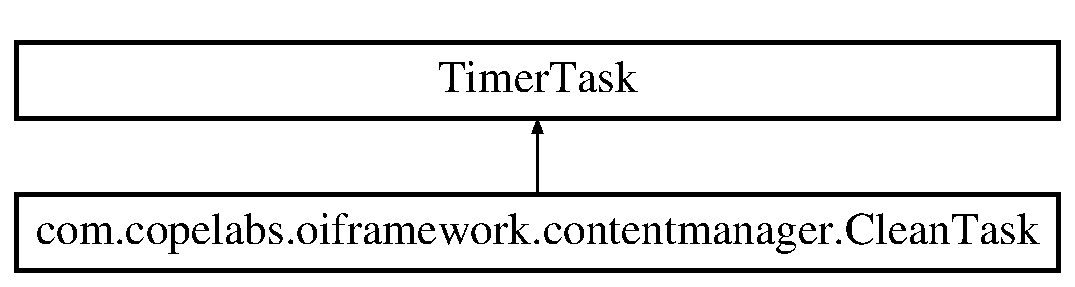
\includegraphics[height=2.000000cm]{classcom_1_1copelabs_1_1oiframework_1_1contentmanager_1_1_clean_task}
\end{center}
\end{figure}
\subsection*{Public Member Functions}
\begin{DoxyCompactItemize}
\item 
\hyperlink{classcom_1_1copelabs_1_1oiframework_1_1contentmanager_1_1_clean_task_a99d62770336a1a3c7ce817c9fbda36cb}{Clean\+Task} ()
\item 
void \hyperlink{classcom_1_1copelabs_1_1oiframework_1_1contentmanager_1_1_clean_task_a357dd2b4ddc2922255cd5ec197a85e39}{run} ()
\end{DoxyCompactItemize}
\subsection*{Private Member Functions}
\begin{DoxyCompactItemize}
\item 
List$<$ \hyperlink{classcom_1_1copelabs_1_1oiframework_1_1contentmanager_1_1_packet}{Packet} $>$ \hyperlink{classcom_1_1copelabs_1_1oiframework_1_1contentmanager_1_1_clean_task_abfb7bdd58804ccde2a98d344a061ca99}{check\+T\+T\+L} (List$<$ \hyperlink{classcom_1_1copelabs_1_1oiframework_1_1contentmanager_1_1_packet}{Packet} $>$ m\+List)
\end{DoxyCompactItemize}
\subsection*{Private Attributes}
\begin{DoxyCompactItemize}
\item 
String \hyperlink{classcom_1_1copelabs_1_1oiframework_1_1contentmanager_1_1_clean_task_af8e9cfc963a1dba3254e7906f9013593}{T\+A\+G} = \char`\"{}T\+T\+L\+\_\+\+Check\char`\"{}
\item 
int \hyperlink{classcom_1_1copelabs_1_1oiframework_1_1contentmanager_1_1_clean_task_a3335ef76525dc81214c4e4f154f67c65}{timeout} = 60000 $\ast$ 60
\end{DoxyCompactItemize}


\subsection{Constructor \& Destructor Documentation}
\hypertarget{classcom_1_1copelabs_1_1oiframework_1_1contentmanager_1_1_clean_task_a99d62770336a1a3c7ce817c9fbda36cb}{}\index{com\+::copelabs\+::oiframework\+::contentmanager\+::\+Clean\+Task@{com\+::copelabs\+::oiframework\+::contentmanager\+::\+Clean\+Task}!Clean\+Task@{Clean\+Task}}
\index{Clean\+Task@{Clean\+Task}!com\+::copelabs\+::oiframework\+::contentmanager\+::\+Clean\+Task@{com\+::copelabs\+::oiframework\+::contentmanager\+::\+Clean\+Task}}
\subsubsection[{Clean\+Task()}]{\setlength{\rightskip}{0pt plus 5cm}com.\+copelabs.\+oiframework.\+contentmanager.\+Clean\+Task.\+Clean\+Task (
\begin{DoxyParamCaption}
{}
\end{DoxyParamCaption}
)}\label{classcom_1_1copelabs_1_1oiframework_1_1contentmanager_1_1_clean_task_a99d62770336a1a3c7ce817c9fbda36cb}


\subsection{Member Function Documentation}
\hypertarget{classcom_1_1copelabs_1_1oiframework_1_1contentmanager_1_1_clean_task_abfb7bdd58804ccde2a98d344a061ca99}{}\index{com\+::copelabs\+::oiframework\+::contentmanager\+::\+Clean\+Task@{com\+::copelabs\+::oiframework\+::contentmanager\+::\+Clean\+Task}!check\+T\+T\+L@{check\+T\+T\+L}}
\index{check\+T\+T\+L@{check\+T\+T\+L}!com\+::copelabs\+::oiframework\+::contentmanager\+::\+Clean\+Task@{com\+::copelabs\+::oiframework\+::contentmanager\+::\+Clean\+Task}}
\subsubsection[{check\+T\+T\+L(\+List$<$ Packet $>$ m\+List)}]{\setlength{\rightskip}{0pt plus 5cm}List$<${\bf Packet}$>$ com.\+copelabs.\+oiframework.\+contentmanager.\+Clean\+Task.\+check\+T\+T\+L (
\begin{DoxyParamCaption}
\item[{List$<$ {\bf Packet} $>$}]{m\+List}
\end{DoxyParamCaption}
)\hspace{0.3cm}{\ttfamily [private]}}\label{classcom_1_1copelabs_1_1oiframework_1_1contentmanager_1_1_clean_task_abfb7bdd58804ccde2a98d344a061ca99}
\hypertarget{classcom_1_1copelabs_1_1oiframework_1_1contentmanager_1_1_clean_task_a357dd2b4ddc2922255cd5ec197a85e39}{}\index{com\+::copelabs\+::oiframework\+::contentmanager\+::\+Clean\+Task@{com\+::copelabs\+::oiframework\+::contentmanager\+::\+Clean\+Task}!run@{run}}
\index{run@{run}!com\+::copelabs\+::oiframework\+::contentmanager\+::\+Clean\+Task@{com\+::copelabs\+::oiframework\+::contentmanager\+::\+Clean\+Task}}
\subsubsection[{run()}]{\setlength{\rightskip}{0pt plus 5cm}void com.\+copelabs.\+oiframework.\+contentmanager.\+Clean\+Task.\+run (
\begin{DoxyParamCaption}
{}
\end{DoxyParamCaption}
)}\label{classcom_1_1copelabs_1_1oiframework_1_1contentmanager_1_1_clean_task_a357dd2b4ddc2922255cd5ec197a85e39}


\subsection{Member Data Documentation}
\hypertarget{classcom_1_1copelabs_1_1oiframework_1_1contentmanager_1_1_clean_task_af8e9cfc963a1dba3254e7906f9013593}{}\index{com\+::copelabs\+::oiframework\+::contentmanager\+::\+Clean\+Task@{com\+::copelabs\+::oiframework\+::contentmanager\+::\+Clean\+Task}!T\+A\+G@{T\+A\+G}}
\index{T\+A\+G@{T\+A\+G}!com\+::copelabs\+::oiframework\+::contentmanager\+::\+Clean\+Task@{com\+::copelabs\+::oiframework\+::contentmanager\+::\+Clean\+Task}}
\subsubsection[{T\+A\+G}]{\setlength{\rightskip}{0pt plus 5cm}String com.\+copelabs.\+oiframework.\+contentmanager.\+Clean\+Task.\+T\+A\+G = \char`\"{}T\+T\+L\+\_\+\+Check\char`\"{}\hspace{0.3cm}{\ttfamily [private]}}\label{classcom_1_1copelabs_1_1oiframework_1_1contentmanager_1_1_clean_task_af8e9cfc963a1dba3254e7906f9013593}
\hypertarget{classcom_1_1copelabs_1_1oiframework_1_1contentmanager_1_1_clean_task_a3335ef76525dc81214c4e4f154f67c65}{}\index{com\+::copelabs\+::oiframework\+::contentmanager\+::\+Clean\+Task@{com\+::copelabs\+::oiframework\+::contentmanager\+::\+Clean\+Task}!timeout@{timeout}}
\index{timeout@{timeout}!com\+::copelabs\+::oiframework\+::contentmanager\+::\+Clean\+Task@{com\+::copelabs\+::oiframework\+::contentmanager\+::\+Clean\+Task}}
\subsubsection[{timeout}]{\setlength{\rightskip}{0pt plus 5cm}int com.\+copelabs.\+oiframework.\+contentmanager.\+Clean\+Task.\+timeout = 60000 $\ast$ 60\hspace{0.3cm}{\ttfamily [private]}}\label{classcom_1_1copelabs_1_1oiframework_1_1contentmanager_1_1_clean_task_a3335ef76525dc81214c4e4f154f67c65}


The documentation for this class was generated from the following file\+:\begin{DoxyCompactItemize}
\item 
src/com/copelabs/oiframework/contentmanager/\hyperlink{_clean_task_8java}{Clean\+Task.\+java}\end{DoxyCompactItemize}

\hypertarget{classcom_1_1copelabs_1_1oiframework_1_1wifi_1_1_client_socket_handler}{}\section{com.\+copelabs.\+oiframework.\+wifi.\+Client\+Socket\+Handler Class Reference}
\label{classcom_1_1copelabs_1_1oiframework_1_1wifi_1_1_client_socket_handler}\index{com.\+copelabs.\+oiframework.\+wifi.\+Client\+Socket\+Handler@{com.\+copelabs.\+oiframework.\+wifi.\+Client\+Socket\+Handler}}
Inheritance diagram for com.\+copelabs.\+oiframework.\+wifi.\+Client\+Socket\+Handler\+:\begin{figure}[H]
\begin{center}
\leavevmode
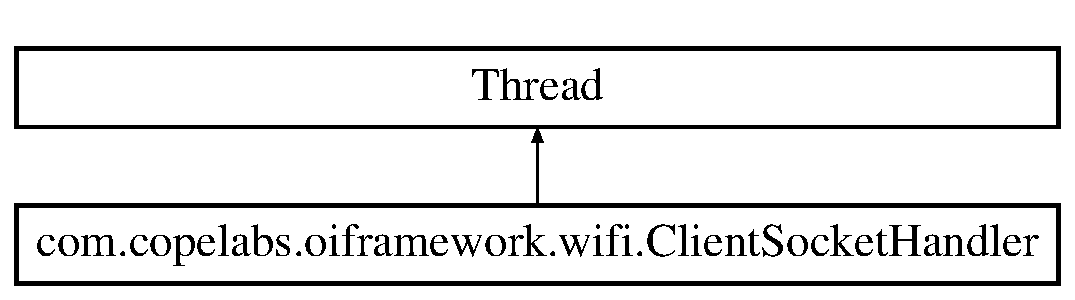
\includegraphics[height=2.000000cm]{classcom_1_1copelabs_1_1oiframework_1_1wifi_1_1_client_socket_handler}
\end{center}
\end{figure}
\subsection*{Public Member Functions}
\begin{DoxyCompactItemize}
\item 
\hyperlink{classcom_1_1copelabs_1_1oiframework_1_1wifi_1_1_client_socket_handler_a943cf10c4b3b72a7de052a573b98fd1b}{Client\+Socket\+Handler} (Handler \hyperlink{classcom_1_1copelabs_1_1oiframework_1_1wifi_1_1_client_socket_handler_a4184a468a1bc27dc42bf1a671e78d87e}{handler}, Inet\+Address group\+Owner\+Address, List$<$ \hyperlink{classcom_1_1copelabs_1_1oiframework_1_1contentmanager_1_1_packet}{Packet} $>$ list, String \hyperlink{classcom_1_1copelabs_1_1oiframework_1_1wifi_1_1_client_socket_handler_a65203e6b9fafa174ef63042dbbec81b4}{m\+This\+Device\+M\+A\+C\+P2p})
\item 
void \hyperlink{classcom_1_1copelabs_1_1oiframework_1_1wifi_1_1_client_socket_handler_accf19ae0519c0d55611d6a28e9620884}{run} ()
\end{DoxyCompactItemize}
\subsection*{Private Attributes}
\begin{DoxyCompactItemize}
\item 
Handler \hyperlink{classcom_1_1copelabs_1_1oiframework_1_1wifi_1_1_client_socket_handler_a4184a468a1bc27dc42bf1a671e78d87e}{handler}
\item 
Inet\+Address \hyperlink{classcom_1_1copelabs_1_1oiframework_1_1wifi_1_1_client_socket_handler_a3284788d2f03622ff3985b1a2f04e0a0}{m\+Address}
\item 
List$<$ \hyperlink{classcom_1_1copelabs_1_1oiframework_1_1contentmanager_1_1_packet}{Packet} $>$ \hyperlink{classcom_1_1copelabs_1_1oiframework_1_1wifi_1_1_client_socket_handler_a7e2770e69e37596bc9d2ca983fe39311}{m\+Data\+To\+Send}
\item 
String \hyperlink{classcom_1_1copelabs_1_1oiframework_1_1wifi_1_1_client_socket_handler_a65203e6b9fafa174ef63042dbbec81b4}{m\+This\+Device\+M\+A\+C\+P2p}
\end{DoxyCompactItemize}
\subsection*{Static Private Attributes}
\begin{DoxyCompactItemize}
\item 
static final String \hyperlink{classcom_1_1copelabs_1_1oiframework_1_1wifi_1_1_client_socket_handler_abca4184271635acce97826e479458213}{T\+A\+G} = \char`\"{}Client\+Socket\+Handler\char`\"{}
\end{DoxyCompactItemize}


\subsection{Constructor \& Destructor Documentation}
\hypertarget{classcom_1_1copelabs_1_1oiframework_1_1wifi_1_1_client_socket_handler_a943cf10c4b3b72a7de052a573b98fd1b}{}\index{com\+::copelabs\+::oiframework\+::wifi\+::\+Client\+Socket\+Handler@{com\+::copelabs\+::oiframework\+::wifi\+::\+Client\+Socket\+Handler}!Client\+Socket\+Handler@{Client\+Socket\+Handler}}
\index{Client\+Socket\+Handler@{Client\+Socket\+Handler}!com\+::copelabs\+::oiframework\+::wifi\+::\+Client\+Socket\+Handler@{com\+::copelabs\+::oiframework\+::wifi\+::\+Client\+Socket\+Handler}}
\subsubsection[{Client\+Socket\+Handler(\+Handler handler, Inet\+Address group\+Owner\+Address, List$<$ Packet $>$ list, String m\+This\+Device\+M\+A\+C\+P2p)}]{\setlength{\rightskip}{0pt plus 5cm}com.\+copelabs.\+oiframework.\+wifi.\+Client\+Socket\+Handler.\+Client\+Socket\+Handler (
\begin{DoxyParamCaption}
\item[{Handler}]{handler, }
\item[{Inet\+Address}]{group\+Owner\+Address, }
\item[{List$<$ {\bf Packet} $>$}]{list, }
\item[{String}]{m\+This\+Device\+M\+A\+C\+P2p}
\end{DoxyParamCaption}
)}\label{classcom_1_1copelabs_1_1oiframework_1_1wifi_1_1_client_socket_handler_a943cf10c4b3b72a7de052a573b98fd1b}


\subsection{Member Function Documentation}
\hypertarget{classcom_1_1copelabs_1_1oiframework_1_1wifi_1_1_client_socket_handler_accf19ae0519c0d55611d6a28e9620884}{}\index{com\+::copelabs\+::oiframework\+::wifi\+::\+Client\+Socket\+Handler@{com\+::copelabs\+::oiframework\+::wifi\+::\+Client\+Socket\+Handler}!run@{run}}
\index{run@{run}!com\+::copelabs\+::oiframework\+::wifi\+::\+Client\+Socket\+Handler@{com\+::copelabs\+::oiframework\+::wifi\+::\+Client\+Socket\+Handler}}
\subsubsection[{run()}]{\setlength{\rightskip}{0pt plus 5cm}void com.\+copelabs.\+oiframework.\+wifi.\+Client\+Socket\+Handler.\+run (
\begin{DoxyParamCaption}
{}
\end{DoxyParamCaption}
)}\label{classcom_1_1copelabs_1_1oiframework_1_1wifi_1_1_client_socket_handler_accf19ae0519c0d55611d6a28e9620884}


\subsection{Member Data Documentation}
\hypertarget{classcom_1_1copelabs_1_1oiframework_1_1wifi_1_1_client_socket_handler_a4184a468a1bc27dc42bf1a671e78d87e}{}\index{com\+::copelabs\+::oiframework\+::wifi\+::\+Client\+Socket\+Handler@{com\+::copelabs\+::oiframework\+::wifi\+::\+Client\+Socket\+Handler}!handler@{handler}}
\index{handler@{handler}!com\+::copelabs\+::oiframework\+::wifi\+::\+Client\+Socket\+Handler@{com\+::copelabs\+::oiframework\+::wifi\+::\+Client\+Socket\+Handler}}
\subsubsection[{handler}]{\setlength{\rightskip}{0pt plus 5cm}Handler com.\+copelabs.\+oiframework.\+wifi.\+Client\+Socket\+Handler.\+handler\hspace{0.3cm}{\ttfamily [private]}}\label{classcom_1_1copelabs_1_1oiframework_1_1wifi_1_1_client_socket_handler_a4184a468a1bc27dc42bf1a671e78d87e}
\hypertarget{classcom_1_1copelabs_1_1oiframework_1_1wifi_1_1_client_socket_handler_a3284788d2f03622ff3985b1a2f04e0a0}{}\index{com\+::copelabs\+::oiframework\+::wifi\+::\+Client\+Socket\+Handler@{com\+::copelabs\+::oiframework\+::wifi\+::\+Client\+Socket\+Handler}!m\+Address@{m\+Address}}
\index{m\+Address@{m\+Address}!com\+::copelabs\+::oiframework\+::wifi\+::\+Client\+Socket\+Handler@{com\+::copelabs\+::oiframework\+::wifi\+::\+Client\+Socket\+Handler}}
\subsubsection[{m\+Address}]{\setlength{\rightskip}{0pt plus 5cm}Inet\+Address com.\+copelabs.\+oiframework.\+wifi.\+Client\+Socket\+Handler.\+m\+Address\hspace{0.3cm}{\ttfamily [private]}}\label{classcom_1_1copelabs_1_1oiframework_1_1wifi_1_1_client_socket_handler_a3284788d2f03622ff3985b1a2f04e0a0}
\hypertarget{classcom_1_1copelabs_1_1oiframework_1_1wifi_1_1_client_socket_handler_a7e2770e69e37596bc9d2ca983fe39311}{}\index{com\+::copelabs\+::oiframework\+::wifi\+::\+Client\+Socket\+Handler@{com\+::copelabs\+::oiframework\+::wifi\+::\+Client\+Socket\+Handler}!m\+Data\+To\+Send@{m\+Data\+To\+Send}}
\index{m\+Data\+To\+Send@{m\+Data\+To\+Send}!com\+::copelabs\+::oiframework\+::wifi\+::\+Client\+Socket\+Handler@{com\+::copelabs\+::oiframework\+::wifi\+::\+Client\+Socket\+Handler}}
\subsubsection[{m\+Data\+To\+Send}]{\setlength{\rightskip}{0pt plus 5cm}List$<${\bf Packet}$>$ com.\+copelabs.\+oiframework.\+wifi.\+Client\+Socket\+Handler.\+m\+Data\+To\+Send\hspace{0.3cm}{\ttfamily [private]}}\label{classcom_1_1copelabs_1_1oiframework_1_1wifi_1_1_client_socket_handler_a7e2770e69e37596bc9d2ca983fe39311}
\hypertarget{classcom_1_1copelabs_1_1oiframework_1_1wifi_1_1_client_socket_handler_a65203e6b9fafa174ef63042dbbec81b4}{}\index{com\+::copelabs\+::oiframework\+::wifi\+::\+Client\+Socket\+Handler@{com\+::copelabs\+::oiframework\+::wifi\+::\+Client\+Socket\+Handler}!m\+This\+Device\+M\+A\+C\+P2p@{m\+This\+Device\+M\+A\+C\+P2p}}
\index{m\+This\+Device\+M\+A\+C\+P2p@{m\+This\+Device\+M\+A\+C\+P2p}!com\+::copelabs\+::oiframework\+::wifi\+::\+Client\+Socket\+Handler@{com\+::copelabs\+::oiframework\+::wifi\+::\+Client\+Socket\+Handler}}
\subsubsection[{m\+This\+Device\+M\+A\+C\+P2p}]{\setlength{\rightskip}{0pt plus 5cm}String com.\+copelabs.\+oiframework.\+wifi.\+Client\+Socket\+Handler.\+m\+This\+Device\+M\+A\+C\+P2p\hspace{0.3cm}{\ttfamily [private]}}\label{classcom_1_1copelabs_1_1oiframework_1_1wifi_1_1_client_socket_handler_a65203e6b9fafa174ef63042dbbec81b4}
\hypertarget{classcom_1_1copelabs_1_1oiframework_1_1wifi_1_1_client_socket_handler_abca4184271635acce97826e479458213}{}\index{com\+::copelabs\+::oiframework\+::wifi\+::\+Client\+Socket\+Handler@{com\+::copelabs\+::oiframework\+::wifi\+::\+Client\+Socket\+Handler}!T\+A\+G@{T\+A\+G}}
\index{T\+A\+G@{T\+A\+G}!com\+::copelabs\+::oiframework\+::wifi\+::\+Client\+Socket\+Handler@{com\+::copelabs\+::oiframework\+::wifi\+::\+Client\+Socket\+Handler}}
\subsubsection[{T\+A\+G}]{\setlength{\rightskip}{0pt plus 5cm}final String com.\+copelabs.\+oiframework.\+wifi.\+Client\+Socket\+Handler.\+T\+A\+G = \char`\"{}Client\+Socket\+Handler\char`\"{}\hspace{0.3cm}{\ttfamily [static]}, {\ttfamily [private]}}\label{classcom_1_1copelabs_1_1oiframework_1_1wifi_1_1_client_socket_handler_abca4184271635acce97826e479458213}


The documentation for this class was generated from the following file\+:\begin{DoxyCompactItemize}
\item 
src/com/copelabs/oiframework/wifi/\hyperlink{_client_socket_handler_8java}{Client\+Socket\+Handler.\+java}\end{DoxyCompactItemize}

\hypertarget{classcom_1_1copelabs_1_1oiframework_1_1contentmanager_1_1_content_manager}{}\section{com.\+copelabs.\+oiframework.\+contentmanager.\+Content\+Manager Class Reference}
\label{classcom_1_1copelabs_1_1oiframework_1_1contentmanager_1_1_content_manager}\index{com.\+copelabs.\+oiframework.\+contentmanager.\+Content\+Manager@{com.\+copelabs.\+oiframework.\+contentmanager.\+Content\+Manager}}
Inheritance diagram for com.\+copelabs.\+oiframework.\+contentmanager.\+Content\+Manager\+:\begin{figure}[H]
\begin{center}
\leavevmode
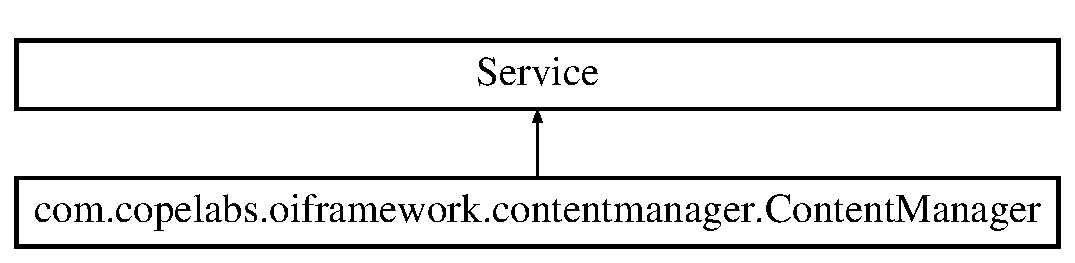
\includegraphics[height=2.000000cm]{classcom_1_1copelabs_1_1oiframework_1_1contentmanager_1_1_content_manager}
\end{center}
\end{figure}
\subsection*{Public Member Functions}
\begin{DoxyCompactItemize}
\item 
void \hyperlink{classcom_1_1copelabs_1_1oiframework_1_1contentmanager_1_1_content_manager_a82247d9b6404ed835f30322e4d9d555c}{on\+Create} ()
\item 
void \hyperlink{classcom_1_1copelabs_1_1oiframework_1_1contentmanager_1_1_content_manager_a044b9fff26d4a9ad967cbacd0ac967bd}{on\+Destroy} ()
\item 
I\+Binder \hyperlink{classcom_1_1copelabs_1_1oiframework_1_1contentmanager_1_1_content_manager_a4f0e6894e934e8f67a51f311af90ee19}{on\+Bind} (Intent intent)
\end{DoxyCompactItemize}
\subsection*{Private Member Functions}
\begin{DoxyCompactItemize}
\item 
void \hyperlink{classcom_1_1copelabs_1_1oiframework_1_1contentmanager_1_1_content_manager_aa48dc62ec9f9588a1eccfc532519a9b1}{initialize\+Modules} ()
\item 
void \hyperlink{classcom_1_1copelabs_1_1oiframework_1_1contentmanager_1_1_content_manager_aff3f09048a8e2950db68b814784135be}{init\+T\+T\+L\+\_\+\+Timer} ()
\item 
boolean \hyperlink{classcom_1_1copelabs_1_1oiframework_1_1contentmanager_1_1_content_manager_a843d5651fb973b0ba921010858592cf9}{send\+Packet\+To\+App} (\hyperlink{classcom_1_1copelabs_1_1oiframework_1_1contentmanager_1_1_packet}{Packet} m\+Packet)
\item 
void \hyperlink{classcom_1_1copelabs_1_1oiframework_1_1contentmanager_1_1_content_manager_a6efcf27814c50d4fdca421d929c8ac7d}{receive\+Packet} (List$<$ \hyperlink{classcom_1_1copelabs_1_1oiframework_1_1contentmanager_1_1_packet}{Packet} $>$ m\+List\+Of\+Packets)
\item 
boolean \hyperlink{classcom_1_1copelabs_1_1oiframework_1_1contentmanager_1_1_content_manager_a398ef49c6126668a488e7f41cb26a732}{is\+Packet\+Duplicated} (\hyperlink{classcom_1_1copelabs_1_1oiframework_1_1contentmanager_1_1_packet}{Packet} m\+New\+Packet, String m\+File)
\item 
void \hyperlink{classcom_1_1copelabs_1_1oiframework_1_1contentmanager_1_1_content_manager_a44e01742b6c02503c2b9949cf68ae372}{new\+Device\+Found\+To\+App} (User\+Device m\+Device)
\item 
void \hyperlink{classcom_1_1copelabs_1_1oiframework_1_1contentmanager_1_1_content_manager_a9223b3fb51dfb77db68652dbdd6d1c97}{device\+Lost\+To\+App} (User\+Device m\+Device)
\item 
void \hyperlink{classcom_1_1copelabs_1_1oiframework_1_1contentmanager_1_1_content_manager_a39ef377cc2c6398ec52253bb5b362aec}{send\+Error} (int m\+Error)
\item 
void \hyperlink{classcom_1_1copelabs_1_1oiframework_1_1contentmanager_1_1_content_manager_aeffc5e72d64f214dbe1b744b2f2565b9}{contact\+List\+Updated\+To\+App} (List$<$ User\+Device $>$ m\+List)
\end{DoxyCompactItemize}
\subsection*{Private Attributes}
\begin{DoxyCompactItemize}
\item 
\hyperlink{classcom_1_1copelabs_1_1oiframework_1_1router_1_1_routing}{Routing} \hyperlink{classcom_1_1copelabs_1_1oiframework_1_1contentmanager_1_1_content_manager_a15b9d671e7079dd1c471a4b6a331f3e8}{p\+Routing}
\item 
int \hyperlink{classcom_1_1copelabs_1_1oiframework_1_1contentmanager_1_1_content_manager_a804a8e78c97fca907d1752b0176a1a57}{interface\+Enabled} = 1
\item 
final I\+Remote\+Oi\+Framework.\+Stub \hyperlink{classcom_1_1copelabs_1_1oiframework_1_1contentmanager_1_1_content_manager_a530fa8b90c4758fdbad5f0973ea488e8}{m\+Binder}
\end{DoxyCompactItemize}
\subsection*{Static Private Attributes}
\begin{DoxyCompactItemize}
\item 
static final String \hyperlink{classcom_1_1copelabs_1_1oiframework_1_1contentmanager_1_1_content_manager_a5768346882b7f03d78b3e2e09ff482fa}{T\+A\+G} = \char`\"{}Oi\+Service\char`\"{}
\item 
static final String \hyperlink{classcom_1_1copelabs_1_1oiframework_1_1contentmanager_1_1_content_manager_a54253c268f02b62bf5db606859ab7b5b}{T\+A\+G2} = \char`\"{}Oi Demo\char`\"{}
\end{DoxyCompactItemize}


\subsection{Member Function Documentation}
\hypertarget{classcom_1_1copelabs_1_1oiframework_1_1contentmanager_1_1_content_manager_aeffc5e72d64f214dbe1b744b2f2565b9}{}\index{com\+::copelabs\+::oiframework\+::contentmanager\+::\+Content\+Manager@{com\+::copelabs\+::oiframework\+::contentmanager\+::\+Content\+Manager}!contact\+List\+Updated\+To\+App@{contact\+List\+Updated\+To\+App}}
\index{contact\+List\+Updated\+To\+App@{contact\+List\+Updated\+To\+App}!com\+::copelabs\+::oiframework\+::contentmanager\+::\+Content\+Manager@{com\+::copelabs\+::oiframework\+::contentmanager\+::\+Content\+Manager}}
\subsubsection[{contact\+List\+Updated\+To\+App(\+List$<$ User\+Device $>$ m\+List)}]{\setlength{\rightskip}{0pt plus 5cm}void com.\+copelabs.\+oiframework.\+contentmanager.\+Content\+Manager.\+contact\+List\+Updated\+To\+App (
\begin{DoxyParamCaption}
\item[{List$<$ User\+Device $>$}]{m\+List}
\end{DoxyParamCaption}
)\hspace{0.3cm}{\ttfamily [private]}}\label{classcom_1_1copelabs_1_1oiframework_1_1contentmanager_1_1_content_manager_aeffc5e72d64f214dbe1b744b2f2565b9}
\hypertarget{classcom_1_1copelabs_1_1oiframework_1_1contentmanager_1_1_content_manager_a9223b3fb51dfb77db68652dbdd6d1c97}{}\index{com\+::copelabs\+::oiframework\+::contentmanager\+::\+Content\+Manager@{com\+::copelabs\+::oiframework\+::contentmanager\+::\+Content\+Manager}!device\+Lost\+To\+App@{device\+Lost\+To\+App}}
\index{device\+Lost\+To\+App@{device\+Lost\+To\+App}!com\+::copelabs\+::oiframework\+::contentmanager\+::\+Content\+Manager@{com\+::copelabs\+::oiframework\+::contentmanager\+::\+Content\+Manager}}
\subsubsection[{device\+Lost\+To\+App(\+User\+Device m\+Device)}]{\setlength{\rightskip}{0pt plus 5cm}void com.\+copelabs.\+oiframework.\+contentmanager.\+Content\+Manager.\+device\+Lost\+To\+App (
\begin{DoxyParamCaption}
\item[{User\+Device}]{m\+Device}
\end{DoxyParamCaption}
)\hspace{0.3cm}{\ttfamily [private]}}\label{classcom_1_1copelabs_1_1oiframework_1_1contentmanager_1_1_content_manager_a9223b3fb51dfb77db68652dbdd6d1c97}
\hypertarget{classcom_1_1copelabs_1_1oiframework_1_1contentmanager_1_1_content_manager_aa48dc62ec9f9588a1eccfc532519a9b1}{}\index{com\+::copelabs\+::oiframework\+::contentmanager\+::\+Content\+Manager@{com\+::copelabs\+::oiframework\+::contentmanager\+::\+Content\+Manager}!initialize\+Modules@{initialize\+Modules}}
\index{initialize\+Modules@{initialize\+Modules}!com\+::copelabs\+::oiframework\+::contentmanager\+::\+Content\+Manager@{com\+::copelabs\+::oiframework\+::contentmanager\+::\+Content\+Manager}}
\subsubsection[{initialize\+Modules()}]{\setlength{\rightskip}{0pt plus 5cm}void com.\+copelabs.\+oiframework.\+contentmanager.\+Content\+Manager.\+initialize\+Modules (
\begin{DoxyParamCaption}
{}
\end{DoxyParamCaption}
)\hspace{0.3cm}{\ttfamily [private]}}\label{classcom_1_1copelabs_1_1oiframework_1_1contentmanager_1_1_content_manager_aa48dc62ec9f9588a1eccfc532519a9b1}
\hypertarget{classcom_1_1copelabs_1_1oiframework_1_1contentmanager_1_1_content_manager_aff3f09048a8e2950db68b814784135be}{}\index{com\+::copelabs\+::oiframework\+::contentmanager\+::\+Content\+Manager@{com\+::copelabs\+::oiframework\+::contentmanager\+::\+Content\+Manager}!init\+T\+T\+L\+\_\+\+Timer@{init\+T\+T\+L\+\_\+\+Timer}}
\index{init\+T\+T\+L\+\_\+\+Timer@{init\+T\+T\+L\+\_\+\+Timer}!com\+::copelabs\+::oiframework\+::contentmanager\+::\+Content\+Manager@{com\+::copelabs\+::oiframework\+::contentmanager\+::\+Content\+Manager}}
\subsubsection[{init\+T\+T\+L\+\_\+\+Timer()}]{\setlength{\rightskip}{0pt plus 5cm}void com.\+copelabs.\+oiframework.\+contentmanager.\+Content\+Manager.\+init\+T\+T\+L\+\_\+\+Timer (
\begin{DoxyParamCaption}
{}
\end{DoxyParamCaption}
)\hspace{0.3cm}{\ttfamily [private]}}\label{classcom_1_1copelabs_1_1oiframework_1_1contentmanager_1_1_content_manager_aff3f09048a8e2950db68b814784135be}
\hypertarget{classcom_1_1copelabs_1_1oiframework_1_1contentmanager_1_1_content_manager_a398ef49c6126668a488e7f41cb26a732}{}\index{com\+::copelabs\+::oiframework\+::contentmanager\+::\+Content\+Manager@{com\+::copelabs\+::oiframework\+::contentmanager\+::\+Content\+Manager}!is\+Packet\+Duplicated@{is\+Packet\+Duplicated}}
\index{is\+Packet\+Duplicated@{is\+Packet\+Duplicated}!com\+::copelabs\+::oiframework\+::contentmanager\+::\+Content\+Manager@{com\+::copelabs\+::oiframework\+::contentmanager\+::\+Content\+Manager}}
\subsubsection[{is\+Packet\+Duplicated(\+Packet m\+New\+Packet, String m\+File)}]{\setlength{\rightskip}{0pt plus 5cm}boolean com.\+copelabs.\+oiframework.\+contentmanager.\+Content\+Manager.\+is\+Packet\+Duplicated (
\begin{DoxyParamCaption}
\item[{{\bf Packet}}]{m\+New\+Packet, }
\item[{String}]{m\+File}
\end{DoxyParamCaption}
)\hspace{0.3cm}{\ttfamily [private]}}\label{classcom_1_1copelabs_1_1oiframework_1_1contentmanager_1_1_content_manager_a398ef49c6126668a488e7f41cb26a732}
Check if the new packet received is already saved inside the Local Cache file 
\begin{DoxyParams}{Parameters}
{\em m\+New\+Packet} & \hyperlink{classcom_1_1copelabs_1_1oiframework_1_1contentmanager_1_1_packet}{Packet} to check if it this duplicated \\
\hline
\end{DoxyParams}
\begin{DoxyReturn}{Returns}
true if is already available at local cache or false if not. 
\end{DoxyReturn}
\hypertarget{classcom_1_1copelabs_1_1oiframework_1_1contentmanager_1_1_content_manager_a44e01742b6c02503c2b9949cf68ae372}{}\index{com\+::copelabs\+::oiframework\+::contentmanager\+::\+Content\+Manager@{com\+::copelabs\+::oiframework\+::contentmanager\+::\+Content\+Manager}!new\+Device\+Found\+To\+App@{new\+Device\+Found\+To\+App}}
\index{new\+Device\+Found\+To\+App@{new\+Device\+Found\+To\+App}!com\+::copelabs\+::oiframework\+::contentmanager\+::\+Content\+Manager@{com\+::copelabs\+::oiframework\+::contentmanager\+::\+Content\+Manager}}
\subsubsection[{new\+Device\+Found\+To\+App(\+User\+Device m\+Device)}]{\setlength{\rightskip}{0pt plus 5cm}void com.\+copelabs.\+oiframework.\+contentmanager.\+Content\+Manager.\+new\+Device\+Found\+To\+App (
\begin{DoxyParamCaption}
\item[{User\+Device}]{m\+Device}
\end{DoxyParamCaption}
)\hspace{0.3cm}{\ttfamily [private]}}\label{classcom_1_1copelabs_1_1oiframework_1_1contentmanager_1_1_content_manager_a44e01742b6c02503c2b9949cf68ae372}
\hypertarget{classcom_1_1copelabs_1_1oiframework_1_1contentmanager_1_1_content_manager_a4f0e6894e934e8f67a51f311af90ee19}{}\index{com\+::copelabs\+::oiframework\+::contentmanager\+::\+Content\+Manager@{com\+::copelabs\+::oiframework\+::contentmanager\+::\+Content\+Manager}!on\+Bind@{on\+Bind}}
\index{on\+Bind@{on\+Bind}!com\+::copelabs\+::oiframework\+::contentmanager\+::\+Content\+Manager@{com\+::copelabs\+::oiframework\+::contentmanager\+::\+Content\+Manager}}
\subsubsection[{on\+Bind(\+Intent intent)}]{\setlength{\rightskip}{0pt plus 5cm}I\+Binder com.\+copelabs.\+oiframework.\+contentmanager.\+Content\+Manager.\+on\+Bind (
\begin{DoxyParamCaption}
\item[{Intent}]{intent}
\end{DoxyParamCaption}
)}\label{classcom_1_1copelabs_1_1oiframework_1_1contentmanager_1_1_content_manager_a4f0e6894e934e8f67a51f311af90ee19}
\hypertarget{classcom_1_1copelabs_1_1oiframework_1_1contentmanager_1_1_content_manager_a82247d9b6404ed835f30322e4d9d555c}{}\index{com\+::copelabs\+::oiframework\+::contentmanager\+::\+Content\+Manager@{com\+::copelabs\+::oiframework\+::contentmanager\+::\+Content\+Manager}!on\+Create@{on\+Create}}
\index{on\+Create@{on\+Create}!com\+::copelabs\+::oiframework\+::contentmanager\+::\+Content\+Manager@{com\+::copelabs\+::oiframework\+::contentmanager\+::\+Content\+Manager}}
\subsubsection[{on\+Create()}]{\setlength{\rightskip}{0pt plus 5cm}void com.\+copelabs.\+oiframework.\+contentmanager.\+Content\+Manager.\+on\+Create (
\begin{DoxyParamCaption}
{}
\end{DoxyParamCaption}
)}\label{classcom_1_1copelabs_1_1oiframework_1_1contentmanager_1_1_content_manager_a82247d9b6404ed835f30322e4d9d555c}
\hypertarget{classcom_1_1copelabs_1_1oiframework_1_1contentmanager_1_1_content_manager_a044b9fff26d4a9ad967cbacd0ac967bd}{}\index{com\+::copelabs\+::oiframework\+::contentmanager\+::\+Content\+Manager@{com\+::copelabs\+::oiframework\+::contentmanager\+::\+Content\+Manager}!on\+Destroy@{on\+Destroy}}
\index{on\+Destroy@{on\+Destroy}!com\+::copelabs\+::oiframework\+::contentmanager\+::\+Content\+Manager@{com\+::copelabs\+::oiframework\+::contentmanager\+::\+Content\+Manager}}
\subsubsection[{on\+Destroy()}]{\setlength{\rightskip}{0pt plus 5cm}void com.\+copelabs.\+oiframework.\+contentmanager.\+Content\+Manager.\+on\+Destroy (
\begin{DoxyParamCaption}
{}
\end{DoxyParamCaption}
)}\label{classcom_1_1copelabs_1_1oiframework_1_1contentmanager_1_1_content_manager_a044b9fff26d4a9ad967cbacd0ac967bd}
\hypertarget{classcom_1_1copelabs_1_1oiframework_1_1contentmanager_1_1_content_manager_a6efcf27814c50d4fdca421d929c8ac7d}{}\index{com\+::copelabs\+::oiframework\+::contentmanager\+::\+Content\+Manager@{com\+::copelabs\+::oiframework\+::contentmanager\+::\+Content\+Manager}!receive\+Packet@{receive\+Packet}}
\index{receive\+Packet@{receive\+Packet}!com\+::copelabs\+::oiframework\+::contentmanager\+::\+Content\+Manager@{com\+::copelabs\+::oiframework\+::contentmanager\+::\+Content\+Manager}}
\subsubsection[{receive\+Packet(\+List$<$ Packet $>$ m\+List\+Of\+Packets)}]{\setlength{\rightskip}{0pt plus 5cm}void com.\+copelabs.\+oiframework.\+contentmanager.\+Content\+Manager.\+receive\+Packet (
\begin{DoxyParamCaption}
\item[{List$<$ {\bf Packet} $>$}]{m\+List\+Of\+Packets}
\end{DoxyParamCaption}
)\hspace{0.3cm}{\ttfamily [private]}}\label{classcom_1_1copelabs_1_1oiframework_1_1contentmanager_1_1_content_manager_a6efcf27814c50d4fdca421d929c8ac7d}
Method used by the others packages, when a new packet arrived. It checks if the packet is for this device. If it is, tries to send to the correct app. If not saves the packet to a file. 
\begin{DoxyParams}{Parameters}
{\em m\+Packet} & \\
\hline
\end{DoxyParams}
\hypertarget{classcom_1_1copelabs_1_1oiframework_1_1contentmanager_1_1_content_manager_a39ef377cc2c6398ec52253bb5b362aec}{}\index{com\+::copelabs\+::oiframework\+::contentmanager\+::\+Content\+Manager@{com\+::copelabs\+::oiframework\+::contentmanager\+::\+Content\+Manager}!send\+Error@{send\+Error}}
\index{send\+Error@{send\+Error}!com\+::copelabs\+::oiframework\+::contentmanager\+::\+Content\+Manager@{com\+::copelabs\+::oiframework\+::contentmanager\+::\+Content\+Manager}}
\subsubsection[{send\+Error(int m\+Error)}]{\setlength{\rightskip}{0pt plus 5cm}void com.\+copelabs.\+oiframework.\+contentmanager.\+Content\+Manager.\+send\+Error (
\begin{DoxyParamCaption}
\item[{int}]{m\+Error}
\end{DoxyParamCaption}
)\hspace{0.3cm}{\ttfamily [private]}}\label{classcom_1_1copelabs_1_1oiframework_1_1contentmanager_1_1_content_manager_a39ef377cc2c6398ec52253bb5b362aec}
\hypertarget{classcom_1_1copelabs_1_1oiframework_1_1contentmanager_1_1_content_manager_a843d5651fb973b0ba921010858592cf9}{}\index{com\+::copelabs\+::oiframework\+::contentmanager\+::\+Content\+Manager@{com\+::copelabs\+::oiframework\+::contentmanager\+::\+Content\+Manager}!send\+Packet\+To\+App@{send\+Packet\+To\+App}}
\index{send\+Packet\+To\+App@{send\+Packet\+To\+App}!com\+::copelabs\+::oiframework\+::contentmanager\+::\+Content\+Manager@{com\+::copelabs\+::oiframework\+::contentmanager\+::\+Content\+Manager}}
\subsubsection[{send\+Packet\+To\+App(\+Packet m\+Packet)}]{\setlength{\rightskip}{0pt plus 5cm}boolean com.\+copelabs.\+oiframework.\+contentmanager.\+Content\+Manager.\+send\+Packet\+To\+App (
\begin{DoxyParamCaption}
\item[{{\bf Packet}}]{m\+Packet}
\end{DoxyParamCaption}
)\hspace{0.3cm}{\ttfamily [private]}}\label{classcom_1_1copelabs_1_1oiframework_1_1contentmanager_1_1_content_manager_a843d5651fb973b0ba921010858592cf9}
Method the tries to send the packet to the correct app. 
\begin{DoxyParams}{Parameters}
{\em m\+Packet} & \\
\hline
\end{DoxyParams}
\begin{DoxyReturn}{Returns}
true if packet was successfully sent, false if app is not available (callback not registered) 
\end{DoxyReturn}


\subsection{Member Data Documentation}
\hypertarget{classcom_1_1copelabs_1_1oiframework_1_1contentmanager_1_1_content_manager_a804a8e78c97fca907d1752b0176a1a57}{}\index{com\+::copelabs\+::oiframework\+::contentmanager\+::\+Content\+Manager@{com\+::copelabs\+::oiframework\+::contentmanager\+::\+Content\+Manager}!interface\+Enabled@{interface\+Enabled}}
\index{interface\+Enabled@{interface\+Enabled}!com\+::copelabs\+::oiframework\+::contentmanager\+::\+Content\+Manager@{com\+::copelabs\+::oiframework\+::contentmanager\+::\+Content\+Manager}}
\subsubsection[{interface\+Enabled}]{\setlength{\rightskip}{0pt plus 5cm}int com.\+copelabs.\+oiframework.\+contentmanager.\+Content\+Manager.\+interface\+Enabled = 1\hspace{0.3cm}{\ttfamily [private]}}\label{classcom_1_1copelabs_1_1oiframework_1_1contentmanager_1_1_content_manager_a804a8e78c97fca907d1752b0176a1a57}
\hypertarget{classcom_1_1copelabs_1_1oiframework_1_1contentmanager_1_1_content_manager_a530fa8b90c4758fdbad5f0973ea488e8}{}\index{com\+::copelabs\+::oiframework\+::contentmanager\+::\+Content\+Manager@{com\+::copelabs\+::oiframework\+::contentmanager\+::\+Content\+Manager}!m\+Binder@{m\+Binder}}
\index{m\+Binder@{m\+Binder}!com\+::copelabs\+::oiframework\+::contentmanager\+::\+Content\+Manager@{com\+::copelabs\+::oiframework\+::contentmanager\+::\+Content\+Manager}}
\subsubsection[{m\+Binder}]{\setlength{\rightskip}{0pt plus 5cm}final I\+Remote\+Oi\+Framework.\+Stub com.\+copelabs.\+oiframework.\+contentmanager.\+Content\+Manager.\+m\+Binder\hspace{0.3cm}{\ttfamily [private]}}\label{classcom_1_1copelabs_1_1oiframework_1_1contentmanager_1_1_content_manager_a530fa8b90c4758fdbad5f0973ea488e8}
\hypertarget{classcom_1_1copelabs_1_1oiframework_1_1contentmanager_1_1_content_manager_a15b9d671e7079dd1c471a4b6a331f3e8}{}\index{com\+::copelabs\+::oiframework\+::contentmanager\+::\+Content\+Manager@{com\+::copelabs\+::oiframework\+::contentmanager\+::\+Content\+Manager}!p\+Routing@{p\+Routing}}
\index{p\+Routing@{p\+Routing}!com\+::copelabs\+::oiframework\+::contentmanager\+::\+Content\+Manager@{com\+::copelabs\+::oiframework\+::contentmanager\+::\+Content\+Manager}}
\subsubsection[{p\+Routing}]{\setlength{\rightskip}{0pt plus 5cm}{\bf Routing} com.\+copelabs.\+oiframework.\+contentmanager.\+Content\+Manager.\+p\+Routing\hspace{0.3cm}{\ttfamily [private]}}\label{classcom_1_1copelabs_1_1oiframework_1_1contentmanager_1_1_content_manager_a15b9d671e7079dd1c471a4b6a331f3e8}
\hypertarget{classcom_1_1copelabs_1_1oiframework_1_1contentmanager_1_1_content_manager_a5768346882b7f03d78b3e2e09ff482fa}{}\index{com\+::copelabs\+::oiframework\+::contentmanager\+::\+Content\+Manager@{com\+::copelabs\+::oiframework\+::contentmanager\+::\+Content\+Manager}!T\+A\+G@{T\+A\+G}}
\index{T\+A\+G@{T\+A\+G}!com\+::copelabs\+::oiframework\+::contentmanager\+::\+Content\+Manager@{com\+::copelabs\+::oiframework\+::contentmanager\+::\+Content\+Manager}}
\subsubsection[{T\+A\+G}]{\setlength{\rightskip}{0pt plus 5cm}final String com.\+copelabs.\+oiframework.\+contentmanager.\+Content\+Manager.\+T\+A\+G = \char`\"{}Oi\+Service\char`\"{}\hspace{0.3cm}{\ttfamily [static]}, {\ttfamily [private]}}\label{classcom_1_1copelabs_1_1oiframework_1_1contentmanager_1_1_content_manager_a5768346882b7f03d78b3e2e09ff482fa}
Follow Field Naming Conventions

Non-\/public, non-\/static field names start with m. Static field names start with s. Other fields start with a lower case letter. m stands for member variable or data member. Public static final fields (constants) are A\+L\+L\+\_\+\+C\+A\+P\+S\+\_\+\+W\+I\+T\+H\+\_\+\+U\+N\+D\+E\+R\+S\+C\+O\+R\+E\+S. \hypertarget{classcom_1_1copelabs_1_1oiframework_1_1contentmanager_1_1_content_manager_a54253c268f02b62bf5db606859ab7b5b}{}\index{com\+::copelabs\+::oiframework\+::contentmanager\+::\+Content\+Manager@{com\+::copelabs\+::oiframework\+::contentmanager\+::\+Content\+Manager}!T\+A\+G2@{T\+A\+G2}}
\index{T\+A\+G2@{T\+A\+G2}!com\+::copelabs\+::oiframework\+::contentmanager\+::\+Content\+Manager@{com\+::copelabs\+::oiframework\+::contentmanager\+::\+Content\+Manager}}
\subsubsection[{T\+A\+G2}]{\setlength{\rightskip}{0pt plus 5cm}final String com.\+copelabs.\+oiframework.\+contentmanager.\+Content\+Manager.\+T\+A\+G2 = \char`\"{}Oi Demo\char`\"{}\hspace{0.3cm}{\ttfamily [static]}, {\ttfamily [private]}}\label{classcom_1_1copelabs_1_1oiframework_1_1contentmanager_1_1_content_manager_a54253c268f02b62bf5db606859ab7b5b}


The documentation for this class was generated from the following file\+:\begin{DoxyCompactItemize}
\item 
src/com/copelabs/oiframework/contentmanager/\hyperlink{_content_manager_8java}{Content\+Manager.\+java}\end{DoxyCompactItemize}

\hypertarget{classcom_1_1copelabs_1_1oiframework_1_1socialproximity_1_1_social_proximity_1_1_custom_comparator}{}\section{com.\+copelabs.\+oiframework.\+socialproximity.\+Social\+Proximity.\+Custom\+Comparator Class Reference}
\label{classcom_1_1copelabs_1_1oiframework_1_1socialproximity_1_1_social_proximity_1_1_custom_comparator}\index{com.\+copelabs.\+oiframework.\+socialproximity.\+Social\+Proximity.\+Custom\+Comparator@{com.\+copelabs.\+oiframework.\+socialproximity.\+Social\+Proximity.\+Custom\+Comparator}}
Inheritance diagram for com.\+copelabs.\+oiframework.\+socialproximity.\+Social\+Proximity.\+Custom\+Comparator\+:\begin{figure}[H]
\begin{center}
\leavevmode
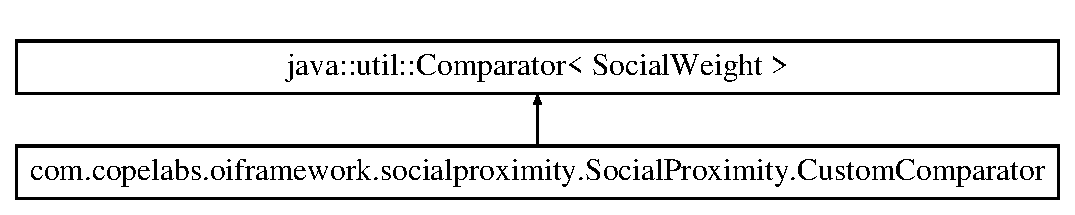
\includegraphics[height=2.000000cm]{classcom_1_1copelabs_1_1oiframework_1_1socialproximity_1_1_social_proximity_1_1_custom_comparator}
\end{center}
\end{figure}
\subsection*{Public Member Functions}
\begin{DoxyCompactItemize}
\item 
int \hyperlink{classcom_1_1copelabs_1_1oiframework_1_1socialproximity_1_1_social_proximity_1_1_custom_comparator_a30b2445a2b4d3437420259a6882d30e9}{compare} (\hyperlink{classcom_1_1copelabs_1_1oiframework_1_1socialproximity_1_1_social_weight}{Social\+Weight} entry1, \hyperlink{classcom_1_1copelabs_1_1oiframework_1_1socialproximity_1_1_social_weight}{Social\+Weight} entry2)
\end{DoxyCompactItemize}


\subsection{Detailed Description}
This class allows to sort social weight entries in ascending order. 

\subsection{Member Function Documentation}
\hypertarget{classcom_1_1copelabs_1_1oiframework_1_1socialproximity_1_1_social_proximity_1_1_custom_comparator_a30b2445a2b4d3437420259a6882d30e9}{}\index{com\+::copelabs\+::oiframework\+::socialproximity\+::\+Social\+Proximity\+::\+Custom\+Comparator@{com\+::copelabs\+::oiframework\+::socialproximity\+::\+Social\+Proximity\+::\+Custom\+Comparator}!compare@{compare}}
\index{compare@{compare}!com\+::copelabs\+::oiframework\+::socialproximity\+::\+Social\+Proximity\+::\+Custom\+Comparator@{com\+::copelabs\+::oiframework\+::socialproximity\+::\+Social\+Proximity\+::\+Custom\+Comparator}}
\subsubsection[{compare(\+Social\+Weight entry1, Social\+Weight entry2)}]{\setlength{\rightskip}{0pt plus 5cm}int com.\+copelabs.\+oiframework.\+socialproximity.\+Social\+Proximity.\+Custom\+Comparator.\+compare (
\begin{DoxyParamCaption}
\item[{{\bf Social\+Weight}}]{entry1, }
\item[{{\bf Social\+Weight}}]{entry2}
\end{DoxyParamCaption}
)}\label{classcom_1_1copelabs_1_1oiframework_1_1socialproximity_1_1_social_proximity_1_1_custom_comparator_a30b2445a2b4d3437420259a6882d30e9}


The documentation for this class was generated from the following file\+:\begin{DoxyCompactItemize}
\item 
src/com/copelabs/oiframework/socialproximity/\hyperlink{_social_proximity_8java}{Social\+Proximity.\+java}\end{DoxyCompactItemize}

\hypertarget{classcom_1_1copelabs_1_1oiframework_1_1socialproximity_1_1_data_base}{}\section{com.\+copelabs.\+oiframework.\+socialproximity.\+Data\+Base Class Reference}
\label{classcom_1_1copelabs_1_1oiframework_1_1socialproximity_1_1_data_base}\index{com.\+copelabs.\+oiframework.\+socialproximity.\+Data\+Base@{com.\+copelabs.\+oiframework.\+socialproximity.\+Data\+Base}}
\subsection*{Public Member Functions}
\begin{DoxyCompactItemize}
\item 
\hyperlink{classcom_1_1copelabs_1_1oiframework_1_1socialproximity_1_1_data_base_acfeb9c0f6f87ba6b9348a450f29d3356}{Data\+Base} (Context context)
\item 
void \hyperlink{classcom_1_1copelabs_1_1oiframework_1_1socialproximity_1_1_data_base_a23cc0dd4495681c16e4298031f135ca3}{open\+D\+B} (boolean writable)  throws S\+Q\+L\+Exception 
\item 
void \hyperlink{classcom_1_1copelabs_1_1oiframework_1_1socialproximity_1_1_data_base_a824c3640cd1c82dc2117b9b10c12c995}{close\+D\+B} ()
\item 
long \hyperlink{classcom_1_1copelabs_1_1oiframework_1_1socialproximity_1_1_data_base_ac68ad2a94714b0eec8e17528b2daf216}{get\+Num\+B\+T\+Device} ()
\item 
void \hyperlink{classcom_1_1copelabs_1_1oiframework_1_1socialproximity_1_1_data_base_a4853f809ad8d1dc07f451cc12ac026ef}{register\+New\+B\+T\+Device} (\hyperlink{classcom_1_1copelabs_1_1oiframework_1_1socialproximity_1_1_user_device_info}{User\+Device\+Info} bt\+Dev, \hyperlink{classcom_1_1copelabs_1_1oiframework_1_1socialproximity_1_1_user_dev_encounter_duration}{User\+Dev\+Encounter\+Duration} duration, \hyperlink{classcom_1_1copelabs_1_1oiframework_1_1socialproximity_1_1_user_dev_average_encounter_duration}{User\+Dev\+Average\+Encounter\+Duration} average\+Duration, \hyperlink{classcom_1_1copelabs_1_1oiframework_1_1socialproximity_1_1_user_dev_social_weight}{User\+Dev\+Social\+Weight} social\+Weight)
\item 
void \hyperlink{classcom_1_1copelabs_1_1oiframework_1_1socialproximity_1_1_data_base_aa1056c80c379ad4418524b2370de3f82}{update\+B\+T\+Device\+And\+Duration} (\hyperlink{classcom_1_1copelabs_1_1oiframework_1_1socialproximity_1_1_user_device_info}{User\+Device\+Info} bt\+Dev, \hyperlink{classcom_1_1copelabs_1_1oiframework_1_1socialproximity_1_1_user_dev_encounter_duration}{User\+Dev\+Encounter\+Duration} duration)
\item 
void \hyperlink{classcom_1_1copelabs_1_1oiframework_1_1socialproximity_1_1_data_base_a9f92a446dc6d0c20490d19c5ba4a8bb9}{update\+B\+T\+Dev\+Avg\+Encounter\+Duration} (\hyperlink{classcom_1_1copelabs_1_1oiframework_1_1socialproximity_1_1_user_dev_average_encounter_duration}{User\+Dev\+Average\+Encounter\+Duration} average\+Duration)
\item 
void \hyperlink{classcom_1_1copelabs_1_1oiframework_1_1socialproximity_1_1_data_base_abeb680d3e4601abd86e742fc749856ad}{update\+B\+T\+Dev\+Social\+Weight} (\hyperlink{classcom_1_1copelabs_1_1oiframework_1_1socialproximity_1_1_user_dev_social_weight}{User\+Dev\+Social\+Weight} social\+Weight)
\item 
\hyperlink{classcom_1_1copelabs_1_1oiframework_1_1socialproximity_1_1_user_device_info}{User\+Device\+Info} \hyperlink{classcom_1_1copelabs_1_1oiframework_1_1socialproximity_1_1_data_base_ae9bc9ae214f26e37a6e7f9e1f12cfb6a}{get\+B\+T\+Device} (String bt\+Device)
\item 
\hyperlink{classcom_1_1copelabs_1_1oiframework_1_1socialproximity_1_1_user_dev_encounter_duration}{User\+Dev\+Encounter\+Duration} \hyperlink{classcom_1_1copelabs_1_1oiframework_1_1socialproximity_1_1_data_base_a8cd70ae38c8384f642b3192a971e3e88}{get\+B\+T\+Device\+Encounter\+Duration} (String bt\+Dev\+Encounter\+Duration)
\item 
\hyperlink{classcom_1_1copelabs_1_1oiframework_1_1socialproximity_1_1_user_dev_average_encounter_duration}{User\+Dev\+Average\+Encounter\+Duration} \hyperlink{classcom_1_1copelabs_1_1oiframework_1_1socialproximity_1_1_data_base_ae7d4df4a3f0301ea4ccd80b49b0a2c9f}{get\+B\+T\+Device\+Average\+Encounter\+Duration} (String bt\+Dev\+Average\+Encounter\+Duration)
\item 
\hyperlink{classcom_1_1copelabs_1_1oiframework_1_1socialproximity_1_1_user_dev_social_weight}{User\+Dev\+Social\+Weight} \hyperlink{classcom_1_1copelabs_1_1oiframework_1_1socialproximity_1_1_data_base_a8daece6c9646b247d3b9534f0843481c}{get\+B\+T\+Device\+Social\+Weight} (String bt\+Dev\+Social\+Weight)
\item 
boolean \hyperlink{classcom_1_1copelabs_1_1oiframework_1_1socialproximity_1_1_data_base_a71d2823fa419b59a910166711f5bb1e4}{has\+B\+T\+Device} (String bt\+Dev)
\item 
Map$<$ String, \hyperlink{classcom_1_1copelabs_1_1oiframework_1_1socialproximity_1_1_user_device_info}{User\+Device\+Info} $>$ \hyperlink{classcom_1_1copelabs_1_1oiframework_1_1socialproximity_1_1_data_base_a63fa5a7d57ba117a2f37d97b6e409ed3}{get\+All\+B\+T\+Device} ()
\item 
Map$<$ String, \hyperlink{classcom_1_1copelabs_1_1oiframework_1_1socialproximity_1_1_user_dev_encounter_duration}{User\+Dev\+Encounter\+Duration} $>$ \hyperlink{classcom_1_1copelabs_1_1oiframework_1_1socialproximity_1_1_data_base_a6d2b37eedd80b2844908c7d0e2681c4a}{get\+All\+B\+T\+Dev\+Encounter\+Duration} ()
\item 
Map$<$ String, \hyperlink{classcom_1_1copelabs_1_1oiframework_1_1socialproximity_1_1_user_dev_average_encounter_duration}{User\+Dev\+Average\+Encounter\+Duration} $>$ \hyperlink{classcom_1_1copelabs_1_1oiframework_1_1socialproximity_1_1_data_base_ac3a55b6ad487c4a23aa0c410cc212735}{get\+All\+B\+T\+Dev\+Average\+Encounter\+Duration} ()
\item 
Map$<$ String, \hyperlink{classcom_1_1copelabs_1_1oiframework_1_1socialproximity_1_1_user_dev_social_weight}{User\+Dev\+Social\+Weight} $>$ \hyperlink{classcom_1_1copelabs_1_1oiframework_1_1socialproximity_1_1_data_base_afaecc4212e79eb8e3cbc278a61df384d}{get\+All\+B\+T\+Dev\+Social\+Weight} ()
\end{DoxyCompactItemize}
\subsection*{Private Member Functions}
\begin{DoxyCompactItemize}
\item 
\hyperlink{classcom_1_1copelabs_1_1oiframework_1_1socialproximity_1_1_user_device_info}{User\+Device\+Info} \hyperlink{classcom_1_1copelabs_1_1oiframework_1_1socialproximity_1_1_data_base_aacb7cf060e6c9beb910dd3b7d6e6c28f}{cursor\+To\+B\+T\+Device} (Cursor cursor)
\item 
\hyperlink{classcom_1_1copelabs_1_1oiframework_1_1socialproximity_1_1_user_dev_encounter_duration}{User\+Dev\+Encounter\+Duration} \hyperlink{classcom_1_1copelabs_1_1oiframework_1_1socialproximity_1_1_data_base_aa7ca3d5a2ef209e1069cc50a7a7f8001}{cursor\+To\+B\+T\+Dev\+Encounter\+Duration} (Cursor cursor)
\item 
\hyperlink{classcom_1_1copelabs_1_1oiframework_1_1socialproximity_1_1_user_dev_average_encounter_duration}{User\+Dev\+Average\+Encounter\+Duration} \hyperlink{classcom_1_1copelabs_1_1oiframework_1_1socialproximity_1_1_data_base_a721eca3539873c0f70e00352f23a2af9}{cursor\+To\+B\+T\+Dev\+Average\+Encounter\+Duration} (Cursor cursor)
\item 
\hyperlink{classcom_1_1copelabs_1_1oiframework_1_1socialproximity_1_1_user_dev_social_weight}{User\+Dev\+Social\+Weight} \hyperlink{classcom_1_1copelabs_1_1oiframework_1_1socialproximity_1_1_data_base_aca2a04c6c4825fa864b3cfd08689ec83}{cursor\+To\+B\+T\+Dev\+Social\+Weight} (Cursor cursor)
\end{DoxyCompactItemize}
\subsection*{Private Attributes}
\begin{DoxyCompactItemize}
\item 
S\+Q\+Lite\+Database \hyperlink{classcom_1_1copelabs_1_1oiframework_1_1socialproximity_1_1_data_base_a5f830f25de42020143a3481e4c687037}{db}
\item 
boolean \hyperlink{classcom_1_1copelabs_1_1oiframework_1_1socialproximity_1_1_data_base_abd8a8b73edfc93d99b10439733273220}{is\+Db\+Open}
\item 
\hyperlink{classcom_1_1copelabs_1_1oiframework_1_1socialproximity_1_1_s_q_lite_helper}{S\+Q\+Lite\+Helper} \hyperlink{classcom_1_1copelabs_1_1oiframework_1_1socialproximity_1_1_data_base_a4cb37e38a2ceb667978d5f28bfb199ae}{db\+Helper}
\item 
String\mbox{[}$\,$\mbox{]} \hyperlink{classcom_1_1copelabs_1_1oiframework_1_1socialproximity_1_1_data_base_aa4b93c819020054cb701c58f05596ccd}{all\+Columns\+B\+T\+Devices}
\item 
String\mbox{[}$\,$\mbox{]} \hyperlink{classcom_1_1copelabs_1_1oiframework_1_1socialproximity_1_1_data_base_a2d4588f35ae5dbb0fd852124e2960c46}{all\+Columns\+B\+T\+Device\+Encounter\+Duration}
\item 
String\mbox{[}$\,$\mbox{]} \hyperlink{classcom_1_1copelabs_1_1oiframework_1_1socialproximity_1_1_data_base_a9d9e2c5f94f3e5421fcc03df0f4a1aea}{all\+Columns\+B\+T\+Device\+Average\+Encounter\+Duration}
\item 
String\mbox{[}$\,$\mbox{]} \hyperlink{classcom_1_1copelabs_1_1oiframework_1_1socialproximity_1_1_data_base_a28d6c47831c7bea5716b8e35f9a34e67}{all\+Columns\+B\+T\+Device\+Social\+Weight}
\end{DoxyCompactItemize}


\subsection{Detailed Description}
\begin{DoxyVersion}{Version}
1.\+0 C\+O\+P\+Y\+R\+I\+G\+H\+T\+S C\+O\+P\+E\+L\+A\+B\+S/\+U\+L\+H\+T, L\+G\+P\+Lv3.\+0, 06-\/04-\/2016 Class is part of the S\+O\+C\+I\+O application. This class provides the Database used by Social Proximity class for creation and handling of tables hold information for social weight computation. 
\end{DoxyVersion}
\begin{DoxyAuthor}{Author}
Waldir Moreira (C\+O\+P\+E\+L\+A\+B\+S/\+U\+L\+H\+T) 
\end{DoxyAuthor}


\subsection{Constructor \& Destructor Documentation}
\hypertarget{classcom_1_1copelabs_1_1oiframework_1_1socialproximity_1_1_data_base_acfeb9c0f6f87ba6b9348a450f29d3356}{}\index{com\+::copelabs\+::oiframework\+::socialproximity\+::\+Data\+Base@{com\+::copelabs\+::oiframework\+::socialproximity\+::\+Data\+Base}!Data\+Base@{Data\+Base}}
\index{Data\+Base@{Data\+Base}!com\+::copelabs\+::oiframework\+::socialproximity\+::\+Data\+Base@{com\+::copelabs\+::oiframework\+::socialproximity\+::\+Data\+Base}}
\subsubsection[{Data\+Base(\+Context context)}]{\setlength{\rightskip}{0pt plus 5cm}com.\+copelabs.\+oiframework.\+socialproximity.\+Data\+Base.\+Data\+Base (
\begin{DoxyParamCaption}
\item[{Context}]{context}
\end{DoxyParamCaption}
)}\label{classcom_1_1copelabs_1_1oiframework_1_1socialproximity_1_1_data_base_acfeb9c0f6f87ba6b9348a450f29d3356}
This method is the constructor for \hyperlink{classcom_1_1copelabs_1_1oiframework_1_1socialproximity_1_1_data_base}{Data\+Base}. 
\begin{DoxyParams}{Parameters}
{\em context} & The context. \\
\hline
\end{DoxyParams}


\subsection{Member Function Documentation}
\hypertarget{classcom_1_1copelabs_1_1oiframework_1_1socialproximity_1_1_data_base_a824c3640cd1c82dc2117b9b10c12c995}{}\index{com\+::copelabs\+::oiframework\+::socialproximity\+::\+Data\+Base@{com\+::copelabs\+::oiframework\+::socialproximity\+::\+Data\+Base}!close\+D\+B@{close\+D\+B}}
\index{close\+D\+B@{close\+D\+B}!com\+::copelabs\+::oiframework\+::socialproximity\+::\+Data\+Base@{com\+::copelabs\+::oiframework\+::socialproximity\+::\+Data\+Base}}
\subsubsection[{close\+D\+B()}]{\setlength{\rightskip}{0pt plus 5cm}void com.\+copelabs.\+oiframework.\+socialproximity.\+Data\+Base.\+close\+D\+B (
\begin{DoxyParamCaption}
{}
\end{DoxyParamCaption}
)}\label{classcom_1_1copelabs_1_1oiframework_1_1socialproximity_1_1_data_base_a824c3640cd1c82dc2117b9b10c12c995}
This method closes the predefined database. \hypertarget{classcom_1_1copelabs_1_1oiframework_1_1socialproximity_1_1_data_base_a721eca3539873c0f70e00352f23a2af9}{}\index{com\+::copelabs\+::oiframework\+::socialproximity\+::\+Data\+Base@{com\+::copelabs\+::oiframework\+::socialproximity\+::\+Data\+Base}!cursor\+To\+B\+T\+Dev\+Average\+Encounter\+Duration@{cursor\+To\+B\+T\+Dev\+Average\+Encounter\+Duration}}
\index{cursor\+To\+B\+T\+Dev\+Average\+Encounter\+Duration@{cursor\+To\+B\+T\+Dev\+Average\+Encounter\+Duration}!com\+::copelabs\+::oiframework\+::socialproximity\+::\+Data\+Base@{com\+::copelabs\+::oiframework\+::socialproximity\+::\+Data\+Base}}
\subsubsection[{cursor\+To\+B\+T\+Dev\+Average\+Encounter\+Duration(\+Cursor cursor)}]{\setlength{\rightskip}{0pt plus 5cm}{\bf User\+Dev\+Average\+Encounter\+Duration} com.\+copelabs.\+oiframework.\+socialproximity.\+Data\+Base.\+cursor\+To\+B\+T\+Dev\+Average\+Encounter\+Duration (
\begin{DoxyParamCaption}
\item[{Cursor}]{cursor}
\end{DoxyParamCaption}
)\hspace{0.3cm}{\ttfamily [private]}}\label{classcom_1_1copelabs_1_1oiframework_1_1socialproximity_1_1_data_base_a721eca3539873c0f70e00352f23a2af9}
This method converts a cursor pointing to a record in the B\+T\+D\+E\+V\+I\+C\+E\+A\+V\+E\+R\+A\+G\+E\+E\+N\+C\+O\+U\+N\+T\+E\+R\+D\+U\+R\+A\+T\+I\+O\+N table to a B\+T\+User\+Dev\+Average\+Encounter\+Duration object. 
\begin{DoxyParams}{Parameters}
{\em cursor} & The cursor pointing to a record of the B\+T\+D\+E\+V\+I\+C\+E\+A\+V\+E\+R\+A\+G\+E\+E\+N\+C\+O\+U\+N\+T\+E\+R\+D\+U\+R\+A\+T\+I\+O\+N table. \\
\hline
\end{DoxyParams}
\begin{DoxyReturn}{Returns}
average\+Duration The B\+T\+User\+Dev\+Average\+Encounter\+Duration object. 
\end{DoxyReturn}
\hypertarget{classcom_1_1copelabs_1_1oiframework_1_1socialproximity_1_1_data_base_aa7ca3d5a2ef209e1069cc50a7a7f8001}{}\index{com\+::copelabs\+::oiframework\+::socialproximity\+::\+Data\+Base@{com\+::copelabs\+::oiframework\+::socialproximity\+::\+Data\+Base}!cursor\+To\+B\+T\+Dev\+Encounter\+Duration@{cursor\+To\+B\+T\+Dev\+Encounter\+Duration}}
\index{cursor\+To\+B\+T\+Dev\+Encounter\+Duration@{cursor\+To\+B\+T\+Dev\+Encounter\+Duration}!com\+::copelabs\+::oiframework\+::socialproximity\+::\+Data\+Base@{com\+::copelabs\+::oiframework\+::socialproximity\+::\+Data\+Base}}
\subsubsection[{cursor\+To\+B\+T\+Dev\+Encounter\+Duration(\+Cursor cursor)}]{\setlength{\rightskip}{0pt plus 5cm}{\bf User\+Dev\+Encounter\+Duration} com.\+copelabs.\+oiframework.\+socialproximity.\+Data\+Base.\+cursor\+To\+B\+T\+Dev\+Encounter\+Duration (
\begin{DoxyParamCaption}
\item[{Cursor}]{cursor}
\end{DoxyParamCaption}
)\hspace{0.3cm}{\ttfamily [private]}}\label{classcom_1_1copelabs_1_1oiframework_1_1socialproximity_1_1_data_base_aa7ca3d5a2ef209e1069cc50a7a7f8001}
This method converts a cursor pointing to a record in the B\+T\+D\+E\+V\+I\+C\+E\+E\+N\+C\+O\+U\+N\+T\+E\+R\+D\+U\+R\+A\+T\+I\+O\+N table to a B\+T\+User\+Dev\+Encounter\+Duration object. 
\begin{DoxyParams}{Parameters}
{\em cursor} & The cursor pointing to a record of the B\+T\+D\+E\+V\+I\+C\+E\+E\+N\+C\+O\+U\+N\+T\+E\+R\+D\+U\+R\+A\+T\+I\+O\+N table. \\
\hline
\end{DoxyParams}
\begin{DoxyReturn}{Returns}
duration The B\+T\+User\+Dev\+Encounter\+Duration object. 
\end{DoxyReturn}
\hypertarget{classcom_1_1copelabs_1_1oiframework_1_1socialproximity_1_1_data_base_aacb7cf060e6c9beb910dd3b7d6e6c28f}{}\index{com\+::copelabs\+::oiframework\+::socialproximity\+::\+Data\+Base@{com\+::copelabs\+::oiframework\+::socialproximity\+::\+Data\+Base}!cursor\+To\+B\+T\+Device@{cursor\+To\+B\+T\+Device}}
\index{cursor\+To\+B\+T\+Device@{cursor\+To\+B\+T\+Device}!com\+::copelabs\+::oiframework\+::socialproximity\+::\+Data\+Base@{com\+::copelabs\+::oiframework\+::socialproximity\+::\+Data\+Base}}
\subsubsection[{cursor\+To\+B\+T\+Device(\+Cursor cursor)}]{\setlength{\rightskip}{0pt plus 5cm}{\bf User\+Device\+Info} com.\+copelabs.\+oiframework.\+socialproximity.\+Data\+Base.\+cursor\+To\+B\+T\+Device (
\begin{DoxyParamCaption}
\item[{Cursor}]{cursor}
\end{DoxyParamCaption}
)\hspace{0.3cm}{\ttfamily [private]}}\label{classcom_1_1copelabs_1_1oiframework_1_1socialproximity_1_1_data_base_aacb7cf060e6c9beb910dd3b7d6e6c28f}
This method converts a cursor pointing to a record in the B\+T\+D\+E\+V\+I\+C\+E table to a B\+T\+Device object. 
\begin{DoxyParams}{Parameters}
{\em cursor} & The cursor pointing to a record of the B\+T\+D\+E\+V\+I\+C\+E table. \\
\hline
\end{DoxyParams}
\begin{DoxyReturn}{Returns}
bt\+Dev The B\+T\+Device object 
\end{DoxyReturn}
\hypertarget{classcom_1_1copelabs_1_1oiframework_1_1socialproximity_1_1_data_base_aca2a04c6c4825fa864b3cfd08689ec83}{}\index{com\+::copelabs\+::oiframework\+::socialproximity\+::\+Data\+Base@{com\+::copelabs\+::oiframework\+::socialproximity\+::\+Data\+Base}!cursor\+To\+B\+T\+Dev\+Social\+Weight@{cursor\+To\+B\+T\+Dev\+Social\+Weight}}
\index{cursor\+To\+B\+T\+Dev\+Social\+Weight@{cursor\+To\+B\+T\+Dev\+Social\+Weight}!com\+::copelabs\+::oiframework\+::socialproximity\+::\+Data\+Base@{com\+::copelabs\+::oiframework\+::socialproximity\+::\+Data\+Base}}
\subsubsection[{cursor\+To\+B\+T\+Dev\+Social\+Weight(\+Cursor cursor)}]{\setlength{\rightskip}{0pt plus 5cm}{\bf User\+Dev\+Social\+Weight} com.\+copelabs.\+oiframework.\+socialproximity.\+Data\+Base.\+cursor\+To\+B\+T\+Dev\+Social\+Weight (
\begin{DoxyParamCaption}
\item[{Cursor}]{cursor}
\end{DoxyParamCaption}
)\hspace{0.3cm}{\ttfamily [private]}}\label{classcom_1_1copelabs_1_1oiframework_1_1socialproximity_1_1_data_base_aca2a04c6c4825fa864b3cfd08689ec83}
This method converts a cursor pointing to a record in the B\+T\+D\+E\+V\+I\+C\+E\+S\+O\+C\+I\+A\+L\+W\+E\+I\+G\+H\+T table to a B\+T\+User\+Dev\+Social\+Weight object. 
\begin{DoxyParams}{Parameters}
{\em cursor} & The cursor pointing to a record of the B\+T\+D\+E\+V\+I\+C\+E\+A\+V\+E\+R\+A\+G\+E\+E\+N\+C\+O\+U\+N\+T\+E\+R\+D\+U\+R\+A\+T\+I\+O\+N table. \\
\hline
\end{DoxyParams}
\begin{DoxyReturn}{Returns}
social\+Weight The B\+T\+User\+Dev\+Social\+Weight object. 
\end{DoxyReturn}
\hypertarget{classcom_1_1copelabs_1_1oiframework_1_1socialproximity_1_1_data_base_ac3a55b6ad487c4a23aa0c410cc212735}{}\index{com\+::copelabs\+::oiframework\+::socialproximity\+::\+Data\+Base@{com\+::copelabs\+::oiframework\+::socialproximity\+::\+Data\+Base}!get\+All\+B\+T\+Dev\+Average\+Encounter\+Duration@{get\+All\+B\+T\+Dev\+Average\+Encounter\+Duration}}
\index{get\+All\+B\+T\+Dev\+Average\+Encounter\+Duration@{get\+All\+B\+T\+Dev\+Average\+Encounter\+Duration}!com\+::copelabs\+::oiframework\+::socialproximity\+::\+Data\+Base@{com\+::copelabs\+::oiframework\+::socialproximity\+::\+Data\+Base}}
\subsubsection[{get\+All\+B\+T\+Dev\+Average\+Encounter\+Duration()}]{\setlength{\rightskip}{0pt plus 5cm}Map$<$String, {\bf User\+Dev\+Average\+Encounter\+Duration}$>$ com.\+copelabs.\+oiframework.\+socialproximity.\+Data\+Base.\+get\+All\+B\+T\+Dev\+Average\+Encounter\+Duration (
\begin{DoxyParamCaption}
{}
\end{DoxyParamCaption}
)}\label{classcom_1_1copelabs_1_1oiframework_1_1socialproximity_1_1_data_base_ac3a55b6ad487c4a23aa0c410cc212735}
This method gets the all the B\+T\+User\+Dev\+Average\+Encounter\+Duration recorded by the application on the B\+T\+D\+E\+V\+I\+C\+E\+A\+V\+E\+R\+A\+G\+E\+E\+N\+C\+O\+U\+N\+T\+E\+R\+D\+U\+R\+A\+T\+I\+O\+N table. \begin{DoxyReturn}{Returns}
bt\+Dev\+Average\+Encounter\+Duration\+Map The map with the B\+T\+User\+Dev\+Average\+Encounter\+Duration objects, and the B\+T\+D\+E\+V\+\_\+\+M\+A\+C\+\_\+\+A\+D\+D\+R\+E\+S\+S as key. 
\end{DoxyReturn}
\hypertarget{classcom_1_1copelabs_1_1oiframework_1_1socialproximity_1_1_data_base_a6d2b37eedd80b2844908c7d0e2681c4a}{}\index{com\+::copelabs\+::oiframework\+::socialproximity\+::\+Data\+Base@{com\+::copelabs\+::oiframework\+::socialproximity\+::\+Data\+Base}!get\+All\+B\+T\+Dev\+Encounter\+Duration@{get\+All\+B\+T\+Dev\+Encounter\+Duration}}
\index{get\+All\+B\+T\+Dev\+Encounter\+Duration@{get\+All\+B\+T\+Dev\+Encounter\+Duration}!com\+::copelabs\+::oiframework\+::socialproximity\+::\+Data\+Base@{com\+::copelabs\+::oiframework\+::socialproximity\+::\+Data\+Base}}
\subsubsection[{get\+All\+B\+T\+Dev\+Encounter\+Duration()}]{\setlength{\rightskip}{0pt plus 5cm}Map$<$String, {\bf User\+Dev\+Encounter\+Duration}$>$ com.\+copelabs.\+oiframework.\+socialproximity.\+Data\+Base.\+get\+All\+B\+T\+Dev\+Encounter\+Duration (
\begin{DoxyParamCaption}
{}
\end{DoxyParamCaption}
)}\label{classcom_1_1copelabs_1_1oiframework_1_1socialproximity_1_1_data_base_a6d2b37eedd80b2844908c7d0e2681c4a}
This method gets the all the B\+T\+User\+Dev\+Encounter\+Duration recorded by the application on the B\+T\+D\+E\+V\+I\+C\+E\+E\+N\+C\+O\+U\+N\+T\+E\+R\+D\+U\+R\+A\+T\+I\+O\+N table. \begin{DoxyReturn}{Returns}
bt\+Dev\+Encounter\+Duration\+Map The map with the B\+T\+User\+Dev\+Encounter\+Duration objects, and the B\+T\+D\+E\+V\+\_\+\+M\+A\+C\+\_\+\+A\+D\+D\+R\+E\+S\+S as key. 
\end{DoxyReturn}
\hypertarget{classcom_1_1copelabs_1_1oiframework_1_1socialproximity_1_1_data_base_a63fa5a7d57ba117a2f37d97b6e409ed3}{}\index{com\+::copelabs\+::oiframework\+::socialproximity\+::\+Data\+Base@{com\+::copelabs\+::oiframework\+::socialproximity\+::\+Data\+Base}!get\+All\+B\+T\+Device@{get\+All\+B\+T\+Device}}
\index{get\+All\+B\+T\+Device@{get\+All\+B\+T\+Device}!com\+::copelabs\+::oiframework\+::socialproximity\+::\+Data\+Base@{com\+::copelabs\+::oiframework\+::socialproximity\+::\+Data\+Base}}
\subsubsection[{get\+All\+B\+T\+Device()}]{\setlength{\rightskip}{0pt plus 5cm}Map$<$String, {\bf User\+Device\+Info}$>$ com.\+copelabs.\+oiframework.\+socialproximity.\+Data\+Base.\+get\+All\+B\+T\+Device (
\begin{DoxyParamCaption}
{}
\end{DoxyParamCaption}
)}\label{classcom_1_1copelabs_1_1oiframework_1_1socialproximity_1_1_data_base_a63fa5a7d57ba117a2f37d97b6e409ed3}
This method gets the all the B\+T\+Device recorded by the application on the B\+T\+D\+E\+V\+I\+C\+E table. \begin{DoxyReturn}{Returns}
bt\+Dev\+Map The map with the B\+T\+User\+Device objects, and the B\+T\+D\+E\+V\+\_\+\+M\+A\+C\+\_\+\+A\+D\+D\+R\+E\+S\+S as key. 
\end{DoxyReturn}
\hypertarget{classcom_1_1copelabs_1_1oiframework_1_1socialproximity_1_1_data_base_afaecc4212e79eb8e3cbc278a61df384d}{}\index{com\+::copelabs\+::oiframework\+::socialproximity\+::\+Data\+Base@{com\+::copelabs\+::oiframework\+::socialproximity\+::\+Data\+Base}!get\+All\+B\+T\+Dev\+Social\+Weight@{get\+All\+B\+T\+Dev\+Social\+Weight}}
\index{get\+All\+B\+T\+Dev\+Social\+Weight@{get\+All\+B\+T\+Dev\+Social\+Weight}!com\+::copelabs\+::oiframework\+::socialproximity\+::\+Data\+Base@{com\+::copelabs\+::oiframework\+::socialproximity\+::\+Data\+Base}}
\subsubsection[{get\+All\+B\+T\+Dev\+Social\+Weight()}]{\setlength{\rightskip}{0pt plus 5cm}Map$<$String, {\bf User\+Dev\+Social\+Weight}$>$ com.\+copelabs.\+oiframework.\+socialproximity.\+Data\+Base.\+get\+All\+B\+T\+Dev\+Social\+Weight (
\begin{DoxyParamCaption}
{}
\end{DoxyParamCaption}
)}\label{classcom_1_1copelabs_1_1oiframework_1_1socialproximity_1_1_data_base_afaecc4212e79eb8e3cbc278a61df384d}
This method gets the all the B\+T\+User\+Dev\+Social\+Weight recorded by the application on the B\+T\+D\+E\+V\+I\+C\+E\+S\+O\+C\+I\+A\+L\+W\+E\+I\+G\+H\+T table. \begin{DoxyReturn}{Returns}
bt\+Dev\+Social\+Weight\+Map The map with the B\+T\+User\+Dev\+Social\+Weight objects, and the B\+T\+D\+E\+V\+\_\+\+M\+A\+C\+\_\+\+A\+D\+D\+R\+E\+S\+S as key. 
\end{DoxyReturn}
\hypertarget{classcom_1_1copelabs_1_1oiframework_1_1socialproximity_1_1_data_base_ae9bc9ae214f26e37a6e7f9e1f12cfb6a}{}\index{com\+::copelabs\+::oiframework\+::socialproximity\+::\+Data\+Base@{com\+::copelabs\+::oiframework\+::socialproximity\+::\+Data\+Base}!get\+B\+T\+Device@{get\+B\+T\+Device}}
\index{get\+B\+T\+Device@{get\+B\+T\+Device}!com\+::copelabs\+::oiframework\+::socialproximity\+::\+Data\+Base@{com\+::copelabs\+::oiframework\+::socialproximity\+::\+Data\+Base}}
\subsubsection[{get\+B\+T\+Device(\+String bt\+Device)}]{\setlength{\rightskip}{0pt plus 5cm}{\bf User\+Device\+Info} com.\+copelabs.\+oiframework.\+socialproximity.\+Data\+Base.\+get\+B\+T\+Device (
\begin{DoxyParamCaption}
\item[{String}]{bt\+Device}
\end{DoxyParamCaption}
)}\label{classcom_1_1copelabs_1_1oiframework_1_1socialproximity_1_1_data_base_ae9bc9ae214f26e37a6e7f9e1f12cfb6a}
This method gets information about a B\+T\+Device already registered by the application. 
\begin{DoxyParams}{Parameters}
{\em mac} & The M\+A\+C address of the B\+T\+Device which information should be returned. \\
\hline
\end{DoxyParams}
\begin{DoxyReturn}{Returns}
bt\+Dev The bt\+Dev object, null if not found. 
\end{DoxyReturn}
\hypertarget{classcom_1_1copelabs_1_1oiframework_1_1socialproximity_1_1_data_base_ae7d4df4a3f0301ea4ccd80b49b0a2c9f}{}\index{com\+::copelabs\+::oiframework\+::socialproximity\+::\+Data\+Base@{com\+::copelabs\+::oiframework\+::socialproximity\+::\+Data\+Base}!get\+B\+T\+Device\+Average\+Encounter\+Duration@{get\+B\+T\+Device\+Average\+Encounter\+Duration}}
\index{get\+B\+T\+Device\+Average\+Encounter\+Duration@{get\+B\+T\+Device\+Average\+Encounter\+Duration}!com\+::copelabs\+::oiframework\+::socialproximity\+::\+Data\+Base@{com\+::copelabs\+::oiframework\+::socialproximity\+::\+Data\+Base}}
\subsubsection[{get\+B\+T\+Device\+Average\+Encounter\+Duration(\+String bt\+Dev\+Average\+Encounter\+Duration)}]{\setlength{\rightskip}{0pt plus 5cm}{\bf User\+Dev\+Average\+Encounter\+Duration} com.\+copelabs.\+oiframework.\+socialproximity.\+Data\+Base.\+get\+B\+T\+Device\+Average\+Encounter\+Duration (
\begin{DoxyParamCaption}
\item[{String}]{bt\+Dev\+Average\+Encounter\+Duration}
\end{DoxyParamCaption}
)}\label{classcom_1_1copelabs_1_1oiframework_1_1socialproximity_1_1_data_base_ae7d4df4a3f0301ea4ccd80b49b0a2c9f}
This method gets average encounter duration information of a B\+T\+Device already registered by the application. 
\begin{DoxyParams}{Parameters}
{\em mac} & The M\+A\+C address of the B\+T\+Device which information should be returned. \\
\hline
\end{DoxyParams}
\begin{DoxyReturn}{Returns}
bt\+Dev\+Avg\+Enc\+Dur The bt\+Dev\+Avg\+Enc\+Dur object, null if not found. 
\end{DoxyReturn}
\hypertarget{classcom_1_1copelabs_1_1oiframework_1_1socialproximity_1_1_data_base_a8cd70ae38c8384f642b3192a971e3e88}{}\index{com\+::copelabs\+::oiframework\+::socialproximity\+::\+Data\+Base@{com\+::copelabs\+::oiframework\+::socialproximity\+::\+Data\+Base}!get\+B\+T\+Device\+Encounter\+Duration@{get\+B\+T\+Device\+Encounter\+Duration}}
\index{get\+B\+T\+Device\+Encounter\+Duration@{get\+B\+T\+Device\+Encounter\+Duration}!com\+::copelabs\+::oiframework\+::socialproximity\+::\+Data\+Base@{com\+::copelabs\+::oiframework\+::socialproximity\+::\+Data\+Base}}
\subsubsection[{get\+B\+T\+Device\+Encounter\+Duration(\+String bt\+Dev\+Encounter\+Duration)}]{\setlength{\rightskip}{0pt plus 5cm}{\bf User\+Dev\+Encounter\+Duration} com.\+copelabs.\+oiframework.\+socialproximity.\+Data\+Base.\+get\+B\+T\+Device\+Encounter\+Duration (
\begin{DoxyParamCaption}
\item[{String}]{bt\+Dev\+Encounter\+Duration}
\end{DoxyParamCaption}
)}\label{classcom_1_1copelabs_1_1oiframework_1_1socialproximity_1_1_data_base_a8cd70ae38c8384f642b3192a971e3e88}
This method gets encounter duration information of a B\+T\+Device already registered by the application. 
\begin{DoxyParams}{Parameters}
{\em mac} & The M\+A\+C address of the B\+T\+Device which information should be returned. \\
\hline
\end{DoxyParams}
\begin{DoxyReturn}{Returns}
bt\+Dev\+Enc\+Dur The bt\+Dev\+Enc\+Dur object, null if not found. 
\end{DoxyReturn}
\hypertarget{classcom_1_1copelabs_1_1oiframework_1_1socialproximity_1_1_data_base_a8daece6c9646b247d3b9534f0843481c}{}\index{com\+::copelabs\+::oiframework\+::socialproximity\+::\+Data\+Base@{com\+::copelabs\+::oiframework\+::socialproximity\+::\+Data\+Base}!get\+B\+T\+Device\+Social\+Weight@{get\+B\+T\+Device\+Social\+Weight}}
\index{get\+B\+T\+Device\+Social\+Weight@{get\+B\+T\+Device\+Social\+Weight}!com\+::copelabs\+::oiframework\+::socialproximity\+::\+Data\+Base@{com\+::copelabs\+::oiframework\+::socialproximity\+::\+Data\+Base}}
\subsubsection[{get\+B\+T\+Device\+Social\+Weight(\+String bt\+Dev\+Social\+Weight)}]{\setlength{\rightskip}{0pt plus 5cm}{\bf User\+Dev\+Social\+Weight} com.\+copelabs.\+oiframework.\+socialproximity.\+Data\+Base.\+get\+B\+T\+Device\+Social\+Weight (
\begin{DoxyParamCaption}
\item[{String}]{bt\+Dev\+Social\+Weight}
\end{DoxyParamCaption}
)}\label{classcom_1_1copelabs_1_1oiframework_1_1socialproximity_1_1_data_base_a8daece6c9646b247d3b9534f0843481c}
This method gets social weight information of a B\+T\+Device already registered by the application. 
\begin{DoxyParams}{Parameters}
{\em mac} & The M\+A\+C address of the B\+T\+Device which information should be returned. \\
\hline
\end{DoxyParams}
\begin{DoxyReturn}{Returns}
bt\+Dev\+Soc\+Weight The bt\+Dev\+Soc\+Weight object, null if not found. 
\end{DoxyReturn}
\hypertarget{classcom_1_1copelabs_1_1oiframework_1_1socialproximity_1_1_data_base_ac68ad2a94714b0eec8e17528b2daf216}{}\index{com\+::copelabs\+::oiframework\+::socialproximity\+::\+Data\+Base@{com\+::copelabs\+::oiframework\+::socialproximity\+::\+Data\+Base}!get\+Num\+B\+T\+Device@{get\+Num\+B\+T\+Device}}
\index{get\+Num\+B\+T\+Device@{get\+Num\+B\+T\+Device}!com\+::copelabs\+::oiframework\+::socialproximity\+::\+Data\+Base@{com\+::copelabs\+::oiframework\+::socialproximity\+::\+Data\+Base}}
\subsubsection[{get\+Num\+B\+T\+Device()}]{\setlength{\rightskip}{0pt plus 5cm}long com.\+copelabs.\+oiframework.\+socialproximity.\+Data\+Base.\+get\+Num\+B\+T\+Device (
\begin{DoxyParamCaption}
{}
\end{DoxyParamCaption}
)}\label{classcom_1_1copelabs_1_1oiframework_1_1socialproximity_1_1_data_base_ac68ad2a94714b0eec8e17528b2daf216}
This method gets the number of records in the B\+T\+D\+E\+V\+I\+C\+E table. This is, the number of B\+T\+Device registered on the application. \begin{DoxyReturn}{Returns}
The number of B\+T\+Device registered by the application. 
\end{DoxyReturn}
\hypertarget{classcom_1_1copelabs_1_1oiframework_1_1socialproximity_1_1_data_base_a71d2823fa419b59a910166711f5bb1e4}{}\index{com\+::copelabs\+::oiframework\+::socialproximity\+::\+Data\+Base@{com\+::copelabs\+::oiframework\+::socialproximity\+::\+Data\+Base}!has\+B\+T\+Device@{has\+B\+T\+Device}}
\index{has\+B\+T\+Device@{has\+B\+T\+Device}!com\+::copelabs\+::oiframework\+::socialproximity\+::\+Data\+Base@{com\+::copelabs\+::oiframework\+::socialproximity\+::\+Data\+Base}}
\subsubsection[{has\+B\+T\+Device(\+String bt\+Dev)}]{\setlength{\rightskip}{0pt plus 5cm}boolean com.\+copelabs.\+oiframework.\+socialproximity.\+Data\+Base.\+has\+B\+T\+Device (
\begin{DoxyParamCaption}
\item[{String}]{bt\+Dev}
\end{DoxyParamCaption}
)}\label{classcom_1_1copelabs_1_1oiframework_1_1socialproximity_1_1_data_base_a71d2823fa419b59a910166711f5bb1e4}
This method checks if a given B\+T\+Device has already been registered by the application. 
\begin{DoxyParams}{Parameters}
{\em mac} & The M\+A\+C address of the B\+T\+Device. \\
\hline
\end{DoxyParams}
\begin{DoxyReturn}{Returns}
true, if B\+T\+Device has already been registered by the application, false otherwise. 
\end{DoxyReturn}
\hypertarget{classcom_1_1copelabs_1_1oiframework_1_1socialproximity_1_1_data_base_a23cc0dd4495681c16e4298031f135ca3}{}\index{com\+::copelabs\+::oiframework\+::socialproximity\+::\+Data\+Base@{com\+::copelabs\+::oiframework\+::socialproximity\+::\+Data\+Base}!open\+D\+B@{open\+D\+B}}
\index{open\+D\+B@{open\+D\+B}!com\+::copelabs\+::oiframework\+::socialproximity\+::\+Data\+Base@{com\+::copelabs\+::oiframework\+::socialproximity\+::\+Data\+Base}}
\subsubsection[{open\+D\+B(boolean writable)}]{\setlength{\rightskip}{0pt plus 5cm}void com.\+copelabs.\+oiframework.\+socialproximity.\+Data\+Base.\+open\+D\+B (
\begin{DoxyParamCaption}
\item[{boolean}]{writable}
\end{DoxyParamCaption}
) throws S\+Q\+L\+Exception}\label{classcom_1_1copelabs_1_1oiframework_1_1socialproximity_1_1_data_base_a23cc0dd4495681c16e4298031f135ca3}
This method opens the predefined database. 
\begin{DoxyParams}{Parameters}
{\em writable} & Tha flag to determine if database is writable \\
\hline
\end{DoxyParams}

\begin{DoxyExceptions}{Exceptions}
{\em S\+Q\+L\+Exception} & \\
\hline
\end{DoxyExceptions}
\hypertarget{classcom_1_1copelabs_1_1oiframework_1_1socialproximity_1_1_data_base_a4853f809ad8d1dc07f451cc12ac026ef}{}\index{com\+::copelabs\+::oiframework\+::socialproximity\+::\+Data\+Base@{com\+::copelabs\+::oiframework\+::socialproximity\+::\+Data\+Base}!register\+New\+B\+T\+Device@{register\+New\+B\+T\+Device}}
\index{register\+New\+B\+T\+Device@{register\+New\+B\+T\+Device}!com\+::copelabs\+::oiframework\+::socialproximity\+::\+Data\+Base@{com\+::copelabs\+::oiframework\+::socialproximity\+::\+Data\+Base}}
\subsubsection[{register\+New\+B\+T\+Device(\+User\+Device\+Info bt\+Dev, User\+Dev\+Encounter\+Duration duration, User\+Dev\+Average\+Encounter\+Duration average\+Duration, User\+Dev\+Social\+Weight social\+Weight)}]{\setlength{\rightskip}{0pt plus 5cm}void com.\+copelabs.\+oiframework.\+socialproximity.\+Data\+Base.\+register\+New\+B\+T\+Device (
\begin{DoxyParamCaption}
\item[{{\bf User\+Device\+Info}}]{bt\+Dev, }
\item[{{\bf User\+Dev\+Encounter\+Duration}}]{duration, }
\item[{{\bf User\+Dev\+Average\+Encounter\+Duration}}]{average\+Duration, }
\item[{{\bf User\+Dev\+Social\+Weight}}]{social\+Weight}
\end{DoxyParamCaption}
)}\label{classcom_1_1copelabs_1_1oiframework_1_1socialproximity_1_1_data_base_a4853f809ad8d1dc07f451cc12ac026ef}
This method registers a new B\+T\+Device in the application. It creates a new record on the B\+T\+D\+E\+V\+I\+C\+E, B\+T\+D\+E\+V\+I\+C\+E\+E\+N\+C\+O\+U\+N\+T\+E\+R\+D\+U\+R\+A\+T\+I\+O\+N, B\+T\+D\+E\+V\+I\+C\+E\+A\+V\+E\+R\+A\+G\+E\+E\+N\+C\+O\+U\+N\+T\+E\+R\+D\+U\+R\+A\+T\+I\+O\+N, and B\+T\+D\+E\+V\+I\+C\+E\+S\+O\+C\+I\+A\+L\+W\+E\+I\+G\+H\+T tables, with the information passed as B\+T\+Device. 
\begin{DoxyParams}{Parameters}
{\em bt\+Dev} & The Bluetooth device information. \\
\hline
{\em duration} & The Bluetooth device information regarding the duration that the B\+T device is within communication range of others. \\
\hline
{\em average\+Duration} & The Bluetooth device information regarding the average duration of encounter between the B\+T device and other devices. \\
\hline
{\em social\+Weight} & The Bluetooth device information regarding the social weight of the B\+T device towards others. \\
\hline
\end{DoxyParams}
\hypertarget{classcom_1_1copelabs_1_1oiframework_1_1socialproximity_1_1_data_base_a9f92a446dc6d0c20490d19c5ba4a8bb9}{}\index{com\+::copelabs\+::oiframework\+::socialproximity\+::\+Data\+Base@{com\+::copelabs\+::oiframework\+::socialproximity\+::\+Data\+Base}!update\+B\+T\+Dev\+Avg\+Encounter\+Duration@{update\+B\+T\+Dev\+Avg\+Encounter\+Duration}}
\index{update\+B\+T\+Dev\+Avg\+Encounter\+Duration@{update\+B\+T\+Dev\+Avg\+Encounter\+Duration}!com\+::copelabs\+::oiframework\+::socialproximity\+::\+Data\+Base@{com\+::copelabs\+::oiframework\+::socialproximity\+::\+Data\+Base}}
\subsubsection[{update\+B\+T\+Dev\+Avg\+Encounter\+Duration(\+User\+Dev\+Average\+Encounter\+Duration average\+Duration)}]{\setlength{\rightskip}{0pt plus 5cm}void com.\+copelabs.\+oiframework.\+socialproximity.\+Data\+Base.\+update\+B\+T\+Dev\+Avg\+Encounter\+Duration (
\begin{DoxyParamCaption}
\item[{{\bf User\+Dev\+Average\+Encounter\+Duration}}]{average\+Duration}
\end{DoxyParamCaption}
)}\label{classcom_1_1copelabs_1_1oiframework_1_1socialproximity_1_1_data_base_a9f92a446dc6d0c20490d19c5ba4a8bb9}
This method updates a B\+T\+Device already registered by the application. This modifies the corresponding record to the B\+T\+Device in the B\+T\+D\+E\+V\+I\+C\+E\+A\+V\+E\+R\+A\+G\+E\+E\+N\+C\+O\+U\+N\+T\+E\+R\+D\+U\+R\+A\+T\+I\+O\+N table. 
\begin{DoxyParams}{Parameters}
{\em average\+Duration} & The Bluetooth device information regarding its average encounter duration. \\
\hline
\end{DoxyParams}
\hypertarget{classcom_1_1copelabs_1_1oiframework_1_1socialproximity_1_1_data_base_aa1056c80c379ad4418524b2370de3f82}{}\index{com\+::copelabs\+::oiframework\+::socialproximity\+::\+Data\+Base@{com\+::copelabs\+::oiframework\+::socialproximity\+::\+Data\+Base}!update\+B\+T\+Device\+And\+Duration@{update\+B\+T\+Device\+And\+Duration}}
\index{update\+B\+T\+Device\+And\+Duration@{update\+B\+T\+Device\+And\+Duration}!com\+::copelabs\+::oiframework\+::socialproximity\+::\+Data\+Base@{com\+::copelabs\+::oiframework\+::socialproximity\+::\+Data\+Base}}
\subsubsection[{update\+B\+T\+Device\+And\+Duration(\+User\+Device\+Info bt\+Dev, User\+Dev\+Encounter\+Duration duration)}]{\setlength{\rightskip}{0pt plus 5cm}void com.\+copelabs.\+oiframework.\+socialproximity.\+Data\+Base.\+update\+B\+T\+Device\+And\+Duration (
\begin{DoxyParamCaption}
\item[{{\bf User\+Device\+Info}}]{bt\+Dev, }
\item[{{\bf User\+Dev\+Encounter\+Duration}}]{duration}
\end{DoxyParamCaption}
)}\label{classcom_1_1copelabs_1_1oiframework_1_1socialproximity_1_1_data_base_aa1056c80c379ad4418524b2370de3f82}
This method updates a B\+T\+Device already registered by the application. This modifies the corresponding record to the B\+T\+Device in the B\+T\+D\+E\+V\+I\+C\+E, B\+T\+D\+E\+V\+I\+C\+E\+E\+N\+C\+O\+U\+N\+T\+E\+R\+D\+U\+R\+A\+T\+I\+O\+N, B\+T\+D\+E\+V\+I\+C\+E\+A\+V\+E\+R\+A\+G\+E\+E\+N\+C\+O\+U\+N\+T\+E\+R\+D\+U\+R\+A\+T\+I\+O\+N, and B\+T\+D\+E\+V\+I\+C\+E\+S\+O\+C\+I\+A\+L\+W\+E\+I\+G\+H\+T tables. 
\begin{DoxyParams}{Parameters}
{\em bt\+Dev} & The Bluetooth device information. \\
\hline
{\em duration} & The Bluetooth device information regarding the duration that the B\+T device is within communication range of others. \\
\hline
\end{DoxyParams}
\hypertarget{classcom_1_1copelabs_1_1oiframework_1_1socialproximity_1_1_data_base_abeb680d3e4601abd86e742fc749856ad}{}\index{com\+::copelabs\+::oiframework\+::socialproximity\+::\+Data\+Base@{com\+::copelabs\+::oiframework\+::socialproximity\+::\+Data\+Base}!update\+B\+T\+Dev\+Social\+Weight@{update\+B\+T\+Dev\+Social\+Weight}}
\index{update\+B\+T\+Dev\+Social\+Weight@{update\+B\+T\+Dev\+Social\+Weight}!com\+::copelabs\+::oiframework\+::socialproximity\+::\+Data\+Base@{com\+::copelabs\+::oiframework\+::socialproximity\+::\+Data\+Base}}
\subsubsection[{update\+B\+T\+Dev\+Social\+Weight(\+User\+Dev\+Social\+Weight social\+Weight)}]{\setlength{\rightskip}{0pt plus 5cm}void com.\+copelabs.\+oiframework.\+socialproximity.\+Data\+Base.\+update\+B\+T\+Dev\+Social\+Weight (
\begin{DoxyParamCaption}
\item[{{\bf User\+Dev\+Social\+Weight}}]{social\+Weight}
\end{DoxyParamCaption}
)}\label{classcom_1_1copelabs_1_1oiframework_1_1socialproximity_1_1_data_base_abeb680d3e4601abd86e742fc749856ad}
This method updates a B\+T\+Device already registered by the application. This modifies the corresponding record to the B\+T\+Device in the B\+T\+D\+E\+V\+I\+C\+E\+S\+O\+C\+I\+A\+L\+W\+E\+I\+G\+H\+T table. 
\begin{DoxyParams}{Parameters}
{\em social\+Weight} & The Bluetooth device information regarding its social weight. \\
\hline
\end{DoxyParams}


\subsection{Member Data Documentation}
\hypertarget{classcom_1_1copelabs_1_1oiframework_1_1socialproximity_1_1_data_base_a9d9e2c5f94f3e5421fcc03df0f4a1aea}{}\index{com\+::copelabs\+::oiframework\+::socialproximity\+::\+Data\+Base@{com\+::copelabs\+::oiframework\+::socialproximity\+::\+Data\+Base}!all\+Columns\+B\+T\+Device\+Average\+Encounter\+Duration@{all\+Columns\+B\+T\+Device\+Average\+Encounter\+Duration}}
\index{all\+Columns\+B\+T\+Device\+Average\+Encounter\+Duration@{all\+Columns\+B\+T\+Device\+Average\+Encounter\+Duration}!com\+::copelabs\+::oiframework\+::socialproximity\+::\+Data\+Base@{com\+::copelabs\+::oiframework\+::socialproximity\+::\+Data\+Base}}
\subsubsection[{all\+Columns\+B\+T\+Device\+Average\+Encounter\+Duration}]{\setlength{\rightskip}{0pt plus 5cm}String \mbox{[}$\,$\mbox{]} com.\+copelabs.\+oiframework.\+socialproximity.\+Data\+Base.\+all\+Columns\+B\+T\+Device\+Average\+Encounter\+Duration\hspace{0.3cm}{\ttfamily [private]}}\label{classcom_1_1copelabs_1_1oiframework_1_1socialproximity_1_1_data_base_a9d9e2c5f94f3e5421fcc03df0f4a1aea}
{\bfseries Initial value\+:}
\begin{DoxyCode}
= \{ 
        SQLiteHelper.COLUMN\_BTDEV\_MAC\_ADDRESS,
        SQLiteHelper.COLUMN\_BTDEV\_AVGENCOUNTERDURATION\_SLOT1,
        SQLiteHelper.COLUMN\_BTDEV\_AVGENCOUNTERDURATION\_SLOT2,
        SQLiteHelper.COLUMN\_BTDEV\_AVGENCOUNTERDURATION\_SLOT3,
        SQLiteHelper.COLUMN\_BTDEV\_AVGENCOUNTERDURATION\_SLOT4,
        SQLiteHelper.COLUMN\_BTDEV\_AVGENCOUNTERDURATION\_SLOT5,
        SQLiteHelper.COLUMN\_BTDEV\_AVGENCOUNTERDURATION\_SLOT6,
        SQLiteHelper.COLUMN\_BTDEV\_AVGENCOUNTERDURATION\_SLOT7,
        SQLiteHelper.COLUMN\_BTDEV\_AVGENCOUNTERDURATION\_SLOT8,
        SQLiteHelper.COLUMN\_BTDEV\_AVGENCOUNTERDURATION\_SLOT9,
        SQLiteHelper.COLUMN\_BTDEV\_AVGENCOUNTERDURATION\_SLOT10,
        SQLiteHelper.COLUMN\_BTDEV\_AVGENCOUNTERDURATION\_SLOT11,
        SQLiteHelper.COLUMN\_BTDEV\_AVGENCOUNTERDURATION\_SLOT12,
        SQLiteHelper.COLUMN\_BTDEV\_AVGENCOUNTERDURATION\_SLOT13,
        SQLiteHelper.COLUMN\_BTDEV\_AVGENCOUNTERDURATION\_SLOT14,
        SQLiteHelper.COLUMN\_BTDEV\_AVGENCOUNTERDURATION\_SLOT15,
        SQLiteHelper.COLUMN\_BTDEV\_AVGENCOUNTERDURATION\_SLOT16,
        SQLiteHelper.COLUMN\_BTDEV\_AVGENCOUNTERDURATION\_SLOT17,
        SQLiteHelper.COLUMN\_BTDEV\_AVGENCOUNTERDURATION\_SLOT18,
        SQLiteHelper.COLUMN\_BTDEV\_AVGENCOUNTERDURATION\_SLOT19,
        SQLiteHelper.COLUMN\_BTDEV\_AVGENCOUNTERDURATION\_SLOT20,
        SQLiteHelper.COLUMN\_BTDEV\_AVGENCOUNTERDURATION\_SLOT21,
        SQLiteHelper.COLUMN\_BTDEV\_AVGENCOUNTERDURATION\_SLOT22,
        SQLiteHelper.COLUMN\_BTDEV\_AVGENCOUNTERDURATION\_SLOT23,
        SQLiteHelper.COLUMN\_BTDEV\_AVGENCOUNTERDURATION\_SLOT24
    \}
\end{DoxyCode}
List of all columns on the B\+T\+D\+E\+V\+I\+C\+E\+A\+V\+E\+R\+A\+G\+E\+E\+N\+C\+O\+U\+N\+T\+E\+R\+D\+U\+R\+A\+T\+I\+O\+N table. \hypertarget{classcom_1_1copelabs_1_1oiframework_1_1socialproximity_1_1_data_base_a2d4588f35ae5dbb0fd852124e2960c46}{}\index{com\+::copelabs\+::oiframework\+::socialproximity\+::\+Data\+Base@{com\+::copelabs\+::oiframework\+::socialproximity\+::\+Data\+Base}!all\+Columns\+B\+T\+Device\+Encounter\+Duration@{all\+Columns\+B\+T\+Device\+Encounter\+Duration}}
\index{all\+Columns\+B\+T\+Device\+Encounter\+Duration@{all\+Columns\+B\+T\+Device\+Encounter\+Duration}!com\+::copelabs\+::oiframework\+::socialproximity\+::\+Data\+Base@{com\+::copelabs\+::oiframework\+::socialproximity\+::\+Data\+Base}}
\subsubsection[{all\+Columns\+B\+T\+Device\+Encounter\+Duration}]{\setlength{\rightskip}{0pt plus 5cm}String \mbox{[}$\,$\mbox{]} com.\+copelabs.\+oiframework.\+socialproximity.\+Data\+Base.\+all\+Columns\+B\+T\+Device\+Encounter\+Duration\hspace{0.3cm}{\ttfamily [private]}}\label{classcom_1_1copelabs_1_1oiframework_1_1socialproximity_1_1_data_base_a2d4588f35ae5dbb0fd852124e2960c46}
{\bfseries Initial value\+:}
\begin{DoxyCode}
= \{ 
        SQLiteHelper.COLUMN\_BTDEV\_MAC\_ADDRESS,
        SQLiteHelper.COLUMN\_BTDEV\_ENCOUNTERDURATION\_SLOT1,
        SQLiteHelper.COLUMN\_BTDEV\_ENCOUNTERDURATION\_SLOT2,
        SQLiteHelper.COLUMN\_BTDEV\_ENCOUNTERDURATION\_SLOT3,
        SQLiteHelper.COLUMN\_BTDEV\_ENCOUNTERDURATION\_SLOT4,
        SQLiteHelper.COLUMN\_BTDEV\_ENCOUNTERDURATION\_SLOT5,
        SQLiteHelper.COLUMN\_BTDEV\_ENCOUNTERDURATION\_SLOT6,
        SQLiteHelper.COLUMN\_BTDEV\_ENCOUNTERDURATION\_SLOT7,
        SQLiteHelper.COLUMN\_BTDEV\_ENCOUNTERDURATION\_SLOT8,
        SQLiteHelper.COLUMN\_BTDEV\_ENCOUNTERDURATION\_SLOT9,
        SQLiteHelper.COLUMN\_BTDEV\_ENCOUNTERDURATION\_SLOT10,
        SQLiteHelper.COLUMN\_BTDEV\_ENCOUNTERDURATION\_SLOT11,
        SQLiteHelper.COLUMN\_BTDEV\_ENCOUNTERDURATION\_SLOT12,
        SQLiteHelper.COLUMN\_BTDEV\_ENCOUNTERDURATION\_SLOT13,
        SQLiteHelper.COLUMN\_BTDEV\_ENCOUNTERDURATION\_SLOT14,
        SQLiteHelper.COLUMN\_BTDEV\_ENCOUNTERDURATION\_SLOT15,
        SQLiteHelper.COLUMN\_BTDEV\_ENCOUNTERDURATION\_SLOT16,
        SQLiteHelper.COLUMN\_BTDEV\_ENCOUNTERDURATION\_SLOT17,
        SQLiteHelper.COLUMN\_BTDEV\_ENCOUNTERDURATION\_SLOT18,
        SQLiteHelper.COLUMN\_BTDEV\_ENCOUNTERDURATION\_SLOT19,
        SQLiteHelper.COLUMN\_BTDEV\_ENCOUNTERDURATION\_SLOT20,
        SQLiteHelper.COLUMN\_BTDEV\_ENCOUNTERDURATION\_SLOT21,
        SQLiteHelper.COLUMN\_BTDEV\_ENCOUNTERDURATION\_SLOT22,
        SQLiteHelper.COLUMN\_BTDEV\_ENCOUNTERDURATION\_SLOT23,
        SQLiteHelper.COLUMN\_BTDEV\_ENCOUNTERDURATION\_SLOT24
    \}
\end{DoxyCode}
List of all columns on the B\+T\+D\+E\+V\+I\+C\+E\+E\+N\+C\+O\+U\+N\+T\+E\+R\+D\+U\+R\+A\+T\+I\+O\+N table. \hypertarget{classcom_1_1copelabs_1_1oiframework_1_1socialproximity_1_1_data_base_aa4b93c819020054cb701c58f05596ccd}{}\index{com\+::copelabs\+::oiframework\+::socialproximity\+::\+Data\+Base@{com\+::copelabs\+::oiframework\+::socialproximity\+::\+Data\+Base}!all\+Columns\+B\+T\+Devices@{all\+Columns\+B\+T\+Devices}}
\index{all\+Columns\+B\+T\+Devices@{all\+Columns\+B\+T\+Devices}!com\+::copelabs\+::oiframework\+::socialproximity\+::\+Data\+Base@{com\+::copelabs\+::oiframework\+::socialproximity\+::\+Data\+Base}}
\subsubsection[{all\+Columns\+B\+T\+Devices}]{\setlength{\rightskip}{0pt plus 5cm}String \mbox{[}$\,$\mbox{]} com.\+copelabs.\+oiframework.\+socialproximity.\+Data\+Base.\+all\+Columns\+B\+T\+Devices\hspace{0.3cm}{\ttfamily [private]}}\label{classcom_1_1copelabs_1_1oiframework_1_1socialproximity_1_1_data_base_aa4b93c819020054cb701c58f05596ccd}
{\bfseries Initial value\+:}
\begin{DoxyCode}
= \{ 
        SQLiteHelper.COLUMN\_BTDEV\_MAC\_ADDRESS,
        SQLiteHelper.COLUMN\_BTDEV\_NAME,
        SQLiteHelper.COLUMN\_BTDEV\_ENCOUNTERSTART
    \}
\end{DoxyCode}
List of all columns on the B\+T\+D\+E\+V\+I\+C\+E table. \hypertarget{classcom_1_1copelabs_1_1oiframework_1_1socialproximity_1_1_data_base_a28d6c47831c7bea5716b8e35f9a34e67}{}\index{com\+::copelabs\+::oiframework\+::socialproximity\+::\+Data\+Base@{com\+::copelabs\+::oiframework\+::socialproximity\+::\+Data\+Base}!all\+Columns\+B\+T\+Device\+Social\+Weight@{all\+Columns\+B\+T\+Device\+Social\+Weight}}
\index{all\+Columns\+B\+T\+Device\+Social\+Weight@{all\+Columns\+B\+T\+Device\+Social\+Weight}!com\+::copelabs\+::oiframework\+::socialproximity\+::\+Data\+Base@{com\+::copelabs\+::oiframework\+::socialproximity\+::\+Data\+Base}}
\subsubsection[{all\+Columns\+B\+T\+Device\+Social\+Weight}]{\setlength{\rightskip}{0pt plus 5cm}String \mbox{[}$\,$\mbox{]} com.\+copelabs.\+oiframework.\+socialproximity.\+Data\+Base.\+all\+Columns\+B\+T\+Device\+Social\+Weight\hspace{0.3cm}{\ttfamily [private]}}\label{classcom_1_1copelabs_1_1oiframework_1_1socialproximity_1_1_data_base_a28d6c47831c7bea5716b8e35f9a34e67}
{\bfseries Initial value\+:}
\begin{DoxyCode}
= \{ 
        SQLiteHelper.COLUMN\_BTDEV\_MAC\_ADDRESS,
        SQLiteHelper.COLUMN\_BTDEV\_SOCIALWEIGHT\_SLOT1,
        SQLiteHelper.COLUMN\_BTDEV\_SOCIALWEIGHT\_SLOT2,
        SQLiteHelper.COLUMN\_BTDEV\_SOCIALWEIGHT\_SLOT3,
        SQLiteHelper.COLUMN\_BTDEV\_SOCIALWEIGHT\_SLOT4,
        SQLiteHelper.COLUMN\_BTDEV\_SOCIALWEIGHT\_SLOT5,
        SQLiteHelper.COLUMN\_BTDEV\_SOCIALWEIGHT\_SLOT6,
        SQLiteHelper.COLUMN\_BTDEV\_SOCIALWEIGHT\_SLOT7,
        SQLiteHelper.COLUMN\_BTDEV\_SOCIALWEIGHT\_SLOT8,
        SQLiteHelper.COLUMN\_BTDEV\_SOCIALWEIGHT\_SLOT9,
        SQLiteHelper.COLUMN\_BTDEV\_SOCIALWEIGHT\_SLOT10,
        SQLiteHelper.COLUMN\_BTDEV\_SOCIALWEIGHT\_SLOT11,
        SQLiteHelper.COLUMN\_BTDEV\_SOCIALWEIGHT\_SLOT12,
        SQLiteHelper.COLUMN\_BTDEV\_SOCIALWEIGHT\_SLOT13,
        SQLiteHelper.COLUMN\_BTDEV\_SOCIALWEIGHT\_SLOT14,
        SQLiteHelper.COLUMN\_BTDEV\_SOCIALWEIGHT\_SLOT15,
        SQLiteHelper.COLUMN\_BTDEV\_SOCIALWEIGHT\_SLOT16,
        SQLiteHelper.COLUMN\_BTDEV\_SOCIALWEIGHT\_SLOT17,
        SQLiteHelper.COLUMN\_BTDEV\_SOCIALWEIGHT\_SLOT18,
        SQLiteHelper.COLUMN\_BTDEV\_SOCIALWEIGHT\_SLOT19,
        SQLiteHelper.COLUMN\_BTDEV\_SOCIALWEIGHT\_SLOT20,
        SQLiteHelper.COLUMN\_BTDEV\_SOCIALWEIGHT\_SLOT21,
        SQLiteHelper.COLUMN\_BTDEV\_SOCIALWEIGHT\_SLOT22,
        SQLiteHelper.COLUMN\_BTDEV\_SOCIALWEIGHT\_SLOT23,
        SQLiteHelper.COLUMN\_BTDEV\_SOCIALWEIGHT\_SLOT24
    \}
\end{DoxyCode}
List of all columns on the B\+T\+D\+E\+V\+I\+C\+E\+S\+O\+C\+I\+A\+L\+W\+E\+I\+G\+H\+T table. \hypertarget{classcom_1_1copelabs_1_1oiframework_1_1socialproximity_1_1_data_base_a5f830f25de42020143a3481e4c687037}{}\index{com\+::copelabs\+::oiframework\+::socialproximity\+::\+Data\+Base@{com\+::copelabs\+::oiframework\+::socialproximity\+::\+Data\+Base}!db@{db}}
\index{db@{db}!com\+::copelabs\+::oiframework\+::socialproximity\+::\+Data\+Base@{com\+::copelabs\+::oiframework\+::socialproximity\+::\+Data\+Base}}
\subsubsection[{db}]{\setlength{\rightskip}{0pt plus 5cm}S\+Q\+Lite\+Database com.\+copelabs.\+oiframework.\+socialproximity.\+Data\+Base.\+db\hspace{0.3cm}{\ttfamily [private]}}\label{classcom_1_1copelabs_1_1oiframework_1_1socialproximity_1_1_data_base_a5f830f25de42020143a3481e4c687037}
\hypertarget{classcom_1_1copelabs_1_1oiframework_1_1socialproximity_1_1_data_base_a4cb37e38a2ceb667978d5f28bfb199ae}{}\index{com\+::copelabs\+::oiframework\+::socialproximity\+::\+Data\+Base@{com\+::copelabs\+::oiframework\+::socialproximity\+::\+Data\+Base}!db\+Helper@{db\+Helper}}
\index{db\+Helper@{db\+Helper}!com\+::copelabs\+::oiframework\+::socialproximity\+::\+Data\+Base@{com\+::copelabs\+::oiframework\+::socialproximity\+::\+Data\+Base}}
\subsubsection[{db\+Helper}]{\setlength{\rightskip}{0pt plus 5cm}{\bf S\+Q\+Lite\+Helper} com.\+copelabs.\+oiframework.\+socialproximity.\+Data\+Base.\+db\+Helper\hspace{0.3cm}{\ttfamily [private]}}\label{classcom_1_1copelabs_1_1oiframework_1_1socialproximity_1_1_data_base_a4cb37e38a2ceb667978d5f28bfb199ae}
\hypertarget{classcom_1_1copelabs_1_1oiframework_1_1socialproximity_1_1_data_base_abd8a8b73edfc93d99b10439733273220}{}\index{com\+::copelabs\+::oiframework\+::socialproximity\+::\+Data\+Base@{com\+::copelabs\+::oiframework\+::socialproximity\+::\+Data\+Base}!is\+Db\+Open@{is\+Db\+Open}}
\index{is\+Db\+Open@{is\+Db\+Open}!com\+::copelabs\+::oiframework\+::socialproximity\+::\+Data\+Base@{com\+::copelabs\+::oiframework\+::socialproximity\+::\+Data\+Base}}
\subsubsection[{is\+Db\+Open}]{\setlength{\rightskip}{0pt plus 5cm}boolean com.\+copelabs.\+oiframework.\+socialproximity.\+Data\+Base.\+is\+Db\+Open\hspace{0.3cm}{\ttfamily [private]}}\label{classcom_1_1copelabs_1_1oiframework_1_1socialproximity_1_1_data_base_abd8a8b73edfc93d99b10439733273220}


The documentation for this class was generated from the following file\+:\begin{DoxyCompactItemize}
\item 
src/com/copelabs/oiframework/socialproximity/\hyperlink{_data_base_8java}{Data\+Base.\+java}\end{DoxyCompactItemize}

\hypertarget{interfacecom_1_1copelabs_1_1oiframework_1_1socialproximity_1_1_data_base_change_listener}{}\section{com.\+copelabs.\+oiframework.\+socialproximity.\+Data\+Base\+Change\+Listener Interface Reference}
\label{interfacecom_1_1copelabs_1_1oiframework_1_1socialproximity_1_1_data_base_change_listener}\index{com.\+copelabs.\+oiframework.\+socialproximity.\+Data\+Base\+Change\+Listener@{com.\+copelabs.\+oiframework.\+socialproximity.\+Data\+Base\+Change\+Listener}}
\subsection*{Public Member Functions}
\begin{DoxyCompactItemize}
\item 
void \hyperlink{interfacecom_1_1copelabs_1_1oiframework_1_1socialproximity_1_1_data_base_change_listener_a66e8e8ce4514c025164dcd0f9ac900d0}{on\+Data\+Base\+Change\+User\+Device} (Array\+List$<$ \hyperlink{classcom_1_1copelabs_1_1oiframework_1_1socialproximity_1_1_user_device_info}{User\+Device\+Info} $>$ array\+List)
\item 
void \hyperlink{interfacecom_1_1copelabs_1_1oiframework_1_1socialproximity_1_1_data_base_change_listener_a554a19cb262a4ff42df86acca644977c}{on\+Data\+Base\+Change\+Enc\+Dur} (Array\+List$<$ \hyperlink{classcom_1_1copelabs_1_1oiframework_1_1socialproximity_1_1_user_dev_encounter_duration}{User\+Dev\+Encounter\+Duration} $>$ array\+List)
\item 
void \hyperlink{interfacecom_1_1copelabs_1_1oiframework_1_1socialproximity_1_1_data_base_change_listener_a2b6839ee30247b9e75a748910f3d51c2}{on\+Data\+Base\+Change\+Avg\+Enc\+Dur} (Array\+List$<$ \hyperlink{classcom_1_1copelabs_1_1oiframework_1_1socialproximity_1_1_user_dev_average_encounter_duration}{User\+Dev\+Average\+Encounter\+Duration} $>$ array\+List)
\item 
void \hyperlink{interfacecom_1_1copelabs_1_1oiframework_1_1socialproximity_1_1_data_base_change_listener_a86e97d1c0d2d3899c0585f2cb435b814}{on\+Data\+Base\+Change\+Social\+Weight} (Array\+List$<$ \hyperlink{classcom_1_1copelabs_1_1oiframework_1_1socialproximity_1_1_user_dev_social_weight}{User\+Dev\+Social\+Weight} $>$ array\+List)
\end{DoxyCompactItemize}


\subsection{Detailed Description}
\begin{DoxyVersion}{Version}
1.\+0 C\+O\+P\+Y\+R\+I\+G\+H\+T\+S C\+O\+P\+E\+L\+A\+B\+S/\+U\+L\+H\+T, L\+G\+P\+Lv3.\+0, 06-\/04-\/2016 Class is part of the S\+O\+C\+I\+O application. It provides the interface between \hyperlink{classcom_1_1copelabs_1_1oiframework_1_1socialproximity_1_1_on_social_weight_update}{On\+Social\+Weight\+Update} and \hyperlink{classcom_1_1copelabs_1_1oiframework_1_1socialproximity_1_1_social_proximity}{Social\+Proximity}. 
\end{DoxyVersion}
\begin{DoxyAuthor}{Author}
Waldir Moreira (C\+O\+P\+E\+L\+A\+B\+S/\+U\+L\+H\+T) 
\end{DoxyAuthor}


\subsection{Member Function Documentation}
\hypertarget{interfacecom_1_1copelabs_1_1oiframework_1_1socialproximity_1_1_data_base_change_listener_a2b6839ee30247b9e75a748910f3d51c2}{}\index{com\+::copelabs\+::oiframework\+::socialproximity\+::\+Data\+Base\+Change\+Listener@{com\+::copelabs\+::oiframework\+::socialproximity\+::\+Data\+Base\+Change\+Listener}!on\+Data\+Base\+Change\+Avg\+Enc\+Dur@{on\+Data\+Base\+Change\+Avg\+Enc\+Dur}}
\index{on\+Data\+Base\+Change\+Avg\+Enc\+Dur@{on\+Data\+Base\+Change\+Avg\+Enc\+Dur}!com\+::copelabs\+::oiframework\+::socialproximity\+::\+Data\+Base\+Change\+Listener@{com\+::copelabs\+::oiframework\+::socialproximity\+::\+Data\+Base\+Change\+Listener}}
\subsubsection[{on\+Data\+Base\+Change\+Avg\+Enc\+Dur(\+Array\+List$<$ User\+Dev\+Average\+Encounter\+Duration $>$ array\+List)}]{\setlength{\rightskip}{0pt plus 5cm}void com.\+copelabs.\+oiframework.\+socialproximity.\+Data\+Base\+Change\+Listener.\+on\+Data\+Base\+Change\+Avg\+Enc\+Dur (
\begin{DoxyParamCaption}
\item[{Array\+List$<$ {\bf User\+Dev\+Average\+Encounter\+Duration} $>$}]{array\+List}
\end{DoxyParamCaption}
)}\label{interfacecom_1_1copelabs_1_1oiframework_1_1socialproximity_1_1_data_base_change_listener_a2b6839ee30247b9e75a748910f3d51c2}
\hypertarget{interfacecom_1_1copelabs_1_1oiframework_1_1socialproximity_1_1_data_base_change_listener_a554a19cb262a4ff42df86acca644977c}{}\index{com\+::copelabs\+::oiframework\+::socialproximity\+::\+Data\+Base\+Change\+Listener@{com\+::copelabs\+::oiframework\+::socialproximity\+::\+Data\+Base\+Change\+Listener}!on\+Data\+Base\+Change\+Enc\+Dur@{on\+Data\+Base\+Change\+Enc\+Dur}}
\index{on\+Data\+Base\+Change\+Enc\+Dur@{on\+Data\+Base\+Change\+Enc\+Dur}!com\+::copelabs\+::oiframework\+::socialproximity\+::\+Data\+Base\+Change\+Listener@{com\+::copelabs\+::oiframework\+::socialproximity\+::\+Data\+Base\+Change\+Listener}}
\subsubsection[{on\+Data\+Base\+Change\+Enc\+Dur(\+Array\+List$<$ User\+Dev\+Encounter\+Duration $>$ array\+List)}]{\setlength{\rightskip}{0pt plus 5cm}void com.\+copelabs.\+oiframework.\+socialproximity.\+Data\+Base\+Change\+Listener.\+on\+Data\+Base\+Change\+Enc\+Dur (
\begin{DoxyParamCaption}
\item[{Array\+List$<$ {\bf User\+Dev\+Encounter\+Duration} $>$}]{array\+List}
\end{DoxyParamCaption}
)}\label{interfacecom_1_1copelabs_1_1oiframework_1_1socialproximity_1_1_data_base_change_listener_a554a19cb262a4ff42df86acca644977c}
\hypertarget{interfacecom_1_1copelabs_1_1oiframework_1_1socialproximity_1_1_data_base_change_listener_a86e97d1c0d2d3899c0585f2cb435b814}{}\index{com\+::copelabs\+::oiframework\+::socialproximity\+::\+Data\+Base\+Change\+Listener@{com\+::copelabs\+::oiframework\+::socialproximity\+::\+Data\+Base\+Change\+Listener}!on\+Data\+Base\+Change\+Social\+Weight@{on\+Data\+Base\+Change\+Social\+Weight}}
\index{on\+Data\+Base\+Change\+Social\+Weight@{on\+Data\+Base\+Change\+Social\+Weight}!com\+::copelabs\+::oiframework\+::socialproximity\+::\+Data\+Base\+Change\+Listener@{com\+::copelabs\+::oiframework\+::socialproximity\+::\+Data\+Base\+Change\+Listener}}
\subsubsection[{on\+Data\+Base\+Change\+Social\+Weight(\+Array\+List$<$ User\+Dev\+Social\+Weight $>$ array\+List)}]{\setlength{\rightskip}{0pt plus 5cm}void com.\+copelabs.\+oiframework.\+socialproximity.\+Data\+Base\+Change\+Listener.\+on\+Data\+Base\+Change\+Social\+Weight (
\begin{DoxyParamCaption}
\item[{Array\+List$<$ {\bf User\+Dev\+Social\+Weight} $>$}]{array\+List}
\end{DoxyParamCaption}
)}\label{interfacecom_1_1copelabs_1_1oiframework_1_1socialproximity_1_1_data_base_change_listener_a86e97d1c0d2d3899c0585f2cb435b814}
\hypertarget{interfacecom_1_1copelabs_1_1oiframework_1_1socialproximity_1_1_data_base_change_listener_a66e8e8ce4514c025164dcd0f9ac900d0}{}\index{com\+::copelabs\+::oiframework\+::socialproximity\+::\+Data\+Base\+Change\+Listener@{com\+::copelabs\+::oiframework\+::socialproximity\+::\+Data\+Base\+Change\+Listener}!on\+Data\+Base\+Change\+User\+Device@{on\+Data\+Base\+Change\+User\+Device}}
\index{on\+Data\+Base\+Change\+User\+Device@{on\+Data\+Base\+Change\+User\+Device}!com\+::copelabs\+::oiframework\+::socialproximity\+::\+Data\+Base\+Change\+Listener@{com\+::copelabs\+::oiframework\+::socialproximity\+::\+Data\+Base\+Change\+Listener}}
\subsubsection[{on\+Data\+Base\+Change\+User\+Device(\+Array\+List$<$ User\+Device\+Info $>$ array\+List)}]{\setlength{\rightskip}{0pt plus 5cm}void com.\+copelabs.\+oiframework.\+socialproximity.\+Data\+Base\+Change\+Listener.\+on\+Data\+Base\+Change\+User\+Device (
\begin{DoxyParamCaption}
\item[{Array\+List$<$ {\bf User\+Device\+Info} $>$}]{array\+List}
\end{DoxyParamCaption}
)}\label{interfacecom_1_1copelabs_1_1oiframework_1_1socialproximity_1_1_data_base_change_listener_a66e8e8ce4514c025164dcd0f9ac900d0}


The documentation for this interface was generated from the following file\+:\begin{DoxyCompactItemize}
\item 
src/com/copelabs/oiframework/socialproximity/\hyperlink{_data_base_change_listener_8java}{Data\+Base\+Change\+Listener.\+java}\end{DoxyCompactItemize}

\hypertarget{classcom_1_1copelabs_1_1oiframework_1_1wifi_1_1_wifi_direct_auto_accept_1_1_dialog_listener_proxy}{}\section{com.\+copelabs.\+oiframework.\+wifi.\+Wifi\+Direct\+Auto\+Accept.\+Dialog\+Listener\+Proxy Class Reference}
\label{classcom_1_1copelabs_1_1oiframework_1_1wifi_1_1_wifi_direct_auto_accept_1_1_dialog_listener_proxy}\index{com.\+copelabs.\+oiframework.\+wifi.\+Wifi\+Direct\+Auto\+Accept.\+Dialog\+Listener\+Proxy@{com.\+copelabs.\+oiframework.\+wifi.\+Wifi\+Direct\+Auto\+Accept.\+Dialog\+Listener\+Proxy}}
\subsection*{Public Member Functions}
\begin{DoxyCompactItemize}
\item 
\hyperlink{classcom_1_1copelabs_1_1oiframework_1_1wifi_1_1_wifi_direct_auto_accept_1_1_dialog_listener_proxy_acb1c690bb50dcb09378ed5ef1e92b398}{Dialog\+Listener\+Proxy} (Wifi\+P2p\+Manager m, Wifi\+P2p\+Manager.\+Channel c)
\item 
void \hyperlink{classcom_1_1copelabs_1_1oiframework_1_1wifi_1_1_wifi_direct_auto_accept_1_1_dialog_listener_proxy_a74c2395b38406c3e2f34f1bf6229f01f}{on\+Show\+Pin\+Requested} (String pin)
\item 
void \hyperlink{classcom_1_1copelabs_1_1oiframework_1_1wifi_1_1_wifi_direct_auto_accept_1_1_dialog_listener_proxy_a381f06d40ec6743861c9eefede205932}{on\+Connection\+Requested} (Wifi\+P2p\+Device device, Wifi\+P2p\+Config config)
\item 
void \hyperlink{classcom_1_1copelabs_1_1oiframework_1_1wifi_1_1_wifi_direct_auto_accept_1_1_dialog_listener_proxy_a63785dd52a7d840ffe572c0547432765}{on\+Attached} ()
\item 
void \hyperlink{classcom_1_1copelabs_1_1oiframework_1_1wifi_1_1_wifi_direct_auto_accept_1_1_dialog_listener_proxy_a22c5a8951693293e498302a23235b7bb}{on\+Detached} (int reason)
\end{DoxyCompactItemize}
\subsection*{Private Attributes}
\begin{DoxyCompactItemize}
\item 
Wifi\+P2p\+Manager \hyperlink{classcom_1_1copelabs_1_1oiframework_1_1wifi_1_1_wifi_direct_auto_accept_1_1_dialog_listener_proxy_a70f3dc9b27585593ce80db3ebcdec5a7}{manager}
\item 
Wifi\+P2p\+Manager.\+Channel \hyperlink{classcom_1_1copelabs_1_1oiframework_1_1wifi_1_1_wifi_direct_auto_accept_1_1_dialog_listener_proxy_a20e98b87930dd1bba828a59ec1b3376b}{channel}
\end{DoxyCompactItemize}


\subsection{Detailed Description}
A \hyperlink{classcom_1_1copelabs_1_1oiframework_1_1wifi_1_1_wifi_direct_auto_accept_1_1_dialog_listener_proxy}{Dialog\+Listener\+Proxy} provides access to the Dialog\+Listener interface and associated functionality.

Dialog\+Listener is used to handle Wi\+Fi P2\+P group formation events in Android A\+P\+I 16 and later. 

\subsection{Constructor \& Destructor Documentation}
\hypertarget{classcom_1_1copelabs_1_1oiframework_1_1wifi_1_1_wifi_direct_auto_accept_1_1_dialog_listener_proxy_acb1c690bb50dcb09378ed5ef1e92b398}{}\index{com\+::copelabs\+::oiframework\+::wifi\+::\+Wifi\+Direct\+Auto\+Accept\+::\+Dialog\+Listener\+Proxy@{com\+::copelabs\+::oiframework\+::wifi\+::\+Wifi\+Direct\+Auto\+Accept\+::\+Dialog\+Listener\+Proxy}!Dialog\+Listener\+Proxy@{Dialog\+Listener\+Proxy}}
\index{Dialog\+Listener\+Proxy@{Dialog\+Listener\+Proxy}!com\+::copelabs\+::oiframework\+::wifi\+::\+Wifi\+Direct\+Auto\+Accept\+::\+Dialog\+Listener\+Proxy@{com\+::copelabs\+::oiframework\+::wifi\+::\+Wifi\+Direct\+Auto\+Accept\+::\+Dialog\+Listener\+Proxy}}
\subsubsection[{Dialog\+Listener\+Proxy(\+Wifi\+P2p\+Manager m, Wifi\+P2p\+Manager.\+Channel c)}]{\setlength{\rightskip}{0pt plus 5cm}com.\+copelabs.\+oiframework.\+wifi.\+Wifi\+Direct\+Auto\+Accept.\+Dialog\+Listener\+Proxy.\+Dialog\+Listener\+Proxy (
\begin{DoxyParamCaption}
\item[{Wifi\+P2p\+Manager}]{m, }
\item[{Wifi\+P2p\+Manager.\+Channel}]{c}
\end{DoxyParamCaption}
)}\label{classcom_1_1copelabs_1_1oiframework_1_1wifi_1_1_wifi_direct_auto_accept_1_1_dialog_listener_proxy_acb1c690bb50dcb09378ed5ef1e92b398}
Construct a \hyperlink{classcom_1_1copelabs_1_1oiframework_1_1wifi_1_1_wifi_direct_auto_accept_1_1_dialog_listener_proxy}{Dialog\+Listener\+Proxy} for the requested manager and channel. 

\subsection{Member Function Documentation}
\hypertarget{classcom_1_1copelabs_1_1oiframework_1_1wifi_1_1_wifi_direct_auto_accept_1_1_dialog_listener_proxy_a63785dd52a7d840ffe572c0547432765}{}\index{com\+::copelabs\+::oiframework\+::wifi\+::\+Wifi\+Direct\+Auto\+Accept\+::\+Dialog\+Listener\+Proxy@{com\+::copelabs\+::oiframework\+::wifi\+::\+Wifi\+Direct\+Auto\+Accept\+::\+Dialog\+Listener\+Proxy}!on\+Attached@{on\+Attached}}
\index{on\+Attached@{on\+Attached}!com\+::copelabs\+::oiframework\+::wifi\+::\+Wifi\+Direct\+Auto\+Accept\+::\+Dialog\+Listener\+Proxy@{com\+::copelabs\+::oiframework\+::wifi\+::\+Wifi\+Direct\+Auto\+Accept\+::\+Dialog\+Listener\+Proxy}}
\subsubsection[{on\+Attached()}]{\setlength{\rightskip}{0pt plus 5cm}void com.\+copelabs.\+oiframework.\+wifi.\+Wifi\+Direct\+Auto\+Accept.\+Dialog\+Listener\+Proxy.\+on\+Attached (
\begin{DoxyParamCaption}
{}
\end{DoxyParamCaption}
)}\label{classcom_1_1copelabs_1_1oiframework_1_1wifi_1_1_wifi_direct_auto_accept_1_1_dialog_listener_proxy_a63785dd52a7d840ffe572c0547432765}
Callback to report successful registration of this object. \hypertarget{classcom_1_1copelabs_1_1oiframework_1_1wifi_1_1_wifi_direct_auto_accept_1_1_dialog_listener_proxy_a381f06d40ec6743861c9eefede205932}{}\index{com\+::copelabs\+::oiframework\+::wifi\+::\+Wifi\+Direct\+Auto\+Accept\+::\+Dialog\+Listener\+Proxy@{com\+::copelabs\+::oiframework\+::wifi\+::\+Wifi\+Direct\+Auto\+Accept\+::\+Dialog\+Listener\+Proxy}!on\+Connection\+Requested@{on\+Connection\+Requested}}
\index{on\+Connection\+Requested@{on\+Connection\+Requested}!com\+::copelabs\+::oiframework\+::wifi\+::\+Wifi\+Direct\+Auto\+Accept\+::\+Dialog\+Listener\+Proxy@{com\+::copelabs\+::oiframework\+::wifi\+::\+Wifi\+Direct\+Auto\+Accept\+::\+Dialog\+Listener\+Proxy}}
\subsubsection[{on\+Connection\+Requested(\+Wifi\+P2p\+Device device, Wifi\+P2p\+Config config)}]{\setlength{\rightskip}{0pt plus 5cm}void com.\+copelabs.\+oiframework.\+wifi.\+Wifi\+Direct\+Auto\+Accept.\+Dialog\+Listener\+Proxy.\+on\+Connection\+Requested (
\begin{DoxyParamCaption}
\item[{Wifi\+P2p\+Device}]{device, }
\item[{Wifi\+P2p\+Config}]{config}
\end{DoxyParamCaption}
)}\label{classcom_1_1copelabs_1_1oiframework_1_1wifi_1_1_wifi_direct_auto_accept_1_1_dialog_listener_proxy_a381f06d40ec6743861c9eefede205932}
Callback that reports connection attempts.

The device parameter provides information about the remote device that is trying to form a P2\+P group. The config parameter describes the type of connection being made.

To accept a connection request, call manager.\+connect. config.\+wps.\+pin should be assigned within this method for P\+I\+N-\/based group formation before passing the config to manager.\+connect. \hypertarget{classcom_1_1copelabs_1_1oiframework_1_1wifi_1_1_wifi_direct_auto_accept_1_1_dialog_listener_proxy_a22c5a8951693293e498302a23235b7bb}{}\index{com\+::copelabs\+::oiframework\+::wifi\+::\+Wifi\+Direct\+Auto\+Accept\+::\+Dialog\+Listener\+Proxy@{com\+::copelabs\+::oiframework\+::wifi\+::\+Wifi\+Direct\+Auto\+Accept\+::\+Dialog\+Listener\+Proxy}!on\+Detached@{on\+Detached}}
\index{on\+Detached@{on\+Detached}!com\+::copelabs\+::oiframework\+::wifi\+::\+Wifi\+Direct\+Auto\+Accept\+::\+Dialog\+Listener\+Proxy@{com\+::copelabs\+::oiframework\+::wifi\+::\+Wifi\+Direct\+Auto\+Accept\+::\+Dialog\+Listener\+Proxy}}
\subsubsection[{on\+Detached(int reason)}]{\setlength{\rightskip}{0pt plus 5cm}void com.\+copelabs.\+oiframework.\+wifi.\+Wifi\+Direct\+Auto\+Accept.\+Dialog\+Listener\+Proxy.\+on\+Detached (
\begin{DoxyParamCaption}
\item[{int}]{reason}
\end{DoxyParamCaption}
)}\label{classcom_1_1copelabs_1_1oiframework_1_1wifi_1_1_wifi_direct_auto_accept_1_1_dialog_listener_proxy_a22c5a8951693293e498302a23235b7bb}
Callback to report deregistration of this object.

The object will be deregistered automatically if a group formation event occurs when the application is in the background. \hypertarget{classcom_1_1copelabs_1_1oiframework_1_1wifi_1_1_wifi_direct_auto_accept_1_1_dialog_listener_proxy_a74c2395b38406c3e2f34f1bf6229f01f}{}\index{com\+::copelabs\+::oiframework\+::wifi\+::\+Wifi\+Direct\+Auto\+Accept\+::\+Dialog\+Listener\+Proxy@{com\+::copelabs\+::oiframework\+::wifi\+::\+Wifi\+Direct\+Auto\+Accept\+::\+Dialog\+Listener\+Proxy}!on\+Show\+Pin\+Requested@{on\+Show\+Pin\+Requested}}
\index{on\+Show\+Pin\+Requested@{on\+Show\+Pin\+Requested}!com\+::copelabs\+::oiframework\+::wifi\+::\+Wifi\+Direct\+Auto\+Accept\+::\+Dialog\+Listener\+Proxy@{com\+::copelabs\+::oiframework\+::wifi\+::\+Wifi\+Direct\+Auto\+Accept\+::\+Dialog\+Listener\+Proxy}}
\subsubsection[{on\+Show\+Pin\+Requested(\+String pin)}]{\setlength{\rightskip}{0pt plus 5cm}void com.\+copelabs.\+oiframework.\+wifi.\+Wifi\+Direct\+Auto\+Accept.\+Dialog\+Listener\+Proxy.\+on\+Show\+Pin\+Requested (
\begin{DoxyParamCaption}
\item[{String}]{pin}
\end{DoxyParamCaption}
)}\label{classcom_1_1copelabs_1_1oiframework_1_1wifi_1_1_wifi_direct_auto_accept_1_1_dialog_listener_proxy_a74c2395b38406c3e2f34f1bf6229f01f}
Callback that provides the system-\/generated P\+I\+N. 

\subsection{Member Data Documentation}
\hypertarget{classcom_1_1copelabs_1_1oiframework_1_1wifi_1_1_wifi_direct_auto_accept_1_1_dialog_listener_proxy_a20e98b87930dd1bba828a59ec1b3376b}{}\index{com\+::copelabs\+::oiframework\+::wifi\+::\+Wifi\+Direct\+Auto\+Accept\+::\+Dialog\+Listener\+Proxy@{com\+::copelabs\+::oiframework\+::wifi\+::\+Wifi\+Direct\+Auto\+Accept\+::\+Dialog\+Listener\+Proxy}!channel@{channel}}
\index{channel@{channel}!com\+::copelabs\+::oiframework\+::wifi\+::\+Wifi\+Direct\+Auto\+Accept\+::\+Dialog\+Listener\+Proxy@{com\+::copelabs\+::oiframework\+::wifi\+::\+Wifi\+Direct\+Auto\+Accept\+::\+Dialog\+Listener\+Proxy}}
\subsubsection[{channel}]{\setlength{\rightskip}{0pt plus 5cm}Wifi\+P2p\+Manager.\+Channel com.\+copelabs.\+oiframework.\+wifi.\+Wifi\+Direct\+Auto\+Accept.\+Dialog\+Listener\+Proxy.\+channel\hspace{0.3cm}{\ttfamily [private]}}\label{classcom_1_1copelabs_1_1oiframework_1_1wifi_1_1_wifi_direct_auto_accept_1_1_dialog_listener_proxy_a20e98b87930dd1bba828a59ec1b3376b}
\hypertarget{classcom_1_1copelabs_1_1oiframework_1_1wifi_1_1_wifi_direct_auto_accept_1_1_dialog_listener_proxy_a70f3dc9b27585593ce80db3ebcdec5a7}{}\index{com\+::copelabs\+::oiframework\+::wifi\+::\+Wifi\+Direct\+Auto\+Accept\+::\+Dialog\+Listener\+Proxy@{com\+::copelabs\+::oiframework\+::wifi\+::\+Wifi\+Direct\+Auto\+Accept\+::\+Dialog\+Listener\+Proxy}!manager@{manager}}
\index{manager@{manager}!com\+::copelabs\+::oiframework\+::wifi\+::\+Wifi\+Direct\+Auto\+Accept\+::\+Dialog\+Listener\+Proxy@{com\+::copelabs\+::oiframework\+::wifi\+::\+Wifi\+Direct\+Auto\+Accept\+::\+Dialog\+Listener\+Proxy}}
\subsubsection[{manager}]{\setlength{\rightskip}{0pt plus 5cm}Wifi\+P2p\+Manager com.\+copelabs.\+oiframework.\+wifi.\+Wifi\+Direct\+Auto\+Accept.\+Dialog\+Listener\+Proxy.\+manager\hspace{0.3cm}{\ttfamily [private]}}\label{classcom_1_1copelabs_1_1oiframework_1_1wifi_1_1_wifi_direct_auto_accept_1_1_dialog_listener_proxy_a70f3dc9b27585593ce80db3ebcdec5a7}


The documentation for this class was generated from the following file\+:\begin{DoxyCompactItemize}
\item 
src/com/copelabs/oiframework/wifi/\hyperlink{_wifi_direct_auto_accept_8java}{Wifi\+Direct\+Auto\+Accept.\+java}\end{DoxyCompactItemize}

\hypertarget{classcom_1_1copelabs_1_1oiframework_1_1contentmanager_1_1_file_i_o}{}\section{com.\+copelabs.\+oiframework.\+contentmanager.\+File\+I\+O Class Reference}
\label{classcom_1_1copelabs_1_1oiframework_1_1contentmanager_1_1_file_i_o}\index{com.\+copelabs.\+oiframework.\+contentmanager.\+File\+I\+O@{com.\+copelabs.\+oiframework.\+contentmanager.\+File\+I\+O}}
\subsection*{Static Public Member Functions}
\begin{DoxyCompactItemize}
\item 
static boolean \hyperlink{classcom_1_1copelabs_1_1oiframework_1_1contentmanager_1_1_file_i_o_a2df9515173743d46faef0274084d6935}{write\+File} (String m\+File\+Type, \hyperlink{classcom_1_1copelabs_1_1oiframework_1_1contentmanager_1_1_packet}{Packet} m\+Packet)
\item 
static boolean \hyperlink{classcom_1_1copelabs_1_1oiframework_1_1contentmanager_1_1_file_i_o_a22cf8b7f32ae6edf30f15ff7c22fe10a}{write\+List\+File} (String m\+File\+Type, List$<$ \hyperlink{classcom_1_1copelabs_1_1oiframework_1_1contentmanager_1_1_packet}{Packet} $>$ m\+List, boolean m\+Append)
\item 
static List$<$ \hyperlink{classcom_1_1copelabs_1_1oiframework_1_1contentmanager_1_1_packet}{Packet} $>$ \hyperlink{classcom_1_1copelabs_1_1oiframework_1_1contentmanager_1_1_file_i_o_af5945c991b9583e337bc8338b56003c9}{read\+File} (String m\+File\+Type)
\end{DoxyCompactItemize}
\subsection*{Static Public Attributes}
\begin{DoxyCompactItemize}
\item 
static final String \hyperlink{classcom_1_1copelabs_1_1oiframework_1_1contentmanager_1_1_file_i_o_abe358da5948b9b2ff2c7665a57449c1b}{T\+O\+S\+E\+N\+D} = \char`\"{}to\+Send\char`\"{}
\item 
static final String \hyperlink{classcom_1_1copelabs_1_1oiframework_1_1contentmanager_1_1_file_i_o_aae6e1cf43bcb1f5dc468ecfaa4445ba8}{L\+O\+C\+A\+L\+C\+A\+C\+H\+E} = \char`\"{}local\+Cache\char`\"{}
\end{DoxyCompactItemize}
\subsection*{Static Private Attributes}
\begin{DoxyCompactItemize}
\item 
static final String \hyperlink{classcom_1_1copelabs_1_1oiframework_1_1contentmanager_1_1_file_i_o_a3c9a4822f7f3f13c35b80a570bb99304}{T\+A\+G} = \char`\"{}File\+I\+O\char`\"{}
\item 
static final String \hyperlink{classcom_1_1copelabs_1_1oiframework_1_1contentmanager_1_1_file_i_o_af98e1837f90964eaf6beba0ad81a3ac9}{m\+Others\+Folder} = \char`\"{}/Oi2.\+0/To\+Send/\char`\"{}
\item 
static final String \hyperlink{classcom_1_1copelabs_1_1oiframework_1_1contentmanager_1_1_file_i_o_a41aaa3ff7b140dc3009f95e2912c990a}{m\+Others\+File} = \char`\"{}to\+Send.\+xml\char`\"{}
\item 
static final String \hyperlink{classcom_1_1copelabs_1_1oiframework_1_1contentmanager_1_1_file_i_o_ad6cb05ca533191482a2b76523fe3b7e0}{m\+Node\+Folder} = \char`\"{}/Oi2.\+0/Local\+Cache/\char`\"{}
\item 
static final String \hyperlink{classcom_1_1copelabs_1_1oiframework_1_1contentmanager_1_1_file_i_o_aa396e0baa0ebe01bcf618463926ca687}{m\+Node\+File} = \char`\"{}local\+Cache.\+xml\char`\"{}
\end{DoxyCompactItemize}


\subsection{Member Function Documentation}
\hypertarget{classcom_1_1copelabs_1_1oiframework_1_1contentmanager_1_1_file_i_o_af5945c991b9583e337bc8338b56003c9}{}\index{com\+::copelabs\+::oiframework\+::contentmanager\+::\+File\+I\+O@{com\+::copelabs\+::oiframework\+::contentmanager\+::\+File\+I\+O}!read\+File@{read\+File}}
\index{read\+File@{read\+File}!com\+::copelabs\+::oiframework\+::contentmanager\+::\+File\+I\+O@{com\+::copelabs\+::oiframework\+::contentmanager\+::\+File\+I\+O}}
\subsubsection[{read\+File(\+String m\+File\+Type)}]{\setlength{\rightskip}{0pt plus 5cm}static List$<${\bf Packet}$>$ com.\+copelabs.\+oiframework.\+contentmanager.\+File\+I\+O.\+read\+File (
\begin{DoxyParamCaption}
\item[{String}]{m\+File\+Type}
\end{DoxyParamCaption}
)\hspace{0.3cm}{\ttfamily [static]}}\label{classcom_1_1copelabs_1_1oiframework_1_1contentmanager_1_1_file_i_o_af5945c991b9583e337bc8338b56003c9}
Read the messages at the file chosen by the caller. 
\begin{DoxyParams}{Parameters}
{\em m\+File\+Type} & \\
\hline
\end{DoxyParams}
\hypertarget{classcom_1_1copelabs_1_1oiframework_1_1contentmanager_1_1_file_i_o_a2df9515173743d46faef0274084d6935}{}\index{com\+::copelabs\+::oiframework\+::contentmanager\+::\+File\+I\+O@{com\+::copelabs\+::oiframework\+::contentmanager\+::\+File\+I\+O}!write\+File@{write\+File}}
\index{write\+File@{write\+File}!com\+::copelabs\+::oiframework\+::contentmanager\+::\+File\+I\+O@{com\+::copelabs\+::oiframework\+::contentmanager\+::\+File\+I\+O}}
\subsubsection[{write\+File(\+String m\+File\+Type, Packet m\+Packet)}]{\setlength{\rightskip}{0pt plus 5cm}static boolean com.\+copelabs.\+oiframework.\+contentmanager.\+File\+I\+O.\+write\+File (
\begin{DoxyParamCaption}
\item[{String}]{m\+File\+Type, }
\item[{{\bf Packet}}]{m\+Packet}
\end{DoxyParamCaption}
)\hspace{0.3cm}{\ttfamily [static]}}\label{classcom_1_1copelabs_1_1oiframework_1_1contentmanager_1_1_file_i_o_a2df9515173743d46faef0274084d6935}
Writes the messages to be sent to an xml file in internal storage (private) The caller choose which file it want to write. 
\begin{DoxyParams}{Parameters}
{\em m\+File\+Type} & \\
\hline
{\em m\+Packet} & \\
\hline
\end{DoxyParams}
\hypertarget{classcom_1_1copelabs_1_1oiframework_1_1contentmanager_1_1_file_i_o_a22cf8b7f32ae6edf30f15ff7c22fe10a}{}\index{com\+::copelabs\+::oiframework\+::contentmanager\+::\+File\+I\+O@{com\+::copelabs\+::oiframework\+::contentmanager\+::\+File\+I\+O}!write\+List\+File@{write\+List\+File}}
\index{write\+List\+File@{write\+List\+File}!com\+::copelabs\+::oiframework\+::contentmanager\+::\+File\+I\+O@{com\+::copelabs\+::oiframework\+::contentmanager\+::\+File\+I\+O}}
\subsubsection[{write\+List\+File(\+String m\+File\+Type, List$<$ Packet $>$ m\+List, boolean m\+Append)}]{\setlength{\rightskip}{0pt plus 5cm}static boolean com.\+copelabs.\+oiframework.\+contentmanager.\+File\+I\+O.\+write\+List\+File (
\begin{DoxyParamCaption}
\item[{String}]{m\+File\+Type, }
\item[{List$<$ {\bf Packet} $>$}]{m\+List, }
\item[{boolean}]{m\+Append}
\end{DoxyParamCaption}
)\hspace{0.3cm}{\ttfamily [static]}}\label{classcom_1_1copelabs_1_1oiframework_1_1contentmanager_1_1_file_i_o_a22cf8b7f32ae6edf30f15ff7c22fe10a}


\subsection{Member Data Documentation}
\hypertarget{classcom_1_1copelabs_1_1oiframework_1_1contentmanager_1_1_file_i_o_aae6e1cf43bcb1f5dc468ecfaa4445ba8}{}\index{com\+::copelabs\+::oiframework\+::contentmanager\+::\+File\+I\+O@{com\+::copelabs\+::oiframework\+::contentmanager\+::\+File\+I\+O}!L\+O\+C\+A\+L\+C\+A\+C\+H\+E@{L\+O\+C\+A\+L\+C\+A\+C\+H\+E}}
\index{L\+O\+C\+A\+L\+C\+A\+C\+H\+E@{L\+O\+C\+A\+L\+C\+A\+C\+H\+E}!com\+::copelabs\+::oiframework\+::contentmanager\+::\+File\+I\+O@{com\+::copelabs\+::oiframework\+::contentmanager\+::\+File\+I\+O}}
\subsubsection[{L\+O\+C\+A\+L\+C\+A\+C\+H\+E}]{\setlength{\rightskip}{0pt plus 5cm}final String com.\+copelabs.\+oiframework.\+contentmanager.\+File\+I\+O.\+L\+O\+C\+A\+L\+C\+A\+C\+H\+E = \char`\"{}local\+Cache\char`\"{}\hspace{0.3cm}{\ttfamily [static]}}\label{classcom_1_1copelabs_1_1oiframework_1_1contentmanager_1_1_file_i_o_aae6e1cf43bcb1f5dc468ecfaa4445ba8}
\hypertarget{classcom_1_1copelabs_1_1oiframework_1_1contentmanager_1_1_file_i_o_aa396e0baa0ebe01bcf618463926ca687}{}\index{com\+::copelabs\+::oiframework\+::contentmanager\+::\+File\+I\+O@{com\+::copelabs\+::oiframework\+::contentmanager\+::\+File\+I\+O}!m\+Node\+File@{m\+Node\+File}}
\index{m\+Node\+File@{m\+Node\+File}!com\+::copelabs\+::oiframework\+::contentmanager\+::\+File\+I\+O@{com\+::copelabs\+::oiframework\+::contentmanager\+::\+File\+I\+O}}
\subsubsection[{m\+Node\+File}]{\setlength{\rightskip}{0pt plus 5cm}final String com.\+copelabs.\+oiframework.\+contentmanager.\+File\+I\+O.\+m\+Node\+File = \char`\"{}local\+Cache.\+xml\char`\"{}\hspace{0.3cm}{\ttfamily [static]}, {\ttfamily [private]}}\label{classcom_1_1copelabs_1_1oiframework_1_1contentmanager_1_1_file_i_o_aa396e0baa0ebe01bcf618463926ca687}
\hypertarget{classcom_1_1copelabs_1_1oiframework_1_1contentmanager_1_1_file_i_o_ad6cb05ca533191482a2b76523fe3b7e0}{}\index{com\+::copelabs\+::oiframework\+::contentmanager\+::\+File\+I\+O@{com\+::copelabs\+::oiframework\+::contentmanager\+::\+File\+I\+O}!m\+Node\+Folder@{m\+Node\+Folder}}
\index{m\+Node\+Folder@{m\+Node\+Folder}!com\+::copelabs\+::oiframework\+::contentmanager\+::\+File\+I\+O@{com\+::copelabs\+::oiframework\+::contentmanager\+::\+File\+I\+O}}
\subsubsection[{m\+Node\+Folder}]{\setlength{\rightskip}{0pt plus 5cm}final String com.\+copelabs.\+oiframework.\+contentmanager.\+File\+I\+O.\+m\+Node\+Folder = \char`\"{}/Oi2.\+0/Local\+Cache/\char`\"{}\hspace{0.3cm}{\ttfamily [static]}, {\ttfamily [private]}}\label{classcom_1_1copelabs_1_1oiframework_1_1contentmanager_1_1_file_i_o_ad6cb05ca533191482a2b76523fe3b7e0}
\hypertarget{classcom_1_1copelabs_1_1oiframework_1_1contentmanager_1_1_file_i_o_a41aaa3ff7b140dc3009f95e2912c990a}{}\index{com\+::copelabs\+::oiframework\+::contentmanager\+::\+File\+I\+O@{com\+::copelabs\+::oiframework\+::contentmanager\+::\+File\+I\+O}!m\+Others\+File@{m\+Others\+File}}
\index{m\+Others\+File@{m\+Others\+File}!com\+::copelabs\+::oiframework\+::contentmanager\+::\+File\+I\+O@{com\+::copelabs\+::oiframework\+::contentmanager\+::\+File\+I\+O}}
\subsubsection[{m\+Others\+File}]{\setlength{\rightskip}{0pt plus 5cm}final String com.\+copelabs.\+oiframework.\+contentmanager.\+File\+I\+O.\+m\+Others\+File = \char`\"{}to\+Send.\+xml\char`\"{}\hspace{0.3cm}{\ttfamily [static]}, {\ttfamily [private]}}\label{classcom_1_1copelabs_1_1oiframework_1_1contentmanager_1_1_file_i_o_a41aaa3ff7b140dc3009f95e2912c990a}
\hypertarget{classcom_1_1copelabs_1_1oiframework_1_1contentmanager_1_1_file_i_o_af98e1837f90964eaf6beba0ad81a3ac9}{}\index{com\+::copelabs\+::oiframework\+::contentmanager\+::\+File\+I\+O@{com\+::copelabs\+::oiframework\+::contentmanager\+::\+File\+I\+O}!m\+Others\+Folder@{m\+Others\+Folder}}
\index{m\+Others\+Folder@{m\+Others\+Folder}!com\+::copelabs\+::oiframework\+::contentmanager\+::\+File\+I\+O@{com\+::copelabs\+::oiframework\+::contentmanager\+::\+File\+I\+O}}
\subsubsection[{m\+Others\+Folder}]{\setlength{\rightskip}{0pt plus 5cm}final String com.\+copelabs.\+oiframework.\+contentmanager.\+File\+I\+O.\+m\+Others\+Folder = \char`\"{}/Oi2.\+0/To\+Send/\char`\"{}\hspace{0.3cm}{\ttfamily [static]}, {\ttfamily [private]}}\label{classcom_1_1copelabs_1_1oiframework_1_1contentmanager_1_1_file_i_o_af98e1837f90964eaf6beba0ad81a3ac9}
\hypertarget{classcom_1_1copelabs_1_1oiframework_1_1contentmanager_1_1_file_i_o_a3c9a4822f7f3f13c35b80a570bb99304}{}\index{com\+::copelabs\+::oiframework\+::contentmanager\+::\+File\+I\+O@{com\+::copelabs\+::oiframework\+::contentmanager\+::\+File\+I\+O}!T\+A\+G@{T\+A\+G}}
\index{T\+A\+G@{T\+A\+G}!com\+::copelabs\+::oiframework\+::contentmanager\+::\+File\+I\+O@{com\+::copelabs\+::oiframework\+::contentmanager\+::\+File\+I\+O}}
\subsubsection[{T\+A\+G}]{\setlength{\rightskip}{0pt plus 5cm}final String com.\+copelabs.\+oiframework.\+contentmanager.\+File\+I\+O.\+T\+A\+G = \char`\"{}File\+I\+O\char`\"{}\hspace{0.3cm}{\ttfamily [static]}, {\ttfamily [private]}}\label{classcom_1_1copelabs_1_1oiframework_1_1contentmanager_1_1_file_i_o_a3c9a4822f7f3f13c35b80a570bb99304}
\hypertarget{classcom_1_1copelabs_1_1oiframework_1_1contentmanager_1_1_file_i_o_abe358da5948b9b2ff2c7665a57449c1b}{}\index{com\+::copelabs\+::oiframework\+::contentmanager\+::\+File\+I\+O@{com\+::copelabs\+::oiframework\+::contentmanager\+::\+File\+I\+O}!T\+O\+S\+E\+N\+D@{T\+O\+S\+E\+N\+D}}
\index{T\+O\+S\+E\+N\+D@{T\+O\+S\+E\+N\+D}!com\+::copelabs\+::oiframework\+::contentmanager\+::\+File\+I\+O@{com\+::copelabs\+::oiframework\+::contentmanager\+::\+File\+I\+O}}
\subsubsection[{T\+O\+S\+E\+N\+D}]{\setlength{\rightskip}{0pt plus 5cm}final String com.\+copelabs.\+oiframework.\+contentmanager.\+File\+I\+O.\+T\+O\+S\+E\+N\+D = \char`\"{}to\+Send\char`\"{}\hspace{0.3cm}{\ttfamily [static]}}\label{classcom_1_1copelabs_1_1oiframework_1_1contentmanager_1_1_file_i_o_abe358da5948b9b2ff2c7665a57449c1b}


The documentation for this class was generated from the following file\+:\begin{DoxyCompactItemize}
\item 
src/com/copelabs/oiframework/contentmanager/\hyperlink{_file_i_o_8java}{File\+I\+O.\+java}\end{DoxyCompactItemize}

\hypertarget{classcom_1_1copelabs_1_1oiframework_1_1socialproximity_1_1_on_social_weight_update}{}\section{com.\+copelabs.\+oiframework.\+socialproximity.\+On\+Social\+Weight\+Update Class Reference}
\label{classcom_1_1copelabs_1_1oiframework_1_1socialproximity_1_1_on_social_weight_update}\index{com.\+copelabs.\+oiframework.\+socialproximity.\+On\+Social\+Weight\+Update@{com.\+copelabs.\+oiframework.\+socialproximity.\+On\+Social\+Weight\+Update}}
Inheritance diagram for com.\+copelabs.\+oiframework.\+socialproximity.\+On\+Social\+Weight\+Update\+:\begin{figure}[H]
\begin{center}
\leavevmode
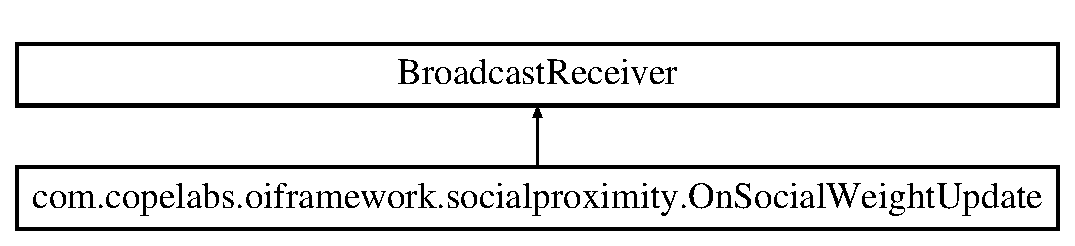
\includegraphics[height=2.000000cm]{classcom_1_1copelabs_1_1oiframework_1_1socialproximity_1_1_on_social_weight_update}
\end{center}
\end{figure}
\subsection*{Public Member Functions}
\begin{DoxyCompactItemize}
\item 
\hyperlink{classcom_1_1copelabs_1_1oiframework_1_1socialproximity_1_1_on_social_weight_update_a6d07da1e7f8c1551f442ef7aef7812e5}{On\+Social\+Weight\+Update} (\hyperlink{classcom_1_1copelabs_1_1oiframework_1_1socialproximity_1_1_data_base}{Data\+Base} database2, \hyperlink{classcom_1_1copelabs_1_1oiframework_1_1socialproximity_1_1_social_proximity}{Social\+Proximity} callback)
\item 
void \hyperlink{classcom_1_1copelabs_1_1oiframework_1_1socialproximity_1_1_on_social_weight_update_aa98a72b523b5b877ecce42ad1c7b324f}{on\+Receive} (Context context, Intent intent)
\item 
void \hyperlink{classcom_1_1copelabs_1_1oiframework_1_1socialproximity_1_1_on_social_weight_update_ae43a3aacd45e60256d75dcd113003a71}{compute\+Social\+Weight} (int sav\+Day, int curr\+Day, int curr\+Time\+Slot, long curr\+Time, boolean app\+R, boolean upd\+Over\+Diff\+Days)
\item 
int \hyperlink{classcom_1_1copelabs_1_1oiframework_1_1socialproximity_1_1_on_social_weight_update_a81d4d2ad2b4bc89781f672a32ab3d523}{get\+Time\+Slot} ()
\item 
void \hyperlink{classcom_1_1copelabs_1_1oiframework_1_1socialproximity_1_1_on_social_weight_update_a89365056e150cd1297ae3118edc6b6f8}{show\+Devices\+On\+D\+B} ()
\end{DoxyCompactItemize}
\subsection*{Static Public Attributes}
\begin{DoxyCompactItemize}
\item 
static int \hyperlink{classcom_1_1copelabs_1_1oiframework_1_1socialproximity_1_1_on_social_weight_update_a4f6cce6c6e893845f6f0db6d277e65dd}{day} = 1
\item 
static final String \hyperlink{classcom_1_1copelabs_1_1oiframework_1_1socialproximity_1_1_on_social_weight_update_afdd66acab94bdf2041f5b728d96df31d}{N\+E\+W\+\_\+\+H\+O\+U\+R}
\end{DoxyCompactItemize}
\subsection*{Private Member Functions}
\begin{DoxyCompactItemize}
\item 
void \hyperlink{classcom_1_1copelabs_1_1oiframework_1_1socialproximity_1_1_on_social_weight_update_a18178050f5ad0634bb905ca973b864ae}{notify\+Data\+Base\+Change} ()
\end{DoxyCompactItemize}
\subsection*{Private Attributes}
\begin{DoxyCompactItemize}
\item 
final String \hyperlink{classcom_1_1copelabs_1_1oiframework_1_1socialproximity_1_1_on_social_weight_update_a3bbf5341c4fb269f389aefe1e2ea7349}{T\+A\+G} = \char`\"{}Social Proximity\char`\"{}
\item 
\hyperlink{classcom_1_1copelabs_1_1oiframework_1_1socialproximity_1_1_data_base}{Data\+Base} \hyperlink{classcom_1_1copelabs_1_1oiframework_1_1socialproximity_1_1_on_social_weight_update_aebbc58a65323136459ba7d2bf34aca82}{database}
\item 
boolean \hyperlink{classcom_1_1copelabs_1_1oiframework_1_1socialproximity_1_1_on_social_weight_update_aba463f1549e47893cfeb042f75a82a89}{debug} = true
\item 
Array\+List$<$ \hyperlink{interfacecom_1_1copelabs_1_1oiframework_1_1socialproximity_1_1_data_base_change_listener}{Data\+Base\+Change\+Listener} $>$ \hyperlink{classcom_1_1copelabs_1_1oiframework_1_1socialproximity_1_1_on_social_weight_update_a8f80956e423a5d0548206be93870e412}{listeners} = new Array\+List$<$\hyperlink{interfacecom_1_1copelabs_1_1oiframework_1_1socialproximity_1_1_data_base_change_listener}{Data\+Base\+Change\+Listener}$>$ ()
\end{DoxyCompactItemize}


\subsection{Detailed Description}
\begin{DoxyVersion}{Version}
1.\+0 C\+O\+P\+Y\+R\+I\+G\+H\+T\+S C\+O\+P\+E\+L\+A\+B\+S/\+U\+L\+H\+T, L\+G\+P\+Lv3.\+0, 06-\/04-\/2016 Class is part of the S\+O\+C\+I\+O application. This class is responsible for computing the social weight among users. 
\end{DoxyVersion}
\begin{DoxyAuthor}{Author}
Waldir Moreira (C\+O\+P\+E\+L\+A\+B\+S/\+U\+L\+H\+T) 
\end{DoxyAuthor}


\subsection{Constructor \& Destructor Documentation}
\hypertarget{classcom_1_1copelabs_1_1oiframework_1_1socialproximity_1_1_on_social_weight_update_a6d07da1e7f8c1551f442ef7aef7812e5}{}\index{com\+::copelabs\+::oiframework\+::socialproximity\+::\+On\+Social\+Weight\+Update@{com\+::copelabs\+::oiframework\+::socialproximity\+::\+On\+Social\+Weight\+Update}!On\+Social\+Weight\+Update@{On\+Social\+Weight\+Update}}
\index{On\+Social\+Weight\+Update@{On\+Social\+Weight\+Update}!com\+::copelabs\+::oiframework\+::socialproximity\+::\+On\+Social\+Weight\+Update@{com\+::copelabs\+::oiframework\+::socialproximity\+::\+On\+Social\+Weight\+Update}}
\subsubsection[{On\+Social\+Weight\+Update(\+Data\+Base database2, Social\+Proximity callback)}]{\setlength{\rightskip}{0pt plus 5cm}com.\+copelabs.\+oiframework.\+socialproximity.\+On\+Social\+Weight\+Update.\+On\+Social\+Weight\+Update (
\begin{DoxyParamCaption}
\item[{{\bf Data\+Base}}]{database2, }
\item[{{\bf Social\+Proximity}}]{callback}
\end{DoxyParamCaption}
)}\label{classcom_1_1copelabs_1_1oiframework_1_1socialproximity_1_1_on_social_weight_update_a6d07da1e7f8c1551f442ef7aef7812e5}
This method is the constructor for \hyperlink{classcom_1_1copelabs_1_1oiframework_1_1socialproximity_1_1_on_social_weight_update}{On\+Social\+Weight\+Update}. 
\begin{DoxyParams}{Parameters}
{\em database2} & The database to be used. \\
\hline
{\em callback} & The \hyperlink{classcom_1_1copelabs_1_1oiframework_1_1socialproximity_1_1_social_proximity}{Social\+Proximity} object to allow notification on social weight changes. \\
\hline
\end{DoxyParams}


\subsection{Member Function Documentation}
\hypertarget{classcom_1_1copelabs_1_1oiframework_1_1socialproximity_1_1_on_social_weight_update_ae43a3aacd45e60256d75dcd113003a71}{}\index{com\+::copelabs\+::oiframework\+::socialproximity\+::\+On\+Social\+Weight\+Update@{com\+::copelabs\+::oiframework\+::socialproximity\+::\+On\+Social\+Weight\+Update}!compute\+Social\+Weight@{compute\+Social\+Weight}}
\index{compute\+Social\+Weight@{compute\+Social\+Weight}!com\+::copelabs\+::oiframework\+::socialproximity\+::\+On\+Social\+Weight\+Update@{com\+::copelabs\+::oiframework\+::socialproximity\+::\+On\+Social\+Weight\+Update}}
\subsubsection[{compute\+Social\+Weight(int sav\+Day, int curr\+Day, int curr\+Time\+Slot, long curr\+Time, boolean app\+R, boolean upd\+Over\+Diff\+Days)}]{\setlength{\rightskip}{0pt plus 5cm}void com.\+copelabs.\+oiframework.\+socialproximity.\+On\+Social\+Weight\+Update.\+compute\+Social\+Weight (
\begin{DoxyParamCaption}
\item[{int}]{sav\+Day, }
\item[{int}]{curr\+Day, }
\item[{int}]{curr\+Time\+Slot, }
\item[{long}]{curr\+Time, }
\item[{boolean}]{app\+R, }
\item[{boolean}]{upd\+Over\+Diff\+Days}
\end{DoxyParamCaption}
)}\label{classcom_1_1copelabs_1_1oiframework_1_1socialproximity_1_1_on_social_weight_update_ae43a3aacd45e60256d75dcd113003a71}
This method computes the social weight towards all encountered nodes 
\begin{DoxyParams}{Parameters}
{\em sav\+Day} & The day the app started running. \\
\hline
{\em curr\+Day} & The current day when the app restarted. \\
\hline
{\em curr\+Time\+Slot} & The current time slot when the app restarted. \\
\hline
{\em curr\+Time} & The current time when the app restarted. \\
\hline
{\em app\+R} & The flag that tells whether the app restarted. \\
\hline
{\em upd\+Over\+Diff\+Days} & The flag that indicates the updates occur over different days. \\
\hline
\end{DoxyParams}

\begin{DoxyItemize}
\item A negative value indicates the application restarted. 
\end{DoxyItemize}\hypertarget{classcom_1_1copelabs_1_1oiframework_1_1socialproximity_1_1_on_social_weight_update_a81d4d2ad2b4bc89781f672a32ab3d523}{}\index{com\+::copelabs\+::oiframework\+::socialproximity\+::\+On\+Social\+Weight\+Update@{com\+::copelabs\+::oiframework\+::socialproximity\+::\+On\+Social\+Weight\+Update}!get\+Time\+Slot@{get\+Time\+Slot}}
\index{get\+Time\+Slot@{get\+Time\+Slot}!com\+::copelabs\+::oiframework\+::socialproximity\+::\+On\+Social\+Weight\+Update@{com\+::copelabs\+::oiframework\+::socialproximity\+::\+On\+Social\+Weight\+Update}}
\subsubsection[{get\+Time\+Slot()}]{\setlength{\rightskip}{0pt plus 5cm}int com.\+copelabs.\+oiframework.\+socialproximity.\+On\+Social\+Weight\+Update.\+get\+Time\+Slot (
\begin{DoxyParamCaption}
{}
\end{DoxyParamCaption}
)}\label{classcom_1_1copelabs_1_1oiframework_1_1socialproximity_1_1_on_social_weight_update_a81d4d2ad2b4bc89781f672a32ab3d523}
This method provides the current time slot. \begin{DoxyReturn}{Returns}
current\+Time\+Slot The actual time slot. 
\end{DoxyReturn}
\hypertarget{classcom_1_1copelabs_1_1oiframework_1_1socialproximity_1_1_on_social_weight_update_a18178050f5ad0634bb905ca973b864ae}{}\index{com\+::copelabs\+::oiframework\+::socialproximity\+::\+On\+Social\+Weight\+Update@{com\+::copelabs\+::oiframework\+::socialproximity\+::\+On\+Social\+Weight\+Update}!notify\+Data\+Base\+Change@{notify\+Data\+Base\+Change}}
\index{notify\+Data\+Base\+Change@{notify\+Data\+Base\+Change}!com\+::copelabs\+::oiframework\+::socialproximity\+::\+On\+Social\+Weight\+Update@{com\+::copelabs\+::oiframework\+::socialproximity\+::\+On\+Social\+Weight\+Update}}
\subsubsection[{notify\+Data\+Base\+Change()}]{\setlength{\rightskip}{0pt plus 5cm}void com.\+copelabs.\+oiframework.\+socialproximity.\+On\+Social\+Weight\+Update.\+notify\+Data\+Base\+Change (
\begin{DoxyParamCaption}
{}
\end{DoxyParamCaption}
)\hspace{0.3cm}{\ttfamily [private]}}\label{classcom_1_1copelabs_1_1oiframework_1_1socialproximity_1_1_on_social_weight_update_a18178050f5ad0634bb905ca973b864ae}
This method notifies a database change to the listeners. \hypertarget{classcom_1_1copelabs_1_1oiframework_1_1socialproximity_1_1_on_social_weight_update_aa98a72b523b5b877ecce42ad1c7b324f}{}\index{com\+::copelabs\+::oiframework\+::socialproximity\+::\+On\+Social\+Weight\+Update@{com\+::copelabs\+::oiframework\+::socialproximity\+::\+On\+Social\+Weight\+Update}!on\+Receive@{on\+Receive}}
\index{on\+Receive@{on\+Receive}!com\+::copelabs\+::oiframework\+::socialproximity\+::\+On\+Social\+Weight\+Update@{com\+::copelabs\+::oiframework\+::socialproximity\+::\+On\+Social\+Weight\+Update}}
\subsubsection[{on\+Receive(\+Context context, Intent intent)}]{\setlength{\rightskip}{0pt plus 5cm}void com.\+copelabs.\+oiframework.\+socialproximity.\+On\+Social\+Weight\+Update.\+on\+Receive (
\begin{DoxyParamCaption}
\item[{Context}]{context, }
\item[{Intent}]{intent}
\end{DoxyParamCaption}
)}\label{classcom_1_1copelabs_1_1oiframework_1_1socialproximity_1_1_on_social_weight_update_aa98a72b523b5b877ecce42ad1c7b324f}
This method receives action concerning social weight updates. 
\begin{DoxyParams}{Parameters}
{\em context} & The context. \\
\hline
{\em intent} & The intent. \\
\hline
\end{DoxyParams}
\hypertarget{classcom_1_1copelabs_1_1oiframework_1_1socialproximity_1_1_on_social_weight_update_a89365056e150cd1297ae3118edc6b6f8}{}\index{com\+::copelabs\+::oiframework\+::socialproximity\+::\+On\+Social\+Weight\+Update@{com\+::copelabs\+::oiframework\+::socialproximity\+::\+On\+Social\+Weight\+Update}!show\+Devices\+On\+D\+B@{show\+Devices\+On\+D\+B}}
\index{show\+Devices\+On\+D\+B@{show\+Devices\+On\+D\+B}!com\+::copelabs\+::oiframework\+::socialproximity\+::\+On\+Social\+Weight\+Update@{com\+::copelabs\+::oiframework\+::socialproximity\+::\+On\+Social\+Weight\+Update}}
\subsubsection[{show\+Devices\+On\+D\+B()}]{\setlength{\rightskip}{0pt plus 5cm}void com.\+copelabs.\+oiframework.\+socialproximity.\+On\+Social\+Weight\+Update.\+show\+Devices\+On\+D\+B (
\begin{DoxyParamCaption}
{}
\end{DoxyParamCaption}
)}\label{classcom_1_1copelabs_1_1oiframework_1_1socialproximity_1_1_on_social_weight_update_a89365056e150cd1297ae3118edc6b6f8}
This method shows the Bluetooth devices stored on the D\+B. 

\subsection{Member Data Documentation}
\hypertarget{classcom_1_1copelabs_1_1oiframework_1_1socialproximity_1_1_on_social_weight_update_aebbc58a65323136459ba7d2bf34aca82}{}\index{com\+::copelabs\+::oiframework\+::socialproximity\+::\+On\+Social\+Weight\+Update@{com\+::copelabs\+::oiframework\+::socialproximity\+::\+On\+Social\+Weight\+Update}!database@{database}}
\index{database@{database}!com\+::copelabs\+::oiframework\+::socialproximity\+::\+On\+Social\+Weight\+Update@{com\+::copelabs\+::oiframework\+::socialproximity\+::\+On\+Social\+Weight\+Update}}
\subsubsection[{database}]{\setlength{\rightskip}{0pt plus 5cm}{\bf Data\+Base} com.\+copelabs.\+oiframework.\+socialproximity.\+On\+Social\+Weight\+Update.\+database\hspace{0.3cm}{\ttfamily [private]}}\label{classcom_1_1copelabs_1_1oiframework_1_1socialproximity_1_1_on_social_weight_update_aebbc58a65323136459ba7d2bf34aca82}
\hypertarget{classcom_1_1copelabs_1_1oiframework_1_1socialproximity_1_1_on_social_weight_update_a4f6cce6c6e893845f6f0db6d277e65dd}{}\index{com\+::copelabs\+::oiframework\+::socialproximity\+::\+On\+Social\+Weight\+Update@{com\+::copelabs\+::oiframework\+::socialproximity\+::\+On\+Social\+Weight\+Update}!day@{day}}
\index{day@{day}!com\+::copelabs\+::oiframework\+::socialproximity\+::\+On\+Social\+Weight\+Update@{com\+::copelabs\+::oiframework\+::socialproximity\+::\+On\+Social\+Weight\+Update}}
\subsubsection[{day}]{\setlength{\rightskip}{0pt plus 5cm}int com.\+copelabs.\+oiframework.\+socialproximity.\+On\+Social\+Weight\+Update.\+day = 1\hspace{0.3cm}{\ttfamily [static]}}\label{classcom_1_1copelabs_1_1oiframework_1_1socialproximity_1_1_on_social_weight_update_a4f6cce6c6e893845f6f0db6d277e65dd}
\hypertarget{classcom_1_1copelabs_1_1oiframework_1_1socialproximity_1_1_on_social_weight_update_aba463f1549e47893cfeb042f75a82a89}{}\index{com\+::copelabs\+::oiframework\+::socialproximity\+::\+On\+Social\+Weight\+Update@{com\+::copelabs\+::oiframework\+::socialproximity\+::\+On\+Social\+Weight\+Update}!debug@{debug}}
\index{debug@{debug}!com\+::copelabs\+::oiframework\+::socialproximity\+::\+On\+Social\+Weight\+Update@{com\+::copelabs\+::oiframework\+::socialproximity\+::\+On\+Social\+Weight\+Update}}
\subsubsection[{debug}]{\setlength{\rightskip}{0pt plus 5cm}boolean com.\+copelabs.\+oiframework.\+socialproximity.\+On\+Social\+Weight\+Update.\+debug = true\hspace{0.3cm}{\ttfamily [private]}}\label{classcom_1_1copelabs_1_1oiframework_1_1socialproximity_1_1_on_social_weight_update_aba463f1549e47893cfeb042f75a82a89}
\hypertarget{classcom_1_1copelabs_1_1oiframework_1_1socialproximity_1_1_on_social_weight_update_a8f80956e423a5d0548206be93870e412}{}\index{com\+::copelabs\+::oiframework\+::socialproximity\+::\+On\+Social\+Weight\+Update@{com\+::copelabs\+::oiframework\+::socialproximity\+::\+On\+Social\+Weight\+Update}!listeners@{listeners}}
\index{listeners@{listeners}!com\+::copelabs\+::oiframework\+::socialproximity\+::\+On\+Social\+Weight\+Update@{com\+::copelabs\+::oiframework\+::socialproximity\+::\+On\+Social\+Weight\+Update}}
\subsubsection[{listeners}]{\setlength{\rightskip}{0pt plus 5cm}Array\+List$<${\bf Data\+Base\+Change\+Listener}$>$ com.\+copelabs.\+oiframework.\+socialproximity.\+On\+Social\+Weight\+Update.\+listeners = new Array\+List$<${\bf Data\+Base\+Change\+Listener}$>$ ()\hspace{0.3cm}{\ttfamily [private]}}\label{classcom_1_1copelabs_1_1oiframework_1_1socialproximity_1_1_on_social_weight_update_a8f80956e423a5d0548206be93870e412}
\hypertarget{classcom_1_1copelabs_1_1oiframework_1_1socialproximity_1_1_on_social_weight_update_afdd66acab94bdf2041f5b728d96df31d}{}\index{com\+::copelabs\+::oiframework\+::socialproximity\+::\+On\+Social\+Weight\+Update@{com\+::copelabs\+::oiframework\+::socialproximity\+::\+On\+Social\+Weight\+Update}!N\+E\+W\+\_\+\+H\+O\+U\+R@{N\+E\+W\+\_\+\+H\+O\+U\+R}}
\index{N\+E\+W\+\_\+\+H\+O\+U\+R@{N\+E\+W\+\_\+\+H\+O\+U\+R}!com\+::copelabs\+::oiframework\+::socialproximity\+::\+On\+Social\+Weight\+Update@{com\+::copelabs\+::oiframework\+::socialproximity\+::\+On\+Social\+Weight\+Update}}
\subsubsection[{N\+E\+W\+\_\+\+H\+O\+U\+R}]{\setlength{\rightskip}{0pt plus 5cm}final String com.\+copelabs.\+oiframework.\+socialproximity.\+On\+Social\+Weight\+Update.\+N\+E\+W\+\_\+\+H\+O\+U\+R\hspace{0.3cm}{\ttfamily [static]}}\label{classcom_1_1copelabs_1_1oiframework_1_1socialproximity_1_1_on_social_weight_update_afdd66acab94bdf2041f5b728d96df31d}
{\bfseries Initial value\+:}
\begin{DoxyCode}
=
            \textcolor{stringliteral}{"android.intent.action.NEWHOUR"}
\end{DoxyCode}
\hypertarget{classcom_1_1copelabs_1_1oiframework_1_1socialproximity_1_1_on_social_weight_update_a3bbf5341c4fb269f389aefe1e2ea7349}{}\index{com\+::copelabs\+::oiframework\+::socialproximity\+::\+On\+Social\+Weight\+Update@{com\+::copelabs\+::oiframework\+::socialproximity\+::\+On\+Social\+Weight\+Update}!T\+A\+G@{T\+A\+G}}
\index{T\+A\+G@{T\+A\+G}!com\+::copelabs\+::oiframework\+::socialproximity\+::\+On\+Social\+Weight\+Update@{com\+::copelabs\+::oiframework\+::socialproximity\+::\+On\+Social\+Weight\+Update}}
\subsubsection[{T\+A\+G}]{\setlength{\rightskip}{0pt plus 5cm}final String com.\+copelabs.\+oiframework.\+socialproximity.\+On\+Social\+Weight\+Update.\+T\+A\+G = \char`\"{}Social Proximity\char`\"{}\hspace{0.3cm}{\ttfamily [private]}}\label{classcom_1_1copelabs_1_1oiframework_1_1socialproximity_1_1_on_social_weight_update_a3bbf5341c4fb269f389aefe1e2ea7349}


The documentation for this class was generated from the following file\+:\begin{DoxyCompactItemize}
\item 
src/com/copelabs/oiframework/socialproximity/\hyperlink{_on_social_weight_update_8java}{On\+Social\+Weight\+Update.\+java}\end{DoxyCompactItemize}

\hypertarget{classcom_1_1copelabs_1_1oiframework_1_1contentmanager_1_1_packet}{}\section{com.\+copelabs.\+oiframework.\+contentmanager.\+Packet Class Reference}
\label{classcom_1_1copelabs_1_1oiframework_1_1contentmanager_1_1_packet}\index{com.\+copelabs.\+oiframework.\+contentmanager.\+Packet@{com.\+copelabs.\+oiframework.\+contentmanager.\+Packet}}
Inheritance diagram for com.\+copelabs.\+oiframework.\+contentmanager.\+Packet\+:\begin{figure}[H]
\begin{center}
\leavevmode
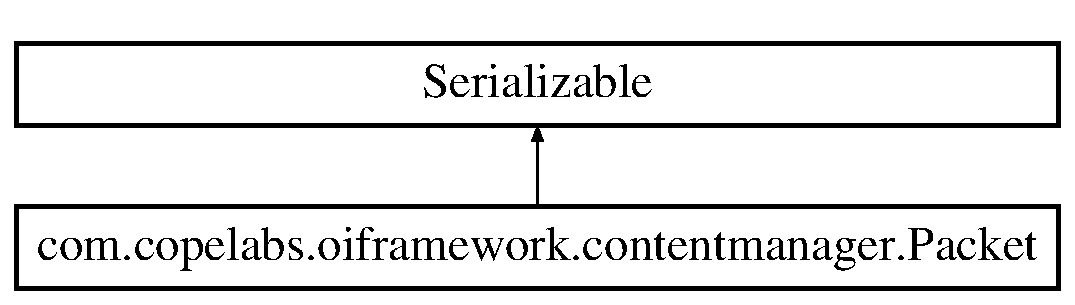
\includegraphics[height=2.000000cm]{classcom_1_1copelabs_1_1oiframework_1_1contentmanager_1_1_packet}
\end{center}
\end{figure}
\subsection*{Public Member Functions}
\begin{DoxyCompactItemize}
\item 
\hyperlink{classcom_1_1copelabs_1_1oiframework_1_1contentmanager_1_1_packet_a9b0e3e17127c15ba5ad44b4396113d0c}{Packet} ()
\item 
\hyperlink{classcom_1_1copelabs_1_1oiframework_1_1contentmanager_1_1_packet_a74503db32ef14429d932299a845a4c5f}{Packet} (String my\+B\+T\+M\+A\+C, String my\+B\+T\+Name)
\item 
String \hyperlink{classcom_1_1copelabs_1_1oiframework_1_1contentmanager_1_1_packet_acf75d58669cda28fa1d818de593d1eae}{get\+Id\+Source} ()
\item 
String \hyperlink{classcom_1_1copelabs_1_1oiframework_1_1contentmanager_1_1_packet_a567a7f33e7d0881b7b17cd062c1c914e}{get\+Id\+Destination} ()
\item 
String \hyperlink{classcom_1_1copelabs_1_1oiframework_1_1contentmanager_1_1_packet_adf672b7b0eb80a618d960a2be9cefc1d}{get\+Name\+Source} ()
\item 
String \hyperlink{classcom_1_1copelabs_1_1oiframework_1_1contentmanager_1_1_packet_acf4553b8748cabd0752afdaa0118339b}{get\+Name\+Destination} ()
\item 
String \hyperlink{classcom_1_1copelabs_1_1oiframework_1_1contentmanager_1_1_packet_a608fe53a0f1cf7db5f095c0f08d8cf0b}{get\+Application} ()
\item 
String \hyperlink{classcom_1_1copelabs_1_1oiframework_1_1contentmanager_1_1_packet_af294a6659b9b41a1d9fefedb39d214ee}{get\+Message} ()
\item 
long \hyperlink{classcom_1_1copelabs_1_1oiframework_1_1contentmanager_1_1_packet_adf3631e8d5d881eb635310aad9fceda6}{get\+Timestamp} ()
\item 
void \hyperlink{classcom_1_1copelabs_1_1oiframework_1_1contentmanager_1_1_packet_adbe1eedb580234ed8de7f670b90e6888}{set\+Id\+Source} (String \hyperlink{classcom_1_1copelabs_1_1oiframework_1_1contentmanager_1_1_packet_a68fee5247a550b8031b23b3f6bff6fca}{id\+Source})
\item 
void \hyperlink{classcom_1_1copelabs_1_1oiframework_1_1contentmanager_1_1_packet_a75e55f0f846942ada59fe2cdc02db0c7}{set\+Name\+Source} (String \hyperlink{classcom_1_1copelabs_1_1oiframework_1_1contentmanager_1_1_packet_ab73e6d976a992429142df8223a1be7e6}{name\+Source})
\item 
void \hyperlink{classcom_1_1copelabs_1_1oiframework_1_1contentmanager_1_1_packet_a3896a6e227b97e0a914dece9c828a245}{set\+Id\+Destination} (String \hyperlink{classcom_1_1copelabs_1_1oiframework_1_1contentmanager_1_1_packet_a2af44cf4979b64c494db4516b5038865}{id\+Destination})
\item 
void \hyperlink{classcom_1_1copelabs_1_1oiframework_1_1contentmanager_1_1_packet_a19a2660137b1d9f0db3812447b1cbe8b}{set\+Name\+Destination} (String \hyperlink{classcom_1_1copelabs_1_1oiframework_1_1contentmanager_1_1_packet_ae7e143efc19dd5eac86d39f69d366deb}{name\+Destination})
\item 
void \hyperlink{classcom_1_1copelabs_1_1oiframework_1_1contentmanager_1_1_packet_a8d58f5c3b30040078fdfab4b34c3ed34}{set\+Application} (String \hyperlink{classcom_1_1copelabs_1_1oiframework_1_1contentmanager_1_1_packet_aff42f5bf3f24dd4e271393fd23c30379}{application})
\item 
void \hyperlink{classcom_1_1copelabs_1_1oiframework_1_1contentmanager_1_1_packet_afebaf9b20497b91f16bb8f36f8386a48}{set\+Attributes} (String \hyperlink{classcom_1_1copelabs_1_1oiframework_1_1contentmanager_1_1_packet_a68fee5247a550b8031b23b3f6bff6fca}{id\+Source}, String \hyperlink{classcom_1_1copelabs_1_1oiframework_1_1contentmanager_1_1_packet_ab73e6d976a992429142df8223a1be7e6}{name\+Source}, String \hyperlink{classcom_1_1copelabs_1_1oiframework_1_1contentmanager_1_1_packet_a2af44cf4979b64c494db4516b5038865}{id\+Destination}, String \hyperlink{classcom_1_1copelabs_1_1oiframework_1_1contentmanager_1_1_packet_ae7e143efc19dd5eac86d39f69d366deb}{name\+Destination}, String \hyperlink{classcom_1_1copelabs_1_1oiframework_1_1contentmanager_1_1_packet_aff42f5bf3f24dd4e271393fd23c30379}{application}, String \hyperlink{classcom_1_1copelabs_1_1oiframework_1_1contentmanager_1_1_packet_a3fe10404c02da101b52018bf8c8b85f3}{message}, long \hyperlink{classcom_1_1copelabs_1_1oiframework_1_1contentmanager_1_1_packet_abc827d687f006831d6291505f0e31917}{timestamp})
\item 
void \hyperlink{classcom_1_1copelabs_1_1oiframework_1_1contentmanager_1_1_packet_a73e6d0f89eaaf555e1ad441304336c92}{set\+Message} (String msg)
\item 
void \hyperlink{classcom_1_1copelabs_1_1oiframework_1_1contentmanager_1_1_packet_ae23c6b6ae943fe5b50bbd3f57ebe409e}{set\+Timestamp} (long ts)
\item 
String \hyperlink{classcom_1_1copelabs_1_1oiframework_1_1contentmanager_1_1_packet_adf6b0b6c185796d731bea77f885f121e}{get\+Xml\+Entry} ()
\end{DoxyCompactItemize}
\subsection*{Static Public Attributes}
\begin{DoxyCompactItemize}
\item 
static final String \hyperlink{classcom_1_1copelabs_1_1oiframework_1_1contentmanager_1_1_packet_a6575deae949b07058159327b71e4c5d5}{T\+A\+G\+\_\+\+I\+D\+\_\+\+S\+O\+U\+R\+C\+E} = \char`\"{}id\+Source\char`\"{}
\item 
static final String \hyperlink{classcom_1_1copelabs_1_1oiframework_1_1contentmanager_1_1_packet_a120803d04db24e48fc40670e344a97f1}{T\+A\+G\+\_\+\+N\+A\+M\+E\+\_\+\+S\+O\+U\+R\+C\+E} = \char`\"{}name\+Source\char`\"{}
\item 
static final String \hyperlink{classcom_1_1copelabs_1_1oiframework_1_1contentmanager_1_1_packet_a1ed7f757f9bc5dc6d0a2d7915c0a8815}{T\+A\+G\+\_\+\+I\+D\+\_\+\+D\+E\+S\+T\+I\+N\+A\+T\+I\+O\+N} = \char`\"{}id\+Destination\char`\"{}
\item 
static final String \hyperlink{classcom_1_1copelabs_1_1oiframework_1_1contentmanager_1_1_packet_a7dad0fcae05780047e9c6c283923c4f5}{T\+A\+G\+\_\+\+N\+A\+M\+E\+\_\+\+D\+E\+S\+T\+I\+N\+A\+T\+I\+O\+N} = \char`\"{}name\+Destination\char`\"{}
\item 
static final String \hyperlink{classcom_1_1copelabs_1_1oiframework_1_1contentmanager_1_1_packet_a31017656446f4aea96409603e2135209}{T\+A\+G\+\_\+\+A\+P\+P\+L\+I\+C\+A\+T\+I\+O\+N} = \char`\"{}application\char`\"{}
\item 
static final String \hyperlink{classcom_1_1copelabs_1_1oiframework_1_1contentmanager_1_1_packet_a8b957cc44760ff9cf75aa5b84de87aa3}{T\+A\+G\+\_\+\+M\+E\+S\+S\+A\+G\+E} = \char`\"{}message\char`\"{}
\item 
static final String \hyperlink{classcom_1_1copelabs_1_1oiframework_1_1contentmanager_1_1_packet_a37f8b33849dc9655b171d2046905e6a2}{T\+A\+G\+\_\+\+T\+I\+M\+E\+S\+T\+A\+M\+P} = \char`\"{}timestamp\char`\"{}
\end{DoxyCompactItemize}
\subsection*{Private Attributes}
\begin{DoxyCompactItemize}
\item 
String \hyperlink{classcom_1_1copelabs_1_1oiframework_1_1contentmanager_1_1_packet_a68fee5247a550b8031b23b3f6bff6fca}{id\+Source}
\item 
String \hyperlink{classcom_1_1copelabs_1_1oiframework_1_1contentmanager_1_1_packet_ab73e6d976a992429142df8223a1be7e6}{name\+Source}
\item 
String \hyperlink{classcom_1_1copelabs_1_1oiframework_1_1contentmanager_1_1_packet_a2af44cf4979b64c494db4516b5038865}{id\+Destination}
\item 
String \hyperlink{classcom_1_1copelabs_1_1oiframework_1_1contentmanager_1_1_packet_ae7e143efc19dd5eac86d39f69d366deb}{name\+Destination}
\item 
String \hyperlink{classcom_1_1copelabs_1_1oiframework_1_1contentmanager_1_1_packet_aff42f5bf3f24dd4e271393fd23c30379}{application}
\item 
String \hyperlink{classcom_1_1copelabs_1_1oiframework_1_1contentmanager_1_1_packet_a3fe10404c02da101b52018bf8c8b85f3}{message} =\char`\"{}\char`\"{}
\item 
long \hyperlink{classcom_1_1copelabs_1_1oiframework_1_1contentmanager_1_1_packet_abc827d687f006831d6291505f0e31917}{timestamp}
\end{DoxyCompactItemize}
\subsection*{Static Private Attributes}
\begin{DoxyCompactItemize}
\item 
static final long \hyperlink{classcom_1_1copelabs_1_1oiframework_1_1contentmanager_1_1_packet_a3491d746da5c56128c2fe2ab5025cdd3}{serial\+Version\+U\+I\+D} = 1\+L
\end{DoxyCompactItemize}


\subsection{Detailed Description}

\begin{DoxyParams}{Parameters}
{\em id\+Source} & the identifier of the owner\textquotesingle{}s contact (B\+T M\+A\+C) \\
\hline
{\em name\+Source} & the name of the Sender contact (B\+T Name) \\
\hline
{\em id\+Destination} & the identifier of the selected contact (B\+T M\+A\+C) \\
\hline
{\em name\+Destination} & the name of the Receiver contact (B\+T Name) \\
\hline
{\em message} & the message content \\
\hline
{\em timestamp} & the timestamp for writing the message \\
\hline
\end{DoxyParams}


\subsection{Constructor \& Destructor Documentation}
\hypertarget{classcom_1_1copelabs_1_1oiframework_1_1contentmanager_1_1_packet_a9b0e3e17127c15ba5ad44b4396113d0c}{}\index{com\+::copelabs\+::oiframework\+::contentmanager\+::\+Packet@{com\+::copelabs\+::oiframework\+::contentmanager\+::\+Packet}!Packet@{Packet}}
\index{Packet@{Packet}!com\+::copelabs\+::oiframework\+::contentmanager\+::\+Packet@{com\+::copelabs\+::oiframework\+::contentmanager\+::\+Packet}}
\subsubsection[{Packet()}]{\setlength{\rightskip}{0pt plus 5cm}com.\+copelabs.\+oiframework.\+contentmanager.\+Packet.\+Packet (
\begin{DoxyParamCaption}
{}
\end{DoxyParamCaption}
)}\label{classcom_1_1copelabs_1_1oiframework_1_1contentmanager_1_1_packet_a9b0e3e17127c15ba5ad44b4396113d0c}
\hypertarget{classcom_1_1copelabs_1_1oiframework_1_1contentmanager_1_1_packet_a74503db32ef14429d932299a845a4c5f}{}\index{com\+::copelabs\+::oiframework\+::contentmanager\+::\+Packet@{com\+::copelabs\+::oiframework\+::contentmanager\+::\+Packet}!Packet@{Packet}}
\index{Packet@{Packet}!com\+::copelabs\+::oiframework\+::contentmanager\+::\+Packet@{com\+::copelabs\+::oiframework\+::contentmanager\+::\+Packet}}
\subsubsection[{Packet(\+String my\+B\+T\+M\+A\+C, String my\+B\+T\+Name)}]{\setlength{\rightskip}{0pt plus 5cm}com.\+copelabs.\+oiframework.\+contentmanager.\+Packet.\+Packet (
\begin{DoxyParamCaption}
\item[{String}]{my\+B\+T\+M\+A\+C, }
\item[{String}]{my\+B\+T\+Name}
\end{DoxyParamCaption}
)}\label{classcom_1_1copelabs_1_1oiframework_1_1contentmanager_1_1_packet_a74503db32ef14429d932299a845a4c5f}


\subsection{Member Function Documentation}
\hypertarget{classcom_1_1copelabs_1_1oiframework_1_1contentmanager_1_1_packet_a608fe53a0f1cf7db5f095c0f08d8cf0b}{}\index{com\+::copelabs\+::oiframework\+::contentmanager\+::\+Packet@{com\+::copelabs\+::oiframework\+::contentmanager\+::\+Packet}!get\+Application@{get\+Application}}
\index{get\+Application@{get\+Application}!com\+::copelabs\+::oiframework\+::contentmanager\+::\+Packet@{com\+::copelabs\+::oiframework\+::contentmanager\+::\+Packet}}
\subsubsection[{get\+Application()}]{\setlength{\rightskip}{0pt plus 5cm}String com.\+copelabs.\+oiframework.\+contentmanager.\+Packet.\+get\+Application (
\begin{DoxyParamCaption}
{}
\end{DoxyParamCaption}
)}\label{classcom_1_1copelabs_1_1oiframework_1_1contentmanager_1_1_packet_a608fe53a0f1cf7db5f095c0f08d8cf0b}
\hypertarget{classcom_1_1copelabs_1_1oiframework_1_1contentmanager_1_1_packet_a567a7f33e7d0881b7b17cd062c1c914e}{}\index{com\+::copelabs\+::oiframework\+::contentmanager\+::\+Packet@{com\+::copelabs\+::oiframework\+::contentmanager\+::\+Packet}!get\+Id\+Destination@{get\+Id\+Destination}}
\index{get\+Id\+Destination@{get\+Id\+Destination}!com\+::copelabs\+::oiframework\+::contentmanager\+::\+Packet@{com\+::copelabs\+::oiframework\+::contentmanager\+::\+Packet}}
\subsubsection[{get\+Id\+Destination()}]{\setlength{\rightskip}{0pt plus 5cm}String com.\+copelabs.\+oiframework.\+contentmanager.\+Packet.\+get\+Id\+Destination (
\begin{DoxyParamCaption}
{}
\end{DoxyParamCaption}
)}\label{classcom_1_1copelabs_1_1oiframework_1_1contentmanager_1_1_packet_a567a7f33e7d0881b7b17cd062c1c914e}
\hypertarget{classcom_1_1copelabs_1_1oiframework_1_1contentmanager_1_1_packet_acf75d58669cda28fa1d818de593d1eae}{}\index{com\+::copelabs\+::oiframework\+::contentmanager\+::\+Packet@{com\+::copelabs\+::oiframework\+::contentmanager\+::\+Packet}!get\+Id\+Source@{get\+Id\+Source}}
\index{get\+Id\+Source@{get\+Id\+Source}!com\+::copelabs\+::oiframework\+::contentmanager\+::\+Packet@{com\+::copelabs\+::oiframework\+::contentmanager\+::\+Packet}}
\subsubsection[{get\+Id\+Source()}]{\setlength{\rightskip}{0pt plus 5cm}String com.\+copelabs.\+oiframework.\+contentmanager.\+Packet.\+get\+Id\+Source (
\begin{DoxyParamCaption}
{}
\end{DoxyParamCaption}
)}\label{classcom_1_1copelabs_1_1oiframework_1_1contentmanager_1_1_packet_acf75d58669cda28fa1d818de593d1eae}
\hypertarget{classcom_1_1copelabs_1_1oiframework_1_1contentmanager_1_1_packet_af294a6659b9b41a1d9fefedb39d214ee}{}\index{com\+::copelabs\+::oiframework\+::contentmanager\+::\+Packet@{com\+::copelabs\+::oiframework\+::contentmanager\+::\+Packet}!get\+Message@{get\+Message}}
\index{get\+Message@{get\+Message}!com\+::copelabs\+::oiframework\+::contentmanager\+::\+Packet@{com\+::copelabs\+::oiframework\+::contentmanager\+::\+Packet}}
\subsubsection[{get\+Message()}]{\setlength{\rightskip}{0pt plus 5cm}String com.\+copelabs.\+oiframework.\+contentmanager.\+Packet.\+get\+Message (
\begin{DoxyParamCaption}
{}
\end{DoxyParamCaption}
)}\label{classcom_1_1copelabs_1_1oiframework_1_1contentmanager_1_1_packet_af294a6659b9b41a1d9fefedb39d214ee}
\hypertarget{classcom_1_1copelabs_1_1oiframework_1_1contentmanager_1_1_packet_acf4553b8748cabd0752afdaa0118339b}{}\index{com\+::copelabs\+::oiframework\+::contentmanager\+::\+Packet@{com\+::copelabs\+::oiframework\+::contentmanager\+::\+Packet}!get\+Name\+Destination@{get\+Name\+Destination}}
\index{get\+Name\+Destination@{get\+Name\+Destination}!com\+::copelabs\+::oiframework\+::contentmanager\+::\+Packet@{com\+::copelabs\+::oiframework\+::contentmanager\+::\+Packet}}
\subsubsection[{get\+Name\+Destination()}]{\setlength{\rightskip}{0pt plus 5cm}String com.\+copelabs.\+oiframework.\+contentmanager.\+Packet.\+get\+Name\+Destination (
\begin{DoxyParamCaption}
{}
\end{DoxyParamCaption}
)}\label{classcom_1_1copelabs_1_1oiframework_1_1contentmanager_1_1_packet_acf4553b8748cabd0752afdaa0118339b}
\hypertarget{classcom_1_1copelabs_1_1oiframework_1_1contentmanager_1_1_packet_adf672b7b0eb80a618d960a2be9cefc1d}{}\index{com\+::copelabs\+::oiframework\+::contentmanager\+::\+Packet@{com\+::copelabs\+::oiframework\+::contentmanager\+::\+Packet}!get\+Name\+Source@{get\+Name\+Source}}
\index{get\+Name\+Source@{get\+Name\+Source}!com\+::copelabs\+::oiframework\+::contentmanager\+::\+Packet@{com\+::copelabs\+::oiframework\+::contentmanager\+::\+Packet}}
\subsubsection[{get\+Name\+Source()}]{\setlength{\rightskip}{0pt plus 5cm}String com.\+copelabs.\+oiframework.\+contentmanager.\+Packet.\+get\+Name\+Source (
\begin{DoxyParamCaption}
{}
\end{DoxyParamCaption}
)}\label{classcom_1_1copelabs_1_1oiframework_1_1contentmanager_1_1_packet_adf672b7b0eb80a618d960a2be9cefc1d}
\hypertarget{classcom_1_1copelabs_1_1oiframework_1_1contentmanager_1_1_packet_adf3631e8d5d881eb635310aad9fceda6}{}\index{com\+::copelabs\+::oiframework\+::contentmanager\+::\+Packet@{com\+::copelabs\+::oiframework\+::contentmanager\+::\+Packet}!get\+Timestamp@{get\+Timestamp}}
\index{get\+Timestamp@{get\+Timestamp}!com\+::copelabs\+::oiframework\+::contentmanager\+::\+Packet@{com\+::copelabs\+::oiframework\+::contentmanager\+::\+Packet}}
\subsubsection[{get\+Timestamp()}]{\setlength{\rightskip}{0pt plus 5cm}long com.\+copelabs.\+oiframework.\+contentmanager.\+Packet.\+get\+Timestamp (
\begin{DoxyParamCaption}
{}
\end{DoxyParamCaption}
)}\label{classcom_1_1copelabs_1_1oiframework_1_1contentmanager_1_1_packet_adf3631e8d5d881eb635310aad9fceda6}
\hypertarget{classcom_1_1copelabs_1_1oiframework_1_1contentmanager_1_1_packet_adf6b0b6c185796d731bea77f885f121e}{}\index{com\+::copelabs\+::oiframework\+::contentmanager\+::\+Packet@{com\+::copelabs\+::oiframework\+::contentmanager\+::\+Packet}!get\+Xml\+Entry@{get\+Xml\+Entry}}
\index{get\+Xml\+Entry@{get\+Xml\+Entry}!com\+::copelabs\+::oiframework\+::contentmanager\+::\+Packet@{com\+::copelabs\+::oiframework\+::contentmanager\+::\+Packet}}
\subsubsection[{get\+Xml\+Entry()}]{\setlength{\rightskip}{0pt plus 5cm}String com.\+copelabs.\+oiframework.\+contentmanager.\+Packet.\+get\+Xml\+Entry (
\begin{DoxyParamCaption}
{}
\end{DoxyParamCaption}
)}\label{classcom_1_1copelabs_1_1oiframework_1_1contentmanager_1_1_packet_adf6b0b6c185796d731bea77f885f121e}
Writes an Oi\+Message (List) in xml format \begin{DoxyReturn}{Returns}
String an entry containing the xml format for an Oi\+Message 
\end{DoxyReturn}
\hypertarget{classcom_1_1copelabs_1_1oiframework_1_1contentmanager_1_1_packet_a8d58f5c3b30040078fdfab4b34c3ed34}{}\index{com\+::copelabs\+::oiframework\+::contentmanager\+::\+Packet@{com\+::copelabs\+::oiframework\+::contentmanager\+::\+Packet}!set\+Application@{set\+Application}}
\index{set\+Application@{set\+Application}!com\+::copelabs\+::oiframework\+::contentmanager\+::\+Packet@{com\+::copelabs\+::oiframework\+::contentmanager\+::\+Packet}}
\subsubsection[{set\+Application(\+String application)}]{\setlength{\rightskip}{0pt plus 5cm}void com.\+copelabs.\+oiframework.\+contentmanager.\+Packet.\+set\+Application (
\begin{DoxyParamCaption}
\item[{String}]{application}
\end{DoxyParamCaption}
)}\label{classcom_1_1copelabs_1_1oiframework_1_1contentmanager_1_1_packet_a8d58f5c3b30040078fdfab4b34c3ed34}
\hypertarget{classcom_1_1copelabs_1_1oiframework_1_1contentmanager_1_1_packet_afebaf9b20497b91f16bb8f36f8386a48}{}\index{com\+::copelabs\+::oiframework\+::contentmanager\+::\+Packet@{com\+::copelabs\+::oiframework\+::contentmanager\+::\+Packet}!set\+Attributes@{set\+Attributes}}
\index{set\+Attributes@{set\+Attributes}!com\+::copelabs\+::oiframework\+::contentmanager\+::\+Packet@{com\+::copelabs\+::oiframework\+::contentmanager\+::\+Packet}}
\subsubsection[{set\+Attributes(\+String id\+Source, String name\+Source, String id\+Destination, String name\+Destination, String application, String message, long timestamp)}]{\setlength{\rightskip}{0pt plus 5cm}void com.\+copelabs.\+oiframework.\+contentmanager.\+Packet.\+set\+Attributes (
\begin{DoxyParamCaption}
\item[{String}]{id\+Source, }
\item[{String}]{name\+Source, }
\item[{String}]{id\+Destination, }
\item[{String}]{name\+Destination, }
\item[{String}]{application, }
\item[{String}]{message, }
\item[{long}]{timestamp}
\end{DoxyParamCaption}
)}\label{classcom_1_1copelabs_1_1oiframework_1_1contentmanager_1_1_packet_afebaf9b20497b91f16bb8f36f8386a48}
\hypertarget{classcom_1_1copelabs_1_1oiframework_1_1contentmanager_1_1_packet_a3896a6e227b97e0a914dece9c828a245}{}\index{com\+::copelabs\+::oiframework\+::contentmanager\+::\+Packet@{com\+::copelabs\+::oiframework\+::contentmanager\+::\+Packet}!set\+Id\+Destination@{set\+Id\+Destination}}
\index{set\+Id\+Destination@{set\+Id\+Destination}!com\+::copelabs\+::oiframework\+::contentmanager\+::\+Packet@{com\+::copelabs\+::oiframework\+::contentmanager\+::\+Packet}}
\subsubsection[{set\+Id\+Destination(\+String id\+Destination)}]{\setlength{\rightskip}{0pt plus 5cm}void com.\+copelabs.\+oiframework.\+contentmanager.\+Packet.\+set\+Id\+Destination (
\begin{DoxyParamCaption}
\item[{String}]{id\+Destination}
\end{DoxyParamCaption}
)}\label{classcom_1_1copelabs_1_1oiframework_1_1contentmanager_1_1_packet_a3896a6e227b97e0a914dece9c828a245}
\hypertarget{classcom_1_1copelabs_1_1oiframework_1_1contentmanager_1_1_packet_adbe1eedb580234ed8de7f670b90e6888}{}\index{com\+::copelabs\+::oiframework\+::contentmanager\+::\+Packet@{com\+::copelabs\+::oiframework\+::contentmanager\+::\+Packet}!set\+Id\+Source@{set\+Id\+Source}}
\index{set\+Id\+Source@{set\+Id\+Source}!com\+::copelabs\+::oiframework\+::contentmanager\+::\+Packet@{com\+::copelabs\+::oiframework\+::contentmanager\+::\+Packet}}
\subsubsection[{set\+Id\+Source(\+String id\+Source)}]{\setlength{\rightskip}{0pt plus 5cm}void com.\+copelabs.\+oiframework.\+contentmanager.\+Packet.\+set\+Id\+Source (
\begin{DoxyParamCaption}
\item[{String}]{id\+Source}
\end{DoxyParamCaption}
)}\label{classcom_1_1copelabs_1_1oiframework_1_1contentmanager_1_1_packet_adbe1eedb580234ed8de7f670b90e6888}
\hypertarget{classcom_1_1copelabs_1_1oiframework_1_1contentmanager_1_1_packet_a73e6d0f89eaaf555e1ad441304336c92}{}\index{com\+::copelabs\+::oiframework\+::contentmanager\+::\+Packet@{com\+::copelabs\+::oiframework\+::contentmanager\+::\+Packet}!set\+Message@{set\+Message}}
\index{set\+Message@{set\+Message}!com\+::copelabs\+::oiframework\+::contentmanager\+::\+Packet@{com\+::copelabs\+::oiframework\+::contentmanager\+::\+Packet}}
\subsubsection[{set\+Message(\+String msg)}]{\setlength{\rightskip}{0pt plus 5cm}void com.\+copelabs.\+oiframework.\+contentmanager.\+Packet.\+set\+Message (
\begin{DoxyParamCaption}
\item[{String}]{msg}
\end{DoxyParamCaption}
)}\label{classcom_1_1copelabs_1_1oiframework_1_1contentmanager_1_1_packet_a73e6d0f89eaaf555e1ad441304336c92}
\hypertarget{classcom_1_1copelabs_1_1oiframework_1_1contentmanager_1_1_packet_a19a2660137b1d9f0db3812447b1cbe8b}{}\index{com\+::copelabs\+::oiframework\+::contentmanager\+::\+Packet@{com\+::copelabs\+::oiframework\+::contentmanager\+::\+Packet}!set\+Name\+Destination@{set\+Name\+Destination}}
\index{set\+Name\+Destination@{set\+Name\+Destination}!com\+::copelabs\+::oiframework\+::contentmanager\+::\+Packet@{com\+::copelabs\+::oiframework\+::contentmanager\+::\+Packet}}
\subsubsection[{set\+Name\+Destination(\+String name\+Destination)}]{\setlength{\rightskip}{0pt plus 5cm}void com.\+copelabs.\+oiframework.\+contentmanager.\+Packet.\+set\+Name\+Destination (
\begin{DoxyParamCaption}
\item[{String}]{name\+Destination}
\end{DoxyParamCaption}
)}\label{classcom_1_1copelabs_1_1oiframework_1_1contentmanager_1_1_packet_a19a2660137b1d9f0db3812447b1cbe8b}
\hypertarget{classcom_1_1copelabs_1_1oiframework_1_1contentmanager_1_1_packet_a75e55f0f846942ada59fe2cdc02db0c7}{}\index{com\+::copelabs\+::oiframework\+::contentmanager\+::\+Packet@{com\+::copelabs\+::oiframework\+::contentmanager\+::\+Packet}!set\+Name\+Source@{set\+Name\+Source}}
\index{set\+Name\+Source@{set\+Name\+Source}!com\+::copelabs\+::oiframework\+::contentmanager\+::\+Packet@{com\+::copelabs\+::oiframework\+::contentmanager\+::\+Packet}}
\subsubsection[{set\+Name\+Source(\+String name\+Source)}]{\setlength{\rightskip}{0pt plus 5cm}void com.\+copelabs.\+oiframework.\+contentmanager.\+Packet.\+set\+Name\+Source (
\begin{DoxyParamCaption}
\item[{String}]{name\+Source}
\end{DoxyParamCaption}
)}\label{classcom_1_1copelabs_1_1oiframework_1_1contentmanager_1_1_packet_a75e55f0f846942ada59fe2cdc02db0c7}
\hypertarget{classcom_1_1copelabs_1_1oiframework_1_1contentmanager_1_1_packet_ae23c6b6ae943fe5b50bbd3f57ebe409e}{}\index{com\+::copelabs\+::oiframework\+::contentmanager\+::\+Packet@{com\+::copelabs\+::oiframework\+::contentmanager\+::\+Packet}!set\+Timestamp@{set\+Timestamp}}
\index{set\+Timestamp@{set\+Timestamp}!com\+::copelabs\+::oiframework\+::contentmanager\+::\+Packet@{com\+::copelabs\+::oiframework\+::contentmanager\+::\+Packet}}
\subsubsection[{set\+Timestamp(long ts)}]{\setlength{\rightskip}{0pt plus 5cm}void com.\+copelabs.\+oiframework.\+contentmanager.\+Packet.\+set\+Timestamp (
\begin{DoxyParamCaption}
\item[{long}]{ts}
\end{DoxyParamCaption}
)}\label{classcom_1_1copelabs_1_1oiframework_1_1contentmanager_1_1_packet_ae23c6b6ae943fe5b50bbd3f57ebe409e}


\subsection{Member Data Documentation}
\hypertarget{classcom_1_1copelabs_1_1oiframework_1_1contentmanager_1_1_packet_aff42f5bf3f24dd4e271393fd23c30379}{}\index{com\+::copelabs\+::oiframework\+::contentmanager\+::\+Packet@{com\+::copelabs\+::oiframework\+::contentmanager\+::\+Packet}!application@{application}}
\index{application@{application}!com\+::copelabs\+::oiframework\+::contentmanager\+::\+Packet@{com\+::copelabs\+::oiframework\+::contentmanager\+::\+Packet}}
\subsubsection[{application}]{\setlength{\rightskip}{0pt plus 5cm}String com.\+copelabs.\+oiframework.\+contentmanager.\+Packet.\+application\hspace{0.3cm}{\ttfamily [private]}}\label{classcom_1_1copelabs_1_1oiframework_1_1contentmanager_1_1_packet_aff42f5bf3f24dd4e271393fd23c30379}
\hypertarget{classcom_1_1copelabs_1_1oiframework_1_1contentmanager_1_1_packet_a2af44cf4979b64c494db4516b5038865}{}\index{com\+::copelabs\+::oiframework\+::contentmanager\+::\+Packet@{com\+::copelabs\+::oiframework\+::contentmanager\+::\+Packet}!id\+Destination@{id\+Destination}}
\index{id\+Destination@{id\+Destination}!com\+::copelabs\+::oiframework\+::contentmanager\+::\+Packet@{com\+::copelabs\+::oiframework\+::contentmanager\+::\+Packet}}
\subsubsection[{id\+Destination}]{\setlength{\rightskip}{0pt plus 5cm}String com.\+copelabs.\+oiframework.\+contentmanager.\+Packet.\+id\+Destination\hspace{0.3cm}{\ttfamily [private]}}\label{classcom_1_1copelabs_1_1oiframework_1_1contentmanager_1_1_packet_a2af44cf4979b64c494db4516b5038865}
\hypertarget{classcom_1_1copelabs_1_1oiframework_1_1contentmanager_1_1_packet_a68fee5247a550b8031b23b3f6bff6fca}{}\index{com\+::copelabs\+::oiframework\+::contentmanager\+::\+Packet@{com\+::copelabs\+::oiframework\+::contentmanager\+::\+Packet}!id\+Source@{id\+Source}}
\index{id\+Source@{id\+Source}!com\+::copelabs\+::oiframework\+::contentmanager\+::\+Packet@{com\+::copelabs\+::oiframework\+::contentmanager\+::\+Packet}}
\subsubsection[{id\+Source}]{\setlength{\rightskip}{0pt plus 5cm}String com.\+copelabs.\+oiframework.\+contentmanager.\+Packet.\+id\+Source\hspace{0.3cm}{\ttfamily [private]}}\label{classcom_1_1copelabs_1_1oiframework_1_1contentmanager_1_1_packet_a68fee5247a550b8031b23b3f6bff6fca}
\hypertarget{classcom_1_1copelabs_1_1oiframework_1_1contentmanager_1_1_packet_a3fe10404c02da101b52018bf8c8b85f3}{}\index{com\+::copelabs\+::oiframework\+::contentmanager\+::\+Packet@{com\+::copelabs\+::oiframework\+::contentmanager\+::\+Packet}!message@{message}}
\index{message@{message}!com\+::copelabs\+::oiframework\+::contentmanager\+::\+Packet@{com\+::copelabs\+::oiframework\+::contentmanager\+::\+Packet}}
\subsubsection[{message}]{\setlength{\rightskip}{0pt plus 5cm}String com.\+copelabs.\+oiframework.\+contentmanager.\+Packet.\+message =\char`\"{}\char`\"{}\hspace{0.3cm}{\ttfamily [private]}}\label{classcom_1_1copelabs_1_1oiframework_1_1contentmanager_1_1_packet_a3fe10404c02da101b52018bf8c8b85f3}
\hypertarget{classcom_1_1copelabs_1_1oiframework_1_1contentmanager_1_1_packet_ae7e143efc19dd5eac86d39f69d366deb}{}\index{com\+::copelabs\+::oiframework\+::contentmanager\+::\+Packet@{com\+::copelabs\+::oiframework\+::contentmanager\+::\+Packet}!name\+Destination@{name\+Destination}}
\index{name\+Destination@{name\+Destination}!com\+::copelabs\+::oiframework\+::contentmanager\+::\+Packet@{com\+::copelabs\+::oiframework\+::contentmanager\+::\+Packet}}
\subsubsection[{name\+Destination}]{\setlength{\rightskip}{0pt plus 5cm}String com.\+copelabs.\+oiframework.\+contentmanager.\+Packet.\+name\+Destination\hspace{0.3cm}{\ttfamily [private]}}\label{classcom_1_1copelabs_1_1oiframework_1_1contentmanager_1_1_packet_ae7e143efc19dd5eac86d39f69d366deb}
\hypertarget{classcom_1_1copelabs_1_1oiframework_1_1contentmanager_1_1_packet_ab73e6d976a992429142df8223a1be7e6}{}\index{com\+::copelabs\+::oiframework\+::contentmanager\+::\+Packet@{com\+::copelabs\+::oiframework\+::contentmanager\+::\+Packet}!name\+Source@{name\+Source}}
\index{name\+Source@{name\+Source}!com\+::copelabs\+::oiframework\+::contentmanager\+::\+Packet@{com\+::copelabs\+::oiframework\+::contentmanager\+::\+Packet}}
\subsubsection[{name\+Source}]{\setlength{\rightskip}{0pt plus 5cm}String com.\+copelabs.\+oiframework.\+contentmanager.\+Packet.\+name\+Source\hspace{0.3cm}{\ttfamily [private]}}\label{classcom_1_1copelabs_1_1oiframework_1_1contentmanager_1_1_packet_ab73e6d976a992429142df8223a1be7e6}
\hypertarget{classcom_1_1copelabs_1_1oiframework_1_1contentmanager_1_1_packet_a3491d746da5c56128c2fe2ab5025cdd3}{}\index{com\+::copelabs\+::oiframework\+::contentmanager\+::\+Packet@{com\+::copelabs\+::oiframework\+::contentmanager\+::\+Packet}!serial\+Version\+U\+I\+D@{serial\+Version\+U\+I\+D}}
\index{serial\+Version\+U\+I\+D@{serial\+Version\+U\+I\+D}!com\+::copelabs\+::oiframework\+::contentmanager\+::\+Packet@{com\+::copelabs\+::oiframework\+::contentmanager\+::\+Packet}}
\subsubsection[{serial\+Version\+U\+I\+D}]{\setlength{\rightskip}{0pt plus 5cm}final long com.\+copelabs.\+oiframework.\+contentmanager.\+Packet.\+serial\+Version\+U\+I\+D = 1\+L\hspace{0.3cm}{\ttfamily [static]}, {\ttfamily [private]}}\label{classcom_1_1copelabs_1_1oiframework_1_1contentmanager_1_1_packet_a3491d746da5c56128c2fe2ab5025cdd3}
\hypertarget{classcom_1_1copelabs_1_1oiframework_1_1contentmanager_1_1_packet_a31017656446f4aea96409603e2135209}{}\index{com\+::copelabs\+::oiframework\+::contentmanager\+::\+Packet@{com\+::copelabs\+::oiframework\+::contentmanager\+::\+Packet}!T\+A\+G\+\_\+\+A\+P\+P\+L\+I\+C\+A\+T\+I\+O\+N@{T\+A\+G\+\_\+\+A\+P\+P\+L\+I\+C\+A\+T\+I\+O\+N}}
\index{T\+A\+G\+\_\+\+A\+P\+P\+L\+I\+C\+A\+T\+I\+O\+N@{T\+A\+G\+\_\+\+A\+P\+P\+L\+I\+C\+A\+T\+I\+O\+N}!com\+::copelabs\+::oiframework\+::contentmanager\+::\+Packet@{com\+::copelabs\+::oiframework\+::contentmanager\+::\+Packet}}
\subsubsection[{T\+A\+G\+\_\+\+A\+P\+P\+L\+I\+C\+A\+T\+I\+O\+N}]{\setlength{\rightskip}{0pt plus 5cm}final String com.\+copelabs.\+oiframework.\+contentmanager.\+Packet.\+T\+A\+G\+\_\+\+A\+P\+P\+L\+I\+C\+A\+T\+I\+O\+N = \char`\"{}application\char`\"{}\hspace{0.3cm}{\ttfamily [static]}}\label{classcom_1_1copelabs_1_1oiframework_1_1contentmanager_1_1_packet_a31017656446f4aea96409603e2135209}
\hypertarget{classcom_1_1copelabs_1_1oiframework_1_1contentmanager_1_1_packet_a1ed7f757f9bc5dc6d0a2d7915c0a8815}{}\index{com\+::copelabs\+::oiframework\+::contentmanager\+::\+Packet@{com\+::copelabs\+::oiframework\+::contentmanager\+::\+Packet}!T\+A\+G\+\_\+\+I\+D\+\_\+\+D\+E\+S\+T\+I\+N\+A\+T\+I\+O\+N@{T\+A\+G\+\_\+\+I\+D\+\_\+\+D\+E\+S\+T\+I\+N\+A\+T\+I\+O\+N}}
\index{T\+A\+G\+\_\+\+I\+D\+\_\+\+D\+E\+S\+T\+I\+N\+A\+T\+I\+O\+N@{T\+A\+G\+\_\+\+I\+D\+\_\+\+D\+E\+S\+T\+I\+N\+A\+T\+I\+O\+N}!com\+::copelabs\+::oiframework\+::contentmanager\+::\+Packet@{com\+::copelabs\+::oiframework\+::contentmanager\+::\+Packet}}
\subsubsection[{T\+A\+G\+\_\+\+I\+D\+\_\+\+D\+E\+S\+T\+I\+N\+A\+T\+I\+O\+N}]{\setlength{\rightskip}{0pt plus 5cm}final String com.\+copelabs.\+oiframework.\+contentmanager.\+Packet.\+T\+A\+G\+\_\+\+I\+D\+\_\+\+D\+E\+S\+T\+I\+N\+A\+T\+I\+O\+N = \char`\"{}id\+Destination\char`\"{}\hspace{0.3cm}{\ttfamily [static]}}\label{classcom_1_1copelabs_1_1oiframework_1_1contentmanager_1_1_packet_a1ed7f757f9bc5dc6d0a2d7915c0a8815}
\hypertarget{classcom_1_1copelabs_1_1oiframework_1_1contentmanager_1_1_packet_a6575deae949b07058159327b71e4c5d5}{}\index{com\+::copelabs\+::oiframework\+::contentmanager\+::\+Packet@{com\+::copelabs\+::oiframework\+::contentmanager\+::\+Packet}!T\+A\+G\+\_\+\+I\+D\+\_\+\+S\+O\+U\+R\+C\+E@{T\+A\+G\+\_\+\+I\+D\+\_\+\+S\+O\+U\+R\+C\+E}}
\index{T\+A\+G\+\_\+\+I\+D\+\_\+\+S\+O\+U\+R\+C\+E@{T\+A\+G\+\_\+\+I\+D\+\_\+\+S\+O\+U\+R\+C\+E}!com\+::copelabs\+::oiframework\+::contentmanager\+::\+Packet@{com\+::copelabs\+::oiframework\+::contentmanager\+::\+Packet}}
\subsubsection[{T\+A\+G\+\_\+\+I\+D\+\_\+\+S\+O\+U\+R\+C\+E}]{\setlength{\rightskip}{0pt plus 5cm}final String com.\+copelabs.\+oiframework.\+contentmanager.\+Packet.\+T\+A\+G\+\_\+\+I\+D\+\_\+\+S\+O\+U\+R\+C\+E = \char`\"{}id\+Source\char`\"{}\hspace{0.3cm}{\ttfamily [static]}}\label{classcom_1_1copelabs_1_1oiframework_1_1contentmanager_1_1_packet_a6575deae949b07058159327b71e4c5d5}
\hypertarget{classcom_1_1copelabs_1_1oiframework_1_1contentmanager_1_1_packet_a8b957cc44760ff9cf75aa5b84de87aa3}{}\index{com\+::copelabs\+::oiframework\+::contentmanager\+::\+Packet@{com\+::copelabs\+::oiframework\+::contentmanager\+::\+Packet}!T\+A\+G\+\_\+\+M\+E\+S\+S\+A\+G\+E@{T\+A\+G\+\_\+\+M\+E\+S\+S\+A\+G\+E}}
\index{T\+A\+G\+\_\+\+M\+E\+S\+S\+A\+G\+E@{T\+A\+G\+\_\+\+M\+E\+S\+S\+A\+G\+E}!com\+::copelabs\+::oiframework\+::contentmanager\+::\+Packet@{com\+::copelabs\+::oiframework\+::contentmanager\+::\+Packet}}
\subsubsection[{T\+A\+G\+\_\+\+M\+E\+S\+S\+A\+G\+E}]{\setlength{\rightskip}{0pt plus 5cm}final String com.\+copelabs.\+oiframework.\+contentmanager.\+Packet.\+T\+A\+G\+\_\+\+M\+E\+S\+S\+A\+G\+E = \char`\"{}message\char`\"{}\hspace{0.3cm}{\ttfamily [static]}}\label{classcom_1_1copelabs_1_1oiframework_1_1contentmanager_1_1_packet_a8b957cc44760ff9cf75aa5b84de87aa3}
\hypertarget{classcom_1_1copelabs_1_1oiframework_1_1contentmanager_1_1_packet_a7dad0fcae05780047e9c6c283923c4f5}{}\index{com\+::copelabs\+::oiframework\+::contentmanager\+::\+Packet@{com\+::copelabs\+::oiframework\+::contentmanager\+::\+Packet}!T\+A\+G\+\_\+\+N\+A\+M\+E\+\_\+\+D\+E\+S\+T\+I\+N\+A\+T\+I\+O\+N@{T\+A\+G\+\_\+\+N\+A\+M\+E\+\_\+\+D\+E\+S\+T\+I\+N\+A\+T\+I\+O\+N}}
\index{T\+A\+G\+\_\+\+N\+A\+M\+E\+\_\+\+D\+E\+S\+T\+I\+N\+A\+T\+I\+O\+N@{T\+A\+G\+\_\+\+N\+A\+M\+E\+\_\+\+D\+E\+S\+T\+I\+N\+A\+T\+I\+O\+N}!com\+::copelabs\+::oiframework\+::contentmanager\+::\+Packet@{com\+::copelabs\+::oiframework\+::contentmanager\+::\+Packet}}
\subsubsection[{T\+A\+G\+\_\+\+N\+A\+M\+E\+\_\+\+D\+E\+S\+T\+I\+N\+A\+T\+I\+O\+N}]{\setlength{\rightskip}{0pt plus 5cm}final String com.\+copelabs.\+oiframework.\+contentmanager.\+Packet.\+T\+A\+G\+\_\+\+N\+A\+M\+E\+\_\+\+D\+E\+S\+T\+I\+N\+A\+T\+I\+O\+N = \char`\"{}name\+Destination\char`\"{}\hspace{0.3cm}{\ttfamily [static]}}\label{classcom_1_1copelabs_1_1oiframework_1_1contentmanager_1_1_packet_a7dad0fcae05780047e9c6c283923c4f5}
\hypertarget{classcom_1_1copelabs_1_1oiframework_1_1contentmanager_1_1_packet_a120803d04db24e48fc40670e344a97f1}{}\index{com\+::copelabs\+::oiframework\+::contentmanager\+::\+Packet@{com\+::copelabs\+::oiframework\+::contentmanager\+::\+Packet}!T\+A\+G\+\_\+\+N\+A\+M\+E\+\_\+\+S\+O\+U\+R\+C\+E@{T\+A\+G\+\_\+\+N\+A\+M\+E\+\_\+\+S\+O\+U\+R\+C\+E}}
\index{T\+A\+G\+\_\+\+N\+A\+M\+E\+\_\+\+S\+O\+U\+R\+C\+E@{T\+A\+G\+\_\+\+N\+A\+M\+E\+\_\+\+S\+O\+U\+R\+C\+E}!com\+::copelabs\+::oiframework\+::contentmanager\+::\+Packet@{com\+::copelabs\+::oiframework\+::contentmanager\+::\+Packet}}
\subsubsection[{T\+A\+G\+\_\+\+N\+A\+M\+E\+\_\+\+S\+O\+U\+R\+C\+E}]{\setlength{\rightskip}{0pt plus 5cm}final String com.\+copelabs.\+oiframework.\+contentmanager.\+Packet.\+T\+A\+G\+\_\+\+N\+A\+M\+E\+\_\+\+S\+O\+U\+R\+C\+E = \char`\"{}name\+Source\char`\"{}\hspace{0.3cm}{\ttfamily [static]}}\label{classcom_1_1copelabs_1_1oiframework_1_1contentmanager_1_1_packet_a120803d04db24e48fc40670e344a97f1}
\hypertarget{classcom_1_1copelabs_1_1oiframework_1_1contentmanager_1_1_packet_a37f8b33849dc9655b171d2046905e6a2}{}\index{com\+::copelabs\+::oiframework\+::contentmanager\+::\+Packet@{com\+::copelabs\+::oiframework\+::contentmanager\+::\+Packet}!T\+A\+G\+\_\+\+T\+I\+M\+E\+S\+T\+A\+M\+P@{T\+A\+G\+\_\+\+T\+I\+M\+E\+S\+T\+A\+M\+P}}
\index{T\+A\+G\+\_\+\+T\+I\+M\+E\+S\+T\+A\+M\+P@{T\+A\+G\+\_\+\+T\+I\+M\+E\+S\+T\+A\+M\+P}!com\+::copelabs\+::oiframework\+::contentmanager\+::\+Packet@{com\+::copelabs\+::oiframework\+::contentmanager\+::\+Packet}}
\subsubsection[{T\+A\+G\+\_\+\+T\+I\+M\+E\+S\+T\+A\+M\+P}]{\setlength{\rightskip}{0pt plus 5cm}final String com.\+copelabs.\+oiframework.\+contentmanager.\+Packet.\+T\+A\+G\+\_\+\+T\+I\+M\+E\+S\+T\+A\+M\+P = \char`\"{}timestamp\char`\"{}\hspace{0.3cm}{\ttfamily [static]}}\label{classcom_1_1copelabs_1_1oiframework_1_1contentmanager_1_1_packet_a37f8b33849dc9655b171d2046905e6a2}
\hypertarget{classcom_1_1copelabs_1_1oiframework_1_1contentmanager_1_1_packet_abc827d687f006831d6291505f0e31917}{}\index{com\+::copelabs\+::oiframework\+::contentmanager\+::\+Packet@{com\+::copelabs\+::oiframework\+::contentmanager\+::\+Packet}!timestamp@{timestamp}}
\index{timestamp@{timestamp}!com\+::copelabs\+::oiframework\+::contentmanager\+::\+Packet@{com\+::copelabs\+::oiframework\+::contentmanager\+::\+Packet}}
\subsubsection[{timestamp}]{\setlength{\rightskip}{0pt plus 5cm}long com.\+copelabs.\+oiframework.\+contentmanager.\+Packet.\+timestamp\hspace{0.3cm}{\ttfamily [private]}}\label{classcom_1_1copelabs_1_1oiframework_1_1contentmanager_1_1_packet_abc827d687f006831d6291505f0e31917}


The documentation for this class was generated from the following file\+:\begin{DoxyCompactItemize}
\item 
src/com/copelabs/oiframework/contentmanager/\hyperlink{_packet_8java}{Packet.\+java}\end{DoxyCompactItemize}

\hypertarget{classcom_1_1copelabs_1_1oiframework_1_1router_1_1_routing}{}\section{com.\+copelabs.\+oiframework.\+router.\+Routing Class Reference}
\label{classcom_1_1copelabs_1_1oiframework_1_1router_1_1_routing}\index{com.\+copelabs.\+oiframework.\+router.\+Routing@{com.\+copelabs.\+oiframework.\+router.\+Routing}}
\subsection*{Public Member Functions}
\begin{DoxyCompactItemize}
\item 
\hyperlink{classcom_1_1copelabs_1_1oiframework_1_1router_1_1_routing_ae0f95c53f3cbd90db0dabba7dcc7cced}{Routing} (Context context)
\item 
List$<$ User\+Device $>$ \hyperlink{classcom_1_1copelabs_1_1oiframework_1_1router_1_1_routing_a477c2e1f830054864334dc96d08dc5e7}{get\+Contact\+List} ()
\item 
Map$<$ String, Integer $>$ \hyperlink{classcom_1_1copelabs_1_1oiframework_1_1router_1_1_routing_a9cb0fb0ced4521962b9c44bcb94d61bb}{get\+S\+W\+List} (Array\+List$<$ String $>$ m\+Devices)
\item 
Map$<$ String, Integer $>$ \hyperlink{classcom_1_1copelabs_1_1oiframework_1_1router_1_1_routing_affc739caaa3e1da2414ce75cd9af2433}{get\+All\+S\+W\+List} ()
\item 
List$<$ String $>$ \hyperlink{classcom_1_1copelabs_1_1oiframework_1_1router_1_1_routing_a9a667c08f302af1b2d3b8a934739505d}{get\+Local\+Info} ()
\item 
String \hyperlink{classcom_1_1copelabs_1_1oiframework_1_1router_1_1_routing_abb25bf0444ba72c9963a04cc7390fd7e}{get\+Local\+Mac\+Address} ()
\item 
String \hyperlink{classcom_1_1copelabs_1_1oiframework_1_1router_1_1_routing_ac2b1e57ed2b2a47b4cd44a80ddcf3ef7}{get\+Local\+Name} ()
\item 
void \hyperlink{classcom_1_1copelabs_1_1oiframework_1_1router_1_1_routing_ac888bfc58783ff88e2d59266c83d626e}{stop} ()
\item 
void \hyperlink{classcom_1_1copelabs_1_1oiframework_1_1router_1_1_routing_a226edc7be42ceb42c6a010685cdc7034}{set\+Routing\+Listener} (\hyperlink{interfacecom_1_1copelabs_1_1oiframework_1_1router_1_1_routing_listener}{Routing\+Listener} listener)
\item 
void \hyperlink{classcom_1_1copelabs_1_1oiframework_1_1router_1_1_routing_a0a869c067165f75ab986aea8f3befee6}{new\+Content\+Available} (\hyperlink{classcom_1_1copelabs_1_1oiframework_1_1contentmanager_1_1_packet}{Packet} m\+Packet)
\end{DoxyCompactItemize}
\subsection*{Public Attributes}
\begin{DoxyCompactItemize}
\item 
Array\+List$<$ \hyperlink{interfacecom_1_1copelabs_1_1oiframework_1_1router_1_1_routing_listener}{Routing\+Listener} $>$ \hyperlink{classcom_1_1copelabs_1_1oiframework_1_1router_1_1_routing_a7be56b16f52fd380dc20886c7b660878}{listeners} = new Array\+List$<$\hyperlink{interfacecom_1_1copelabs_1_1oiframework_1_1router_1_1_routing_listener}{Routing\+Listener}$>$ ()
\end{DoxyCompactItemize}
\subsection*{Static Public Attributes}
\begin{DoxyCompactItemize}
\item 
static final String \hyperlink{classcom_1_1copelabs_1_1oiframework_1_1router_1_1_routing_a49b371c77210ef1dd565cc7c9217b046}{T\+A\+G} =\char`\"{}Routing\char`\"{}
\end{DoxyCompactItemize}
\subsection*{Private Member Functions}
\begin{DoxyCompactItemize}
\item 
String \hyperlink{classcom_1_1copelabs_1_1oiframework_1_1router_1_1_routing_ae4f1793d12c6d079cf5b9881c3c37da8}{add\+Colon\+M\+A\+C} (String to\+Convert)
\item 
void \hyperlink{classcom_1_1copelabs_1_1oiframework_1_1router_1_1_routing_a858226e24ce2d6dd6c80579d59d4d32b}{announce\+List\+Social\+Weight} (Map$<$ String, Integer $>$ m\+List)
\item 
Map$<$ String, String $>$ \hyperlink{classcom_1_1copelabs_1_1oiframework_1_1router_1_1_routing_aea763e399345256b6992471ca927c4eb}{convert\+Map\+Value\+Double\+To\+String} (Map$<$ String, Integer $>$ map)
\item 
void \hyperlink{classcom_1_1copelabs_1_1oiframework_1_1router_1_1_routing_aa13558862a8cf3b097941b784cd81adc}{notify\+Packet\+Received} (List$<$ \hyperlink{classcom_1_1copelabs_1_1oiframework_1_1contentmanager_1_1_packet}{Packet} $>$ m\+List\+Of\+Packets)
\item 
Map$<$ String, List$<$ \hyperlink{classcom_1_1copelabs_1_1oiframework_1_1contentmanager_1_1_packet}{Packet} $>$ $>$ \hyperlink{classcom_1_1copelabs_1_1oiframework_1_1router_1_1_routing_a45f244e08d3e5e71c745c1517f14e419}{get\+List\+Of\+Packets} (List$<$ User\+Device $>$ m\+List\+Of\+User\+Devices)
\item 
void \hyperlink{classcom_1_1copelabs_1_1oiframework_1_1router_1_1_routing_acfb99144155277bff901572b3c574c38}{notify\+New\+Device\+Found} (User\+Device m\+User\+Device)
\item 
void \hyperlink{classcom_1_1copelabs_1_1oiframework_1_1router_1_1_routing_a537f880b57016bb88d8f806977c4b8af}{notify\+Device\+Disappear} (User\+Device m\+User\+Device)
\item 
void \hyperlink{classcom_1_1copelabs_1_1oiframework_1_1router_1_1_routing_a834835f4188adaa5f18fb428934d52b6}{notify\+Contact\+List\+Updated} (List$<$ User\+Device $>$ m\+List)
\item 
void \hyperlink{classcom_1_1copelabs_1_1oiframework_1_1router_1_1_routing_a2a7f53b5e97ec419cff6ff3022d60d70}{notify\+Error} (int m\+Error)
\end{DoxyCompactItemize}
\subsection*{Private Attributes}
\begin{DoxyCompactItemize}
\item 
\hyperlink{classcom_1_1copelabs_1_1oiframework_1_1socialproximity_1_1_social_proximity}{Social\+Proximity} \hyperlink{classcom_1_1copelabs_1_1oiframework_1_1router_1_1_routing_a2d75c4e7f78ea50811f94541832a64d1}{p\+Social\+Proximity}
\item 
\hyperlink{classcom_1_1copelabs_1_1oiframework_1_1wifi_1_1_wi_fi_direct}{Wi\+Fi\+Direct} \hyperlink{classcom_1_1copelabs_1_1oiframework_1_1router_1_1_routing_aa0ebfed6845783ed64cd90cce80d56e0}{p\+Wi\+Fi\+Direct}
\end{DoxyCompactItemize}


\subsection{Constructor \& Destructor Documentation}
\hypertarget{classcom_1_1copelabs_1_1oiframework_1_1router_1_1_routing_ae0f95c53f3cbd90db0dabba7dcc7cced}{}\index{com\+::copelabs\+::oiframework\+::router\+::\+Routing@{com\+::copelabs\+::oiframework\+::router\+::\+Routing}!Routing@{Routing}}
\index{Routing@{Routing}!com\+::copelabs\+::oiframework\+::router\+::\+Routing@{com\+::copelabs\+::oiframework\+::router\+::\+Routing}}
\subsubsection[{Routing(\+Context context)}]{\setlength{\rightskip}{0pt plus 5cm}com.\+copelabs.\+oiframework.\+router.\+Routing.\+Routing (
\begin{DoxyParamCaption}
\item[{Context}]{context}
\end{DoxyParamCaption}
)}\label{classcom_1_1copelabs_1_1oiframework_1_1router_1_1_routing_ae0f95c53f3cbd90db0dabba7dcc7cced}


\subsection{Member Function Documentation}
\hypertarget{classcom_1_1copelabs_1_1oiframework_1_1router_1_1_routing_ae4f1793d12c6d079cf5b9881c3c37da8}{}\index{com\+::copelabs\+::oiframework\+::router\+::\+Routing@{com\+::copelabs\+::oiframework\+::router\+::\+Routing}!add\+Colon\+M\+A\+C@{add\+Colon\+M\+A\+C}}
\index{add\+Colon\+M\+A\+C@{add\+Colon\+M\+A\+C}!com\+::copelabs\+::oiframework\+::router\+::\+Routing@{com\+::copelabs\+::oiframework\+::router\+::\+Routing}}
\subsubsection[{add\+Colon\+M\+A\+C(\+String to\+Convert)}]{\setlength{\rightskip}{0pt plus 5cm}String com.\+copelabs.\+oiframework.\+router.\+Routing.\+add\+Colon\+M\+A\+C (
\begin{DoxyParamCaption}
\item[{String}]{to\+Convert}
\end{DoxyParamCaption}
)\hspace{0.3cm}{\ttfamily [private]}}\label{classcom_1_1copelabs_1_1oiframework_1_1router_1_1_routing_ae4f1793d12c6d079cf5b9881c3c37da8}
\hypertarget{classcom_1_1copelabs_1_1oiframework_1_1router_1_1_routing_a858226e24ce2d6dd6c80579d59d4d32b}{}\index{com\+::copelabs\+::oiframework\+::router\+::\+Routing@{com\+::copelabs\+::oiframework\+::router\+::\+Routing}!announce\+List\+Social\+Weight@{announce\+List\+Social\+Weight}}
\index{announce\+List\+Social\+Weight@{announce\+List\+Social\+Weight}!com\+::copelabs\+::oiframework\+::router\+::\+Routing@{com\+::copelabs\+::oiframework\+::router\+::\+Routing}}
\subsubsection[{announce\+List\+Social\+Weight(\+Map$<$ String, Integer $>$ m\+List)}]{\setlength{\rightskip}{0pt plus 5cm}void com.\+copelabs.\+oiframework.\+router.\+Routing.\+announce\+List\+Social\+Weight (
\begin{DoxyParamCaption}
\item[{Map$<$ String, Integer $>$}]{m\+List}
\end{DoxyParamCaption}
)\hspace{0.3cm}{\ttfamily [private]}}\label{classcom_1_1copelabs_1_1oiframework_1_1router_1_1_routing_a858226e24ce2d6dd6c80579d59d4d32b}
\hypertarget{classcom_1_1copelabs_1_1oiframework_1_1router_1_1_routing_aea763e399345256b6992471ca927c4eb}{}\index{com\+::copelabs\+::oiframework\+::router\+::\+Routing@{com\+::copelabs\+::oiframework\+::router\+::\+Routing}!convert\+Map\+Value\+Double\+To\+String@{convert\+Map\+Value\+Double\+To\+String}}
\index{convert\+Map\+Value\+Double\+To\+String@{convert\+Map\+Value\+Double\+To\+String}!com\+::copelabs\+::oiframework\+::router\+::\+Routing@{com\+::copelabs\+::oiframework\+::router\+::\+Routing}}
\subsubsection[{convert\+Map\+Value\+Double\+To\+String(\+Map$<$ String, Integer $>$ map)}]{\setlength{\rightskip}{0pt plus 5cm}Map$<$String, String$>$ com.\+copelabs.\+oiframework.\+router.\+Routing.\+convert\+Map\+Value\+Double\+To\+String (
\begin{DoxyParamCaption}
\item[{Map$<$ String, Integer $>$}]{map}
\end{DoxyParamCaption}
)\hspace{0.3cm}{\ttfamily [private]}}\label{classcom_1_1copelabs_1_1oiframework_1_1router_1_1_routing_aea763e399345256b6992471ca927c4eb}
\hypertarget{classcom_1_1copelabs_1_1oiframework_1_1router_1_1_routing_affc739caaa3e1da2414ce75cd9af2433}{}\index{com\+::copelabs\+::oiframework\+::router\+::\+Routing@{com\+::copelabs\+::oiframework\+::router\+::\+Routing}!get\+All\+S\+W\+List@{get\+All\+S\+W\+List}}
\index{get\+All\+S\+W\+List@{get\+All\+S\+W\+List}!com\+::copelabs\+::oiframework\+::router\+::\+Routing@{com\+::copelabs\+::oiframework\+::router\+::\+Routing}}
\subsubsection[{get\+All\+S\+W\+List()}]{\setlength{\rightskip}{0pt plus 5cm}Map$<$String, Integer$>$ com.\+copelabs.\+oiframework.\+router.\+Routing.\+get\+All\+S\+W\+List (
\begin{DoxyParamCaption}
{}
\end{DoxyParamCaption}
)}\label{classcom_1_1copelabs_1_1oiframework_1_1router_1_1_routing_affc739caaa3e1da2414ce75cd9af2433}
Provides a list of all encountered devices and social weight towards them \begin{DoxyReturn}{Returns}
The list of all encountered devices and social weight towards them, or null 
\end{DoxyReturn}
\hypertarget{classcom_1_1copelabs_1_1oiframework_1_1router_1_1_routing_a477c2e1f830054864334dc96d08dc5e7}{}\index{com\+::copelabs\+::oiframework\+::router\+::\+Routing@{com\+::copelabs\+::oiframework\+::router\+::\+Routing}!get\+Contact\+List@{get\+Contact\+List}}
\index{get\+Contact\+List@{get\+Contact\+List}!com\+::copelabs\+::oiframework\+::router\+::\+Routing@{com\+::copelabs\+::oiframework\+::router\+::\+Routing}}
\subsubsection[{get\+Contact\+List()}]{\setlength{\rightskip}{0pt plus 5cm}List$<$User\+Device$>$ com.\+copelabs.\+oiframework.\+router.\+Routing.\+get\+Contact\+List (
\begin{DoxyParamCaption}
{}
\end{DoxyParamCaption}
)}\label{classcom_1_1copelabs_1_1oiframework_1_1router_1_1_routing_a477c2e1f830054864334dc96d08dc5e7}
Provides a list of contact based on the information of devices encountered \begin{DoxyReturn}{Returns}
The list of contacts or null 
\end{DoxyReturn}
\hypertarget{classcom_1_1copelabs_1_1oiframework_1_1router_1_1_routing_a45f244e08d3e5e71c745c1517f14e419}{}\index{com\+::copelabs\+::oiframework\+::router\+::\+Routing@{com\+::copelabs\+::oiframework\+::router\+::\+Routing}!get\+List\+Of\+Packets@{get\+List\+Of\+Packets}}
\index{get\+List\+Of\+Packets@{get\+List\+Of\+Packets}!com\+::copelabs\+::oiframework\+::router\+::\+Routing@{com\+::copelabs\+::oiframework\+::router\+::\+Routing}}
\subsubsection[{get\+List\+Of\+Packets(\+List$<$ User\+Device $>$ m\+List\+Of\+User\+Devices)}]{\setlength{\rightskip}{0pt plus 5cm}Map$<$String, List$<${\bf Packet}$>$ $>$ com.\+copelabs.\+oiframework.\+router.\+Routing.\+get\+List\+Of\+Packets (
\begin{DoxyParamCaption}
\item[{List$<$ User\+Device $>$}]{m\+List\+Of\+User\+Devices}
\end{DoxyParamCaption}
)\hspace{0.3cm}{\ttfamily [private]}}\label{classcom_1_1copelabs_1_1oiframework_1_1router_1_1_routing_a45f244e08d3e5e71c745c1517f14e419}
Provides a list of available packets to be sent to the given peers \begin{DoxyReturn}{Returns}
List of Packets available to send or null if Content Manager is not available. 
\end{DoxyReturn}
\hypertarget{classcom_1_1copelabs_1_1oiframework_1_1router_1_1_routing_a9a667c08f302af1b2d3b8a934739505d}{}\index{com\+::copelabs\+::oiframework\+::router\+::\+Routing@{com\+::copelabs\+::oiframework\+::router\+::\+Routing}!get\+Local\+Info@{get\+Local\+Info}}
\index{get\+Local\+Info@{get\+Local\+Info}!com\+::copelabs\+::oiframework\+::router\+::\+Routing@{com\+::copelabs\+::oiframework\+::router\+::\+Routing}}
\subsubsection[{get\+Local\+Info()}]{\setlength{\rightskip}{0pt plus 5cm}List$<$String$>$ com.\+copelabs.\+oiframework.\+router.\+Routing.\+get\+Local\+Info (
\begin{DoxyParamCaption}
{}
\end{DoxyParamCaption}
)}\label{classcom_1_1copelabs_1_1oiframework_1_1router_1_1_routing_a9a667c08f302af1b2d3b8a934739505d}
Provides the M\+A\+C Address of local Bluetooth adapter \begin{DoxyReturn}{Returns}
local\+Mac\+Add The local M\+A\+C Address or null 
\end{DoxyReturn}
\hypertarget{classcom_1_1copelabs_1_1oiframework_1_1router_1_1_routing_abb25bf0444ba72c9963a04cc7390fd7e}{}\index{com\+::copelabs\+::oiframework\+::router\+::\+Routing@{com\+::copelabs\+::oiframework\+::router\+::\+Routing}!get\+Local\+Mac\+Address@{get\+Local\+Mac\+Address}}
\index{get\+Local\+Mac\+Address@{get\+Local\+Mac\+Address}!com\+::copelabs\+::oiframework\+::router\+::\+Routing@{com\+::copelabs\+::oiframework\+::router\+::\+Routing}}
\subsubsection[{get\+Local\+Mac\+Address()}]{\setlength{\rightskip}{0pt plus 5cm}String com.\+copelabs.\+oiframework.\+router.\+Routing.\+get\+Local\+Mac\+Address (
\begin{DoxyParamCaption}
{}
\end{DoxyParamCaption}
)}\label{classcom_1_1copelabs_1_1oiframework_1_1router_1_1_routing_abb25bf0444ba72c9963a04cc7390fd7e}
\hypertarget{classcom_1_1copelabs_1_1oiframework_1_1router_1_1_routing_ac2b1e57ed2b2a47b4cd44a80ddcf3ef7}{}\index{com\+::copelabs\+::oiframework\+::router\+::\+Routing@{com\+::copelabs\+::oiframework\+::router\+::\+Routing}!get\+Local\+Name@{get\+Local\+Name}}
\index{get\+Local\+Name@{get\+Local\+Name}!com\+::copelabs\+::oiframework\+::router\+::\+Routing@{com\+::copelabs\+::oiframework\+::router\+::\+Routing}}
\subsubsection[{get\+Local\+Name()}]{\setlength{\rightskip}{0pt plus 5cm}String com.\+copelabs.\+oiframework.\+router.\+Routing.\+get\+Local\+Name (
\begin{DoxyParamCaption}
{}
\end{DoxyParamCaption}
)}\label{classcom_1_1copelabs_1_1oiframework_1_1router_1_1_routing_ac2b1e57ed2b2a47b4cd44a80ddcf3ef7}
\hypertarget{classcom_1_1copelabs_1_1oiframework_1_1router_1_1_routing_a9cb0fb0ced4521962b9c44bcb94d61bb}{}\index{com\+::copelabs\+::oiframework\+::router\+::\+Routing@{com\+::copelabs\+::oiframework\+::router\+::\+Routing}!get\+S\+W\+List@{get\+S\+W\+List}}
\index{get\+S\+W\+List@{get\+S\+W\+List}!com\+::copelabs\+::oiframework\+::router\+::\+Routing@{com\+::copelabs\+::oiframework\+::router\+::\+Routing}}
\subsubsection[{get\+S\+W\+List(\+Array\+List$<$ String $>$ m\+Devices)}]{\setlength{\rightskip}{0pt plus 5cm}Map$<$String, Integer$>$ com.\+copelabs.\+oiframework.\+router.\+Routing.\+get\+S\+W\+List (
\begin{DoxyParamCaption}
\item[{Array\+List$<$ String $>$}]{m\+Devices}
\end{DoxyParamCaption}
)}\label{classcom_1_1copelabs_1_1oiframework_1_1router_1_1_routing_a9cb0fb0ced4521962b9c44bcb94d61bb}
Provides a list of encountered devices and social weight towards them \begin{DoxyReturn}{Returns}
The list of encountered devices and social weight towards them, or null 
\end{DoxyReturn}
\hypertarget{classcom_1_1copelabs_1_1oiframework_1_1router_1_1_routing_a0a869c067165f75ab986aea8f3befee6}{}\index{com\+::copelabs\+::oiframework\+::router\+::\+Routing@{com\+::copelabs\+::oiframework\+::router\+::\+Routing}!new\+Content\+Available@{new\+Content\+Available}}
\index{new\+Content\+Available@{new\+Content\+Available}!com\+::copelabs\+::oiframework\+::router\+::\+Routing@{com\+::copelabs\+::oiframework\+::router\+::\+Routing}}
\subsubsection[{new\+Content\+Available(\+Packet m\+Packet)}]{\setlength{\rightskip}{0pt plus 5cm}void com.\+copelabs.\+oiframework.\+router.\+Routing.\+new\+Content\+Available (
\begin{DoxyParamCaption}
\item[{{\bf Packet}}]{m\+Packet}
\end{DoxyParamCaption}
)}\label{classcom_1_1copelabs_1_1oiframework_1_1router_1_1_routing_a0a869c067165f75ab986aea8f3befee6}
\hypertarget{classcom_1_1copelabs_1_1oiframework_1_1router_1_1_routing_a834835f4188adaa5f18fb428934d52b6}{}\index{com\+::copelabs\+::oiframework\+::router\+::\+Routing@{com\+::copelabs\+::oiframework\+::router\+::\+Routing}!notify\+Contact\+List\+Updated@{notify\+Contact\+List\+Updated}}
\index{notify\+Contact\+List\+Updated@{notify\+Contact\+List\+Updated}!com\+::copelabs\+::oiframework\+::router\+::\+Routing@{com\+::copelabs\+::oiframework\+::router\+::\+Routing}}
\subsubsection[{notify\+Contact\+List\+Updated(\+List$<$ User\+Device $>$ m\+List)}]{\setlength{\rightskip}{0pt plus 5cm}void com.\+copelabs.\+oiframework.\+router.\+Routing.\+notify\+Contact\+List\+Updated (
\begin{DoxyParamCaption}
\item[{List$<$ User\+Device $>$}]{m\+List}
\end{DoxyParamCaption}
)\hspace{0.3cm}{\ttfamily [private]}}\label{classcom_1_1copelabs_1_1oiframework_1_1router_1_1_routing_a834835f4188adaa5f18fb428934d52b6}
\hypertarget{classcom_1_1copelabs_1_1oiframework_1_1router_1_1_routing_a537f880b57016bb88d8f806977c4b8af}{}\index{com\+::copelabs\+::oiframework\+::router\+::\+Routing@{com\+::copelabs\+::oiframework\+::router\+::\+Routing}!notify\+Device\+Disappear@{notify\+Device\+Disappear}}
\index{notify\+Device\+Disappear@{notify\+Device\+Disappear}!com\+::copelabs\+::oiframework\+::router\+::\+Routing@{com\+::copelabs\+::oiframework\+::router\+::\+Routing}}
\subsubsection[{notify\+Device\+Disappear(\+User\+Device m\+User\+Device)}]{\setlength{\rightskip}{0pt plus 5cm}void com.\+copelabs.\+oiframework.\+router.\+Routing.\+notify\+Device\+Disappear (
\begin{DoxyParamCaption}
\item[{User\+Device}]{m\+User\+Device}
\end{DoxyParamCaption}
)\hspace{0.3cm}{\ttfamily [private]}}\label{classcom_1_1copelabs_1_1oiframework_1_1router_1_1_routing_a537f880b57016bb88d8f806977c4b8af}
\hypertarget{classcom_1_1copelabs_1_1oiframework_1_1router_1_1_routing_a2a7f53b5e97ec419cff6ff3022d60d70}{}\index{com\+::copelabs\+::oiframework\+::router\+::\+Routing@{com\+::copelabs\+::oiframework\+::router\+::\+Routing}!notify\+Error@{notify\+Error}}
\index{notify\+Error@{notify\+Error}!com\+::copelabs\+::oiframework\+::router\+::\+Routing@{com\+::copelabs\+::oiframework\+::router\+::\+Routing}}
\subsubsection[{notify\+Error(int m\+Error)}]{\setlength{\rightskip}{0pt plus 5cm}void com.\+copelabs.\+oiframework.\+router.\+Routing.\+notify\+Error (
\begin{DoxyParamCaption}
\item[{int}]{m\+Error}
\end{DoxyParamCaption}
)\hspace{0.3cm}{\ttfamily [private]}}\label{classcom_1_1copelabs_1_1oiframework_1_1router_1_1_routing_a2a7f53b5e97ec419cff6ff3022d60d70}
\hypertarget{classcom_1_1copelabs_1_1oiframework_1_1router_1_1_routing_acfb99144155277bff901572b3c574c38}{}\index{com\+::copelabs\+::oiframework\+::router\+::\+Routing@{com\+::copelabs\+::oiframework\+::router\+::\+Routing}!notify\+New\+Device\+Found@{notify\+New\+Device\+Found}}
\index{notify\+New\+Device\+Found@{notify\+New\+Device\+Found}!com\+::copelabs\+::oiframework\+::router\+::\+Routing@{com\+::copelabs\+::oiframework\+::router\+::\+Routing}}
\subsubsection[{notify\+New\+Device\+Found(\+User\+Device m\+User\+Device)}]{\setlength{\rightskip}{0pt plus 5cm}void com.\+copelabs.\+oiframework.\+router.\+Routing.\+notify\+New\+Device\+Found (
\begin{DoxyParamCaption}
\item[{User\+Device}]{m\+User\+Device}
\end{DoxyParamCaption}
)\hspace{0.3cm}{\ttfamily [private]}}\label{classcom_1_1copelabs_1_1oiframework_1_1router_1_1_routing_acfb99144155277bff901572b3c574c38}
\hypertarget{classcom_1_1copelabs_1_1oiframework_1_1router_1_1_routing_aa13558862a8cf3b097941b784cd81adc}{}\index{com\+::copelabs\+::oiframework\+::router\+::\+Routing@{com\+::copelabs\+::oiframework\+::router\+::\+Routing}!notify\+Packet\+Received@{notify\+Packet\+Received}}
\index{notify\+Packet\+Received@{notify\+Packet\+Received}!com\+::copelabs\+::oiframework\+::router\+::\+Routing@{com\+::copelabs\+::oiframework\+::router\+::\+Routing}}
\subsubsection[{notify\+Packet\+Received(\+List$<$ Packet $>$ m\+List\+Of\+Packets)}]{\setlength{\rightskip}{0pt plus 5cm}void com.\+copelabs.\+oiframework.\+router.\+Routing.\+notify\+Packet\+Received (
\begin{DoxyParamCaption}
\item[{List$<$ {\bf Packet} $>$}]{m\+List\+Of\+Packets}
\end{DoxyParamCaption}
)\hspace{0.3cm}{\ttfamily [private]}}\label{classcom_1_1copelabs_1_1oiframework_1_1router_1_1_routing_aa13558862a8cf3b097941b784cd81adc}
Notifies the Content\+Manager class that a new packet arrived. 
\begin{DoxyParams}{Parameters}
{\em m\+Packet} & Packet arrived \\
\hline
\end{DoxyParams}
\hypertarget{classcom_1_1copelabs_1_1oiframework_1_1router_1_1_routing_a226edc7be42ceb42c6a010685cdc7034}{}\index{com\+::copelabs\+::oiframework\+::router\+::\+Routing@{com\+::copelabs\+::oiframework\+::router\+::\+Routing}!set\+Routing\+Listener@{set\+Routing\+Listener}}
\index{set\+Routing\+Listener@{set\+Routing\+Listener}!com\+::copelabs\+::oiframework\+::router\+::\+Routing@{com\+::copelabs\+::oiframework\+::router\+::\+Routing}}
\subsubsection[{set\+Routing\+Listener(\+Routing\+Listener listener)}]{\setlength{\rightskip}{0pt plus 5cm}void com.\+copelabs.\+oiframework.\+router.\+Routing.\+set\+Routing\+Listener (
\begin{DoxyParamCaption}
\item[{{\bf Routing\+Listener}}]{listener}
\end{DoxyParamCaption}
)}\label{classcom_1_1copelabs_1_1oiframework_1_1router_1_1_routing_a226edc7be42ceb42c6a010685cdc7034}
\hypertarget{classcom_1_1copelabs_1_1oiframework_1_1router_1_1_routing_ac888bfc58783ff88e2d59266c83d626e}{}\index{com\+::copelabs\+::oiframework\+::router\+::\+Routing@{com\+::copelabs\+::oiframework\+::router\+::\+Routing}!stop@{stop}}
\index{stop@{stop}!com\+::copelabs\+::oiframework\+::router\+::\+Routing@{com\+::copelabs\+::oiframework\+::router\+::\+Routing}}
\subsubsection[{stop()}]{\setlength{\rightskip}{0pt plus 5cm}void com.\+copelabs.\+oiframework.\+router.\+Routing.\+stop (
\begin{DoxyParamCaption}
{}
\end{DoxyParamCaption}
)}\label{classcom_1_1copelabs_1_1oiframework_1_1router_1_1_routing_ac888bfc58783ff88e2d59266c83d626e}


\subsection{Member Data Documentation}
\hypertarget{classcom_1_1copelabs_1_1oiframework_1_1router_1_1_routing_a7be56b16f52fd380dc20886c7b660878}{}\index{com\+::copelabs\+::oiframework\+::router\+::\+Routing@{com\+::copelabs\+::oiframework\+::router\+::\+Routing}!listeners@{listeners}}
\index{listeners@{listeners}!com\+::copelabs\+::oiframework\+::router\+::\+Routing@{com\+::copelabs\+::oiframework\+::router\+::\+Routing}}
\subsubsection[{listeners}]{\setlength{\rightskip}{0pt plus 5cm}Array\+List$<${\bf Routing\+Listener}$>$ com.\+copelabs.\+oiframework.\+router.\+Routing.\+listeners = new Array\+List$<${\bf Routing\+Listener}$>$ ()}\label{classcom_1_1copelabs_1_1oiframework_1_1router_1_1_routing_a7be56b16f52fd380dc20886c7b660878}
\hypertarget{classcom_1_1copelabs_1_1oiframework_1_1router_1_1_routing_a2d75c4e7f78ea50811f94541832a64d1}{}\index{com\+::copelabs\+::oiframework\+::router\+::\+Routing@{com\+::copelabs\+::oiframework\+::router\+::\+Routing}!p\+Social\+Proximity@{p\+Social\+Proximity}}
\index{p\+Social\+Proximity@{p\+Social\+Proximity}!com\+::copelabs\+::oiframework\+::router\+::\+Routing@{com\+::copelabs\+::oiframework\+::router\+::\+Routing}}
\subsubsection[{p\+Social\+Proximity}]{\setlength{\rightskip}{0pt plus 5cm}{\bf Social\+Proximity} com.\+copelabs.\+oiframework.\+router.\+Routing.\+p\+Social\+Proximity\hspace{0.3cm}{\ttfamily [private]}}\label{classcom_1_1copelabs_1_1oiframework_1_1router_1_1_routing_a2d75c4e7f78ea50811f94541832a64d1}
\hypertarget{classcom_1_1copelabs_1_1oiframework_1_1router_1_1_routing_aa0ebfed6845783ed64cd90cce80d56e0}{}\index{com\+::copelabs\+::oiframework\+::router\+::\+Routing@{com\+::copelabs\+::oiframework\+::router\+::\+Routing}!p\+Wi\+Fi\+Direct@{p\+Wi\+Fi\+Direct}}
\index{p\+Wi\+Fi\+Direct@{p\+Wi\+Fi\+Direct}!com\+::copelabs\+::oiframework\+::router\+::\+Routing@{com\+::copelabs\+::oiframework\+::router\+::\+Routing}}
\subsubsection[{p\+Wi\+Fi\+Direct}]{\setlength{\rightskip}{0pt plus 5cm}{\bf Wi\+Fi\+Direct} com.\+copelabs.\+oiframework.\+router.\+Routing.\+p\+Wi\+Fi\+Direct\hspace{0.3cm}{\ttfamily [private]}}\label{classcom_1_1copelabs_1_1oiframework_1_1router_1_1_routing_aa0ebfed6845783ed64cd90cce80d56e0}
\hypertarget{classcom_1_1copelabs_1_1oiframework_1_1router_1_1_routing_a49b371c77210ef1dd565cc7c9217b046}{}\index{com\+::copelabs\+::oiframework\+::router\+::\+Routing@{com\+::copelabs\+::oiframework\+::router\+::\+Routing}!T\+A\+G@{T\+A\+G}}
\index{T\+A\+G@{T\+A\+G}!com\+::copelabs\+::oiframework\+::router\+::\+Routing@{com\+::copelabs\+::oiframework\+::router\+::\+Routing}}
\subsubsection[{T\+A\+G}]{\setlength{\rightskip}{0pt plus 5cm}final String com.\+copelabs.\+oiframework.\+router.\+Routing.\+T\+A\+G =\char`\"{}Routing\char`\"{}\hspace{0.3cm}{\ttfamily [static]}}\label{classcom_1_1copelabs_1_1oiframework_1_1router_1_1_routing_a49b371c77210ef1dd565cc7c9217b046}


The documentation for this class was generated from the following file\+:\begin{DoxyCompactItemize}
\item 
src/com/copelabs/oiframework/router/\hyperlink{_routing_8java}{Routing.\+java}\end{DoxyCompactItemize}

\hypertarget{interfacecom_1_1copelabs_1_1oiframework_1_1router_1_1_routing_listener}{}\section{com.\+copelabs.\+oiframework.\+router.\+Routing\+Listener Interface Reference}
\label{interfacecom_1_1copelabs_1_1oiframework_1_1router_1_1_routing_listener}\index{com.\+copelabs.\+oiframework.\+router.\+Routing\+Listener@{com.\+copelabs.\+oiframework.\+router.\+Routing\+Listener}}
\subsection*{Public Member Functions}
\begin{DoxyCompactItemize}
\item 
void \hyperlink{interfacecom_1_1copelabs_1_1oiframework_1_1router_1_1_routing_listener_a2f49c92e34e64a11caa4b37ced010947}{on\+Packet\+Received} (List$<$ \hyperlink{classcom_1_1copelabs_1_1oiframework_1_1contentmanager_1_1_packet}{Packet} $>$ m\+List\+Of\+Packets)
\item 
Map$<$ String, List$<$ \hyperlink{classcom_1_1copelabs_1_1oiframework_1_1contentmanager_1_1_packet}{Packet} $>$ $>$ \hyperlink{interfacecom_1_1copelabs_1_1oiframework_1_1router_1_1_routing_listener_aae99454a61f8e1e1a18049f8c4a8fcf2}{get\+List\+Of\+Packets} (List$<$ User\+Device $>$ m\+List\+Of\+User\+Devices)
\item 
void \hyperlink{interfacecom_1_1copelabs_1_1oiframework_1_1router_1_1_routing_listener_a0c81da81d2671a6391f9d0bd19fa6358}{new\+Device\+Found} (User\+Device m\+Device)
\item 
void \hyperlink{interfacecom_1_1copelabs_1_1oiframework_1_1router_1_1_routing_listener_a572b1fd128461739748b038086fa411d}{device\+Lost} (User\+Device m\+Device)
\item 
void \hyperlink{interfacecom_1_1copelabs_1_1oiframework_1_1router_1_1_routing_listener_aa98938a27b5e9efe5be1f4309e008302}{contact\+List\+Updated} (List$<$ User\+Device $>$ m\+List\+Of\+Packets)
\item 
void \hyperlink{interfacecom_1_1copelabs_1_1oiframework_1_1router_1_1_routing_listener_a03309a95f954512e20d607a2a3beb614}{error} (int m\+Error)
\end{DoxyCompactItemize}


\subsection{Member Function Documentation}
\hypertarget{interfacecom_1_1copelabs_1_1oiframework_1_1router_1_1_routing_listener_aa98938a27b5e9efe5be1f4309e008302}{}\index{com\+::copelabs\+::oiframework\+::router\+::\+Routing\+Listener@{com\+::copelabs\+::oiframework\+::router\+::\+Routing\+Listener}!contact\+List\+Updated@{contact\+List\+Updated}}
\index{contact\+List\+Updated@{contact\+List\+Updated}!com\+::copelabs\+::oiframework\+::router\+::\+Routing\+Listener@{com\+::copelabs\+::oiframework\+::router\+::\+Routing\+Listener}}
\subsubsection[{contact\+List\+Updated(\+List$<$ User\+Device $>$ m\+List\+Of\+Packets)}]{\setlength{\rightskip}{0pt plus 5cm}void com.\+copelabs.\+oiframework.\+router.\+Routing\+Listener.\+contact\+List\+Updated (
\begin{DoxyParamCaption}
\item[{List$<$ User\+Device $>$}]{m\+List\+Of\+Packets}
\end{DoxyParamCaption}
)}\label{interfacecom_1_1copelabs_1_1oiframework_1_1router_1_1_routing_listener_aa98938a27b5e9efe5be1f4309e008302}
\hypertarget{interfacecom_1_1copelabs_1_1oiframework_1_1router_1_1_routing_listener_a572b1fd128461739748b038086fa411d}{}\index{com\+::copelabs\+::oiframework\+::router\+::\+Routing\+Listener@{com\+::copelabs\+::oiframework\+::router\+::\+Routing\+Listener}!device\+Lost@{device\+Lost}}
\index{device\+Lost@{device\+Lost}!com\+::copelabs\+::oiframework\+::router\+::\+Routing\+Listener@{com\+::copelabs\+::oiframework\+::router\+::\+Routing\+Listener}}
\subsubsection[{device\+Lost(\+User\+Device m\+Device)}]{\setlength{\rightskip}{0pt plus 5cm}void com.\+copelabs.\+oiframework.\+router.\+Routing\+Listener.\+device\+Lost (
\begin{DoxyParamCaption}
\item[{User\+Device}]{m\+Device}
\end{DoxyParamCaption}
)}\label{interfacecom_1_1copelabs_1_1oiframework_1_1router_1_1_routing_listener_a572b1fd128461739748b038086fa411d}
\hypertarget{interfacecom_1_1copelabs_1_1oiframework_1_1router_1_1_routing_listener_a03309a95f954512e20d607a2a3beb614}{}\index{com\+::copelabs\+::oiframework\+::router\+::\+Routing\+Listener@{com\+::copelabs\+::oiframework\+::router\+::\+Routing\+Listener}!error@{error}}
\index{error@{error}!com\+::copelabs\+::oiframework\+::router\+::\+Routing\+Listener@{com\+::copelabs\+::oiframework\+::router\+::\+Routing\+Listener}}
\subsubsection[{error(int m\+Error)}]{\setlength{\rightskip}{0pt plus 5cm}void com.\+copelabs.\+oiframework.\+router.\+Routing\+Listener.\+error (
\begin{DoxyParamCaption}
\item[{int}]{m\+Error}
\end{DoxyParamCaption}
)}\label{interfacecom_1_1copelabs_1_1oiframework_1_1router_1_1_routing_listener_a03309a95f954512e20d607a2a3beb614}
\hypertarget{interfacecom_1_1copelabs_1_1oiframework_1_1router_1_1_routing_listener_aae99454a61f8e1e1a18049f8c4a8fcf2}{}\index{com\+::copelabs\+::oiframework\+::router\+::\+Routing\+Listener@{com\+::copelabs\+::oiframework\+::router\+::\+Routing\+Listener}!get\+List\+Of\+Packets@{get\+List\+Of\+Packets}}
\index{get\+List\+Of\+Packets@{get\+List\+Of\+Packets}!com\+::copelabs\+::oiframework\+::router\+::\+Routing\+Listener@{com\+::copelabs\+::oiframework\+::router\+::\+Routing\+Listener}}
\subsubsection[{get\+List\+Of\+Packets(\+List$<$ User\+Device $>$ m\+List\+Of\+User\+Devices)}]{\setlength{\rightskip}{0pt plus 5cm}Map$<$String, List$<${\bf Packet}$>$ $>$ com.\+copelabs.\+oiframework.\+router.\+Routing\+Listener.\+get\+List\+Of\+Packets (
\begin{DoxyParamCaption}
\item[{List$<$ User\+Device $>$}]{m\+List\+Of\+User\+Devices}
\end{DoxyParamCaption}
)}\label{interfacecom_1_1copelabs_1_1oiframework_1_1router_1_1_routing_listener_aae99454a61f8e1e1a18049f8c4a8fcf2}
\hypertarget{interfacecom_1_1copelabs_1_1oiframework_1_1router_1_1_routing_listener_a0c81da81d2671a6391f9d0bd19fa6358}{}\index{com\+::copelabs\+::oiframework\+::router\+::\+Routing\+Listener@{com\+::copelabs\+::oiframework\+::router\+::\+Routing\+Listener}!new\+Device\+Found@{new\+Device\+Found}}
\index{new\+Device\+Found@{new\+Device\+Found}!com\+::copelabs\+::oiframework\+::router\+::\+Routing\+Listener@{com\+::copelabs\+::oiframework\+::router\+::\+Routing\+Listener}}
\subsubsection[{new\+Device\+Found(\+User\+Device m\+Device)}]{\setlength{\rightskip}{0pt plus 5cm}void com.\+copelabs.\+oiframework.\+router.\+Routing\+Listener.\+new\+Device\+Found (
\begin{DoxyParamCaption}
\item[{User\+Device}]{m\+Device}
\end{DoxyParamCaption}
)}\label{interfacecom_1_1copelabs_1_1oiframework_1_1router_1_1_routing_listener_a0c81da81d2671a6391f9d0bd19fa6358}
\hypertarget{interfacecom_1_1copelabs_1_1oiframework_1_1router_1_1_routing_listener_a2f49c92e34e64a11caa4b37ced010947}{}\index{com\+::copelabs\+::oiframework\+::router\+::\+Routing\+Listener@{com\+::copelabs\+::oiframework\+::router\+::\+Routing\+Listener}!on\+Packet\+Received@{on\+Packet\+Received}}
\index{on\+Packet\+Received@{on\+Packet\+Received}!com\+::copelabs\+::oiframework\+::router\+::\+Routing\+Listener@{com\+::copelabs\+::oiframework\+::router\+::\+Routing\+Listener}}
\subsubsection[{on\+Packet\+Received(\+List$<$ Packet $>$ m\+List\+Of\+Packets)}]{\setlength{\rightskip}{0pt plus 5cm}void com.\+copelabs.\+oiframework.\+router.\+Routing\+Listener.\+on\+Packet\+Received (
\begin{DoxyParamCaption}
\item[{List$<$ {\bf Packet} $>$}]{m\+List\+Of\+Packets}
\end{DoxyParamCaption}
)}\label{interfacecom_1_1copelabs_1_1oiframework_1_1router_1_1_routing_listener_a2f49c92e34e64a11caa4b37ced010947}


The documentation for this interface was generated from the following file\+:\begin{DoxyCompactItemize}
\item 
src/com/copelabs/oiframework/router/\hyperlink{_routing_listener_8java}{Routing\+Listener.\+java}\end{DoxyCompactItemize}

\hypertarget{classcom_1_1copelabs_1_1oiframework_1_1wifi_1_1_send_data}{}\section{com.\+copelabs.\+oiframework.\+wifi.\+Send\+Data Class Reference}
\label{classcom_1_1copelabs_1_1oiframework_1_1wifi_1_1_send_data}\index{com.\+copelabs.\+oiframework.\+wifi.\+Send\+Data@{com.\+copelabs.\+oiframework.\+wifi.\+Send\+Data}}
Inheritance diagram for com.\+copelabs.\+oiframework.\+wifi.\+Send\+Data\+:\begin{figure}[H]
\begin{center}
\leavevmode
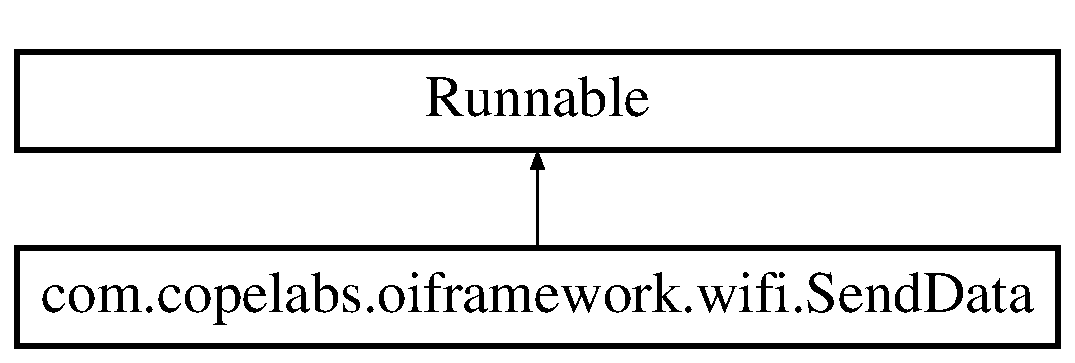
\includegraphics[height=2.000000cm]{classcom_1_1copelabs_1_1oiframework_1_1wifi_1_1_send_data}
\end{center}
\end{figure}
\subsection*{Public Member Functions}
\begin{DoxyCompactItemize}
\item 
\hyperlink{classcom_1_1copelabs_1_1oiframework_1_1wifi_1_1_send_data_a7313916aaed78662aae8b001a40868d7}{Send\+Data} (Socket \hyperlink{classcom_1_1copelabs_1_1oiframework_1_1wifi_1_1_send_data_aa68cb225ef22bd5e5b057320c8a28c0e}{socket}, Handler \hyperlink{classcom_1_1copelabs_1_1oiframework_1_1wifi_1_1_send_data_a21513ac56025f0efe9e80a1f6b087c2d}{handler})
\item 
void \hyperlink{classcom_1_1copelabs_1_1oiframework_1_1wifi_1_1_send_data_ab7d4fa2454e67ae279a7da9a750b688a}{run} ()
\item 
void \hyperlink{classcom_1_1copelabs_1_1oiframework_1_1wifi_1_1_send_data_a8ecc2a21ec4fd523e962987651be8df9}{write} (byte\mbox{[}$\,$\mbox{]} buffer)
\end{DoxyCompactItemize}
\subsection*{Private Attributes}
\begin{DoxyCompactItemize}
\item 
Socket \hyperlink{classcom_1_1copelabs_1_1oiframework_1_1wifi_1_1_send_data_aa68cb225ef22bd5e5b057320c8a28c0e}{socket} = null
\item 
Handler \hyperlink{classcom_1_1copelabs_1_1oiframework_1_1wifi_1_1_send_data_a21513ac56025f0efe9e80a1f6b087c2d}{handler}
\item 
Input\+Stream \hyperlink{classcom_1_1copelabs_1_1oiframework_1_1wifi_1_1_send_data_aeb2f33e45f684cac0cde3495ddac0a15}{i\+Stream}
\item 
Output\+Stream \hyperlink{classcom_1_1copelabs_1_1oiframework_1_1wifi_1_1_send_data_aa2e24df043ee09164380f1dc9fc20812}{o\+Stream}
\end{DoxyCompactItemize}
\subsection*{Static Private Attributes}
\begin{DoxyCompactItemize}
\item 
static final String \hyperlink{classcom_1_1copelabs_1_1oiframework_1_1wifi_1_1_send_data_a07d7509ad0cd62acbc46c1e85602ac1e}{T\+A\+G} = \char`\"{}Chat\+Handler\char`\"{}
\end{DoxyCompactItemize}


\subsection{Detailed Description}
Handles reading and writing of messages with socket buffers. Uses a Handler to post messages to U\+I thread for U\+I updates. 

\subsection{Constructor \& Destructor Documentation}
\hypertarget{classcom_1_1copelabs_1_1oiframework_1_1wifi_1_1_send_data_a7313916aaed78662aae8b001a40868d7}{}\index{com\+::copelabs\+::oiframework\+::wifi\+::\+Send\+Data@{com\+::copelabs\+::oiframework\+::wifi\+::\+Send\+Data}!Send\+Data@{Send\+Data}}
\index{Send\+Data@{Send\+Data}!com\+::copelabs\+::oiframework\+::wifi\+::\+Send\+Data@{com\+::copelabs\+::oiframework\+::wifi\+::\+Send\+Data}}
\subsubsection[{Send\+Data(\+Socket socket, Handler handler)}]{\setlength{\rightskip}{0pt plus 5cm}com.\+copelabs.\+oiframework.\+wifi.\+Send\+Data.\+Send\+Data (
\begin{DoxyParamCaption}
\item[{Socket}]{socket, }
\item[{Handler}]{handler}
\end{DoxyParamCaption}
)}\label{classcom_1_1copelabs_1_1oiframework_1_1wifi_1_1_send_data_a7313916aaed78662aae8b001a40868d7}


\subsection{Member Function Documentation}
\hypertarget{classcom_1_1copelabs_1_1oiframework_1_1wifi_1_1_send_data_ab7d4fa2454e67ae279a7da9a750b688a}{}\index{com\+::copelabs\+::oiframework\+::wifi\+::\+Send\+Data@{com\+::copelabs\+::oiframework\+::wifi\+::\+Send\+Data}!run@{run}}
\index{run@{run}!com\+::copelabs\+::oiframework\+::wifi\+::\+Send\+Data@{com\+::copelabs\+::oiframework\+::wifi\+::\+Send\+Data}}
\subsubsection[{run()}]{\setlength{\rightskip}{0pt plus 5cm}void com.\+copelabs.\+oiframework.\+wifi.\+Send\+Data.\+run (
\begin{DoxyParamCaption}
{}
\end{DoxyParamCaption}
)}\label{classcom_1_1copelabs_1_1oiframework_1_1wifi_1_1_send_data_ab7d4fa2454e67ae279a7da9a750b688a}
\hypertarget{classcom_1_1copelabs_1_1oiframework_1_1wifi_1_1_send_data_a8ecc2a21ec4fd523e962987651be8df9}{}\index{com\+::copelabs\+::oiframework\+::wifi\+::\+Send\+Data@{com\+::copelabs\+::oiframework\+::wifi\+::\+Send\+Data}!write@{write}}
\index{write@{write}!com\+::copelabs\+::oiframework\+::wifi\+::\+Send\+Data@{com\+::copelabs\+::oiframework\+::wifi\+::\+Send\+Data}}
\subsubsection[{write(byte[] buffer)}]{\setlength{\rightskip}{0pt plus 5cm}void com.\+copelabs.\+oiframework.\+wifi.\+Send\+Data.\+write (
\begin{DoxyParamCaption}
\item[{byte\mbox{[}$\,$\mbox{]}}]{buffer}
\end{DoxyParamCaption}
)}\label{classcom_1_1copelabs_1_1oiframework_1_1wifi_1_1_send_data_a8ecc2a21ec4fd523e962987651be8df9}


\subsection{Member Data Documentation}
\hypertarget{classcom_1_1copelabs_1_1oiframework_1_1wifi_1_1_send_data_a21513ac56025f0efe9e80a1f6b087c2d}{}\index{com\+::copelabs\+::oiframework\+::wifi\+::\+Send\+Data@{com\+::copelabs\+::oiframework\+::wifi\+::\+Send\+Data}!handler@{handler}}
\index{handler@{handler}!com\+::copelabs\+::oiframework\+::wifi\+::\+Send\+Data@{com\+::copelabs\+::oiframework\+::wifi\+::\+Send\+Data}}
\subsubsection[{handler}]{\setlength{\rightskip}{0pt plus 5cm}Handler com.\+copelabs.\+oiframework.\+wifi.\+Send\+Data.\+handler\hspace{0.3cm}{\ttfamily [private]}}\label{classcom_1_1copelabs_1_1oiframework_1_1wifi_1_1_send_data_a21513ac56025f0efe9e80a1f6b087c2d}
\hypertarget{classcom_1_1copelabs_1_1oiframework_1_1wifi_1_1_send_data_aeb2f33e45f684cac0cde3495ddac0a15}{}\index{com\+::copelabs\+::oiframework\+::wifi\+::\+Send\+Data@{com\+::copelabs\+::oiframework\+::wifi\+::\+Send\+Data}!i\+Stream@{i\+Stream}}
\index{i\+Stream@{i\+Stream}!com\+::copelabs\+::oiframework\+::wifi\+::\+Send\+Data@{com\+::copelabs\+::oiframework\+::wifi\+::\+Send\+Data}}
\subsubsection[{i\+Stream}]{\setlength{\rightskip}{0pt plus 5cm}Input\+Stream com.\+copelabs.\+oiframework.\+wifi.\+Send\+Data.\+i\+Stream\hspace{0.3cm}{\ttfamily [private]}}\label{classcom_1_1copelabs_1_1oiframework_1_1wifi_1_1_send_data_aeb2f33e45f684cac0cde3495ddac0a15}
\hypertarget{classcom_1_1copelabs_1_1oiframework_1_1wifi_1_1_send_data_aa2e24df043ee09164380f1dc9fc20812}{}\index{com\+::copelabs\+::oiframework\+::wifi\+::\+Send\+Data@{com\+::copelabs\+::oiframework\+::wifi\+::\+Send\+Data}!o\+Stream@{o\+Stream}}
\index{o\+Stream@{o\+Stream}!com\+::copelabs\+::oiframework\+::wifi\+::\+Send\+Data@{com\+::copelabs\+::oiframework\+::wifi\+::\+Send\+Data}}
\subsubsection[{o\+Stream}]{\setlength{\rightskip}{0pt plus 5cm}Output\+Stream com.\+copelabs.\+oiframework.\+wifi.\+Send\+Data.\+o\+Stream\hspace{0.3cm}{\ttfamily [private]}}\label{classcom_1_1copelabs_1_1oiframework_1_1wifi_1_1_send_data_aa2e24df043ee09164380f1dc9fc20812}
\hypertarget{classcom_1_1copelabs_1_1oiframework_1_1wifi_1_1_send_data_aa68cb225ef22bd5e5b057320c8a28c0e}{}\index{com\+::copelabs\+::oiframework\+::wifi\+::\+Send\+Data@{com\+::copelabs\+::oiframework\+::wifi\+::\+Send\+Data}!socket@{socket}}
\index{socket@{socket}!com\+::copelabs\+::oiframework\+::wifi\+::\+Send\+Data@{com\+::copelabs\+::oiframework\+::wifi\+::\+Send\+Data}}
\subsubsection[{socket}]{\setlength{\rightskip}{0pt plus 5cm}Socket com.\+copelabs.\+oiframework.\+wifi.\+Send\+Data.\+socket = null\hspace{0.3cm}{\ttfamily [private]}}\label{classcom_1_1copelabs_1_1oiframework_1_1wifi_1_1_send_data_aa68cb225ef22bd5e5b057320c8a28c0e}
\hypertarget{classcom_1_1copelabs_1_1oiframework_1_1wifi_1_1_send_data_a07d7509ad0cd62acbc46c1e85602ac1e}{}\index{com\+::copelabs\+::oiframework\+::wifi\+::\+Send\+Data@{com\+::copelabs\+::oiframework\+::wifi\+::\+Send\+Data}!T\+A\+G@{T\+A\+G}}
\index{T\+A\+G@{T\+A\+G}!com\+::copelabs\+::oiframework\+::wifi\+::\+Send\+Data@{com\+::copelabs\+::oiframework\+::wifi\+::\+Send\+Data}}
\subsubsection[{T\+A\+G}]{\setlength{\rightskip}{0pt plus 5cm}final String com.\+copelabs.\+oiframework.\+wifi.\+Send\+Data.\+T\+A\+G = \char`\"{}Chat\+Handler\char`\"{}\hspace{0.3cm}{\ttfamily [static]}, {\ttfamily [private]}}\label{classcom_1_1copelabs_1_1oiframework_1_1wifi_1_1_send_data_a07d7509ad0cd62acbc46c1e85602ac1e}


The documentation for this class was generated from the following file\+:\begin{DoxyCompactItemize}
\item 
src/com/copelabs/oiframework/wifi/\hyperlink{_send_data_8java}{Send\+Data.\+java}\end{DoxyCompactItemize}

\hypertarget{classcom_1_1copelabs_1_1oiframework_1_1wifi_1_1_server_thread}{}\section{com.\+copelabs.\+oiframework.\+wifi.\+Server\+Thread Class Reference}
\label{classcom_1_1copelabs_1_1oiframework_1_1wifi_1_1_server_thread}\index{com.\+copelabs.\+oiframework.\+wifi.\+Server\+Thread@{com.\+copelabs.\+oiframework.\+wifi.\+Server\+Thread}}
Inheritance diagram for com.\+copelabs.\+oiframework.\+wifi.\+Server\+Thread\+:\begin{figure}[H]
\begin{center}
\leavevmode
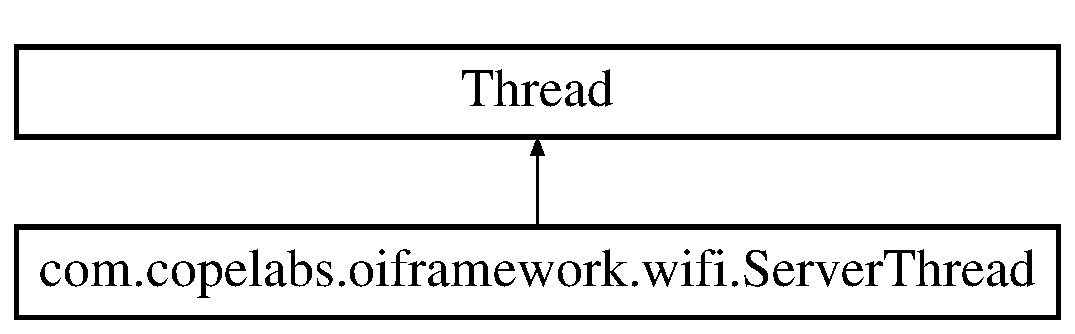
\includegraphics[height=2.000000cm]{classcom_1_1copelabs_1_1oiframework_1_1wifi_1_1_server_thread}
\end{center}
\end{figure}
\subsection*{Public Member Functions}
\begin{DoxyCompactItemize}
\item 
\hyperlink{classcom_1_1copelabs_1_1oiframework_1_1wifi_1_1_server_thread_a2b707824c7757ea46feba5f1b2188859}{Server\+Thread} (Handler \hyperlink{classcom_1_1copelabs_1_1oiframework_1_1wifi_1_1_server_thread_a6407a46f8c994464afa1782d2a7155ce}{handler}, Map$<$ String, List$<$ \hyperlink{classcom_1_1copelabs_1_1oiframework_1_1contentmanager_1_1_packet}{Packet} $>$$>$ \hyperlink{classcom_1_1copelabs_1_1oiframework_1_1wifi_1_1_server_thread_a8e8d2255357f62b00ab191fe1cdd9007}{m\+To\+Send})  throws I\+O\+Exception 
\item 
void \hyperlink{classcom_1_1copelabs_1_1oiframework_1_1wifi_1_1_server_thread_a62aa791f633ca2826de8d3c846197397}{run} ()
\end{DoxyCompactItemize}
\subsection*{Static Public Attributes}
\begin{DoxyCompactItemize}
\item 
static final int \hyperlink{classcom_1_1copelabs_1_1oiframework_1_1wifi_1_1_server_thread_aeafee844e7748efce835f579ec272782}{S\+E\+R\+V\+E\+R\+\_\+\+P\+O\+R\+T} = 4545
\end{DoxyCompactItemize}
\subsection*{Private Attributes}
\begin{DoxyCompactItemize}
\item 
final int \hyperlink{classcom_1_1copelabs_1_1oiframework_1_1wifi_1_1_server_thread_ab8508790f80a8cd728096ea45dab519f}{T\+H\+R\+E\+A\+D\+\_\+\+C\+O\+U\+N\+T} = 10
\item 
Handler \hyperlink{classcom_1_1copelabs_1_1oiframework_1_1wifi_1_1_server_thread_a6407a46f8c994464afa1782d2a7155ce}{handler}
\item 
Map$<$ String, List$<$ \hyperlink{classcom_1_1copelabs_1_1oiframework_1_1contentmanager_1_1_packet}{Packet} $>$ $>$ \hyperlink{classcom_1_1copelabs_1_1oiframework_1_1wifi_1_1_server_thread_a8e8d2255357f62b00ab191fe1cdd9007}{m\+To\+Send}
\end{DoxyCompactItemize}
\subsection*{Static Private Attributes}
\begin{DoxyCompactItemize}
\item 
static final String \hyperlink{classcom_1_1copelabs_1_1oiframework_1_1wifi_1_1_server_thread_a4872e5f1e5119be44722af018a51f470}{T\+A\+G} = \char`\"{}Group\+Owner\+Socket\+Handler\char`\"{}
\end{DoxyCompactItemize}


\subsection{Detailed Description}
The implementation of a Server\+Socket handler. This is used by the wifi p2p group owner. 

\subsection{Constructor \& Destructor Documentation}
\hypertarget{classcom_1_1copelabs_1_1oiframework_1_1wifi_1_1_server_thread_a2b707824c7757ea46feba5f1b2188859}{}\index{com\+::copelabs\+::oiframework\+::wifi\+::\+Server\+Thread@{com\+::copelabs\+::oiframework\+::wifi\+::\+Server\+Thread}!Server\+Thread@{Server\+Thread}}
\index{Server\+Thread@{Server\+Thread}!com\+::copelabs\+::oiframework\+::wifi\+::\+Server\+Thread@{com\+::copelabs\+::oiframework\+::wifi\+::\+Server\+Thread}}
\subsubsection[{Server\+Thread(\+Handler handler, Map$<$ String, List$<$ Packet $>$$>$ m\+To\+Send)}]{\setlength{\rightskip}{0pt plus 5cm}com.\+copelabs.\+oiframework.\+wifi.\+Server\+Thread.\+Server\+Thread (
\begin{DoxyParamCaption}
\item[{Handler}]{handler, }
\item[{Map$<$ String, List$<$ {\bf Packet} $>$$>$}]{m\+To\+Send}
\end{DoxyParamCaption}
) throws I\+O\+Exception}\label{classcom_1_1copelabs_1_1oiframework_1_1wifi_1_1_server_thread_a2b707824c7757ea46feba5f1b2188859}


\subsection{Member Function Documentation}
\hypertarget{classcom_1_1copelabs_1_1oiframework_1_1wifi_1_1_server_thread_a62aa791f633ca2826de8d3c846197397}{}\index{com\+::copelabs\+::oiframework\+::wifi\+::\+Server\+Thread@{com\+::copelabs\+::oiframework\+::wifi\+::\+Server\+Thread}!run@{run}}
\index{run@{run}!com\+::copelabs\+::oiframework\+::wifi\+::\+Server\+Thread@{com\+::copelabs\+::oiframework\+::wifi\+::\+Server\+Thread}}
\subsubsection[{run()}]{\setlength{\rightskip}{0pt plus 5cm}void com.\+copelabs.\+oiframework.\+wifi.\+Server\+Thread.\+run (
\begin{DoxyParamCaption}
{}
\end{DoxyParamCaption}
)}\label{classcom_1_1copelabs_1_1oiframework_1_1wifi_1_1_server_thread_a62aa791f633ca2826de8d3c846197397}


\subsection{Member Data Documentation}
\hypertarget{classcom_1_1copelabs_1_1oiframework_1_1wifi_1_1_server_thread_a6407a46f8c994464afa1782d2a7155ce}{}\index{com\+::copelabs\+::oiframework\+::wifi\+::\+Server\+Thread@{com\+::copelabs\+::oiframework\+::wifi\+::\+Server\+Thread}!handler@{handler}}
\index{handler@{handler}!com\+::copelabs\+::oiframework\+::wifi\+::\+Server\+Thread@{com\+::copelabs\+::oiframework\+::wifi\+::\+Server\+Thread}}
\subsubsection[{handler}]{\setlength{\rightskip}{0pt plus 5cm}Handler com.\+copelabs.\+oiframework.\+wifi.\+Server\+Thread.\+handler\hspace{0.3cm}{\ttfamily [private]}}\label{classcom_1_1copelabs_1_1oiframework_1_1wifi_1_1_server_thread_a6407a46f8c994464afa1782d2a7155ce}
\hypertarget{classcom_1_1copelabs_1_1oiframework_1_1wifi_1_1_server_thread_a8e8d2255357f62b00ab191fe1cdd9007}{}\index{com\+::copelabs\+::oiframework\+::wifi\+::\+Server\+Thread@{com\+::copelabs\+::oiframework\+::wifi\+::\+Server\+Thread}!m\+To\+Send@{m\+To\+Send}}
\index{m\+To\+Send@{m\+To\+Send}!com\+::copelabs\+::oiframework\+::wifi\+::\+Server\+Thread@{com\+::copelabs\+::oiframework\+::wifi\+::\+Server\+Thread}}
\subsubsection[{m\+To\+Send}]{\setlength{\rightskip}{0pt plus 5cm}Map$<$String, List$<${\bf Packet}$>$ $>$ com.\+copelabs.\+oiframework.\+wifi.\+Server\+Thread.\+m\+To\+Send\hspace{0.3cm}{\ttfamily [private]}}\label{classcom_1_1copelabs_1_1oiframework_1_1wifi_1_1_server_thread_a8e8d2255357f62b00ab191fe1cdd9007}
\hypertarget{classcom_1_1copelabs_1_1oiframework_1_1wifi_1_1_server_thread_aeafee844e7748efce835f579ec272782}{}\index{com\+::copelabs\+::oiframework\+::wifi\+::\+Server\+Thread@{com\+::copelabs\+::oiframework\+::wifi\+::\+Server\+Thread}!S\+E\+R\+V\+E\+R\+\_\+\+P\+O\+R\+T@{S\+E\+R\+V\+E\+R\+\_\+\+P\+O\+R\+T}}
\index{S\+E\+R\+V\+E\+R\+\_\+\+P\+O\+R\+T@{S\+E\+R\+V\+E\+R\+\_\+\+P\+O\+R\+T}!com\+::copelabs\+::oiframework\+::wifi\+::\+Server\+Thread@{com\+::copelabs\+::oiframework\+::wifi\+::\+Server\+Thread}}
\subsubsection[{S\+E\+R\+V\+E\+R\+\_\+\+P\+O\+R\+T}]{\setlength{\rightskip}{0pt plus 5cm}final int com.\+copelabs.\+oiframework.\+wifi.\+Server\+Thread.\+S\+E\+R\+V\+E\+R\+\_\+\+P\+O\+R\+T = 4545\hspace{0.3cm}{\ttfamily [static]}}\label{classcom_1_1copelabs_1_1oiframework_1_1wifi_1_1_server_thread_aeafee844e7748efce835f579ec272782}
\hypertarget{classcom_1_1copelabs_1_1oiframework_1_1wifi_1_1_server_thread_a4872e5f1e5119be44722af018a51f470}{}\index{com\+::copelabs\+::oiframework\+::wifi\+::\+Server\+Thread@{com\+::copelabs\+::oiframework\+::wifi\+::\+Server\+Thread}!T\+A\+G@{T\+A\+G}}
\index{T\+A\+G@{T\+A\+G}!com\+::copelabs\+::oiframework\+::wifi\+::\+Server\+Thread@{com\+::copelabs\+::oiframework\+::wifi\+::\+Server\+Thread}}
\subsubsection[{T\+A\+G}]{\setlength{\rightskip}{0pt plus 5cm}final String com.\+copelabs.\+oiframework.\+wifi.\+Server\+Thread.\+T\+A\+G = \char`\"{}Group\+Owner\+Socket\+Handler\char`\"{}\hspace{0.3cm}{\ttfamily [static]}, {\ttfamily [private]}}\label{classcom_1_1copelabs_1_1oiframework_1_1wifi_1_1_server_thread_a4872e5f1e5119be44722af018a51f470}
\hypertarget{classcom_1_1copelabs_1_1oiframework_1_1wifi_1_1_server_thread_ab8508790f80a8cd728096ea45dab519f}{}\index{com\+::copelabs\+::oiframework\+::wifi\+::\+Server\+Thread@{com\+::copelabs\+::oiframework\+::wifi\+::\+Server\+Thread}!T\+H\+R\+E\+A\+D\+\_\+\+C\+O\+U\+N\+T@{T\+H\+R\+E\+A\+D\+\_\+\+C\+O\+U\+N\+T}}
\index{T\+H\+R\+E\+A\+D\+\_\+\+C\+O\+U\+N\+T@{T\+H\+R\+E\+A\+D\+\_\+\+C\+O\+U\+N\+T}!com\+::copelabs\+::oiframework\+::wifi\+::\+Server\+Thread@{com\+::copelabs\+::oiframework\+::wifi\+::\+Server\+Thread}}
\subsubsection[{T\+H\+R\+E\+A\+D\+\_\+\+C\+O\+U\+N\+T}]{\setlength{\rightskip}{0pt plus 5cm}final int com.\+copelabs.\+oiframework.\+wifi.\+Server\+Thread.\+T\+H\+R\+E\+A\+D\+\_\+\+C\+O\+U\+N\+T = 10\hspace{0.3cm}{\ttfamily [private]}}\label{classcom_1_1copelabs_1_1oiframework_1_1wifi_1_1_server_thread_ab8508790f80a8cd728096ea45dab519f}


The documentation for this class was generated from the following file\+:\begin{DoxyCompactItemize}
\item 
src/com/copelabs/oiframework/wifi/\hyperlink{_server_thread_8java}{Server\+Thread.\+java}\end{DoxyCompactItemize}

\hypertarget{classcom_1_1copelabs_1_1oiframework_1_1socialproximity_1_1_social_proximity}{}\section{com.\+copelabs.\+oiframework.\+socialproximity.\+Social\+Proximity Class Reference}
\label{classcom_1_1copelabs_1_1oiframework_1_1socialproximity_1_1_social_proximity}\index{com.\+copelabs.\+oiframework.\+socialproximity.\+Social\+Proximity@{com.\+copelabs.\+oiframework.\+socialproximity.\+Social\+Proximity}}
\subsection*{Classes}
\begin{DoxyCompactItemize}
\item 
class \hyperlink{classcom_1_1copelabs_1_1oiframework_1_1socialproximity_1_1_social_proximity_1_1_custom_comparator}{Custom\+Comparator}
\item 
class {\bfseries Service\+B\+T\+Listener}
\end{DoxyCompactItemize}
\subsection*{Public Member Functions}
\begin{DoxyCompactItemize}
\item 
\hyperlink{classcom_1_1copelabs_1_1oiframework_1_1socialproximity_1_1_social_proximity_aa0abea52e79d4068926435fb82b37735}{Social\+Proximity} (Context \hyperlink{classcom_1_1copelabs_1_1oiframework_1_1socialproximity_1_1_social_proximity_ada103a1960c6dea378ae77ffefe7d8ea}{context})
\item 
boolean \hyperlink{classcom_1_1copelabs_1_1oiframework_1_1socialproximity_1_1_social_proximity_adcaf0f6c301cbdea12062fc4c59c0e23}{is\+Device\+On\+D\+B} (String device\+Add)
\item 
int \hyperlink{classcom_1_1copelabs_1_1oiframework_1_1socialproximity_1_1_social_proximity_a7a846e4b25fc5b155460bcc6359687ff}{get\+Time\+Slot} ()
\item 
List$<$ User\+Device $>$ \hyperlink{classcom_1_1copelabs_1_1oiframework_1_1socialproximity_1_1_social_proximity_a7149c4924d736e3bc6ddf137273a2977}{get\+Contact\+List} ()
\item 
Map$<$ String, Integer $>$ \hyperlink{classcom_1_1copelabs_1_1oiframework_1_1socialproximity_1_1_social_proximity_a186495492336f4310184b9181e2cd432}{get\+S\+W\+List} (Array\+List$<$ String $>$ m\+Devices)
\item 
Map$<$ String, Integer $>$ \hyperlink{classcom_1_1copelabs_1_1oiframework_1_1socialproximity_1_1_social_proximity_a64d4c41b2da621cec32eb21ad6df3090}{get\+All\+S\+W\+List} ()
\item 
List$<$ String $>$ \hyperlink{classcom_1_1copelabs_1_1oiframework_1_1socialproximity_1_1_social_proximity_a44da1f5cf4b7a6eb0fe7988382b9019f}{get\+Local\+Info} ()
\item 
void \hyperlink{classcom_1_1copelabs_1_1oiframework_1_1socialproximity_1_1_social_proximity_a7577e7c8e2ac336f26a2ee4229f1f797}{stop} ()
\item 
void \hyperlink{classcom_1_1copelabs_1_1oiframework_1_1socialproximity_1_1_social_proximity_afa485e2acf77e6975c20739cf46a6511}{set\+Social\+Proximity\+Listener} (\hyperlink{interfacecom_1_1copelabs_1_1oiframework_1_1socialproximity_1_1_social_proximity_listener}{Social\+Proximity\+Listener} listener)
\item 
void \hyperlink{classcom_1_1copelabs_1_1oiframework_1_1socialproximity_1_1_social_proximity_ae01083ff8b552f137319ab25f42c5023}{notify\+S\+W\+List\+Update} ()
\item 
void \hyperlink{classcom_1_1copelabs_1_1oiframework_1_1socialproximity_1_1_social_proximity_af79f5f5ed8193826c133105870c2cbcd}{notify\+New\+Device\+Entry} ()
\end{DoxyCompactItemize}
\subsection*{Static Public Member Functions}
\begin{DoxyCompactItemize}
\item 
static void \hyperlink{classcom_1_1copelabs_1_1oiframework_1_1socialproximity_1_1_social_proximity_a4c9ca53cd14a201a223448587ae7226b}{app\+Restart\+Reset} ()
\end{DoxyCompactItemize}
\subsection*{Public Attributes}
\begin{DoxyCompactItemize}
\item 
Array\+List$<$ \hyperlink{interfacecom_1_1copelabs_1_1oiframework_1_1socialproximity_1_1_social_proximity_listener}{Social\+Proximity\+Listener} $>$ \hyperlink{classcom_1_1copelabs_1_1oiframework_1_1socialproximity_1_1_social_proximity_a4ec558c34eab752dcdba50353abda087}{listeners} = new Array\+List$<$\hyperlink{interfacecom_1_1copelabs_1_1oiframework_1_1socialproximity_1_1_social_proximity_listener}{Social\+Proximity\+Listener}$>$ ()
\end{DoxyCompactItemize}
\subsection*{Static Public Attributes}
\begin{DoxyCompactItemize}
\item 
static boolean \hyperlink{classcom_1_1copelabs_1_1oiframework_1_1socialproximity_1_1_social_proximity_af0e91e09326579538ac201abf8c20e3d}{app\+Restarted} = false
\item 
static final String \hyperlink{classcom_1_1copelabs_1_1oiframework_1_1socialproximity_1_1_social_proximity_a78ea4ded379b6e5575b1a58e7559afef}{D\+A\+T\+A\+B\+A\+S\+E\+\_\+\+C\+H\+A\+N\+G\+E} = \char`\"{}com.\+social.\+proximity.\+C\+H\+A\+N\+G\+E\char`\"{}
\end{DoxyCompactItemize}
\subsection*{Private Member Functions}
\begin{DoxyCompactItemize}
\item 
void \hyperlink{classcom_1_1copelabs_1_1oiframework_1_1socialproximity_1_1_social_proximity_a65c123bb947e5869356221bdcd9903bf}{initialize\+Modules} (Context \hyperlink{classcom_1_1copelabs_1_1oiframework_1_1socialproximity_1_1_social_proximity_ada103a1960c6dea378ae77ffefe7d8ea}{context})
\item 
void \hyperlink{classcom_1_1copelabs_1_1oiframework_1_1socialproximity_1_1_social_proximity_a24ed99fede3518f6b3262ad71812628e}{set\+New\+Hour\+Alarm} ()
\item 
void \hyperlink{classcom_1_1copelabs_1_1oiframework_1_1socialproximity_1_1_social_proximity_a08ad58df59e50dc6334902ac0a83582f}{create\+Pref\+File} ()
\item 
void \hyperlink{classcom_1_1copelabs_1_1oiframework_1_1socialproximity_1_1_social_proximity_a5826237684a54558e7652432ffbc9a1c}{notify\+Data\+Base\+Change} ()
\end{DoxyCompactItemize}
\subsection*{Private Attributes}
\begin{DoxyCompactItemize}
\item 
\hyperlink{classcom_1_1copelabs_1_1oiframework_1_1bt_1_1_bluetooth_manager}{Bluetooth\+Manager} \hyperlink{classcom_1_1copelabs_1_1oiframework_1_1socialproximity_1_1_social_proximity_a97e98caf9eac0a2361d325427166fb76}{my\+B\+T\+Manager}
\item 
Service\+B\+T\+Listener \hyperlink{classcom_1_1copelabs_1_1oiframework_1_1socialproximity_1_1_social_proximity_ad5f4a3189c652670dfdd14154126a264}{bt\+Listener}
\item 
Alarm\+Manager \hyperlink{classcom_1_1copelabs_1_1oiframework_1_1socialproximity_1_1_social_proximity_a950c783d8374674069f7c822288bdd03}{alarm\+Mgr}
\item 
Pending\+Intent \hyperlink{classcom_1_1copelabs_1_1oiframework_1_1socialproximity_1_1_social_proximity_a0b5c8cb5d48f631c7b9cca9cbb2935ef}{alarm\+Intent}
\item 
\hyperlink{classcom_1_1copelabs_1_1oiframework_1_1socialproximity_1_1_on_social_weight_update}{On\+Social\+Weight\+Update} \hyperlink{classcom_1_1copelabs_1_1oiframework_1_1socialproximity_1_1_social_proximity_aa4bff9fdacc2c0972cb658bdd969b696}{new\+Hour}
\item 
Context \hyperlink{classcom_1_1copelabs_1_1oiframework_1_1socialproximity_1_1_social_proximity_ada103a1960c6dea378ae77ffefe7d8ea}{context}
\item 
\hyperlink{classcom_1_1copelabs_1_1oiframework_1_1socialproximity_1_1_data_base}{Data\+Base} \hyperlink{classcom_1_1copelabs_1_1oiframework_1_1socialproximity_1_1_social_proximity_a025e9776b63c2be20a62dd41bb1d1b75}{database}
\end{DoxyCompactItemize}
\subsection*{Static Private Attributes}
\begin{DoxyCompactItemize}
\item 
static final String \hyperlink{classcom_1_1copelabs_1_1oiframework_1_1socialproximity_1_1_social_proximity_a5c66e514f85322b5edac4ed87c7db4c5}{T\+A\+G} = \char`\"{}Social Proximity\char`\"{}
\item 
static boolean \hyperlink{classcom_1_1copelabs_1_1oiframework_1_1socialproximity_1_1_social_proximity_a188af1800b775222b092cde440cd66a1}{debug} = true
\end{DoxyCompactItemize}


\subsection{Detailed Description}
\begin{DoxyVersion}{Version}
1.\+0 C\+O\+P\+Y\+R\+I\+G\+H\+T\+S C\+O\+P\+E\+L\+A\+B\+S/\+U\+L\+H\+T, L\+G\+P\+Lv3.\+0, 06-\/04-\/2016 This class is contains the core functionalities of the application. The B\+T\+Manager provides all the information from Bluetooth adapter so this class can perform the social context analysis prior to storing the required information in the database. 
\end{DoxyVersion}
\begin{DoxyAuthor}{Author}
Waldir Moreira (C\+O\+P\+E\+L\+A\+B\+S/\+U\+L\+H\+T) 
\end{DoxyAuthor}


\subsection{Constructor \& Destructor Documentation}
\hypertarget{classcom_1_1copelabs_1_1oiframework_1_1socialproximity_1_1_social_proximity_aa0abea52e79d4068926435fb82b37735}{}\index{com\+::copelabs\+::oiframework\+::socialproximity\+::\+Social\+Proximity@{com\+::copelabs\+::oiframework\+::socialproximity\+::\+Social\+Proximity}!Social\+Proximity@{Social\+Proximity}}
\index{Social\+Proximity@{Social\+Proximity}!com\+::copelabs\+::oiframework\+::socialproximity\+::\+Social\+Proximity@{com\+::copelabs\+::oiframework\+::socialproximity\+::\+Social\+Proximity}}
\subsubsection[{Social\+Proximity(\+Context context)}]{\setlength{\rightskip}{0pt plus 5cm}com.\+copelabs.\+oiframework.\+socialproximity.\+Social\+Proximity.\+Social\+Proximity (
\begin{DoxyParamCaption}
\item[{Context}]{context}
\end{DoxyParamCaption}
)}\label{classcom_1_1copelabs_1_1oiframework_1_1socialproximity_1_1_social_proximity_aa0abea52e79d4068926435fb82b37735}
This method is the constructor for \hyperlink{classcom_1_1copelabs_1_1oiframework_1_1socialproximity_1_1_social_proximity}{Social\+Proximity}. 
\begin{DoxyParams}{Parameters}
{\em context} & The context. \\
\hline
\end{DoxyParams}


\subsection{Member Function Documentation}
\hypertarget{classcom_1_1copelabs_1_1oiframework_1_1socialproximity_1_1_social_proximity_a4c9ca53cd14a201a223448587ae7226b}{}\index{com\+::copelabs\+::oiframework\+::socialproximity\+::\+Social\+Proximity@{com\+::copelabs\+::oiframework\+::socialproximity\+::\+Social\+Proximity}!app\+Restart\+Reset@{app\+Restart\+Reset}}
\index{app\+Restart\+Reset@{app\+Restart\+Reset}!com\+::copelabs\+::oiframework\+::socialproximity\+::\+Social\+Proximity@{com\+::copelabs\+::oiframework\+::socialproximity\+::\+Social\+Proximity}}
\subsubsection[{app\+Restart\+Reset()}]{\setlength{\rightskip}{0pt plus 5cm}static void com.\+copelabs.\+oiframework.\+socialproximity.\+Social\+Proximity.\+app\+Restart\+Reset (
\begin{DoxyParamCaption}
{}
\end{DoxyParamCaption}
)\hspace{0.3cm}{\ttfamily [static]}}\label{classcom_1_1copelabs_1_1oiframework_1_1socialproximity_1_1_social_proximity_a4c9ca53cd14a201a223448587ae7226b}
This method resets flag for when app was restarted \hypertarget{classcom_1_1copelabs_1_1oiframework_1_1socialproximity_1_1_social_proximity_a08ad58df59e50dc6334902ac0a83582f}{}\index{com\+::copelabs\+::oiframework\+::socialproximity\+::\+Social\+Proximity@{com\+::copelabs\+::oiframework\+::socialproximity\+::\+Social\+Proximity}!create\+Pref\+File@{create\+Pref\+File}}
\index{create\+Pref\+File@{create\+Pref\+File}!com\+::copelabs\+::oiframework\+::socialproximity\+::\+Social\+Proximity@{com\+::copelabs\+::oiframework\+::socialproximity\+::\+Social\+Proximity}}
\subsubsection[{create\+Pref\+File()}]{\setlength{\rightskip}{0pt plus 5cm}void com.\+copelabs.\+oiframework.\+socialproximity.\+Social\+Proximity.\+create\+Pref\+File (
\begin{DoxyParamCaption}
{}
\end{DoxyParamCaption}
)\hspace{0.3cm}{\ttfamily [private]}}\label{classcom_1_1copelabs_1_1oiframework_1_1socialproximity_1_1_social_proximity_a08ad58df59e50dc6334902ac0a83582f}
This method creates the preference file with information about the day and time slot when the app was started. If the file exists, updates it accordingly \hypertarget{classcom_1_1copelabs_1_1oiframework_1_1socialproximity_1_1_social_proximity_a64d4c41b2da621cec32eb21ad6df3090}{}\index{com\+::copelabs\+::oiframework\+::socialproximity\+::\+Social\+Proximity@{com\+::copelabs\+::oiframework\+::socialproximity\+::\+Social\+Proximity}!get\+All\+S\+W\+List@{get\+All\+S\+W\+List}}
\index{get\+All\+S\+W\+List@{get\+All\+S\+W\+List}!com\+::copelabs\+::oiframework\+::socialproximity\+::\+Social\+Proximity@{com\+::copelabs\+::oiframework\+::socialproximity\+::\+Social\+Proximity}}
\subsubsection[{get\+All\+S\+W\+List()}]{\setlength{\rightskip}{0pt plus 5cm}Map$<$String, Integer$>$ com.\+copelabs.\+oiframework.\+socialproximity.\+Social\+Proximity.\+get\+All\+S\+W\+List (
\begin{DoxyParamCaption}
{}
\end{DoxyParamCaption}
)}\label{classcom_1_1copelabs_1_1oiframework_1_1socialproximity_1_1_social_proximity_a64d4c41b2da621cec32eb21ad6df3090}
This method provides a list of all social weights to send to neighbors. \begin{DoxyReturn}{Returns}
list\+All\+Weights The list of all computed social weights. 
\end{DoxyReturn}
\hypertarget{classcom_1_1copelabs_1_1oiframework_1_1socialproximity_1_1_social_proximity_a7149c4924d736e3bc6ddf137273a2977}{}\index{com\+::copelabs\+::oiframework\+::socialproximity\+::\+Social\+Proximity@{com\+::copelabs\+::oiframework\+::socialproximity\+::\+Social\+Proximity}!get\+Contact\+List@{get\+Contact\+List}}
\index{get\+Contact\+List@{get\+Contact\+List}!com\+::copelabs\+::oiframework\+::socialproximity\+::\+Social\+Proximity@{com\+::copelabs\+::oiframework\+::socialproximity\+::\+Social\+Proximity}}
\subsubsection[{get\+Contact\+List()}]{\setlength{\rightskip}{0pt plus 5cm}List$<$User\+Device$>$ com.\+copelabs.\+oiframework.\+socialproximity.\+Social\+Proximity.\+get\+Contact\+List (
\begin{DoxyParamCaption}
{}
\end{DoxyParamCaption}
)}\label{classcom_1_1copelabs_1_1oiframework_1_1socialproximity_1_1_social_proximity_a7149c4924d736e3bc6ddf137273a2977}
This method provides a list of contact based on the information of devices encountered. \begin{DoxyReturn}{Returns}
list\+Of\+Contacts The list of contacts. 
\end{DoxyReturn}
\hypertarget{classcom_1_1copelabs_1_1oiframework_1_1socialproximity_1_1_social_proximity_a44da1f5cf4b7a6eb0fe7988382b9019f}{}\index{com\+::copelabs\+::oiframework\+::socialproximity\+::\+Social\+Proximity@{com\+::copelabs\+::oiframework\+::socialproximity\+::\+Social\+Proximity}!get\+Local\+Info@{get\+Local\+Info}}
\index{get\+Local\+Info@{get\+Local\+Info}!com\+::copelabs\+::oiframework\+::socialproximity\+::\+Social\+Proximity@{com\+::copelabs\+::oiframework\+::socialproximity\+::\+Social\+Proximity}}
\subsubsection[{get\+Local\+Info()}]{\setlength{\rightskip}{0pt plus 5cm}List$<$String$>$ com.\+copelabs.\+oiframework.\+socialproximity.\+Social\+Proximity.\+get\+Local\+Info (
\begin{DoxyParamCaption}
{}
\end{DoxyParamCaption}
)}\label{classcom_1_1copelabs_1_1oiframework_1_1socialproximity_1_1_social_proximity_a44da1f5cf4b7a6eb0fe7988382b9019f}
This method provides the name and the M\+A\+C Address of local Bluetooth adapter. \begin{DoxyReturn}{Returns}
The local info or null 
\end{DoxyReturn}
\hypertarget{classcom_1_1copelabs_1_1oiframework_1_1socialproximity_1_1_social_proximity_a186495492336f4310184b9181e2cd432}{}\index{com\+::copelabs\+::oiframework\+::socialproximity\+::\+Social\+Proximity@{com\+::copelabs\+::oiframework\+::socialproximity\+::\+Social\+Proximity}!get\+S\+W\+List@{get\+S\+W\+List}}
\index{get\+S\+W\+List@{get\+S\+W\+List}!com\+::copelabs\+::oiframework\+::socialproximity\+::\+Social\+Proximity@{com\+::copelabs\+::oiframework\+::socialproximity\+::\+Social\+Proximity}}
\subsubsection[{get\+S\+W\+List(\+Array\+List$<$ String $>$ m\+Devices)}]{\setlength{\rightskip}{0pt plus 5cm}Map$<$String, Integer$>$ com.\+copelabs.\+oiframework.\+socialproximity.\+Social\+Proximity.\+get\+S\+W\+List (
\begin{DoxyParamCaption}
\item[{Array\+List$<$ String $>$}]{m\+Devices}
\end{DoxyParamCaption}
)}\label{classcom_1_1copelabs_1_1oiframework_1_1socialproximity_1_1_social_proximity_a186495492336f4310184b9181e2cd432}
This method provides a list of social weights for forwarding decisions.  m\+Devices The list of devices to get the S\+W. \begin{DoxyReturn}{Returns}
sw\+List The list of social weights. 
\end{DoxyReturn}
\hypertarget{classcom_1_1copelabs_1_1oiframework_1_1socialproximity_1_1_social_proximity_a7a846e4b25fc5b155460bcc6359687ff}{}\index{com\+::copelabs\+::oiframework\+::socialproximity\+::\+Social\+Proximity@{com\+::copelabs\+::oiframework\+::socialproximity\+::\+Social\+Proximity}!get\+Time\+Slot@{get\+Time\+Slot}}
\index{get\+Time\+Slot@{get\+Time\+Slot}!com\+::copelabs\+::oiframework\+::socialproximity\+::\+Social\+Proximity@{com\+::copelabs\+::oiframework\+::socialproximity\+::\+Social\+Proximity}}
\subsubsection[{get\+Time\+Slot()}]{\setlength{\rightskip}{0pt plus 5cm}int com.\+copelabs.\+oiframework.\+socialproximity.\+Social\+Proximity.\+get\+Time\+Slot (
\begin{DoxyParamCaption}
{}
\end{DoxyParamCaption}
)}\label{classcom_1_1copelabs_1_1oiframework_1_1socialproximity_1_1_social_proximity_a7a846e4b25fc5b155460bcc6359687ff}
This method provides the current time slot. \begin{DoxyReturn}{Returns}
current\+Time\+Slot The actual time slot. 
\end{DoxyReturn}
\hypertarget{classcom_1_1copelabs_1_1oiframework_1_1socialproximity_1_1_social_proximity_a65c123bb947e5869356221bdcd9903bf}{}\index{com\+::copelabs\+::oiframework\+::socialproximity\+::\+Social\+Proximity@{com\+::copelabs\+::oiframework\+::socialproximity\+::\+Social\+Proximity}!initialize\+Modules@{initialize\+Modules}}
\index{initialize\+Modules@{initialize\+Modules}!com\+::copelabs\+::oiframework\+::socialproximity\+::\+Social\+Proximity@{com\+::copelabs\+::oiframework\+::socialproximity\+::\+Social\+Proximity}}
\subsubsection[{initialize\+Modules(\+Context context)}]{\setlength{\rightskip}{0pt plus 5cm}void com.\+copelabs.\+oiframework.\+socialproximity.\+Social\+Proximity.\+initialize\+Modules (
\begin{DoxyParamCaption}
\item[{Context}]{context}
\end{DoxyParamCaption}
)\hspace{0.3cm}{\ttfamily [private]}}\label{classcom_1_1copelabs_1_1oiframework_1_1socialproximity_1_1_social_proximity_a65c123bb947e5869356221bdcd9903bf}
This method initializes all modules used by Social Proximity. Each module is located in different packages. 
\begin{DoxyParams}{Parameters}
{\em context} & The context. \\
\hline
\end{DoxyParams}
Creates a file for Bluetooth debugging\hypertarget{classcom_1_1copelabs_1_1oiframework_1_1socialproximity_1_1_social_proximity_adcaf0f6c301cbdea12062fc4c59c0e23}{}\index{com\+::copelabs\+::oiframework\+::socialproximity\+::\+Social\+Proximity@{com\+::copelabs\+::oiframework\+::socialproximity\+::\+Social\+Proximity}!is\+Device\+On\+D\+B@{is\+Device\+On\+D\+B}}
\index{is\+Device\+On\+D\+B@{is\+Device\+On\+D\+B}!com\+::copelabs\+::oiframework\+::socialproximity\+::\+Social\+Proximity@{com\+::copelabs\+::oiframework\+::socialproximity\+::\+Social\+Proximity}}
\subsubsection[{is\+Device\+On\+D\+B(\+String device\+Add)}]{\setlength{\rightskip}{0pt plus 5cm}boolean com.\+copelabs.\+oiframework.\+socialproximity.\+Social\+Proximity.\+is\+Device\+On\+D\+B (
\begin{DoxyParamCaption}
\item[{String}]{device\+Add}
\end{DoxyParamCaption}
)}\label{classcom_1_1copelabs_1_1oiframework_1_1socialproximity_1_1_social_proximity_adcaf0f6c301cbdea12062fc4c59c0e23}
This method checks whether the device is in D\+B 
\begin{DoxyParams}{Parameters}
{\em device\+Add} & The device M\+A\+C address. \\
\hline
\end{DoxyParams}
\begin{DoxyReturn}{Returns}
true if device is in D\+B, false otherwise 
\end{DoxyReturn}
\hypertarget{classcom_1_1copelabs_1_1oiframework_1_1socialproximity_1_1_social_proximity_a5826237684a54558e7652432ffbc9a1c}{}\index{com\+::copelabs\+::oiframework\+::socialproximity\+::\+Social\+Proximity@{com\+::copelabs\+::oiframework\+::socialproximity\+::\+Social\+Proximity}!notify\+Data\+Base\+Change@{notify\+Data\+Base\+Change}}
\index{notify\+Data\+Base\+Change@{notify\+Data\+Base\+Change}!com\+::copelabs\+::oiframework\+::socialproximity\+::\+Social\+Proximity@{com\+::copelabs\+::oiframework\+::socialproximity\+::\+Social\+Proximity}}
\subsubsection[{notify\+Data\+Base\+Change()}]{\setlength{\rightskip}{0pt plus 5cm}void com.\+copelabs.\+oiframework.\+socialproximity.\+Social\+Proximity.\+notify\+Data\+Base\+Change (
\begin{DoxyParamCaption}
{}
\end{DoxyParamCaption}
)\hspace{0.3cm}{\ttfamily [private]}}\label{classcom_1_1copelabs_1_1oiframework_1_1socialproximity_1_1_social_proximity_a5826237684a54558e7652432ffbc9a1c}
This method notifies a database change to the listeners. \hypertarget{classcom_1_1copelabs_1_1oiframework_1_1socialproximity_1_1_social_proximity_af79f5f5ed8193826c133105870c2cbcd}{}\index{com\+::copelabs\+::oiframework\+::socialproximity\+::\+Social\+Proximity@{com\+::copelabs\+::oiframework\+::socialproximity\+::\+Social\+Proximity}!notify\+New\+Device\+Entry@{notify\+New\+Device\+Entry}}
\index{notify\+New\+Device\+Entry@{notify\+New\+Device\+Entry}!com\+::copelabs\+::oiframework\+::socialproximity\+::\+Social\+Proximity@{com\+::copelabs\+::oiframework\+::socialproximity\+::\+Social\+Proximity}}
\subsubsection[{notify\+New\+Device\+Entry()}]{\setlength{\rightskip}{0pt plus 5cm}void com.\+copelabs.\+oiframework.\+socialproximity.\+Social\+Proximity.\+notify\+New\+Device\+Entry (
\begin{DoxyParamCaption}
{}
\end{DoxyParamCaption}
)}\label{classcom_1_1copelabs_1_1oiframework_1_1socialproximity_1_1_social_proximity_af79f5f5ed8193826c133105870c2cbcd}
This method notifies the Routing class of a contact list update. \hypertarget{classcom_1_1copelabs_1_1oiframework_1_1socialproximity_1_1_social_proximity_ae01083ff8b552f137319ab25f42c5023}{}\index{com\+::copelabs\+::oiframework\+::socialproximity\+::\+Social\+Proximity@{com\+::copelabs\+::oiframework\+::socialproximity\+::\+Social\+Proximity}!notify\+S\+W\+List\+Update@{notify\+S\+W\+List\+Update}}
\index{notify\+S\+W\+List\+Update@{notify\+S\+W\+List\+Update}!com\+::copelabs\+::oiframework\+::socialproximity\+::\+Social\+Proximity@{com\+::copelabs\+::oiframework\+::socialproximity\+::\+Social\+Proximity}}
\subsubsection[{notify\+S\+W\+List\+Update()}]{\setlength{\rightskip}{0pt plus 5cm}void com.\+copelabs.\+oiframework.\+socialproximity.\+Social\+Proximity.\+notify\+S\+W\+List\+Update (
\begin{DoxyParamCaption}
{}
\end{DoxyParamCaption}
)}\label{classcom_1_1copelabs_1_1oiframework_1_1socialproximity_1_1_social_proximity_ae01083ff8b552f137319ab25f42c5023}
This method notifies the Routing class that social list has been updated. \hypertarget{classcom_1_1copelabs_1_1oiframework_1_1socialproximity_1_1_social_proximity_a24ed99fede3518f6b3262ad71812628e}{}\index{com\+::copelabs\+::oiframework\+::socialproximity\+::\+Social\+Proximity@{com\+::copelabs\+::oiframework\+::socialproximity\+::\+Social\+Proximity}!set\+New\+Hour\+Alarm@{set\+New\+Hour\+Alarm}}
\index{set\+New\+Hour\+Alarm@{set\+New\+Hour\+Alarm}!com\+::copelabs\+::oiframework\+::socialproximity\+::\+Social\+Proximity@{com\+::copelabs\+::oiframework\+::socialproximity\+::\+Social\+Proximity}}
\subsubsection[{set\+New\+Hour\+Alarm()}]{\setlength{\rightskip}{0pt plus 5cm}void com.\+copelabs.\+oiframework.\+socialproximity.\+Social\+Proximity.\+set\+New\+Hour\+Alarm (
\begin{DoxyParamCaption}
{}
\end{DoxyParamCaption}
)\hspace{0.3cm}{\ttfamily [private]}}\label{classcom_1_1copelabs_1_1oiframework_1_1socialproximity_1_1_social_proximity_a24ed99fede3518f6b3262ad71812628e}
This method sets an alarm triggered every four minutes for social weight computation. \hypertarget{classcom_1_1copelabs_1_1oiframework_1_1socialproximity_1_1_social_proximity_afa485e2acf77e6975c20739cf46a6511}{}\index{com\+::copelabs\+::oiframework\+::socialproximity\+::\+Social\+Proximity@{com\+::copelabs\+::oiframework\+::socialproximity\+::\+Social\+Proximity}!set\+Social\+Proximity\+Listener@{set\+Social\+Proximity\+Listener}}
\index{set\+Social\+Proximity\+Listener@{set\+Social\+Proximity\+Listener}!com\+::copelabs\+::oiframework\+::socialproximity\+::\+Social\+Proximity@{com\+::copelabs\+::oiframework\+::socialproximity\+::\+Social\+Proximity}}
\subsubsection[{set\+Social\+Proximity\+Listener(\+Social\+Proximity\+Listener listener)}]{\setlength{\rightskip}{0pt plus 5cm}void com.\+copelabs.\+oiframework.\+socialproximity.\+Social\+Proximity.\+set\+Social\+Proximity\+Listener (
\begin{DoxyParamCaption}
\item[{{\bf Social\+Proximity\+Listener}}]{listener}
\end{DoxyParamCaption}
)}\label{classcom_1_1copelabs_1_1oiframework_1_1socialproximity_1_1_social_proximity_afa485e2acf77e6975c20739cf46a6511}
This method sets the listener that Routing will use to inform about update on the social list. 
\begin{DoxyParams}{Parameters}
{\em listener} & The listener to register \\
\hline
\end{DoxyParams}
\hypertarget{classcom_1_1copelabs_1_1oiframework_1_1socialproximity_1_1_social_proximity_a7577e7c8e2ac336f26a2ee4229f1f797}{}\index{com\+::copelabs\+::oiframework\+::socialproximity\+::\+Social\+Proximity@{com\+::copelabs\+::oiframework\+::socialproximity\+::\+Social\+Proximity}!stop@{stop}}
\index{stop@{stop}!com\+::copelabs\+::oiframework\+::socialproximity\+::\+Social\+Proximity@{com\+::copelabs\+::oiframework\+::socialproximity\+::\+Social\+Proximity}}
\subsubsection[{stop()}]{\setlength{\rightskip}{0pt plus 5cm}void com.\+copelabs.\+oiframework.\+socialproximity.\+Social\+Proximity.\+stop (
\begin{DoxyParamCaption}
{}
\end{DoxyParamCaption}
)}\label{classcom_1_1copelabs_1_1oiframework_1_1socialproximity_1_1_social_proximity_a7577e7c8e2ac336f26a2ee4229f1f797}
This method unregisters Broadcast\+Receiver, cancels the alarm, and closes the Bluetooth manager. 

\subsection{Member Data Documentation}
\hypertarget{classcom_1_1copelabs_1_1oiframework_1_1socialproximity_1_1_social_proximity_a0b5c8cb5d48f631c7b9cca9cbb2935ef}{}\index{com\+::copelabs\+::oiframework\+::socialproximity\+::\+Social\+Proximity@{com\+::copelabs\+::oiframework\+::socialproximity\+::\+Social\+Proximity}!alarm\+Intent@{alarm\+Intent}}
\index{alarm\+Intent@{alarm\+Intent}!com\+::copelabs\+::oiframework\+::socialproximity\+::\+Social\+Proximity@{com\+::copelabs\+::oiframework\+::socialproximity\+::\+Social\+Proximity}}
\subsubsection[{alarm\+Intent}]{\setlength{\rightskip}{0pt plus 5cm}Pending\+Intent com.\+copelabs.\+oiframework.\+socialproximity.\+Social\+Proximity.\+alarm\+Intent\hspace{0.3cm}{\ttfamily [private]}}\label{classcom_1_1copelabs_1_1oiframework_1_1socialproximity_1_1_social_proximity_a0b5c8cb5d48f631c7b9cca9cbb2935ef}
\hypertarget{classcom_1_1copelabs_1_1oiframework_1_1socialproximity_1_1_social_proximity_a950c783d8374674069f7c822288bdd03}{}\index{com\+::copelabs\+::oiframework\+::socialproximity\+::\+Social\+Proximity@{com\+::copelabs\+::oiframework\+::socialproximity\+::\+Social\+Proximity}!alarm\+Mgr@{alarm\+Mgr}}
\index{alarm\+Mgr@{alarm\+Mgr}!com\+::copelabs\+::oiframework\+::socialproximity\+::\+Social\+Proximity@{com\+::copelabs\+::oiframework\+::socialproximity\+::\+Social\+Proximity}}
\subsubsection[{alarm\+Mgr}]{\setlength{\rightskip}{0pt plus 5cm}Alarm\+Manager com.\+copelabs.\+oiframework.\+socialproximity.\+Social\+Proximity.\+alarm\+Mgr\hspace{0.3cm}{\ttfamily [private]}}\label{classcom_1_1copelabs_1_1oiframework_1_1socialproximity_1_1_social_proximity_a950c783d8374674069f7c822288bdd03}
\hypertarget{classcom_1_1copelabs_1_1oiframework_1_1socialproximity_1_1_social_proximity_af0e91e09326579538ac201abf8c20e3d}{}\index{com\+::copelabs\+::oiframework\+::socialproximity\+::\+Social\+Proximity@{com\+::copelabs\+::oiframework\+::socialproximity\+::\+Social\+Proximity}!app\+Restarted@{app\+Restarted}}
\index{app\+Restarted@{app\+Restarted}!com\+::copelabs\+::oiframework\+::socialproximity\+::\+Social\+Proximity@{com\+::copelabs\+::oiframework\+::socialproximity\+::\+Social\+Proximity}}
\subsubsection[{app\+Restarted}]{\setlength{\rightskip}{0pt plus 5cm}boolean com.\+copelabs.\+oiframework.\+socialproximity.\+Social\+Proximity.\+app\+Restarted = false\hspace{0.3cm}{\ttfamily [static]}}\label{classcom_1_1copelabs_1_1oiframework_1_1socialproximity_1_1_social_proximity_af0e91e09326579538ac201abf8c20e3d}
\hypertarget{classcom_1_1copelabs_1_1oiframework_1_1socialproximity_1_1_social_proximity_ad5f4a3189c652670dfdd14154126a264}{}\index{com\+::copelabs\+::oiframework\+::socialproximity\+::\+Social\+Proximity@{com\+::copelabs\+::oiframework\+::socialproximity\+::\+Social\+Proximity}!bt\+Listener@{bt\+Listener}}
\index{bt\+Listener@{bt\+Listener}!com\+::copelabs\+::oiframework\+::socialproximity\+::\+Social\+Proximity@{com\+::copelabs\+::oiframework\+::socialproximity\+::\+Social\+Proximity}}
\subsubsection[{bt\+Listener}]{\setlength{\rightskip}{0pt plus 5cm}Service\+B\+T\+Listener com.\+copelabs.\+oiframework.\+socialproximity.\+Social\+Proximity.\+bt\+Listener\hspace{0.3cm}{\ttfamily [private]}}\label{classcom_1_1copelabs_1_1oiframework_1_1socialproximity_1_1_social_proximity_ad5f4a3189c652670dfdd14154126a264}
\hypertarget{classcom_1_1copelabs_1_1oiframework_1_1socialproximity_1_1_social_proximity_ada103a1960c6dea378ae77ffefe7d8ea}{}\index{com\+::copelabs\+::oiframework\+::socialproximity\+::\+Social\+Proximity@{com\+::copelabs\+::oiframework\+::socialproximity\+::\+Social\+Proximity}!context@{context}}
\index{context@{context}!com\+::copelabs\+::oiframework\+::socialproximity\+::\+Social\+Proximity@{com\+::copelabs\+::oiframework\+::socialproximity\+::\+Social\+Proximity}}
\subsubsection[{context}]{\setlength{\rightskip}{0pt plus 5cm}Context com.\+copelabs.\+oiframework.\+socialproximity.\+Social\+Proximity.\+context\hspace{0.3cm}{\ttfamily [private]}}\label{classcom_1_1copelabs_1_1oiframework_1_1socialproximity_1_1_social_proximity_ada103a1960c6dea378ae77ffefe7d8ea}
\hypertarget{classcom_1_1copelabs_1_1oiframework_1_1socialproximity_1_1_social_proximity_a025e9776b63c2be20a62dd41bb1d1b75}{}\index{com\+::copelabs\+::oiframework\+::socialproximity\+::\+Social\+Proximity@{com\+::copelabs\+::oiframework\+::socialproximity\+::\+Social\+Proximity}!database@{database}}
\index{database@{database}!com\+::copelabs\+::oiframework\+::socialproximity\+::\+Social\+Proximity@{com\+::copelabs\+::oiframework\+::socialproximity\+::\+Social\+Proximity}}
\subsubsection[{database}]{\setlength{\rightskip}{0pt plus 5cm}{\bf Data\+Base} com.\+copelabs.\+oiframework.\+socialproximity.\+Social\+Proximity.\+database\hspace{0.3cm}{\ttfamily [private]}}\label{classcom_1_1copelabs_1_1oiframework_1_1socialproximity_1_1_social_proximity_a025e9776b63c2be20a62dd41bb1d1b75}
\hypertarget{classcom_1_1copelabs_1_1oiframework_1_1socialproximity_1_1_social_proximity_a78ea4ded379b6e5575b1a58e7559afef}{}\index{com\+::copelabs\+::oiframework\+::socialproximity\+::\+Social\+Proximity@{com\+::copelabs\+::oiframework\+::socialproximity\+::\+Social\+Proximity}!D\+A\+T\+A\+B\+A\+S\+E\+\_\+\+C\+H\+A\+N\+G\+E@{D\+A\+T\+A\+B\+A\+S\+E\+\_\+\+C\+H\+A\+N\+G\+E}}
\index{D\+A\+T\+A\+B\+A\+S\+E\+\_\+\+C\+H\+A\+N\+G\+E@{D\+A\+T\+A\+B\+A\+S\+E\+\_\+\+C\+H\+A\+N\+G\+E}!com\+::copelabs\+::oiframework\+::socialproximity\+::\+Social\+Proximity@{com\+::copelabs\+::oiframework\+::socialproximity\+::\+Social\+Proximity}}
\subsubsection[{D\+A\+T\+A\+B\+A\+S\+E\+\_\+\+C\+H\+A\+N\+G\+E}]{\setlength{\rightskip}{0pt plus 5cm}final String com.\+copelabs.\+oiframework.\+socialproximity.\+Social\+Proximity.\+D\+A\+T\+A\+B\+A\+S\+E\+\_\+\+C\+H\+A\+N\+G\+E = \char`\"{}com.\+social.\+proximity.\+C\+H\+A\+N\+G\+E\char`\"{}\hspace{0.3cm}{\ttfamily [static]}}\label{classcom_1_1copelabs_1_1oiframework_1_1socialproximity_1_1_social_proximity_a78ea4ded379b6e5575b1a58e7559afef}
\hypertarget{classcom_1_1copelabs_1_1oiframework_1_1socialproximity_1_1_social_proximity_a188af1800b775222b092cde440cd66a1}{}\index{com\+::copelabs\+::oiframework\+::socialproximity\+::\+Social\+Proximity@{com\+::copelabs\+::oiframework\+::socialproximity\+::\+Social\+Proximity}!debug@{debug}}
\index{debug@{debug}!com\+::copelabs\+::oiframework\+::socialproximity\+::\+Social\+Proximity@{com\+::copelabs\+::oiframework\+::socialproximity\+::\+Social\+Proximity}}
\subsubsection[{debug}]{\setlength{\rightskip}{0pt plus 5cm}boolean com.\+copelabs.\+oiframework.\+socialproximity.\+Social\+Proximity.\+debug = true\hspace{0.3cm}{\ttfamily [static]}, {\ttfamily [private]}}\label{classcom_1_1copelabs_1_1oiframework_1_1socialproximity_1_1_social_proximity_a188af1800b775222b092cde440cd66a1}
\hypertarget{classcom_1_1copelabs_1_1oiframework_1_1socialproximity_1_1_social_proximity_a4ec558c34eab752dcdba50353abda087}{}\index{com\+::copelabs\+::oiframework\+::socialproximity\+::\+Social\+Proximity@{com\+::copelabs\+::oiframework\+::socialproximity\+::\+Social\+Proximity}!listeners@{listeners}}
\index{listeners@{listeners}!com\+::copelabs\+::oiframework\+::socialproximity\+::\+Social\+Proximity@{com\+::copelabs\+::oiframework\+::socialproximity\+::\+Social\+Proximity}}
\subsubsection[{listeners}]{\setlength{\rightskip}{0pt plus 5cm}Array\+List$<${\bf Social\+Proximity\+Listener}$>$ com.\+copelabs.\+oiframework.\+socialproximity.\+Social\+Proximity.\+listeners = new Array\+List$<${\bf Social\+Proximity\+Listener}$>$ ()}\label{classcom_1_1copelabs_1_1oiframework_1_1socialproximity_1_1_social_proximity_a4ec558c34eab752dcdba50353abda087}
\hypertarget{classcom_1_1copelabs_1_1oiframework_1_1socialproximity_1_1_social_proximity_a97e98caf9eac0a2361d325427166fb76}{}\index{com\+::copelabs\+::oiframework\+::socialproximity\+::\+Social\+Proximity@{com\+::copelabs\+::oiframework\+::socialproximity\+::\+Social\+Proximity}!my\+B\+T\+Manager@{my\+B\+T\+Manager}}
\index{my\+B\+T\+Manager@{my\+B\+T\+Manager}!com\+::copelabs\+::oiframework\+::socialproximity\+::\+Social\+Proximity@{com\+::copelabs\+::oiframework\+::socialproximity\+::\+Social\+Proximity}}
\subsubsection[{my\+B\+T\+Manager}]{\setlength{\rightskip}{0pt plus 5cm}{\bf Bluetooth\+Manager} com.\+copelabs.\+oiframework.\+socialproximity.\+Social\+Proximity.\+my\+B\+T\+Manager\hspace{0.3cm}{\ttfamily [private]}}\label{classcom_1_1copelabs_1_1oiframework_1_1socialproximity_1_1_social_proximity_a97e98caf9eac0a2361d325427166fb76}
\hypertarget{classcom_1_1copelabs_1_1oiframework_1_1socialproximity_1_1_social_proximity_aa4bff9fdacc2c0972cb658bdd969b696}{}\index{com\+::copelabs\+::oiframework\+::socialproximity\+::\+Social\+Proximity@{com\+::copelabs\+::oiframework\+::socialproximity\+::\+Social\+Proximity}!new\+Hour@{new\+Hour}}
\index{new\+Hour@{new\+Hour}!com\+::copelabs\+::oiframework\+::socialproximity\+::\+Social\+Proximity@{com\+::copelabs\+::oiframework\+::socialproximity\+::\+Social\+Proximity}}
\subsubsection[{new\+Hour}]{\setlength{\rightskip}{0pt plus 5cm}{\bf On\+Social\+Weight\+Update} com.\+copelabs.\+oiframework.\+socialproximity.\+Social\+Proximity.\+new\+Hour\hspace{0.3cm}{\ttfamily [private]}}\label{classcom_1_1copelabs_1_1oiframework_1_1socialproximity_1_1_social_proximity_aa4bff9fdacc2c0972cb658bdd969b696}
\hypertarget{classcom_1_1copelabs_1_1oiframework_1_1socialproximity_1_1_social_proximity_a5c66e514f85322b5edac4ed87c7db4c5}{}\index{com\+::copelabs\+::oiframework\+::socialproximity\+::\+Social\+Proximity@{com\+::copelabs\+::oiframework\+::socialproximity\+::\+Social\+Proximity}!T\+A\+G@{T\+A\+G}}
\index{T\+A\+G@{T\+A\+G}!com\+::copelabs\+::oiframework\+::socialproximity\+::\+Social\+Proximity@{com\+::copelabs\+::oiframework\+::socialproximity\+::\+Social\+Proximity}}
\subsubsection[{T\+A\+G}]{\setlength{\rightskip}{0pt plus 5cm}final String com.\+copelabs.\+oiframework.\+socialproximity.\+Social\+Proximity.\+T\+A\+G = \char`\"{}Social Proximity\char`\"{}\hspace{0.3cm}{\ttfamily [static]}, {\ttfamily [private]}}\label{classcom_1_1copelabs_1_1oiframework_1_1socialproximity_1_1_social_proximity_a5c66e514f85322b5edac4ed87c7db4c5}


The documentation for this class was generated from the following file\+:\begin{DoxyCompactItemize}
\item 
src/com/copelabs/oiframework/socialproximity/\hyperlink{_social_proximity_8java}{Social\+Proximity.\+java}\end{DoxyCompactItemize}

\hypertarget{interfacecom_1_1copelabs_1_1oiframework_1_1socialproximity_1_1_social_proximity_listener}{}\section{com.\+copelabs.\+oiframework.\+socialproximity.\+Social\+Proximity\+Listener Interface Reference}
\label{interfacecom_1_1copelabs_1_1oiframework_1_1socialproximity_1_1_social_proximity_listener}\index{com.\+copelabs.\+oiframework.\+socialproximity.\+Social\+Proximity\+Listener@{com.\+copelabs.\+oiframework.\+socialproximity.\+Social\+Proximity\+Listener}}
\subsection*{Public Member Functions}
\begin{DoxyCompactItemize}
\item 
void \hyperlink{interfacecom_1_1copelabs_1_1oiframework_1_1socialproximity_1_1_social_proximity_listener_a5ffdd5703699e42b550bffeac517b7ee}{notify\+S\+W\+List\+Update} ()
\item 
void \hyperlink{interfacecom_1_1copelabs_1_1oiframework_1_1socialproximity_1_1_social_proximity_listener_ab9aaf46f63eb4bb0df73ad93a03e9b4a}{notify\+New\+Device\+Entry} ()
\end{DoxyCompactItemize}


\subsection{Detailed Description}
\begin{DoxyVersion}{Version}
1.\+0 C\+O\+P\+Y\+R\+I\+G\+H\+T\+S C\+O\+P\+E\+L\+A\+B\+S/\+U\+L\+H\+T, L\+G\+P\+Lv3.\+0, 06-\/04-\/2016 Class is part of the S\+O\+C\+I\+O application. It provides the interface between \hyperlink{classcom_1_1copelabs_1_1oiframework_1_1socialproximity_1_1_social_proximity}{Social\+Proximity} and Routing. 
\end{DoxyVersion}
\begin{DoxyAuthor}{Author}
Waldir Moreira (C\+O\+P\+E\+L\+A\+B\+S/\+U\+L\+H\+T) 
\end{DoxyAuthor}


\subsection{Member Function Documentation}
\hypertarget{interfacecom_1_1copelabs_1_1oiframework_1_1socialproximity_1_1_social_proximity_listener_ab9aaf46f63eb4bb0df73ad93a03e9b4a}{}\index{com\+::copelabs\+::oiframework\+::socialproximity\+::\+Social\+Proximity\+Listener@{com\+::copelabs\+::oiframework\+::socialproximity\+::\+Social\+Proximity\+Listener}!notify\+New\+Device\+Entry@{notify\+New\+Device\+Entry}}
\index{notify\+New\+Device\+Entry@{notify\+New\+Device\+Entry}!com\+::copelabs\+::oiframework\+::socialproximity\+::\+Social\+Proximity\+Listener@{com\+::copelabs\+::oiframework\+::socialproximity\+::\+Social\+Proximity\+Listener}}
\subsubsection[{notify\+New\+Device\+Entry()}]{\setlength{\rightskip}{0pt plus 5cm}void com.\+copelabs.\+oiframework.\+socialproximity.\+Social\+Proximity\+Listener.\+notify\+New\+Device\+Entry (
\begin{DoxyParamCaption}
{}
\end{DoxyParamCaption}
)}\label{interfacecom_1_1copelabs_1_1oiframework_1_1socialproximity_1_1_social_proximity_listener_ab9aaf46f63eb4bb0df73ad93a03e9b4a}
\hypertarget{interfacecom_1_1copelabs_1_1oiframework_1_1socialproximity_1_1_social_proximity_listener_a5ffdd5703699e42b550bffeac517b7ee}{}\index{com\+::copelabs\+::oiframework\+::socialproximity\+::\+Social\+Proximity\+Listener@{com\+::copelabs\+::oiframework\+::socialproximity\+::\+Social\+Proximity\+Listener}!notify\+S\+W\+List\+Update@{notify\+S\+W\+List\+Update}}
\index{notify\+S\+W\+List\+Update@{notify\+S\+W\+List\+Update}!com\+::copelabs\+::oiframework\+::socialproximity\+::\+Social\+Proximity\+Listener@{com\+::copelabs\+::oiframework\+::socialproximity\+::\+Social\+Proximity\+Listener}}
\subsubsection[{notify\+S\+W\+List\+Update()}]{\setlength{\rightskip}{0pt plus 5cm}void com.\+copelabs.\+oiframework.\+socialproximity.\+Social\+Proximity\+Listener.\+notify\+S\+W\+List\+Update (
\begin{DoxyParamCaption}
{}
\end{DoxyParamCaption}
)}\label{interfacecom_1_1copelabs_1_1oiframework_1_1socialproximity_1_1_social_proximity_listener_a5ffdd5703699e42b550bffeac517b7ee}


The documentation for this interface was generated from the following file\+:\begin{DoxyCompactItemize}
\item 
src/com/copelabs/oiframework/socialproximity/\hyperlink{_social_proximity_listener_8java}{Social\+Proximity\+Listener.\+java}\end{DoxyCompactItemize}

\hypertarget{classcom_1_1copelabs_1_1oiframework_1_1socialproximity_1_1_social_weight}{}\section{com.\+copelabs.\+oiframework.\+socialproximity.\+Social\+Weight Class Reference}
\label{classcom_1_1copelabs_1_1oiframework_1_1socialproximity_1_1_social_weight}\index{com.\+copelabs.\+oiframework.\+socialproximity.\+Social\+Weight@{com.\+copelabs.\+oiframework.\+socialproximity.\+Social\+Weight}}
Inheritance diagram for com.\+copelabs.\+oiframework.\+socialproximity.\+Social\+Weight\+:\begin{figure}[H]
\begin{center}
\leavevmode
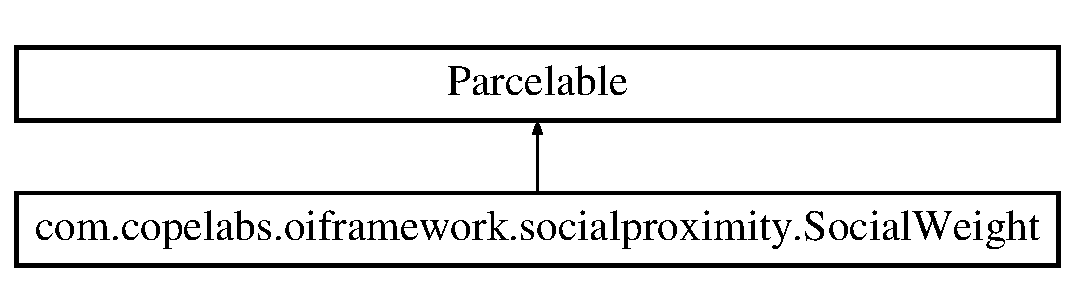
\includegraphics[height=2.000000cm]{classcom_1_1copelabs_1_1oiframework_1_1socialproximity_1_1_social_weight}
\end{center}
\end{figure}
\subsection*{Public Member Functions}
\begin{DoxyCompactItemize}
\item 
\hyperlink{classcom_1_1copelabs_1_1oiframework_1_1socialproximity_1_1_social_weight_adb73b95da859d4f5141ad6e193a3a12a}{Social\+Weight} (String \hyperlink{classcom_1_1copelabs_1_1oiframework_1_1socialproximity_1_1_social_weight_a93b91c868be4a9d3e395d46242ab96c4}{m\+Mac\+Address}, String \hyperlink{classcom_1_1copelabs_1_1oiframework_1_1socialproximity_1_1_social_weight_a6fa473ff39400696fd831ca519170610}{m\+Device\+Name}, double \hyperlink{classcom_1_1copelabs_1_1oiframework_1_1socialproximity_1_1_social_weight_a4c005dbeda3565c7049babdb95a391c7}{m\+Social\+Weight})
\item 
void \hyperlink{classcom_1_1copelabs_1_1oiframework_1_1socialproximity_1_1_social_weight_ab219dfa486cb5220a3904869a4d485d1}{set\+Mac\+Address} (String \hyperlink{classcom_1_1copelabs_1_1oiframework_1_1socialproximity_1_1_social_weight_a93b91c868be4a9d3e395d46242ab96c4}{m\+Mac\+Address})
\item 
String \hyperlink{classcom_1_1copelabs_1_1oiframework_1_1socialproximity_1_1_social_weight_ae53f2525ef0342baf9caabf0dbd55002}{get\+Mac\+Address} ()
\item 
void \hyperlink{classcom_1_1copelabs_1_1oiframework_1_1socialproximity_1_1_social_weight_aa56d5e6bbbb7a4a4676ca0ff89aea0e7}{set\+Device\+Name} (String \hyperlink{classcom_1_1copelabs_1_1oiframework_1_1socialproximity_1_1_social_weight_a6fa473ff39400696fd831ca519170610}{m\+Device\+Name})
\item 
String \hyperlink{classcom_1_1copelabs_1_1oiframework_1_1socialproximity_1_1_social_weight_a6f29943fc1123265d1ec1db3ceedd432}{get\+Device\+Name} ()
\item 
void \hyperlink{classcom_1_1copelabs_1_1oiframework_1_1socialproximity_1_1_social_weight_aa5fa343807ff1f465f49c60afe44808b}{set\+Social\+Weight} (long \hyperlink{classcom_1_1copelabs_1_1oiframework_1_1socialproximity_1_1_social_weight_a4c005dbeda3565c7049babdb95a391c7}{m\+Social\+Weight})
\item 
double \hyperlink{classcom_1_1copelabs_1_1oiframework_1_1socialproximity_1_1_social_weight_a3c360d68d35c9c141c1c8ba607a3b75a}{get\+Social\+Weight} ()
\item 
int \hyperlink{classcom_1_1copelabs_1_1oiframework_1_1socialproximity_1_1_social_weight_aca75f57e8d095eb7983ea4763c7f1f84}{describe\+Contents} ()
\item 
void \hyperlink{classcom_1_1copelabs_1_1oiframework_1_1socialproximity_1_1_social_weight_a043b33d2870a86e0b5917caee1998011}{write\+To\+Parcel} (Parcel dest, int flags)
\end{DoxyCompactItemize}
\subsection*{Public Attributes}
\begin{DoxyCompactItemize}
\item 
final Creator \hyperlink{classcom_1_1copelabs_1_1oiframework_1_1socialproximity_1_1_social_weight_a6bcb16eb1fe0d7db7cc1ca394b863efd}{C\+R\+E\+A\+T\+O\+R}
\end{DoxyCompactItemize}
\subsection*{Static Public Attributes}
\begin{DoxyCompactItemize}
\item 
static final String \hyperlink{classcom_1_1copelabs_1_1oiframework_1_1socialproximity_1_1_social_weight_a7f08f601ecd8ad6f108323f0d5a5d2b1}{social\+Weight\+\_\+key} = \char`\"{}social\+Receiver\char`\"{}
\end{DoxyCompactItemize}
\subsection*{Private Member Functions}
\begin{DoxyCompactItemize}
\item 
\hyperlink{classcom_1_1copelabs_1_1oiframework_1_1socialproximity_1_1_social_weight_a8171e0fc44f59be1a58ed7ef9be58362}{Social\+Weight} (Parcel source)
\end{DoxyCompactItemize}
\subsection*{Private Attributes}
\begin{DoxyCompactItemize}
\item 
String \hyperlink{classcom_1_1copelabs_1_1oiframework_1_1socialproximity_1_1_social_weight_a93b91c868be4a9d3e395d46242ab96c4}{m\+Mac\+Address}
\item 
String \hyperlink{classcom_1_1copelabs_1_1oiframework_1_1socialproximity_1_1_social_weight_a6fa473ff39400696fd831ca519170610}{m\+Device\+Name}
\item 
double \hyperlink{classcom_1_1copelabs_1_1oiframework_1_1socialproximity_1_1_social_weight_a4c005dbeda3565c7049babdb95a391c7}{m\+Social\+Weight}
\end{DoxyCompactItemize}


\subsection{Detailed Description}
\begin{DoxyVersion}{Version}
1.\+0 C\+O\+P\+Y\+R\+I\+G\+H\+T\+S C\+O\+P\+E\+L\+A\+B\+S/\+U\+L\+H\+T, L\+G\+P\+Lv3.\+0, 06-\/04-\/2016 This class holds information about a device\+: name, M\+A\+C address, and social weight towards it. 
\end{DoxyVersion}
\begin{DoxyAuthor}{Author}
Waldir Moreira (C\+O\+P\+E\+L\+A\+B\+S/\+U\+L\+H\+T) 
\end{DoxyAuthor}


\subsection{Constructor \& Destructor Documentation}
\hypertarget{classcom_1_1copelabs_1_1oiframework_1_1socialproximity_1_1_social_weight_adb73b95da859d4f5141ad6e193a3a12a}{}\index{com\+::copelabs\+::oiframework\+::socialproximity\+::\+Social\+Weight@{com\+::copelabs\+::oiframework\+::socialproximity\+::\+Social\+Weight}!Social\+Weight@{Social\+Weight}}
\index{Social\+Weight@{Social\+Weight}!com\+::copelabs\+::oiframework\+::socialproximity\+::\+Social\+Weight@{com\+::copelabs\+::oiframework\+::socialproximity\+::\+Social\+Weight}}
\subsubsection[{Social\+Weight(\+String m\+Mac\+Address, String m\+Device\+Name, double m\+Social\+Weight)}]{\setlength{\rightskip}{0pt plus 5cm}com.\+copelabs.\+oiframework.\+socialproximity.\+Social\+Weight.\+Social\+Weight (
\begin{DoxyParamCaption}
\item[{String}]{m\+Mac\+Address, }
\item[{String}]{m\+Device\+Name, }
\item[{double}]{m\+Social\+Weight}
\end{DoxyParamCaption}
)}\label{classcom_1_1copelabs_1_1oiframework_1_1socialproximity_1_1_social_weight_adb73b95da859d4f5141ad6e193a3a12a}
This method is the constructor for \hyperlink{classcom_1_1copelabs_1_1oiframework_1_1socialproximity_1_1_social_weight}{Social\+Weight}. 
\begin{DoxyParams}{Parameters}
{\em m\+Mac\+Address} & The M\+A\+C address of the device. \\
\hline
{\em m\+Device\+Name} & The name of the device. \\
\hline
{\em m\+Social\+Weight} & The social weight towards the device. \\
\hline
\end{DoxyParams}
\hypertarget{classcom_1_1copelabs_1_1oiframework_1_1socialproximity_1_1_social_weight_a8171e0fc44f59be1a58ed7ef9be58362}{}\index{com\+::copelabs\+::oiframework\+::socialproximity\+::\+Social\+Weight@{com\+::copelabs\+::oiframework\+::socialproximity\+::\+Social\+Weight}!Social\+Weight@{Social\+Weight}}
\index{Social\+Weight@{Social\+Weight}!com\+::copelabs\+::oiframework\+::socialproximity\+::\+Social\+Weight@{com\+::copelabs\+::oiframework\+::socialproximity\+::\+Social\+Weight}}
\subsubsection[{Social\+Weight(\+Parcel source)}]{\setlength{\rightskip}{0pt plus 5cm}com.\+copelabs.\+oiframework.\+socialproximity.\+Social\+Weight.\+Social\+Weight (
\begin{DoxyParamCaption}
\item[{Parcel}]{source}
\end{DoxyParamCaption}
)\hspace{0.3cm}{\ttfamily [private]}}\label{classcom_1_1copelabs_1_1oiframework_1_1socialproximity_1_1_social_weight_a8171e0fc44f59be1a58ed7ef9be58362}
This method is the constructor for \hyperlink{classcom_1_1copelabs_1_1oiframework_1_1socialproximity_1_1_social_weight}{Social\+Weight}. 
\begin{DoxyParams}{Parameters}
{\em source} & The Parcel source from which information can be extracted. \\
\hline
\end{DoxyParams}


\subsection{Member Function Documentation}
\hypertarget{classcom_1_1copelabs_1_1oiframework_1_1socialproximity_1_1_social_weight_aca75f57e8d095eb7983ea4763c7f1f84}{}\index{com\+::copelabs\+::oiframework\+::socialproximity\+::\+Social\+Weight@{com\+::copelabs\+::oiframework\+::socialproximity\+::\+Social\+Weight}!describe\+Contents@{describe\+Contents}}
\index{describe\+Contents@{describe\+Contents}!com\+::copelabs\+::oiframework\+::socialproximity\+::\+Social\+Weight@{com\+::copelabs\+::oiframework\+::socialproximity\+::\+Social\+Weight}}
\subsubsection[{describe\+Contents()}]{\setlength{\rightskip}{0pt plus 5cm}int com.\+copelabs.\+oiframework.\+socialproximity.\+Social\+Weight.\+describe\+Contents (
\begin{DoxyParamCaption}
{}
\end{DoxyParamCaption}
)}\label{classcom_1_1copelabs_1_1oiframework_1_1socialproximity_1_1_social_weight_aca75f57e8d095eb7983ea4763c7f1f84}
\hypertarget{classcom_1_1copelabs_1_1oiframework_1_1socialproximity_1_1_social_weight_a6f29943fc1123265d1ec1db3ceedd432}{}\index{com\+::copelabs\+::oiframework\+::socialproximity\+::\+Social\+Weight@{com\+::copelabs\+::oiframework\+::socialproximity\+::\+Social\+Weight}!get\+Device\+Name@{get\+Device\+Name}}
\index{get\+Device\+Name@{get\+Device\+Name}!com\+::copelabs\+::oiframework\+::socialproximity\+::\+Social\+Weight@{com\+::copelabs\+::oiframework\+::socialproximity\+::\+Social\+Weight}}
\subsubsection[{get\+Device\+Name()}]{\setlength{\rightskip}{0pt plus 5cm}String com.\+copelabs.\+oiframework.\+socialproximity.\+Social\+Weight.\+get\+Device\+Name (
\begin{DoxyParamCaption}
{}
\end{DoxyParamCaption}
)}\label{classcom_1_1copelabs_1_1oiframework_1_1socialproximity_1_1_social_weight_a6f29943fc1123265d1ec1db3ceedd432}
This method gets the device\textquotesingle{}s name. \hypertarget{classcom_1_1copelabs_1_1oiframework_1_1socialproximity_1_1_social_weight_ae53f2525ef0342baf9caabf0dbd55002}{}\index{com\+::copelabs\+::oiframework\+::socialproximity\+::\+Social\+Weight@{com\+::copelabs\+::oiframework\+::socialproximity\+::\+Social\+Weight}!get\+Mac\+Address@{get\+Mac\+Address}}
\index{get\+Mac\+Address@{get\+Mac\+Address}!com\+::copelabs\+::oiframework\+::socialproximity\+::\+Social\+Weight@{com\+::copelabs\+::oiframework\+::socialproximity\+::\+Social\+Weight}}
\subsubsection[{get\+Mac\+Address()}]{\setlength{\rightskip}{0pt plus 5cm}String com.\+copelabs.\+oiframework.\+socialproximity.\+Social\+Weight.\+get\+Mac\+Address (
\begin{DoxyParamCaption}
{}
\end{DoxyParamCaption}
)}\label{classcom_1_1copelabs_1_1oiframework_1_1socialproximity_1_1_social_weight_ae53f2525ef0342baf9caabf0dbd55002}
This method gets the device\textquotesingle{}s M\+A\+C address. \hypertarget{classcom_1_1copelabs_1_1oiframework_1_1socialproximity_1_1_social_weight_a3c360d68d35c9c141c1c8ba607a3b75a}{}\index{com\+::copelabs\+::oiframework\+::socialproximity\+::\+Social\+Weight@{com\+::copelabs\+::oiframework\+::socialproximity\+::\+Social\+Weight}!get\+Social\+Weight@{get\+Social\+Weight}}
\index{get\+Social\+Weight@{get\+Social\+Weight}!com\+::copelabs\+::oiframework\+::socialproximity\+::\+Social\+Weight@{com\+::copelabs\+::oiframework\+::socialproximity\+::\+Social\+Weight}}
\subsubsection[{get\+Social\+Weight()}]{\setlength{\rightskip}{0pt plus 5cm}double com.\+copelabs.\+oiframework.\+socialproximity.\+Social\+Weight.\+get\+Social\+Weight (
\begin{DoxyParamCaption}
{}
\end{DoxyParamCaption}
)}\label{classcom_1_1copelabs_1_1oiframework_1_1socialproximity_1_1_social_weight_a3c360d68d35c9c141c1c8ba607a3b75a}
This method gets the device\textquotesingle{}s social weight. \hypertarget{classcom_1_1copelabs_1_1oiframework_1_1socialproximity_1_1_social_weight_aa56d5e6bbbb7a4a4676ca0ff89aea0e7}{}\index{com\+::copelabs\+::oiframework\+::socialproximity\+::\+Social\+Weight@{com\+::copelabs\+::oiframework\+::socialproximity\+::\+Social\+Weight}!set\+Device\+Name@{set\+Device\+Name}}
\index{set\+Device\+Name@{set\+Device\+Name}!com\+::copelabs\+::oiframework\+::socialproximity\+::\+Social\+Weight@{com\+::copelabs\+::oiframework\+::socialproximity\+::\+Social\+Weight}}
\subsubsection[{set\+Device\+Name(\+String m\+Device\+Name)}]{\setlength{\rightskip}{0pt plus 5cm}void com.\+copelabs.\+oiframework.\+socialproximity.\+Social\+Weight.\+set\+Device\+Name (
\begin{DoxyParamCaption}
\item[{String}]{m\+Device\+Name}
\end{DoxyParamCaption}
)}\label{classcom_1_1copelabs_1_1oiframework_1_1socialproximity_1_1_social_weight_aa56d5e6bbbb7a4a4676ca0ff89aea0e7}
This method sets the device\textquotesingle{}s name. 
\begin{DoxyParams}{Parameters}
{\em m\+Device\+Name} & The device\textquotesingle{}s name. \\
\hline
\end{DoxyParams}
\hypertarget{classcom_1_1copelabs_1_1oiframework_1_1socialproximity_1_1_social_weight_ab219dfa486cb5220a3904869a4d485d1}{}\index{com\+::copelabs\+::oiframework\+::socialproximity\+::\+Social\+Weight@{com\+::copelabs\+::oiframework\+::socialproximity\+::\+Social\+Weight}!set\+Mac\+Address@{set\+Mac\+Address}}
\index{set\+Mac\+Address@{set\+Mac\+Address}!com\+::copelabs\+::oiframework\+::socialproximity\+::\+Social\+Weight@{com\+::copelabs\+::oiframework\+::socialproximity\+::\+Social\+Weight}}
\subsubsection[{set\+Mac\+Address(\+String m\+Mac\+Address)}]{\setlength{\rightskip}{0pt plus 5cm}void com.\+copelabs.\+oiframework.\+socialproximity.\+Social\+Weight.\+set\+Mac\+Address (
\begin{DoxyParamCaption}
\item[{String}]{m\+Mac\+Address}
\end{DoxyParamCaption}
)}\label{classcom_1_1copelabs_1_1oiframework_1_1socialproximity_1_1_social_weight_ab219dfa486cb5220a3904869a4d485d1}
This method sets the device\textquotesingle{}s M\+A\+C address. 
\begin{DoxyParams}{Parameters}
{\em m\+Mac\+Address} & The device\textquotesingle{}s M\+A\+C address. \\
\hline
\end{DoxyParams}
\hypertarget{classcom_1_1copelabs_1_1oiframework_1_1socialproximity_1_1_social_weight_aa5fa343807ff1f465f49c60afe44808b}{}\index{com\+::copelabs\+::oiframework\+::socialproximity\+::\+Social\+Weight@{com\+::copelabs\+::oiframework\+::socialproximity\+::\+Social\+Weight}!set\+Social\+Weight@{set\+Social\+Weight}}
\index{set\+Social\+Weight@{set\+Social\+Weight}!com\+::copelabs\+::oiframework\+::socialproximity\+::\+Social\+Weight@{com\+::copelabs\+::oiframework\+::socialproximity\+::\+Social\+Weight}}
\subsubsection[{set\+Social\+Weight(long m\+Social\+Weight)}]{\setlength{\rightskip}{0pt plus 5cm}void com.\+copelabs.\+oiframework.\+socialproximity.\+Social\+Weight.\+set\+Social\+Weight (
\begin{DoxyParamCaption}
\item[{long}]{m\+Social\+Weight}
\end{DoxyParamCaption}
)}\label{classcom_1_1copelabs_1_1oiframework_1_1socialproximity_1_1_social_weight_aa5fa343807ff1f465f49c60afe44808b}
This method sets the device\textquotesingle{}s social weight. 
\begin{DoxyParams}{Parameters}
{\em m\+Social\+Weight} & The device\textquotesingle{}s social weight. \\
\hline
\end{DoxyParams}
\hypertarget{classcom_1_1copelabs_1_1oiframework_1_1socialproximity_1_1_social_weight_a043b33d2870a86e0b5917caee1998011}{}\index{com\+::copelabs\+::oiframework\+::socialproximity\+::\+Social\+Weight@{com\+::copelabs\+::oiframework\+::socialproximity\+::\+Social\+Weight}!write\+To\+Parcel@{write\+To\+Parcel}}
\index{write\+To\+Parcel@{write\+To\+Parcel}!com\+::copelabs\+::oiframework\+::socialproximity\+::\+Social\+Weight@{com\+::copelabs\+::oiframework\+::socialproximity\+::\+Social\+Weight}}
\subsubsection[{write\+To\+Parcel(\+Parcel dest, int flags)}]{\setlength{\rightskip}{0pt plus 5cm}void com.\+copelabs.\+oiframework.\+socialproximity.\+Social\+Weight.\+write\+To\+Parcel (
\begin{DoxyParamCaption}
\item[{Parcel}]{dest, }
\item[{int}]{flags}
\end{DoxyParamCaption}
)}\label{classcom_1_1copelabs_1_1oiframework_1_1socialproximity_1_1_social_weight_a043b33d2870a86e0b5917caee1998011}


\subsection{Member Data Documentation}
\hypertarget{classcom_1_1copelabs_1_1oiframework_1_1socialproximity_1_1_social_weight_a6bcb16eb1fe0d7db7cc1ca394b863efd}{}\index{com\+::copelabs\+::oiframework\+::socialproximity\+::\+Social\+Weight@{com\+::copelabs\+::oiframework\+::socialproximity\+::\+Social\+Weight}!C\+R\+E\+A\+T\+O\+R@{C\+R\+E\+A\+T\+O\+R}}
\index{C\+R\+E\+A\+T\+O\+R@{C\+R\+E\+A\+T\+O\+R}!com\+::copelabs\+::oiframework\+::socialproximity\+::\+Social\+Weight@{com\+::copelabs\+::oiframework\+::socialproximity\+::\+Social\+Weight}}
\subsubsection[{C\+R\+E\+A\+T\+O\+R}]{\setlength{\rightskip}{0pt plus 5cm}final Creator com.\+copelabs.\+oiframework.\+socialproximity.\+Social\+Weight.\+C\+R\+E\+A\+T\+O\+R}\label{classcom_1_1copelabs_1_1oiframework_1_1socialproximity_1_1_social_weight_a6bcb16eb1fe0d7db7cc1ca394b863efd}
{\bfseries Initial value\+:}
\begin{DoxyCode}
= \textcolor{keyword}{new} Creator() \{
        @Override
        \textcolor{keyword}{public} \hyperlink{classcom_1_1copelabs_1_1oiframework_1_1socialproximity_1_1_social_weight_adb73b95da859d4f5141ad6e193a3a12a}{SocialWeight} createFromParcel(Parcel in) \{
            \textcolor{keywordflow}{return} \textcolor{keyword}{new} \hyperlink{classcom_1_1copelabs_1_1oiframework_1_1socialproximity_1_1_social_weight_adb73b95da859d4f5141ad6e193a3a12a}{SocialWeight}(in);
        \}
        @Override
        \textcolor{keyword}{public} \hyperlink{classcom_1_1copelabs_1_1oiframework_1_1socialproximity_1_1_social_weight_adb73b95da859d4f5141ad6e193a3a12a}{SocialWeight}[] newArray(\textcolor{keywordtype}{int} size) \{
            \textcolor{keywordflow}{return} \textcolor{keyword}{new} \hyperlink{classcom_1_1copelabs_1_1oiframework_1_1socialproximity_1_1_social_weight_adb73b95da859d4f5141ad6e193a3a12a}{SocialWeight}[size];
        \}
    \}
\end{DoxyCode}
\hypertarget{classcom_1_1copelabs_1_1oiframework_1_1socialproximity_1_1_social_weight_a6fa473ff39400696fd831ca519170610}{}\index{com\+::copelabs\+::oiframework\+::socialproximity\+::\+Social\+Weight@{com\+::copelabs\+::oiframework\+::socialproximity\+::\+Social\+Weight}!m\+Device\+Name@{m\+Device\+Name}}
\index{m\+Device\+Name@{m\+Device\+Name}!com\+::copelabs\+::oiframework\+::socialproximity\+::\+Social\+Weight@{com\+::copelabs\+::oiframework\+::socialproximity\+::\+Social\+Weight}}
\subsubsection[{m\+Device\+Name}]{\setlength{\rightskip}{0pt plus 5cm}String com.\+copelabs.\+oiframework.\+socialproximity.\+Social\+Weight.\+m\+Device\+Name\hspace{0.3cm}{\ttfamily [private]}}\label{classcom_1_1copelabs_1_1oiframework_1_1socialproximity_1_1_social_weight_a6fa473ff39400696fd831ca519170610}
\hypertarget{classcom_1_1copelabs_1_1oiframework_1_1socialproximity_1_1_social_weight_a93b91c868be4a9d3e395d46242ab96c4}{}\index{com\+::copelabs\+::oiframework\+::socialproximity\+::\+Social\+Weight@{com\+::copelabs\+::oiframework\+::socialproximity\+::\+Social\+Weight}!m\+Mac\+Address@{m\+Mac\+Address}}
\index{m\+Mac\+Address@{m\+Mac\+Address}!com\+::copelabs\+::oiframework\+::socialproximity\+::\+Social\+Weight@{com\+::copelabs\+::oiframework\+::socialproximity\+::\+Social\+Weight}}
\subsubsection[{m\+Mac\+Address}]{\setlength{\rightskip}{0pt plus 5cm}String com.\+copelabs.\+oiframework.\+socialproximity.\+Social\+Weight.\+m\+Mac\+Address\hspace{0.3cm}{\ttfamily [private]}}\label{classcom_1_1copelabs_1_1oiframework_1_1socialproximity_1_1_social_weight_a93b91c868be4a9d3e395d46242ab96c4}
\hypertarget{classcom_1_1copelabs_1_1oiframework_1_1socialproximity_1_1_social_weight_a4c005dbeda3565c7049babdb95a391c7}{}\index{com\+::copelabs\+::oiframework\+::socialproximity\+::\+Social\+Weight@{com\+::copelabs\+::oiframework\+::socialproximity\+::\+Social\+Weight}!m\+Social\+Weight@{m\+Social\+Weight}}
\index{m\+Social\+Weight@{m\+Social\+Weight}!com\+::copelabs\+::oiframework\+::socialproximity\+::\+Social\+Weight@{com\+::copelabs\+::oiframework\+::socialproximity\+::\+Social\+Weight}}
\subsubsection[{m\+Social\+Weight}]{\setlength{\rightskip}{0pt plus 5cm}double com.\+copelabs.\+oiframework.\+socialproximity.\+Social\+Weight.\+m\+Social\+Weight\hspace{0.3cm}{\ttfamily [private]}}\label{classcom_1_1copelabs_1_1oiframework_1_1socialproximity_1_1_social_weight_a4c005dbeda3565c7049babdb95a391c7}
\hypertarget{classcom_1_1copelabs_1_1oiframework_1_1socialproximity_1_1_social_weight_a7f08f601ecd8ad6f108323f0d5a5d2b1}{}\index{com\+::copelabs\+::oiframework\+::socialproximity\+::\+Social\+Weight@{com\+::copelabs\+::oiframework\+::socialproximity\+::\+Social\+Weight}!social\+Weight\+\_\+key@{social\+Weight\+\_\+key}}
\index{social\+Weight\+\_\+key@{social\+Weight\+\_\+key}!com\+::copelabs\+::oiframework\+::socialproximity\+::\+Social\+Weight@{com\+::copelabs\+::oiframework\+::socialproximity\+::\+Social\+Weight}}
\subsubsection[{social\+Weight\+\_\+key}]{\setlength{\rightskip}{0pt plus 5cm}final String com.\+copelabs.\+oiframework.\+socialproximity.\+Social\+Weight.\+social\+Weight\+\_\+key = \char`\"{}social\+Receiver\char`\"{}\hspace{0.3cm}{\ttfamily [static]}}\label{classcom_1_1copelabs_1_1oiframework_1_1socialproximity_1_1_social_weight_a7f08f601ecd8ad6f108323f0d5a5d2b1}


The documentation for this class was generated from the following file\+:\begin{DoxyCompactItemize}
\item 
src/com/copelabs/oiframework/socialproximity/\hyperlink{_social_weight_8java}{Social\+Weight.\+java}\end{DoxyCompactItemize}

\hypertarget{classcom_1_1copelabs_1_1oiframework_1_1socialproximity_1_1_s_q_lite_helper}{}\section{com.\+copelabs.\+oiframework.\+socialproximity.\+S\+Q\+Lite\+Helper Class Reference}
\label{classcom_1_1copelabs_1_1oiframework_1_1socialproximity_1_1_s_q_lite_helper}\index{com.\+copelabs.\+oiframework.\+socialproximity.\+S\+Q\+Lite\+Helper@{com.\+copelabs.\+oiframework.\+socialproximity.\+S\+Q\+Lite\+Helper}}
Inheritance diagram for com.\+copelabs.\+oiframework.\+socialproximity.\+S\+Q\+Lite\+Helper\+:\begin{figure}[H]
\begin{center}
\leavevmode
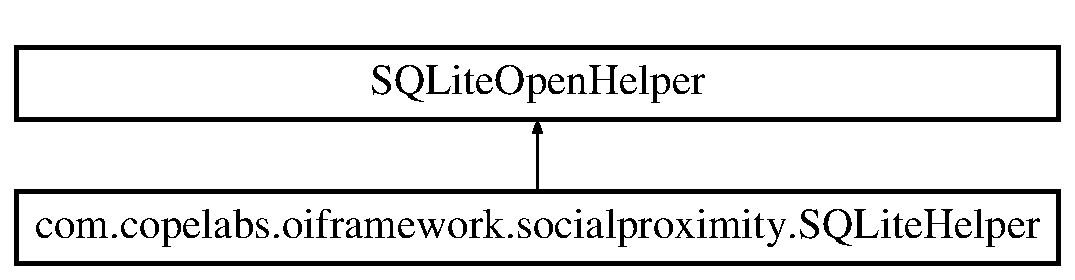
\includegraphics[height=2.000000cm]{classcom_1_1copelabs_1_1oiframework_1_1socialproximity_1_1_s_q_lite_helper}
\end{center}
\end{figure}
\subsection*{Public Member Functions}
\begin{DoxyCompactItemize}
\item 
\hyperlink{classcom_1_1copelabs_1_1oiframework_1_1socialproximity_1_1_s_q_lite_helper_a5d8b03643c0e686cc8450eca42114091}{S\+Q\+Lite\+Helper} (Context context)
\item 
void \hyperlink{classcom_1_1copelabs_1_1oiframework_1_1socialproximity_1_1_s_q_lite_helper_a6352e58e02fcfc927bf783e2e5b6d405}{on\+Create} (S\+Q\+Lite\+Database data\+Base)
\item 
void \hyperlink{classcom_1_1copelabs_1_1oiframework_1_1socialproximity_1_1_s_q_lite_helper_af98ddb015b61218a9cfe64c5e76b8868}{on\+Upgrade} (S\+Q\+Lite\+Database data\+Base, int old\+Version, int new\+Version)
\end{DoxyCompactItemize}
\subsection*{Static Public Attributes}
\begin{DoxyCompactItemize}
\item 
static final String \hyperlink{classcom_1_1copelabs_1_1oiframework_1_1socialproximity_1_1_s_q_lite_helper_a1c11ba652a7d7221c90f773c4edb2af3}{T\+A\+B\+L\+E\+\_\+\+B\+T\+D\+E\+V\+I\+C\+E} = \char`\"{}btdevices\char`\"{}
\item 
static final String \hyperlink{classcom_1_1copelabs_1_1oiframework_1_1socialproximity_1_1_s_q_lite_helper_ab31b56a0eac0e440f57ad05a777f42be}{T\+A\+B\+L\+E\+\_\+\+B\+T\+D\+E\+V\+I\+C\+E\+E\+N\+C\+O\+U\+N\+T\+E\+R\+D\+U\+R\+A\+T\+I\+O\+N} = \char`\"{}btdevice\+\_\+encounterduration\char`\"{}
\item 
static final String \hyperlink{classcom_1_1copelabs_1_1oiframework_1_1socialproximity_1_1_s_q_lite_helper_acfb9d1512f69c1299ca39bf979ae7911}{T\+A\+B\+L\+E\+\_\+\+B\+T\+D\+E\+V\+I\+C\+E\+A\+V\+E\+R\+A\+G\+E\+E\+N\+C\+O\+U\+N\+T\+E\+R\+D\+U\+R\+A\+T\+I\+O\+N} = \char`\"{}btdevice\+\_\+averageencounterduration\char`\"{}
\item 
static final String \hyperlink{classcom_1_1copelabs_1_1oiframework_1_1socialproximity_1_1_s_q_lite_helper_ad91da6d89af9550e074a14a62f3366b1}{T\+A\+B\+L\+E\+\_\+\+B\+T\+D\+E\+V\+I\+C\+E\+S\+O\+C\+I\+A\+L\+W\+E\+I\+G\+H\+T} = \char`\"{}btdevice\+\_\+socialweight\char`\"{}
\item 
static final String \hyperlink{classcom_1_1copelabs_1_1oiframework_1_1socialproximity_1_1_s_q_lite_helper_a42da605a2e3ade18adf5dd701eb48b06}{C\+O\+L\+U\+M\+N\+\_\+\+I\+D} = \char`\"{}\+\_\+id\char`\"{}
\item 
static final String \hyperlink{classcom_1_1copelabs_1_1oiframework_1_1socialproximity_1_1_s_q_lite_helper_aa664c2d0219f93cc556b30e4b48954c1}{C\+O\+L\+U\+M\+N\+\_\+\+B\+T\+D\+E\+V\+\_\+\+M\+A\+C\+\_\+\+A\+D\+D\+R\+E\+S\+S} = \char`\"{}dev\+Bt\+Mac\+Add\char`\"{}
\item 
static final String \hyperlink{classcom_1_1copelabs_1_1oiframework_1_1socialproximity_1_1_s_q_lite_helper_adedd7238a8b391cf633df141dbc1f913}{C\+O\+L\+U\+M\+N\+\_\+\+B\+T\+D\+E\+V\+\_\+\+N\+A\+M\+E} = \char`\"{}dev\+Name\char`\"{}
\item 
static final String \hyperlink{classcom_1_1copelabs_1_1oiframework_1_1socialproximity_1_1_s_q_lite_helper_a8e8c6e04e4faa05d62f318698f021cbe}{C\+O\+L\+U\+M\+N\+\_\+\+B\+T\+D\+E\+V\+\_\+\+E\+N\+C\+O\+U\+N\+T\+E\+R\+S\+T\+A\+R\+T} = \char`\"{}dev\+Encounter\+Start\char`\"{}
\item 
static final String \hyperlink{classcom_1_1copelabs_1_1oiframework_1_1socialproximity_1_1_s_q_lite_helper_a4ef08ec127537c8cd3945d05ef9ebb5b}{C\+O\+L\+U\+M\+N\+\_\+\+B\+T\+D\+E\+V\+\_\+\+E\+N\+C\+O\+U\+N\+T\+E\+R\+D\+U\+R\+A\+T\+I\+O\+N\+\_\+\+S\+L\+O\+T1} = \char`\"{}dev\+Encounter\+Duration\+\_\+slot1\char`\"{}
\item 
static final String \hyperlink{classcom_1_1copelabs_1_1oiframework_1_1socialproximity_1_1_s_q_lite_helper_a13ed1ee3d7a8645bbd511ccb9fa1e8e1}{C\+O\+L\+U\+M\+N\+\_\+\+B\+T\+D\+E\+V\+\_\+\+E\+N\+C\+O\+U\+N\+T\+E\+R\+D\+U\+R\+A\+T\+I\+O\+N\+\_\+\+S\+L\+O\+T2} = \char`\"{}dev\+Encounter\+Duration\+\_\+slot2\char`\"{}
\item 
static final String \hyperlink{classcom_1_1copelabs_1_1oiframework_1_1socialproximity_1_1_s_q_lite_helper_a1581408605a4e12d35dd1e3977ac74a8}{C\+O\+L\+U\+M\+N\+\_\+\+B\+T\+D\+E\+V\+\_\+\+E\+N\+C\+O\+U\+N\+T\+E\+R\+D\+U\+R\+A\+T\+I\+O\+N\+\_\+\+S\+L\+O\+T3} = \char`\"{}dev\+Encounter\+Duration\+\_\+slot3\char`\"{}
\item 
static final String \hyperlink{classcom_1_1copelabs_1_1oiframework_1_1socialproximity_1_1_s_q_lite_helper_a57d2e17fbe8da0029e9c2aec589ac2a9}{C\+O\+L\+U\+M\+N\+\_\+\+B\+T\+D\+E\+V\+\_\+\+E\+N\+C\+O\+U\+N\+T\+E\+R\+D\+U\+R\+A\+T\+I\+O\+N\+\_\+\+S\+L\+O\+T4} = \char`\"{}dev\+Encounter\+Duration\+\_\+slot4\char`\"{}
\item 
static final String \hyperlink{classcom_1_1copelabs_1_1oiframework_1_1socialproximity_1_1_s_q_lite_helper_a0ec9e7d9918140c8438c33b336cf096a}{C\+O\+L\+U\+M\+N\+\_\+\+B\+T\+D\+E\+V\+\_\+\+E\+N\+C\+O\+U\+N\+T\+E\+R\+D\+U\+R\+A\+T\+I\+O\+N\+\_\+\+S\+L\+O\+T5} = \char`\"{}dev\+Encounter\+Duration\+\_\+slot5\char`\"{}
\item 
static final String \hyperlink{classcom_1_1copelabs_1_1oiframework_1_1socialproximity_1_1_s_q_lite_helper_a28b277aecd4b5af8c05909bc3228db5f}{C\+O\+L\+U\+M\+N\+\_\+\+B\+T\+D\+E\+V\+\_\+\+E\+N\+C\+O\+U\+N\+T\+E\+R\+D\+U\+R\+A\+T\+I\+O\+N\+\_\+\+S\+L\+O\+T6} = \char`\"{}dev\+Encounter\+Duration\+\_\+slot6\char`\"{}
\item 
static final String \hyperlink{classcom_1_1copelabs_1_1oiframework_1_1socialproximity_1_1_s_q_lite_helper_ac9d86b61d1797abeaf26b2a79b46953d}{C\+O\+L\+U\+M\+N\+\_\+\+B\+T\+D\+E\+V\+\_\+\+E\+N\+C\+O\+U\+N\+T\+E\+R\+D\+U\+R\+A\+T\+I\+O\+N\+\_\+\+S\+L\+O\+T7} = \char`\"{}dev\+Encounter\+Duration\+\_\+slot7\char`\"{}
\item 
static final String \hyperlink{classcom_1_1copelabs_1_1oiframework_1_1socialproximity_1_1_s_q_lite_helper_a3c3c339ebd629e17b3213ca2f68c4ebd}{C\+O\+L\+U\+M\+N\+\_\+\+B\+T\+D\+E\+V\+\_\+\+E\+N\+C\+O\+U\+N\+T\+E\+R\+D\+U\+R\+A\+T\+I\+O\+N\+\_\+\+S\+L\+O\+T8} = \char`\"{}dev\+Encounter\+Duration\+\_\+slot8\char`\"{}
\item 
static final String \hyperlink{classcom_1_1copelabs_1_1oiframework_1_1socialproximity_1_1_s_q_lite_helper_aa83e807bb41ffcbe2d4def924ab1e348}{C\+O\+L\+U\+M\+N\+\_\+\+B\+T\+D\+E\+V\+\_\+\+E\+N\+C\+O\+U\+N\+T\+E\+R\+D\+U\+R\+A\+T\+I\+O\+N\+\_\+\+S\+L\+O\+T9} = \char`\"{}dev\+Encounter\+Duration\+\_\+slot9\char`\"{}
\item 
static final String \hyperlink{classcom_1_1copelabs_1_1oiframework_1_1socialproximity_1_1_s_q_lite_helper_a44cdf46d6a1763bf54a61c202188312d}{C\+O\+L\+U\+M\+N\+\_\+\+B\+T\+D\+E\+V\+\_\+\+E\+N\+C\+O\+U\+N\+T\+E\+R\+D\+U\+R\+A\+T\+I\+O\+N\+\_\+\+S\+L\+O\+T10} = \char`\"{}dev\+Encounter\+Duration\+\_\+slot10\char`\"{}
\item 
static final String \hyperlink{classcom_1_1copelabs_1_1oiframework_1_1socialproximity_1_1_s_q_lite_helper_add0e848d049869ca8b058fd6f8465f63}{C\+O\+L\+U\+M\+N\+\_\+\+B\+T\+D\+E\+V\+\_\+\+E\+N\+C\+O\+U\+N\+T\+E\+R\+D\+U\+R\+A\+T\+I\+O\+N\+\_\+\+S\+L\+O\+T11} = \char`\"{}dev\+Encounter\+Duration\+\_\+slot11\char`\"{}
\item 
static final String \hyperlink{classcom_1_1copelabs_1_1oiframework_1_1socialproximity_1_1_s_q_lite_helper_a6fc6ec1c8e4a832378c2481ef7510642}{C\+O\+L\+U\+M\+N\+\_\+\+B\+T\+D\+E\+V\+\_\+\+E\+N\+C\+O\+U\+N\+T\+E\+R\+D\+U\+R\+A\+T\+I\+O\+N\+\_\+\+S\+L\+O\+T12} = \char`\"{}dev\+Encounter\+Duration\+\_\+slot12\char`\"{}
\item 
static final String \hyperlink{classcom_1_1copelabs_1_1oiframework_1_1socialproximity_1_1_s_q_lite_helper_ae870950e44e1f97bfb360d1619b75796}{C\+O\+L\+U\+M\+N\+\_\+\+B\+T\+D\+E\+V\+\_\+\+E\+N\+C\+O\+U\+N\+T\+E\+R\+D\+U\+R\+A\+T\+I\+O\+N\+\_\+\+S\+L\+O\+T13} = \char`\"{}dev\+Encounter\+Duration\+\_\+slot13\char`\"{}
\item 
static final String \hyperlink{classcom_1_1copelabs_1_1oiframework_1_1socialproximity_1_1_s_q_lite_helper_a4b653e54a4fe2c7a5b446abbed929aa3}{C\+O\+L\+U\+M\+N\+\_\+\+B\+T\+D\+E\+V\+\_\+\+E\+N\+C\+O\+U\+N\+T\+E\+R\+D\+U\+R\+A\+T\+I\+O\+N\+\_\+\+S\+L\+O\+T14} = \char`\"{}dev\+Encounter\+Duration\+\_\+slot14\char`\"{}
\item 
static final String \hyperlink{classcom_1_1copelabs_1_1oiframework_1_1socialproximity_1_1_s_q_lite_helper_af8916712e22421bfb27c17934dc19bf6}{C\+O\+L\+U\+M\+N\+\_\+\+B\+T\+D\+E\+V\+\_\+\+E\+N\+C\+O\+U\+N\+T\+E\+R\+D\+U\+R\+A\+T\+I\+O\+N\+\_\+\+S\+L\+O\+T15} = \char`\"{}dev\+Encounter\+Duration\+\_\+slot15\char`\"{}
\item 
static final String \hyperlink{classcom_1_1copelabs_1_1oiframework_1_1socialproximity_1_1_s_q_lite_helper_a4ef85302cf258bdda8ab288488a27614}{C\+O\+L\+U\+M\+N\+\_\+\+B\+T\+D\+E\+V\+\_\+\+E\+N\+C\+O\+U\+N\+T\+E\+R\+D\+U\+R\+A\+T\+I\+O\+N\+\_\+\+S\+L\+O\+T16} = \char`\"{}dev\+Encounter\+Duration\+\_\+slot16\char`\"{}
\item 
static final String \hyperlink{classcom_1_1copelabs_1_1oiframework_1_1socialproximity_1_1_s_q_lite_helper_abe4d2d079d8870535425368d8e2a562a}{C\+O\+L\+U\+M\+N\+\_\+\+B\+T\+D\+E\+V\+\_\+\+E\+N\+C\+O\+U\+N\+T\+E\+R\+D\+U\+R\+A\+T\+I\+O\+N\+\_\+\+S\+L\+O\+T17} = \char`\"{}dev\+Encounter\+Duration\+\_\+slot17\char`\"{}
\item 
static final String \hyperlink{classcom_1_1copelabs_1_1oiframework_1_1socialproximity_1_1_s_q_lite_helper_adc550089f462600d2fef7b81986fd217}{C\+O\+L\+U\+M\+N\+\_\+\+B\+T\+D\+E\+V\+\_\+\+E\+N\+C\+O\+U\+N\+T\+E\+R\+D\+U\+R\+A\+T\+I\+O\+N\+\_\+\+S\+L\+O\+T18} = \char`\"{}dev\+Encounter\+Duration\+\_\+slot18\char`\"{}
\item 
static final String \hyperlink{classcom_1_1copelabs_1_1oiframework_1_1socialproximity_1_1_s_q_lite_helper_af3fb4759e642965c9dc97713aedb9c7a}{C\+O\+L\+U\+M\+N\+\_\+\+B\+T\+D\+E\+V\+\_\+\+E\+N\+C\+O\+U\+N\+T\+E\+R\+D\+U\+R\+A\+T\+I\+O\+N\+\_\+\+S\+L\+O\+T19} = \char`\"{}dev\+Encounter\+Duration\+\_\+slot19\char`\"{}
\item 
static final String \hyperlink{classcom_1_1copelabs_1_1oiframework_1_1socialproximity_1_1_s_q_lite_helper_a79779a8ba3f8e445a4c9b3a9c242bab8}{C\+O\+L\+U\+M\+N\+\_\+\+B\+T\+D\+E\+V\+\_\+\+E\+N\+C\+O\+U\+N\+T\+E\+R\+D\+U\+R\+A\+T\+I\+O\+N\+\_\+\+S\+L\+O\+T20} = \char`\"{}dev\+Encounter\+Duration\+\_\+slot20\char`\"{}
\item 
static final String \hyperlink{classcom_1_1copelabs_1_1oiframework_1_1socialproximity_1_1_s_q_lite_helper_ab9f012c761286e358e37aceeb9354ff2}{C\+O\+L\+U\+M\+N\+\_\+\+B\+T\+D\+E\+V\+\_\+\+E\+N\+C\+O\+U\+N\+T\+E\+R\+D\+U\+R\+A\+T\+I\+O\+N\+\_\+\+S\+L\+O\+T21} = \char`\"{}dev\+Encounter\+Duration\+\_\+slot21\char`\"{}
\item 
static final String \hyperlink{classcom_1_1copelabs_1_1oiframework_1_1socialproximity_1_1_s_q_lite_helper_acb117913601710773e1abf9c34ef21e8}{C\+O\+L\+U\+M\+N\+\_\+\+B\+T\+D\+E\+V\+\_\+\+E\+N\+C\+O\+U\+N\+T\+E\+R\+D\+U\+R\+A\+T\+I\+O\+N\+\_\+\+S\+L\+O\+T22} = \char`\"{}dev\+Encounter\+Duration\+\_\+slot22\char`\"{}
\item 
static final String \hyperlink{classcom_1_1copelabs_1_1oiframework_1_1socialproximity_1_1_s_q_lite_helper_a20e3a923ddcf0df4318349a69851ec3b}{C\+O\+L\+U\+M\+N\+\_\+\+B\+T\+D\+E\+V\+\_\+\+E\+N\+C\+O\+U\+N\+T\+E\+R\+D\+U\+R\+A\+T\+I\+O\+N\+\_\+\+S\+L\+O\+T23} = \char`\"{}dev\+Encounter\+Duration\+\_\+slot23\char`\"{}
\item 
static final String \hyperlink{classcom_1_1copelabs_1_1oiframework_1_1socialproximity_1_1_s_q_lite_helper_a2c7cd6032d517eee9403df316b05f432}{C\+O\+L\+U\+M\+N\+\_\+\+B\+T\+D\+E\+V\+\_\+\+E\+N\+C\+O\+U\+N\+T\+E\+R\+D\+U\+R\+A\+T\+I\+O\+N\+\_\+\+S\+L\+O\+T24} = \char`\"{}dev\+Encounter\+Duration\+\_\+slot24\char`\"{}
\item 
static final String \hyperlink{classcom_1_1copelabs_1_1oiframework_1_1socialproximity_1_1_s_q_lite_helper_a1587f0eed87daf373cf8e595fa3061a0}{C\+O\+L\+U\+M\+N\+\_\+\+B\+T\+D\+E\+V\+\_\+\+A\+V\+G\+E\+N\+C\+O\+U\+N\+T\+E\+R\+D\+U\+R\+A\+T\+I\+O\+N\+\_\+\+S\+L\+O\+T1} = \char`\"{}dev\+Avg\+Encounter\+Duration\+\_\+slot1\char`\"{}
\item 
static final String \hyperlink{classcom_1_1copelabs_1_1oiframework_1_1socialproximity_1_1_s_q_lite_helper_aefeb1d706536288b9e0e606fe4ee6df1}{C\+O\+L\+U\+M\+N\+\_\+\+B\+T\+D\+E\+V\+\_\+\+A\+V\+G\+E\+N\+C\+O\+U\+N\+T\+E\+R\+D\+U\+R\+A\+T\+I\+O\+N\+\_\+\+S\+L\+O\+T2} = \char`\"{}dev\+Avg\+Encounter\+Duration\+\_\+slot2\char`\"{}
\item 
static final String \hyperlink{classcom_1_1copelabs_1_1oiframework_1_1socialproximity_1_1_s_q_lite_helper_a4f1f938f3722be2271d4593b1d8d3ac2}{C\+O\+L\+U\+M\+N\+\_\+\+B\+T\+D\+E\+V\+\_\+\+A\+V\+G\+E\+N\+C\+O\+U\+N\+T\+E\+R\+D\+U\+R\+A\+T\+I\+O\+N\+\_\+\+S\+L\+O\+T3} = \char`\"{}dev\+Avg\+Encounter\+Duration\+\_\+slot3\char`\"{}
\item 
static final String \hyperlink{classcom_1_1copelabs_1_1oiframework_1_1socialproximity_1_1_s_q_lite_helper_aa7f5e3c448045c6ea284cead8ada6280}{C\+O\+L\+U\+M\+N\+\_\+\+B\+T\+D\+E\+V\+\_\+\+A\+V\+G\+E\+N\+C\+O\+U\+N\+T\+E\+R\+D\+U\+R\+A\+T\+I\+O\+N\+\_\+\+S\+L\+O\+T4} = \char`\"{}dev\+Avg\+Encounter\+Duration\+\_\+slot4\char`\"{}
\item 
static final String \hyperlink{classcom_1_1copelabs_1_1oiframework_1_1socialproximity_1_1_s_q_lite_helper_a7d44e66e42425d636c452b9dbddec5db}{C\+O\+L\+U\+M\+N\+\_\+\+B\+T\+D\+E\+V\+\_\+\+A\+V\+G\+E\+N\+C\+O\+U\+N\+T\+E\+R\+D\+U\+R\+A\+T\+I\+O\+N\+\_\+\+S\+L\+O\+T5} = \char`\"{}dev\+Avg\+Encounter\+Duration\+\_\+slot5\char`\"{}
\item 
static final String \hyperlink{classcom_1_1copelabs_1_1oiframework_1_1socialproximity_1_1_s_q_lite_helper_a4c44d6f65c62d53bd276c79208d38348}{C\+O\+L\+U\+M\+N\+\_\+\+B\+T\+D\+E\+V\+\_\+\+A\+V\+G\+E\+N\+C\+O\+U\+N\+T\+E\+R\+D\+U\+R\+A\+T\+I\+O\+N\+\_\+\+S\+L\+O\+T6} = \char`\"{}dev\+Avg\+Encounter\+Duration\+\_\+slot6\char`\"{}
\item 
static final String \hyperlink{classcom_1_1copelabs_1_1oiframework_1_1socialproximity_1_1_s_q_lite_helper_ae6cfc9c5bc9e935cceaf7ca3e764b957}{C\+O\+L\+U\+M\+N\+\_\+\+B\+T\+D\+E\+V\+\_\+\+A\+V\+G\+E\+N\+C\+O\+U\+N\+T\+E\+R\+D\+U\+R\+A\+T\+I\+O\+N\+\_\+\+S\+L\+O\+T7} = \char`\"{}dev\+Avg\+Encounter\+Duration\+\_\+slot7\char`\"{}
\item 
static final String \hyperlink{classcom_1_1copelabs_1_1oiframework_1_1socialproximity_1_1_s_q_lite_helper_afa1acefb9ac52993d28799345bf94d49}{C\+O\+L\+U\+M\+N\+\_\+\+B\+T\+D\+E\+V\+\_\+\+A\+V\+G\+E\+N\+C\+O\+U\+N\+T\+E\+R\+D\+U\+R\+A\+T\+I\+O\+N\+\_\+\+S\+L\+O\+T8} = \char`\"{}dev\+Avg\+Encounter\+Duration\+\_\+slot8\char`\"{}
\item 
static final String \hyperlink{classcom_1_1copelabs_1_1oiframework_1_1socialproximity_1_1_s_q_lite_helper_a39c07bc84c3220997df50296c7d58ec0}{C\+O\+L\+U\+M\+N\+\_\+\+B\+T\+D\+E\+V\+\_\+\+A\+V\+G\+E\+N\+C\+O\+U\+N\+T\+E\+R\+D\+U\+R\+A\+T\+I\+O\+N\+\_\+\+S\+L\+O\+T9} = \char`\"{}dev\+Avg\+Encounter\+Duration\+\_\+slot9\char`\"{}
\item 
static final String \hyperlink{classcom_1_1copelabs_1_1oiframework_1_1socialproximity_1_1_s_q_lite_helper_ab21157b336ae9f13c90f0589426c9d81}{C\+O\+L\+U\+M\+N\+\_\+\+B\+T\+D\+E\+V\+\_\+\+A\+V\+G\+E\+N\+C\+O\+U\+N\+T\+E\+R\+D\+U\+R\+A\+T\+I\+O\+N\+\_\+\+S\+L\+O\+T10} = \char`\"{}dev\+Avg\+Encounter\+Duration\+\_\+slot10\char`\"{}
\item 
static final String \hyperlink{classcom_1_1copelabs_1_1oiframework_1_1socialproximity_1_1_s_q_lite_helper_aeb5a3e7fbf10b907bbe39cc8e693e486}{C\+O\+L\+U\+M\+N\+\_\+\+B\+T\+D\+E\+V\+\_\+\+A\+V\+G\+E\+N\+C\+O\+U\+N\+T\+E\+R\+D\+U\+R\+A\+T\+I\+O\+N\+\_\+\+S\+L\+O\+T11} = \char`\"{}dev\+Avg\+Encounter\+Duration\+\_\+slot11\char`\"{}
\item 
static final String \hyperlink{classcom_1_1copelabs_1_1oiframework_1_1socialproximity_1_1_s_q_lite_helper_abc1b287d4e4071776d025ff203f0cb70}{C\+O\+L\+U\+M\+N\+\_\+\+B\+T\+D\+E\+V\+\_\+\+A\+V\+G\+E\+N\+C\+O\+U\+N\+T\+E\+R\+D\+U\+R\+A\+T\+I\+O\+N\+\_\+\+S\+L\+O\+T12} = \char`\"{}dev\+Avg\+Encounter\+Duration\+\_\+slot12\char`\"{}
\item 
static final String \hyperlink{classcom_1_1copelabs_1_1oiframework_1_1socialproximity_1_1_s_q_lite_helper_a7e00e16a49501db8ef9d8345fb85444d}{C\+O\+L\+U\+M\+N\+\_\+\+B\+T\+D\+E\+V\+\_\+\+A\+V\+G\+E\+N\+C\+O\+U\+N\+T\+E\+R\+D\+U\+R\+A\+T\+I\+O\+N\+\_\+\+S\+L\+O\+T13} = \char`\"{}dev\+Avg\+Encounter\+Duration\+\_\+slot13\char`\"{}
\item 
static final String \hyperlink{classcom_1_1copelabs_1_1oiframework_1_1socialproximity_1_1_s_q_lite_helper_a9e0ee8840e3194657b740ea34d5ac3c2}{C\+O\+L\+U\+M\+N\+\_\+\+B\+T\+D\+E\+V\+\_\+\+A\+V\+G\+E\+N\+C\+O\+U\+N\+T\+E\+R\+D\+U\+R\+A\+T\+I\+O\+N\+\_\+\+S\+L\+O\+T14} = \char`\"{}dev\+Avg\+Encounter\+Duration\+\_\+slot14\char`\"{}
\item 
static final String \hyperlink{classcom_1_1copelabs_1_1oiframework_1_1socialproximity_1_1_s_q_lite_helper_a10ed1f74726e7c5904e0fb27b15867f9}{C\+O\+L\+U\+M\+N\+\_\+\+B\+T\+D\+E\+V\+\_\+\+A\+V\+G\+E\+N\+C\+O\+U\+N\+T\+E\+R\+D\+U\+R\+A\+T\+I\+O\+N\+\_\+\+S\+L\+O\+T15} = \char`\"{}dev\+Avg\+Encounter\+Duration\+\_\+slot15\char`\"{}
\item 
static final String \hyperlink{classcom_1_1copelabs_1_1oiframework_1_1socialproximity_1_1_s_q_lite_helper_ab893303f476ecb25a5dc9c5eef2124df}{C\+O\+L\+U\+M\+N\+\_\+\+B\+T\+D\+E\+V\+\_\+\+A\+V\+G\+E\+N\+C\+O\+U\+N\+T\+E\+R\+D\+U\+R\+A\+T\+I\+O\+N\+\_\+\+S\+L\+O\+T16} = \char`\"{}dev\+Avg\+Encounter\+Duration\+\_\+slot16\char`\"{}
\item 
static final String \hyperlink{classcom_1_1copelabs_1_1oiframework_1_1socialproximity_1_1_s_q_lite_helper_a98e049bd52b746d43944a63f42fff246}{C\+O\+L\+U\+M\+N\+\_\+\+B\+T\+D\+E\+V\+\_\+\+A\+V\+G\+E\+N\+C\+O\+U\+N\+T\+E\+R\+D\+U\+R\+A\+T\+I\+O\+N\+\_\+\+S\+L\+O\+T17} = \char`\"{}dev\+Avg\+Encounter\+Duration\+\_\+slot17\char`\"{}
\item 
static final String \hyperlink{classcom_1_1copelabs_1_1oiframework_1_1socialproximity_1_1_s_q_lite_helper_a509946be41aa7b56ce04a2cf9436f819}{C\+O\+L\+U\+M\+N\+\_\+\+B\+T\+D\+E\+V\+\_\+\+A\+V\+G\+E\+N\+C\+O\+U\+N\+T\+E\+R\+D\+U\+R\+A\+T\+I\+O\+N\+\_\+\+S\+L\+O\+T18} = \char`\"{}dev\+Avg\+Encounter\+Duration\+\_\+slot18\char`\"{}
\item 
static final String \hyperlink{classcom_1_1copelabs_1_1oiframework_1_1socialproximity_1_1_s_q_lite_helper_a8dce594a30334354395e9686942a284e}{C\+O\+L\+U\+M\+N\+\_\+\+B\+T\+D\+E\+V\+\_\+\+A\+V\+G\+E\+N\+C\+O\+U\+N\+T\+E\+R\+D\+U\+R\+A\+T\+I\+O\+N\+\_\+\+S\+L\+O\+T19} = \char`\"{}dev\+Avg\+Encounter\+Duration\+\_\+slot19\char`\"{}
\item 
static final String \hyperlink{classcom_1_1copelabs_1_1oiframework_1_1socialproximity_1_1_s_q_lite_helper_a36a84e4d8823b519062be3f0a4d6376e}{C\+O\+L\+U\+M\+N\+\_\+\+B\+T\+D\+E\+V\+\_\+\+A\+V\+G\+E\+N\+C\+O\+U\+N\+T\+E\+R\+D\+U\+R\+A\+T\+I\+O\+N\+\_\+\+S\+L\+O\+T20} = \char`\"{}dev\+Avg\+Encounter\+Duration\+\_\+slot20\char`\"{}
\item 
static final String \hyperlink{classcom_1_1copelabs_1_1oiframework_1_1socialproximity_1_1_s_q_lite_helper_a603b87f26a322abf133c63d8516f418f}{C\+O\+L\+U\+M\+N\+\_\+\+B\+T\+D\+E\+V\+\_\+\+A\+V\+G\+E\+N\+C\+O\+U\+N\+T\+E\+R\+D\+U\+R\+A\+T\+I\+O\+N\+\_\+\+S\+L\+O\+T21} = \char`\"{}dev\+Avg\+Encounter\+Duration\+\_\+slot21\char`\"{}
\item 
static final String \hyperlink{classcom_1_1copelabs_1_1oiframework_1_1socialproximity_1_1_s_q_lite_helper_af39df97c5b8fa0555b77939576ce99ad}{C\+O\+L\+U\+M\+N\+\_\+\+B\+T\+D\+E\+V\+\_\+\+A\+V\+G\+E\+N\+C\+O\+U\+N\+T\+E\+R\+D\+U\+R\+A\+T\+I\+O\+N\+\_\+\+S\+L\+O\+T22} = \char`\"{}dev\+Avg\+Encounter\+Duration\+\_\+slot22\char`\"{}
\item 
static final String \hyperlink{classcom_1_1copelabs_1_1oiframework_1_1socialproximity_1_1_s_q_lite_helper_a66a3f8b1a39c766a245b6aaa3286ac2e}{C\+O\+L\+U\+M\+N\+\_\+\+B\+T\+D\+E\+V\+\_\+\+A\+V\+G\+E\+N\+C\+O\+U\+N\+T\+E\+R\+D\+U\+R\+A\+T\+I\+O\+N\+\_\+\+S\+L\+O\+T23} = \char`\"{}dev\+Avg\+Encounter\+Duration\+\_\+slot23\char`\"{}
\item 
static final String \hyperlink{classcom_1_1copelabs_1_1oiframework_1_1socialproximity_1_1_s_q_lite_helper_ab53bcc182261afe6049fbf21d2b78bcf}{C\+O\+L\+U\+M\+N\+\_\+\+B\+T\+D\+E\+V\+\_\+\+A\+V\+G\+E\+N\+C\+O\+U\+N\+T\+E\+R\+D\+U\+R\+A\+T\+I\+O\+N\+\_\+\+S\+L\+O\+T24} = \char`\"{}dev\+Avg\+Encounter\+Duration\+\_\+slot24\char`\"{}
\item 
static final String \hyperlink{classcom_1_1copelabs_1_1oiframework_1_1socialproximity_1_1_s_q_lite_helper_a80219e5fd45b8c4b9d40d28f5af0f9bf}{C\+O\+L\+U\+M\+N\+\_\+\+B\+T\+D\+E\+V\+\_\+\+S\+O\+C\+I\+A\+L\+W\+E\+I\+G\+H\+T\+\_\+\+S\+L\+O\+T1} = \char`\"{}dev\+Social\+Weight\+\_\+slot1\char`\"{}
\item 
static final String \hyperlink{classcom_1_1copelabs_1_1oiframework_1_1socialproximity_1_1_s_q_lite_helper_a2ed802bd725b28c7db4a48e763fcdab6}{C\+O\+L\+U\+M\+N\+\_\+\+B\+T\+D\+E\+V\+\_\+\+S\+O\+C\+I\+A\+L\+W\+E\+I\+G\+H\+T\+\_\+\+S\+L\+O\+T2} = \char`\"{}dev\+Social\+Weight\+\_\+slot2\char`\"{}
\item 
static final String \hyperlink{classcom_1_1copelabs_1_1oiframework_1_1socialproximity_1_1_s_q_lite_helper_a052288f997cdfa0cb4d22d99aea9daca}{C\+O\+L\+U\+M\+N\+\_\+\+B\+T\+D\+E\+V\+\_\+\+S\+O\+C\+I\+A\+L\+W\+E\+I\+G\+H\+T\+\_\+\+S\+L\+O\+T3} = \char`\"{}dev\+Social\+Weight\+\_\+slot3\char`\"{}
\item 
static final String \hyperlink{classcom_1_1copelabs_1_1oiframework_1_1socialproximity_1_1_s_q_lite_helper_a6eb4180bb35f069af2cb5840a9d0954a}{C\+O\+L\+U\+M\+N\+\_\+\+B\+T\+D\+E\+V\+\_\+\+S\+O\+C\+I\+A\+L\+W\+E\+I\+G\+H\+T\+\_\+\+S\+L\+O\+T4} = \char`\"{}dev\+Social\+Weight\+\_\+slot4\char`\"{}
\item 
static final String \hyperlink{classcom_1_1copelabs_1_1oiframework_1_1socialproximity_1_1_s_q_lite_helper_a35fdea94610378cd5967262bd9b4fad7}{C\+O\+L\+U\+M\+N\+\_\+\+B\+T\+D\+E\+V\+\_\+\+S\+O\+C\+I\+A\+L\+W\+E\+I\+G\+H\+T\+\_\+\+S\+L\+O\+T5} = \char`\"{}dev\+Social\+Weight\+\_\+slot5\char`\"{}
\item 
static final String \hyperlink{classcom_1_1copelabs_1_1oiframework_1_1socialproximity_1_1_s_q_lite_helper_a57d1f8cfa7ecf0270429abceaad22ffd}{C\+O\+L\+U\+M\+N\+\_\+\+B\+T\+D\+E\+V\+\_\+\+S\+O\+C\+I\+A\+L\+W\+E\+I\+G\+H\+T\+\_\+\+S\+L\+O\+T6} = \char`\"{}dev\+Social\+Weight\+\_\+slot6\char`\"{}
\item 
static final String \hyperlink{classcom_1_1copelabs_1_1oiframework_1_1socialproximity_1_1_s_q_lite_helper_afc69a5634937d96fdd7676df3e6d5713}{C\+O\+L\+U\+M\+N\+\_\+\+B\+T\+D\+E\+V\+\_\+\+S\+O\+C\+I\+A\+L\+W\+E\+I\+G\+H\+T\+\_\+\+S\+L\+O\+T7} = \char`\"{}dev\+Social\+Weight\+\_\+slot7\char`\"{}
\item 
static final String \hyperlink{classcom_1_1copelabs_1_1oiframework_1_1socialproximity_1_1_s_q_lite_helper_a61d8b0a9df472b55f198dd238fc24aa7}{C\+O\+L\+U\+M\+N\+\_\+\+B\+T\+D\+E\+V\+\_\+\+S\+O\+C\+I\+A\+L\+W\+E\+I\+G\+H\+T\+\_\+\+S\+L\+O\+T8} = \char`\"{}dev\+Social\+Weight\+\_\+slot8\char`\"{}
\item 
static final String \hyperlink{classcom_1_1copelabs_1_1oiframework_1_1socialproximity_1_1_s_q_lite_helper_a08bec33eb2308058ba8997ce0353f27d}{C\+O\+L\+U\+M\+N\+\_\+\+B\+T\+D\+E\+V\+\_\+\+S\+O\+C\+I\+A\+L\+W\+E\+I\+G\+H\+T\+\_\+\+S\+L\+O\+T9} = \char`\"{}dev\+Social\+Weight\+\_\+slot9\char`\"{}
\item 
static final String \hyperlink{classcom_1_1copelabs_1_1oiframework_1_1socialproximity_1_1_s_q_lite_helper_a7675ecdac183b3e13daa79f7b06160ef}{C\+O\+L\+U\+M\+N\+\_\+\+B\+T\+D\+E\+V\+\_\+\+S\+O\+C\+I\+A\+L\+W\+E\+I\+G\+H\+T\+\_\+\+S\+L\+O\+T10} = \char`\"{}dev\+Social\+Weight\+\_\+slot10\char`\"{}
\item 
static final String \hyperlink{classcom_1_1copelabs_1_1oiframework_1_1socialproximity_1_1_s_q_lite_helper_a62e6bee5db05bbd5868d554ccff5d422}{C\+O\+L\+U\+M\+N\+\_\+\+B\+T\+D\+E\+V\+\_\+\+S\+O\+C\+I\+A\+L\+W\+E\+I\+G\+H\+T\+\_\+\+S\+L\+O\+T11} = \char`\"{}dev\+Social\+Weight\+\_\+slot11\char`\"{}
\item 
static final String \hyperlink{classcom_1_1copelabs_1_1oiframework_1_1socialproximity_1_1_s_q_lite_helper_a2488c199a40537f16fb9350fa0367d1f}{C\+O\+L\+U\+M\+N\+\_\+\+B\+T\+D\+E\+V\+\_\+\+S\+O\+C\+I\+A\+L\+W\+E\+I\+G\+H\+T\+\_\+\+S\+L\+O\+T12} = \char`\"{}dev\+Social\+Weight\+\_\+slot12\char`\"{}
\item 
static final String \hyperlink{classcom_1_1copelabs_1_1oiframework_1_1socialproximity_1_1_s_q_lite_helper_a44ed4923bd36d28ad85cc44c3b55b1ba}{C\+O\+L\+U\+M\+N\+\_\+\+B\+T\+D\+E\+V\+\_\+\+S\+O\+C\+I\+A\+L\+W\+E\+I\+G\+H\+T\+\_\+\+S\+L\+O\+T13} = \char`\"{}dev\+Social\+Weight\+\_\+slot13\char`\"{}
\item 
static final String \hyperlink{classcom_1_1copelabs_1_1oiframework_1_1socialproximity_1_1_s_q_lite_helper_ac1461c591a665dd4e755b6f7fc11f55b}{C\+O\+L\+U\+M\+N\+\_\+\+B\+T\+D\+E\+V\+\_\+\+S\+O\+C\+I\+A\+L\+W\+E\+I\+G\+H\+T\+\_\+\+S\+L\+O\+T14} = \char`\"{}dev\+Social\+Weight\+\_\+slot14\char`\"{}
\item 
static final String \hyperlink{classcom_1_1copelabs_1_1oiframework_1_1socialproximity_1_1_s_q_lite_helper_abb5afec5483108b0319022aabc9d02df}{C\+O\+L\+U\+M\+N\+\_\+\+B\+T\+D\+E\+V\+\_\+\+S\+O\+C\+I\+A\+L\+W\+E\+I\+G\+H\+T\+\_\+\+S\+L\+O\+T15} = \char`\"{}dev\+Social\+Weight\+\_\+slot15\char`\"{}
\item 
static final String \hyperlink{classcom_1_1copelabs_1_1oiframework_1_1socialproximity_1_1_s_q_lite_helper_aff8fa4900ad4c918290cb481420642ef}{C\+O\+L\+U\+M\+N\+\_\+\+B\+T\+D\+E\+V\+\_\+\+S\+O\+C\+I\+A\+L\+W\+E\+I\+G\+H\+T\+\_\+\+S\+L\+O\+T16} = \char`\"{}dev\+Social\+Weight\+\_\+slot16\char`\"{}
\item 
static final String \hyperlink{classcom_1_1copelabs_1_1oiframework_1_1socialproximity_1_1_s_q_lite_helper_a8b0ca4967088b589f3a10967f17312ea}{C\+O\+L\+U\+M\+N\+\_\+\+B\+T\+D\+E\+V\+\_\+\+S\+O\+C\+I\+A\+L\+W\+E\+I\+G\+H\+T\+\_\+\+S\+L\+O\+T17} = \char`\"{}dev\+Social\+Weight\+\_\+slot17\char`\"{}
\item 
static final String \hyperlink{classcom_1_1copelabs_1_1oiframework_1_1socialproximity_1_1_s_q_lite_helper_a1482c345a58159281681a8436f358782}{C\+O\+L\+U\+M\+N\+\_\+\+B\+T\+D\+E\+V\+\_\+\+S\+O\+C\+I\+A\+L\+W\+E\+I\+G\+H\+T\+\_\+\+S\+L\+O\+T18} = \char`\"{}dev\+Social\+Weight\+\_\+slot18\char`\"{}
\item 
static final String \hyperlink{classcom_1_1copelabs_1_1oiframework_1_1socialproximity_1_1_s_q_lite_helper_a1d6ed81d0f71c0d72cff6704f9133495}{C\+O\+L\+U\+M\+N\+\_\+\+B\+T\+D\+E\+V\+\_\+\+S\+O\+C\+I\+A\+L\+W\+E\+I\+G\+H\+T\+\_\+\+S\+L\+O\+T19} = \char`\"{}dev\+Social\+Weight\+\_\+slot19\char`\"{}
\item 
static final String \hyperlink{classcom_1_1copelabs_1_1oiframework_1_1socialproximity_1_1_s_q_lite_helper_ac2388134ddf6cb6fc648557572e99ba0}{C\+O\+L\+U\+M\+N\+\_\+\+B\+T\+D\+E\+V\+\_\+\+S\+O\+C\+I\+A\+L\+W\+E\+I\+G\+H\+T\+\_\+\+S\+L\+O\+T20} = \char`\"{}dev\+Social\+Weight\+\_\+slot20\char`\"{}
\item 
static final String \hyperlink{classcom_1_1copelabs_1_1oiframework_1_1socialproximity_1_1_s_q_lite_helper_a7953ea4bddb3b50337a08ae46ab7a16e}{C\+O\+L\+U\+M\+N\+\_\+\+B\+T\+D\+E\+V\+\_\+\+S\+O\+C\+I\+A\+L\+W\+E\+I\+G\+H\+T\+\_\+\+S\+L\+O\+T21} = \char`\"{}dev\+Social\+Weight\+\_\+slot21\char`\"{}
\item 
static final String \hyperlink{classcom_1_1copelabs_1_1oiframework_1_1socialproximity_1_1_s_q_lite_helper_a7ae9acaa31f9a48270d4bdc82813f92d}{C\+O\+L\+U\+M\+N\+\_\+\+B\+T\+D\+E\+V\+\_\+\+S\+O\+C\+I\+A\+L\+W\+E\+I\+G\+H\+T\+\_\+\+S\+L\+O\+T22} = \char`\"{}dev\+Social\+Weight\+\_\+slot22\char`\"{}
\item 
static final String \hyperlink{classcom_1_1copelabs_1_1oiframework_1_1socialproximity_1_1_s_q_lite_helper_a157c831d9d5e35ae9d963ab45eda3bda}{C\+O\+L\+U\+M\+N\+\_\+\+B\+T\+D\+E\+V\+\_\+\+S\+O\+C\+I\+A\+L\+W\+E\+I\+G\+H\+T\+\_\+\+S\+L\+O\+T23} = \char`\"{}dev\+Social\+Weight\+\_\+slot23\char`\"{}
\item 
static final String \hyperlink{classcom_1_1copelabs_1_1oiframework_1_1socialproximity_1_1_s_q_lite_helper_ad7fa2e7b604ae30b2e345db407eda23d}{C\+O\+L\+U\+M\+N\+\_\+\+B\+T\+D\+E\+V\+\_\+\+S\+O\+C\+I\+A\+L\+W\+E\+I\+G\+H\+T\+\_\+\+S\+L\+O\+T24} = \char`\"{}dev\+Social\+Weight\+\_\+slot24\char`\"{}
\end{DoxyCompactItemize}
\subsection*{Static Private Attributes}
\begin{DoxyCompactItemize}
\item 
static final String \hyperlink{classcom_1_1copelabs_1_1oiframework_1_1socialproximity_1_1_s_q_lite_helper_afa3a735c5e28deefbe78a9bd333a7604}{D\+A\+T\+A\+B\+A\+S\+E\+\_\+\+N\+A\+M\+E} = \char`\"{}database\char`\"{}
\item 
static final int \hyperlink{classcom_1_1copelabs_1_1oiframework_1_1socialproximity_1_1_s_q_lite_helper_a91052155e9397b8ef410c989e7115b77}{D\+A\+T\+A\+B\+A\+S\+E\+\_\+\+V\+E\+R\+S\+I\+O\+N} = 2
\item 
static final String \hyperlink{classcom_1_1copelabs_1_1oiframework_1_1socialproximity_1_1_s_q_lite_helper_a58ab16602f201829b8fa1e85fc9d52d9}{C\+R\+E\+A\+T\+E\+\_\+\+B\+T\+D\+E\+V\+I\+C\+E\+\_\+\+T\+A\+B\+L\+E}
\item 
static final String \hyperlink{classcom_1_1copelabs_1_1oiframework_1_1socialproximity_1_1_s_q_lite_helper_ae34d36729919fc443f01068723578fa2}{C\+R\+E\+A\+T\+E\+\_\+\+B\+T\+D\+E\+V\+I\+C\+E\+E\+N\+C\+O\+U\+N\+T\+E\+R\+D\+U\+R\+A\+T\+I\+O\+N\+\_\+\+T\+A\+B\+L\+E}
\item 
static final String \hyperlink{classcom_1_1copelabs_1_1oiframework_1_1socialproximity_1_1_s_q_lite_helper_a7c3a3362d1860f645cee13b28ddccee3}{C\+R\+E\+A\+T\+E\+\_\+\+B\+T\+D\+E\+V\+I\+C\+E\+A\+V\+E\+R\+A\+G\+E\+E\+N\+C\+O\+U\+N\+T\+E\+R\+D\+U\+R\+A\+T\+I\+O\+N\+\_\+\+T\+A\+B\+L\+E}
\item 
static final String \hyperlink{classcom_1_1copelabs_1_1oiframework_1_1socialproximity_1_1_s_q_lite_helper_a707bd95f431fe1ef0833da31f30cfb94}{C\+R\+E\+A\+T\+E\+\_\+\+B\+T\+D\+E\+V\+I\+C\+E\+S\+O\+C\+I\+A\+L\+W\+E\+I\+G\+H\+T\+\_\+\+T\+A\+B\+L\+E}
\end{DoxyCompactItemize}


\subsection{Detailed Description}
\begin{DoxyVersion}{Version}
1.\+0 C\+O\+P\+Y\+R\+I\+G\+H\+T\+S C\+O\+P\+E\+L\+A\+B\+S/\+U\+L\+H\+T, L\+G\+P\+Lv3.\+0, 06-\/04-\/2016 This class creates the tables and respective attributes in the database. 
\end{DoxyVersion}
\begin{DoxyAuthor}{Author}
Waldir Moreira (C\+O\+P\+E\+L\+A\+B\+S/\+U\+L\+H\+T) 
\end{DoxyAuthor}


\subsection{Constructor \& Destructor Documentation}
\hypertarget{classcom_1_1copelabs_1_1oiframework_1_1socialproximity_1_1_s_q_lite_helper_a5d8b03643c0e686cc8450eca42114091}{}\index{com\+::copelabs\+::oiframework\+::socialproximity\+::\+S\+Q\+Lite\+Helper@{com\+::copelabs\+::oiframework\+::socialproximity\+::\+S\+Q\+Lite\+Helper}!S\+Q\+Lite\+Helper@{S\+Q\+Lite\+Helper}}
\index{S\+Q\+Lite\+Helper@{S\+Q\+Lite\+Helper}!com\+::copelabs\+::oiframework\+::socialproximity\+::\+S\+Q\+Lite\+Helper@{com\+::copelabs\+::oiframework\+::socialproximity\+::\+S\+Q\+Lite\+Helper}}
\subsubsection[{S\+Q\+Lite\+Helper(\+Context context)}]{\setlength{\rightskip}{0pt plus 5cm}com.\+copelabs.\+oiframework.\+socialproximity.\+S\+Q\+Lite\+Helper.\+S\+Q\+Lite\+Helper (
\begin{DoxyParamCaption}
\item[{Context}]{context}
\end{DoxyParamCaption}
)}\label{classcom_1_1copelabs_1_1oiframework_1_1socialproximity_1_1_s_q_lite_helper_a5d8b03643c0e686cc8450eca42114091}
This method is the constructor for \hyperlink{classcom_1_1copelabs_1_1oiframework_1_1socialproximity_1_1_s_q_lite_helper}{S\+Q\+Lite\+Helper}. 
\begin{DoxyParams}{Parameters}
{\em context} & The context. \\
\hline
\end{DoxyParams}


\subsection{Member Function Documentation}
\hypertarget{classcom_1_1copelabs_1_1oiframework_1_1socialproximity_1_1_s_q_lite_helper_a6352e58e02fcfc927bf783e2e5b6d405}{}\index{com\+::copelabs\+::oiframework\+::socialproximity\+::\+S\+Q\+Lite\+Helper@{com\+::copelabs\+::oiframework\+::socialproximity\+::\+S\+Q\+Lite\+Helper}!on\+Create@{on\+Create}}
\index{on\+Create@{on\+Create}!com\+::copelabs\+::oiframework\+::socialproximity\+::\+S\+Q\+Lite\+Helper@{com\+::copelabs\+::oiframework\+::socialproximity\+::\+S\+Q\+Lite\+Helper}}
\subsubsection[{on\+Create(\+S\+Q\+Lite\+Database data\+Base)}]{\setlength{\rightskip}{0pt plus 5cm}void com.\+copelabs.\+oiframework.\+socialproximity.\+S\+Q\+Lite\+Helper.\+on\+Create (
\begin{DoxyParamCaption}
\item[{S\+Q\+Lite\+Database}]{data\+Base}
\end{DoxyParamCaption}
)}\label{classcom_1_1copelabs_1_1oiframework_1_1socialproximity_1_1_s_q_lite_helper_a6352e58e02fcfc927bf783e2e5b6d405}
\hypertarget{classcom_1_1copelabs_1_1oiframework_1_1socialproximity_1_1_s_q_lite_helper_af98ddb015b61218a9cfe64c5e76b8868}{}\index{com\+::copelabs\+::oiframework\+::socialproximity\+::\+S\+Q\+Lite\+Helper@{com\+::copelabs\+::oiframework\+::socialproximity\+::\+S\+Q\+Lite\+Helper}!on\+Upgrade@{on\+Upgrade}}
\index{on\+Upgrade@{on\+Upgrade}!com\+::copelabs\+::oiframework\+::socialproximity\+::\+S\+Q\+Lite\+Helper@{com\+::copelabs\+::oiframework\+::socialproximity\+::\+S\+Q\+Lite\+Helper}}
\subsubsection[{on\+Upgrade(\+S\+Q\+Lite\+Database data\+Base, int old\+Version, int new\+Version)}]{\setlength{\rightskip}{0pt plus 5cm}void com.\+copelabs.\+oiframework.\+socialproximity.\+S\+Q\+Lite\+Helper.\+on\+Upgrade (
\begin{DoxyParamCaption}
\item[{S\+Q\+Lite\+Database}]{data\+Base, }
\item[{int}]{old\+Version, }
\item[{int}]{new\+Version}
\end{DoxyParamCaption}
)}\label{classcom_1_1copelabs_1_1oiframework_1_1socialproximity_1_1_s_q_lite_helper_af98ddb015b61218a9cfe64c5e76b8868}


\subsection{Member Data Documentation}
\hypertarget{classcom_1_1copelabs_1_1oiframework_1_1socialproximity_1_1_s_q_lite_helper_a1587f0eed87daf373cf8e595fa3061a0}{}\index{com\+::copelabs\+::oiframework\+::socialproximity\+::\+S\+Q\+Lite\+Helper@{com\+::copelabs\+::oiframework\+::socialproximity\+::\+S\+Q\+Lite\+Helper}!C\+O\+L\+U\+M\+N\+\_\+\+B\+T\+D\+E\+V\+\_\+\+A\+V\+G\+E\+N\+C\+O\+U\+N\+T\+E\+R\+D\+U\+R\+A\+T\+I\+O\+N\+\_\+\+S\+L\+O\+T1@{C\+O\+L\+U\+M\+N\+\_\+\+B\+T\+D\+E\+V\+\_\+\+A\+V\+G\+E\+N\+C\+O\+U\+N\+T\+E\+R\+D\+U\+R\+A\+T\+I\+O\+N\+\_\+\+S\+L\+O\+T1}}
\index{C\+O\+L\+U\+M\+N\+\_\+\+B\+T\+D\+E\+V\+\_\+\+A\+V\+G\+E\+N\+C\+O\+U\+N\+T\+E\+R\+D\+U\+R\+A\+T\+I\+O\+N\+\_\+\+S\+L\+O\+T1@{C\+O\+L\+U\+M\+N\+\_\+\+B\+T\+D\+E\+V\+\_\+\+A\+V\+G\+E\+N\+C\+O\+U\+N\+T\+E\+R\+D\+U\+R\+A\+T\+I\+O\+N\+\_\+\+S\+L\+O\+T1}!com\+::copelabs\+::oiframework\+::socialproximity\+::\+S\+Q\+Lite\+Helper@{com\+::copelabs\+::oiframework\+::socialproximity\+::\+S\+Q\+Lite\+Helper}}
\subsubsection[{C\+O\+L\+U\+M\+N\+\_\+\+B\+T\+D\+E\+V\+\_\+\+A\+V\+G\+E\+N\+C\+O\+U\+N\+T\+E\+R\+D\+U\+R\+A\+T\+I\+O\+N\+\_\+\+S\+L\+O\+T1}]{\setlength{\rightskip}{0pt plus 5cm}final String com.\+copelabs.\+oiframework.\+socialproximity.\+S\+Q\+Lite\+Helper.\+C\+O\+L\+U\+M\+N\+\_\+\+B\+T\+D\+E\+V\+\_\+\+A\+V\+G\+E\+N\+C\+O\+U\+N\+T\+E\+R\+D\+U\+R\+A\+T\+I\+O\+N\+\_\+\+S\+L\+O\+T1 = \char`\"{}dev\+Avg\+Encounter\+Duration\+\_\+slot1\char`\"{}\hspace{0.3cm}{\ttfamily [static]}}\label{classcom_1_1copelabs_1_1oiframework_1_1socialproximity_1_1_s_q_lite_helper_a1587f0eed87daf373cf8e595fa3061a0}
\hypertarget{classcom_1_1copelabs_1_1oiframework_1_1socialproximity_1_1_s_q_lite_helper_ab21157b336ae9f13c90f0589426c9d81}{}\index{com\+::copelabs\+::oiframework\+::socialproximity\+::\+S\+Q\+Lite\+Helper@{com\+::copelabs\+::oiframework\+::socialproximity\+::\+S\+Q\+Lite\+Helper}!C\+O\+L\+U\+M\+N\+\_\+\+B\+T\+D\+E\+V\+\_\+\+A\+V\+G\+E\+N\+C\+O\+U\+N\+T\+E\+R\+D\+U\+R\+A\+T\+I\+O\+N\+\_\+\+S\+L\+O\+T10@{C\+O\+L\+U\+M\+N\+\_\+\+B\+T\+D\+E\+V\+\_\+\+A\+V\+G\+E\+N\+C\+O\+U\+N\+T\+E\+R\+D\+U\+R\+A\+T\+I\+O\+N\+\_\+\+S\+L\+O\+T10}}
\index{C\+O\+L\+U\+M\+N\+\_\+\+B\+T\+D\+E\+V\+\_\+\+A\+V\+G\+E\+N\+C\+O\+U\+N\+T\+E\+R\+D\+U\+R\+A\+T\+I\+O\+N\+\_\+\+S\+L\+O\+T10@{C\+O\+L\+U\+M\+N\+\_\+\+B\+T\+D\+E\+V\+\_\+\+A\+V\+G\+E\+N\+C\+O\+U\+N\+T\+E\+R\+D\+U\+R\+A\+T\+I\+O\+N\+\_\+\+S\+L\+O\+T10}!com\+::copelabs\+::oiframework\+::socialproximity\+::\+S\+Q\+Lite\+Helper@{com\+::copelabs\+::oiframework\+::socialproximity\+::\+S\+Q\+Lite\+Helper}}
\subsubsection[{C\+O\+L\+U\+M\+N\+\_\+\+B\+T\+D\+E\+V\+\_\+\+A\+V\+G\+E\+N\+C\+O\+U\+N\+T\+E\+R\+D\+U\+R\+A\+T\+I\+O\+N\+\_\+\+S\+L\+O\+T10}]{\setlength{\rightskip}{0pt plus 5cm}final String com.\+copelabs.\+oiframework.\+socialproximity.\+S\+Q\+Lite\+Helper.\+C\+O\+L\+U\+M\+N\+\_\+\+B\+T\+D\+E\+V\+\_\+\+A\+V\+G\+E\+N\+C\+O\+U\+N\+T\+E\+R\+D\+U\+R\+A\+T\+I\+O\+N\+\_\+\+S\+L\+O\+T10 = \char`\"{}dev\+Avg\+Encounter\+Duration\+\_\+slot10\char`\"{}\hspace{0.3cm}{\ttfamily [static]}}\label{classcom_1_1copelabs_1_1oiframework_1_1socialproximity_1_1_s_q_lite_helper_ab21157b336ae9f13c90f0589426c9d81}
\hypertarget{classcom_1_1copelabs_1_1oiframework_1_1socialproximity_1_1_s_q_lite_helper_aeb5a3e7fbf10b907bbe39cc8e693e486}{}\index{com\+::copelabs\+::oiframework\+::socialproximity\+::\+S\+Q\+Lite\+Helper@{com\+::copelabs\+::oiframework\+::socialproximity\+::\+S\+Q\+Lite\+Helper}!C\+O\+L\+U\+M\+N\+\_\+\+B\+T\+D\+E\+V\+\_\+\+A\+V\+G\+E\+N\+C\+O\+U\+N\+T\+E\+R\+D\+U\+R\+A\+T\+I\+O\+N\+\_\+\+S\+L\+O\+T11@{C\+O\+L\+U\+M\+N\+\_\+\+B\+T\+D\+E\+V\+\_\+\+A\+V\+G\+E\+N\+C\+O\+U\+N\+T\+E\+R\+D\+U\+R\+A\+T\+I\+O\+N\+\_\+\+S\+L\+O\+T11}}
\index{C\+O\+L\+U\+M\+N\+\_\+\+B\+T\+D\+E\+V\+\_\+\+A\+V\+G\+E\+N\+C\+O\+U\+N\+T\+E\+R\+D\+U\+R\+A\+T\+I\+O\+N\+\_\+\+S\+L\+O\+T11@{C\+O\+L\+U\+M\+N\+\_\+\+B\+T\+D\+E\+V\+\_\+\+A\+V\+G\+E\+N\+C\+O\+U\+N\+T\+E\+R\+D\+U\+R\+A\+T\+I\+O\+N\+\_\+\+S\+L\+O\+T11}!com\+::copelabs\+::oiframework\+::socialproximity\+::\+S\+Q\+Lite\+Helper@{com\+::copelabs\+::oiframework\+::socialproximity\+::\+S\+Q\+Lite\+Helper}}
\subsubsection[{C\+O\+L\+U\+M\+N\+\_\+\+B\+T\+D\+E\+V\+\_\+\+A\+V\+G\+E\+N\+C\+O\+U\+N\+T\+E\+R\+D\+U\+R\+A\+T\+I\+O\+N\+\_\+\+S\+L\+O\+T11}]{\setlength{\rightskip}{0pt plus 5cm}final String com.\+copelabs.\+oiframework.\+socialproximity.\+S\+Q\+Lite\+Helper.\+C\+O\+L\+U\+M\+N\+\_\+\+B\+T\+D\+E\+V\+\_\+\+A\+V\+G\+E\+N\+C\+O\+U\+N\+T\+E\+R\+D\+U\+R\+A\+T\+I\+O\+N\+\_\+\+S\+L\+O\+T11 = \char`\"{}dev\+Avg\+Encounter\+Duration\+\_\+slot11\char`\"{}\hspace{0.3cm}{\ttfamily [static]}}\label{classcom_1_1copelabs_1_1oiframework_1_1socialproximity_1_1_s_q_lite_helper_aeb5a3e7fbf10b907bbe39cc8e693e486}
\hypertarget{classcom_1_1copelabs_1_1oiframework_1_1socialproximity_1_1_s_q_lite_helper_abc1b287d4e4071776d025ff203f0cb70}{}\index{com\+::copelabs\+::oiframework\+::socialproximity\+::\+S\+Q\+Lite\+Helper@{com\+::copelabs\+::oiframework\+::socialproximity\+::\+S\+Q\+Lite\+Helper}!C\+O\+L\+U\+M\+N\+\_\+\+B\+T\+D\+E\+V\+\_\+\+A\+V\+G\+E\+N\+C\+O\+U\+N\+T\+E\+R\+D\+U\+R\+A\+T\+I\+O\+N\+\_\+\+S\+L\+O\+T12@{C\+O\+L\+U\+M\+N\+\_\+\+B\+T\+D\+E\+V\+\_\+\+A\+V\+G\+E\+N\+C\+O\+U\+N\+T\+E\+R\+D\+U\+R\+A\+T\+I\+O\+N\+\_\+\+S\+L\+O\+T12}}
\index{C\+O\+L\+U\+M\+N\+\_\+\+B\+T\+D\+E\+V\+\_\+\+A\+V\+G\+E\+N\+C\+O\+U\+N\+T\+E\+R\+D\+U\+R\+A\+T\+I\+O\+N\+\_\+\+S\+L\+O\+T12@{C\+O\+L\+U\+M\+N\+\_\+\+B\+T\+D\+E\+V\+\_\+\+A\+V\+G\+E\+N\+C\+O\+U\+N\+T\+E\+R\+D\+U\+R\+A\+T\+I\+O\+N\+\_\+\+S\+L\+O\+T12}!com\+::copelabs\+::oiframework\+::socialproximity\+::\+S\+Q\+Lite\+Helper@{com\+::copelabs\+::oiframework\+::socialproximity\+::\+S\+Q\+Lite\+Helper}}
\subsubsection[{C\+O\+L\+U\+M\+N\+\_\+\+B\+T\+D\+E\+V\+\_\+\+A\+V\+G\+E\+N\+C\+O\+U\+N\+T\+E\+R\+D\+U\+R\+A\+T\+I\+O\+N\+\_\+\+S\+L\+O\+T12}]{\setlength{\rightskip}{0pt plus 5cm}final String com.\+copelabs.\+oiframework.\+socialproximity.\+S\+Q\+Lite\+Helper.\+C\+O\+L\+U\+M\+N\+\_\+\+B\+T\+D\+E\+V\+\_\+\+A\+V\+G\+E\+N\+C\+O\+U\+N\+T\+E\+R\+D\+U\+R\+A\+T\+I\+O\+N\+\_\+\+S\+L\+O\+T12 = \char`\"{}dev\+Avg\+Encounter\+Duration\+\_\+slot12\char`\"{}\hspace{0.3cm}{\ttfamily [static]}}\label{classcom_1_1copelabs_1_1oiframework_1_1socialproximity_1_1_s_q_lite_helper_abc1b287d4e4071776d025ff203f0cb70}
\hypertarget{classcom_1_1copelabs_1_1oiframework_1_1socialproximity_1_1_s_q_lite_helper_a7e00e16a49501db8ef9d8345fb85444d}{}\index{com\+::copelabs\+::oiframework\+::socialproximity\+::\+S\+Q\+Lite\+Helper@{com\+::copelabs\+::oiframework\+::socialproximity\+::\+S\+Q\+Lite\+Helper}!C\+O\+L\+U\+M\+N\+\_\+\+B\+T\+D\+E\+V\+\_\+\+A\+V\+G\+E\+N\+C\+O\+U\+N\+T\+E\+R\+D\+U\+R\+A\+T\+I\+O\+N\+\_\+\+S\+L\+O\+T13@{C\+O\+L\+U\+M\+N\+\_\+\+B\+T\+D\+E\+V\+\_\+\+A\+V\+G\+E\+N\+C\+O\+U\+N\+T\+E\+R\+D\+U\+R\+A\+T\+I\+O\+N\+\_\+\+S\+L\+O\+T13}}
\index{C\+O\+L\+U\+M\+N\+\_\+\+B\+T\+D\+E\+V\+\_\+\+A\+V\+G\+E\+N\+C\+O\+U\+N\+T\+E\+R\+D\+U\+R\+A\+T\+I\+O\+N\+\_\+\+S\+L\+O\+T13@{C\+O\+L\+U\+M\+N\+\_\+\+B\+T\+D\+E\+V\+\_\+\+A\+V\+G\+E\+N\+C\+O\+U\+N\+T\+E\+R\+D\+U\+R\+A\+T\+I\+O\+N\+\_\+\+S\+L\+O\+T13}!com\+::copelabs\+::oiframework\+::socialproximity\+::\+S\+Q\+Lite\+Helper@{com\+::copelabs\+::oiframework\+::socialproximity\+::\+S\+Q\+Lite\+Helper}}
\subsubsection[{C\+O\+L\+U\+M\+N\+\_\+\+B\+T\+D\+E\+V\+\_\+\+A\+V\+G\+E\+N\+C\+O\+U\+N\+T\+E\+R\+D\+U\+R\+A\+T\+I\+O\+N\+\_\+\+S\+L\+O\+T13}]{\setlength{\rightskip}{0pt plus 5cm}final String com.\+copelabs.\+oiframework.\+socialproximity.\+S\+Q\+Lite\+Helper.\+C\+O\+L\+U\+M\+N\+\_\+\+B\+T\+D\+E\+V\+\_\+\+A\+V\+G\+E\+N\+C\+O\+U\+N\+T\+E\+R\+D\+U\+R\+A\+T\+I\+O\+N\+\_\+\+S\+L\+O\+T13 = \char`\"{}dev\+Avg\+Encounter\+Duration\+\_\+slot13\char`\"{}\hspace{0.3cm}{\ttfamily [static]}}\label{classcom_1_1copelabs_1_1oiframework_1_1socialproximity_1_1_s_q_lite_helper_a7e00e16a49501db8ef9d8345fb85444d}
\hypertarget{classcom_1_1copelabs_1_1oiframework_1_1socialproximity_1_1_s_q_lite_helper_a9e0ee8840e3194657b740ea34d5ac3c2}{}\index{com\+::copelabs\+::oiframework\+::socialproximity\+::\+S\+Q\+Lite\+Helper@{com\+::copelabs\+::oiframework\+::socialproximity\+::\+S\+Q\+Lite\+Helper}!C\+O\+L\+U\+M\+N\+\_\+\+B\+T\+D\+E\+V\+\_\+\+A\+V\+G\+E\+N\+C\+O\+U\+N\+T\+E\+R\+D\+U\+R\+A\+T\+I\+O\+N\+\_\+\+S\+L\+O\+T14@{C\+O\+L\+U\+M\+N\+\_\+\+B\+T\+D\+E\+V\+\_\+\+A\+V\+G\+E\+N\+C\+O\+U\+N\+T\+E\+R\+D\+U\+R\+A\+T\+I\+O\+N\+\_\+\+S\+L\+O\+T14}}
\index{C\+O\+L\+U\+M\+N\+\_\+\+B\+T\+D\+E\+V\+\_\+\+A\+V\+G\+E\+N\+C\+O\+U\+N\+T\+E\+R\+D\+U\+R\+A\+T\+I\+O\+N\+\_\+\+S\+L\+O\+T14@{C\+O\+L\+U\+M\+N\+\_\+\+B\+T\+D\+E\+V\+\_\+\+A\+V\+G\+E\+N\+C\+O\+U\+N\+T\+E\+R\+D\+U\+R\+A\+T\+I\+O\+N\+\_\+\+S\+L\+O\+T14}!com\+::copelabs\+::oiframework\+::socialproximity\+::\+S\+Q\+Lite\+Helper@{com\+::copelabs\+::oiframework\+::socialproximity\+::\+S\+Q\+Lite\+Helper}}
\subsubsection[{C\+O\+L\+U\+M\+N\+\_\+\+B\+T\+D\+E\+V\+\_\+\+A\+V\+G\+E\+N\+C\+O\+U\+N\+T\+E\+R\+D\+U\+R\+A\+T\+I\+O\+N\+\_\+\+S\+L\+O\+T14}]{\setlength{\rightskip}{0pt plus 5cm}final String com.\+copelabs.\+oiframework.\+socialproximity.\+S\+Q\+Lite\+Helper.\+C\+O\+L\+U\+M\+N\+\_\+\+B\+T\+D\+E\+V\+\_\+\+A\+V\+G\+E\+N\+C\+O\+U\+N\+T\+E\+R\+D\+U\+R\+A\+T\+I\+O\+N\+\_\+\+S\+L\+O\+T14 = \char`\"{}dev\+Avg\+Encounter\+Duration\+\_\+slot14\char`\"{}\hspace{0.3cm}{\ttfamily [static]}}\label{classcom_1_1copelabs_1_1oiframework_1_1socialproximity_1_1_s_q_lite_helper_a9e0ee8840e3194657b740ea34d5ac3c2}
\hypertarget{classcom_1_1copelabs_1_1oiframework_1_1socialproximity_1_1_s_q_lite_helper_a10ed1f74726e7c5904e0fb27b15867f9}{}\index{com\+::copelabs\+::oiframework\+::socialproximity\+::\+S\+Q\+Lite\+Helper@{com\+::copelabs\+::oiframework\+::socialproximity\+::\+S\+Q\+Lite\+Helper}!C\+O\+L\+U\+M\+N\+\_\+\+B\+T\+D\+E\+V\+\_\+\+A\+V\+G\+E\+N\+C\+O\+U\+N\+T\+E\+R\+D\+U\+R\+A\+T\+I\+O\+N\+\_\+\+S\+L\+O\+T15@{C\+O\+L\+U\+M\+N\+\_\+\+B\+T\+D\+E\+V\+\_\+\+A\+V\+G\+E\+N\+C\+O\+U\+N\+T\+E\+R\+D\+U\+R\+A\+T\+I\+O\+N\+\_\+\+S\+L\+O\+T15}}
\index{C\+O\+L\+U\+M\+N\+\_\+\+B\+T\+D\+E\+V\+\_\+\+A\+V\+G\+E\+N\+C\+O\+U\+N\+T\+E\+R\+D\+U\+R\+A\+T\+I\+O\+N\+\_\+\+S\+L\+O\+T15@{C\+O\+L\+U\+M\+N\+\_\+\+B\+T\+D\+E\+V\+\_\+\+A\+V\+G\+E\+N\+C\+O\+U\+N\+T\+E\+R\+D\+U\+R\+A\+T\+I\+O\+N\+\_\+\+S\+L\+O\+T15}!com\+::copelabs\+::oiframework\+::socialproximity\+::\+S\+Q\+Lite\+Helper@{com\+::copelabs\+::oiframework\+::socialproximity\+::\+S\+Q\+Lite\+Helper}}
\subsubsection[{C\+O\+L\+U\+M\+N\+\_\+\+B\+T\+D\+E\+V\+\_\+\+A\+V\+G\+E\+N\+C\+O\+U\+N\+T\+E\+R\+D\+U\+R\+A\+T\+I\+O\+N\+\_\+\+S\+L\+O\+T15}]{\setlength{\rightskip}{0pt plus 5cm}final String com.\+copelabs.\+oiframework.\+socialproximity.\+S\+Q\+Lite\+Helper.\+C\+O\+L\+U\+M\+N\+\_\+\+B\+T\+D\+E\+V\+\_\+\+A\+V\+G\+E\+N\+C\+O\+U\+N\+T\+E\+R\+D\+U\+R\+A\+T\+I\+O\+N\+\_\+\+S\+L\+O\+T15 = \char`\"{}dev\+Avg\+Encounter\+Duration\+\_\+slot15\char`\"{}\hspace{0.3cm}{\ttfamily [static]}}\label{classcom_1_1copelabs_1_1oiframework_1_1socialproximity_1_1_s_q_lite_helper_a10ed1f74726e7c5904e0fb27b15867f9}
\hypertarget{classcom_1_1copelabs_1_1oiframework_1_1socialproximity_1_1_s_q_lite_helper_ab893303f476ecb25a5dc9c5eef2124df}{}\index{com\+::copelabs\+::oiframework\+::socialproximity\+::\+S\+Q\+Lite\+Helper@{com\+::copelabs\+::oiframework\+::socialproximity\+::\+S\+Q\+Lite\+Helper}!C\+O\+L\+U\+M\+N\+\_\+\+B\+T\+D\+E\+V\+\_\+\+A\+V\+G\+E\+N\+C\+O\+U\+N\+T\+E\+R\+D\+U\+R\+A\+T\+I\+O\+N\+\_\+\+S\+L\+O\+T16@{C\+O\+L\+U\+M\+N\+\_\+\+B\+T\+D\+E\+V\+\_\+\+A\+V\+G\+E\+N\+C\+O\+U\+N\+T\+E\+R\+D\+U\+R\+A\+T\+I\+O\+N\+\_\+\+S\+L\+O\+T16}}
\index{C\+O\+L\+U\+M\+N\+\_\+\+B\+T\+D\+E\+V\+\_\+\+A\+V\+G\+E\+N\+C\+O\+U\+N\+T\+E\+R\+D\+U\+R\+A\+T\+I\+O\+N\+\_\+\+S\+L\+O\+T16@{C\+O\+L\+U\+M\+N\+\_\+\+B\+T\+D\+E\+V\+\_\+\+A\+V\+G\+E\+N\+C\+O\+U\+N\+T\+E\+R\+D\+U\+R\+A\+T\+I\+O\+N\+\_\+\+S\+L\+O\+T16}!com\+::copelabs\+::oiframework\+::socialproximity\+::\+S\+Q\+Lite\+Helper@{com\+::copelabs\+::oiframework\+::socialproximity\+::\+S\+Q\+Lite\+Helper}}
\subsubsection[{C\+O\+L\+U\+M\+N\+\_\+\+B\+T\+D\+E\+V\+\_\+\+A\+V\+G\+E\+N\+C\+O\+U\+N\+T\+E\+R\+D\+U\+R\+A\+T\+I\+O\+N\+\_\+\+S\+L\+O\+T16}]{\setlength{\rightskip}{0pt plus 5cm}final String com.\+copelabs.\+oiframework.\+socialproximity.\+S\+Q\+Lite\+Helper.\+C\+O\+L\+U\+M\+N\+\_\+\+B\+T\+D\+E\+V\+\_\+\+A\+V\+G\+E\+N\+C\+O\+U\+N\+T\+E\+R\+D\+U\+R\+A\+T\+I\+O\+N\+\_\+\+S\+L\+O\+T16 = \char`\"{}dev\+Avg\+Encounter\+Duration\+\_\+slot16\char`\"{}\hspace{0.3cm}{\ttfamily [static]}}\label{classcom_1_1copelabs_1_1oiframework_1_1socialproximity_1_1_s_q_lite_helper_ab893303f476ecb25a5dc9c5eef2124df}
\hypertarget{classcom_1_1copelabs_1_1oiframework_1_1socialproximity_1_1_s_q_lite_helper_a98e049bd52b746d43944a63f42fff246}{}\index{com\+::copelabs\+::oiframework\+::socialproximity\+::\+S\+Q\+Lite\+Helper@{com\+::copelabs\+::oiframework\+::socialproximity\+::\+S\+Q\+Lite\+Helper}!C\+O\+L\+U\+M\+N\+\_\+\+B\+T\+D\+E\+V\+\_\+\+A\+V\+G\+E\+N\+C\+O\+U\+N\+T\+E\+R\+D\+U\+R\+A\+T\+I\+O\+N\+\_\+\+S\+L\+O\+T17@{C\+O\+L\+U\+M\+N\+\_\+\+B\+T\+D\+E\+V\+\_\+\+A\+V\+G\+E\+N\+C\+O\+U\+N\+T\+E\+R\+D\+U\+R\+A\+T\+I\+O\+N\+\_\+\+S\+L\+O\+T17}}
\index{C\+O\+L\+U\+M\+N\+\_\+\+B\+T\+D\+E\+V\+\_\+\+A\+V\+G\+E\+N\+C\+O\+U\+N\+T\+E\+R\+D\+U\+R\+A\+T\+I\+O\+N\+\_\+\+S\+L\+O\+T17@{C\+O\+L\+U\+M\+N\+\_\+\+B\+T\+D\+E\+V\+\_\+\+A\+V\+G\+E\+N\+C\+O\+U\+N\+T\+E\+R\+D\+U\+R\+A\+T\+I\+O\+N\+\_\+\+S\+L\+O\+T17}!com\+::copelabs\+::oiframework\+::socialproximity\+::\+S\+Q\+Lite\+Helper@{com\+::copelabs\+::oiframework\+::socialproximity\+::\+S\+Q\+Lite\+Helper}}
\subsubsection[{C\+O\+L\+U\+M\+N\+\_\+\+B\+T\+D\+E\+V\+\_\+\+A\+V\+G\+E\+N\+C\+O\+U\+N\+T\+E\+R\+D\+U\+R\+A\+T\+I\+O\+N\+\_\+\+S\+L\+O\+T17}]{\setlength{\rightskip}{0pt plus 5cm}final String com.\+copelabs.\+oiframework.\+socialproximity.\+S\+Q\+Lite\+Helper.\+C\+O\+L\+U\+M\+N\+\_\+\+B\+T\+D\+E\+V\+\_\+\+A\+V\+G\+E\+N\+C\+O\+U\+N\+T\+E\+R\+D\+U\+R\+A\+T\+I\+O\+N\+\_\+\+S\+L\+O\+T17 = \char`\"{}dev\+Avg\+Encounter\+Duration\+\_\+slot17\char`\"{}\hspace{0.3cm}{\ttfamily [static]}}\label{classcom_1_1copelabs_1_1oiframework_1_1socialproximity_1_1_s_q_lite_helper_a98e049bd52b746d43944a63f42fff246}
\hypertarget{classcom_1_1copelabs_1_1oiframework_1_1socialproximity_1_1_s_q_lite_helper_a509946be41aa7b56ce04a2cf9436f819}{}\index{com\+::copelabs\+::oiframework\+::socialproximity\+::\+S\+Q\+Lite\+Helper@{com\+::copelabs\+::oiframework\+::socialproximity\+::\+S\+Q\+Lite\+Helper}!C\+O\+L\+U\+M\+N\+\_\+\+B\+T\+D\+E\+V\+\_\+\+A\+V\+G\+E\+N\+C\+O\+U\+N\+T\+E\+R\+D\+U\+R\+A\+T\+I\+O\+N\+\_\+\+S\+L\+O\+T18@{C\+O\+L\+U\+M\+N\+\_\+\+B\+T\+D\+E\+V\+\_\+\+A\+V\+G\+E\+N\+C\+O\+U\+N\+T\+E\+R\+D\+U\+R\+A\+T\+I\+O\+N\+\_\+\+S\+L\+O\+T18}}
\index{C\+O\+L\+U\+M\+N\+\_\+\+B\+T\+D\+E\+V\+\_\+\+A\+V\+G\+E\+N\+C\+O\+U\+N\+T\+E\+R\+D\+U\+R\+A\+T\+I\+O\+N\+\_\+\+S\+L\+O\+T18@{C\+O\+L\+U\+M\+N\+\_\+\+B\+T\+D\+E\+V\+\_\+\+A\+V\+G\+E\+N\+C\+O\+U\+N\+T\+E\+R\+D\+U\+R\+A\+T\+I\+O\+N\+\_\+\+S\+L\+O\+T18}!com\+::copelabs\+::oiframework\+::socialproximity\+::\+S\+Q\+Lite\+Helper@{com\+::copelabs\+::oiframework\+::socialproximity\+::\+S\+Q\+Lite\+Helper}}
\subsubsection[{C\+O\+L\+U\+M\+N\+\_\+\+B\+T\+D\+E\+V\+\_\+\+A\+V\+G\+E\+N\+C\+O\+U\+N\+T\+E\+R\+D\+U\+R\+A\+T\+I\+O\+N\+\_\+\+S\+L\+O\+T18}]{\setlength{\rightskip}{0pt plus 5cm}final String com.\+copelabs.\+oiframework.\+socialproximity.\+S\+Q\+Lite\+Helper.\+C\+O\+L\+U\+M\+N\+\_\+\+B\+T\+D\+E\+V\+\_\+\+A\+V\+G\+E\+N\+C\+O\+U\+N\+T\+E\+R\+D\+U\+R\+A\+T\+I\+O\+N\+\_\+\+S\+L\+O\+T18 = \char`\"{}dev\+Avg\+Encounter\+Duration\+\_\+slot18\char`\"{}\hspace{0.3cm}{\ttfamily [static]}}\label{classcom_1_1copelabs_1_1oiframework_1_1socialproximity_1_1_s_q_lite_helper_a509946be41aa7b56ce04a2cf9436f819}
\hypertarget{classcom_1_1copelabs_1_1oiframework_1_1socialproximity_1_1_s_q_lite_helper_a8dce594a30334354395e9686942a284e}{}\index{com\+::copelabs\+::oiframework\+::socialproximity\+::\+S\+Q\+Lite\+Helper@{com\+::copelabs\+::oiframework\+::socialproximity\+::\+S\+Q\+Lite\+Helper}!C\+O\+L\+U\+M\+N\+\_\+\+B\+T\+D\+E\+V\+\_\+\+A\+V\+G\+E\+N\+C\+O\+U\+N\+T\+E\+R\+D\+U\+R\+A\+T\+I\+O\+N\+\_\+\+S\+L\+O\+T19@{C\+O\+L\+U\+M\+N\+\_\+\+B\+T\+D\+E\+V\+\_\+\+A\+V\+G\+E\+N\+C\+O\+U\+N\+T\+E\+R\+D\+U\+R\+A\+T\+I\+O\+N\+\_\+\+S\+L\+O\+T19}}
\index{C\+O\+L\+U\+M\+N\+\_\+\+B\+T\+D\+E\+V\+\_\+\+A\+V\+G\+E\+N\+C\+O\+U\+N\+T\+E\+R\+D\+U\+R\+A\+T\+I\+O\+N\+\_\+\+S\+L\+O\+T19@{C\+O\+L\+U\+M\+N\+\_\+\+B\+T\+D\+E\+V\+\_\+\+A\+V\+G\+E\+N\+C\+O\+U\+N\+T\+E\+R\+D\+U\+R\+A\+T\+I\+O\+N\+\_\+\+S\+L\+O\+T19}!com\+::copelabs\+::oiframework\+::socialproximity\+::\+S\+Q\+Lite\+Helper@{com\+::copelabs\+::oiframework\+::socialproximity\+::\+S\+Q\+Lite\+Helper}}
\subsubsection[{C\+O\+L\+U\+M\+N\+\_\+\+B\+T\+D\+E\+V\+\_\+\+A\+V\+G\+E\+N\+C\+O\+U\+N\+T\+E\+R\+D\+U\+R\+A\+T\+I\+O\+N\+\_\+\+S\+L\+O\+T19}]{\setlength{\rightskip}{0pt plus 5cm}final String com.\+copelabs.\+oiframework.\+socialproximity.\+S\+Q\+Lite\+Helper.\+C\+O\+L\+U\+M\+N\+\_\+\+B\+T\+D\+E\+V\+\_\+\+A\+V\+G\+E\+N\+C\+O\+U\+N\+T\+E\+R\+D\+U\+R\+A\+T\+I\+O\+N\+\_\+\+S\+L\+O\+T19 = \char`\"{}dev\+Avg\+Encounter\+Duration\+\_\+slot19\char`\"{}\hspace{0.3cm}{\ttfamily [static]}}\label{classcom_1_1copelabs_1_1oiframework_1_1socialproximity_1_1_s_q_lite_helper_a8dce594a30334354395e9686942a284e}
\hypertarget{classcom_1_1copelabs_1_1oiframework_1_1socialproximity_1_1_s_q_lite_helper_aefeb1d706536288b9e0e606fe4ee6df1}{}\index{com\+::copelabs\+::oiframework\+::socialproximity\+::\+S\+Q\+Lite\+Helper@{com\+::copelabs\+::oiframework\+::socialproximity\+::\+S\+Q\+Lite\+Helper}!C\+O\+L\+U\+M\+N\+\_\+\+B\+T\+D\+E\+V\+\_\+\+A\+V\+G\+E\+N\+C\+O\+U\+N\+T\+E\+R\+D\+U\+R\+A\+T\+I\+O\+N\+\_\+\+S\+L\+O\+T2@{C\+O\+L\+U\+M\+N\+\_\+\+B\+T\+D\+E\+V\+\_\+\+A\+V\+G\+E\+N\+C\+O\+U\+N\+T\+E\+R\+D\+U\+R\+A\+T\+I\+O\+N\+\_\+\+S\+L\+O\+T2}}
\index{C\+O\+L\+U\+M\+N\+\_\+\+B\+T\+D\+E\+V\+\_\+\+A\+V\+G\+E\+N\+C\+O\+U\+N\+T\+E\+R\+D\+U\+R\+A\+T\+I\+O\+N\+\_\+\+S\+L\+O\+T2@{C\+O\+L\+U\+M\+N\+\_\+\+B\+T\+D\+E\+V\+\_\+\+A\+V\+G\+E\+N\+C\+O\+U\+N\+T\+E\+R\+D\+U\+R\+A\+T\+I\+O\+N\+\_\+\+S\+L\+O\+T2}!com\+::copelabs\+::oiframework\+::socialproximity\+::\+S\+Q\+Lite\+Helper@{com\+::copelabs\+::oiframework\+::socialproximity\+::\+S\+Q\+Lite\+Helper}}
\subsubsection[{C\+O\+L\+U\+M\+N\+\_\+\+B\+T\+D\+E\+V\+\_\+\+A\+V\+G\+E\+N\+C\+O\+U\+N\+T\+E\+R\+D\+U\+R\+A\+T\+I\+O\+N\+\_\+\+S\+L\+O\+T2}]{\setlength{\rightskip}{0pt plus 5cm}final String com.\+copelabs.\+oiframework.\+socialproximity.\+S\+Q\+Lite\+Helper.\+C\+O\+L\+U\+M\+N\+\_\+\+B\+T\+D\+E\+V\+\_\+\+A\+V\+G\+E\+N\+C\+O\+U\+N\+T\+E\+R\+D\+U\+R\+A\+T\+I\+O\+N\+\_\+\+S\+L\+O\+T2 = \char`\"{}dev\+Avg\+Encounter\+Duration\+\_\+slot2\char`\"{}\hspace{0.3cm}{\ttfamily [static]}}\label{classcom_1_1copelabs_1_1oiframework_1_1socialproximity_1_1_s_q_lite_helper_aefeb1d706536288b9e0e606fe4ee6df1}
\hypertarget{classcom_1_1copelabs_1_1oiframework_1_1socialproximity_1_1_s_q_lite_helper_a36a84e4d8823b519062be3f0a4d6376e}{}\index{com\+::copelabs\+::oiframework\+::socialproximity\+::\+S\+Q\+Lite\+Helper@{com\+::copelabs\+::oiframework\+::socialproximity\+::\+S\+Q\+Lite\+Helper}!C\+O\+L\+U\+M\+N\+\_\+\+B\+T\+D\+E\+V\+\_\+\+A\+V\+G\+E\+N\+C\+O\+U\+N\+T\+E\+R\+D\+U\+R\+A\+T\+I\+O\+N\+\_\+\+S\+L\+O\+T20@{C\+O\+L\+U\+M\+N\+\_\+\+B\+T\+D\+E\+V\+\_\+\+A\+V\+G\+E\+N\+C\+O\+U\+N\+T\+E\+R\+D\+U\+R\+A\+T\+I\+O\+N\+\_\+\+S\+L\+O\+T20}}
\index{C\+O\+L\+U\+M\+N\+\_\+\+B\+T\+D\+E\+V\+\_\+\+A\+V\+G\+E\+N\+C\+O\+U\+N\+T\+E\+R\+D\+U\+R\+A\+T\+I\+O\+N\+\_\+\+S\+L\+O\+T20@{C\+O\+L\+U\+M\+N\+\_\+\+B\+T\+D\+E\+V\+\_\+\+A\+V\+G\+E\+N\+C\+O\+U\+N\+T\+E\+R\+D\+U\+R\+A\+T\+I\+O\+N\+\_\+\+S\+L\+O\+T20}!com\+::copelabs\+::oiframework\+::socialproximity\+::\+S\+Q\+Lite\+Helper@{com\+::copelabs\+::oiframework\+::socialproximity\+::\+S\+Q\+Lite\+Helper}}
\subsubsection[{C\+O\+L\+U\+M\+N\+\_\+\+B\+T\+D\+E\+V\+\_\+\+A\+V\+G\+E\+N\+C\+O\+U\+N\+T\+E\+R\+D\+U\+R\+A\+T\+I\+O\+N\+\_\+\+S\+L\+O\+T20}]{\setlength{\rightskip}{0pt plus 5cm}final String com.\+copelabs.\+oiframework.\+socialproximity.\+S\+Q\+Lite\+Helper.\+C\+O\+L\+U\+M\+N\+\_\+\+B\+T\+D\+E\+V\+\_\+\+A\+V\+G\+E\+N\+C\+O\+U\+N\+T\+E\+R\+D\+U\+R\+A\+T\+I\+O\+N\+\_\+\+S\+L\+O\+T20 = \char`\"{}dev\+Avg\+Encounter\+Duration\+\_\+slot20\char`\"{}\hspace{0.3cm}{\ttfamily [static]}}\label{classcom_1_1copelabs_1_1oiframework_1_1socialproximity_1_1_s_q_lite_helper_a36a84e4d8823b519062be3f0a4d6376e}
\hypertarget{classcom_1_1copelabs_1_1oiframework_1_1socialproximity_1_1_s_q_lite_helper_a603b87f26a322abf133c63d8516f418f}{}\index{com\+::copelabs\+::oiframework\+::socialproximity\+::\+S\+Q\+Lite\+Helper@{com\+::copelabs\+::oiframework\+::socialproximity\+::\+S\+Q\+Lite\+Helper}!C\+O\+L\+U\+M\+N\+\_\+\+B\+T\+D\+E\+V\+\_\+\+A\+V\+G\+E\+N\+C\+O\+U\+N\+T\+E\+R\+D\+U\+R\+A\+T\+I\+O\+N\+\_\+\+S\+L\+O\+T21@{C\+O\+L\+U\+M\+N\+\_\+\+B\+T\+D\+E\+V\+\_\+\+A\+V\+G\+E\+N\+C\+O\+U\+N\+T\+E\+R\+D\+U\+R\+A\+T\+I\+O\+N\+\_\+\+S\+L\+O\+T21}}
\index{C\+O\+L\+U\+M\+N\+\_\+\+B\+T\+D\+E\+V\+\_\+\+A\+V\+G\+E\+N\+C\+O\+U\+N\+T\+E\+R\+D\+U\+R\+A\+T\+I\+O\+N\+\_\+\+S\+L\+O\+T21@{C\+O\+L\+U\+M\+N\+\_\+\+B\+T\+D\+E\+V\+\_\+\+A\+V\+G\+E\+N\+C\+O\+U\+N\+T\+E\+R\+D\+U\+R\+A\+T\+I\+O\+N\+\_\+\+S\+L\+O\+T21}!com\+::copelabs\+::oiframework\+::socialproximity\+::\+S\+Q\+Lite\+Helper@{com\+::copelabs\+::oiframework\+::socialproximity\+::\+S\+Q\+Lite\+Helper}}
\subsubsection[{C\+O\+L\+U\+M\+N\+\_\+\+B\+T\+D\+E\+V\+\_\+\+A\+V\+G\+E\+N\+C\+O\+U\+N\+T\+E\+R\+D\+U\+R\+A\+T\+I\+O\+N\+\_\+\+S\+L\+O\+T21}]{\setlength{\rightskip}{0pt plus 5cm}final String com.\+copelabs.\+oiframework.\+socialproximity.\+S\+Q\+Lite\+Helper.\+C\+O\+L\+U\+M\+N\+\_\+\+B\+T\+D\+E\+V\+\_\+\+A\+V\+G\+E\+N\+C\+O\+U\+N\+T\+E\+R\+D\+U\+R\+A\+T\+I\+O\+N\+\_\+\+S\+L\+O\+T21 = \char`\"{}dev\+Avg\+Encounter\+Duration\+\_\+slot21\char`\"{}\hspace{0.3cm}{\ttfamily [static]}}\label{classcom_1_1copelabs_1_1oiframework_1_1socialproximity_1_1_s_q_lite_helper_a603b87f26a322abf133c63d8516f418f}
\hypertarget{classcom_1_1copelabs_1_1oiframework_1_1socialproximity_1_1_s_q_lite_helper_af39df97c5b8fa0555b77939576ce99ad}{}\index{com\+::copelabs\+::oiframework\+::socialproximity\+::\+S\+Q\+Lite\+Helper@{com\+::copelabs\+::oiframework\+::socialproximity\+::\+S\+Q\+Lite\+Helper}!C\+O\+L\+U\+M\+N\+\_\+\+B\+T\+D\+E\+V\+\_\+\+A\+V\+G\+E\+N\+C\+O\+U\+N\+T\+E\+R\+D\+U\+R\+A\+T\+I\+O\+N\+\_\+\+S\+L\+O\+T22@{C\+O\+L\+U\+M\+N\+\_\+\+B\+T\+D\+E\+V\+\_\+\+A\+V\+G\+E\+N\+C\+O\+U\+N\+T\+E\+R\+D\+U\+R\+A\+T\+I\+O\+N\+\_\+\+S\+L\+O\+T22}}
\index{C\+O\+L\+U\+M\+N\+\_\+\+B\+T\+D\+E\+V\+\_\+\+A\+V\+G\+E\+N\+C\+O\+U\+N\+T\+E\+R\+D\+U\+R\+A\+T\+I\+O\+N\+\_\+\+S\+L\+O\+T22@{C\+O\+L\+U\+M\+N\+\_\+\+B\+T\+D\+E\+V\+\_\+\+A\+V\+G\+E\+N\+C\+O\+U\+N\+T\+E\+R\+D\+U\+R\+A\+T\+I\+O\+N\+\_\+\+S\+L\+O\+T22}!com\+::copelabs\+::oiframework\+::socialproximity\+::\+S\+Q\+Lite\+Helper@{com\+::copelabs\+::oiframework\+::socialproximity\+::\+S\+Q\+Lite\+Helper}}
\subsubsection[{C\+O\+L\+U\+M\+N\+\_\+\+B\+T\+D\+E\+V\+\_\+\+A\+V\+G\+E\+N\+C\+O\+U\+N\+T\+E\+R\+D\+U\+R\+A\+T\+I\+O\+N\+\_\+\+S\+L\+O\+T22}]{\setlength{\rightskip}{0pt plus 5cm}final String com.\+copelabs.\+oiframework.\+socialproximity.\+S\+Q\+Lite\+Helper.\+C\+O\+L\+U\+M\+N\+\_\+\+B\+T\+D\+E\+V\+\_\+\+A\+V\+G\+E\+N\+C\+O\+U\+N\+T\+E\+R\+D\+U\+R\+A\+T\+I\+O\+N\+\_\+\+S\+L\+O\+T22 = \char`\"{}dev\+Avg\+Encounter\+Duration\+\_\+slot22\char`\"{}\hspace{0.3cm}{\ttfamily [static]}}\label{classcom_1_1copelabs_1_1oiframework_1_1socialproximity_1_1_s_q_lite_helper_af39df97c5b8fa0555b77939576ce99ad}
\hypertarget{classcom_1_1copelabs_1_1oiframework_1_1socialproximity_1_1_s_q_lite_helper_a66a3f8b1a39c766a245b6aaa3286ac2e}{}\index{com\+::copelabs\+::oiframework\+::socialproximity\+::\+S\+Q\+Lite\+Helper@{com\+::copelabs\+::oiframework\+::socialproximity\+::\+S\+Q\+Lite\+Helper}!C\+O\+L\+U\+M\+N\+\_\+\+B\+T\+D\+E\+V\+\_\+\+A\+V\+G\+E\+N\+C\+O\+U\+N\+T\+E\+R\+D\+U\+R\+A\+T\+I\+O\+N\+\_\+\+S\+L\+O\+T23@{C\+O\+L\+U\+M\+N\+\_\+\+B\+T\+D\+E\+V\+\_\+\+A\+V\+G\+E\+N\+C\+O\+U\+N\+T\+E\+R\+D\+U\+R\+A\+T\+I\+O\+N\+\_\+\+S\+L\+O\+T23}}
\index{C\+O\+L\+U\+M\+N\+\_\+\+B\+T\+D\+E\+V\+\_\+\+A\+V\+G\+E\+N\+C\+O\+U\+N\+T\+E\+R\+D\+U\+R\+A\+T\+I\+O\+N\+\_\+\+S\+L\+O\+T23@{C\+O\+L\+U\+M\+N\+\_\+\+B\+T\+D\+E\+V\+\_\+\+A\+V\+G\+E\+N\+C\+O\+U\+N\+T\+E\+R\+D\+U\+R\+A\+T\+I\+O\+N\+\_\+\+S\+L\+O\+T23}!com\+::copelabs\+::oiframework\+::socialproximity\+::\+S\+Q\+Lite\+Helper@{com\+::copelabs\+::oiframework\+::socialproximity\+::\+S\+Q\+Lite\+Helper}}
\subsubsection[{C\+O\+L\+U\+M\+N\+\_\+\+B\+T\+D\+E\+V\+\_\+\+A\+V\+G\+E\+N\+C\+O\+U\+N\+T\+E\+R\+D\+U\+R\+A\+T\+I\+O\+N\+\_\+\+S\+L\+O\+T23}]{\setlength{\rightskip}{0pt plus 5cm}final String com.\+copelabs.\+oiframework.\+socialproximity.\+S\+Q\+Lite\+Helper.\+C\+O\+L\+U\+M\+N\+\_\+\+B\+T\+D\+E\+V\+\_\+\+A\+V\+G\+E\+N\+C\+O\+U\+N\+T\+E\+R\+D\+U\+R\+A\+T\+I\+O\+N\+\_\+\+S\+L\+O\+T23 = \char`\"{}dev\+Avg\+Encounter\+Duration\+\_\+slot23\char`\"{}\hspace{0.3cm}{\ttfamily [static]}}\label{classcom_1_1copelabs_1_1oiframework_1_1socialproximity_1_1_s_q_lite_helper_a66a3f8b1a39c766a245b6aaa3286ac2e}
\hypertarget{classcom_1_1copelabs_1_1oiframework_1_1socialproximity_1_1_s_q_lite_helper_ab53bcc182261afe6049fbf21d2b78bcf}{}\index{com\+::copelabs\+::oiframework\+::socialproximity\+::\+S\+Q\+Lite\+Helper@{com\+::copelabs\+::oiframework\+::socialproximity\+::\+S\+Q\+Lite\+Helper}!C\+O\+L\+U\+M\+N\+\_\+\+B\+T\+D\+E\+V\+\_\+\+A\+V\+G\+E\+N\+C\+O\+U\+N\+T\+E\+R\+D\+U\+R\+A\+T\+I\+O\+N\+\_\+\+S\+L\+O\+T24@{C\+O\+L\+U\+M\+N\+\_\+\+B\+T\+D\+E\+V\+\_\+\+A\+V\+G\+E\+N\+C\+O\+U\+N\+T\+E\+R\+D\+U\+R\+A\+T\+I\+O\+N\+\_\+\+S\+L\+O\+T24}}
\index{C\+O\+L\+U\+M\+N\+\_\+\+B\+T\+D\+E\+V\+\_\+\+A\+V\+G\+E\+N\+C\+O\+U\+N\+T\+E\+R\+D\+U\+R\+A\+T\+I\+O\+N\+\_\+\+S\+L\+O\+T24@{C\+O\+L\+U\+M\+N\+\_\+\+B\+T\+D\+E\+V\+\_\+\+A\+V\+G\+E\+N\+C\+O\+U\+N\+T\+E\+R\+D\+U\+R\+A\+T\+I\+O\+N\+\_\+\+S\+L\+O\+T24}!com\+::copelabs\+::oiframework\+::socialproximity\+::\+S\+Q\+Lite\+Helper@{com\+::copelabs\+::oiframework\+::socialproximity\+::\+S\+Q\+Lite\+Helper}}
\subsubsection[{C\+O\+L\+U\+M\+N\+\_\+\+B\+T\+D\+E\+V\+\_\+\+A\+V\+G\+E\+N\+C\+O\+U\+N\+T\+E\+R\+D\+U\+R\+A\+T\+I\+O\+N\+\_\+\+S\+L\+O\+T24}]{\setlength{\rightskip}{0pt plus 5cm}final String com.\+copelabs.\+oiframework.\+socialproximity.\+S\+Q\+Lite\+Helper.\+C\+O\+L\+U\+M\+N\+\_\+\+B\+T\+D\+E\+V\+\_\+\+A\+V\+G\+E\+N\+C\+O\+U\+N\+T\+E\+R\+D\+U\+R\+A\+T\+I\+O\+N\+\_\+\+S\+L\+O\+T24 = \char`\"{}dev\+Avg\+Encounter\+Duration\+\_\+slot24\char`\"{}\hspace{0.3cm}{\ttfamily [static]}}\label{classcom_1_1copelabs_1_1oiframework_1_1socialproximity_1_1_s_q_lite_helper_ab53bcc182261afe6049fbf21d2b78bcf}
\hypertarget{classcom_1_1copelabs_1_1oiframework_1_1socialproximity_1_1_s_q_lite_helper_a4f1f938f3722be2271d4593b1d8d3ac2}{}\index{com\+::copelabs\+::oiframework\+::socialproximity\+::\+S\+Q\+Lite\+Helper@{com\+::copelabs\+::oiframework\+::socialproximity\+::\+S\+Q\+Lite\+Helper}!C\+O\+L\+U\+M\+N\+\_\+\+B\+T\+D\+E\+V\+\_\+\+A\+V\+G\+E\+N\+C\+O\+U\+N\+T\+E\+R\+D\+U\+R\+A\+T\+I\+O\+N\+\_\+\+S\+L\+O\+T3@{C\+O\+L\+U\+M\+N\+\_\+\+B\+T\+D\+E\+V\+\_\+\+A\+V\+G\+E\+N\+C\+O\+U\+N\+T\+E\+R\+D\+U\+R\+A\+T\+I\+O\+N\+\_\+\+S\+L\+O\+T3}}
\index{C\+O\+L\+U\+M\+N\+\_\+\+B\+T\+D\+E\+V\+\_\+\+A\+V\+G\+E\+N\+C\+O\+U\+N\+T\+E\+R\+D\+U\+R\+A\+T\+I\+O\+N\+\_\+\+S\+L\+O\+T3@{C\+O\+L\+U\+M\+N\+\_\+\+B\+T\+D\+E\+V\+\_\+\+A\+V\+G\+E\+N\+C\+O\+U\+N\+T\+E\+R\+D\+U\+R\+A\+T\+I\+O\+N\+\_\+\+S\+L\+O\+T3}!com\+::copelabs\+::oiframework\+::socialproximity\+::\+S\+Q\+Lite\+Helper@{com\+::copelabs\+::oiframework\+::socialproximity\+::\+S\+Q\+Lite\+Helper}}
\subsubsection[{C\+O\+L\+U\+M\+N\+\_\+\+B\+T\+D\+E\+V\+\_\+\+A\+V\+G\+E\+N\+C\+O\+U\+N\+T\+E\+R\+D\+U\+R\+A\+T\+I\+O\+N\+\_\+\+S\+L\+O\+T3}]{\setlength{\rightskip}{0pt plus 5cm}final String com.\+copelabs.\+oiframework.\+socialproximity.\+S\+Q\+Lite\+Helper.\+C\+O\+L\+U\+M\+N\+\_\+\+B\+T\+D\+E\+V\+\_\+\+A\+V\+G\+E\+N\+C\+O\+U\+N\+T\+E\+R\+D\+U\+R\+A\+T\+I\+O\+N\+\_\+\+S\+L\+O\+T3 = \char`\"{}dev\+Avg\+Encounter\+Duration\+\_\+slot3\char`\"{}\hspace{0.3cm}{\ttfamily [static]}}\label{classcom_1_1copelabs_1_1oiframework_1_1socialproximity_1_1_s_q_lite_helper_a4f1f938f3722be2271d4593b1d8d3ac2}
\hypertarget{classcom_1_1copelabs_1_1oiframework_1_1socialproximity_1_1_s_q_lite_helper_aa7f5e3c448045c6ea284cead8ada6280}{}\index{com\+::copelabs\+::oiframework\+::socialproximity\+::\+S\+Q\+Lite\+Helper@{com\+::copelabs\+::oiframework\+::socialproximity\+::\+S\+Q\+Lite\+Helper}!C\+O\+L\+U\+M\+N\+\_\+\+B\+T\+D\+E\+V\+\_\+\+A\+V\+G\+E\+N\+C\+O\+U\+N\+T\+E\+R\+D\+U\+R\+A\+T\+I\+O\+N\+\_\+\+S\+L\+O\+T4@{C\+O\+L\+U\+M\+N\+\_\+\+B\+T\+D\+E\+V\+\_\+\+A\+V\+G\+E\+N\+C\+O\+U\+N\+T\+E\+R\+D\+U\+R\+A\+T\+I\+O\+N\+\_\+\+S\+L\+O\+T4}}
\index{C\+O\+L\+U\+M\+N\+\_\+\+B\+T\+D\+E\+V\+\_\+\+A\+V\+G\+E\+N\+C\+O\+U\+N\+T\+E\+R\+D\+U\+R\+A\+T\+I\+O\+N\+\_\+\+S\+L\+O\+T4@{C\+O\+L\+U\+M\+N\+\_\+\+B\+T\+D\+E\+V\+\_\+\+A\+V\+G\+E\+N\+C\+O\+U\+N\+T\+E\+R\+D\+U\+R\+A\+T\+I\+O\+N\+\_\+\+S\+L\+O\+T4}!com\+::copelabs\+::oiframework\+::socialproximity\+::\+S\+Q\+Lite\+Helper@{com\+::copelabs\+::oiframework\+::socialproximity\+::\+S\+Q\+Lite\+Helper}}
\subsubsection[{C\+O\+L\+U\+M\+N\+\_\+\+B\+T\+D\+E\+V\+\_\+\+A\+V\+G\+E\+N\+C\+O\+U\+N\+T\+E\+R\+D\+U\+R\+A\+T\+I\+O\+N\+\_\+\+S\+L\+O\+T4}]{\setlength{\rightskip}{0pt plus 5cm}final String com.\+copelabs.\+oiframework.\+socialproximity.\+S\+Q\+Lite\+Helper.\+C\+O\+L\+U\+M\+N\+\_\+\+B\+T\+D\+E\+V\+\_\+\+A\+V\+G\+E\+N\+C\+O\+U\+N\+T\+E\+R\+D\+U\+R\+A\+T\+I\+O\+N\+\_\+\+S\+L\+O\+T4 = \char`\"{}dev\+Avg\+Encounter\+Duration\+\_\+slot4\char`\"{}\hspace{0.3cm}{\ttfamily [static]}}\label{classcom_1_1copelabs_1_1oiframework_1_1socialproximity_1_1_s_q_lite_helper_aa7f5e3c448045c6ea284cead8ada6280}
\hypertarget{classcom_1_1copelabs_1_1oiframework_1_1socialproximity_1_1_s_q_lite_helper_a7d44e66e42425d636c452b9dbddec5db}{}\index{com\+::copelabs\+::oiframework\+::socialproximity\+::\+S\+Q\+Lite\+Helper@{com\+::copelabs\+::oiframework\+::socialproximity\+::\+S\+Q\+Lite\+Helper}!C\+O\+L\+U\+M\+N\+\_\+\+B\+T\+D\+E\+V\+\_\+\+A\+V\+G\+E\+N\+C\+O\+U\+N\+T\+E\+R\+D\+U\+R\+A\+T\+I\+O\+N\+\_\+\+S\+L\+O\+T5@{C\+O\+L\+U\+M\+N\+\_\+\+B\+T\+D\+E\+V\+\_\+\+A\+V\+G\+E\+N\+C\+O\+U\+N\+T\+E\+R\+D\+U\+R\+A\+T\+I\+O\+N\+\_\+\+S\+L\+O\+T5}}
\index{C\+O\+L\+U\+M\+N\+\_\+\+B\+T\+D\+E\+V\+\_\+\+A\+V\+G\+E\+N\+C\+O\+U\+N\+T\+E\+R\+D\+U\+R\+A\+T\+I\+O\+N\+\_\+\+S\+L\+O\+T5@{C\+O\+L\+U\+M\+N\+\_\+\+B\+T\+D\+E\+V\+\_\+\+A\+V\+G\+E\+N\+C\+O\+U\+N\+T\+E\+R\+D\+U\+R\+A\+T\+I\+O\+N\+\_\+\+S\+L\+O\+T5}!com\+::copelabs\+::oiframework\+::socialproximity\+::\+S\+Q\+Lite\+Helper@{com\+::copelabs\+::oiframework\+::socialproximity\+::\+S\+Q\+Lite\+Helper}}
\subsubsection[{C\+O\+L\+U\+M\+N\+\_\+\+B\+T\+D\+E\+V\+\_\+\+A\+V\+G\+E\+N\+C\+O\+U\+N\+T\+E\+R\+D\+U\+R\+A\+T\+I\+O\+N\+\_\+\+S\+L\+O\+T5}]{\setlength{\rightskip}{0pt plus 5cm}final String com.\+copelabs.\+oiframework.\+socialproximity.\+S\+Q\+Lite\+Helper.\+C\+O\+L\+U\+M\+N\+\_\+\+B\+T\+D\+E\+V\+\_\+\+A\+V\+G\+E\+N\+C\+O\+U\+N\+T\+E\+R\+D\+U\+R\+A\+T\+I\+O\+N\+\_\+\+S\+L\+O\+T5 = \char`\"{}dev\+Avg\+Encounter\+Duration\+\_\+slot5\char`\"{}\hspace{0.3cm}{\ttfamily [static]}}\label{classcom_1_1copelabs_1_1oiframework_1_1socialproximity_1_1_s_q_lite_helper_a7d44e66e42425d636c452b9dbddec5db}
\hypertarget{classcom_1_1copelabs_1_1oiframework_1_1socialproximity_1_1_s_q_lite_helper_a4c44d6f65c62d53bd276c79208d38348}{}\index{com\+::copelabs\+::oiframework\+::socialproximity\+::\+S\+Q\+Lite\+Helper@{com\+::copelabs\+::oiframework\+::socialproximity\+::\+S\+Q\+Lite\+Helper}!C\+O\+L\+U\+M\+N\+\_\+\+B\+T\+D\+E\+V\+\_\+\+A\+V\+G\+E\+N\+C\+O\+U\+N\+T\+E\+R\+D\+U\+R\+A\+T\+I\+O\+N\+\_\+\+S\+L\+O\+T6@{C\+O\+L\+U\+M\+N\+\_\+\+B\+T\+D\+E\+V\+\_\+\+A\+V\+G\+E\+N\+C\+O\+U\+N\+T\+E\+R\+D\+U\+R\+A\+T\+I\+O\+N\+\_\+\+S\+L\+O\+T6}}
\index{C\+O\+L\+U\+M\+N\+\_\+\+B\+T\+D\+E\+V\+\_\+\+A\+V\+G\+E\+N\+C\+O\+U\+N\+T\+E\+R\+D\+U\+R\+A\+T\+I\+O\+N\+\_\+\+S\+L\+O\+T6@{C\+O\+L\+U\+M\+N\+\_\+\+B\+T\+D\+E\+V\+\_\+\+A\+V\+G\+E\+N\+C\+O\+U\+N\+T\+E\+R\+D\+U\+R\+A\+T\+I\+O\+N\+\_\+\+S\+L\+O\+T6}!com\+::copelabs\+::oiframework\+::socialproximity\+::\+S\+Q\+Lite\+Helper@{com\+::copelabs\+::oiframework\+::socialproximity\+::\+S\+Q\+Lite\+Helper}}
\subsubsection[{C\+O\+L\+U\+M\+N\+\_\+\+B\+T\+D\+E\+V\+\_\+\+A\+V\+G\+E\+N\+C\+O\+U\+N\+T\+E\+R\+D\+U\+R\+A\+T\+I\+O\+N\+\_\+\+S\+L\+O\+T6}]{\setlength{\rightskip}{0pt plus 5cm}final String com.\+copelabs.\+oiframework.\+socialproximity.\+S\+Q\+Lite\+Helper.\+C\+O\+L\+U\+M\+N\+\_\+\+B\+T\+D\+E\+V\+\_\+\+A\+V\+G\+E\+N\+C\+O\+U\+N\+T\+E\+R\+D\+U\+R\+A\+T\+I\+O\+N\+\_\+\+S\+L\+O\+T6 = \char`\"{}dev\+Avg\+Encounter\+Duration\+\_\+slot6\char`\"{}\hspace{0.3cm}{\ttfamily [static]}}\label{classcom_1_1copelabs_1_1oiframework_1_1socialproximity_1_1_s_q_lite_helper_a4c44d6f65c62d53bd276c79208d38348}
\hypertarget{classcom_1_1copelabs_1_1oiframework_1_1socialproximity_1_1_s_q_lite_helper_ae6cfc9c5bc9e935cceaf7ca3e764b957}{}\index{com\+::copelabs\+::oiframework\+::socialproximity\+::\+S\+Q\+Lite\+Helper@{com\+::copelabs\+::oiframework\+::socialproximity\+::\+S\+Q\+Lite\+Helper}!C\+O\+L\+U\+M\+N\+\_\+\+B\+T\+D\+E\+V\+\_\+\+A\+V\+G\+E\+N\+C\+O\+U\+N\+T\+E\+R\+D\+U\+R\+A\+T\+I\+O\+N\+\_\+\+S\+L\+O\+T7@{C\+O\+L\+U\+M\+N\+\_\+\+B\+T\+D\+E\+V\+\_\+\+A\+V\+G\+E\+N\+C\+O\+U\+N\+T\+E\+R\+D\+U\+R\+A\+T\+I\+O\+N\+\_\+\+S\+L\+O\+T7}}
\index{C\+O\+L\+U\+M\+N\+\_\+\+B\+T\+D\+E\+V\+\_\+\+A\+V\+G\+E\+N\+C\+O\+U\+N\+T\+E\+R\+D\+U\+R\+A\+T\+I\+O\+N\+\_\+\+S\+L\+O\+T7@{C\+O\+L\+U\+M\+N\+\_\+\+B\+T\+D\+E\+V\+\_\+\+A\+V\+G\+E\+N\+C\+O\+U\+N\+T\+E\+R\+D\+U\+R\+A\+T\+I\+O\+N\+\_\+\+S\+L\+O\+T7}!com\+::copelabs\+::oiframework\+::socialproximity\+::\+S\+Q\+Lite\+Helper@{com\+::copelabs\+::oiframework\+::socialproximity\+::\+S\+Q\+Lite\+Helper}}
\subsubsection[{C\+O\+L\+U\+M\+N\+\_\+\+B\+T\+D\+E\+V\+\_\+\+A\+V\+G\+E\+N\+C\+O\+U\+N\+T\+E\+R\+D\+U\+R\+A\+T\+I\+O\+N\+\_\+\+S\+L\+O\+T7}]{\setlength{\rightskip}{0pt plus 5cm}final String com.\+copelabs.\+oiframework.\+socialproximity.\+S\+Q\+Lite\+Helper.\+C\+O\+L\+U\+M\+N\+\_\+\+B\+T\+D\+E\+V\+\_\+\+A\+V\+G\+E\+N\+C\+O\+U\+N\+T\+E\+R\+D\+U\+R\+A\+T\+I\+O\+N\+\_\+\+S\+L\+O\+T7 = \char`\"{}dev\+Avg\+Encounter\+Duration\+\_\+slot7\char`\"{}\hspace{0.3cm}{\ttfamily [static]}}\label{classcom_1_1copelabs_1_1oiframework_1_1socialproximity_1_1_s_q_lite_helper_ae6cfc9c5bc9e935cceaf7ca3e764b957}
\hypertarget{classcom_1_1copelabs_1_1oiframework_1_1socialproximity_1_1_s_q_lite_helper_afa1acefb9ac52993d28799345bf94d49}{}\index{com\+::copelabs\+::oiframework\+::socialproximity\+::\+S\+Q\+Lite\+Helper@{com\+::copelabs\+::oiframework\+::socialproximity\+::\+S\+Q\+Lite\+Helper}!C\+O\+L\+U\+M\+N\+\_\+\+B\+T\+D\+E\+V\+\_\+\+A\+V\+G\+E\+N\+C\+O\+U\+N\+T\+E\+R\+D\+U\+R\+A\+T\+I\+O\+N\+\_\+\+S\+L\+O\+T8@{C\+O\+L\+U\+M\+N\+\_\+\+B\+T\+D\+E\+V\+\_\+\+A\+V\+G\+E\+N\+C\+O\+U\+N\+T\+E\+R\+D\+U\+R\+A\+T\+I\+O\+N\+\_\+\+S\+L\+O\+T8}}
\index{C\+O\+L\+U\+M\+N\+\_\+\+B\+T\+D\+E\+V\+\_\+\+A\+V\+G\+E\+N\+C\+O\+U\+N\+T\+E\+R\+D\+U\+R\+A\+T\+I\+O\+N\+\_\+\+S\+L\+O\+T8@{C\+O\+L\+U\+M\+N\+\_\+\+B\+T\+D\+E\+V\+\_\+\+A\+V\+G\+E\+N\+C\+O\+U\+N\+T\+E\+R\+D\+U\+R\+A\+T\+I\+O\+N\+\_\+\+S\+L\+O\+T8}!com\+::copelabs\+::oiframework\+::socialproximity\+::\+S\+Q\+Lite\+Helper@{com\+::copelabs\+::oiframework\+::socialproximity\+::\+S\+Q\+Lite\+Helper}}
\subsubsection[{C\+O\+L\+U\+M\+N\+\_\+\+B\+T\+D\+E\+V\+\_\+\+A\+V\+G\+E\+N\+C\+O\+U\+N\+T\+E\+R\+D\+U\+R\+A\+T\+I\+O\+N\+\_\+\+S\+L\+O\+T8}]{\setlength{\rightskip}{0pt plus 5cm}final String com.\+copelabs.\+oiframework.\+socialproximity.\+S\+Q\+Lite\+Helper.\+C\+O\+L\+U\+M\+N\+\_\+\+B\+T\+D\+E\+V\+\_\+\+A\+V\+G\+E\+N\+C\+O\+U\+N\+T\+E\+R\+D\+U\+R\+A\+T\+I\+O\+N\+\_\+\+S\+L\+O\+T8 = \char`\"{}dev\+Avg\+Encounter\+Duration\+\_\+slot8\char`\"{}\hspace{0.3cm}{\ttfamily [static]}}\label{classcom_1_1copelabs_1_1oiframework_1_1socialproximity_1_1_s_q_lite_helper_afa1acefb9ac52993d28799345bf94d49}
\hypertarget{classcom_1_1copelabs_1_1oiframework_1_1socialproximity_1_1_s_q_lite_helper_a39c07bc84c3220997df50296c7d58ec0}{}\index{com\+::copelabs\+::oiframework\+::socialproximity\+::\+S\+Q\+Lite\+Helper@{com\+::copelabs\+::oiframework\+::socialproximity\+::\+S\+Q\+Lite\+Helper}!C\+O\+L\+U\+M\+N\+\_\+\+B\+T\+D\+E\+V\+\_\+\+A\+V\+G\+E\+N\+C\+O\+U\+N\+T\+E\+R\+D\+U\+R\+A\+T\+I\+O\+N\+\_\+\+S\+L\+O\+T9@{C\+O\+L\+U\+M\+N\+\_\+\+B\+T\+D\+E\+V\+\_\+\+A\+V\+G\+E\+N\+C\+O\+U\+N\+T\+E\+R\+D\+U\+R\+A\+T\+I\+O\+N\+\_\+\+S\+L\+O\+T9}}
\index{C\+O\+L\+U\+M\+N\+\_\+\+B\+T\+D\+E\+V\+\_\+\+A\+V\+G\+E\+N\+C\+O\+U\+N\+T\+E\+R\+D\+U\+R\+A\+T\+I\+O\+N\+\_\+\+S\+L\+O\+T9@{C\+O\+L\+U\+M\+N\+\_\+\+B\+T\+D\+E\+V\+\_\+\+A\+V\+G\+E\+N\+C\+O\+U\+N\+T\+E\+R\+D\+U\+R\+A\+T\+I\+O\+N\+\_\+\+S\+L\+O\+T9}!com\+::copelabs\+::oiframework\+::socialproximity\+::\+S\+Q\+Lite\+Helper@{com\+::copelabs\+::oiframework\+::socialproximity\+::\+S\+Q\+Lite\+Helper}}
\subsubsection[{C\+O\+L\+U\+M\+N\+\_\+\+B\+T\+D\+E\+V\+\_\+\+A\+V\+G\+E\+N\+C\+O\+U\+N\+T\+E\+R\+D\+U\+R\+A\+T\+I\+O\+N\+\_\+\+S\+L\+O\+T9}]{\setlength{\rightskip}{0pt plus 5cm}final String com.\+copelabs.\+oiframework.\+socialproximity.\+S\+Q\+Lite\+Helper.\+C\+O\+L\+U\+M\+N\+\_\+\+B\+T\+D\+E\+V\+\_\+\+A\+V\+G\+E\+N\+C\+O\+U\+N\+T\+E\+R\+D\+U\+R\+A\+T\+I\+O\+N\+\_\+\+S\+L\+O\+T9 = \char`\"{}dev\+Avg\+Encounter\+Duration\+\_\+slot9\char`\"{}\hspace{0.3cm}{\ttfamily [static]}}\label{classcom_1_1copelabs_1_1oiframework_1_1socialproximity_1_1_s_q_lite_helper_a39c07bc84c3220997df50296c7d58ec0}
\hypertarget{classcom_1_1copelabs_1_1oiframework_1_1socialproximity_1_1_s_q_lite_helper_a4ef08ec127537c8cd3945d05ef9ebb5b}{}\index{com\+::copelabs\+::oiframework\+::socialproximity\+::\+S\+Q\+Lite\+Helper@{com\+::copelabs\+::oiframework\+::socialproximity\+::\+S\+Q\+Lite\+Helper}!C\+O\+L\+U\+M\+N\+\_\+\+B\+T\+D\+E\+V\+\_\+\+E\+N\+C\+O\+U\+N\+T\+E\+R\+D\+U\+R\+A\+T\+I\+O\+N\+\_\+\+S\+L\+O\+T1@{C\+O\+L\+U\+M\+N\+\_\+\+B\+T\+D\+E\+V\+\_\+\+E\+N\+C\+O\+U\+N\+T\+E\+R\+D\+U\+R\+A\+T\+I\+O\+N\+\_\+\+S\+L\+O\+T1}}
\index{C\+O\+L\+U\+M\+N\+\_\+\+B\+T\+D\+E\+V\+\_\+\+E\+N\+C\+O\+U\+N\+T\+E\+R\+D\+U\+R\+A\+T\+I\+O\+N\+\_\+\+S\+L\+O\+T1@{C\+O\+L\+U\+M\+N\+\_\+\+B\+T\+D\+E\+V\+\_\+\+E\+N\+C\+O\+U\+N\+T\+E\+R\+D\+U\+R\+A\+T\+I\+O\+N\+\_\+\+S\+L\+O\+T1}!com\+::copelabs\+::oiframework\+::socialproximity\+::\+S\+Q\+Lite\+Helper@{com\+::copelabs\+::oiframework\+::socialproximity\+::\+S\+Q\+Lite\+Helper}}
\subsubsection[{C\+O\+L\+U\+M\+N\+\_\+\+B\+T\+D\+E\+V\+\_\+\+E\+N\+C\+O\+U\+N\+T\+E\+R\+D\+U\+R\+A\+T\+I\+O\+N\+\_\+\+S\+L\+O\+T1}]{\setlength{\rightskip}{0pt plus 5cm}final String com.\+copelabs.\+oiframework.\+socialproximity.\+S\+Q\+Lite\+Helper.\+C\+O\+L\+U\+M\+N\+\_\+\+B\+T\+D\+E\+V\+\_\+\+E\+N\+C\+O\+U\+N\+T\+E\+R\+D\+U\+R\+A\+T\+I\+O\+N\+\_\+\+S\+L\+O\+T1 = \char`\"{}dev\+Encounter\+Duration\+\_\+slot1\char`\"{}\hspace{0.3cm}{\ttfamily [static]}}\label{classcom_1_1copelabs_1_1oiframework_1_1socialproximity_1_1_s_q_lite_helper_a4ef08ec127537c8cd3945d05ef9ebb5b}
\hypertarget{classcom_1_1copelabs_1_1oiframework_1_1socialproximity_1_1_s_q_lite_helper_a44cdf46d6a1763bf54a61c202188312d}{}\index{com\+::copelabs\+::oiframework\+::socialproximity\+::\+S\+Q\+Lite\+Helper@{com\+::copelabs\+::oiframework\+::socialproximity\+::\+S\+Q\+Lite\+Helper}!C\+O\+L\+U\+M\+N\+\_\+\+B\+T\+D\+E\+V\+\_\+\+E\+N\+C\+O\+U\+N\+T\+E\+R\+D\+U\+R\+A\+T\+I\+O\+N\+\_\+\+S\+L\+O\+T10@{C\+O\+L\+U\+M\+N\+\_\+\+B\+T\+D\+E\+V\+\_\+\+E\+N\+C\+O\+U\+N\+T\+E\+R\+D\+U\+R\+A\+T\+I\+O\+N\+\_\+\+S\+L\+O\+T10}}
\index{C\+O\+L\+U\+M\+N\+\_\+\+B\+T\+D\+E\+V\+\_\+\+E\+N\+C\+O\+U\+N\+T\+E\+R\+D\+U\+R\+A\+T\+I\+O\+N\+\_\+\+S\+L\+O\+T10@{C\+O\+L\+U\+M\+N\+\_\+\+B\+T\+D\+E\+V\+\_\+\+E\+N\+C\+O\+U\+N\+T\+E\+R\+D\+U\+R\+A\+T\+I\+O\+N\+\_\+\+S\+L\+O\+T10}!com\+::copelabs\+::oiframework\+::socialproximity\+::\+S\+Q\+Lite\+Helper@{com\+::copelabs\+::oiframework\+::socialproximity\+::\+S\+Q\+Lite\+Helper}}
\subsubsection[{C\+O\+L\+U\+M\+N\+\_\+\+B\+T\+D\+E\+V\+\_\+\+E\+N\+C\+O\+U\+N\+T\+E\+R\+D\+U\+R\+A\+T\+I\+O\+N\+\_\+\+S\+L\+O\+T10}]{\setlength{\rightskip}{0pt plus 5cm}final String com.\+copelabs.\+oiframework.\+socialproximity.\+S\+Q\+Lite\+Helper.\+C\+O\+L\+U\+M\+N\+\_\+\+B\+T\+D\+E\+V\+\_\+\+E\+N\+C\+O\+U\+N\+T\+E\+R\+D\+U\+R\+A\+T\+I\+O\+N\+\_\+\+S\+L\+O\+T10 = \char`\"{}dev\+Encounter\+Duration\+\_\+slot10\char`\"{}\hspace{0.3cm}{\ttfamily [static]}}\label{classcom_1_1copelabs_1_1oiframework_1_1socialproximity_1_1_s_q_lite_helper_a44cdf46d6a1763bf54a61c202188312d}
\hypertarget{classcom_1_1copelabs_1_1oiframework_1_1socialproximity_1_1_s_q_lite_helper_add0e848d049869ca8b058fd6f8465f63}{}\index{com\+::copelabs\+::oiframework\+::socialproximity\+::\+S\+Q\+Lite\+Helper@{com\+::copelabs\+::oiframework\+::socialproximity\+::\+S\+Q\+Lite\+Helper}!C\+O\+L\+U\+M\+N\+\_\+\+B\+T\+D\+E\+V\+\_\+\+E\+N\+C\+O\+U\+N\+T\+E\+R\+D\+U\+R\+A\+T\+I\+O\+N\+\_\+\+S\+L\+O\+T11@{C\+O\+L\+U\+M\+N\+\_\+\+B\+T\+D\+E\+V\+\_\+\+E\+N\+C\+O\+U\+N\+T\+E\+R\+D\+U\+R\+A\+T\+I\+O\+N\+\_\+\+S\+L\+O\+T11}}
\index{C\+O\+L\+U\+M\+N\+\_\+\+B\+T\+D\+E\+V\+\_\+\+E\+N\+C\+O\+U\+N\+T\+E\+R\+D\+U\+R\+A\+T\+I\+O\+N\+\_\+\+S\+L\+O\+T11@{C\+O\+L\+U\+M\+N\+\_\+\+B\+T\+D\+E\+V\+\_\+\+E\+N\+C\+O\+U\+N\+T\+E\+R\+D\+U\+R\+A\+T\+I\+O\+N\+\_\+\+S\+L\+O\+T11}!com\+::copelabs\+::oiframework\+::socialproximity\+::\+S\+Q\+Lite\+Helper@{com\+::copelabs\+::oiframework\+::socialproximity\+::\+S\+Q\+Lite\+Helper}}
\subsubsection[{C\+O\+L\+U\+M\+N\+\_\+\+B\+T\+D\+E\+V\+\_\+\+E\+N\+C\+O\+U\+N\+T\+E\+R\+D\+U\+R\+A\+T\+I\+O\+N\+\_\+\+S\+L\+O\+T11}]{\setlength{\rightskip}{0pt plus 5cm}final String com.\+copelabs.\+oiframework.\+socialproximity.\+S\+Q\+Lite\+Helper.\+C\+O\+L\+U\+M\+N\+\_\+\+B\+T\+D\+E\+V\+\_\+\+E\+N\+C\+O\+U\+N\+T\+E\+R\+D\+U\+R\+A\+T\+I\+O\+N\+\_\+\+S\+L\+O\+T11 = \char`\"{}dev\+Encounter\+Duration\+\_\+slot11\char`\"{}\hspace{0.3cm}{\ttfamily [static]}}\label{classcom_1_1copelabs_1_1oiframework_1_1socialproximity_1_1_s_q_lite_helper_add0e848d049869ca8b058fd6f8465f63}
\hypertarget{classcom_1_1copelabs_1_1oiframework_1_1socialproximity_1_1_s_q_lite_helper_a6fc6ec1c8e4a832378c2481ef7510642}{}\index{com\+::copelabs\+::oiframework\+::socialproximity\+::\+S\+Q\+Lite\+Helper@{com\+::copelabs\+::oiframework\+::socialproximity\+::\+S\+Q\+Lite\+Helper}!C\+O\+L\+U\+M\+N\+\_\+\+B\+T\+D\+E\+V\+\_\+\+E\+N\+C\+O\+U\+N\+T\+E\+R\+D\+U\+R\+A\+T\+I\+O\+N\+\_\+\+S\+L\+O\+T12@{C\+O\+L\+U\+M\+N\+\_\+\+B\+T\+D\+E\+V\+\_\+\+E\+N\+C\+O\+U\+N\+T\+E\+R\+D\+U\+R\+A\+T\+I\+O\+N\+\_\+\+S\+L\+O\+T12}}
\index{C\+O\+L\+U\+M\+N\+\_\+\+B\+T\+D\+E\+V\+\_\+\+E\+N\+C\+O\+U\+N\+T\+E\+R\+D\+U\+R\+A\+T\+I\+O\+N\+\_\+\+S\+L\+O\+T12@{C\+O\+L\+U\+M\+N\+\_\+\+B\+T\+D\+E\+V\+\_\+\+E\+N\+C\+O\+U\+N\+T\+E\+R\+D\+U\+R\+A\+T\+I\+O\+N\+\_\+\+S\+L\+O\+T12}!com\+::copelabs\+::oiframework\+::socialproximity\+::\+S\+Q\+Lite\+Helper@{com\+::copelabs\+::oiframework\+::socialproximity\+::\+S\+Q\+Lite\+Helper}}
\subsubsection[{C\+O\+L\+U\+M\+N\+\_\+\+B\+T\+D\+E\+V\+\_\+\+E\+N\+C\+O\+U\+N\+T\+E\+R\+D\+U\+R\+A\+T\+I\+O\+N\+\_\+\+S\+L\+O\+T12}]{\setlength{\rightskip}{0pt plus 5cm}final String com.\+copelabs.\+oiframework.\+socialproximity.\+S\+Q\+Lite\+Helper.\+C\+O\+L\+U\+M\+N\+\_\+\+B\+T\+D\+E\+V\+\_\+\+E\+N\+C\+O\+U\+N\+T\+E\+R\+D\+U\+R\+A\+T\+I\+O\+N\+\_\+\+S\+L\+O\+T12 = \char`\"{}dev\+Encounter\+Duration\+\_\+slot12\char`\"{}\hspace{0.3cm}{\ttfamily [static]}}\label{classcom_1_1copelabs_1_1oiframework_1_1socialproximity_1_1_s_q_lite_helper_a6fc6ec1c8e4a832378c2481ef7510642}
\hypertarget{classcom_1_1copelabs_1_1oiframework_1_1socialproximity_1_1_s_q_lite_helper_ae870950e44e1f97bfb360d1619b75796}{}\index{com\+::copelabs\+::oiframework\+::socialproximity\+::\+S\+Q\+Lite\+Helper@{com\+::copelabs\+::oiframework\+::socialproximity\+::\+S\+Q\+Lite\+Helper}!C\+O\+L\+U\+M\+N\+\_\+\+B\+T\+D\+E\+V\+\_\+\+E\+N\+C\+O\+U\+N\+T\+E\+R\+D\+U\+R\+A\+T\+I\+O\+N\+\_\+\+S\+L\+O\+T13@{C\+O\+L\+U\+M\+N\+\_\+\+B\+T\+D\+E\+V\+\_\+\+E\+N\+C\+O\+U\+N\+T\+E\+R\+D\+U\+R\+A\+T\+I\+O\+N\+\_\+\+S\+L\+O\+T13}}
\index{C\+O\+L\+U\+M\+N\+\_\+\+B\+T\+D\+E\+V\+\_\+\+E\+N\+C\+O\+U\+N\+T\+E\+R\+D\+U\+R\+A\+T\+I\+O\+N\+\_\+\+S\+L\+O\+T13@{C\+O\+L\+U\+M\+N\+\_\+\+B\+T\+D\+E\+V\+\_\+\+E\+N\+C\+O\+U\+N\+T\+E\+R\+D\+U\+R\+A\+T\+I\+O\+N\+\_\+\+S\+L\+O\+T13}!com\+::copelabs\+::oiframework\+::socialproximity\+::\+S\+Q\+Lite\+Helper@{com\+::copelabs\+::oiframework\+::socialproximity\+::\+S\+Q\+Lite\+Helper}}
\subsubsection[{C\+O\+L\+U\+M\+N\+\_\+\+B\+T\+D\+E\+V\+\_\+\+E\+N\+C\+O\+U\+N\+T\+E\+R\+D\+U\+R\+A\+T\+I\+O\+N\+\_\+\+S\+L\+O\+T13}]{\setlength{\rightskip}{0pt plus 5cm}final String com.\+copelabs.\+oiframework.\+socialproximity.\+S\+Q\+Lite\+Helper.\+C\+O\+L\+U\+M\+N\+\_\+\+B\+T\+D\+E\+V\+\_\+\+E\+N\+C\+O\+U\+N\+T\+E\+R\+D\+U\+R\+A\+T\+I\+O\+N\+\_\+\+S\+L\+O\+T13 = \char`\"{}dev\+Encounter\+Duration\+\_\+slot13\char`\"{}\hspace{0.3cm}{\ttfamily [static]}}\label{classcom_1_1copelabs_1_1oiframework_1_1socialproximity_1_1_s_q_lite_helper_ae870950e44e1f97bfb360d1619b75796}
\hypertarget{classcom_1_1copelabs_1_1oiframework_1_1socialproximity_1_1_s_q_lite_helper_a4b653e54a4fe2c7a5b446abbed929aa3}{}\index{com\+::copelabs\+::oiframework\+::socialproximity\+::\+S\+Q\+Lite\+Helper@{com\+::copelabs\+::oiframework\+::socialproximity\+::\+S\+Q\+Lite\+Helper}!C\+O\+L\+U\+M\+N\+\_\+\+B\+T\+D\+E\+V\+\_\+\+E\+N\+C\+O\+U\+N\+T\+E\+R\+D\+U\+R\+A\+T\+I\+O\+N\+\_\+\+S\+L\+O\+T14@{C\+O\+L\+U\+M\+N\+\_\+\+B\+T\+D\+E\+V\+\_\+\+E\+N\+C\+O\+U\+N\+T\+E\+R\+D\+U\+R\+A\+T\+I\+O\+N\+\_\+\+S\+L\+O\+T14}}
\index{C\+O\+L\+U\+M\+N\+\_\+\+B\+T\+D\+E\+V\+\_\+\+E\+N\+C\+O\+U\+N\+T\+E\+R\+D\+U\+R\+A\+T\+I\+O\+N\+\_\+\+S\+L\+O\+T14@{C\+O\+L\+U\+M\+N\+\_\+\+B\+T\+D\+E\+V\+\_\+\+E\+N\+C\+O\+U\+N\+T\+E\+R\+D\+U\+R\+A\+T\+I\+O\+N\+\_\+\+S\+L\+O\+T14}!com\+::copelabs\+::oiframework\+::socialproximity\+::\+S\+Q\+Lite\+Helper@{com\+::copelabs\+::oiframework\+::socialproximity\+::\+S\+Q\+Lite\+Helper}}
\subsubsection[{C\+O\+L\+U\+M\+N\+\_\+\+B\+T\+D\+E\+V\+\_\+\+E\+N\+C\+O\+U\+N\+T\+E\+R\+D\+U\+R\+A\+T\+I\+O\+N\+\_\+\+S\+L\+O\+T14}]{\setlength{\rightskip}{0pt plus 5cm}final String com.\+copelabs.\+oiframework.\+socialproximity.\+S\+Q\+Lite\+Helper.\+C\+O\+L\+U\+M\+N\+\_\+\+B\+T\+D\+E\+V\+\_\+\+E\+N\+C\+O\+U\+N\+T\+E\+R\+D\+U\+R\+A\+T\+I\+O\+N\+\_\+\+S\+L\+O\+T14 = \char`\"{}dev\+Encounter\+Duration\+\_\+slot14\char`\"{}\hspace{0.3cm}{\ttfamily [static]}}\label{classcom_1_1copelabs_1_1oiframework_1_1socialproximity_1_1_s_q_lite_helper_a4b653e54a4fe2c7a5b446abbed929aa3}
\hypertarget{classcom_1_1copelabs_1_1oiframework_1_1socialproximity_1_1_s_q_lite_helper_af8916712e22421bfb27c17934dc19bf6}{}\index{com\+::copelabs\+::oiframework\+::socialproximity\+::\+S\+Q\+Lite\+Helper@{com\+::copelabs\+::oiframework\+::socialproximity\+::\+S\+Q\+Lite\+Helper}!C\+O\+L\+U\+M\+N\+\_\+\+B\+T\+D\+E\+V\+\_\+\+E\+N\+C\+O\+U\+N\+T\+E\+R\+D\+U\+R\+A\+T\+I\+O\+N\+\_\+\+S\+L\+O\+T15@{C\+O\+L\+U\+M\+N\+\_\+\+B\+T\+D\+E\+V\+\_\+\+E\+N\+C\+O\+U\+N\+T\+E\+R\+D\+U\+R\+A\+T\+I\+O\+N\+\_\+\+S\+L\+O\+T15}}
\index{C\+O\+L\+U\+M\+N\+\_\+\+B\+T\+D\+E\+V\+\_\+\+E\+N\+C\+O\+U\+N\+T\+E\+R\+D\+U\+R\+A\+T\+I\+O\+N\+\_\+\+S\+L\+O\+T15@{C\+O\+L\+U\+M\+N\+\_\+\+B\+T\+D\+E\+V\+\_\+\+E\+N\+C\+O\+U\+N\+T\+E\+R\+D\+U\+R\+A\+T\+I\+O\+N\+\_\+\+S\+L\+O\+T15}!com\+::copelabs\+::oiframework\+::socialproximity\+::\+S\+Q\+Lite\+Helper@{com\+::copelabs\+::oiframework\+::socialproximity\+::\+S\+Q\+Lite\+Helper}}
\subsubsection[{C\+O\+L\+U\+M\+N\+\_\+\+B\+T\+D\+E\+V\+\_\+\+E\+N\+C\+O\+U\+N\+T\+E\+R\+D\+U\+R\+A\+T\+I\+O\+N\+\_\+\+S\+L\+O\+T15}]{\setlength{\rightskip}{0pt plus 5cm}final String com.\+copelabs.\+oiframework.\+socialproximity.\+S\+Q\+Lite\+Helper.\+C\+O\+L\+U\+M\+N\+\_\+\+B\+T\+D\+E\+V\+\_\+\+E\+N\+C\+O\+U\+N\+T\+E\+R\+D\+U\+R\+A\+T\+I\+O\+N\+\_\+\+S\+L\+O\+T15 = \char`\"{}dev\+Encounter\+Duration\+\_\+slot15\char`\"{}\hspace{0.3cm}{\ttfamily [static]}}\label{classcom_1_1copelabs_1_1oiframework_1_1socialproximity_1_1_s_q_lite_helper_af8916712e22421bfb27c17934dc19bf6}
\hypertarget{classcom_1_1copelabs_1_1oiframework_1_1socialproximity_1_1_s_q_lite_helper_a4ef85302cf258bdda8ab288488a27614}{}\index{com\+::copelabs\+::oiframework\+::socialproximity\+::\+S\+Q\+Lite\+Helper@{com\+::copelabs\+::oiframework\+::socialproximity\+::\+S\+Q\+Lite\+Helper}!C\+O\+L\+U\+M\+N\+\_\+\+B\+T\+D\+E\+V\+\_\+\+E\+N\+C\+O\+U\+N\+T\+E\+R\+D\+U\+R\+A\+T\+I\+O\+N\+\_\+\+S\+L\+O\+T16@{C\+O\+L\+U\+M\+N\+\_\+\+B\+T\+D\+E\+V\+\_\+\+E\+N\+C\+O\+U\+N\+T\+E\+R\+D\+U\+R\+A\+T\+I\+O\+N\+\_\+\+S\+L\+O\+T16}}
\index{C\+O\+L\+U\+M\+N\+\_\+\+B\+T\+D\+E\+V\+\_\+\+E\+N\+C\+O\+U\+N\+T\+E\+R\+D\+U\+R\+A\+T\+I\+O\+N\+\_\+\+S\+L\+O\+T16@{C\+O\+L\+U\+M\+N\+\_\+\+B\+T\+D\+E\+V\+\_\+\+E\+N\+C\+O\+U\+N\+T\+E\+R\+D\+U\+R\+A\+T\+I\+O\+N\+\_\+\+S\+L\+O\+T16}!com\+::copelabs\+::oiframework\+::socialproximity\+::\+S\+Q\+Lite\+Helper@{com\+::copelabs\+::oiframework\+::socialproximity\+::\+S\+Q\+Lite\+Helper}}
\subsubsection[{C\+O\+L\+U\+M\+N\+\_\+\+B\+T\+D\+E\+V\+\_\+\+E\+N\+C\+O\+U\+N\+T\+E\+R\+D\+U\+R\+A\+T\+I\+O\+N\+\_\+\+S\+L\+O\+T16}]{\setlength{\rightskip}{0pt plus 5cm}final String com.\+copelabs.\+oiframework.\+socialproximity.\+S\+Q\+Lite\+Helper.\+C\+O\+L\+U\+M\+N\+\_\+\+B\+T\+D\+E\+V\+\_\+\+E\+N\+C\+O\+U\+N\+T\+E\+R\+D\+U\+R\+A\+T\+I\+O\+N\+\_\+\+S\+L\+O\+T16 = \char`\"{}dev\+Encounter\+Duration\+\_\+slot16\char`\"{}\hspace{0.3cm}{\ttfamily [static]}}\label{classcom_1_1copelabs_1_1oiframework_1_1socialproximity_1_1_s_q_lite_helper_a4ef85302cf258bdda8ab288488a27614}
\hypertarget{classcom_1_1copelabs_1_1oiframework_1_1socialproximity_1_1_s_q_lite_helper_abe4d2d079d8870535425368d8e2a562a}{}\index{com\+::copelabs\+::oiframework\+::socialproximity\+::\+S\+Q\+Lite\+Helper@{com\+::copelabs\+::oiframework\+::socialproximity\+::\+S\+Q\+Lite\+Helper}!C\+O\+L\+U\+M\+N\+\_\+\+B\+T\+D\+E\+V\+\_\+\+E\+N\+C\+O\+U\+N\+T\+E\+R\+D\+U\+R\+A\+T\+I\+O\+N\+\_\+\+S\+L\+O\+T17@{C\+O\+L\+U\+M\+N\+\_\+\+B\+T\+D\+E\+V\+\_\+\+E\+N\+C\+O\+U\+N\+T\+E\+R\+D\+U\+R\+A\+T\+I\+O\+N\+\_\+\+S\+L\+O\+T17}}
\index{C\+O\+L\+U\+M\+N\+\_\+\+B\+T\+D\+E\+V\+\_\+\+E\+N\+C\+O\+U\+N\+T\+E\+R\+D\+U\+R\+A\+T\+I\+O\+N\+\_\+\+S\+L\+O\+T17@{C\+O\+L\+U\+M\+N\+\_\+\+B\+T\+D\+E\+V\+\_\+\+E\+N\+C\+O\+U\+N\+T\+E\+R\+D\+U\+R\+A\+T\+I\+O\+N\+\_\+\+S\+L\+O\+T17}!com\+::copelabs\+::oiframework\+::socialproximity\+::\+S\+Q\+Lite\+Helper@{com\+::copelabs\+::oiframework\+::socialproximity\+::\+S\+Q\+Lite\+Helper}}
\subsubsection[{C\+O\+L\+U\+M\+N\+\_\+\+B\+T\+D\+E\+V\+\_\+\+E\+N\+C\+O\+U\+N\+T\+E\+R\+D\+U\+R\+A\+T\+I\+O\+N\+\_\+\+S\+L\+O\+T17}]{\setlength{\rightskip}{0pt plus 5cm}final String com.\+copelabs.\+oiframework.\+socialproximity.\+S\+Q\+Lite\+Helper.\+C\+O\+L\+U\+M\+N\+\_\+\+B\+T\+D\+E\+V\+\_\+\+E\+N\+C\+O\+U\+N\+T\+E\+R\+D\+U\+R\+A\+T\+I\+O\+N\+\_\+\+S\+L\+O\+T17 = \char`\"{}dev\+Encounter\+Duration\+\_\+slot17\char`\"{}\hspace{0.3cm}{\ttfamily [static]}}\label{classcom_1_1copelabs_1_1oiframework_1_1socialproximity_1_1_s_q_lite_helper_abe4d2d079d8870535425368d8e2a562a}
\hypertarget{classcom_1_1copelabs_1_1oiframework_1_1socialproximity_1_1_s_q_lite_helper_adc550089f462600d2fef7b81986fd217}{}\index{com\+::copelabs\+::oiframework\+::socialproximity\+::\+S\+Q\+Lite\+Helper@{com\+::copelabs\+::oiframework\+::socialproximity\+::\+S\+Q\+Lite\+Helper}!C\+O\+L\+U\+M\+N\+\_\+\+B\+T\+D\+E\+V\+\_\+\+E\+N\+C\+O\+U\+N\+T\+E\+R\+D\+U\+R\+A\+T\+I\+O\+N\+\_\+\+S\+L\+O\+T18@{C\+O\+L\+U\+M\+N\+\_\+\+B\+T\+D\+E\+V\+\_\+\+E\+N\+C\+O\+U\+N\+T\+E\+R\+D\+U\+R\+A\+T\+I\+O\+N\+\_\+\+S\+L\+O\+T18}}
\index{C\+O\+L\+U\+M\+N\+\_\+\+B\+T\+D\+E\+V\+\_\+\+E\+N\+C\+O\+U\+N\+T\+E\+R\+D\+U\+R\+A\+T\+I\+O\+N\+\_\+\+S\+L\+O\+T18@{C\+O\+L\+U\+M\+N\+\_\+\+B\+T\+D\+E\+V\+\_\+\+E\+N\+C\+O\+U\+N\+T\+E\+R\+D\+U\+R\+A\+T\+I\+O\+N\+\_\+\+S\+L\+O\+T18}!com\+::copelabs\+::oiframework\+::socialproximity\+::\+S\+Q\+Lite\+Helper@{com\+::copelabs\+::oiframework\+::socialproximity\+::\+S\+Q\+Lite\+Helper}}
\subsubsection[{C\+O\+L\+U\+M\+N\+\_\+\+B\+T\+D\+E\+V\+\_\+\+E\+N\+C\+O\+U\+N\+T\+E\+R\+D\+U\+R\+A\+T\+I\+O\+N\+\_\+\+S\+L\+O\+T18}]{\setlength{\rightskip}{0pt plus 5cm}final String com.\+copelabs.\+oiframework.\+socialproximity.\+S\+Q\+Lite\+Helper.\+C\+O\+L\+U\+M\+N\+\_\+\+B\+T\+D\+E\+V\+\_\+\+E\+N\+C\+O\+U\+N\+T\+E\+R\+D\+U\+R\+A\+T\+I\+O\+N\+\_\+\+S\+L\+O\+T18 = \char`\"{}dev\+Encounter\+Duration\+\_\+slot18\char`\"{}\hspace{0.3cm}{\ttfamily [static]}}\label{classcom_1_1copelabs_1_1oiframework_1_1socialproximity_1_1_s_q_lite_helper_adc550089f462600d2fef7b81986fd217}
\hypertarget{classcom_1_1copelabs_1_1oiframework_1_1socialproximity_1_1_s_q_lite_helper_af3fb4759e642965c9dc97713aedb9c7a}{}\index{com\+::copelabs\+::oiframework\+::socialproximity\+::\+S\+Q\+Lite\+Helper@{com\+::copelabs\+::oiframework\+::socialproximity\+::\+S\+Q\+Lite\+Helper}!C\+O\+L\+U\+M\+N\+\_\+\+B\+T\+D\+E\+V\+\_\+\+E\+N\+C\+O\+U\+N\+T\+E\+R\+D\+U\+R\+A\+T\+I\+O\+N\+\_\+\+S\+L\+O\+T19@{C\+O\+L\+U\+M\+N\+\_\+\+B\+T\+D\+E\+V\+\_\+\+E\+N\+C\+O\+U\+N\+T\+E\+R\+D\+U\+R\+A\+T\+I\+O\+N\+\_\+\+S\+L\+O\+T19}}
\index{C\+O\+L\+U\+M\+N\+\_\+\+B\+T\+D\+E\+V\+\_\+\+E\+N\+C\+O\+U\+N\+T\+E\+R\+D\+U\+R\+A\+T\+I\+O\+N\+\_\+\+S\+L\+O\+T19@{C\+O\+L\+U\+M\+N\+\_\+\+B\+T\+D\+E\+V\+\_\+\+E\+N\+C\+O\+U\+N\+T\+E\+R\+D\+U\+R\+A\+T\+I\+O\+N\+\_\+\+S\+L\+O\+T19}!com\+::copelabs\+::oiframework\+::socialproximity\+::\+S\+Q\+Lite\+Helper@{com\+::copelabs\+::oiframework\+::socialproximity\+::\+S\+Q\+Lite\+Helper}}
\subsubsection[{C\+O\+L\+U\+M\+N\+\_\+\+B\+T\+D\+E\+V\+\_\+\+E\+N\+C\+O\+U\+N\+T\+E\+R\+D\+U\+R\+A\+T\+I\+O\+N\+\_\+\+S\+L\+O\+T19}]{\setlength{\rightskip}{0pt plus 5cm}final String com.\+copelabs.\+oiframework.\+socialproximity.\+S\+Q\+Lite\+Helper.\+C\+O\+L\+U\+M\+N\+\_\+\+B\+T\+D\+E\+V\+\_\+\+E\+N\+C\+O\+U\+N\+T\+E\+R\+D\+U\+R\+A\+T\+I\+O\+N\+\_\+\+S\+L\+O\+T19 = \char`\"{}dev\+Encounter\+Duration\+\_\+slot19\char`\"{}\hspace{0.3cm}{\ttfamily [static]}}\label{classcom_1_1copelabs_1_1oiframework_1_1socialproximity_1_1_s_q_lite_helper_af3fb4759e642965c9dc97713aedb9c7a}
\hypertarget{classcom_1_1copelabs_1_1oiframework_1_1socialproximity_1_1_s_q_lite_helper_a13ed1ee3d7a8645bbd511ccb9fa1e8e1}{}\index{com\+::copelabs\+::oiframework\+::socialproximity\+::\+S\+Q\+Lite\+Helper@{com\+::copelabs\+::oiframework\+::socialproximity\+::\+S\+Q\+Lite\+Helper}!C\+O\+L\+U\+M\+N\+\_\+\+B\+T\+D\+E\+V\+\_\+\+E\+N\+C\+O\+U\+N\+T\+E\+R\+D\+U\+R\+A\+T\+I\+O\+N\+\_\+\+S\+L\+O\+T2@{C\+O\+L\+U\+M\+N\+\_\+\+B\+T\+D\+E\+V\+\_\+\+E\+N\+C\+O\+U\+N\+T\+E\+R\+D\+U\+R\+A\+T\+I\+O\+N\+\_\+\+S\+L\+O\+T2}}
\index{C\+O\+L\+U\+M\+N\+\_\+\+B\+T\+D\+E\+V\+\_\+\+E\+N\+C\+O\+U\+N\+T\+E\+R\+D\+U\+R\+A\+T\+I\+O\+N\+\_\+\+S\+L\+O\+T2@{C\+O\+L\+U\+M\+N\+\_\+\+B\+T\+D\+E\+V\+\_\+\+E\+N\+C\+O\+U\+N\+T\+E\+R\+D\+U\+R\+A\+T\+I\+O\+N\+\_\+\+S\+L\+O\+T2}!com\+::copelabs\+::oiframework\+::socialproximity\+::\+S\+Q\+Lite\+Helper@{com\+::copelabs\+::oiframework\+::socialproximity\+::\+S\+Q\+Lite\+Helper}}
\subsubsection[{C\+O\+L\+U\+M\+N\+\_\+\+B\+T\+D\+E\+V\+\_\+\+E\+N\+C\+O\+U\+N\+T\+E\+R\+D\+U\+R\+A\+T\+I\+O\+N\+\_\+\+S\+L\+O\+T2}]{\setlength{\rightskip}{0pt plus 5cm}final String com.\+copelabs.\+oiframework.\+socialproximity.\+S\+Q\+Lite\+Helper.\+C\+O\+L\+U\+M\+N\+\_\+\+B\+T\+D\+E\+V\+\_\+\+E\+N\+C\+O\+U\+N\+T\+E\+R\+D\+U\+R\+A\+T\+I\+O\+N\+\_\+\+S\+L\+O\+T2 = \char`\"{}dev\+Encounter\+Duration\+\_\+slot2\char`\"{}\hspace{0.3cm}{\ttfamily [static]}}\label{classcom_1_1copelabs_1_1oiframework_1_1socialproximity_1_1_s_q_lite_helper_a13ed1ee3d7a8645bbd511ccb9fa1e8e1}
\hypertarget{classcom_1_1copelabs_1_1oiframework_1_1socialproximity_1_1_s_q_lite_helper_a79779a8ba3f8e445a4c9b3a9c242bab8}{}\index{com\+::copelabs\+::oiframework\+::socialproximity\+::\+S\+Q\+Lite\+Helper@{com\+::copelabs\+::oiframework\+::socialproximity\+::\+S\+Q\+Lite\+Helper}!C\+O\+L\+U\+M\+N\+\_\+\+B\+T\+D\+E\+V\+\_\+\+E\+N\+C\+O\+U\+N\+T\+E\+R\+D\+U\+R\+A\+T\+I\+O\+N\+\_\+\+S\+L\+O\+T20@{C\+O\+L\+U\+M\+N\+\_\+\+B\+T\+D\+E\+V\+\_\+\+E\+N\+C\+O\+U\+N\+T\+E\+R\+D\+U\+R\+A\+T\+I\+O\+N\+\_\+\+S\+L\+O\+T20}}
\index{C\+O\+L\+U\+M\+N\+\_\+\+B\+T\+D\+E\+V\+\_\+\+E\+N\+C\+O\+U\+N\+T\+E\+R\+D\+U\+R\+A\+T\+I\+O\+N\+\_\+\+S\+L\+O\+T20@{C\+O\+L\+U\+M\+N\+\_\+\+B\+T\+D\+E\+V\+\_\+\+E\+N\+C\+O\+U\+N\+T\+E\+R\+D\+U\+R\+A\+T\+I\+O\+N\+\_\+\+S\+L\+O\+T20}!com\+::copelabs\+::oiframework\+::socialproximity\+::\+S\+Q\+Lite\+Helper@{com\+::copelabs\+::oiframework\+::socialproximity\+::\+S\+Q\+Lite\+Helper}}
\subsubsection[{C\+O\+L\+U\+M\+N\+\_\+\+B\+T\+D\+E\+V\+\_\+\+E\+N\+C\+O\+U\+N\+T\+E\+R\+D\+U\+R\+A\+T\+I\+O\+N\+\_\+\+S\+L\+O\+T20}]{\setlength{\rightskip}{0pt plus 5cm}final String com.\+copelabs.\+oiframework.\+socialproximity.\+S\+Q\+Lite\+Helper.\+C\+O\+L\+U\+M\+N\+\_\+\+B\+T\+D\+E\+V\+\_\+\+E\+N\+C\+O\+U\+N\+T\+E\+R\+D\+U\+R\+A\+T\+I\+O\+N\+\_\+\+S\+L\+O\+T20 = \char`\"{}dev\+Encounter\+Duration\+\_\+slot20\char`\"{}\hspace{0.3cm}{\ttfamily [static]}}\label{classcom_1_1copelabs_1_1oiframework_1_1socialproximity_1_1_s_q_lite_helper_a79779a8ba3f8e445a4c9b3a9c242bab8}
\hypertarget{classcom_1_1copelabs_1_1oiframework_1_1socialproximity_1_1_s_q_lite_helper_ab9f012c761286e358e37aceeb9354ff2}{}\index{com\+::copelabs\+::oiframework\+::socialproximity\+::\+S\+Q\+Lite\+Helper@{com\+::copelabs\+::oiframework\+::socialproximity\+::\+S\+Q\+Lite\+Helper}!C\+O\+L\+U\+M\+N\+\_\+\+B\+T\+D\+E\+V\+\_\+\+E\+N\+C\+O\+U\+N\+T\+E\+R\+D\+U\+R\+A\+T\+I\+O\+N\+\_\+\+S\+L\+O\+T21@{C\+O\+L\+U\+M\+N\+\_\+\+B\+T\+D\+E\+V\+\_\+\+E\+N\+C\+O\+U\+N\+T\+E\+R\+D\+U\+R\+A\+T\+I\+O\+N\+\_\+\+S\+L\+O\+T21}}
\index{C\+O\+L\+U\+M\+N\+\_\+\+B\+T\+D\+E\+V\+\_\+\+E\+N\+C\+O\+U\+N\+T\+E\+R\+D\+U\+R\+A\+T\+I\+O\+N\+\_\+\+S\+L\+O\+T21@{C\+O\+L\+U\+M\+N\+\_\+\+B\+T\+D\+E\+V\+\_\+\+E\+N\+C\+O\+U\+N\+T\+E\+R\+D\+U\+R\+A\+T\+I\+O\+N\+\_\+\+S\+L\+O\+T21}!com\+::copelabs\+::oiframework\+::socialproximity\+::\+S\+Q\+Lite\+Helper@{com\+::copelabs\+::oiframework\+::socialproximity\+::\+S\+Q\+Lite\+Helper}}
\subsubsection[{C\+O\+L\+U\+M\+N\+\_\+\+B\+T\+D\+E\+V\+\_\+\+E\+N\+C\+O\+U\+N\+T\+E\+R\+D\+U\+R\+A\+T\+I\+O\+N\+\_\+\+S\+L\+O\+T21}]{\setlength{\rightskip}{0pt plus 5cm}final String com.\+copelabs.\+oiframework.\+socialproximity.\+S\+Q\+Lite\+Helper.\+C\+O\+L\+U\+M\+N\+\_\+\+B\+T\+D\+E\+V\+\_\+\+E\+N\+C\+O\+U\+N\+T\+E\+R\+D\+U\+R\+A\+T\+I\+O\+N\+\_\+\+S\+L\+O\+T21 = \char`\"{}dev\+Encounter\+Duration\+\_\+slot21\char`\"{}\hspace{0.3cm}{\ttfamily [static]}}\label{classcom_1_1copelabs_1_1oiframework_1_1socialproximity_1_1_s_q_lite_helper_ab9f012c761286e358e37aceeb9354ff2}
\hypertarget{classcom_1_1copelabs_1_1oiframework_1_1socialproximity_1_1_s_q_lite_helper_acb117913601710773e1abf9c34ef21e8}{}\index{com\+::copelabs\+::oiframework\+::socialproximity\+::\+S\+Q\+Lite\+Helper@{com\+::copelabs\+::oiframework\+::socialproximity\+::\+S\+Q\+Lite\+Helper}!C\+O\+L\+U\+M\+N\+\_\+\+B\+T\+D\+E\+V\+\_\+\+E\+N\+C\+O\+U\+N\+T\+E\+R\+D\+U\+R\+A\+T\+I\+O\+N\+\_\+\+S\+L\+O\+T22@{C\+O\+L\+U\+M\+N\+\_\+\+B\+T\+D\+E\+V\+\_\+\+E\+N\+C\+O\+U\+N\+T\+E\+R\+D\+U\+R\+A\+T\+I\+O\+N\+\_\+\+S\+L\+O\+T22}}
\index{C\+O\+L\+U\+M\+N\+\_\+\+B\+T\+D\+E\+V\+\_\+\+E\+N\+C\+O\+U\+N\+T\+E\+R\+D\+U\+R\+A\+T\+I\+O\+N\+\_\+\+S\+L\+O\+T22@{C\+O\+L\+U\+M\+N\+\_\+\+B\+T\+D\+E\+V\+\_\+\+E\+N\+C\+O\+U\+N\+T\+E\+R\+D\+U\+R\+A\+T\+I\+O\+N\+\_\+\+S\+L\+O\+T22}!com\+::copelabs\+::oiframework\+::socialproximity\+::\+S\+Q\+Lite\+Helper@{com\+::copelabs\+::oiframework\+::socialproximity\+::\+S\+Q\+Lite\+Helper}}
\subsubsection[{C\+O\+L\+U\+M\+N\+\_\+\+B\+T\+D\+E\+V\+\_\+\+E\+N\+C\+O\+U\+N\+T\+E\+R\+D\+U\+R\+A\+T\+I\+O\+N\+\_\+\+S\+L\+O\+T22}]{\setlength{\rightskip}{0pt plus 5cm}final String com.\+copelabs.\+oiframework.\+socialproximity.\+S\+Q\+Lite\+Helper.\+C\+O\+L\+U\+M\+N\+\_\+\+B\+T\+D\+E\+V\+\_\+\+E\+N\+C\+O\+U\+N\+T\+E\+R\+D\+U\+R\+A\+T\+I\+O\+N\+\_\+\+S\+L\+O\+T22 = \char`\"{}dev\+Encounter\+Duration\+\_\+slot22\char`\"{}\hspace{0.3cm}{\ttfamily [static]}}\label{classcom_1_1copelabs_1_1oiframework_1_1socialproximity_1_1_s_q_lite_helper_acb117913601710773e1abf9c34ef21e8}
\hypertarget{classcom_1_1copelabs_1_1oiframework_1_1socialproximity_1_1_s_q_lite_helper_a20e3a923ddcf0df4318349a69851ec3b}{}\index{com\+::copelabs\+::oiframework\+::socialproximity\+::\+S\+Q\+Lite\+Helper@{com\+::copelabs\+::oiframework\+::socialproximity\+::\+S\+Q\+Lite\+Helper}!C\+O\+L\+U\+M\+N\+\_\+\+B\+T\+D\+E\+V\+\_\+\+E\+N\+C\+O\+U\+N\+T\+E\+R\+D\+U\+R\+A\+T\+I\+O\+N\+\_\+\+S\+L\+O\+T23@{C\+O\+L\+U\+M\+N\+\_\+\+B\+T\+D\+E\+V\+\_\+\+E\+N\+C\+O\+U\+N\+T\+E\+R\+D\+U\+R\+A\+T\+I\+O\+N\+\_\+\+S\+L\+O\+T23}}
\index{C\+O\+L\+U\+M\+N\+\_\+\+B\+T\+D\+E\+V\+\_\+\+E\+N\+C\+O\+U\+N\+T\+E\+R\+D\+U\+R\+A\+T\+I\+O\+N\+\_\+\+S\+L\+O\+T23@{C\+O\+L\+U\+M\+N\+\_\+\+B\+T\+D\+E\+V\+\_\+\+E\+N\+C\+O\+U\+N\+T\+E\+R\+D\+U\+R\+A\+T\+I\+O\+N\+\_\+\+S\+L\+O\+T23}!com\+::copelabs\+::oiframework\+::socialproximity\+::\+S\+Q\+Lite\+Helper@{com\+::copelabs\+::oiframework\+::socialproximity\+::\+S\+Q\+Lite\+Helper}}
\subsubsection[{C\+O\+L\+U\+M\+N\+\_\+\+B\+T\+D\+E\+V\+\_\+\+E\+N\+C\+O\+U\+N\+T\+E\+R\+D\+U\+R\+A\+T\+I\+O\+N\+\_\+\+S\+L\+O\+T23}]{\setlength{\rightskip}{0pt plus 5cm}final String com.\+copelabs.\+oiframework.\+socialproximity.\+S\+Q\+Lite\+Helper.\+C\+O\+L\+U\+M\+N\+\_\+\+B\+T\+D\+E\+V\+\_\+\+E\+N\+C\+O\+U\+N\+T\+E\+R\+D\+U\+R\+A\+T\+I\+O\+N\+\_\+\+S\+L\+O\+T23 = \char`\"{}dev\+Encounter\+Duration\+\_\+slot23\char`\"{}\hspace{0.3cm}{\ttfamily [static]}}\label{classcom_1_1copelabs_1_1oiframework_1_1socialproximity_1_1_s_q_lite_helper_a20e3a923ddcf0df4318349a69851ec3b}
\hypertarget{classcom_1_1copelabs_1_1oiframework_1_1socialproximity_1_1_s_q_lite_helper_a2c7cd6032d517eee9403df316b05f432}{}\index{com\+::copelabs\+::oiframework\+::socialproximity\+::\+S\+Q\+Lite\+Helper@{com\+::copelabs\+::oiframework\+::socialproximity\+::\+S\+Q\+Lite\+Helper}!C\+O\+L\+U\+M\+N\+\_\+\+B\+T\+D\+E\+V\+\_\+\+E\+N\+C\+O\+U\+N\+T\+E\+R\+D\+U\+R\+A\+T\+I\+O\+N\+\_\+\+S\+L\+O\+T24@{C\+O\+L\+U\+M\+N\+\_\+\+B\+T\+D\+E\+V\+\_\+\+E\+N\+C\+O\+U\+N\+T\+E\+R\+D\+U\+R\+A\+T\+I\+O\+N\+\_\+\+S\+L\+O\+T24}}
\index{C\+O\+L\+U\+M\+N\+\_\+\+B\+T\+D\+E\+V\+\_\+\+E\+N\+C\+O\+U\+N\+T\+E\+R\+D\+U\+R\+A\+T\+I\+O\+N\+\_\+\+S\+L\+O\+T24@{C\+O\+L\+U\+M\+N\+\_\+\+B\+T\+D\+E\+V\+\_\+\+E\+N\+C\+O\+U\+N\+T\+E\+R\+D\+U\+R\+A\+T\+I\+O\+N\+\_\+\+S\+L\+O\+T24}!com\+::copelabs\+::oiframework\+::socialproximity\+::\+S\+Q\+Lite\+Helper@{com\+::copelabs\+::oiframework\+::socialproximity\+::\+S\+Q\+Lite\+Helper}}
\subsubsection[{C\+O\+L\+U\+M\+N\+\_\+\+B\+T\+D\+E\+V\+\_\+\+E\+N\+C\+O\+U\+N\+T\+E\+R\+D\+U\+R\+A\+T\+I\+O\+N\+\_\+\+S\+L\+O\+T24}]{\setlength{\rightskip}{0pt plus 5cm}final String com.\+copelabs.\+oiframework.\+socialproximity.\+S\+Q\+Lite\+Helper.\+C\+O\+L\+U\+M\+N\+\_\+\+B\+T\+D\+E\+V\+\_\+\+E\+N\+C\+O\+U\+N\+T\+E\+R\+D\+U\+R\+A\+T\+I\+O\+N\+\_\+\+S\+L\+O\+T24 = \char`\"{}dev\+Encounter\+Duration\+\_\+slot24\char`\"{}\hspace{0.3cm}{\ttfamily [static]}}\label{classcom_1_1copelabs_1_1oiframework_1_1socialproximity_1_1_s_q_lite_helper_a2c7cd6032d517eee9403df316b05f432}
\hypertarget{classcom_1_1copelabs_1_1oiframework_1_1socialproximity_1_1_s_q_lite_helper_a1581408605a4e12d35dd1e3977ac74a8}{}\index{com\+::copelabs\+::oiframework\+::socialproximity\+::\+S\+Q\+Lite\+Helper@{com\+::copelabs\+::oiframework\+::socialproximity\+::\+S\+Q\+Lite\+Helper}!C\+O\+L\+U\+M\+N\+\_\+\+B\+T\+D\+E\+V\+\_\+\+E\+N\+C\+O\+U\+N\+T\+E\+R\+D\+U\+R\+A\+T\+I\+O\+N\+\_\+\+S\+L\+O\+T3@{C\+O\+L\+U\+M\+N\+\_\+\+B\+T\+D\+E\+V\+\_\+\+E\+N\+C\+O\+U\+N\+T\+E\+R\+D\+U\+R\+A\+T\+I\+O\+N\+\_\+\+S\+L\+O\+T3}}
\index{C\+O\+L\+U\+M\+N\+\_\+\+B\+T\+D\+E\+V\+\_\+\+E\+N\+C\+O\+U\+N\+T\+E\+R\+D\+U\+R\+A\+T\+I\+O\+N\+\_\+\+S\+L\+O\+T3@{C\+O\+L\+U\+M\+N\+\_\+\+B\+T\+D\+E\+V\+\_\+\+E\+N\+C\+O\+U\+N\+T\+E\+R\+D\+U\+R\+A\+T\+I\+O\+N\+\_\+\+S\+L\+O\+T3}!com\+::copelabs\+::oiframework\+::socialproximity\+::\+S\+Q\+Lite\+Helper@{com\+::copelabs\+::oiframework\+::socialproximity\+::\+S\+Q\+Lite\+Helper}}
\subsubsection[{C\+O\+L\+U\+M\+N\+\_\+\+B\+T\+D\+E\+V\+\_\+\+E\+N\+C\+O\+U\+N\+T\+E\+R\+D\+U\+R\+A\+T\+I\+O\+N\+\_\+\+S\+L\+O\+T3}]{\setlength{\rightskip}{0pt plus 5cm}final String com.\+copelabs.\+oiframework.\+socialproximity.\+S\+Q\+Lite\+Helper.\+C\+O\+L\+U\+M\+N\+\_\+\+B\+T\+D\+E\+V\+\_\+\+E\+N\+C\+O\+U\+N\+T\+E\+R\+D\+U\+R\+A\+T\+I\+O\+N\+\_\+\+S\+L\+O\+T3 = \char`\"{}dev\+Encounter\+Duration\+\_\+slot3\char`\"{}\hspace{0.3cm}{\ttfamily [static]}}\label{classcom_1_1copelabs_1_1oiframework_1_1socialproximity_1_1_s_q_lite_helper_a1581408605a4e12d35dd1e3977ac74a8}
\hypertarget{classcom_1_1copelabs_1_1oiframework_1_1socialproximity_1_1_s_q_lite_helper_a57d2e17fbe8da0029e9c2aec589ac2a9}{}\index{com\+::copelabs\+::oiframework\+::socialproximity\+::\+S\+Q\+Lite\+Helper@{com\+::copelabs\+::oiframework\+::socialproximity\+::\+S\+Q\+Lite\+Helper}!C\+O\+L\+U\+M\+N\+\_\+\+B\+T\+D\+E\+V\+\_\+\+E\+N\+C\+O\+U\+N\+T\+E\+R\+D\+U\+R\+A\+T\+I\+O\+N\+\_\+\+S\+L\+O\+T4@{C\+O\+L\+U\+M\+N\+\_\+\+B\+T\+D\+E\+V\+\_\+\+E\+N\+C\+O\+U\+N\+T\+E\+R\+D\+U\+R\+A\+T\+I\+O\+N\+\_\+\+S\+L\+O\+T4}}
\index{C\+O\+L\+U\+M\+N\+\_\+\+B\+T\+D\+E\+V\+\_\+\+E\+N\+C\+O\+U\+N\+T\+E\+R\+D\+U\+R\+A\+T\+I\+O\+N\+\_\+\+S\+L\+O\+T4@{C\+O\+L\+U\+M\+N\+\_\+\+B\+T\+D\+E\+V\+\_\+\+E\+N\+C\+O\+U\+N\+T\+E\+R\+D\+U\+R\+A\+T\+I\+O\+N\+\_\+\+S\+L\+O\+T4}!com\+::copelabs\+::oiframework\+::socialproximity\+::\+S\+Q\+Lite\+Helper@{com\+::copelabs\+::oiframework\+::socialproximity\+::\+S\+Q\+Lite\+Helper}}
\subsubsection[{C\+O\+L\+U\+M\+N\+\_\+\+B\+T\+D\+E\+V\+\_\+\+E\+N\+C\+O\+U\+N\+T\+E\+R\+D\+U\+R\+A\+T\+I\+O\+N\+\_\+\+S\+L\+O\+T4}]{\setlength{\rightskip}{0pt plus 5cm}final String com.\+copelabs.\+oiframework.\+socialproximity.\+S\+Q\+Lite\+Helper.\+C\+O\+L\+U\+M\+N\+\_\+\+B\+T\+D\+E\+V\+\_\+\+E\+N\+C\+O\+U\+N\+T\+E\+R\+D\+U\+R\+A\+T\+I\+O\+N\+\_\+\+S\+L\+O\+T4 = \char`\"{}dev\+Encounter\+Duration\+\_\+slot4\char`\"{}\hspace{0.3cm}{\ttfamily [static]}}\label{classcom_1_1copelabs_1_1oiframework_1_1socialproximity_1_1_s_q_lite_helper_a57d2e17fbe8da0029e9c2aec589ac2a9}
\hypertarget{classcom_1_1copelabs_1_1oiframework_1_1socialproximity_1_1_s_q_lite_helper_a0ec9e7d9918140c8438c33b336cf096a}{}\index{com\+::copelabs\+::oiframework\+::socialproximity\+::\+S\+Q\+Lite\+Helper@{com\+::copelabs\+::oiframework\+::socialproximity\+::\+S\+Q\+Lite\+Helper}!C\+O\+L\+U\+M\+N\+\_\+\+B\+T\+D\+E\+V\+\_\+\+E\+N\+C\+O\+U\+N\+T\+E\+R\+D\+U\+R\+A\+T\+I\+O\+N\+\_\+\+S\+L\+O\+T5@{C\+O\+L\+U\+M\+N\+\_\+\+B\+T\+D\+E\+V\+\_\+\+E\+N\+C\+O\+U\+N\+T\+E\+R\+D\+U\+R\+A\+T\+I\+O\+N\+\_\+\+S\+L\+O\+T5}}
\index{C\+O\+L\+U\+M\+N\+\_\+\+B\+T\+D\+E\+V\+\_\+\+E\+N\+C\+O\+U\+N\+T\+E\+R\+D\+U\+R\+A\+T\+I\+O\+N\+\_\+\+S\+L\+O\+T5@{C\+O\+L\+U\+M\+N\+\_\+\+B\+T\+D\+E\+V\+\_\+\+E\+N\+C\+O\+U\+N\+T\+E\+R\+D\+U\+R\+A\+T\+I\+O\+N\+\_\+\+S\+L\+O\+T5}!com\+::copelabs\+::oiframework\+::socialproximity\+::\+S\+Q\+Lite\+Helper@{com\+::copelabs\+::oiframework\+::socialproximity\+::\+S\+Q\+Lite\+Helper}}
\subsubsection[{C\+O\+L\+U\+M\+N\+\_\+\+B\+T\+D\+E\+V\+\_\+\+E\+N\+C\+O\+U\+N\+T\+E\+R\+D\+U\+R\+A\+T\+I\+O\+N\+\_\+\+S\+L\+O\+T5}]{\setlength{\rightskip}{0pt plus 5cm}final String com.\+copelabs.\+oiframework.\+socialproximity.\+S\+Q\+Lite\+Helper.\+C\+O\+L\+U\+M\+N\+\_\+\+B\+T\+D\+E\+V\+\_\+\+E\+N\+C\+O\+U\+N\+T\+E\+R\+D\+U\+R\+A\+T\+I\+O\+N\+\_\+\+S\+L\+O\+T5 = \char`\"{}dev\+Encounter\+Duration\+\_\+slot5\char`\"{}\hspace{0.3cm}{\ttfamily [static]}}\label{classcom_1_1copelabs_1_1oiframework_1_1socialproximity_1_1_s_q_lite_helper_a0ec9e7d9918140c8438c33b336cf096a}
\hypertarget{classcom_1_1copelabs_1_1oiframework_1_1socialproximity_1_1_s_q_lite_helper_a28b277aecd4b5af8c05909bc3228db5f}{}\index{com\+::copelabs\+::oiframework\+::socialproximity\+::\+S\+Q\+Lite\+Helper@{com\+::copelabs\+::oiframework\+::socialproximity\+::\+S\+Q\+Lite\+Helper}!C\+O\+L\+U\+M\+N\+\_\+\+B\+T\+D\+E\+V\+\_\+\+E\+N\+C\+O\+U\+N\+T\+E\+R\+D\+U\+R\+A\+T\+I\+O\+N\+\_\+\+S\+L\+O\+T6@{C\+O\+L\+U\+M\+N\+\_\+\+B\+T\+D\+E\+V\+\_\+\+E\+N\+C\+O\+U\+N\+T\+E\+R\+D\+U\+R\+A\+T\+I\+O\+N\+\_\+\+S\+L\+O\+T6}}
\index{C\+O\+L\+U\+M\+N\+\_\+\+B\+T\+D\+E\+V\+\_\+\+E\+N\+C\+O\+U\+N\+T\+E\+R\+D\+U\+R\+A\+T\+I\+O\+N\+\_\+\+S\+L\+O\+T6@{C\+O\+L\+U\+M\+N\+\_\+\+B\+T\+D\+E\+V\+\_\+\+E\+N\+C\+O\+U\+N\+T\+E\+R\+D\+U\+R\+A\+T\+I\+O\+N\+\_\+\+S\+L\+O\+T6}!com\+::copelabs\+::oiframework\+::socialproximity\+::\+S\+Q\+Lite\+Helper@{com\+::copelabs\+::oiframework\+::socialproximity\+::\+S\+Q\+Lite\+Helper}}
\subsubsection[{C\+O\+L\+U\+M\+N\+\_\+\+B\+T\+D\+E\+V\+\_\+\+E\+N\+C\+O\+U\+N\+T\+E\+R\+D\+U\+R\+A\+T\+I\+O\+N\+\_\+\+S\+L\+O\+T6}]{\setlength{\rightskip}{0pt plus 5cm}final String com.\+copelabs.\+oiframework.\+socialproximity.\+S\+Q\+Lite\+Helper.\+C\+O\+L\+U\+M\+N\+\_\+\+B\+T\+D\+E\+V\+\_\+\+E\+N\+C\+O\+U\+N\+T\+E\+R\+D\+U\+R\+A\+T\+I\+O\+N\+\_\+\+S\+L\+O\+T6 = \char`\"{}dev\+Encounter\+Duration\+\_\+slot6\char`\"{}\hspace{0.3cm}{\ttfamily [static]}}\label{classcom_1_1copelabs_1_1oiframework_1_1socialproximity_1_1_s_q_lite_helper_a28b277aecd4b5af8c05909bc3228db5f}
\hypertarget{classcom_1_1copelabs_1_1oiframework_1_1socialproximity_1_1_s_q_lite_helper_ac9d86b61d1797abeaf26b2a79b46953d}{}\index{com\+::copelabs\+::oiframework\+::socialproximity\+::\+S\+Q\+Lite\+Helper@{com\+::copelabs\+::oiframework\+::socialproximity\+::\+S\+Q\+Lite\+Helper}!C\+O\+L\+U\+M\+N\+\_\+\+B\+T\+D\+E\+V\+\_\+\+E\+N\+C\+O\+U\+N\+T\+E\+R\+D\+U\+R\+A\+T\+I\+O\+N\+\_\+\+S\+L\+O\+T7@{C\+O\+L\+U\+M\+N\+\_\+\+B\+T\+D\+E\+V\+\_\+\+E\+N\+C\+O\+U\+N\+T\+E\+R\+D\+U\+R\+A\+T\+I\+O\+N\+\_\+\+S\+L\+O\+T7}}
\index{C\+O\+L\+U\+M\+N\+\_\+\+B\+T\+D\+E\+V\+\_\+\+E\+N\+C\+O\+U\+N\+T\+E\+R\+D\+U\+R\+A\+T\+I\+O\+N\+\_\+\+S\+L\+O\+T7@{C\+O\+L\+U\+M\+N\+\_\+\+B\+T\+D\+E\+V\+\_\+\+E\+N\+C\+O\+U\+N\+T\+E\+R\+D\+U\+R\+A\+T\+I\+O\+N\+\_\+\+S\+L\+O\+T7}!com\+::copelabs\+::oiframework\+::socialproximity\+::\+S\+Q\+Lite\+Helper@{com\+::copelabs\+::oiframework\+::socialproximity\+::\+S\+Q\+Lite\+Helper}}
\subsubsection[{C\+O\+L\+U\+M\+N\+\_\+\+B\+T\+D\+E\+V\+\_\+\+E\+N\+C\+O\+U\+N\+T\+E\+R\+D\+U\+R\+A\+T\+I\+O\+N\+\_\+\+S\+L\+O\+T7}]{\setlength{\rightskip}{0pt plus 5cm}final String com.\+copelabs.\+oiframework.\+socialproximity.\+S\+Q\+Lite\+Helper.\+C\+O\+L\+U\+M\+N\+\_\+\+B\+T\+D\+E\+V\+\_\+\+E\+N\+C\+O\+U\+N\+T\+E\+R\+D\+U\+R\+A\+T\+I\+O\+N\+\_\+\+S\+L\+O\+T7 = \char`\"{}dev\+Encounter\+Duration\+\_\+slot7\char`\"{}\hspace{0.3cm}{\ttfamily [static]}}\label{classcom_1_1copelabs_1_1oiframework_1_1socialproximity_1_1_s_q_lite_helper_ac9d86b61d1797abeaf26b2a79b46953d}
\hypertarget{classcom_1_1copelabs_1_1oiframework_1_1socialproximity_1_1_s_q_lite_helper_a3c3c339ebd629e17b3213ca2f68c4ebd}{}\index{com\+::copelabs\+::oiframework\+::socialproximity\+::\+S\+Q\+Lite\+Helper@{com\+::copelabs\+::oiframework\+::socialproximity\+::\+S\+Q\+Lite\+Helper}!C\+O\+L\+U\+M\+N\+\_\+\+B\+T\+D\+E\+V\+\_\+\+E\+N\+C\+O\+U\+N\+T\+E\+R\+D\+U\+R\+A\+T\+I\+O\+N\+\_\+\+S\+L\+O\+T8@{C\+O\+L\+U\+M\+N\+\_\+\+B\+T\+D\+E\+V\+\_\+\+E\+N\+C\+O\+U\+N\+T\+E\+R\+D\+U\+R\+A\+T\+I\+O\+N\+\_\+\+S\+L\+O\+T8}}
\index{C\+O\+L\+U\+M\+N\+\_\+\+B\+T\+D\+E\+V\+\_\+\+E\+N\+C\+O\+U\+N\+T\+E\+R\+D\+U\+R\+A\+T\+I\+O\+N\+\_\+\+S\+L\+O\+T8@{C\+O\+L\+U\+M\+N\+\_\+\+B\+T\+D\+E\+V\+\_\+\+E\+N\+C\+O\+U\+N\+T\+E\+R\+D\+U\+R\+A\+T\+I\+O\+N\+\_\+\+S\+L\+O\+T8}!com\+::copelabs\+::oiframework\+::socialproximity\+::\+S\+Q\+Lite\+Helper@{com\+::copelabs\+::oiframework\+::socialproximity\+::\+S\+Q\+Lite\+Helper}}
\subsubsection[{C\+O\+L\+U\+M\+N\+\_\+\+B\+T\+D\+E\+V\+\_\+\+E\+N\+C\+O\+U\+N\+T\+E\+R\+D\+U\+R\+A\+T\+I\+O\+N\+\_\+\+S\+L\+O\+T8}]{\setlength{\rightskip}{0pt plus 5cm}final String com.\+copelabs.\+oiframework.\+socialproximity.\+S\+Q\+Lite\+Helper.\+C\+O\+L\+U\+M\+N\+\_\+\+B\+T\+D\+E\+V\+\_\+\+E\+N\+C\+O\+U\+N\+T\+E\+R\+D\+U\+R\+A\+T\+I\+O\+N\+\_\+\+S\+L\+O\+T8 = \char`\"{}dev\+Encounter\+Duration\+\_\+slot8\char`\"{}\hspace{0.3cm}{\ttfamily [static]}}\label{classcom_1_1copelabs_1_1oiframework_1_1socialproximity_1_1_s_q_lite_helper_a3c3c339ebd629e17b3213ca2f68c4ebd}
\hypertarget{classcom_1_1copelabs_1_1oiframework_1_1socialproximity_1_1_s_q_lite_helper_aa83e807bb41ffcbe2d4def924ab1e348}{}\index{com\+::copelabs\+::oiframework\+::socialproximity\+::\+S\+Q\+Lite\+Helper@{com\+::copelabs\+::oiframework\+::socialproximity\+::\+S\+Q\+Lite\+Helper}!C\+O\+L\+U\+M\+N\+\_\+\+B\+T\+D\+E\+V\+\_\+\+E\+N\+C\+O\+U\+N\+T\+E\+R\+D\+U\+R\+A\+T\+I\+O\+N\+\_\+\+S\+L\+O\+T9@{C\+O\+L\+U\+M\+N\+\_\+\+B\+T\+D\+E\+V\+\_\+\+E\+N\+C\+O\+U\+N\+T\+E\+R\+D\+U\+R\+A\+T\+I\+O\+N\+\_\+\+S\+L\+O\+T9}}
\index{C\+O\+L\+U\+M\+N\+\_\+\+B\+T\+D\+E\+V\+\_\+\+E\+N\+C\+O\+U\+N\+T\+E\+R\+D\+U\+R\+A\+T\+I\+O\+N\+\_\+\+S\+L\+O\+T9@{C\+O\+L\+U\+M\+N\+\_\+\+B\+T\+D\+E\+V\+\_\+\+E\+N\+C\+O\+U\+N\+T\+E\+R\+D\+U\+R\+A\+T\+I\+O\+N\+\_\+\+S\+L\+O\+T9}!com\+::copelabs\+::oiframework\+::socialproximity\+::\+S\+Q\+Lite\+Helper@{com\+::copelabs\+::oiframework\+::socialproximity\+::\+S\+Q\+Lite\+Helper}}
\subsubsection[{C\+O\+L\+U\+M\+N\+\_\+\+B\+T\+D\+E\+V\+\_\+\+E\+N\+C\+O\+U\+N\+T\+E\+R\+D\+U\+R\+A\+T\+I\+O\+N\+\_\+\+S\+L\+O\+T9}]{\setlength{\rightskip}{0pt plus 5cm}final String com.\+copelabs.\+oiframework.\+socialproximity.\+S\+Q\+Lite\+Helper.\+C\+O\+L\+U\+M\+N\+\_\+\+B\+T\+D\+E\+V\+\_\+\+E\+N\+C\+O\+U\+N\+T\+E\+R\+D\+U\+R\+A\+T\+I\+O\+N\+\_\+\+S\+L\+O\+T9 = \char`\"{}dev\+Encounter\+Duration\+\_\+slot9\char`\"{}\hspace{0.3cm}{\ttfamily [static]}}\label{classcom_1_1copelabs_1_1oiframework_1_1socialproximity_1_1_s_q_lite_helper_aa83e807bb41ffcbe2d4def924ab1e348}
\hypertarget{classcom_1_1copelabs_1_1oiframework_1_1socialproximity_1_1_s_q_lite_helper_a8e8c6e04e4faa05d62f318698f021cbe}{}\index{com\+::copelabs\+::oiframework\+::socialproximity\+::\+S\+Q\+Lite\+Helper@{com\+::copelabs\+::oiframework\+::socialproximity\+::\+S\+Q\+Lite\+Helper}!C\+O\+L\+U\+M\+N\+\_\+\+B\+T\+D\+E\+V\+\_\+\+E\+N\+C\+O\+U\+N\+T\+E\+R\+S\+T\+A\+R\+T@{C\+O\+L\+U\+M\+N\+\_\+\+B\+T\+D\+E\+V\+\_\+\+E\+N\+C\+O\+U\+N\+T\+E\+R\+S\+T\+A\+R\+T}}
\index{C\+O\+L\+U\+M\+N\+\_\+\+B\+T\+D\+E\+V\+\_\+\+E\+N\+C\+O\+U\+N\+T\+E\+R\+S\+T\+A\+R\+T@{C\+O\+L\+U\+M\+N\+\_\+\+B\+T\+D\+E\+V\+\_\+\+E\+N\+C\+O\+U\+N\+T\+E\+R\+S\+T\+A\+R\+T}!com\+::copelabs\+::oiframework\+::socialproximity\+::\+S\+Q\+Lite\+Helper@{com\+::copelabs\+::oiframework\+::socialproximity\+::\+S\+Q\+Lite\+Helper}}
\subsubsection[{C\+O\+L\+U\+M\+N\+\_\+\+B\+T\+D\+E\+V\+\_\+\+E\+N\+C\+O\+U\+N\+T\+E\+R\+S\+T\+A\+R\+T}]{\setlength{\rightskip}{0pt plus 5cm}final String com.\+copelabs.\+oiframework.\+socialproximity.\+S\+Q\+Lite\+Helper.\+C\+O\+L\+U\+M\+N\+\_\+\+B\+T\+D\+E\+V\+\_\+\+E\+N\+C\+O\+U\+N\+T\+E\+R\+S\+T\+A\+R\+T = \char`\"{}dev\+Encounter\+Start\char`\"{}\hspace{0.3cm}{\ttfamily [static]}}\label{classcom_1_1copelabs_1_1oiframework_1_1socialproximity_1_1_s_q_lite_helper_a8e8c6e04e4faa05d62f318698f021cbe}
\hypertarget{classcom_1_1copelabs_1_1oiframework_1_1socialproximity_1_1_s_q_lite_helper_aa664c2d0219f93cc556b30e4b48954c1}{}\index{com\+::copelabs\+::oiframework\+::socialproximity\+::\+S\+Q\+Lite\+Helper@{com\+::copelabs\+::oiframework\+::socialproximity\+::\+S\+Q\+Lite\+Helper}!C\+O\+L\+U\+M\+N\+\_\+\+B\+T\+D\+E\+V\+\_\+\+M\+A\+C\+\_\+\+A\+D\+D\+R\+E\+S\+S@{C\+O\+L\+U\+M\+N\+\_\+\+B\+T\+D\+E\+V\+\_\+\+M\+A\+C\+\_\+\+A\+D\+D\+R\+E\+S\+S}}
\index{C\+O\+L\+U\+M\+N\+\_\+\+B\+T\+D\+E\+V\+\_\+\+M\+A\+C\+\_\+\+A\+D\+D\+R\+E\+S\+S@{C\+O\+L\+U\+M\+N\+\_\+\+B\+T\+D\+E\+V\+\_\+\+M\+A\+C\+\_\+\+A\+D\+D\+R\+E\+S\+S}!com\+::copelabs\+::oiframework\+::socialproximity\+::\+S\+Q\+Lite\+Helper@{com\+::copelabs\+::oiframework\+::socialproximity\+::\+S\+Q\+Lite\+Helper}}
\subsubsection[{C\+O\+L\+U\+M\+N\+\_\+\+B\+T\+D\+E\+V\+\_\+\+M\+A\+C\+\_\+\+A\+D\+D\+R\+E\+S\+S}]{\setlength{\rightskip}{0pt plus 5cm}final String com.\+copelabs.\+oiframework.\+socialproximity.\+S\+Q\+Lite\+Helper.\+C\+O\+L\+U\+M\+N\+\_\+\+B\+T\+D\+E\+V\+\_\+\+M\+A\+C\+\_\+\+A\+D\+D\+R\+E\+S\+S = \char`\"{}dev\+Bt\+Mac\+Add\char`\"{}\hspace{0.3cm}{\ttfamily [static]}}\label{classcom_1_1copelabs_1_1oiframework_1_1socialproximity_1_1_s_q_lite_helper_aa664c2d0219f93cc556b30e4b48954c1}
\hypertarget{classcom_1_1copelabs_1_1oiframework_1_1socialproximity_1_1_s_q_lite_helper_adedd7238a8b391cf633df141dbc1f913}{}\index{com\+::copelabs\+::oiframework\+::socialproximity\+::\+S\+Q\+Lite\+Helper@{com\+::copelabs\+::oiframework\+::socialproximity\+::\+S\+Q\+Lite\+Helper}!C\+O\+L\+U\+M\+N\+\_\+\+B\+T\+D\+E\+V\+\_\+\+N\+A\+M\+E@{C\+O\+L\+U\+M\+N\+\_\+\+B\+T\+D\+E\+V\+\_\+\+N\+A\+M\+E}}
\index{C\+O\+L\+U\+M\+N\+\_\+\+B\+T\+D\+E\+V\+\_\+\+N\+A\+M\+E@{C\+O\+L\+U\+M\+N\+\_\+\+B\+T\+D\+E\+V\+\_\+\+N\+A\+M\+E}!com\+::copelabs\+::oiframework\+::socialproximity\+::\+S\+Q\+Lite\+Helper@{com\+::copelabs\+::oiframework\+::socialproximity\+::\+S\+Q\+Lite\+Helper}}
\subsubsection[{C\+O\+L\+U\+M\+N\+\_\+\+B\+T\+D\+E\+V\+\_\+\+N\+A\+M\+E}]{\setlength{\rightskip}{0pt plus 5cm}final String com.\+copelabs.\+oiframework.\+socialproximity.\+S\+Q\+Lite\+Helper.\+C\+O\+L\+U\+M\+N\+\_\+\+B\+T\+D\+E\+V\+\_\+\+N\+A\+M\+E = \char`\"{}dev\+Name\char`\"{}\hspace{0.3cm}{\ttfamily [static]}}\label{classcom_1_1copelabs_1_1oiframework_1_1socialproximity_1_1_s_q_lite_helper_adedd7238a8b391cf633df141dbc1f913}
\hypertarget{classcom_1_1copelabs_1_1oiframework_1_1socialproximity_1_1_s_q_lite_helper_a80219e5fd45b8c4b9d40d28f5af0f9bf}{}\index{com\+::copelabs\+::oiframework\+::socialproximity\+::\+S\+Q\+Lite\+Helper@{com\+::copelabs\+::oiframework\+::socialproximity\+::\+S\+Q\+Lite\+Helper}!C\+O\+L\+U\+M\+N\+\_\+\+B\+T\+D\+E\+V\+\_\+\+S\+O\+C\+I\+A\+L\+W\+E\+I\+G\+H\+T\+\_\+\+S\+L\+O\+T1@{C\+O\+L\+U\+M\+N\+\_\+\+B\+T\+D\+E\+V\+\_\+\+S\+O\+C\+I\+A\+L\+W\+E\+I\+G\+H\+T\+\_\+\+S\+L\+O\+T1}}
\index{C\+O\+L\+U\+M\+N\+\_\+\+B\+T\+D\+E\+V\+\_\+\+S\+O\+C\+I\+A\+L\+W\+E\+I\+G\+H\+T\+\_\+\+S\+L\+O\+T1@{C\+O\+L\+U\+M\+N\+\_\+\+B\+T\+D\+E\+V\+\_\+\+S\+O\+C\+I\+A\+L\+W\+E\+I\+G\+H\+T\+\_\+\+S\+L\+O\+T1}!com\+::copelabs\+::oiframework\+::socialproximity\+::\+S\+Q\+Lite\+Helper@{com\+::copelabs\+::oiframework\+::socialproximity\+::\+S\+Q\+Lite\+Helper}}
\subsubsection[{C\+O\+L\+U\+M\+N\+\_\+\+B\+T\+D\+E\+V\+\_\+\+S\+O\+C\+I\+A\+L\+W\+E\+I\+G\+H\+T\+\_\+\+S\+L\+O\+T1}]{\setlength{\rightskip}{0pt plus 5cm}final String com.\+copelabs.\+oiframework.\+socialproximity.\+S\+Q\+Lite\+Helper.\+C\+O\+L\+U\+M\+N\+\_\+\+B\+T\+D\+E\+V\+\_\+\+S\+O\+C\+I\+A\+L\+W\+E\+I\+G\+H\+T\+\_\+\+S\+L\+O\+T1 = \char`\"{}dev\+Social\+Weight\+\_\+slot1\char`\"{}\hspace{0.3cm}{\ttfamily [static]}}\label{classcom_1_1copelabs_1_1oiframework_1_1socialproximity_1_1_s_q_lite_helper_a80219e5fd45b8c4b9d40d28f5af0f9bf}
\hypertarget{classcom_1_1copelabs_1_1oiframework_1_1socialproximity_1_1_s_q_lite_helper_a7675ecdac183b3e13daa79f7b06160ef}{}\index{com\+::copelabs\+::oiframework\+::socialproximity\+::\+S\+Q\+Lite\+Helper@{com\+::copelabs\+::oiframework\+::socialproximity\+::\+S\+Q\+Lite\+Helper}!C\+O\+L\+U\+M\+N\+\_\+\+B\+T\+D\+E\+V\+\_\+\+S\+O\+C\+I\+A\+L\+W\+E\+I\+G\+H\+T\+\_\+\+S\+L\+O\+T10@{C\+O\+L\+U\+M\+N\+\_\+\+B\+T\+D\+E\+V\+\_\+\+S\+O\+C\+I\+A\+L\+W\+E\+I\+G\+H\+T\+\_\+\+S\+L\+O\+T10}}
\index{C\+O\+L\+U\+M\+N\+\_\+\+B\+T\+D\+E\+V\+\_\+\+S\+O\+C\+I\+A\+L\+W\+E\+I\+G\+H\+T\+\_\+\+S\+L\+O\+T10@{C\+O\+L\+U\+M\+N\+\_\+\+B\+T\+D\+E\+V\+\_\+\+S\+O\+C\+I\+A\+L\+W\+E\+I\+G\+H\+T\+\_\+\+S\+L\+O\+T10}!com\+::copelabs\+::oiframework\+::socialproximity\+::\+S\+Q\+Lite\+Helper@{com\+::copelabs\+::oiframework\+::socialproximity\+::\+S\+Q\+Lite\+Helper}}
\subsubsection[{C\+O\+L\+U\+M\+N\+\_\+\+B\+T\+D\+E\+V\+\_\+\+S\+O\+C\+I\+A\+L\+W\+E\+I\+G\+H\+T\+\_\+\+S\+L\+O\+T10}]{\setlength{\rightskip}{0pt plus 5cm}final String com.\+copelabs.\+oiframework.\+socialproximity.\+S\+Q\+Lite\+Helper.\+C\+O\+L\+U\+M\+N\+\_\+\+B\+T\+D\+E\+V\+\_\+\+S\+O\+C\+I\+A\+L\+W\+E\+I\+G\+H\+T\+\_\+\+S\+L\+O\+T10 = \char`\"{}dev\+Social\+Weight\+\_\+slot10\char`\"{}\hspace{0.3cm}{\ttfamily [static]}}\label{classcom_1_1copelabs_1_1oiframework_1_1socialproximity_1_1_s_q_lite_helper_a7675ecdac183b3e13daa79f7b06160ef}
\hypertarget{classcom_1_1copelabs_1_1oiframework_1_1socialproximity_1_1_s_q_lite_helper_a62e6bee5db05bbd5868d554ccff5d422}{}\index{com\+::copelabs\+::oiframework\+::socialproximity\+::\+S\+Q\+Lite\+Helper@{com\+::copelabs\+::oiframework\+::socialproximity\+::\+S\+Q\+Lite\+Helper}!C\+O\+L\+U\+M\+N\+\_\+\+B\+T\+D\+E\+V\+\_\+\+S\+O\+C\+I\+A\+L\+W\+E\+I\+G\+H\+T\+\_\+\+S\+L\+O\+T11@{C\+O\+L\+U\+M\+N\+\_\+\+B\+T\+D\+E\+V\+\_\+\+S\+O\+C\+I\+A\+L\+W\+E\+I\+G\+H\+T\+\_\+\+S\+L\+O\+T11}}
\index{C\+O\+L\+U\+M\+N\+\_\+\+B\+T\+D\+E\+V\+\_\+\+S\+O\+C\+I\+A\+L\+W\+E\+I\+G\+H\+T\+\_\+\+S\+L\+O\+T11@{C\+O\+L\+U\+M\+N\+\_\+\+B\+T\+D\+E\+V\+\_\+\+S\+O\+C\+I\+A\+L\+W\+E\+I\+G\+H\+T\+\_\+\+S\+L\+O\+T11}!com\+::copelabs\+::oiframework\+::socialproximity\+::\+S\+Q\+Lite\+Helper@{com\+::copelabs\+::oiframework\+::socialproximity\+::\+S\+Q\+Lite\+Helper}}
\subsubsection[{C\+O\+L\+U\+M\+N\+\_\+\+B\+T\+D\+E\+V\+\_\+\+S\+O\+C\+I\+A\+L\+W\+E\+I\+G\+H\+T\+\_\+\+S\+L\+O\+T11}]{\setlength{\rightskip}{0pt plus 5cm}final String com.\+copelabs.\+oiframework.\+socialproximity.\+S\+Q\+Lite\+Helper.\+C\+O\+L\+U\+M\+N\+\_\+\+B\+T\+D\+E\+V\+\_\+\+S\+O\+C\+I\+A\+L\+W\+E\+I\+G\+H\+T\+\_\+\+S\+L\+O\+T11 = \char`\"{}dev\+Social\+Weight\+\_\+slot11\char`\"{}\hspace{0.3cm}{\ttfamily [static]}}\label{classcom_1_1copelabs_1_1oiframework_1_1socialproximity_1_1_s_q_lite_helper_a62e6bee5db05bbd5868d554ccff5d422}
\hypertarget{classcom_1_1copelabs_1_1oiframework_1_1socialproximity_1_1_s_q_lite_helper_a2488c199a40537f16fb9350fa0367d1f}{}\index{com\+::copelabs\+::oiframework\+::socialproximity\+::\+S\+Q\+Lite\+Helper@{com\+::copelabs\+::oiframework\+::socialproximity\+::\+S\+Q\+Lite\+Helper}!C\+O\+L\+U\+M\+N\+\_\+\+B\+T\+D\+E\+V\+\_\+\+S\+O\+C\+I\+A\+L\+W\+E\+I\+G\+H\+T\+\_\+\+S\+L\+O\+T12@{C\+O\+L\+U\+M\+N\+\_\+\+B\+T\+D\+E\+V\+\_\+\+S\+O\+C\+I\+A\+L\+W\+E\+I\+G\+H\+T\+\_\+\+S\+L\+O\+T12}}
\index{C\+O\+L\+U\+M\+N\+\_\+\+B\+T\+D\+E\+V\+\_\+\+S\+O\+C\+I\+A\+L\+W\+E\+I\+G\+H\+T\+\_\+\+S\+L\+O\+T12@{C\+O\+L\+U\+M\+N\+\_\+\+B\+T\+D\+E\+V\+\_\+\+S\+O\+C\+I\+A\+L\+W\+E\+I\+G\+H\+T\+\_\+\+S\+L\+O\+T12}!com\+::copelabs\+::oiframework\+::socialproximity\+::\+S\+Q\+Lite\+Helper@{com\+::copelabs\+::oiframework\+::socialproximity\+::\+S\+Q\+Lite\+Helper}}
\subsubsection[{C\+O\+L\+U\+M\+N\+\_\+\+B\+T\+D\+E\+V\+\_\+\+S\+O\+C\+I\+A\+L\+W\+E\+I\+G\+H\+T\+\_\+\+S\+L\+O\+T12}]{\setlength{\rightskip}{0pt plus 5cm}final String com.\+copelabs.\+oiframework.\+socialproximity.\+S\+Q\+Lite\+Helper.\+C\+O\+L\+U\+M\+N\+\_\+\+B\+T\+D\+E\+V\+\_\+\+S\+O\+C\+I\+A\+L\+W\+E\+I\+G\+H\+T\+\_\+\+S\+L\+O\+T12 = \char`\"{}dev\+Social\+Weight\+\_\+slot12\char`\"{}\hspace{0.3cm}{\ttfamily [static]}}\label{classcom_1_1copelabs_1_1oiframework_1_1socialproximity_1_1_s_q_lite_helper_a2488c199a40537f16fb9350fa0367d1f}
\hypertarget{classcom_1_1copelabs_1_1oiframework_1_1socialproximity_1_1_s_q_lite_helper_a44ed4923bd36d28ad85cc44c3b55b1ba}{}\index{com\+::copelabs\+::oiframework\+::socialproximity\+::\+S\+Q\+Lite\+Helper@{com\+::copelabs\+::oiframework\+::socialproximity\+::\+S\+Q\+Lite\+Helper}!C\+O\+L\+U\+M\+N\+\_\+\+B\+T\+D\+E\+V\+\_\+\+S\+O\+C\+I\+A\+L\+W\+E\+I\+G\+H\+T\+\_\+\+S\+L\+O\+T13@{C\+O\+L\+U\+M\+N\+\_\+\+B\+T\+D\+E\+V\+\_\+\+S\+O\+C\+I\+A\+L\+W\+E\+I\+G\+H\+T\+\_\+\+S\+L\+O\+T13}}
\index{C\+O\+L\+U\+M\+N\+\_\+\+B\+T\+D\+E\+V\+\_\+\+S\+O\+C\+I\+A\+L\+W\+E\+I\+G\+H\+T\+\_\+\+S\+L\+O\+T13@{C\+O\+L\+U\+M\+N\+\_\+\+B\+T\+D\+E\+V\+\_\+\+S\+O\+C\+I\+A\+L\+W\+E\+I\+G\+H\+T\+\_\+\+S\+L\+O\+T13}!com\+::copelabs\+::oiframework\+::socialproximity\+::\+S\+Q\+Lite\+Helper@{com\+::copelabs\+::oiframework\+::socialproximity\+::\+S\+Q\+Lite\+Helper}}
\subsubsection[{C\+O\+L\+U\+M\+N\+\_\+\+B\+T\+D\+E\+V\+\_\+\+S\+O\+C\+I\+A\+L\+W\+E\+I\+G\+H\+T\+\_\+\+S\+L\+O\+T13}]{\setlength{\rightskip}{0pt plus 5cm}final String com.\+copelabs.\+oiframework.\+socialproximity.\+S\+Q\+Lite\+Helper.\+C\+O\+L\+U\+M\+N\+\_\+\+B\+T\+D\+E\+V\+\_\+\+S\+O\+C\+I\+A\+L\+W\+E\+I\+G\+H\+T\+\_\+\+S\+L\+O\+T13 = \char`\"{}dev\+Social\+Weight\+\_\+slot13\char`\"{}\hspace{0.3cm}{\ttfamily [static]}}\label{classcom_1_1copelabs_1_1oiframework_1_1socialproximity_1_1_s_q_lite_helper_a44ed4923bd36d28ad85cc44c3b55b1ba}
\hypertarget{classcom_1_1copelabs_1_1oiframework_1_1socialproximity_1_1_s_q_lite_helper_ac1461c591a665dd4e755b6f7fc11f55b}{}\index{com\+::copelabs\+::oiframework\+::socialproximity\+::\+S\+Q\+Lite\+Helper@{com\+::copelabs\+::oiframework\+::socialproximity\+::\+S\+Q\+Lite\+Helper}!C\+O\+L\+U\+M\+N\+\_\+\+B\+T\+D\+E\+V\+\_\+\+S\+O\+C\+I\+A\+L\+W\+E\+I\+G\+H\+T\+\_\+\+S\+L\+O\+T14@{C\+O\+L\+U\+M\+N\+\_\+\+B\+T\+D\+E\+V\+\_\+\+S\+O\+C\+I\+A\+L\+W\+E\+I\+G\+H\+T\+\_\+\+S\+L\+O\+T14}}
\index{C\+O\+L\+U\+M\+N\+\_\+\+B\+T\+D\+E\+V\+\_\+\+S\+O\+C\+I\+A\+L\+W\+E\+I\+G\+H\+T\+\_\+\+S\+L\+O\+T14@{C\+O\+L\+U\+M\+N\+\_\+\+B\+T\+D\+E\+V\+\_\+\+S\+O\+C\+I\+A\+L\+W\+E\+I\+G\+H\+T\+\_\+\+S\+L\+O\+T14}!com\+::copelabs\+::oiframework\+::socialproximity\+::\+S\+Q\+Lite\+Helper@{com\+::copelabs\+::oiframework\+::socialproximity\+::\+S\+Q\+Lite\+Helper}}
\subsubsection[{C\+O\+L\+U\+M\+N\+\_\+\+B\+T\+D\+E\+V\+\_\+\+S\+O\+C\+I\+A\+L\+W\+E\+I\+G\+H\+T\+\_\+\+S\+L\+O\+T14}]{\setlength{\rightskip}{0pt plus 5cm}final String com.\+copelabs.\+oiframework.\+socialproximity.\+S\+Q\+Lite\+Helper.\+C\+O\+L\+U\+M\+N\+\_\+\+B\+T\+D\+E\+V\+\_\+\+S\+O\+C\+I\+A\+L\+W\+E\+I\+G\+H\+T\+\_\+\+S\+L\+O\+T14 = \char`\"{}dev\+Social\+Weight\+\_\+slot14\char`\"{}\hspace{0.3cm}{\ttfamily [static]}}\label{classcom_1_1copelabs_1_1oiframework_1_1socialproximity_1_1_s_q_lite_helper_ac1461c591a665dd4e755b6f7fc11f55b}
\hypertarget{classcom_1_1copelabs_1_1oiframework_1_1socialproximity_1_1_s_q_lite_helper_abb5afec5483108b0319022aabc9d02df}{}\index{com\+::copelabs\+::oiframework\+::socialproximity\+::\+S\+Q\+Lite\+Helper@{com\+::copelabs\+::oiframework\+::socialproximity\+::\+S\+Q\+Lite\+Helper}!C\+O\+L\+U\+M\+N\+\_\+\+B\+T\+D\+E\+V\+\_\+\+S\+O\+C\+I\+A\+L\+W\+E\+I\+G\+H\+T\+\_\+\+S\+L\+O\+T15@{C\+O\+L\+U\+M\+N\+\_\+\+B\+T\+D\+E\+V\+\_\+\+S\+O\+C\+I\+A\+L\+W\+E\+I\+G\+H\+T\+\_\+\+S\+L\+O\+T15}}
\index{C\+O\+L\+U\+M\+N\+\_\+\+B\+T\+D\+E\+V\+\_\+\+S\+O\+C\+I\+A\+L\+W\+E\+I\+G\+H\+T\+\_\+\+S\+L\+O\+T15@{C\+O\+L\+U\+M\+N\+\_\+\+B\+T\+D\+E\+V\+\_\+\+S\+O\+C\+I\+A\+L\+W\+E\+I\+G\+H\+T\+\_\+\+S\+L\+O\+T15}!com\+::copelabs\+::oiframework\+::socialproximity\+::\+S\+Q\+Lite\+Helper@{com\+::copelabs\+::oiframework\+::socialproximity\+::\+S\+Q\+Lite\+Helper}}
\subsubsection[{C\+O\+L\+U\+M\+N\+\_\+\+B\+T\+D\+E\+V\+\_\+\+S\+O\+C\+I\+A\+L\+W\+E\+I\+G\+H\+T\+\_\+\+S\+L\+O\+T15}]{\setlength{\rightskip}{0pt plus 5cm}final String com.\+copelabs.\+oiframework.\+socialproximity.\+S\+Q\+Lite\+Helper.\+C\+O\+L\+U\+M\+N\+\_\+\+B\+T\+D\+E\+V\+\_\+\+S\+O\+C\+I\+A\+L\+W\+E\+I\+G\+H\+T\+\_\+\+S\+L\+O\+T15 = \char`\"{}dev\+Social\+Weight\+\_\+slot15\char`\"{}\hspace{0.3cm}{\ttfamily [static]}}\label{classcom_1_1copelabs_1_1oiframework_1_1socialproximity_1_1_s_q_lite_helper_abb5afec5483108b0319022aabc9d02df}
\hypertarget{classcom_1_1copelabs_1_1oiframework_1_1socialproximity_1_1_s_q_lite_helper_aff8fa4900ad4c918290cb481420642ef}{}\index{com\+::copelabs\+::oiframework\+::socialproximity\+::\+S\+Q\+Lite\+Helper@{com\+::copelabs\+::oiframework\+::socialproximity\+::\+S\+Q\+Lite\+Helper}!C\+O\+L\+U\+M\+N\+\_\+\+B\+T\+D\+E\+V\+\_\+\+S\+O\+C\+I\+A\+L\+W\+E\+I\+G\+H\+T\+\_\+\+S\+L\+O\+T16@{C\+O\+L\+U\+M\+N\+\_\+\+B\+T\+D\+E\+V\+\_\+\+S\+O\+C\+I\+A\+L\+W\+E\+I\+G\+H\+T\+\_\+\+S\+L\+O\+T16}}
\index{C\+O\+L\+U\+M\+N\+\_\+\+B\+T\+D\+E\+V\+\_\+\+S\+O\+C\+I\+A\+L\+W\+E\+I\+G\+H\+T\+\_\+\+S\+L\+O\+T16@{C\+O\+L\+U\+M\+N\+\_\+\+B\+T\+D\+E\+V\+\_\+\+S\+O\+C\+I\+A\+L\+W\+E\+I\+G\+H\+T\+\_\+\+S\+L\+O\+T16}!com\+::copelabs\+::oiframework\+::socialproximity\+::\+S\+Q\+Lite\+Helper@{com\+::copelabs\+::oiframework\+::socialproximity\+::\+S\+Q\+Lite\+Helper}}
\subsubsection[{C\+O\+L\+U\+M\+N\+\_\+\+B\+T\+D\+E\+V\+\_\+\+S\+O\+C\+I\+A\+L\+W\+E\+I\+G\+H\+T\+\_\+\+S\+L\+O\+T16}]{\setlength{\rightskip}{0pt plus 5cm}final String com.\+copelabs.\+oiframework.\+socialproximity.\+S\+Q\+Lite\+Helper.\+C\+O\+L\+U\+M\+N\+\_\+\+B\+T\+D\+E\+V\+\_\+\+S\+O\+C\+I\+A\+L\+W\+E\+I\+G\+H\+T\+\_\+\+S\+L\+O\+T16 = \char`\"{}dev\+Social\+Weight\+\_\+slot16\char`\"{}\hspace{0.3cm}{\ttfamily [static]}}\label{classcom_1_1copelabs_1_1oiframework_1_1socialproximity_1_1_s_q_lite_helper_aff8fa4900ad4c918290cb481420642ef}
\hypertarget{classcom_1_1copelabs_1_1oiframework_1_1socialproximity_1_1_s_q_lite_helper_a8b0ca4967088b589f3a10967f17312ea}{}\index{com\+::copelabs\+::oiframework\+::socialproximity\+::\+S\+Q\+Lite\+Helper@{com\+::copelabs\+::oiframework\+::socialproximity\+::\+S\+Q\+Lite\+Helper}!C\+O\+L\+U\+M\+N\+\_\+\+B\+T\+D\+E\+V\+\_\+\+S\+O\+C\+I\+A\+L\+W\+E\+I\+G\+H\+T\+\_\+\+S\+L\+O\+T17@{C\+O\+L\+U\+M\+N\+\_\+\+B\+T\+D\+E\+V\+\_\+\+S\+O\+C\+I\+A\+L\+W\+E\+I\+G\+H\+T\+\_\+\+S\+L\+O\+T17}}
\index{C\+O\+L\+U\+M\+N\+\_\+\+B\+T\+D\+E\+V\+\_\+\+S\+O\+C\+I\+A\+L\+W\+E\+I\+G\+H\+T\+\_\+\+S\+L\+O\+T17@{C\+O\+L\+U\+M\+N\+\_\+\+B\+T\+D\+E\+V\+\_\+\+S\+O\+C\+I\+A\+L\+W\+E\+I\+G\+H\+T\+\_\+\+S\+L\+O\+T17}!com\+::copelabs\+::oiframework\+::socialproximity\+::\+S\+Q\+Lite\+Helper@{com\+::copelabs\+::oiframework\+::socialproximity\+::\+S\+Q\+Lite\+Helper}}
\subsubsection[{C\+O\+L\+U\+M\+N\+\_\+\+B\+T\+D\+E\+V\+\_\+\+S\+O\+C\+I\+A\+L\+W\+E\+I\+G\+H\+T\+\_\+\+S\+L\+O\+T17}]{\setlength{\rightskip}{0pt plus 5cm}final String com.\+copelabs.\+oiframework.\+socialproximity.\+S\+Q\+Lite\+Helper.\+C\+O\+L\+U\+M\+N\+\_\+\+B\+T\+D\+E\+V\+\_\+\+S\+O\+C\+I\+A\+L\+W\+E\+I\+G\+H\+T\+\_\+\+S\+L\+O\+T17 = \char`\"{}dev\+Social\+Weight\+\_\+slot17\char`\"{}\hspace{0.3cm}{\ttfamily [static]}}\label{classcom_1_1copelabs_1_1oiframework_1_1socialproximity_1_1_s_q_lite_helper_a8b0ca4967088b589f3a10967f17312ea}
\hypertarget{classcom_1_1copelabs_1_1oiframework_1_1socialproximity_1_1_s_q_lite_helper_a1482c345a58159281681a8436f358782}{}\index{com\+::copelabs\+::oiframework\+::socialproximity\+::\+S\+Q\+Lite\+Helper@{com\+::copelabs\+::oiframework\+::socialproximity\+::\+S\+Q\+Lite\+Helper}!C\+O\+L\+U\+M\+N\+\_\+\+B\+T\+D\+E\+V\+\_\+\+S\+O\+C\+I\+A\+L\+W\+E\+I\+G\+H\+T\+\_\+\+S\+L\+O\+T18@{C\+O\+L\+U\+M\+N\+\_\+\+B\+T\+D\+E\+V\+\_\+\+S\+O\+C\+I\+A\+L\+W\+E\+I\+G\+H\+T\+\_\+\+S\+L\+O\+T18}}
\index{C\+O\+L\+U\+M\+N\+\_\+\+B\+T\+D\+E\+V\+\_\+\+S\+O\+C\+I\+A\+L\+W\+E\+I\+G\+H\+T\+\_\+\+S\+L\+O\+T18@{C\+O\+L\+U\+M\+N\+\_\+\+B\+T\+D\+E\+V\+\_\+\+S\+O\+C\+I\+A\+L\+W\+E\+I\+G\+H\+T\+\_\+\+S\+L\+O\+T18}!com\+::copelabs\+::oiframework\+::socialproximity\+::\+S\+Q\+Lite\+Helper@{com\+::copelabs\+::oiframework\+::socialproximity\+::\+S\+Q\+Lite\+Helper}}
\subsubsection[{C\+O\+L\+U\+M\+N\+\_\+\+B\+T\+D\+E\+V\+\_\+\+S\+O\+C\+I\+A\+L\+W\+E\+I\+G\+H\+T\+\_\+\+S\+L\+O\+T18}]{\setlength{\rightskip}{0pt plus 5cm}final String com.\+copelabs.\+oiframework.\+socialproximity.\+S\+Q\+Lite\+Helper.\+C\+O\+L\+U\+M\+N\+\_\+\+B\+T\+D\+E\+V\+\_\+\+S\+O\+C\+I\+A\+L\+W\+E\+I\+G\+H\+T\+\_\+\+S\+L\+O\+T18 = \char`\"{}dev\+Social\+Weight\+\_\+slot18\char`\"{}\hspace{0.3cm}{\ttfamily [static]}}\label{classcom_1_1copelabs_1_1oiframework_1_1socialproximity_1_1_s_q_lite_helper_a1482c345a58159281681a8436f358782}
\hypertarget{classcom_1_1copelabs_1_1oiframework_1_1socialproximity_1_1_s_q_lite_helper_a1d6ed81d0f71c0d72cff6704f9133495}{}\index{com\+::copelabs\+::oiframework\+::socialproximity\+::\+S\+Q\+Lite\+Helper@{com\+::copelabs\+::oiframework\+::socialproximity\+::\+S\+Q\+Lite\+Helper}!C\+O\+L\+U\+M\+N\+\_\+\+B\+T\+D\+E\+V\+\_\+\+S\+O\+C\+I\+A\+L\+W\+E\+I\+G\+H\+T\+\_\+\+S\+L\+O\+T19@{C\+O\+L\+U\+M\+N\+\_\+\+B\+T\+D\+E\+V\+\_\+\+S\+O\+C\+I\+A\+L\+W\+E\+I\+G\+H\+T\+\_\+\+S\+L\+O\+T19}}
\index{C\+O\+L\+U\+M\+N\+\_\+\+B\+T\+D\+E\+V\+\_\+\+S\+O\+C\+I\+A\+L\+W\+E\+I\+G\+H\+T\+\_\+\+S\+L\+O\+T19@{C\+O\+L\+U\+M\+N\+\_\+\+B\+T\+D\+E\+V\+\_\+\+S\+O\+C\+I\+A\+L\+W\+E\+I\+G\+H\+T\+\_\+\+S\+L\+O\+T19}!com\+::copelabs\+::oiframework\+::socialproximity\+::\+S\+Q\+Lite\+Helper@{com\+::copelabs\+::oiframework\+::socialproximity\+::\+S\+Q\+Lite\+Helper}}
\subsubsection[{C\+O\+L\+U\+M\+N\+\_\+\+B\+T\+D\+E\+V\+\_\+\+S\+O\+C\+I\+A\+L\+W\+E\+I\+G\+H\+T\+\_\+\+S\+L\+O\+T19}]{\setlength{\rightskip}{0pt plus 5cm}final String com.\+copelabs.\+oiframework.\+socialproximity.\+S\+Q\+Lite\+Helper.\+C\+O\+L\+U\+M\+N\+\_\+\+B\+T\+D\+E\+V\+\_\+\+S\+O\+C\+I\+A\+L\+W\+E\+I\+G\+H\+T\+\_\+\+S\+L\+O\+T19 = \char`\"{}dev\+Social\+Weight\+\_\+slot19\char`\"{}\hspace{0.3cm}{\ttfamily [static]}}\label{classcom_1_1copelabs_1_1oiframework_1_1socialproximity_1_1_s_q_lite_helper_a1d6ed81d0f71c0d72cff6704f9133495}
\hypertarget{classcom_1_1copelabs_1_1oiframework_1_1socialproximity_1_1_s_q_lite_helper_a2ed802bd725b28c7db4a48e763fcdab6}{}\index{com\+::copelabs\+::oiframework\+::socialproximity\+::\+S\+Q\+Lite\+Helper@{com\+::copelabs\+::oiframework\+::socialproximity\+::\+S\+Q\+Lite\+Helper}!C\+O\+L\+U\+M\+N\+\_\+\+B\+T\+D\+E\+V\+\_\+\+S\+O\+C\+I\+A\+L\+W\+E\+I\+G\+H\+T\+\_\+\+S\+L\+O\+T2@{C\+O\+L\+U\+M\+N\+\_\+\+B\+T\+D\+E\+V\+\_\+\+S\+O\+C\+I\+A\+L\+W\+E\+I\+G\+H\+T\+\_\+\+S\+L\+O\+T2}}
\index{C\+O\+L\+U\+M\+N\+\_\+\+B\+T\+D\+E\+V\+\_\+\+S\+O\+C\+I\+A\+L\+W\+E\+I\+G\+H\+T\+\_\+\+S\+L\+O\+T2@{C\+O\+L\+U\+M\+N\+\_\+\+B\+T\+D\+E\+V\+\_\+\+S\+O\+C\+I\+A\+L\+W\+E\+I\+G\+H\+T\+\_\+\+S\+L\+O\+T2}!com\+::copelabs\+::oiframework\+::socialproximity\+::\+S\+Q\+Lite\+Helper@{com\+::copelabs\+::oiframework\+::socialproximity\+::\+S\+Q\+Lite\+Helper}}
\subsubsection[{C\+O\+L\+U\+M\+N\+\_\+\+B\+T\+D\+E\+V\+\_\+\+S\+O\+C\+I\+A\+L\+W\+E\+I\+G\+H\+T\+\_\+\+S\+L\+O\+T2}]{\setlength{\rightskip}{0pt plus 5cm}final String com.\+copelabs.\+oiframework.\+socialproximity.\+S\+Q\+Lite\+Helper.\+C\+O\+L\+U\+M\+N\+\_\+\+B\+T\+D\+E\+V\+\_\+\+S\+O\+C\+I\+A\+L\+W\+E\+I\+G\+H\+T\+\_\+\+S\+L\+O\+T2 = \char`\"{}dev\+Social\+Weight\+\_\+slot2\char`\"{}\hspace{0.3cm}{\ttfamily [static]}}\label{classcom_1_1copelabs_1_1oiframework_1_1socialproximity_1_1_s_q_lite_helper_a2ed802bd725b28c7db4a48e763fcdab6}
\hypertarget{classcom_1_1copelabs_1_1oiframework_1_1socialproximity_1_1_s_q_lite_helper_ac2388134ddf6cb6fc648557572e99ba0}{}\index{com\+::copelabs\+::oiframework\+::socialproximity\+::\+S\+Q\+Lite\+Helper@{com\+::copelabs\+::oiframework\+::socialproximity\+::\+S\+Q\+Lite\+Helper}!C\+O\+L\+U\+M\+N\+\_\+\+B\+T\+D\+E\+V\+\_\+\+S\+O\+C\+I\+A\+L\+W\+E\+I\+G\+H\+T\+\_\+\+S\+L\+O\+T20@{C\+O\+L\+U\+M\+N\+\_\+\+B\+T\+D\+E\+V\+\_\+\+S\+O\+C\+I\+A\+L\+W\+E\+I\+G\+H\+T\+\_\+\+S\+L\+O\+T20}}
\index{C\+O\+L\+U\+M\+N\+\_\+\+B\+T\+D\+E\+V\+\_\+\+S\+O\+C\+I\+A\+L\+W\+E\+I\+G\+H\+T\+\_\+\+S\+L\+O\+T20@{C\+O\+L\+U\+M\+N\+\_\+\+B\+T\+D\+E\+V\+\_\+\+S\+O\+C\+I\+A\+L\+W\+E\+I\+G\+H\+T\+\_\+\+S\+L\+O\+T20}!com\+::copelabs\+::oiframework\+::socialproximity\+::\+S\+Q\+Lite\+Helper@{com\+::copelabs\+::oiframework\+::socialproximity\+::\+S\+Q\+Lite\+Helper}}
\subsubsection[{C\+O\+L\+U\+M\+N\+\_\+\+B\+T\+D\+E\+V\+\_\+\+S\+O\+C\+I\+A\+L\+W\+E\+I\+G\+H\+T\+\_\+\+S\+L\+O\+T20}]{\setlength{\rightskip}{0pt plus 5cm}final String com.\+copelabs.\+oiframework.\+socialproximity.\+S\+Q\+Lite\+Helper.\+C\+O\+L\+U\+M\+N\+\_\+\+B\+T\+D\+E\+V\+\_\+\+S\+O\+C\+I\+A\+L\+W\+E\+I\+G\+H\+T\+\_\+\+S\+L\+O\+T20 = \char`\"{}dev\+Social\+Weight\+\_\+slot20\char`\"{}\hspace{0.3cm}{\ttfamily [static]}}\label{classcom_1_1copelabs_1_1oiframework_1_1socialproximity_1_1_s_q_lite_helper_ac2388134ddf6cb6fc648557572e99ba0}
\hypertarget{classcom_1_1copelabs_1_1oiframework_1_1socialproximity_1_1_s_q_lite_helper_a7953ea4bddb3b50337a08ae46ab7a16e}{}\index{com\+::copelabs\+::oiframework\+::socialproximity\+::\+S\+Q\+Lite\+Helper@{com\+::copelabs\+::oiframework\+::socialproximity\+::\+S\+Q\+Lite\+Helper}!C\+O\+L\+U\+M\+N\+\_\+\+B\+T\+D\+E\+V\+\_\+\+S\+O\+C\+I\+A\+L\+W\+E\+I\+G\+H\+T\+\_\+\+S\+L\+O\+T21@{C\+O\+L\+U\+M\+N\+\_\+\+B\+T\+D\+E\+V\+\_\+\+S\+O\+C\+I\+A\+L\+W\+E\+I\+G\+H\+T\+\_\+\+S\+L\+O\+T21}}
\index{C\+O\+L\+U\+M\+N\+\_\+\+B\+T\+D\+E\+V\+\_\+\+S\+O\+C\+I\+A\+L\+W\+E\+I\+G\+H\+T\+\_\+\+S\+L\+O\+T21@{C\+O\+L\+U\+M\+N\+\_\+\+B\+T\+D\+E\+V\+\_\+\+S\+O\+C\+I\+A\+L\+W\+E\+I\+G\+H\+T\+\_\+\+S\+L\+O\+T21}!com\+::copelabs\+::oiframework\+::socialproximity\+::\+S\+Q\+Lite\+Helper@{com\+::copelabs\+::oiframework\+::socialproximity\+::\+S\+Q\+Lite\+Helper}}
\subsubsection[{C\+O\+L\+U\+M\+N\+\_\+\+B\+T\+D\+E\+V\+\_\+\+S\+O\+C\+I\+A\+L\+W\+E\+I\+G\+H\+T\+\_\+\+S\+L\+O\+T21}]{\setlength{\rightskip}{0pt plus 5cm}final String com.\+copelabs.\+oiframework.\+socialproximity.\+S\+Q\+Lite\+Helper.\+C\+O\+L\+U\+M\+N\+\_\+\+B\+T\+D\+E\+V\+\_\+\+S\+O\+C\+I\+A\+L\+W\+E\+I\+G\+H\+T\+\_\+\+S\+L\+O\+T21 = \char`\"{}dev\+Social\+Weight\+\_\+slot21\char`\"{}\hspace{0.3cm}{\ttfamily [static]}}\label{classcom_1_1copelabs_1_1oiframework_1_1socialproximity_1_1_s_q_lite_helper_a7953ea4bddb3b50337a08ae46ab7a16e}
\hypertarget{classcom_1_1copelabs_1_1oiframework_1_1socialproximity_1_1_s_q_lite_helper_a7ae9acaa31f9a48270d4bdc82813f92d}{}\index{com\+::copelabs\+::oiframework\+::socialproximity\+::\+S\+Q\+Lite\+Helper@{com\+::copelabs\+::oiframework\+::socialproximity\+::\+S\+Q\+Lite\+Helper}!C\+O\+L\+U\+M\+N\+\_\+\+B\+T\+D\+E\+V\+\_\+\+S\+O\+C\+I\+A\+L\+W\+E\+I\+G\+H\+T\+\_\+\+S\+L\+O\+T22@{C\+O\+L\+U\+M\+N\+\_\+\+B\+T\+D\+E\+V\+\_\+\+S\+O\+C\+I\+A\+L\+W\+E\+I\+G\+H\+T\+\_\+\+S\+L\+O\+T22}}
\index{C\+O\+L\+U\+M\+N\+\_\+\+B\+T\+D\+E\+V\+\_\+\+S\+O\+C\+I\+A\+L\+W\+E\+I\+G\+H\+T\+\_\+\+S\+L\+O\+T22@{C\+O\+L\+U\+M\+N\+\_\+\+B\+T\+D\+E\+V\+\_\+\+S\+O\+C\+I\+A\+L\+W\+E\+I\+G\+H\+T\+\_\+\+S\+L\+O\+T22}!com\+::copelabs\+::oiframework\+::socialproximity\+::\+S\+Q\+Lite\+Helper@{com\+::copelabs\+::oiframework\+::socialproximity\+::\+S\+Q\+Lite\+Helper}}
\subsubsection[{C\+O\+L\+U\+M\+N\+\_\+\+B\+T\+D\+E\+V\+\_\+\+S\+O\+C\+I\+A\+L\+W\+E\+I\+G\+H\+T\+\_\+\+S\+L\+O\+T22}]{\setlength{\rightskip}{0pt plus 5cm}final String com.\+copelabs.\+oiframework.\+socialproximity.\+S\+Q\+Lite\+Helper.\+C\+O\+L\+U\+M\+N\+\_\+\+B\+T\+D\+E\+V\+\_\+\+S\+O\+C\+I\+A\+L\+W\+E\+I\+G\+H\+T\+\_\+\+S\+L\+O\+T22 = \char`\"{}dev\+Social\+Weight\+\_\+slot22\char`\"{}\hspace{0.3cm}{\ttfamily [static]}}\label{classcom_1_1copelabs_1_1oiframework_1_1socialproximity_1_1_s_q_lite_helper_a7ae9acaa31f9a48270d4bdc82813f92d}
\hypertarget{classcom_1_1copelabs_1_1oiframework_1_1socialproximity_1_1_s_q_lite_helper_a157c831d9d5e35ae9d963ab45eda3bda}{}\index{com\+::copelabs\+::oiframework\+::socialproximity\+::\+S\+Q\+Lite\+Helper@{com\+::copelabs\+::oiframework\+::socialproximity\+::\+S\+Q\+Lite\+Helper}!C\+O\+L\+U\+M\+N\+\_\+\+B\+T\+D\+E\+V\+\_\+\+S\+O\+C\+I\+A\+L\+W\+E\+I\+G\+H\+T\+\_\+\+S\+L\+O\+T23@{C\+O\+L\+U\+M\+N\+\_\+\+B\+T\+D\+E\+V\+\_\+\+S\+O\+C\+I\+A\+L\+W\+E\+I\+G\+H\+T\+\_\+\+S\+L\+O\+T23}}
\index{C\+O\+L\+U\+M\+N\+\_\+\+B\+T\+D\+E\+V\+\_\+\+S\+O\+C\+I\+A\+L\+W\+E\+I\+G\+H\+T\+\_\+\+S\+L\+O\+T23@{C\+O\+L\+U\+M\+N\+\_\+\+B\+T\+D\+E\+V\+\_\+\+S\+O\+C\+I\+A\+L\+W\+E\+I\+G\+H\+T\+\_\+\+S\+L\+O\+T23}!com\+::copelabs\+::oiframework\+::socialproximity\+::\+S\+Q\+Lite\+Helper@{com\+::copelabs\+::oiframework\+::socialproximity\+::\+S\+Q\+Lite\+Helper}}
\subsubsection[{C\+O\+L\+U\+M\+N\+\_\+\+B\+T\+D\+E\+V\+\_\+\+S\+O\+C\+I\+A\+L\+W\+E\+I\+G\+H\+T\+\_\+\+S\+L\+O\+T23}]{\setlength{\rightskip}{0pt plus 5cm}final String com.\+copelabs.\+oiframework.\+socialproximity.\+S\+Q\+Lite\+Helper.\+C\+O\+L\+U\+M\+N\+\_\+\+B\+T\+D\+E\+V\+\_\+\+S\+O\+C\+I\+A\+L\+W\+E\+I\+G\+H\+T\+\_\+\+S\+L\+O\+T23 = \char`\"{}dev\+Social\+Weight\+\_\+slot23\char`\"{}\hspace{0.3cm}{\ttfamily [static]}}\label{classcom_1_1copelabs_1_1oiframework_1_1socialproximity_1_1_s_q_lite_helper_a157c831d9d5e35ae9d963ab45eda3bda}
\hypertarget{classcom_1_1copelabs_1_1oiframework_1_1socialproximity_1_1_s_q_lite_helper_ad7fa2e7b604ae30b2e345db407eda23d}{}\index{com\+::copelabs\+::oiframework\+::socialproximity\+::\+S\+Q\+Lite\+Helper@{com\+::copelabs\+::oiframework\+::socialproximity\+::\+S\+Q\+Lite\+Helper}!C\+O\+L\+U\+M\+N\+\_\+\+B\+T\+D\+E\+V\+\_\+\+S\+O\+C\+I\+A\+L\+W\+E\+I\+G\+H\+T\+\_\+\+S\+L\+O\+T24@{C\+O\+L\+U\+M\+N\+\_\+\+B\+T\+D\+E\+V\+\_\+\+S\+O\+C\+I\+A\+L\+W\+E\+I\+G\+H\+T\+\_\+\+S\+L\+O\+T24}}
\index{C\+O\+L\+U\+M\+N\+\_\+\+B\+T\+D\+E\+V\+\_\+\+S\+O\+C\+I\+A\+L\+W\+E\+I\+G\+H\+T\+\_\+\+S\+L\+O\+T24@{C\+O\+L\+U\+M\+N\+\_\+\+B\+T\+D\+E\+V\+\_\+\+S\+O\+C\+I\+A\+L\+W\+E\+I\+G\+H\+T\+\_\+\+S\+L\+O\+T24}!com\+::copelabs\+::oiframework\+::socialproximity\+::\+S\+Q\+Lite\+Helper@{com\+::copelabs\+::oiframework\+::socialproximity\+::\+S\+Q\+Lite\+Helper}}
\subsubsection[{C\+O\+L\+U\+M\+N\+\_\+\+B\+T\+D\+E\+V\+\_\+\+S\+O\+C\+I\+A\+L\+W\+E\+I\+G\+H\+T\+\_\+\+S\+L\+O\+T24}]{\setlength{\rightskip}{0pt plus 5cm}final String com.\+copelabs.\+oiframework.\+socialproximity.\+S\+Q\+Lite\+Helper.\+C\+O\+L\+U\+M\+N\+\_\+\+B\+T\+D\+E\+V\+\_\+\+S\+O\+C\+I\+A\+L\+W\+E\+I\+G\+H\+T\+\_\+\+S\+L\+O\+T24 = \char`\"{}dev\+Social\+Weight\+\_\+slot24\char`\"{}\hspace{0.3cm}{\ttfamily [static]}}\label{classcom_1_1copelabs_1_1oiframework_1_1socialproximity_1_1_s_q_lite_helper_ad7fa2e7b604ae30b2e345db407eda23d}
\hypertarget{classcom_1_1copelabs_1_1oiframework_1_1socialproximity_1_1_s_q_lite_helper_a052288f997cdfa0cb4d22d99aea9daca}{}\index{com\+::copelabs\+::oiframework\+::socialproximity\+::\+S\+Q\+Lite\+Helper@{com\+::copelabs\+::oiframework\+::socialproximity\+::\+S\+Q\+Lite\+Helper}!C\+O\+L\+U\+M\+N\+\_\+\+B\+T\+D\+E\+V\+\_\+\+S\+O\+C\+I\+A\+L\+W\+E\+I\+G\+H\+T\+\_\+\+S\+L\+O\+T3@{C\+O\+L\+U\+M\+N\+\_\+\+B\+T\+D\+E\+V\+\_\+\+S\+O\+C\+I\+A\+L\+W\+E\+I\+G\+H\+T\+\_\+\+S\+L\+O\+T3}}
\index{C\+O\+L\+U\+M\+N\+\_\+\+B\+T\+D\+E\+V\+\_\+\+S\+O\+C\+I\+A\+L\+W\+E\+I\+G\+H\+T\+\_\+\+S\+L\+O\+T3@{C\+O\+L\+U\+M\+N\+\_\+\+B\+T\+D\+E\+V\+\_\+\+S\+O\+C\+I\+A\+L\+W\+E\+I\+G\+H\+T\+\_\+\+S\+L\+O\+T3}!com\+::copelabs\+::oiframework\+::socialproximity\+::\+S\+Q\+Lite\+Helper@{com\+::copelabs\+::oiframework\+::socialproximity\+::\+S\+Q\+Lite\+Helper}}
\subsubsection[{C\+O\+L\+U\+M\+N\+\_\+\+B\+T\+D\+E\+V\+\_\+\+S\+O\+C\+I\+A\+L\+W\+E\+I\+G\+H\+T\+\_\+\+S\+L\+O\+T3}]{\setlength{\rightskip}{0pt plus 5cm}final String com.\+copelabs.\+oiframework.\+socialproximity.\+S\+Q\+Lite\+Helper.\+C\+O\+L\+U\+M\+N\+\_\+\+B\+T\+D\+E\+V\+\_\+\+S\+O\+C\+I\+A\+L\+W\+E\+I\+G\+H\+T\+\_\+\+S\+L\+O\+T3 = \char`\"{}dev\+Social\+Weight\+\_\+slot3\char`\"{}\hspace{0.3cm}{\ttfamily [static]}}\label{classcom_1_1copelabs_1_1oiframework_1_1socialproximity_1_1_s_q_lite_helper_a052288f997cdfa0cb4d22d99aea9daca}
\hypertarget{classcom_1_1copelabs_1_1oiframework_1_1socialproximity_1_1_s_q_lite_helper_a6eb4180bb35f069af2cb5840a9d0954a}{}\index{com\+::copelabs\+::oiframework\+::socialproximity\+::\+S\+Q\+Lite\+Helper@{com\+::copelabs\+::oiframework\+::socialproximity\+::\+S\+Q\+Lite\+Helper}!C\+O\+L\+U\+M\+N\+\_\+\+B\+T\+D\+E\+V\+\_\+\+S\+O\+C\+I\+A\+L\+W\+E\+I\+G\+H\+T\+\_\+\+S\+L\+O\+T4@{C\+O\+L\+U\+M\+N\+\_\+\+B\+T\+D\+E\+V\+\_\+\+S\+O\+C\+I\+A\+L\+W\+E\+I\+G\+H\+T\+\_\+\+S\+L\+O\+T4}}
\index{C\+O\+L\+U\+M\+N\+\_\+\+B\+T\+D\+E\+V\+\_\+\+S\+O\+C\+I\+A\+L\+W\+E\+I\+G\+H\+T\+\_\+\+S\+L\+O\+T4@{C\+O\+L\+U\+M\+N\+\_\+\+B\+T\+D\+E\+V\+\_\+\+S\+O\+C\+I\+A\+L\+W\+E\+I\+G\+H\+T\+\_\+\+S\+L\+O\+T4}!com\+::copelabs\+::oiframework\+::socialproximity\+::\+S\+Q\+Lite\+Helper@{com\+::copelabs\+::oiframework\+::socialproximity\+::\+S\+Q\+Lite\+Helper}}
\subsubsection[{C\+O\+L\+U\+M\+N\+\_\+\+B\+T\+D\+E\+V\+\_\+\+S\+O\+C\+I\+A\+L\+W\+E\+I\+G\+H\+T\+\_\+\+S\+L\+O\+T4}]{\setlength{\rightskip}{0pt plus 5cm}final String com.\+copelabs.\+oiframework.\+socialproximity.\+S\+Q\+Lite\+Helper.\+C\+O\+L\+U\+M\+N\+\_\+\+B\+T\+D\+E\+V\+\_\+\+S\+O\+C\+I\+A\+L\+W\+E\+I\+G\+H\+T\+\_\+\+S\+L\+O\+T4 = \char`\"{}dev\+Social\+Weight\+\_\+slot4\char`\"{}\hspace{0.3cm}{\ttfamily [static]}}\label{classcom_1_1copelabs_1_1oiframework_1_1socialproximity_1_1_s_q_lite_helper_a6eb4180bb35f069af2cb5840a9d0954a}
\hypertarget{classcom_1_1copelabs_1_1oiframework_1_1socialproximity_1_1_s_q_lite_helper_a35fdea94610378cd5967262bd9b4fad7}{}\index{com\+::copelabs\+::oiframework\+::socialproximity\+::\+S\+Q\+Lite\+Helper@{com\+::copelabs\+::oiframework\+::socialproximity\+::\+S\+Q\+Lite\+Helper}!C\+O\+L\+U\+M\+N\+\_\+\+B\+T\+D\+E\+V\+\_\+\+S\+O\+C\+I\+A\+L\+W\+E\+I\+G\+H\+T\+\_\+\+S\+L\+O\+T5@{C\+O\+L\+U\+M\+N\+\_\+\+B\+T\+D\+E\+V\+\_\+\+S\+O\+C\+I\+A\+L\+W\+E\+I\+G\+H\+T\+\_\+\+S\+L\+O\+T5}}
\index{C\+O\+L\+U\+M\+N\+\_\+\+B\+T\+D\+E\+V\+\_\+\+S\+O\+C\+I\+A\+L\+W\+E\+I\+G\+H\+T\+\_\+\+S\+L\+O\+T5@{C\+O\+L\+U\+M\+N\+\_\+\+B\+T\+D\+E\+V\+\_\+\+S\+O\+C\+I\+A\+L\+W\+E\+I\+G\+H\+T\+\_\+\+S\+L\+O\+T5}!com\+::copelabs\+::oiframework\+::socialproximity\+::\+S\+Q\+Lite\+Helper@{com\+::copelabs\+::oiframework\+::socialproximity\+::\+S\+Q\+Lite\+Helper}}
\subsubsection[{C\+O\+L\+U\+M\+N\+\_\+\+B\+T\+D\+E\+V\+\_\+\+S\+O\+C\+I\+A\+L\+W\+E\+I\+G\+H\+T\+\_\+\+S\+L\+O\+T5}]{\setlength{\rightskip}{0pt plus 5cm}final String com.\+copelabs.\+oiframework.\+socialproximity.\+S\+Q\+Lite\+Helper.\+C\+O\+L\+U\+M\+N\+\_\+\+B\+T\+D\+E\+V\+\_\+\+S\+O\+C\+I\+A\+L\+W\+E\+I\+G\+H\+T\+\_\+\+S\+L\+O\+T5 = \char`\"{}dev\+Social\+Weight\+\_\+slot5\char`\"{}\hspace{0.3cm}{\ttfamily [static]}}\label{classcom_1_1copelabs_1_1oiframework_1_1socialproximity_1_1_s_q_lite_helper_a35fdea94610378cd5967262bd9b4fad7}
\hypertarget{classcom_1_1copelabs_1_1oiframework_1_1socialproximity_1_1_s_q_lite_helper_a57d1f8cfa7ecf0270429abceaad22ffd}{}\index{com\+::copelabs\+::oiframework\+::socialproximity\+::\+S\+Q\+Lite\+Helper@{com\+::copelabs\+::oiframework\+::socialproximity\+::\+S\+Q\+Lite\+Helper}!C\+O\+L\+U\+M\+N\+\_\+\+B\+T\+D\+E\+V\+\_\+\+S\+O\+C\+I\+A\+L\+W\+E\+I\+G\+H\+T\+\_\+\+S\+L\+O\+T6@{C\+O\+L\+U\+M\+N\+\_\+\+B\+T\+D\+E\+V\+\_\+\+S\+O\+C\+I\+A\+L\+W\+E\+I\+G\+H\+T\+\_\+\+S\+L\+O\+T6}}
\index{C\+O\+L\+U\+M\+N\+\_\+\+B\+T\+D\+E\+V\+\_\+\+S\+O\+C\+I\+A\+L\+W\+E\+I\+G\+H\+T\+\_\+\+S\+L\+O\+T6@{C\+O\+L\+U\+M\+N\+\_\+\+B\+T\+D\+E\+V\+\_\+\+S\+O\+C\+I\+A\+L\+W\+E\+I\+G\+H\+T\+\_\+\+S\+L\+O\+T6}!com\+::copelabs\+::oiframework\+::socialproximity\+::\+S\+Q\+Lite\+Helper@{com\+::copelabs\+::oiframework\+::socialproximity\+::\+S\+Q\+Lite\+Helper}}
\subsubsection[{C\+O\+L\+U\+M\+N\+\_\+\+B\+T\+D\+E\+V\+\_\+\+S\+O\+C\+I\+A\+L\+W\+E\+I\+G\+H\+T\+\_\+\+S\+L\+O\+T6}]{\setlength{\rightskip}{0pt plus 5cm}final String com.\+copelabs.\+oiframework.\+socialproximity.\+S\+Q\+Lite\+Helper.\+C\+O\+L\+U\+M\+N\+\_\+\+B\+T\+D\+E\+V\+\_\+\+S\+O\+C\+I\+A\+L\+W\+E\+I\+G\+H\+T\+\_\+\+S\+L\+O\+T6 = \char`\"{}dev\+Social\+Weight\+\_\+slot6\char`\"{}\hspace{0.3cm}{\ttfamily [static]}}\label{classcom_1_1copelabs_1_1oiframework_1_1socialproximity_1_1_s_q_lite_helper_a57d1f8cfa7ecf0270429abceaad22ffd}
\hypertarget{classcom_1_1copelabs_1_1oiframework_1_1socialproximity_1_1_s_q_lite_helper_afc69a5634937d96fdd7676df3e6d5713}{}\index{com\+::copelabs\+::oiframework\+::socialproximity\+::\+S\+Q\+Lite\+Helper@{com\+::copelabs\+::oiframework\+::socialproximity\+::\+S\+Q\+Lite\+Helper}!C\+O\+L\+U\+M\+N\+\_\+\+B\+T\+D\+E\+V\+\_\+\+S\+O\+C\+I\+A\+L\+W\+E\+I\+G\+H\+T\+\_\+\+S\+L\+O\+T7@{C\+O\+L\+U\+M\+N\+\_\+\+B\+T\+D\+E\+V\+\_\+\+S\+O\+C\+I\+A\+L\+W\+E\+I\+G\+H\+T\+\_\+\+S\+L\+O\+T7}}
\index{C\+O\+L\+U\+M\+N\+\_\+\+B\+T\+D\+E\+V\+\_\+\+S\+O\+C\+I\+A\+L\+W\+E\+I\+G\+H\+T\+\_\+\+S\+L\+O\+T7@{C\+O\+L\+U\+M\+N\+\_\+\+B\+T\+D\+E\+V\+\_\+\+S\+O\+C\+I\+A\+L\+W\+E\+I\+G\+H\+T\+\_\+\+S\+L\+O\+T7}!com\+::copelabs\+::oiframework\+::socialproximity\+::\+S\+Q\+Lite\+Helper@{com\+::copelabs\+::oiframework\+::socialproximity\+::\+S\+Q\+Lite\+Helper}}
\subsubsection[{C\+O\+L\+U\+M\+N\+\_\+\+B\+T\+D\+E\+V\+\_\+\+S\+O\+C\+I\+A\+L\+W\+E\+I\+G\+H\+T\+\_\+\+S\+L\+O\+T7}]{\setlength{\rightskip}{0pt plus 5cm}final String com.\+copelabs.\+oiframework.\+socialproximity.\+S\+Q\+Lite\+Helper.\+C\+O\+L\+U\+M\+N\+\_\+\+B\+T\+D\+E\+V\+\_\+\+S\+O\+C\+I\+A\+L\+W\+E\+I\+G\+H\+T\+\_\+\+S\+L\+O\+T7 = \char`\"{}dev\+Social\+Weight\+\_\+slot7\char`\"{}\hspace{0.3cm}{\ttfamily [static]}}\label{classcom_1_1copelabs_1_1oiframework_1_1socialproximity_1_1_s_q_lite_helper_afc69a5634937d96fdd7676df3e6d5713}
\hypertarget{classcom_1_1copelabs_1_1oiframework_1_1socialproximity_1_1_s_q_lite_helper_a61d8b0a9df472b55f198dd238fc24aa7}{}\index{com\+::copelabs\+::oiframework\+::socialproximity\+::\+S\+Q\+Lite\+Helper@{com\+::copelabs\+::oiframework\+::socialproximity\+::\+S\+Q\+Lite\+Helper}!C\+O\+L\+U\+M\+N\+\_\+\+B\+T\+D\+E\+V\+\_\+\+S\+O\+C\+I\+A\+L\+W\+E\+I\+G\+H\+T\+\_\+\+S\+L\+O\+T8@{C\+O\+L\+U\+M\+N\+\_\+\+B\+T\+D\+E\+V\+\_\+\+S\+O\+C\+I\+A\+L\+W\+E\+I\+G\+H\+T\+\_\+\+S\+L\+O\+T8}}
\index{C\+O\+L\+U\+M\+N\+\_\+\+B\+T\+D\+E\+V\+\_\+\+S\+O\+C\+I\+A\+L\+W\+E\+I\+G\+H\+T\+\_\+\+S\+L\+O\+T8@{C\+O\+L\+U\+M\+N\+\_\+\+B\+T\+D\+E\+V\+\_\+\+S\+O\+C\+I\+A\+L\+W\+E\+I\+G\+H\+T\+\_\+\+S\+L\+O\+T8}!com\+::copelabs\+::oiframework\+::socialproximity\+::\+S\+Q\+Lite\+Helper@{com\+::copelabs\+::oiframework\+::socialproximity\+::\+S\+Q\+Lite\+Helper}}
\subsubsection[{C\+O\+L\+U\+M\+N\+\_\+\+B\+T\+D\+E\+V\+\_\+\+S\+O\+C\+I\+A\+L\+W\+E\+I\+G\+H\+T\+\_\+\+S\+L\+O\+T8}]{\setlength{\rightskip}{0pt plus 5cm}final String com.\+copelabs.\+oiframework.\+socialproximity.\+S\+Q\+Lite\+Helper.\+C\+O\+L\+U\+M\+N\+\_\+\+B\+T\+D\+E\+V\+\_\+\+S\+O\+C\+I\+A\+L\+W\+E\+I\+G\+H\+T\+\_\+\+S\+L\+O\+T8 = \char`\"{}dev\+Social\+Weight\+\_\+slot8\char`\"{}\hspace{0.3cm}{\ttfamily [static]}}\label{classcom_1_1copelabs_1_1oiframework_1_1socialproximity_1_1_s_q_lite_helper_a61d8b0a9df472b55f198dd238fc24aa7}
\hypertarget{classcom_1_1copelabs_1_1oiframework_1_1socialproximity_1_1_s_q_lite_helper_a08bec33eb2308058ba8997ce0353f27d}{}\index{com\+::copelabs\+::oiframework\+::socialproximity\+::\+S\+Q\+Lite\+Helper@{com\+::copelabs\+::oiframework\+::socialproximity\+::\+S\+Q\+Lite\+Helper}!C\+O\+L\+U\+M\+N\+\_\+\+B\+T\+D\+E\+V\+\_\+\+S\+O\+C\+I\+A\+L\+W\+E\+I\+G\+H\+T\+\_\+\+S\+L\+O\+T9@{C\+O\+L\+U\+M\+N\+\_\+\+B\+T\+D\+E\+V\+\_\+\+S\+O\+C\+I\+A\+L\+W\+E\+I\+G\+H\+T\+\_\+\+S\+L\+O\+T9}}
\index{C\+O\+L\+U\+M\+N\+\_\+\+B\+T\+D\+E\+V\+\_\+\+S\+O\+C\+I\+A\+L\+W\+E\+I\+G\+H\+T\+\_\+\+S\+L\+O\+T9@{C\+O\+L\+U\+M\+N\+\_\+\+B\+T\+D\+E\+V\+\_\+\+S\+O\+C\+I\+A\+L\+W\+E\+I\+G\+H\+T\+\_\+\+S\+L\+O\+T9}!com\+::copelabs\+::oiframework\+::socialproximity\+::\+S\+Q\+Lite\+Helper@{com\+::copelabs\+::oiframework\+::socialproximity\+::\+S\+Q\+Lite\+Helper}}
\subsubsection[{C\+O\+L\+U\+M\+N\+\_\+\+B\+T\+D\+E\+V\+\_\+\+S\+O\+C\+I\+A\+L\+W\+E\+I\+G\+H\+T\+\_\+\+S\+L\+O\+T9}]{\setlength{\rightskip}{0pt plus 5cm}final String com.\+copelabs.\+oiframework.\+socialproximity.\+S\+Q\+Lite\+Helper.\+C\+O\+L\+U\+M\+N\+\_\+\+B\+T\+D\+E\+V\+\_\+\+S\+O\+C\+I\+A\+L\+W\+E\+I\+G\+H\+T\+\_\+\+S\+L\+O\+T9 = \char`\"{}dev\+Social\+Weight\+\_\+slot9\char`\"{}\hspace{0.3cm}{\ttfamily [static]}}\label{classcom_1_1copelabs_1_1oiframework_1_1socialproximity_1_1_s_q_lite_helper_a08bec33eb2308058ba8997ce0353f27d}
\hypertarget{classcom_1_1copelabs_1_1oiframework_1_1socialproximity_1_1_s_q_lite_helper_a42da605a2e3ade18adf5dd701eb48b06}{}\index{com\+::copelabs\+::oiframework\+::socialproximity\+::\+S\+Q\+Lite\+Helper@{com\+::copelabs\+::oiframework\+::socialproximity\+::\+S\+Q\+Lite\+Helper}!C\+O\+L\+U\+M\+N\+\_\+\+I\+D@{C\+O\+L\+U\+M\+N\+\_\+\+I\+D}}
\index{C\+O\+L\+U\+M\+N\+\_\+\+I\+D@{C\+O\+L\+U\+M\+N\+\_\+\+I\+D}!com\+::copelabs\+::oiframework\+::socialproximity\+::\+S\+Q\+Lite\+Helper@{com\+::copelabs\+::oiframework\+::socialproximity\+::\+S\+Q\+Lite\+Helper}}
\subsubsection[{C\+O\+L\+U\+M\+N\+\_\+\+I\+D}]{\setlength{\rightskip}{0pt plus 5cm}final String com.\+copelabs.\+oiframework.\+socialproximity.\+S\+Q\+Lite\+Helper.\+C\+O\+L\+U\+M\+N\+\_\+\+I\+D = \char`\"{}\+\_\+id\char`\"{}\hspace{0.3cm}{\ttfamily [static]}}\label{classcom_1_1copelabs_1_1oiframework_1_1socialproximity_1_1_s_q_lite_helper_a42da605a2e3ade18adf5dd701eb48b06}
\hypertarget{classcom_1_1copelabs_1_1oiframework_1_1socialproximity_1_1_s_q_lite_helper_a58ab16602f201829b8fa1e85fc9d52d9}{}\index{com\+::copelabs\+::oiframework\+::socialproximity\+::\+S\+Q\+Lite\+Helper@{com\+::copelabs\+::oiframework\+::socialproximity\+::\+S\+Q\+Lite\+Helper}!C\+R\+E\+A\+T\+E\+\_\+\+B\+T\+D\+E\+V\+I\+C\+E\+\_\+\+T\+A\+B\+L\+E@{C\+R\+E\+A\+T\+E\+\_\+\+B\+T\+D\+E\+V\+I\+C\+E\+\_\+\+T\+A\+B\+L\+E}}
\index{C\+R\+E\+A\+T\+E\+\_\+\+B\+T\+D\+E\+V\+I\+C\+E\+\_\+\+T\+A\+B\+L\+E@{C\+R\+E\+A\+T\+E\+\_\+\+B\+T\+D\+E\+V\+I\+C\+E\+\_\+\+T\+A\+B\+L\+E}!com\+::copelabs\+::oiframework\+::socialproximity\+::\+S\+Q\+Lite\+Helper@{com\+::copelabs\+::oiframework\+::socialproximity\+::\+S\+Q\+Lite\+Helper}}
\subsubsection[{C\+R\+E\+A\+T\+E\+\_\+\+B\+T\+D\+E\+V\+I\+C\+E\+\_\+\+T\+A\+B\+L\+E}]{\setlength{\rightskip}{0pt plus 5cm}final String com.\+copelabs.\+oiframework.\+socialproximity.\+S\+Q\+Lite\+Helper.\+C\+R\+E\+A\+T\+E\+\_\+\+B\+T\+D\+E\+V\+I\+C\+E\+\_\+\+T\+A\+B\+L\+E\hspace{0.3cm}{\ttfamily [static]}, {\ttfamily [private]}}\label{classcom_1_1copelabs_1_1oiframework_1_1socialproximity_1_1_s_q_lite_helper_a58ab16602f201829b8fa1e85fc9d52d9}
{\bfseries Initial value\+:}
\begin{DoxyCode}
= \textcolor{stringliteral}{"create table "}
              + \hyperlink{classcom_1_1copelabs_1_1oiframework_1_1socialproximity_1_1_s_q_lite_helper_a1c11ba652a7d7221c90f773c4edb2af3}{TABLE\_BTDEVICE} + \textcolor{stringliteral}{"("}
              + \hyperlink{classcom_1_1copelabs_1_1oiframework_1_1socialproximity_1_1_s_q_lite_helper_a42da605a2e3ade18adf5dd701eb48b06}{COLUMN\_ID} + \textcolor{stringliteral}{" integer primary key autoincrement, "}
              + \hyperlink{classcom_1_1copelabs_1_1oiframework_1_1socialproximity_1_1_s_q_lite_helper_aa664c2d0219f93cc556b30e4b48954c1}{COLUMN\_BTDEV\_MAC\_ADDRESS} + \textcolor{stringliteral}{" text not null unique, "}
              + \hyperlink{classcom_1_1copelabs_1_1oiframework_1_1socialproximity_1_1_s_q_lite_helper_adedd7238a8b391cf633df141dbc1f913}{COLUMN\_BTDEV\_NAME} + \textcolor{stringliteral}{" text not null, "}
              + \hyperlink{classcom_1_1copelabs_1_1oiframework_1_1socialproximity_1_1_s_q_lite_helper_a8e8c6e04e4faa05d62f318698f021cbe}{COLUMN\_BTDEV\_ENCOUNTERSTART} + \textcolor{stringliteral}{" long not null"}
              + \textcolor{stringliteral}{");"}
\end{DoxyCode}
\hypertarget{classcom_1_1copelabs_1_1oiframework_1_1socialproximity_1_1_s_q_lite_helper_a7c3a3362d1860f645cee13b28ddccee3}{}\index{com\+::copelabs\+::oiframework\+::socialproximity\+::\+S\+Q\+Lite\+Helper@{com\+::copelabs\+::oiframework\+::socialproximity\+::\+S\+Q\+Lite\+Helper}!C\+R\+E\+A\+T\+E\+\_\+\+B\+T\+D\+E\+V\+I\+C\+E\+A\+V\+E\+R\+A\+G\+E\+E\+N\+C\+O\+U\+N\+T\+E\+R\+D\+U\+R\+A\+T\+I\+O\+N\+\_\+\+T\+A\+B\+L\+E@{C\+R\+E\+A\+T\+E\+\_\+\+B\+T\+D\+E\+V\+I\+C\+E\+A\+V\+E\+R\+A\+G\+E\+E\+N\+C\+O\+U\+N\+T\+E\+R\+D\+U\+R\+A\+T\+I\+O\+N\+\_\+\+T\+A\+B\+L\+E}}
\index{C\+R\+E\+A\+T\+E\+\_\+\+B\+T\+D\+E\+V\+I\+C\+E\+A\+V\+E\+R\+A\+G\+E\+E\+N\+C\+O\+U\+N\+T\+E\+R\+D\+U\+R\+A\+T\+I\+O\+N\+\_\+\+T\+A\+B\+L\+E@{C\+R\+E\+A\+T\+E\+\_\+\+B\+T\+D\+E\+V\+I\+C\+E\+A\+V\+E\+R\+A\+G\+E\+E\+N\+C\+O\+U\+N\+T\+E\+R\+D\+U\+R\+A\+T\+I\+O\+N\+\_\+\+T\+A\+B\+L\+E}!com\+::copelabs\+::oiframework\+::socialproximity\+::\+S\+Q\+Lite\+Helper@{com\+::copelabs\+::oiframework\+::socialproximity\+::\+S\+Q\+Lite\+Helper}}
\subsubsection[{C\+R\+E\+A\+T\+E\+\_\+\+B\+T\+D\+E\+V\+I\+C\+E\+A\+V\+E\+R\+A\+G\+E\+E\+N\+C\+O\+U\+N\+T\+E\+R\+D\+U\+R\+A\+T\+I\+O\+N\+\_\+\+T\+A\+B\+L\+E}]{\setlength{\rightskip}{0pt plus 5cm}final String com.\+copelabs.\+oiframework.\+socialproximity.\+S\+Q\+Lite\+Helper.\+C\+R\+E\+A\+T\+E\+\_\+\+B\+T\+D\+E\+V\+I\+C\+E\+A\+V\+E\+R\+A\+G\+E\+E\+N\+C\+O\+U\+N\+T\+E\+R\+D\+U\+R\+A\+T\+I\+O\+N\+\_\+\+T\+A\+B\+L\+E\hspace{0.3cm}{\ttfamily [static]}, {\ttfamily [private]}}\label{classcom_1_1copelabs_1_1oiframework_1_1socialproximity_1_1_s_q_lite_helper_a7c3a3362d1860f645cee13b28ddccee3}
{\bfseries Initial value\+:}
\begin{DoxyCode}
= \textcolor{stringliteral}{"create table "}
              + \hyperlink{classcom_1_1copelabs_1_1oiframework_1_1socialproximity_1_1_s_q_lite_helper_acfb9d1512f69c1299ca39bf979ae7911}{TABLE\_BTDEVICEAVERAGEENCOUNTERDURATION} + \textcolor{stringliteral}{"("}
              + \hyperlink{classcom_1_1copelabs_1_1oiframework_1_1socialproximity_1_1_s_q_lite_helper_a42da605a2e3ade18adf5dd701eb48b06}{COLUMN\_ID} + \textcolor{stringliteral}{" integer primary key autoincrement, "}
              + \hyperlink{classcom_1_1copelabs_1_1oiframework_1_1socialproximity_1_1_s_q_lite_helper_aa664c2d0219f93cc556b30e4b48954c1}{COLUMN\_BTDEV\_MAC\_ADDRESS} + \textcolor{stringliteral}{" text not null unique, "}
              + \hyperlink{classcom_1_1copelabs_1_1oiframework_1_1socialproximity_1_1_s_q_lite_helper_a1587f0eed87daf373cf8e595fa3061a0}{COLUMN\_BTDEV\_AVGENCOUNTERDURATION\_SLOT1} + \textcolor{stringliteral}{" double
       not null, "}
              + \hyperlink{classcom_1_1copelabs_1_1oiframework_1_1socialproximity_1_1_s_q_lite_helper_aefeb1d706536288b9e0e606fe4ee6df1}{COLUMN\_BTDEV\_AVGENCOUNTERDURATION\_SLOT2} + \textcolor{stringliteral}{" double
       not null, "}
              + \hyperlink{classcom_1_1copelabs_1_1oiframework_1_1socialproximity_1_1_s_q_lite_helper_a4f1f938f3722be2271d4593b1d8d3ac2}{COLUMN\_BTDEV\_AVGENCOUNTERDURATION\_SLOT3} + \textcolor{stringliteral}{" double
       not null, "}
              + \hyperlink{classcom_1_1copelabs_1_1oiframework_1_1socialproximity_1_1_s_q_lite_helper_aa7f5e3c448045c6ea284cead8ada6280}{COLUMN\_BTDEV\_AVGENCOUNTERDURATION\_SLOT4} + \textcolor{stringliteral}{" double
       not null, "}
              + \hyperlink{classcom_1_1copelabs_1_1oiframework_1_1socialproximity_1_1_s_q_lite_helper_a7d44e66e42425d636c452b9dbddec5db}{COLUMN\_BTDEV\_AVGENCOUNTERDURATION\_SLOT5} + \textcolor{stringliteral}{" double
       not null, "}
              + \hyperlink{classcom_1_1copelabs_1_1oiframework_1_1socialproximity_1_1_s_q_lite_helper_a4c44d6f65c62d53bd276c79208d38348}{COLUMN\_BTDEV\_AVGENCOUNTERDURATION\_SLOT6} + \textcolor{stringliteral}{" double
       not null, "}
              + \hyperlink{classcom_1_1copelabs_1_1oiframework_1_1socialproximity_1_1_s_q_lite_helper_ae6cfc9c5bc9e935cceaf7ca3e764b957}{COLUMN\_BTDEV\_AVGENCOUNTERDURATION\_SLOT7} + \textcolor{stringliteral}{" double
       not null, "}
              + \hyperlink{classcom_1_1copelabs_1_1oiframework_1_1socialproximity_1_1_s_q_lite_helper_afa1acefb9ac52993d28799345bf94d49}{COLUMN\_BTDEV\_AVGENCOUNTERDURATION\_SLOT8} + \textcolor{stringliteral}{" double
       not null, "}
              + \hyperlink{classcom_1_1copelabs_1_1oiframework_1_1socialproximity_1_1_s_q_lite_helper_a39c07bc84c3220997df50296c7d58ec0}{COLUMN\_BTDEV\_AVGENCOUNTERDURATION\_SLOT9} + \textcolor{stringliteral}{" double
       not null, "}
              + \hyperlink{classcom_1_1copelabs_1_1oiframework_1_1socialproximity_1_1_s_q_lite_helper_ab21157b336ae9f13c90f0589426c9d81}{COLUMN\_BTDEV\_AVGENCOUNTERDURATION\_SLOT10} + \textcolor{stringliteral}{" double
       not null, "}
              + \hyperlink{classcom_1_1copelabs_1_1oiframework_1_1socialproximity_1_1_s_q_lite_helper_aeb5a3e7fbf10b907bbe39cc8e693e486}{COLUMN\_BTDEV\_AVGENCOUNTERDURATION\_SLOT11} + \textcolor{stringliteral}{" double
       not null, "}
              + \hyperlink{classcom_1_1copelabs_1_1oiframework_1_1socialproximity_1_1_s_q_lite_helper_abc1b287d4e4071776d025ff203f0cb70}{COLUMN\_BTDEV\_AVGENCOUNTERDURATION\_SLOT12} + \textcolor{stringliteral}{" double
       not null, "}
              + \hyperlink{classcom_1_1copelabs_1_1oiframework_1_1socialproximity_1_1_s_q_lite_helper_a7e00e16a49501db8ef9d8345fb85444d}{COLUMN\_BTDEV\_AVGENCOUNTERDURATION\_SLOT13} + \textcolor{stringliteral}{" double
       not null, "}
              + \hyperlink{classcom_1_1copelabs_1_1oiframework_1_1socialproximity_1_1_s_q_lite_helper_a9e0ee8840e3194657b740ea34d5ac3c2}{COLUMN\_BTDEV\_AVGENCOUNTERDURATION\_SLOT14} + \textcolor{stringliteral}{" double
       not null, "}
              + \hyperlink{classcom_1_1copelabs_1_1oiframework_1_1socialproximity_1_1_s_q_lite_helper_a10ed1f74726e7c5904e0fb27b15867f9}{COLUMN\_BTDEV\_AVGENCOUNTERDURATION\_SLOT15} + \textcolor{stringliteral}{" double
       not null, "}
              + \hyperlink{classcom_1_1copelabs_1_1oiframework_1_1socialproximity_1_1_s_q_lite_helper_ab893303f476ecb25a5dc9c5eef2124df}{COLUMN\_BTDEV\_AVGENCOUNTERDURATION\_SLOT16} + \textcolor{stringliteral}{" double
       not null, "}
              + \hyperlink{classcom_1_1copelabs_1_1oiframework_1_1socialproximity_1_1_s_q_lite_helper_a98e049bd52b746d43944a63f42fff246}{COLUMN\_BTDEV\_AVGENCOUNTERDURATION\_SLOT17} + \textcolor{stringliteral}{" double
       not null, "}
              + \hyperlink{classcom_1_1copelabs_1_1oiframework_1_1socialproximity_1_1_s_q_lite_helper_a509946be41aa7b56ce04a2cf9436f819}{COLUMN\_BTDEV\_AVGENCOUNTERDURATION\_SLOT18} + \textcolor{stringliteral}{" double
       not null, "}
              + \hyperlink{classcom_1_1copelabs_1_1oiframework_1_1socialproximity_1_1_s_q_lite_helper_a8dce594a30334354395e9686942a284e}{COLUMN\_BTDEV\_AVGENCOUNTERDURATION\_SLOT19} + \textcolor{stringliteral}{" double
       not null, "}
              + \hyperlink{classcom_1_1copelabs_1_1oiframework_1_1socialproximity_1_1_s_q_lite_helper_a36a84e4d8823b519062be3f0a4d6376e}{COLUMN\_BTDEV\_AVGENCOUNTERDURATION\_SLOT20} + \textcolor{stringliteral}{" double
       not null, "}
              + \hyperlink{classcom_1_1copelabs_1_1oiframework_1_1socialproximity_1_1_s_q_lite_helper_a603b87f26a322abf133c63d8516f418f}{COLUMN\_BTDEV\_AVGENCOUNTERDURATION\_SLOT21} + \textcolor{stringliteral}{" double
       not null, "}
              + \hyperlink{classcom_1_1copelabs_1_1oiframework_1_1socialproximity_1_1_s_q_lite_helper_af39df97c5b8fa0555b77939576ce99ad}{COLUMN\_BTDEV\_AVGENCOUNTERDURATION\_SLOT22} + \textcolor{stringliteral}{" double
       not null, "}
              + \hyperlink{classcom_1_1copelabs_1_1oiframework_1_1socialproximity_1_1_s_q_lite_helper_a66a3f8b1a39c766a245b6aaa3286ac2e}{COLUMN\_BTDEV\_AVGENCOUNTERDURATION\_SLOT23} + \textcolor{stringliteral}{" double
       not null, "}
              + \hyperlink{classcom_1_1copelabs_1_1oiframework_1_1socialproximity_1_1_s_q_lite_helper_ab53bcc182261afe6049fbf21d2b78bcf}{COLUMN\_BTDEV\_AVGENCOUNTERDURATION\_SLOT24} + \textcolor{stringliteral}{" double
       not null"}
              + \textcolor{stringliteral}{");"}
\end{DoxyCode}
\hypertarget{classcom_1_1copelabs_1_1oiframework_1_1socialproximity_1_1_s_q_lite_helper_ae34d36729919fc443f01068723578fa2}{}\index{com\+::copelabs\+::oiframework\+::socialproximity\+::\+S\+Q\+Lite\+Helper@{com\+::copelabs\+::oiframework\+::socialproximity\+::\+S\+Q\+Lite\+Helper}!C\+R\+E\+A\+T\+E\+\_\+\+B\+T\+D\+E\+V\+I\+C\+E\+E\+N\+C\+O\+U\+N\+T\+E\+R\+D\+U\+R\+A\+T\+I\+O\+N\+\_\+\+T\+A\+B\+L\+E@{C\+R\+E\+A\+T\+E\+\_\+\+B\+T\+D\+E\+V\+I\+C\+E\+E\+N\+C\+O\+U\+N\+T\+E\+R\+D\+U\+R\+A\+T\+I\+O\+N\+\_\+\+T\+A\+B\+L\+E}}
\index{C\+R\+E\+A\+T\+E\+\_\+\+B\+T\+D\+E\+V\+I\+C\+E\+E\+N\+C\+O\+U\+N\+T\+E\+R\+D\+U\+R\+A\+T\+I\+O\+N\+\_\+\+T\+A\+B\+L\+E@{C\+R\+E\+A\+T\+E\+\_\+\+B\+T\+D\+E\+V\+I\+C\+E\+E\+N\+C\+O\+U\+N\+T\+E\+R\+D\+U\+R\+A\+T\+I\+O\+N\+\_\+\+T\+A\+B\+L\+E}!com\+::copelabs\+::oiframework\+::socialproximity\+::\+S\+Q\+Lite\+Helper@{com\+::copelabs\+::oiframework\+::socialproximity\+::\+S\+Q\+Lite\+Helper}}
\subsubsection[{C\+R\+E\+A\+T\+E\+\_\+\+B\+T\+D\+E\+V\+I\+C\+E\+E\+N\+C\+O\+U\+N\+T\+E\+R\+D\+U\+R\+A\+T\+I\+O\+N\+\_\+\+T\+A\+B\+L\+E}]{\setlength{\rightskip}{0pt plus 5cm}final String com.\+copelabs.\+oiframework.\+socialproximity.\+S\+Q\+Lite\+Helper.\+C\+R\+E\+A\+T\+E\+\_\+\+B\+T\+D\+E\+V\+I\+C\+E\+E\+N\+C\+O\+U\+N\+T\+E\+R\+D\+U\+R\+A\+T\+I\+O\+N\+\_\+\+T\+A\+B\+L\+E\hspace{0.3cm}{\ttfamily [static]}, {\ttfamily [private]}}\label{classcom_1_1copelabs_1_1oiframework_1_1socialproximity_1_1_s_q_lite_helper_ae34d36729919fc443f01068723578fa2}
{\bfseries Initial value\+:}
\begin{DoxyCode}
= \textcolor{stringliteral}{"create table "}
              + \hyperlink{classcom_1_1copelabs_1_1oiframework_1_1socialproximity_1_1_s_q_lite_helper_ab31b56a0eac0e440f57ad05a777f42be}{TABLE\_BTDEVICEENCOUNTERDURATION} + \textcolor{stringliteral}{"("}
              + \hyperlink{classcom_1_1copelabs_1_1oiframework_1_1socialproximity_1_1_s_q_lite_helper_a42da605a2e3ade18adf5dd701eb48b06}{COLUMN\_ID} + \textcolor{stringliteral}{" integer primary key autoincrement, "}
              + \hyperlink{classcom_1_1copelabs_1_1oiframework_1_1socialproximity_1_1_s_q_lite_helper_aa664c2d0219f93cc556b30e4b48954c1}{COLUMN\_BTDEV\_MAC\_ADDRESS} + \textcolor{stringliteral}{" text not null unique, "}
              + \hyperlink{classcom_1_1copelabs_1_1oiframework_1_1socialproximity_1_1_s_q_lite_helper_a4ef08ec127537c8cd3945d05ef9ebb5b}{COLUMN\_BTDEV\_ENCOUNTERDURATION\_SLOT1} + \textcolor{stringliteral}{" double not
       null, "}
              + \hyperlink{classcom_1_1copelabs_1_1oiframework_1_1socialproximity_1_1_s_q_lite_helper_a13ed1ee3d7a8645bbd511ccb9fa1e8e1}{COLUMN\_BTDEV\_ENCOUNTERDURATION\_SLOT2} + \textcolor{stringliteral}{" double not
       null, "}
              + \hyperlink{classcom_1_1copelabs_1_1oiframework_1_1socialproximity_1_1_s_q_lite_helper_a1581408605a4e12d35dd1e3977ac74a8}{COLUMN\_BTDEV\_ENCOUNTERDURATION\_SLOT3} + \textcolor{stringliteral}{" double not
       null, "}
              + \hyperlink{classcom_1_1copelabs_1_1oiframework_1_1socialproximity_1_1_s_q_lite_helper_a57d2e17fbe8da0029e9c2aec589ac2a9}{COLUMN\_BTDEV\_ENCOUNTERDURATION\_SLOT4} + \textcolor{stringliteral}{" double not
       null, "}
              + \hyperlink{classcom_1_1copelabs_1_1oiframework_1_1socialproximity_1_1_s_q_lite_helper_a0ec9e7d9918140c8438c33b336cf096a}{COLUMN\_BTDEV\_ENCOUNTERDURATION\_SLOT5} + \textcolor{stringliteral}{" double not
       null, "}
              + \hyperlink{classcom_1_1copelabs_1_1oiframework_1_1socialproximity_1_1_s_q_lite_helper_a28b277aecd4b5af8c05909bc3228db5f}{COLUMN\_BTDEV\_ENCOUNTERDURATION\_SLOT6} + \textcolor{stringliteral}{" double not
       null, "}
              + \hyperlink{classcom_1_1copelabs_1_1oiframework_1_1socialproximity_1_1_s_q_lite_helper_ac9d86b61d1797abeaf26b2a79b46953d}{COLUMN\_BTDEV\_ENCOUNTERDURATION\_SLOT7} + \textcolor{stringliteral}{" double not
       null, "}
              + \hyperlink{classcom_1_1copelabs_1_1oiframework_1_1socialproximity_1_1_s_q_lite_helper_a3c3c339ebd629e17b3213ca2f68c4ebd}{COLUMN\_BTDEV\_ENCOUNTERDURATION\_SLOT8} + \textcolor{stringliteral}{" double not
       null, "}
              + \hyperlink{classcom_1_1copelabs_1_1oiframework_1_1socialproximity_1_1_s_q_lite_helper_aa83e807bb41ffcbe2d4def924ab1e348}{COLUMN\_BTDEV\_ENCOUNTERDURATION\_SLOT9} + \textcolor{stringliteral}{" double not
       null, "}
              + \hyperlink{classcom_1_1copelabs_1_1oiframework_1_1socialproximity_1_1_s_q_lite_helper_a44cdf46d6a1763bf54a61c202188312d}{COLUMN\_BTDEV\_ENCOUNTERDURATION\_SLOT10} + \textcolor{stringliteral}{" double not
       null, "}
              + \hyperlink{classcom_1_1copelabs_1_1oiframework_1_1socialproximity_1_1_s_q_lite_helper_add0e848d049869ca8b058fd6f8465f63}{COLUMN\_BTDEV\_ENCOUNTERDURATION\_SLOT11} + \textcolor{stringliteral}{" double not
       null, "}
              + \hyperlink{classcom_1_1copelabs_1_1oiframework_1_1socialproximity_1_1_s_q_lite_helper_a6fc6ec1c8e4a832378c2481ef7510642}{COLUMN\_BTDEV\_ENCOUNTERDURATION\_SLOT12} + \textcolor{stringliteral}{" double not
       null, "}
              + \hyperlink{classcom_1_1copelabs_1_1oiframework_1_1socialproximity_1_1_s_q_lite_helper_ae870950e44e1f97bfb360d1619b75796}{COLUMN\_BTDEV\_ENCOUNTERDURATION\_SLOT13} + \textcolor{stringliteral}{" double not
       null, "}
              + \hyperlink{classcom_1_1copelabs_1_1oiframework_1_1socialproximity_1_1_s_q_lite_helper_a4b653e54a4fe2c7a5b446abbed929aa3}{COLUMN\_BTDEV\_ENCOUNTERDURATION\_SLOT14} + \textcolor{stringliteral}{" double not
       null, "}
              + \hyperlink{classcom_1_1copelabs_1_1oiframework_1_1socialproximity_1_1_s_q_lite_helper_af8916712e22421bfb27c17934dc19bf6}{COLUMN\_BTDEV\_ENCOUNTERDURATION\_SLOT15} + \textcolor{stringliteral}{" double not
       null, "}
              + \hyperlink{classcom_1_1copelabs_1_1oiframework_1_1socialproximity_1_1_s_q_lite_helper_a4ef85302cf258bdda8ab288488a27614}{COLUMN\_BTDEV\_ENCOUNTERDURATION\_SLOT16} + \textcolor{stringliteral}{" double not
       null, "}
              + \hyperlink{classcom_1_1copelabs_1_1oiframework_1_1socialproximity_1_1_s_q_lite_helper_abe4d2d079d8870535425368d8e2a562a}{COLUMN\_BTDEV\_ENCOUNTERDURATION\_SLOT17} + \textcolor{stringliteral}{" double not
       null, "}
              + \hyperlink{classcom_1_1copelabs_1_1oiframework_1_1socialproximity_1_1_s_q_lite_helper_adc550089f462600d2fef7b81986fd217}{COLUMN\_BTDEV\_ENCOUNTERDURATION\_SLOT18} + \textcolor{stringliteral}{" double not
       null, "}
              + \hyperlink{classcom_1_1copelabs_1_1oiframework_1_1socialproximity_1_1_s_q_lite_helper_af3fb4759e642965c9dc97713aedb9c7a}{COLUMN\_BTDEV\_ENCOUNTERDURATION\_SLOT19} + \textcolor{stringliteral}{" double not
       null, "}
              + \hyperlink{classcom_1_1copelabs_1_1oiframework_1_1socialproximity_1_1_s_q_lite_helper_a79779a8ba3f8e445a4c9b3a9c242bab8}{COLUMN\_BTDEV\_ENCOUNTERDURATION\_SLOT20} + \textcolor{stringliteral}{" double not
       null, "}
              + \hyperlink{classcom_1_1copelabs_1_1oiframework_1_1socialproximity_1_1_s_q_lite_helper_ab9f012c761286e358e37aceeb9354ff2}{COLUMN\_BTDEV\_ENCOUNTERDURATION\_SLOT21} + \textcolor{stringliteral}{" double not
       null, "}
              + \hyperlink{classcom_1_1copelabs_1_1oiframework_1_1socialproximity_1_1_s_q_lite_helper_acb117913601710773e1abf9c34ef21e8}{COLUMN\_BTDEV\_ENCOUNTERDURATION\_SLOT22} + \textcolor{stringliteral}{" double not
       null, "}
              + \hyperlink{classcom_1_1copelabs_1_1oiframework_1_1socialproximity_1_1_s_q_lite_helper_a20e3a923ddcf0df4318349a69851ec3b}{COLUMN\_BTDEV\_ENCOUNTERDURATION\_SLOT23} + \textcolor{stringliteral}{" double not
       null, "}
              + \hyperlink{classcom_1_1copelabs_1_1oiframework_1_1socialproximity_1_1_s_q_lite_helper_a2c7cd6032d517eee9403df316b05f432}{COLUMN\_BTDEV\_ENCOUNTERDURATION\_SLOT24} + \textcolor{stringliteral}{" double not
       null"}
              + \textcolor{stringliteral}{");"}
\end{DoxyCode}
\hypertarget{classcom_1_1copelabs_1_1oiframework_1_1socialproximity_1_1_s_q_lite_helper_a707bd95f431fe1ef0833da31f30cfb94}{}\index{com\+::copelabs\+::oiframework\+::socialproximity\+::\+S\+Q\+Lite\+Helper@{com\+::copelabs\+::oiframework\+::socialproximity\+::\+S\+Q\+Lite\+Helper}!C\+R\+E\+A\+T\+E\+\_\+\+B\+T\+D\+E\+V\+I\+C\+E\+S\+O\+C\+I\+A\+L\+W\+E\+I\+G\+H\+T\+\_\+\+T\+A\+B\+L\+E@{C\+R\+E\+A\+T\+E\+\_\+\+B\+T\+D\+E\+V\+I\+C\+E\+S\+O\+C\+I\+A\+L\+W\+E\+I\+G\+H\+T\+\_\+\+T\+A\+B\+L\+E}}
\index{C\+R\+E\+A\+T\+E\+\_\+\+B\+T\+D\+E\+V\+I\+C\+E\+S\+O\+C\+I\+A\+L\+W\+E\+I\+G\+H\+T\+\_\+\+T\+A\+B\+L\+E@{C\+R\+E\+A\+T\+E\+\_\+\+B\+T\+D\+E\+V\+I\+C\+E\+S\+O\+C\+I\+A\+L\+W\+E\+I\+G\+H\+T\+\_\+\+T\+A\+B\+L\+E}!com\+::copelabs\+::oiframework\+::socialproximity\+::\+S\+Q\+Lite\+Helper@{com\+::copelabs\+::oiframework\+::socialproximity\+::\+S\+Q\+Lite\+Helper}}
\subsubsection[{C\+R\+E\+A\+T\+E\+\_\+\+B\+T\+D\+E\+V\+I\+C\+E\+S\+O\+C\+I\+A\+L\+W\+E\+I\+G\+H\+T\+\_\+\+T\+A\+B\+L\+E}]{\setlength{\rightskip}{0pt plus 5cm}final String com.\+copelabs.\+oiframework.\+socialproximity.\+S\+Q\+Lite\+Helper.\+C\+R\+E\+A\+T\+E\+\_\+\+B\+T\+D\+E\+V\+I\+C\+E\+S\+O\+C\+I\+A\+L\+W\+E\+I\+G\+H\+T\+\_\+\+T\+A\+B\+L\+E\hspace{0.3cm}{\ttfamily [static]}, {\ttfamily [private]}}\label{classcom_1_1copelabs_1_1oiframework_1_1socialproximity_1_1_s_q_lite_helper_a707bd95f431fe1ef0833da31f30cfb94}
{\bfseries Initial value\+:}
\begin{DoxyCode}
= \textcolor{stringliteral}{"create table "}
              + \hyperlink{classcom_1_1copelabs_1_1oiframework_1_1socialproximity_1_1_s_q_lite_helper_ad91da6d89af9550e074a14a62f3366b1}{TABLE\_BTDEVICESOCIALWEIGHT} + \textcolor{stringliteral}{"("}
              + \hyperlink{classcom_1_1copelabs_1_1oiframework_1_1socialproximity_1_1_s_q_lite_helper_a42da605a2e3ade18adf5dd701eb48b06}{COLUMN\_ID} + \textcolor{stringliteral}{" integer primary key autoincrement, "}
              + \hyperlink{classcom_1_1copelabs_1_1oiframework_1_1socialproximity_1_1_s_q_lite_helper_aa664c2d0219f93cc556b30e4b48954c1}{COLUMN\_BTDEV\_MAC\_ADDRESS} + \textcolor{stringliteral}{" text not null unique, "}
              + \hyperlink{classcom_1_1copelabs_1_1oiframework_1_1socialproximity_1_1_s_q_lite_helper_a80219e5fd45b8c4b9d40d28f5af0f9bf}{COLUMN\_BTDEV\_SOCIALWEIGHT\_SLOT1} + \textcolor{stringliteral}{" double not null, "}
              + \hyperlink{classcom_1_1copelabs_1_1oiframework_1_1socialproximity_1_1_s_q_lite_helper_a2ed802bd725b28c7db4a48e763fcdab6}{COLUMN\_BTDEV\_SOCIALWEIGHT\_SLOT2} + \textcolor{stringliteral}{" double not null, "}
              + \hyperlink{classcom_1_1copelabs_1_1oiframework_1_1socialproximity_1_1_s_q_lite_helper_a052288f997cdfa0cb4d22d99aea9daca}{COLUMN\_BTDEV\_SOCIALWEIGHT\_SLOT3} + \textcolor{stringliteral}{" double not null, "}
              + \hyperlink{classcom_1_1copelabs_1_1oiframework_1_1socialproximity_1_1_s_q_lite_helper_a6eb4180bb35f069af2cb5840a9d0954a}{COLUMN\_BTDEV\_SOCIALWEIGHT\_SLOT4} + \textcolor{stringliteral}{" double not null, "}
              + \hyperlink{classcom_1_1copelabs_1_1oiframework_1_1socialproximity_1_1_s_q_lite_helper_a35fdea94610378cd5967262bd9b4fad7}{COLUMN\_BTDEV\_SOCIALWEIGHT\_SLOT5} + \textcolor{stringliteral}{" double not null, "}
              + \hyperlink{classcom_1_1copelabs_1_1oiframework_1_1socialproximity_1_1_s_q_lite_helper_a57d1f8cfa7ecf0270429abceaad22ffd}{COLUMN\_BTDEV\_SOCIALWEIGHT\_SLOT6} + \textcolor{stringliteral}{" double not null, "}
              + \hyperlink{classcom_1_1copelabs_1_1oiframework_1_1socialproximity_1_1_s_q_lite_helper_afc69a5634937d96fdd7676df3e6d5713}{COLUMN\_BTDEV\_SOCIALWEIGHT\_SLOT7} + \textcolor{stringliteral}{" double not null, "}
              + \hyperlink{classcom_1_1copelabs_1_1oiframework_1_1socialproximity_1_1_s_q_lite_helper_a61d8b0a9df472b55f198dd238fc24aa7}{COLUMN\_BTDEV\_SOCIALWEIGHT\_SLOT8} + \textcolor{stringliteral}{" double not null, "}
              + \hyperlink{classcom_1_1copelabs_1_1oiframework_1_1socialproximity_1_1_s_q_lite_helper_a08bec33eb2308058ba8997ce0353f27d}{COLUMN\_BTDEV\_SOCIALWEIGHT\_SLOT9} + \textcolor{stringliteral}{" double not null, "}
              + \hyperlink{classcom_1_1copelabs_1_1oiframework_1_1socialproximity_1_1_s_q_lite_helper_a7675ecdac183b3e13daa79f7b06160ef}{COLUMN\_BTDEV\_SOCIALWEIGHT\_SLOT10} + \textcolor{stringliteral}{" double not null, "}
              + \hyperlink{classcom_1_1copelabs_1_1oiframework_1_1socialproximity_1_1_s_q_lite_helper_a62e6bee5db05bbd5868d554ccff5d422}{COLUMN\_BTDEV\_SOCIALWEIGHT\_SLOT11} + \textcolor{stringliteral}{" double not null, "}
              + \hyperlink{classcom_1_1copelabs_1_1oiframework_1_1socialproximity_1_1_s_q_lite_helper_a2488c199a40537f16fb9350fa0367d1f}{COLUMN\_BTDEV\_SOCIALWEIGHT\_SLOT12} + \textcolor{stringliteral}{" double not null, "}
              + \hyperlink{classcom_1_1copelabs_1_1oiframework_1_1socialproximity_1_1_s_q_lite_helper_a44ed4923bd36d28ad85cc44c3b55b1ba}{COLUMN\_BTDEV\_SOCIALWEIGHT\_SLOT13} + \textcolor{stringliteral}{" double not null, "}
              + \hyperlink{classcom_1_1copelabs_1_1oiframework_1_1socialproximity_1_1_s_q_lite_helper_ac1461c591a665dd4e755b6f7fc11f55b}{COLUMN\_BTDEV\_SOCIALWEIGHT\_SLOT14} + \textcolor{stringliteral}{" double not null, "}
              + \hyperlink{classcom_1_1copelabs_1_1oiframework_1_1socialproximity_1_1_s_q_lite_helper_abb5afec5483108b0319022aabc9d02df}{COLUMN\_BTDEV\_SOCIALWEIGHT\_SLOT15} + \textcolor{stringliteral}{" double not null, "}
              + \hyperlink{classcom_1_1copelabs_1_1oiframework_1_1socialproximity_1_1_s_q_lite_helper_aff8fa4900ad4c918290cb481420642ef}{COLUMN\_BTDEV\_SOCIALWEIGHT\_SLOT16} + \textcolor{stringliteral}{" double not null, "}
              + \hyperlink{classcom_1_1copelabs_1_1oiframework_1_1socialproximity_1_1_s_q_lite_helper_a8b0ca4967088b589f3a10967f17312ea}{COLUMN\_BTDEV\_SOCIALWEIGHT\_SLOT17} + \textcolor{stringliteral}{" double not null, "}
              + \hyperlink{classcom_1_1copelabs_1_1oiframework_1_1socialproximity_1_1_s_q_lite_helper_a1482c345a58159281681a8436f358782}{COLUMN\_BTDEV\_SOCIALWEIGHT\_SLOT18} + \textcolor{stringliteral}{" double not null, "}
              + \hyperlink{classcom_1_1copelabs_1_1oiframework_1_1socialproximity_1_1_s_q_lite_helper_a1d6ed81d0f71c0d72cff6704f9133495}{COLUMN\_BTDEV\_SOCIALWEIGHT\_SLOT19} + \textcolor{stringliteral}{" double not null, "}
              + \hyperlink{classcom_1_1copelabs_1_1oiframework_1_1socialproximity_1_1_s_q_lite_helper_ac2388134ddf6cb6fc648557572e99ba0}{COLUMN\_BTDEV\_SOCIALWEIGHT\_SLOT20} + \textcolor{stringliteral}{" double not null, "}
              + \hyperlink{classcom_1_1copelabs_1_1oiframework_1_1socialproximity_1_1_s_q_lite_helper_a7953ea4bddb3b50337a08ae46ab7a16e}{COLUMN\_BTDEV\_SOCIALWEIGHT\_SLOT21} + \textcolor{stringliteral}{" double not null, "}
              + \hyperlink{classcom_1_1copelabs_1_1oiframework_1_1socialproximity_1_1_s_q_lite_helper_a7ae9acaa31f9a48270d4bdc82813f92d}{COLUMN\_BTDEV\_SOCIALWEIGHT\_SLOT22} + \textcolor{stringliteral}{" double not null, "}
              + \hyperlink{classcom_1_1copelabs_1_1oiframework_1_1socialproximity_1_1_s_q_lite_helper_a157c831d9d5e35ae9d963ab45eda3bda}{COLUMN\_BTDEV\_SOCIALWEIGHT\_SLOT23} + \textcolor{stringliteral}{" double not null, "}
              + \hyperlink{classcom_1_1copelabs_1_1oiframework_1_1socialproximity_1_1_s_q_lite_helper_ad7fa2e7b604ae30b2e345db407eda23d}{COLUMN\_BTDEV\_SOCIALWEIGHT\_SLOT24} + \textcolor{stringliteral}{" double not null"}
              + \textcolor{stringliteral}{");"}
\end{DoxyCode}
\hypertarget{classcom_1_1copelabs_1_1oiframework_1_1socialproximity_1_1_s_q_lite_helper_afa3a735c5e28deefbe78a9bd333a7604}{}\index{com\+::copelabs\+::oiframework\+::socialproximity\+::\+S\+Q\+Lite\+Helper@{com\+::copelabs\+::oiframework\+::socialproximity\+::\+S\+Q\+Lite\+Helper}!D\+A\+T\+A\+B\+A\+S\+E\+\_\+\+N\+A\+M\+E@{D\+A\+T\+A\+B\+A\+S\+E\+\_\+\+N\+A\+M\+E}}
\index{D\+A\+T\+A\+B\+A\+S\+E\+\_\+\+N\+A\+M\+E@{D\+A\+T\+A\+B\+A\+S\+E\+\_\+\+N\+A\+M\+E}!com\+::copelabs\+::oiframework\+::socialproximity\+::\+S\+Q\+Lite\+Helper@{com\+::copelabs\+::oiframework\+::socialproximity\+::\+S\+Q\+Lite\+Helper}}
\subsubsection[{D\+A\+T\+A\+B\+A\+S\+E\+\_\+\+N\+A\+M\+E}]{\setlength{\rightskip}{0pt plus 5cm}final String com.\+copelabs.\+oiframework.\+socialproximity.\+S\+Q\+Lite\+Helper.\+D\+A\+T\+A\+B\+A\+S\+E\+\_\+\+N\+A\+M\+E = \char`\"{}database\char`\"{}\hspace{0.3cm}{\ttfamily [static]}, {\ttfamily [private]}}\label{classcom_1_1copelabs_1_1oiframework_1_1socialproximity_1_1_s_q_lite_helper_afa3a735c5e28deefbe78a9bd333a7604}
\hypertarget{classcom_1_1copelabs_1_1oiframework_1_1socialproximity_1_1_s_q_lite_helper_a91052155e9397b8ef410c989e7115b77}{}\index{com\+::copelabs\+::oiframework\+::socialproximity\+::\+S\+Q\+Lite\+Helper@{com\+::copelabs\+::oiframework\+::socialproximity\+::\+S\+Q\+Lite\+Helper}!D\+A\+T\+A\+B\+A\+S\+E\+\_\+\+V\+E\+R\+S\+I\+O\+N@{D\+A\+T\+A\+B\+A\+S\+E\+\_\+\+V\+E\+R\+S\+I\+O\+N}}
\index{D\+A\+T\+A\+B\+A\+S\+E\+\_\+\+V\+E\+R\+S\+I\+O\+N@{D\+A\+T\+A\+B\+A\+S\+E\+\_\+\+V\+E\+R\+S\+I\+O\+N}!com\+::copelabs\+::oiframework\+::socialproximity\+::\+S\+Q\+Lite\+Helper@{com\+::copelabs\+::oiframework\+::socialproximity\+::\+S\+Q\+Lite\+Helper}}
\subsubsection[{D\+A\+T\+A\+B\+A\+S\+E\+\_\+\+V\+E\+R\+S\+I\+O\+N}]{\setlength{\rightskip}{0pt plus 5cm}final int com.\+copelabs.\+oiframework.\+socialproximity.\+S\+Q\+Lite\+Helper.\+D\+A\+T\+A\+B\+A\+S\+E\+\_\+\+V\+E\+R\+S\+I\+O\+N = 2\hspace{0.3cm}{\ttfamily [static]}, {\ttfamily [private]}}\label{classcom_1_1copelabs_1_1oiframework_1_1socialproximity_1_1_s_q_lite_helper_a91052155e9397b8ef410c989e7115b77}
\hypertarget{classcom_1_1copelabs_1_1oiframework_1_1socialproximity_1_1_s_q_lite_helper_a1c11ba652a7d7221c90f773c4edb2af3}{}\index{com\+::copelabs\+::oiframework\+::socialproximity\+::\+S\+Q\+Lite\+Helper@{com\+::copelabs\+::oiframework\+::socialproximity\+::\+S\+Q\+Lite\+Helper}!T\+A\+B\+L\+E\+\_\+\+B\+T\+D\+E\+V\+I\+C\+E@{T\+A\+B\+L\+E\+\_\+\+B\+T\+D\+E\+V\+I\+C\+E}}
\index{T\+A\+B\+L\+E\+\_\+\+B\+T\+D\+E\+V\+I\+C\+E@{T\+A\+B\+L\+E\+\_\+\+B\+T\+D\+E\+V\+I\+C\+E}!com\+::copelabs\+::oiframework\+::socialproximity\+::\+S\+Q\+Lite\+Helper@{com\+::copelabs\+::oiframework\+::socialproximity\+::\+S\+Q\+Lite\+Helper}}
\subsubsection[{T\+A\+B\+L\+E\+\_\+\+B\+T\+D\+E\+V\+I\+C\+E}]{\setlength{\rightskip}{0pt plus 5cm}final String com.\+copelabs.\+oiframework.\+socialproximity.\+S\+Q\+Lite\+Helper.\+T\+A\+B\+L\+E\+\_\+\+B\+T\+D\+E\+V\+I\+C\+E = \char`\"{}btdevices\char`\"{}\hspace{0.3cm}{\ttfamily [static]}}\label{classcom_1_1copelabs_1_1oiframework_1_1socialproximity_1_1_s_q_lite_helper_a1c11ba652a7d7221c90f773c4edb2af3}
\hypertarget{classcom_1_1copelabs_1_1oiframework_1_1socialproximity_1_1_s_q_lite_helper_acfb9d1512f69c1299ca39bf979ae7911}{}\index{com\+::copelabs\+::oiframework\+::socialproximity\+::\+S\+Q\+Lite\+Helper@{com\+::copelabs\+::oiframework\+::socialproximity\+::\+S\+Q\+Lite\+Helper}!T\+A\+B\+L\+E\+\_\+\+B\+T\+D\+E\+V\+I\+C\+E\+A\+V\+E\+R\+A\+G\+E\+E\+N\+C\+O\+U\+N\+T\+E\+R\+D\+U\+R\+A\+T\+I\+O\+N@{T\+A\+B\+L\+E\+\_\+\+B\+T\+D\+E\+V\+I\+C\+E\+A\+V\+E\+R\+A\+G\+E\+E\+N\+C\+O\+U\+N\+T\+E\+R\+D\+U\+R\+A\+T\+I\+O\+N}}
\index{T\+A\+B\+L\+E\+\_\+\+B\+T\+D\+E\+V\+I\+C\+E\+A\+V\+E\+R\+A\+G\+E\+E\+N\+C\+O\+U\+N\+T\+E\+R\+D\+U\+R\+A\+T\+I\+O\+N@{T\+A\+B\+L\+E\+\_\+\+B\+T\+D\+E\+V\+I\+C\+E\+A\+V\+E\+R\+A\+G\+E\+E\+N\+C\+O\+U\+N\+T\+E\+R\+D\+U\+R\+A\+T\+I\+O\+N}!com\+::copelabs\+::oiframework\+::socialproximity\+::\+S\+Q\+Lite\+Helper@{com\+::copelabs\+::oiframework\+::socialproximity\+::\+S\+Q\+Lite\+Helper}}
\subsubsection[{T\+A\+B\+L\+E\+\_\+\+B\+T\+D\+E\+V\+I\+C\+E\+A\+V\+E\+R\+A\+G\+E\+E\+N\+C\+O\+U\+N\+T\+E\+R\+D\+U\+R\+A\+T\+I\+O\+N}]{\setlength{\rightskip}{0pt plus 5cm}final String com.\+copelabs.\+oiframework.\+socialproximity.\+S\+Q\+Lite\+Helper.\+T\+A\+B\+L\+E\+\_\+\+B\+T\+D\+E\+V\+I\+C\+E\+A\+V\+E\+R\+A\+G\+E\+E\+N\+C\+O\+U\+N\+T\+E\+R\+D\+U\+R\+A\+T\+I\+O\+N = \char`\"{}btdevice\+\_\+averageencounterduration\char`\"{}\hspace{0.3cm}{\ttfamily [static]}}\label{classcom_1_1copelabs_1_1oiframework_1_1socialproximity_1_1_s_q_lite_helper_acfb9d1512f69c1299ca39bf979ae7911}
\hypertarget{classcom_1_1copelabs_1_1oiframework_1_1socialproximity_1_1_s_q_lite_helper_ab31b56a0eac0e440f57ad05a777f42be}{}\index{com\+::copelabs\+::oiframework\+::socialproximity\+::\+S\+Q\+Lite\+Helper@{com\+::copelabs\+::oiframework\+::socialproximity\+::\+S\+Q\+Lite\+Helper}!T\+A\+B\+L\+E\+\_\+\+B\+T\+D\+E\+V\+I\+C\+E\+E\+N\+C\+O\+U\+N\+T\+E\+R\+D\+U\+R\+A\+T\+I\+O\+N@{T\+A\+B\+L\+E\+\_\+\+B\+T\+D\+E\+V\+I\+C\+E\+E\+N\+C\+O\+U\+N\+T\+E\+R\+D\+U\+R\+A\+T\+I\+O\+N}}
\index{T\+A\+B\+L\+E\+\_\+\+B\+T\+D\+E\+V\+I\+C\+E\+E\+N\+C\+O\+U\+N\+T\+E\+R\+D\+U\+R\+A\+T\+I\+O\+N@{T\+A\+B\+L\+E\+\_\+\+B\+T\+D\+E\+V\+I\+C\+E\+E\+N\+C\+O\+U\+N\+T\+E\+R\+D\+U\+R\+A\+T\+I\+O\+N}!com\+::copelabs\+::oiframework\+::socialproximity\+::\+S\+Q\+Lite\+Helper@{com\+::copelabs\+::oiframework\+::socialproximity\+::\+S\+Q\+Lite\+Helper}}
\subsubsection[{T\+A\+B\+L\+E\+\_\+\+B\+T\+D\+E\+V\+I\+C\+E\+E\+N\+C\+O\+U\+N\+T\+E\+R\+D\+U\+R\+A\+T\+I\+O\+N}]{\setlength{\rightskip}{0pt plus 5cm}final String com.\+copelabs.\+oiframework.\+socialproximity.\+S\+Q\+Lite\+Helper.\+T\+A\+B\+L\+E\+\_\+\+B\+T\+D\+E\+V\+I\+C\+E\+E\+N\+C\+O\+U\+N\+T\+E\+R\+D\+U\+R\+A\+T\+I\+O\+N = \char`\"{}btdevice\+\_\+encounterduration\char`\"{}\hspace{0.3cm}{\ttfamily [static]}}\label{classcom_1_1copelabs_1_1oiframework_1_1socialproximity_1_1_s_q_lite_helper_ab31b56a0eac0e440f57ad05a777f42be}
\hypertarget{classcom_1_1copelabs_1_1oiframework_1_1socialproximity_1_1_s_q_lite_helper_ad91da6d89af9550e074a14a62f3366b1}{}\index{com\+::copelabs\+::oiframework\+::socialproximity\+::\+S\+Q\+Lite\+Helper@{com\+::copelabs\+::oiframework\+::socialproximity\+::\+S\+Q\+Lite\+Helper}!T\+A\+B\+L\+E\+\_\+\+B\+T\+D\+E\+V\+I\+C\+E\+S\+O\+C\+I\+A\+L\+W\+E\+I\+G\+H\+T@{T\+A\+B\+L\+E\+\_\+\+B\+T\+D\+E\+V\+I\+C\+E\+S\+O\+C\+I\+A\+L\+W\+E\+I\+G\+H\+T}}
\index{T\+A\+B\+L\+E\+\_\+\+B\+T\+D\+E\+V\+I\+C\+E\+S\+O\+C\+I\+A\+L\+W\+E\+I\+G\+H\+T@{T\+A\+B\+L\+E\+\_\+\+B\+T\+D\+E\+V\+I\+C\+E\+S\+O\+C\+I\+A\+L\+W\+E\+I\+G\+H\+T}!com\+::copelabs\+::oiframework\+::socialproximity\+::\+S\+Q\+Lite\+Helper@{com\+::copelabs\+::oiframework\+::socialproximity\+::\+S\+Q\+Lite\+Helper}}
\subsubsection[{T\+A\+B\+L\+E\+\_\+\+B\+T\+D\+E\+V\+I\+C\+E\+S\+O\+C\+I\+A\+L\+W\+E\+I\+G\+H\+T}]{\setlength{\rightskip}{0pt plus 5cm}final String com.\+copelabs.\+oiframework.\+socialproximity.\+S\+Q\+Lite\+Helper.\+T\+A\+B\+L\+E\+\_\+\+B\+T\+D\+E\+V\+I\+C\+E\+S\+O\+C\+I\+A\+L\+W\+E\+I\+G\+H\+T = \char`\"{}btdevice\+\_\+socialweight\char`\"{}\hspace{0.3cm}{\ttfamily [static]}}\label{classcom_1_1copelabs_1_1oiframework_1_1socialproximity_1_1_s_q_lite_helper_ad91da6d89af9550e074a14a62f3366b1}


The documentation for this class was generated from the following file\+:\begin{DoxyCompactItemize}
\item 
src/com/copelabs/oiframework/socialproximity/\hyperlink{_s_q_lite_helper_8java}{S\+Q\+Lite\+Helper.\+java}\end{DoxyCompactItemize}

\hypertarget{classcom_1_1copelabs_1_1oiframework_1_1socialproximity_1_1_user_dev_average_encounter_duration}{}\section{com.\+copelabs.\+oiframework.\+socialproximity.\+User\+Dev\+Average\+Encounter\+Duration Class Reference}
\label{classcom_1_1copelabs_1_1oiframework_1_1socialproximity_1_1_user_dev_average_encounter_duration}\index{com.\+copelabs.\+oiframework.\+socialproximity.\+User\+Dev\+Average\+Encounter\+Duration@{com.\+copelabs.\+oiframework.\+socialproximity.\+User\+Dev\+Average\+Encounter\+Duration}}
\subsection*{Public Member Functions}
\begin{DoxyCompactItemize}
\item 
String \hyperlink{classcom_1_1copelabs_1_1oiframework_1_1socialproximity_1_1_user_dev_average_encounter_duration_abaeae8fa91b00be049485c5635f8a476}{get\+Dev\+Add} ()
\item 
double \hyperlink{classcom_1_1copelabs_1_1oiframework_1_1socialproximity_1_1_user_dev_average_encounter_duration_a9f61cce9f517161bfc295b82ccb1b4b0}{get\+Average\+Encounter\+Duration} (int time\+Slot)
\item 
void \hyperlink{classcom_1_1copelabs_1_1oiframework_1_1socialproximity_1_1_user_dev_average_encounter_duration_a782ed474256cd426d8d5c17bc06d02ff}{set\+Dev\+Add} (String Dev\+Add)
\item 
void \hyperlink{classcom_1_1copelabs_1_1oiframework_1_1socialproximity_1_1_user_dev_average_encounter_duration_acc62186a773feb5d4a99dd639d14dd23}{set\+Average\+Encounter\+Duration} (int time\+Slot, double avg\+Encounter\+Duration)
\item 
\hyperlink{classcom_1_1copelabs_1_1oiframework_1_1socialproximity_1_1_user_dev_average_encounter_duration_ae2a7de496feb90dc8293be30a3ba5835}{User\+Dev\+Average\+Encounter\+Duration} ()
\end{DoxyCompactItemize}
\subsection*{Private Attributes}
\begin{DoxyCompactItemize}
\item 
String \hyperlink{classcom_1_1copelabs_1_1oiframework_1_1socialproximity_1_1_user_dev_average_encounter_duration_a583f42fad660e870f57d79cf2271032e}{device\+Add}
\item 
double\mbox{[}$\,$\mbox{]} \hyperlink{classcom_1_1copelabs_1_1oiframework_1_1socialproximity_1_1_user_dev_average_encounter_duration_a6b7d9c697cc33d33e715f0080eba888d}{average\+Encounter\+Duration} = new double \mbox{[}24\mbox{]}
\end{DoxyCompactItemize}


\subsection{Detailed Description}
\begin{DoxyVersion}{Version}
1.\+0 C\+O\+P\+Y\+R\+I\+G\+H\+T\+S C\+O\+P\+E\+L\+A\+B\+S/\+U\+L\+H\+T, L\+G\+P\+Lv3.\+0, 06-\/04-\/2016 Class is part of the S\+O\+C\+I\+O application. This class holds the average duration of encounter between a peer and the user device in specific time slots. The information kept are device M\+A\+C address and average encounter duration. 
\end{DoxyVersion}
\begin{DoxyAuthor}{Author}
Waldir Moreira (C\+O\+P\+E\+L\+A\+B\+S/\+U\+L\+H\+T) 
\end{DoxyAuthor}


\subsection{Constructor \& Destructor Documentation}
\hypertarget{classcom_1_1copelabs_1_1oiframework_1_1socialproximity_1_1_user_dev_average_encounter_duration_ae2a7de496feb90dc8293be30a3ba5835}{}\index{com\+::copelabs\+::oiframework\+::socialproximity\+::\+User\+Dev\+Average\+Encounter\+Duration@{com\+::copelabs\+::oiframework\+::socialproximity\+::\+User\+Dev\+Average\+Encounter\+Duration}!User\+Dev\+Average\+Encounter\+Duration@{User\+Dev\+Average\+Encounter\+Duration}}
\index{User\+Dev\+Average\+Encounter\+Duration@{User\+Dev\+Average\+Encounter\+Duration}!com\+::copelabs\+::oiframework\+::socialproximity\+::\+User\+Dev\+Average\+Encounter\+Duration@{com\+::copelabs\+::oiframework\+::socialproximity\+::\+User\+Dev\+Average\+Encounter\+Duration}}
\subsubsection[{User\+Dev\+Average\+Encounter\+Duration()}]{\setlength{\rightskip}{0pt plus 5cm}com.\+copelabs.\+oiframework.\+socialproximity.\+User\+Dev\+Average\+Encounter\+Duration.\+User\+Dev\+Average\+Encounter\+Duration (
\begin{DoxyParamCaption}
{}
\end{DoxyParamCaption}
)}\label{classcom_1_1copelabs_1_1oiframework_1_1socialproximity_1_1_user_dev_average_encounter_duration_ae2a7de496feb90dc8293be30a3ba5835}
B\+T User Device Average Encounter Duration Constructor 

\subsection{Member Function Documentation}
\hypertarget{classcom_1_1copelabs_1_1oiframework_1_1socialproximity_1_1_user_dev_average_encounter_duration_a9f61cce9f517161bfc295b82ccb1b4b0}{}\index{com\+::copelabs\+::oiframework\+::socialproximity\+::\+User\+Dev\+Average\+Encounter\+Duration@{com\+::copelabs\+::oiframework\+::socialproximity\+::\+User\+Dev\+Average\+Encounter\+Duration}!get\+Average\+Encounter\+Duration@{get\+Average\+Encounter\+Duration}}
\index{get\+Average\+Encounter\+Duration@{get\+Average\+Encounter\+Duration}!com\+::copelabs\+::oiframework\+::socialproximity\+::\+User\+Dev\+Average\+Encounter\+Duration@{com\+::copelabs\+::oiframework\+::socialproximity\+::\+User\+Dev\+Average\+Encounter\+Duration}}
\subsubsection[{get\+Average\+Encounter\+Duration(int time\+Slot)}]{\setlength{\rightskip}{0pt plus 5cm}double com.\+copelabs.\+oiframework.\+socialproximity.\+User\+Dev\+Average\+Encounter\+Duration.\+get\+Average\+Encounter\+Duration (
\begin{DoxyParamCaption}
\item[{int}]{time\+Slot}
\end{DoxyParamCaption}
)}\label{classcom_1_1copelabs_1_1oiframework_1_1socialproximity_1_1_user_dev_average_encounter_duration_a9f61cce9f517161bfc295b82ccb1b4b0}
This method gets the average encounter duration that the B\+T device is within communication range. 
\begin{DoxyParams}{Parameters}
{\em time\+Slot} & The specific time slot. \\
\hline
\end{DoxyParams}
\begin{DoxyReturn}{Returns}
The average encounter duration in the given slot. 
\end{DoxyReturn}
\hypertarget{classcom_1_1copelabs_1_1oiframework_1_1socialproximity_1_1_user_dev_average_encounter_duration_abaeae8fa91b00be049485c5635f8a476}{}\index{com\+::copelabs\+::oiframework\+::socialproximity\+::\+User\+Dev\+Average\+Encounter\+Duration@{com\+::copelabs\+::oiframework\+::socialproximity\+::\+User\+Dev\+Average\+Encounter\+Duration}!get\+Dev\+Add@{get\+Dev\+Add}}
\index{get\+Dev\+Add@{get\+Dev\+Add}!com\+::copelabs\+::oiframework\+::socialproximity\+::\+User\+Dev\+Average\+Encounter\+Duration@{com\+::copelabs\+::oiframework\+::socialproximity\+::\+User\+Dev\+Average\+Encounter\+Duration}}
\subsubsection[{get\+Dev\+Add()}]{\setlength{\rightskip}{0pt plus 5cm}String com.\+copelabs.\+oiframework.\+socialproximity.\+User\+Dev\+Average\+Encounter\+Duration.\+get\+Dev\+Add (
\begin{DoxyParamCaption}
{}
\end{DoxyParamCaption}
)}\label{classcom_1_1copelabs_1_1oiframework_1_1socialproximity_1_1_user_dev_average_encounter_duration_abaeae8fa91b00be049485c5635f8a476}
This method gets the M\+A\+C address of this Bluetooth device. \begin{DoxyReturn}{Returns}
device\+Add The device address to be used as key. 
\end{DoxyReturn}
\hypertarget{classcom_1_1copelabs_1_1oiframework_1_1socialproximity_1_1_user_dev_average_encounter_duration_acc62186a773feb5d4a99dd639d14dd23}{}\index{com\+::copelabs\+::oiframework\+::socialproximity\+::\+User\+Dev\+Average\+Encounter\+Duration@{com\+::copelabs\+::oiframework\+::socialproximity\+::\+User\+Dev\+Average\+Encounter\+Duration}!set\+Average\+Encounter\+Duration@{set\+Average\+Encounter\+Duration}}
\index{set\+Average\+Encounter\+Duration@{set\+Average\+Encounter\+Duration}!com\+::copelabs\+::oiframework\+::socialproximity\+::\+User\+Dev\+Average\+Encounter\+Duration@{com\+::copelabs\+::oiframework\+::socialproximity\+::\+User\+Dev\+Average\+Encounter\+Duration}}
\subsubsection[{set\+Average\+Encounter\+Duration(int time\+Slot, double avg\+Encounter\+Duration)}]{\setlength{\rightskip}{0pt plus 5cm}void com.\+copelabs.\+oiframework.\+socialproximity.\+User\+Dev\+Average\+Encounter\+Duration.\+set\+Average\+Encounter\+Duration (
\begin{DoxyParamCaption}
\item[{int}]{time\+Slot, }
\item[{double}]{avg\+Encounter\+Duration}
\end{DoxyParamCaption}
)}\label{classcom_1_1copelabs_1_1oiframework_1_1socialproximity_1_1_user_dev_average_encounter_duration_acc62186a773feb5d4a99dd639d14dd23}
This method sets the average duration that the B\+T device is within communication range. 
\begin{DoxyParams}{Parameters}
{\em time\+Slot} & The specific time slot. \\
\hline
{\em avg\+Encounter\+Duration} & The average duration of encounter. \\
\hline
\end{DoxyParams}
\hypertarget{classcom_1_1copelabs_1_1oiframework_1_1socialproximity_1_1_user_dev_average_encounter_duration_a782ed474256cd426d8d5c17bc06d02ff}{}\index{com\+::copelabs\+::oiframework\+::socialproximity\+::\+User\+Dev\+Average\+Encounter\+Duration@{com\+::copelabs\+::oiframework\+::socialproximity\+::\+User\+Dev\+Average\+Encounter\+Duration}!set\+Dev\+Add@{set\+Dev\+Add}}
\index{set\+Dev\+Add@{set\+Dev\+Add}!com\+::copelabs\+::oiframework\+::socialproximity\+::\+User\+Dev\+Average\+Encounter\+Duration@{com\+::copelabs\+::oiframework\+::socialproximity\+::\+User\+Dev\+Average\+Encounter\+Duration}}
\subsubsection[{set\+Dev\+Add(\+String Dev\+Add)}]{\setlength{\rightskip}{0pt plus 5cm}void com.\+copelabs.\+oiframework.\+socialproximity.\+User\+Dev\+Average\+Encounter\+Duration.\+set\+Dev\+Add (
\begin{DoxyParamCaption}
\item[{String}]{Dev\+Add}
\end{DoxyParamCaption}
)}\label{classcom_1_1copelabs_1_1oiframework_1_1socialproximity_1_1_user_dev_average_encounter_duration_a782ed474256cd426d8d5c17bc06d02ff}
This method sets the I\+D of this Bluetooth device. 
\begin{DoxyParams}{Parameters}
{\em Dev\+Add} & The M\+A\+C address of device to set. \\
\hline
\end{DoxyParams}


\subsection{Member Data Documentation}
\hypertarget{classcom_1_1copelabs_1_1oiframework_1_1socialproximity_1_1_user_dev_average_encounter_duration_a6b7d9c697cc33d33e715f0080eba888d}{}\index{com\+::copelabs\+::oiframework\+::socialproximity\+::\+User\+Dev\+Average\+Encounter\+Duration@{com\+::copelabs\+::oiframework\+::socialproximity\+::\+User\+Dev\+Average\+Encounter\+Duration}!average\+Encounter\+Duration@{average\+Encounter\+Duration}}
\index{average\+Encounter\+Duration@{average\+Encounter\+Duration}!com\+::copelabs\+::oiframework\+::socialproximity\+::\+User\+Dev\+Average\+Encounter\+Duration@{com\+::copelabs\+::oiframework\+::socialproximity\+::\+User\+Dev\+Average\+Encounter\+Duration}}
\subsubsection[{average\+Encounter\+Duration}]{\setlength{\rightskip}{0pt plus 5cm}double \mbox{[}$\,$\mbox{]} com.\+copelabs.\+oiframework.\+socialproximity.\+User\+Dev\+Average\+Encounter\+Duration.\+average\+Encounter\+Duration = new double \mbox{[}24\mbox{]}\hspace{0.3cm}{\ttfamily [private]}}\label{classcom_1_1copelabs_1_1oiframework_1_1socialproximity_1_1_user_dev_average_encounter_duration_a6b7d9c697cc33d33e715f0080eba888d}
\hypertarget{classcom_1_1copelabs_1_1oiframework_1_1socialproximity_1_1_user_dev_average_encounter_duration_a583f42fad660e870f57d79cf2271032e}{}\index{com\+::copelabs\+::oiframework\+::socialproximity\+::\+User\+Dev\+Average\+Encounter\+Duration@{com\+::copelabs\+::oiframework\+::socialproximity\+::\+User\+Dev\+Average\+Encounter\+Duration}!device\+Add@{device\+Add}}
\index{device\+Add@{device\+Add}!com\+::copelabs\+::oiframework\+::socialproximity\+::\+User\+Dev\+Average\+Encounter\+Duration@{com\+::copelabs\+::oiframework\+::socialproximity\+::\+User\+Dev\+Average\+Encounter\+Duration}}
\subsubsection[{device\+Add}]{\setlength{\rightskip}{0pt plus 5cm}String com.\+copelabs.\+oiframework.\+socialproximity.\+User\+Dev\+Average\+Encounter\+Duration.\+device\+Add\hspace{0.3cm}{\ttfamily [private]}}\label{classcom_1_1copelabs_1_1oiframework_1_1socialproximity_1_1_user_dev_average_encounter_duration_a583f42fad660e870f57d79cf2271032e}


The documentation for this class was generated from the following file\+:\begin{DoxyCompactItemize}
\item 
src/com/copelabs/oiframework/socialproximity/\hyperlink{_user_dev_average_encounter_duration_8java}{User\+Dev\+Average\+Encounter\+Duration.\+java}\end{DoxyCompactItemize}

\hypertarget{classcom_1_1copelabs_1_1oiframework_1_1socialproximity_1_1_user_dev_encounter_duration}{}\section{com.\+copelabs.\+oiframework.\+socialproximity.\+User\+Dev\+Encounter\+Duration Class Reference}
\label{classcom_1_1copelabs_1_1oiframework_1_1socialproximity_1_1_user_dev_encounter_duration}\index{com.\+copelabs.\+oiframework.\+socialproximity.\+User\+Dev\+Encounter\+Duration@{com.\+copelabs.\+oiframework.\+socialproximity.\+User\+Dev\+Encounter\+Duration}}
\subsection*{Public Member Functions}
\begin{DoxyCompactItemize}
\item 
String \hyperlink{classcom_1_1copelabs_1_1oiframework_1_1socialproximity_1_1_user_dev_encounter_duration_ac41e996b87a4e8d781a454a1ace24338}{get\+Dev\+Add} ()
\item 
double \hyperlink{classcom_1_1copelabs_1_1oiframework_1_1socialproximity_1_1_user_dev_encounter_duration_ae07a811317e84973ce0424d27daa27c3}{get\+Encounter\+Duration} (int time\+Slot)
\item 
void \hyperlink{classcom_1_1copelabs_1_1oiframework_1_1socialproximity_1_1_user_dev_encounter_duration_a09ba5a0ec1e58839efc7dbee195a2a55}{set\+Dev\+Add} (String Dev\+Add)
\item 
void \hyperlink{classcom_1_1copelabs_1_1oiframework_1_1socialproximity_1_1_user_dev_encounter_duration_a6ae1e34cd9c2ec051b00eefcb9b2ffc5}{set\+Encounter\+Duration} (int time\+Slot, double \hyperlink{classcom_1_1copelabs_1_1oiframework_1_1socialproximity_1_1_user_dev_encounter_duration_a1581a2e5cdbdd45dfb462bcab575bb48}{encounter\+Duration})
\item 
\hyperlink{classcom_1_1copelabs_1_1oiframework_1_1socialproximity_1_1_user_dev_encounter_duration_ab779b01d525a729970459520de14c85a}{User\+Dev\+Encounter\+Duration} ()
\end{DoxyCompactItemize}
\subsection*{Private Attributes}
\begin{DoxyCompactItemize}
\item 
String \hyperlink{classcom_1_1copelabs_1_1oiframework_1_1socialproximity_1_1_user_dev_encounter_duration_ad00928d4a4af4d92feeeb35c9e66a2f4}{device\+Add}
\item 
double\mbox{[}$\,$\mbox{]} \hyperlink{classcom_1_1copelabs_1_1oiframework_1_1socialproximity_1_1_user_dev_encounter_duration_a1581a2e5cdbdd45dfb462bcab575bb48}{encounter\+Duration} = new double \mbox{[}24\mbox{]}
\end{DoxyCompactItemize}


\subsection{Detailed Description}
\begin{DoxyVersion}{Version}
1.\+0 C\+O\+P\+Y\+R\+I\+G\+H\+T\+S C\+O\+P\+E\+L\+A\+B\+S/\+U\+L\+H\+T, L\+G\+P\+Lv3.\+0, 06-\/04-\/2016 Class is part of the S\+O\+C\+I\+O application. This class holds the encounter duration between a peer and the user device in specific time slots. The information kept are device M\+A\+C address and time spent in the vicinity (i.\+e., total time within communication range). 
\end{DoxyVersion}
\begin{DoxyAuthor}{Author}
Waldir Moreira (C\+O\+P\+E\+L\+A\+B\+S/\+U\+L\+H\+T) 
\end{DoxyAuthor}


\subsection{Constructor \& Destructor Documentation}
\hypertarget{classcom_1_1copelabs_1_1oiframework_1_1socialproximity_1_1_user_dev_encounter_duration_ab779b01d525a729970459520de14c85a}{}\index{com\+::copelabs\+::oiframework\+::socialproximity\+::\+User\+Dev\+Encounter\+Duration@{com\+::copelabs\+::oiframework\+::socialproximity\+::\+User\+Dev\+Encounter\+Duration}!User\+Dev\+Encounter\+Duration@{User\+Dev\+Encounter\+Duration}}
\index{User\+Dev\+Encounter\+Duration@{User\+Dev\+Encounter\+Duration}!com\+::copelabs\+::oiframework\+::socialproximity\+::\+User\+Dev\+Encounter\+Duration@{com\+::copelabs\+::oiframework\+::socialproximity\+::\+User\+Dev\+Encounter\+Duration}}
\subsubsection[{User\+Dev\+Encounter\+Duration()}]{\setlength{\rightskip}{0pt plus 5cm}com.\+copelabs.\+oiframework.\+socialproximity.\+User\+Dev\+Encounter\+Duration.\+User\+Dev\+Encounter\+Duration (
\begin{DoxyParamCaption}
{}
\end{DoxyParamCaption}
)}\label{classcom_1_1copelabs_1_1oiframework_1_1socialproximity_1_1_user_dev_encounter_duration_ab779b01d525a729970459520de14c85a}
B\+T User Device Encounter Duration Constructor 

\subsection{Member Function Documentation}
\hypertarget{classcom_1_1copelabs_1_1oiframework_1_1socialproximity_1_1_user_dev_encounter_duration_ac41e996b87a4e8d781a454a1ace24338}{}\index{com\+::copelabs\+::oiframework\+::socialproximity\+::\+User\+Dev\+Encounter\+Duration@{com\+::copelabs\+::oiframework\+::socialproximity\+::\+User\+Dev\+Encounter\+Duration}!get\+Dev\+Add@{get\+Dev\+Add}}
\index{get\+Dev\+Add@{get\+Dev\+Add}!com\+::copelabs\+::oiframework\+::socialproximity\+::\+User\+Dev\+Encounter\+Duration@{com\+::copelabs\+::oiframework\+::socialproximity\+::\+User\+Dev\+Encounter\+Duration}}
\subsubsection[{get\+Dev\+Add()}]{\setlength{\rightskip}{0pt plus 5cm}String com.\+copelabs.\+oiframework.\+socialproximity.\+User\+Dev\+Encounter\+Duration.\+get\+Dev\+Add (
\begin{DoxyParamCaption}
{}
\end{DoxyParamCaption}
)}\label{classcom_1_1copelabs_1_1oiframework_1_1socialproximity_1_1_user_dev_encounter_duration_ac41e996b87a4e8d781a454a1ace24338}
This method gets the M\+A\+C address of this Bluetooth device. \begin{DoxyReturn}{Returns}
device\+Add The device address to be used as key. 
\end{DoxyReturn}
\hypertarget{classcom_1_1copelabs_1_1oiframework_1_1socialproximity_1_1_user_dev_encounter_duration_ae07a811317e84973ce0424d27daa27c3}{}\index{com\+::copelabs\+::oiframework\+::socialproximity\+::\+User\+Dev\+Encounter\+Duration@{com\+::copelabs\+::oiframework\+::socialproximity\+::\+User\+Dev\+Encounter\+Duration}!get\+Encounter\+Duration@{get\+Encounter\+Duration}}
\index{get\+Encounter\+Duration@{get\+Encounter\+Duration}!com\+::copelabs\+::oiframework\+::socialproximity\+::\+User\+Dev\+Encounter\+Duration@{com\+::copelabs\+::oiframework\+::socialproximity\+::\+User\+Dev\+Encounter\+Duration}}
\subsubsection[{get\+Encounter\+Duration(int time\+Slot)}]{\setlength{\rightskip}{0pt plus 5cm}double com.\+copelabs.\+oiframework.\+socialproximity.\+User\+Dev\+Encounter\+Duration.\+get\+Encounter\+Duration (
\begin{DoxyParamCaption}
\item[{int}]{time\+Slot}
\end{DoxyParamCaption}
)}\label{classcom_1_1copelabs_1_1oiframework_1_1socialproximity_1_1_user_dev_encounter_duration_ae07a811317e84973ce0424d27daa27c3}
This method gets the duration that the B\+T device is within communication range. 
\begin{DoxyParams}{Parameters}
{\em time\+Slot} & The specific time slot. \\
\hline
\end{DoxyParams}
\begin{DoxyReturn}{Returns}
The encounter duration in the given slot. 
\end{DoxyReturn}
\hypertarget{classcom_1_1copelabs_1_1oiframework_1_1socialproximity_1_1_user_dev_encounter_duration_a09ba5a0ec1e58839efc7dbee195a2a55}{}\index{com\+::copelabs\+::oiframework\+::socialproximity\+::\+User\+Dev\+Encounter\+Duration@{com\+::copelabs\+::oiframework\+::socialproximity\+::\+User\+Dev\+Encounter\+Duration}!set\+Dev\+Add@{set\+Dev\+Add}}
\index{set\+Dev\+Add@{set\+Dev\+Add}!com\+::copelabs\+::oiframework\+::socialproximity\+::\+User\+Dev\+Encounter\+Duration@{com\+::copelabs\+::oiframework\+::socialproximity\+::\+User\+Dev\+Encounter\+Duration}}
\subsubsection[{set\+Dev\+Add(\+String Dev\+Add)}]{\setlength{\rightskip}{0pt plus 5cm}void com.\+copelabs.\+oiframework.\+socialproximity.\+User\+Dev\+Encounter\+Duration.\+set\+Dev\+Add (
\begin{DoxyParamCaption}
\item[{String}]{Dev\+Add}
\end{DoxyParamCaption}
)}\label{classcom_1_1copelabs_1_1oiframework_1_1socialproximity_1_1_user_dev_encounter_duration_a09ba5a0ec1e58839efc7dbee195a2a55}
This method sets the I\+D of this Bluetooth device. 
\begin{DoxyParams}{Parameters}
{\em Dev\+Add} & The M\+A\+C address of device to set. \\
\hline
\end{DoxyParams}
\hypertarget{classcom_1_1copelabs_1_1oiframework_1_1socialproximity_1_1_user_dev_encounter_duration_a6ae1e34cd9c2ec051b00eefcb9b2ffc5}{}\index{com\+::copelabs\+::oiframework\+::socialproximity\+::\+User\+Dev\+Encounter\+Duration@{com\+::copelabs\+::oiframework\+::socialproximity\+::\+User\+Dev\+Encounter\+Duration}!set\+Encounter\+Duration@{set\+Encounter\+Duration}}
\index{set\+Encounter\+Duration@{set\+Encounter\+Duration}!com\+::copelabs\+::oiframework\+::socialproximity\+::\+User\+Dev\+Encounter\+Duration@{com\+::copelabs\+::oiframework\+::socialproximity\+::\+User\+Dev\+Encounter\+Duration}}
\subsubsection[{set\+Encounter\+Duration(int time\+Slot, double encounter\+Duration)}]{\setlength{\rightskip}{0pt plus 5cm}void com.\+copelabs.\+oiframework.\+socialproximity.\+User\+Dev\+Encounter\+Duration.\+set\+Encounter\+Duration (
\begin{DoxyParamCaption}
\item[{int}]{time\+Slot, }
\item[{double}]{encounter\+Duration}
\end{DoxyParamCaption}
)}\label{classcom_1_1copelabs_1_1oiframework_1_1socialproximity_1_1_user_dev_encounter_duration_a6ae1e34cd9c2ec051b00eefcb9b2ffc5}
This method sets the duration that the B\+T device is within communication range. 
\begin{DoxyParams}{Parameters}
{\em time\+Slot} & The specific time slot. \\
\hline
{\em encounter\+Duration} & The duration of encounter. \\
\hline
\end{DoxyParams}


\subsection{Member Data Documentation}
\hypertarget{classcom_1_1copelabs_1_1oiframework_1_1socialproximity_1_1_user_dev_encounter_duration_ad00928d4a4af4d92feeeb35c9e66a2f4}{}\index{com\+::copelabs\+::oiframework\+::socialproximity\+::\+User\+Dev\+Encounter\+Duration@{com\+::copelabs\+::oiframework\+::socialproximity\+::\+User\+Dev\+Encounter\+Duration}!device\+Add@{device\+Add}}
\index{device\+Add@{device\+Add}!com\+::copelabs\+::oiframework\+::socialproximity\+::\+User\+Dev\+Encounter\+Duration@{com\+::copelabs\+::oiframework\+::socialproximity\+::\+User\+Dev\+Encounter\+Duration}}
\subsubsection[{device\+Add}]{\setlength{\rightskip}{0pt plus 5cm}String com.\+copelabs.\+oiframework.\+socialproximity.\+User\+Dev\+Encounter\+Duration.\+device\+Add\hspace{0.3cm}{\ttfamily [private]}}\label{classcom_1_1copelabs_1_1oiframework_1_1socialproximity_1_1_user_dev_encounter_duration_ad00928d4a4af4d92feeeb35c9e66a2f4}
\hypertarget{classcom_1_1copelabs_1_1oiframework_1_1socialproximity_1_1_user_dev_encounter_duration_a1581a2e5cdbdd45dfb462bcab575bb48}{}\index{com\+::copelabs\+::oiframework\+::socialproximity\+::\+User\+Dev\+Encounter\+Duration@{com\+::copelabs\+::oiframework\+::socialproximity\+::\+User\+Dev\+Encounter\+Duration}!encounter\+Duration@{encounter\+Duration}}
\index{encounter\+Duration@{encounter\+Duration}!com\+::copelabs\+::oiframework\+::socialproximity\+::\+User\+Dev\+Encounter\+Duration@{com\+::copelabs\+::oiframework\+::socialproximity\+::\+User\+Dev\+Encounter\+Duration}}
\subsubsection[{encounter\+Duration}]{\setlength{\rightskip}{0pt plus 5cm}double \mbox{[}$\,$\mbox{]} com.\+copelabs.\+oiframework.\+socialproximity.\+User\+Dev\+Encounter\+Duration.\+encounter\+Duration = new double \mbox{[}24\mbox{]}\hspace{0.3cm}{\ttfamily [private]}}\label{classcom_1_1copelabs_1_1oiframework_1_1socialproximity_1_1_user_dev_encounter_duration_a1581a2e5cdbdd45dfb462bcab575bb48}


The documentation for this class was generated from the following file\+:\begin{DoxyCompactItemize}
\item 
src/com/copelabs/oiframework/socialproximity/\hyperlink{_user_dev_encounter_duration_8java}{User\+Dev\+Encounter\+Duration.\+java}\end{DoxyCompactItemize}

\hypertarget{classcom_1_1copelabs_1_1oiframework_1_1socialproximity_1_1_user_device_info}{}\section{com.\+copelabs.\+oiframework.\+socialproximity.\+User\+Device\+Info Class Reference}
\label{classcom_1_1copelabs_1_1oiframework_1_1socialproximity_1_1_user_device_info}\index{com.\+copelabs.\+oiframework.\+socialproximity.\+User\+Device\+Info@{com.\+copelabs.\+oiframework.\+socialproximity.\+User\+Device\+Info}}
\subsection*{Public Member Functions}
\begin{DoxyCompactItemize}
\item 
String \hyperlink{classcom_1_1copelabs_1_1oiframework_1_1socialproximity_1_1_user_device_info_a23595466b852fd2fd321817bc519f93b}{get\+Dev\+Add} ()
\item 
String \hyperlink{classcom_1_1copelabs_1_1oiframework_1_1socialproximity_1_1_user_device_info_ab914ab326e1d21563590da1e3a140ff6}{get\+Dev\+Name} ()
\item 
long \hyperlink{classcom_1_1copelabs_1_1oiframework_1_1socialproximity_1_1_user_device_info_a96793f0b51a54ca18ef2da90b73b3d38}{get\+Encounter\+Start} ()
\item 
void \hyperlink{classcom_1_1copelabs_1_1oiframework_1_1socialproximity_1_1_user_device_info_a97e8f3aa3b0db7f1469db1e6935c7d40}{set\+Dev\+Add} (String Dev\+Add)
\item 
void \hyperlink{classcom_1_1copelabs_1_1oiframework_1_1socialproximity_1_1_user_device_info_a45736ba412a554b644be69f9238b23c4}{set\+Dev\+Name} (String Dev\+Name)
\item 
void \hyperlink{classcom_1_1copelabs_1_1oiframework_1_1socialproximity_1_1_user_device_info_a567200f8205e9b5295726d342be9e78c}{set\+Encounter\+Time} (long time)
\item 
\hyperlink{classcom_1_1copelabs_1_1oiframework_1_1socialproximity_1_1_user_device_info_aaacbd54c4a3be6eb567022ebc924fa31}{User\+Device\+Info} ()
\end{DoxyCompactItemize}
\subsection*{Private Attributes}
\begin{DoxyCompactItemize}
\item 
String \hyperlink{classcom_1_1copelabs_1_1oiframework_1_1socialproximity_1_1_user_device_info_a982ea56c8215d617be03abc51b947f97}{device\+Add}
\item 
String \hyperlink{classcom_1_1copelabs_1_1oiframework_1_1socialproximity_1_1_user_device_info_aba7f9036ed638f139476b79f09387f2d}{device\+Name}
\item 
long \hyperlink{classcom_1_1copelabs_1_1oiframework_1_1socialproximity_1_1_user_device_info_ab80fa8c65b6e2fec9aba0cc25781a881}{encounter\+Time}
\end{DoxyCompactItemize}


\subsection{Detailed Description}
\begin{DoxyVersion}{Version}
1.\+0 C\+O\+P\+Y\+R\+I\+G\+H\+T\+S C\+O\+P\+E\+L\+A\+B\+S/\+U\+L\+H\+T, L\+G\+P\+Lv3.\+0, 06-\/04-\/2016 Class is part of the S\+O\+C\+I\+O application. This class represents a user device found by means of Bluetooth. The information kept are device name, M\+A\+C address, time of first encounter, time spent in the vicinity (i.\+e., total time within communication range). 
\end{DoxyVersion}
\begin{DoxyAuthor}{Author}
Waldir Moreira (C\+O\+P\+E\+L\+A\+B\+S/\+U\+L\+H\+T) 
\end{DoxyAuthor}


\subsection{Constructor \& Destructor Documentation}
\hypertarget{classcom_1_1copelabs_1_1oiframework_1_1socialproximity_1_1_user_device_info_aaacbd54c4a3be6eb567022ebc924fa31}{}\index{com\+::copelabs\+::oiframework\+::socialproximity\+::\+User\+Device\+Info@{com\+::copelabs\+::oiframework\+::socialproximity\+::\+User\+Device\+Info}!User\+Device\+Info@{User\+Device\+Info}}
\index{User\+Device\+Info@{User\+Device\+Info}!com\+::copelabs\+::oiframework\+::socialproximity\+::\+User\+Device\+Info@{com\+::copelabs\+::oiframework\+::socialproximity\+::\+User\+Device\+Info}}
\subsubsection[{User\+Device\+Info()}]{\setlength{\rightskip}{0pt plus 5cm}com.\+copelabs.\+oiframework.\+socialproximity.\+User\+Device\+Info.\+User\+Device\+Info (
\begin{DoxyParamCaption}
{}
\end{DoxyParamCaption}
)}\label{classcom_1_1copelabs_1_1oiframework_1_1socialproximity_1_1_user_device_info_aaacbd54c4a3be6eb567022ebc924fa31}
Bluetooth User Device Constructor 

\subsection{Member Function Documentation}
\hypertarget{classcom_1_1copelabs_1_1oiframework_1_1socialproximity_1_1_user_device_info_a23595466b852fd2fd321817bc519f93b}{}\index{com\+::copelabs\+::oiframework\+::socialproximity\+::\+User\+Device\+Info@{com\+::copelabs\+::oiframework\+::socialproximity\+::\+User\+Device\+Info}!get\+Dev\+Add@{get\+Dev\+Add}}
\index{get\+Dev\+Add@{get\+Dev\+Add}!com\+::copelabs\+::oiframework\+::socialproximity\+::\+User\+Device\+Info@{com\+::copelabs\+::oiframework\+::socialproximity\+::\+User\+Device\+Info}}
\subsubsection[{get\+Dev\+Add()}]{\setlength{\rightskip}{0pt plus 5cm}String com.\+copelabs.\+oiframework.\+socialproximity.\+User\+Device\+Info.\+get\+Dev\+Add (
\begin{DoxyParamCaption}
{}
\end{DoxyParamCaption}
)}\label{classcom_1_1copelabs_1_1oiframework_1_1socialproximity_1_1_user_device_info_a23595466b852fd2fd321817bc519f93b}
This method gets the M\+A\+C address of this Bluetooth device. \begin{DoxyReturn}{Returns}
device\+Add The device address. 
\end{DoxyReturn}
\hypertarget{classcom_1_1copelabs_1_1oiframework_1_1socialproximity_1_1_user_device_info_ab914ab326e1d21563590da1e3a140ff6}{}\index{com\+::copelabs\+::oiframework\+::socialproximity\+::\+User\+Device\+Info@{com\+::copelabs\+::oiframework\+::socialproximity\+::\+User\+Device\+Info}!get\+Dev\+Name@{get\+Dev\+Name}}
\index{get\+Dev\+Name@{get\+Dev\+Name}!com\+::copelabs\+::oiframework\+::socialproximity\+::\+User\+Device\+Info@{com\+::copelabs\+::oiframework\+::socialproximity\+::\+User\+Device\+Info}}
\subsubsection[{get\+Dev\+Name()}]{\setlength{\rightskip}{0pt plus 5cm}String com.\+copelabs.\+oiframework.\+socialproximity.\+User\+Device\+Info.\+get\+Dev\+Name (
\begin{DoxyParamCaption}
{}
\end{DoxyParamCaption}
)}\label{classcom_1_1copelabs_1_1oiframework_1_1socialproximity_1_1_user_device_info_ab914ab326e1d21563590da1e3a140ff6}
This method gets the name of this Bluetooth device. \begin{DoxyReturn}{Returns}
device\+Name The device name. 
\end{DoxyReturn}
\hypertarget{classcom_1_1copelabs_1_1oiframework_1_1socialproximity_1_1_user_device_info_a96793f0b51a54ca18ef2da90b73b3d38}{}\index{com\+::copelabs\+::oiframework\+::socialproximity\+::\+User\+Device\+Info@{com\+::copelabs\+::oiframework\+::socialproximity\+::\+User\+Device\+Info}!get\+Encounter\+Start@{get\+Encounter\+Start}}
\index{get\+Encounter\+Start@{get\+Encounter\+Start}!com\+::copelabs\+::oiframework\+::socialproximity\+::\+User\+Device\+Info@{com\+::copelabs\+::oiframework\+::socialproximity\+::\+User\+Device\+Info}}
\subsubsection[{get\+Encounter\+Start()}]{\setlength{\rightskip}{0pt plus 5cm}long com.\+copelabs.\+oiframework.\+socialproximity.\+User\+Device\+Info.\+get\+Encounter\+Start (
\begin{DoxyParamCaption}
{}
\end{DoxyParamCaption}
)}\label{classcom_1_1copelabs_1_1oiframework_1_1socialproximity_1_1_user_device_info_a96793f0b51a54ca18ef2da90b73b3d38}
This method gets the time that the B\+T device is is first found. 
\begin{DoxyParams}{Parameters}
{\em encounter\+Time} & The time. \\
\hline
\end{DoxyParams}
\hypertarget{classcom_1_1copelabs_1_1oiframework_1_1socialproximity_1_1_user_device_info_a97e8f3aa3b0db7f1469db1e6935c7d40}{}\index{com\+::copelabs\+::oiframework\+::socialproximity\+::\+User\+Device\+Info@{com\+::copelabs\+::oiframework\+::socialproximity\+::\+User\+Device\+Info}!set\+Dev\+Add@{set\+Dev\+Add}}
\index{set\+Dev\+Add@{set\+Dev\+Add}!com\+::copelabs\+::oiframework\+::socialproximity\+::\+User\+Device\+Info@{com\+::copelabs\+::oiframework\+::socialproximity\+::\+User\+Device\+Info}}
\subsubsection[{set\+Dev\+Add(\+String Dev\+Add)}]{\setlength{\rightskip}{0pt plus 5cm}void com.\+copelabs.\+oiframework.\+socialproximity.\+User\+Device\+Info.\+set\+Dev\+Add (
\begin{DoxyParamCaption}
\item[{String}]{Dev\+Add}
\end{DoxyParamCaption}
)}\label{classcom_1_1copelabs_1_1oiframework_1_1socialproximity_1_1_user_device_info_a97e8f3aa3b0db7f1469db1e6935c7d40}
This method sets the I\+D of this Bluetooth device. 
\begin{DoxyParams}{Parameters}
{\em Dev\+Add} & The M\+A\+C address of device to set. \\
\hline
\end{DoxyParams}
\hypertarget{classcom_1_1copelabs_1_1oiframework_1_1socialproximity_1_1_user_device_info_a45736ba412a554b644be69f9238b23c4}{}\index{com\+::copelabs\+::oiframework\+::socialproximity\+::\+User\+Device\+Info@{com\+::copelabs\+::oiframework\+::socialproximity\+::\+User\+Device\+Info}!set\+Dev\+Name@{set\+Dev\+Name}}
\index{set\+Dev\+Name@{set\+Dev\+Name}!com\+::copelabs\+::oiframework\+::socialproximity\+::\+User\+Device\+Info@{com\+::copelabs\+::oiframework\+::socialproximity\+::\+User\+Device\+Info}}
\subsubsection[{set\+Dev\+Name(\+String Dev\+Name)}]{\setlength{\rightskip}{0pt plus 5cm}void com.\+copelabs.\+oiframework.\+socialproximity.\+User\+Device\+Info.\+set\+Dev\+Name (
\begin{DoxyParamCaption}
\item[{String}]{Dev\+Name}
\end{DoxyParamCaption}
)}\label{classcom_1_1copelabs_1_1oiframework_1_1socialproximity_1_1_user_device_info_a45736ba412a554b644be69f9238b23c4}
This method sets the name of this Bluetooth device. 
\begin{DoxyParams}{Parameters}
{\em Dev\+Name} & The name of device to set. \\
\hline
\end{DoxyParams}
\hypertarget{classcom_1_1copelabs_1_1oiframework_1_1socialproximity_1_1_user_device_info_a567200f8205e9b5295726d342be9e78c}{}\index{com\+::copelabs\+::oiframework\+::socialproximity\+::\+User\+Device\+Info@{com\+::copelabs\+::oiframework\+::socialproximity\+::\+User\+Device\+Info}!set\+Encounter\+Time@{set\+Encounter\+Time}}
\index{set\+Encounter\+Time@{set\+Encounter\+Time}!com\+::copelabs\+::oiframework\+::socialproximity\+::\+User\+Device\+Info@{com\+::copelabs\+::oiframework\+::socialproximity\+::\+User\+Device\+Info}}
\subsubsection[{set\+Encounter\+Time(long time)}]{\setlength{\rightskip}{0pt plus 5cm}void com.\+copelabs.\+oiframework.\+socialproximity.\+User\+Device\+Info.\+set\+Encounter\+Time (
\begin{DoxyParamCaption}
\item[{long}]{time}
\end{DoxyParamCaption}
)}\label{classcom_1_1copelabs_1_1oiframework_1_1socialproximity_1_1_user_device_info_a567200f8205e9b5295726d342be9e78c}
This method sets the time that the B\+T device is first found. 
\begin{DoxyParams}{Parameters}
{\em time} & The time. \\
\hline
\end{DoxyParams}


\subsection{Member Data Documentation}
\hypertarget{classcom_1_1copelabs_1_1oiframework_1_1socialproximity_1_1_user_device_info_a982ea56c8215d617be03abc51b947f97}{}\index{com\+::copelabs\+::oiframework\+::socialproximity\+::\+User\+Device\+Info@{com\+::copelabs\+::oiframework\+::socialproximity\+::\+User\+Device\+Info}!device\+Add@{device\+Add}}
\index{device\+Add@{device\+Add}!com\+::copelabs\+::oiframework\+::socialproximity\+::\+User\+Device\+Info@{com\+::copelabs\+::oiframework\+::socialproximity\+::\+User\+Device\+Info}}
\subsubsection[{device\+Add}]{\setlength{\rightskip}{0pt plus 5cm}String com.\+copelabs.\+oiframework.\+socialproximity.\+User\+Device\+Info.\+device\+Add\hspace{0.3cm}{\ttfamily [private]}}\label{classcom_1_1copelabs_1_1oiframework_1_1socialproximity_1_1_user_device_info_a982ea56c8215d617be03abc51b947f97}
\hypertarget{classcom_1_1copelabs_1_1oiframework_1_1socialproximity_1_1_user_device_info_aba7f9036ed638f139476b79f09387f2d}{}\index{com\+::copelabs\+::oiframework\+::socialproximity\+::\+User\+Device\+Info@{com\+::copelabs\+::oiframework\+::socialproximity\+::\+User\+Device\+Info}!device\+Name@{device\+Name}}
\index{device\+Name@{device\+Name}!com\+::copelabs\+::oiframework\+::socialproximity\+::\+User\+Device\+Info@{com\+::copelabs\+::oiframework\+::socialproximity\+::\+User\+Device\+Info}}
\subsubsection[{device\+Name}]{\setlength{\rightskip}{0pt plus 5cm}String com.\+copelabs.\+oiframework.\+socialproximity.\+User\+Device\+Info.\+device\+Name\hspace{0.3cm}{\ttfamily [private]}}\label{classcom_1_1copelabs_1_1oiframework_1_1socialproximity_1_1_user_device_info_aba7f9036ed638f139476b79f09387f2d}
\hypertarget{classcom_1_1copelabs_1_1oiframework_1_1socialproximity_1_1_user_device_info_ab80fa8c65b6e2fec9aba0cc25781a881}{}\index{com\+::copelabs\+::oiframework\+::socialproximity\+::\+User\+Device\+Info@{com\+::copelabs\+::oiframework\+::socialproximity\+::\+User\+Device\+Info}!encounter\+Time@{encounter\+Time}}
\index{encounter\+Time@{encounter\+Time}!com\+::copelabs\+::oiframework\+::socialproximity\+::\+User\+Device\+Info@{com\+::copelabs\+::oiframework\+::socialproximity\+::\+User\+Device\+Info}}
\subsubsection[{encounter\+Time}]{\setlength{\rightskip}{0pt plus 5cm}long com.\+copelabs.\+oiframework.\+socialproximity.\+User\+Device\+Info.\+encounter\+Time\hspace{0.3cm}{\ttfamily [private]}}\label{classcom_1_1copelabs_1_1oiframework_1_1socialproximity_1_1_user_device_info_ab80fa8c65b6e2fec9aba0cc25781a881}


The documentation for this class was generated from the following file\+:\begin{DoxyCompactItemize}
\item 
src/com/copelabs/oiframework/socialproximity/\hyperlink{_user_device_info_8java}{User\+Device\+Info.\+java}\end{DoxyCompactItemize}

\hypertarget{classcom_1_1copelabs_1_1oiframework_1_1socialproximity_1_1_user_dev_social_weight}{}\section{com.\+copelabs.\+oiframework.\+socialproximity.\+User\+Dev\+Social\+Weight Class Reference}
\label{classcom_1_1copelabs_1_1oiframework_1_1socialproximity_1_1_user_dev_social_weight}\index{com.\+copelabs.\+oiframework.\+socialproximity.\+User\+Dev\+Social\+Weight@{com.\+copelabs.\+oiframework.\+socialproximity.\+User\+Dev\+Social\+Weight}}
\subsection*{Public Member Functions}
\begin{DoxyCompactItemize}
\item 
String \hyperlink{classcom_1_1copelabs_1_1oiframework_1_1socialproximity_1_1_user_dev_social_weight_a630b81706927766c0b87735b5495233a}{get\+Dev\+Add} ()
\item 
double \hyperlink{classcom_1_1copelabs_1_1oiframework_1_1socialproximity_1_1_user_dev_social_weight_a8dc6b6435dc7a9db915c2adeaa20edbf}{get\+Social\+Weight} (int time\+Slot)
\item 
void \hyperlink{classcom_1_1copelabs_1_1oiframework_1_1socialproximity_1_1_user_dev_social_weight_adb54473a86d98ee2adb8fe98387b720f}{set\+Dev\+Add} (String Dev\+Add)
\item 
void \hyperlink{classcom_1_1copelabs_1_1oiframework_1_1socialproximity_1_1_user_dev_social_weight_ad542ff7e558b7d9073b6afd93109858f}{set\+Social\+Weight} (int time\+Slot, double \hyperlink{classcom_1_1copelabs_1_1oiframework_1_1socialproximity_1_1_user_dev_social_weight_a95cef9dcbf307bd6601c2e6baa47948e}{social\+Weight})
\item 
\hyperlink{classcom_1_1copelabs_1_1oiframework_1_1socialproximity_1_1_user_dev_social_weight_a1cd5fa4930281ba75f3ee94360ce796f}{User\+Dev\+Social\+Weight} ()
\end{DoxyCompactItemize}
\subsection*{Private Attributes}
\begin{DoxyCompactItemize}
\item 
String \hyperlink{classcom_1_1copelabs_1_1oiframework_1_1socialproximity_1_1_user_dev_social_weight_abacf5f84c5a33c950e0215e1d56b2b8a}{device\+Add}
\item 
double\mbox{[}$\,$\mbox{]} \hyperlink{classcom_1_1copelabs_1_1oiframework_1_1socialproximity_1_1_user_dev_social_weight_a95cef9dcbf307bd6601c2e6baa47948e}{social\+Weight} = new double \mbox{[}24\mbox{]}
\end{DoxyCompactItemize}


\subsection{Detailed Description}
\begin{DoxyVersion}{Version}
1.\+0 C\+O\+P\+Y\+R\+I\+G\+H\+T\+S C\+O\+P\+E\+L\+A\+B\+S/\+U\+L\+H\+T, L\+G\+P\+Lv3.\+0, 06-\/04-\/2016 Class is part of the S\+O\+C\+I\+O application. This class holds the social weight between a peer and the user device in specific time slots. The information kept are device M\+A\+C address and social weight. 
\end{DoxyVersion}
\begin{DoxyAuthor}{Author}
Waldir Moreira (C\+O\+P\+E\+L\+A\+B\+S/\+U\+L\+H\+T) 
\end{DoxyAuthor}


\subsection{Constructor \& Destructor Documentation}
\hypertarget{classcom_1_1copelabs_1_1oiframework_1_1socialproximity_1_1_user_dev_social_weight_a1cd5fa4930281ba75f3ee94360ce796f}{}\index{com\+::copelabs\+::oiframework\+::socialproximity\+::\+User\+Dev\+Social\+Weight@{com\+::copelabs\+::oiframework\+::socialproximity\+::\+User\+Dev\+Social\+Weight}!User\+Dev\+Social\+Weight@{User\+Dev\+Social\+Weight}}
\index{User\+Dev\+Social\+Weight@{User\+Dev\+Social\+Weight}!com\+::copelabs\+::oiframework\+::socialproximity\+::\+User\+Dev\+Social\+Weight@{com\+::copelabs\+::oiframework\+::socialproximity\+::\+User\+Dev\+Social\+Weight}}
\subsubsection[{User\+Dev\+Social\+Weight()}]{\setlength{\rightskip}{0pt plus 5cm}com.\+copelabs.\+oiframework.\+socialproximity.\+User\+Dev\+Social\+Weight.\+User\+Dev\+Social\+Weight (
\begin{DoxyParamCaption}
{}
\end{DoxyParamCaption}
)}\label{classcom_1_1copelabs_1_1oiframework_1_1socialproximity_1_1_user_dev_social_weight_a1cd5fa4930281ba75f3ee94360ce796f}
B\+T User Device Social Weight Constructor 

\subsection{Member Function Documentation}
\hypertarget{classcom_1_1copelabs_1_1oiframework_1_1socialproximity_1_1_user_dev_social_weight_a630b81706927766c0b87735b5495233a}{}\index{com\+::copelabs\+::oiframework\+::socialproximity\+::\+User\+Dev\+Social\+Weight@{com\+::copelabs\+::oiframework\+::socialproximity\+::\+User\+Dev\+Social\+Weight}!get\+Dev\+Add@{get\+Dev\+Add}}
\index{get\+Dev\+Add@{get\+Dev\+Add}!com\+::copelabs\+::oiframework\+::socialproximity\+::\+User\+Dev\+Social\+Weight@{com\+::copelabs\+::oiframework\+::socialproximity\+::\+User\+Dev\+Social\+Weight}}
\subsubsection[{get\+Dev\+Add()}]{\setlength{\rightskip}{0pt plus 5cm}String com.\+copelabs.\+oiframework.\+socialproximity.\+User\+Dev\+Social\+Weight.\+get\+Dev\+Add (
\begin{DoxyParamCaption}
{}
\end{DoxyParamCaption}
)}\label{classcom_1_1copelabs_1_1oiframework_1_1socialproximity_1_1_user_dev_social_weight_a630b81706927766c0b87735b5495233a}
This method gets the M\+A\+C address of this Bluetooth device. \begin{DoxyReturn}{Returns}
device\+Add The device address to be used as key. 
\end{DoxyReturn}
\hypertarget{classcom_1_1copelabs_1_1oiframework_1_1socialproximity_1_1_user_dev_social_weight_a8dc6b6435dc7a9db915c2adeaa20edbf}{}\index{com\+::copelabs\+::oiframework\+::socialproximity\+::\+User\+Dev\+Social\+Weight@{com\+::copelabs\+::oiframework\+::socialproximity\+::\+User\+Dev\+Social\+Weight}!get\+Social\+Weight@{get\+Social\+Weight}}
\index{get\+Social\+Weight@{get\+Social\+Weight}!com\+::copelabs\+::oiframework\+::socialproximity\+::\+User\+Dev\+Social\+Weight@{com\+::copelabs\+::oiframework\+::socialproximity\+::\+User\+Dev\+Social\+Weight}}
\subsubsection[{get\+Social\+Weight(int time\+Slot)}]{\setlength{\rightskip}{0pt plus 5cm}double com.\+copelabs.\+oiframework.\+socialproximity.\+User\+Dev\+Social\+Weight.\+get\+Social\+Weight (
\begin{DoxyParamCaption}
\item[{int}]{time\+Slot}
\end{DoxyParamCaption}
)}\label{classcom_1_1copelabs_1_1oiframework_1_1socialproximity_1_1_user_dev_social_weight_a8dc6b6435dc7a9db915c2adeaa20edbf}
This method gets the social weight towards a B\+T device. 
\begin{DoxyParams}{Parameters}
{\em time\+Slot} & The specific time slot. \\
\hline
\end{DoxyParams}
\begin{DoxyReturn}{Returns}
The social weight in the given slot. 
\end{DoxyReturn}
\hypertarget{classcom_1_1copelabs_1_1oiframework_1_1socialproximity_1_1_user_dev_social_weight_adb54473a86d98ee2adb8fe98387b720f}{}\index{com\+::copelabs\+::oiframework\+::socialproximity\+::\+User\+Dev\+Social\+Weight@{com\+::copelabs\+::oiframework\+::socialproximity\+::\+User\+Dev\+Social\+Weight}!set\+Dev\+Add@{set\+Dev\+Add}}
\index{set\+Dev\+Add@{set\+Dev\+Add}!com\+::copelabs\+::oiframework\+::socialproximity\+::\+User\+Dev\+Social\+Weight@{com\+::copelabs\+::oiframework\+::socialproximity\+::\+User\+Dev\+Social\+Weight}}
\subsubsection[{set\+Dev\+Add(\+String Dev\+Add)}]{\setlength{\rightskip}{0pt plus 5cm}void com.\+copelabs.\+oiframework.\+socialproximity.\+User\+Dev\+Social\+Weight.\+set\+Dev\+Add (
\begin{DoxyParamCaption}
\item[{String}]{Dev\+Add}
\end{DoxyParamCaption}
)}\label{classcom_1_1copelabs_1_1oiframework_1_1socialproximity_1_1_user_dev_social_weight_adb54473a86d98ee2adb8fe98387b720f}
This method sets the I\+D of this Bluetooth device. 
\begin{DoxyParams}{Parameters}
{\em Dev\+Add} & The M\+A\+C address of device to set. \\
\hline
\end{DoxyParams}
\hypertarget{classcom_1_1copelabs_1_1oiframework_1_1socialproximity_1_1_user_dev_social_weight_ad542ff7e558b7d9073b6afd93109858f}{}\index{com\+::copelabs\+::oiframework\+::socialproximity\+::\+User\+Dev\+Social\+Weight@{com\+::copelabs\+::oiframework\+::socialproximity\+::\+User\+Dev\+Social\+Weight}!set\+Social\+Weight@{set\+Social\+Weight}}
\index{set\+Social\+Weight@{set\+Social\+Weight}!com\+::copelabs\+::oiframework\+::socialproximity\+::\+User\+Dev\+Social\+Weight@{com\+::copelabs\+::oiframework\+::socialproximity\+::\+User\+Dev\+Social\+Weight}}
\subsubsection[{set\+Social\+Weight(int time\+Slot, double social\+Weight)}]{\setlength{\rightskip}{0pt plus 5cm}void com.\+copelabs.\+oiframework.\+socialproximity.\+User\+Dev\+Social\+Weight.\+set\+Social\+Weight (
\begin{DoxyParamCaption}
\item[{int}]{time\+Slot, }
\item[{double}]{social\+Weight}
\end{DoxyParamCaption}
)}\label{classcom_1_1copelabs_1_1oiframework_1_1socialproximity_1_1_user_dev_social_weight_ad542ff7e558b7d9073b6afd93109858f}
This method sets the social weight towards a B\+T device. 
\begin{DoxyParams}{Parameters}
{\em time\+Slot} & The specific time slot. \\
\hline
{\em social\+Weight} & The social weight. \\
\hline
\end{DoxyParams}


\subsection{Member Data Documentation}
\hypertarget{classcom_1_1copelabs_1_1oiframework_1_1socialproximity_1_1_user_dev_social_weight_abacf5f84c5a33c950e0215e1d56b2b8a}{}\index{com\+::copelabs\+::oiframework\+::socialproximity\+::\+User\+Dev\+Social\+Weight@{com\+::copelabs\+::oiframework\+::socialproximity\+::\+User\+Dev\+Social\+Weight}!device\+Add@{device\+Add}}
\index{device\+Add@{device\+Add}!com\+::copelabs\+::oiframework\+::socialproximity\+::\+User\+Dev\+Social\+Weight@{com\+::copelabs\+::oiframework\+::socialproximity\+::\+User\+Dev\+Social\+Weight}}
\subsubsection[{device\+Add}]{\setlength{\rightskip}{0pt plus 5cm}String com.\+copelabs.\+oiframework.\+socialproximity.\+User\+Dev\+Social\+Weight.\+device\+Add\hspace{0.3cm}{\ttfamily [private]}}\label{classcom_1_1copelabs_1_1oiframework_1_1socialproximity_1_1_user_dev_social_weight_abacf5f84c5a33c950e0215e1d56b2b8a}
\hypertarget{classcom_1_1copelabs_1_1oiframework_1_1socialproximity_1_1_user_dev_social_weight_a95cef9dcbf307bd6601c2e6baa47948e}{}\index{com\+::copelabs\+::oiframework\+::socialproximity\+::\+User\+Dev\+Social\+Weight@{com\+::copelabs\+::oiframework\+::socialproximity\+::\+User\+Dev\+Social\+Weight}!social\+Weight@{social\+Weight}}
\index{social\+Weight@{social\+Weight}!com\+::copelabs\+::oiframework\+::socialproximity\+::\+User\+Dev\+Social\+Weight@{com\+::copelabs\+::oiframework\+::socialproximity\+::\+User\+Dev\+Social\+Weight}}
\subsubsection[{social\+Weight}]{\setlength{\rightskip}{0pt plus 5cm}double \mbox{[}$\,$\mbox{]} com.\+copelabs.\+oiframework.\+socialproximity.\+User\+Dev\+Social\+Weight.\+social\+Weight = new double \mbox{[}24\mbox{]}\hspace{0.3cm}{\ttfamily [private]}}\label{classcom_1_1copelabs_1_1oiframework_1_1socialproximity_1_1_user_dev_social_weight_a95cef9dcbf307bd6601c2e6baa47948e}


The documentation for this class was generated from the following file\+:\begin{DoxyCompactItemize}
\item 
src/com/copelabs/oiframework/socialproximity/\hyperlink{_user_dev_social_weight_8java}{User\+Dev\+Social\+Weight.\+java}\end{DoxyCompactItemize}

\hypertarget{classcom_1_1copelabs_1_1oiframework_1_1wifi_1_1_wi_fi_direct}{}\section{com.\+copelabs.\+oiframework.\+wifi.\+Wi\+Fi\+Direct Class Reference}
\label{classcom_1_1copelabs_1_1oiframework_1_1wifi_1_1_wi_fi_direct}\index{com.\+copelabs.\+oiframework.\+wifi.\+Wi\+Fi\+Direct@{com.\+copelabs.\+oiframework.\+wifi.\+Wi\+Fi\+Direct}}
\subsection*{Public Member Functions}
\begin{DoxyCompactItemize}
\item 
\hyperlink{classcom_1_1copelabs_1_1oiframework_1_1wifi_1_1_wi_fi_direct_a32ca6cda80db63c97377c6d12fdab8dc}{Wi\+Fi\+Direct} (Context m\+Context)
\item 
void \hyperlink{classcom_1_1copelabs_1_1oiframework_1_1wifi_1_1_wi_fi_direct_ae5c811c9096b1f64c111fcac5186a754}{start} (String m\+M\+A\+C, Map$<$ String, String $>$ m\+List\+Of\+Social\+Weight)
\item 
void \hyperlink{classcom_1_1copelabs_1_1oiframework_1_1wifi_1_1_wi_fi_direct_ada0804ffacb2089d160d425eaacd7521}{stop} ()
\item 
void \hyperlink{classcom_1_1copelabs_1_1oiframework_1_1wifi_1_1_wi_fi_direct_aa8f9c64242b24e2400eb8f9b57acc4de}{set\+Wi\+Fi\+Direct\+Listener} (\hyperlink{interfacecom_1_1copelabs_1_1oiframework_1_1wifi_1_1_wi_fi_direct_listener}{Wi\+Fi\+Direct\+Listener} listener)
\item 
String \hyperlink{classcom_1_1copelabs_1_1oiframework_1_1wifi_1_1_wi_fi_direct_a48ca5225f436474154f94bb102a24f68}{get\+Wi\+Fi\+Direct\+Mac\+Adress} ()
\item 
String \hyperlink{classcom_1_1copelabs_1_1oiframework_1_1wifi_1_1_wi_fi_direct_a6b6c3aa98f1140326f817d3a0492e1b6}{get\+Wi\+Fi\+Mac\+Address} ()
\item 
boolean \hyperlink{classcom_1_1copelabs_1_1oiframework_1_1wifi_1_1_wi_fi_direct_a7a603209094921bf7115e1c9ceec058d}{send\+Packets} (\hyperlink{classcom_1_1copelabs_1_1oiframework_1_1wifi_1_1_wi_fi_direct_device}{Wi\+Fi\+Direct\+Device} m\+Device, Array\+List$<$ \hyperlink{classcom_1_1copelabs_1_1oiframework_1_1contentmanager_1_1_packet}{Packet} $>$ m\+Packets)
\item 
void \hyperlink{classcom_1_1copelabs_1_1oiframework_1_1wifi_1_1_wi_fi_direct_a0204bc98e4ae7f74e7a1418555a022a5}{update\+Announce} (String m\+M\+A\+C, Map$<$ String, String $>$ m\+List\+Of\+Social\+Weight)
\item 
void \hyperlink{classcom_1_1copelabs_1_1oiframework_1_1wifi_1_1_wi_fi_direct_a2133a409235585bcd289b24d83fe2b9c}{reset\+Available\+Devices} ()
\end{DoxyCompactItemize}
\subsection*{Public Attributes}
\begin{DoxyCompactItemize}
\item 
Array\+List$<$ \hyperlink{interfacecom_1_1copelabs_1_1oiframework_1_1wifi_1_1_wi_fi_direct_listener}{Wi\+Fi\+Direct\+Listener} $>$ \hyperlink{classcom_1_1copelabs_1_1oiframework_1_1wifi_1_1_wi_fi_direct_a16e049c40f30d1043dd4ce8af55e4e61}{listeners} = new Array\+List$<$\hyperlink{interfacecom_1_1copelabs_1_1oiframework_1_1wifi_1_1_wi_fi_direct_listener}{Wi\+Fi\+Direct\+Listener}$>$ ()
\end{DoxyCompactItemize}
\subsection*{Static Public Attributes}
\begin{DoxyCompactItemize}
\item 
static final String \hyperlink{classcom_1_1copelabs_1_1oiframework_1_1wifi_1_1_wi_fi_direct_a57ef5d26ffbe7ab928d3efe5b196a3e9}{T\+A\+G} = \char`\"{}wifidirect\char`\"{}
\end{DoxyCompactItemize}
\subsection*{Private Attributes}
\begin{DoxyCompactItemize}
\item 
\hyperlink{classcom_1_1copelabs_1_1oiframework_1_1wifi_1_1_wi_fi_direct_utils}{Wi\+Fi\+Direct\+Utils} \hyperlink{classcom_1_1copelabs_1_1oiframework_1_1wifi_1_1_wi_fi_direct_af6b18480c81d0be383f27cbb3b94bd08}{m\+Wi\+Fi\+Direct\+Utils}
\end{DoxyCompactItemize}


\subsection{Detailed Description}
An activity that uses Wi\+Fi Direct A\+P\+Is to discover and connect with available devices. Wi\+Fi Direct A\+P\+Is are asynchronous and rely on callback mechanism using interfaces to notify the application of operation success or failure. The application should also register a Broadcast\+Receiver for notification of Wi\+Fi state related events. 

\subsection{Constructor \& Destructor Documentation}
\hypertarget{classcom_1_1copelabs_1_1oiframework_1_1wifi_1_1_wi_fi_direct_a32ca6cda80db63c97377c6d12fdab8dc}{}\index{com\+::copelabs\+::oiframework\+::wifi\+::\+Wi\+Fi\+Direct@{com\+::copelabs\+::oiframework\+::wifi\+::\+Wi\+Fi\+Direct}!Wi\+Fi\+Direct@{Wi\+Fi\+Direct}}
\index{Wi\+Fi\+Direct@{Wi\+Fi\+Direct}!com\+::copelabs\+::oiframework\+::wifi\+::\+Wi\+Fi\+Direct@{com\+::copelabs\+::oiframework\+::wifi\+::\+Wi\+Fi\+Direct}}
\subsubsection[{Wi\+Fi\+Direct(\+Context m\+Context)}]{\setlength{\rightskip}{0pt plus 5cm}com.\+copelabs.\+oiframework.\+wifi.\+Wi\+Fi\+Direct.\+Wi\+Fi\+Direct (
\begin{DoxyParamCaption}
\item[{Context}]{m\+Context}
\end{DoxyParamCaption}
)}\label{classcom_1_1copelabs_1_1oiframework_1_1wifi_1_1_wi_fi_direct_a32ca6cda80db63c97377c6d12fdab8dc}


\subsection{Member Function Documentation}
\hypertarget{classcom_1_1copelabs_1_1oiframework_1_1wifi_1_1_wi_fi_direct_a48ca5225f436474154f94bb102a24f68}{}\index{com\+::copelabs\+::oiframework\+::wifi\+::\+Wi\+Fi\+Direct@{com\+::copelabs\+::oiframework\+::wifi\+::\+Wi\+Fi\+Direct}!get\+Wi\+Fi\+Direct\+Mac\+Adress@{get\+Wi\+Fi\+Direct\+Mac\+Adress}}
\index{get\+Wi\+Fi\+Direct\+Mac\+Adress@{get\+Wi\+Fi\+Direct\+Mac\+Adress}!com\+::copelabs\+::oiframework\+::wifi\+::\+Wi\+Fi\+Direct@{com\+::copelabs\+::oiframework\+::wifi\+::\+Wi\+Fi\+Direct}}
\subsubsection[{get\+Wi\+Fi\+Direct\+Mac\+Adress()}]{\setlength{\rightskip}{0pt plus 5cm}String com.\+copelabs.\+oiframework.\+wifi.\+Wi\+Fi\+Direct.\+get\+Wi\+Fi\+Direct\+Mac\+Adress (
\begin{DoxyParamCaption}
{}
\end{DoxyParamCaption}
)}\label{classcom_1_1copelabs_1_1oiframework_1_1wifi_1_1_wi_fi_direct_a48ca5225f436474154f94bb102a24f68}
Get the M\+A\+C address of Wi\+Fi P2\+P interface. Only returns a M\+A\+C address if this device is a group owner. \begin{DoxyReturn}{Returns}
Wi\+Fi P2\+P interface M\+A\+C address 
\end{DoxyReturn}
\hypertarget{classcom_1_1copelabs_1_1oiframework_1_1wifi_1_1_wi_fi_direct_a6b6c3aa98f1140326f817d3a0492e1b6}{}\index{com\+::copelabs\+::oiframework\+::wifi\+::\+Wi\+Fi\+Direct@{com\+::copelabs\+::oiframework\+::wifi\+::\+Wi\+Fi\+Direct}!get\+Wi\+Fi\+Mac\+Address@{get\+Wi\+Fi\+Mac\+Address}}
\index{get\+Wi\+Fi\+Mac\+Address@{get\+Wi\+Fi\+Mac\+Address}!com\+::copelabs\+::oiframework\+::wifi\+::\+Wi\+Fi\+Direct@{com\+::copelabs\+::oiframework\+::wifi\+::\+Wi\+Fi\+Direct}}
\subsubsection[{get\+Wi\+Fi\+Mac\+Address()}]{\setlength{\rightskip}{0pt plus 5cm}String com.\+copelabs.\+oiframework.\+wifi.\+Wi\+Fi\+Direct.\+get\+Wi\+Fi\+Mac\+Address (
\begin{DoxyParamCaption}
{}
\end{DoxyParamCaption}
)}\label{classcom_1_1copelabs_1_1oiframework_1_1wifi_1_1_wi_fi_direct_a6b6c3aa98f1140326f817d3a0492e1b6}
Get the M\+A\+C address of Wi\+Fi interface. \begin{DoxyReturn}{Returns}
Wi\+Fi M\+A\+C address 
\end{DoxyReturn}
\hypertarget{classcom_1_1copelabs_1_1oiframework_1_1wifi_1_1_wi_fi_direct_a2133a409235585bcd289b24d83fe2b9c}{}\index{com\+::copelabs\+::oiframework\+::wifi\+::\+Wi\+Fi\+Direct@{com\+::copelabs\+::oiframework\+::wifi\+::\+Wi\+Fi\+Direct}!reset\+Available\+Devices@{reset\+Available\+Devices}}
\index{reset\+Available\+Devices@{reset\+Available\+Devices}!com\+::copelabs\+::oiframework\+::wifi\+::\+Wi\+Fi\+Direct@{com\+::copelabs\+::oiframework\+::wifi\+::\+Wi\+Fi\+Direct}}
\subsubsection[{reset\+Available\+Devices()}]{\setlength{\rightskip}{0pt plus 5cm}void com.\+copelabs.\+oiframework.\+wifi.\+Wi\+Fi\+Direct.\+reset\+Available\+Devices (
\begin{DoxyParamCaption}
{}
\end{DoxyParamCaption}
)}\label{classcom_1_1copelabs_1_1oiframework_1_1wifi_1_1_wi_fi_direct_a2133a409235585bcd289b24d83fe2b9c}
\hypertarget{classcom_1_1copelabs_1_1oiframework_1_1wifi_1_1_wi_fi_direct_a7a603209094921bf7115e1c9ceec058d}{}\index{com\+::copelabs\+::oiframework\+::wifi\+::\+Wi\+Fi\+Direct@{com\+::copelabs\+::oiframework\+::wifi\+::\+Wi\+Fi\+Direct}!send\+Packets@{send\+Packets}}
\index{send\+Packets@{send\+Packets}!com\+::copelabs\+::oiframework\+::wifi\+::\+Wi\+Fi\+Direct@{com\+::copelabs\+::oiframework\+::wifi\+::\+Wi\+Fi\+Direct}}
\subsubsection[{send\+Packets(\+Wi\+Fi\+Direct\+Device m\+Device, Array\+List$<$ Packet $>$ m\+Packets)}]{\setlength{\rightskip}{0pt plus 5cm}boolean com.\+copelabs.\+oiframework.\+wifi.\+Wi\+Fi\+Direct.\+send\+Packets (
\begin{DoxyParamCaption}
\item[{{\bf Wi\+Fi\+Direct\+Device}}]{m\+Device, }
\item[{Array\+List$<$ {\bf Packet} $>$}]{m\+Packets}
\end{DoxyParamCaption}
)}\label{classcom_1_1copelabs_1_1oiframework_1_1wifi_1_1_wi_fi_direct_a7a603209094921bf7115e1c9ceec058d}
\hypertarget{classcom_1_1copelabs_1_1oiframework_1_1wifi_1_1_wi_fi_direct_aa8f9c64242b24e2400eb8f9b57acc4de}{}\index{com\+::copelabs\+::oiframework\+::wifi\+::\+Wi\+Fi\+Direct@{com\+::copelabs\+::oiframework\+::wifi\+::\+Wi\+Fi\+Direct}!set\+Wi\+Fi\+Direct\+Listener@{set\+Wi\+Fi\+Direct\+Listener}}
\index{set\+Wi\+Fi\+Direct\+Listener@{set\+Wi\+Fi\+Direct\+Listener}!com\+::copelabs\+::oiframework\+::wifi\+::\+Wi\+Fi\+Direct@{com\+::copelabs\+::oiframework\+::wifi\+::\+Wi\+Fi\+Direct}}
\subsubsection[{set\+Wi\+Fi\+Direct\+Listener(\+Wi\+Fi\+Direct\+Listener listener)}]{\setlength{\rightskip}{0pt plus 5cm}void com.\+copelabs.\+oiframework.\+wifi.\+Wi\+Fi\+Direct.\+set\+Wi\+Fi\+Direct\+Listener (
\begin{DoxyParamCaption}
\item[{{\bf Wi\+Fi\+Direct\+Listener}}]{listener}
\end{DoxyParamCaption}
)}\label{classcom_1_1copelabs_1_1oiframework_1_1wifi_1_1_wi_fi_direct_aa8f9c64242b24e2400eb8f9b57acc4de}
Listener that Wi\+Fi package will use to inform register packages about a new packet received or when new devices were found. Check class \hyperlink{interfacecom_1_1copelabs_1_1oiframework_1_1wifi_1_1_wi_fi_direct_listener}{Wi\+Fi\+Direct\+Listener} to see the available outputs. 
\begin{DoxyParams}{Parameters}
{\em listener} & listener to register \\
\hline
\end{DoxyParams}
\hypertarget{classcom_1_1copelabs_1_1oiframework_1_1wifi_1_1_wi_fi_direct_ae5c811c9096b1f64c111fcac5186a754}{}\index{com\+::copelabs\+::oiframework\+::wifi\+::\+Wi\+Fi\+Direct@{com\+::copelabs\+::oiframework\+::wifi\+::\+Wi\+Fi\+Direct}!start@{start}}
\index{start@{start}!com\+::copelabs\+::oiframework\+::wifi\+::\+Wi\+Fi\+Direct@{com\+::copelabs\+::oiframework\+::wifi\+::\+Wi\+Fi\+Direct}}
\subsubsection[{start(\+String m\+M\+A\+C, Map$<$ String, String $>$ m\+List\+Of\+Social\+Weight)}]{\setlength{\rightskip}{0pt plus 5cm}void com.\+copelabs.\+oiframework.\+wifi.\+Wi\+Fi\+Direct.\+start (
\begin{DoxyParamCaption}
\item[{String}]{m\+M\+A\+C, }
\item[{Map$<$ String, String $>$}]{m\+List\+Of\+Social\+Weight}
\end{DoxyParamCaption}
)}\label{classcom_1_1copelabs_1_1oiframework_1_1wifi_1_1_wi_fi_direct_ae5c811c9096b1f64c111fcac5186a754}
\hypertarget{classcom_1_1copelabs_1_1oiframework_1_1wifi_1_1_wi_fi_direct_ada0804ffacb2089d160d425eaacd7521}{}\index{com\+::copelabs\+::oiframework\+::wifi\+::\+Wi\+Fi\+Direct@{com\+::copelabs\+::oiframework\+::wifi\+::\+Wi\+Fi\+Direct}!stop@{stop}}
\index{stop@{stop}!com\+::copelabs\+::oiframework\+::wifi\+::\+Wi\+Fi\+Direct@{com\+::copelabs\+::oiframework\+::wifi\+::\+Wi\+Fi\+Direct}}
\subsubsection[{stop()}]{\setlength{\rightskip}{0pt plus 5cm}void com.\+copelabs.\+oiframework.\+wifi.\+Wi\+Fi\+Direct.\+stop (
\begin{DoxyParamCaption}
{}
\end{DoxyParamCaption}
)}\label{classcom_1_1copelabs_1_1oiframework_1_1wifi_1_1_wi_fi_direct_ada0804ffacb2089d160d425eaacd7521}
\hypertarget{classcom_1_1copelabs_1_1oiframework_1_1wifi_1_1_wi_fi_direct_a0204bc98e4ae7f74e7a1418555a022a5}{}\index{com\+::copelabs\+::oiframework\+::wifi\+::\+Wi\+Fi\+Direct@{com\+::copelabs\+::oiframework\+::wifi\+::\+Wi\+Fi\+Direct}!update\+Announce@{update\+Announce}}
\index{update\+Announce@{update\+Announce}!com\+::copelabs\+::oiframework\+::wifi\+::\+Wi\+Fi\+Direct@{com\+::copelabs\+::oiframework\+::wifi\+::\+Wi\+Fi\+Direct}}
\subsubsection[{update\+Announce(\+String m\+M\+A\+C, Map$<$ String, String $>$ m\+List\+Of\+Social\+Weight)}]{\setlength{\rightskip}{0pt plus 5cm}void com.\+copelabs.\+oiframework.\+wifi.\+Wi\+Fi\+Direct.\+update\+Announce (
\begin{DoxyParamCaption}
\item[{String}]{m\+M\+A\+C, }
\item[{Map$<$ String, String $>$}]{m\+List\+Of\+Social\+Weight}
\end{DoxyParamCaption}
)}\label{classcom_1_1copelabs_1_1oiframework_1_1wifi_1_1_wi_fi_direct_a0204bc98e4ae7f74e7a1418555a022a5}


\subsection{Member Data Documentation}
\hypertarget{classcom_1_1copelabs_1_1oiframework_1_1wifi_1_1_wi_fi_direct_a16e049c40f30d1043dd4ce8af55e4e61}{}\index{com\+::copelabs\+::oiframework\+::wifi\+::\+Wi\+Fi\+Direct@{com\+::copelabs\+::oiframework\+::wifi\+::\+Wi\+Fi\+Direct}!listeners@{listeners}}
\index{listeners@{listeners}!com\+::copelabs\+::oiframework\+::wifi\+::\+Wi\+Fi\+Direct@{com\+::copelabs\+::oiframework\+::wifi\+::\+Wi\+Fi\+Direct}}
\subsubsection[{listeners}]{\setlength{\rightskip}{0pt plus 5cm}Array\+List$<${\bf Wi\+Fi\+Direct\+Listener}$>$ com.\+copelabs.\+oiframework.\+wifi.\+Wi\+Fi\+Direct.\+listeners = new Array\+List$<${\bf Wi\+Fi\+Direct\+Listener}$>$ ()}\label{classcom_1_1copelabs_1_1oiframework_1_1wifi_1_1_wi_fi_direct_a16e049c40f30d1043dd4ce8af55e4e61}
\hypertarget{classcom_1_1copelabs_1_1oiframework_1_1wifi_1_1_wi_fi_direct_af6b18480c81d0be383f27cbb3b94bd08}{}\index{com\+::copelabs\+::oiframework\+::wifi\+::\+Wi\+Fi\+Direct@{com\+::copelabs\+::oiframework\+::wifi\+::\+Wi\+Fi\+Direct}!m\+Wi\+Fi\+Direct\+Utils@{m\+Wi\+Fi\+Direct\+Utils}}
\index{m\+Wi\+Fi\+Direct\+Utils@{m\+Wi\+Fi\+Direct\+Utils}!com\+::copelabs\+::oiframework\+::wifi\+::\+Wi\+Fi\+Direct@{com\+::copelabs\+::oiframework\+::wifi\+::\+Wi\+Fi\+Direct}}
\subsubsection[{m\+Wi\+Fi\+Direct\+Utils}]{\setlength{\rightskip}{0pt plus 5cm}{\bf Wi\+Fi\+Direct\+Utils} com.\+copelabs.\+oiframework.\+wifi.\+Wi\+Fi\+Direct.\+m\+Wi\+Fi\+Direct\+Utils\hspace{0.3cm}{\ttfamily [private]}}\label{classcom_1_1copelabs_1_1oiframework_1_1wifi_1_1_wi_fi_direct_af6b18480c81d0be383f27cbb3b94bd08}
\hypertarget{classcom_1_1copelabs_1_1oiframework_1_1wifi_1_1_wi_fi_direct_a57ef5d26ffbe7ab928d3efe5b196a3e9}{}\index{com\+::copelabs\+::oiframework\+::wifi\+::\+Wi\+Fi\+Direct@{com\+::copelabs\+::oiframework\+::wifi\+::\+Wi\+Fi\+Direct}!T\+A\+G@{T\+A\+G}}
\index{T\+A\+G@{T\+A\+G}!com\+::copelabs\+::oiframework\+::wifi\+::\+Wi\+Fi\+Direct@{com\+::copelabs\+::oiframework\+::wifi\+::\+Wi\+Fi\+Direct}}
\subsubsection[{T\+A\+G}]{\setlength{\rightskip}{0pt plus 5cm}final String com.\+copelabs.\+oiframework.\+wifi.\+Wi\+Fi\+Direct.\+T\+A\+G = \char`\"{}wifidirect\char`\"{}\hspace{0.3cm}{\ttfamily [static]}}\label{classcom_1_1copelabs_1_1oiframework_1_1wifi_1_1_wi_fi_direct_a57ef5d26ffbe7ab928d3efe5b196a3e9}


The documentation for this class was generated from the following file\+:\begin{DoxyCompactItemize}
\item 
src/com/copelabs/oiframework/wifi/\hyperlink{_wi_fi_direct_8java}{Wi\+Fi\+Direct.\+java}\end{DoxyCompactItemize}

\hypertarget{classcom_1_1copelabs_1_1oiframework_1_1wifi_1_1_wifi_direct_auto_accept}{}\section{com.\+copelabs.\+oiframework.\+wifi.\+Wifi\+Direct\+Auto\+Accept Class Reference}
\label{classcom_1_1copelabs_1_1oiframework_1_1wifi_1_1_wifi_direct_auto_accept}\index{com.\+copelabs.\+oiframework.\+wifi.\+Wifi\+Direct\+Auto\+Accept@{com.\+copelabs.\+oiframework.\+wifi.\+Wifi\+Direct\+Auto\+Accept}}
\subsection*{Classes}
\begin{DoxyCompactItemize}
\item 
class \hyperlink{classcom_1_1copelabs_1_1oiframework_1_1wifi_1_1_wifi_direct_auto_accept_1_1_dialog_listener_proxy}{Dialog\+Listener\+Proxy}
\end{DoxyCompactItemize}
\subsection*{Public Member Functions}
\begin{DoxyCompactItemize}
\item 
\hyperlink{classcom_1_1copelabs_1_1oiframework_1_1wifi_1_1_wifi_direct_auto_accept_a3a1201c7b26eb0181c15053378aabb79}{Wifi\+Direct\+Auto\+Accept} (\hyperlink{classcom_1_1copelabs_1_1oiframework_1_1wifi_1_1_wi_fi_direct_utils}{Wi\+Fi\+Direct\+Utils} \hyperlink{classcom_1_1copelabs_1_1oiframework_1_1wifi_1_1_wifi_direct_auto_accept_a6aaded0496979f6174fb58fdff3f33dc}{callback}, Wifi\+P2p\+Manager \hyperlink{classcom_1_1copelabs_1_1oiframework_1_1wifi_1_1_wifi_direct_auto_accept_ab03dc3eda0d95b610267cecbc40086ef}{manager}, Wifi\+P2p\+Manager.\+Channel \hyperlink{classcom_1_1copelabs_1_1oiframework_1_1wifi_1_1_wifi_direct_auto_accept_a0492acbf9bee2fce0ebea454d311acce}{channel})
\item 
\hyperlink{classcom_1_1copelabs_1_1oiframework_1_1wifi_1_1_wifi_direct_auto_accept_abcc41f9ccdb18713c24d8ab8ee28a180}{Wifi\+Direct\+Auto\+Accept} (Context context, \hyperlink{classcom_1_1copelabs_1_1oiframework_1_1wifi_1_1_wi_fi_direct_utils}{Wi\+Fi\+Direct\+Utils} \hyperlink{classcom_1_1copelabs_1_1oiframework_1_1wifi_1_1_wifi_direct_auto_accept_a6aaded0496979f6174fb58fdff3f33dc}{callback})
\item 
void \hyperlink{classcom_1_1copelabs_1_1oiframework_1_1wifi_1_1_wifi_direct_auto_accept_ac1e91041ddf8c8fe4fabac8fedfe2f7e}{intercept} (boolean enable)
\end{DoxyCompactItemize}
\subsection*{Static Public Attributes}
\begin{DoxyCompactItemize}
\item 
static final String \hyperlink{classcom_1_1copelabs_1_1oiframework_1_1wifi_1_1_wifi_direct_auto_accept_a846a900891cb89f8bf349d8a72fab581}{T\+A\+G} = \char`\"{}Wifi\+Direct\+Auto\+Accept\char`\"{}
\end{DoxyCompactItemize}
\subsection*{Private Member Functions}
\begin{DoxyCompactItemize}
\item 
Object \hyperlink{classcom_1_1copelabs_1_1oiframework_1_1wifi_1_1_wifi_direct_auto_accept_a084603ad180905878ce6e5689d95d3e3}{new\+Dialog\+Listener} ()
\item 
void \hyperlink{classcom_1_1copelabs_1_1oiframework_1_1wifi_1_1_wifi_direct_auto_accept_ac2aafaa921fd95bdcab867273406fdba}{set\+Dialog\+Listener} (Object listener)
\end{DoxyCompactItemize}
\subsection*{Private Attributes}
\begin{DoxyCompactItemize}
\item 
Wifi\+P2p\+Manager \hyperlink{classcom_1_1copelabs_1_1oiframework_1_1wifi_1_1_wifi_direct_auto_accept_ab03dc3eda0d95b610267cecbc40086ef}{manager}
\item 
Wifi\+P2p\+Manager.\+Channel \hyperlink{classcom_1_1copelabs_1_1oiframework_1_1wifi_1_1_wifi_direct_auto_accept_a0492acbf9bee2fce0ebea454d311acce}{channel}
\item 
\hyperlink{classcom_1_1copelabs_1_1oiframework_1_1wifi_1_1_wi_fi_direct_utils}{Wi\+Fi\+Direct\+Utils} \hyperlink{classcom_1_1copelabs_1_1oiframework_1_1wifi_1_1_wifi_direct_auto_accept_a6aaded0496979f6174fb58fdff3f33dc}{callback}
\item 
Object \hyperlink{classcom_1_1copelabs_1_1oiframework_1_1wifi_1_1_wifi_direct_auto_accept_a2d813798a697868d47996154e4e71648}{dialog\+Listener}
\item 
Class$<$ ? $>$ \hyperlink{classcom_1_1copelabs_1_1oiframework_1_1wifi_1_1_wifi_direct_auto_accept_ae395bcecba68312bb20fafa29a37dac1}{dialog\+Interface} = null
\item 
Method \hyperlink{classcom_1_1copelabs_1_1oiframework_1_1wifi_1_1_wifi_direct_auto_accept_aaeeb4c52dea63fa522b82b9c456a573a}{dialog\+Listener\+Method} = null
\end{DoxyCompactItemize}


\subsection{Detailed Description}
Automatic approval of push-\/button Wi\+Fi Direct group formation.

While this object is intercepting approval requests and this application is in the foreground, the user will not see dialogs from the Wifi\+P2p subsystem. It\textquotesingle{}s recommended to only intercept requests when the application is expecting incoming group requests. Group requests with P\+I\+N values are ignored and no user prompt will appear.

This class will build for Android A\+P\+I 15 and later, but the Dialog\+Listener interface was added in A\+P\+I 16. It is safe to create objects of this class and call its public methods in A\+P\+I 15, but no dialogs will be intercepted in that case. 

\subsection{Constructor \& Destructor Documentation}
\hypertarget{classcom_1_1copelabs_1_1oiframework_1_1wifi_1_1_wifi_direct_auto_accept_a3a1201c7b26eb0181c15053378aabb79}{}\index{com\+::copelabs\+::oiframework\+::wifi\+::\+Wifi\+Direct\+Auto\+Accept@{com\+::copelabs\+::oiframework\+::wifi\+::\+Wifi\+Direct\+Auto\+Accept}!Wifi\+Direct\+Auto\+Accept@{Wifi\+Direct\+Auto\+Accept}}
\index{Wifi\+Direct\+Auto\+Accept@{Wifi\+Direct\+Auto\+Accept}!com\+::copelabs\+::oiframework\+::wifi\+::\+Wifi\+Direct\+Auto\+Accept@{com\+::copelabs\+::oiframework\+::wifi\+::\+Wifi\+Direct\+Auto\+Accept}}
\subsubsection[{Wifi\+Direct\+Auto\+Accept(\+Wi\+Fi\+Direct\+Utils callback, Wifi\+P2p\+Manager manager, Wifi\+P2p\+Manager.\+Channel channel)}]{\setlength{\rightskip}{0pt plus 5cm}com.\+copelabs.\+oiframework.\+wifi.\+Wifi\+Direct\+Auto\+Accept.\+Wifi\+Direct\+Auto\+Accept (
\begin{DoxyParamCaption}
\item[{{\bf Wi\+Fi\+Direct\+Utils}}]{callback, }
\item[{Wifi\+P2p\+Manager}]{manager, }
\item[{Wifi\+P2p\+Manager.\+Channel}]{channel}
\end{DoxyParamCaption}
)}\label{classcom_1_1copelabs_1_1oiframework_1_1wifi_1_1_wifi_direct_auto_accept_a3a1201c7b26eb0181c15053378aabb79}
Construct a \hyperlink{classcom_1_1copelabs_1_1oiframework_1_1wifi_1_1_wifi_direct_auto_accept}{Wifi\+Direct\+Auto\+Accept} object using the application\textquotesingle{}s existing manager and channel. \hypertarget{classcom_1_1copelabs_1_1oiframework_1_1wifi_1_1_wifi_direct_auto_accept_abcc41f9ccdb18713c24d8ab8ee28a180}{}\index{com\+::copelabs\+::oiframework\+::wifi\+::\+Wifi\+Direct\+Auto\+Accept@{com\+::copelabs\+::oiframework\+::wifi\+::\+Wifi\+Direct\+Auto\+Accept}!Wifi\+Direct\+Auto\+Accept@{Wifi\+Direct\+Auto\+Accept}}
\index{Wifi\+Direct\+Auto\+Accept@{Wifi\+Direct\+Auto\+Accept}!com\+::copelabs\+::oiframework\+::wifi\+::\+Wifi\+Direct\+Auto\+Accept@{com\+::copelabs\+::oiframework\+::wifi\+::\+Wifi\+Direct\+Auto\+Accept}}
\subsubsection[{Wifi\+Direct\+Auto\+Accept(\+Context context, Wi\+Fi\+Direct\+Utils callback)}]{\setlength{\rightskip}{0pt plus 5cm}com.\+copelabs.\+oiframework.\+wifi.\+Wifi\+Direct\+Auto\+Accept.\+Wifi\+Direct\+Auto\+Accept (
\begin{DoxyParamCaption}
\item[{Context}]{context, }
\item[{{\bf Wi\+Fi\+Direct\+Utils}}]{callback}
\end{DoxyParamCaption}
)}\label{classcom_1_1copelabs_1_1oiframework_1_1wifi_1_1_wifi_direct_auto_accept_abcc41f9ccdb18713c24d8ab8ee28a180}
Construct a \hyperlink{classcom_1_1copelabs_1_1oiframework_1_1wifi_1_1_wifi_direct_auto_accept}{Wifi\+Direct\+Auto\+Accept} object with automatically created manager and channel objects for the given context. 

\subsection{Member Function Documentation}
\hypertarget{classcom_1_1copelabs_1_1oiframework_1_1wifi_1_1_wifi_direct_auto_accept_ac1e91041ddf8c8fe4fabac8fedfe2f7e}{}\index{com\+::copelabs\+::oiframework\+::wifi\+::\+Wifi\+Direct\+Auto\+Accept@{com\+::copelabs\+::oiframework\+::wifi\+::\+Wifi\+Direct\+Auto\+Accept}!intercept@{intercept}}
\index{intercept@{intercept}!com\+::copelabs\+::oiframework\+::wifi\+::\+Wifi\+Direct\+Auto\+Accept@{com\+::copelabs\+::oiframework\+::wifi\+::\+Wifi\+Direct\+Auto\+Accept}}
\subsubsection[{intercept(boolean enable)}]{\setlength{\rightskip}{0pt plus 5cm}void com.\+copelabs.\+oiframework.\+wifi.\+Wifi\+Direct\+Auto\+Accept.\+intercept (
\begin{DoxyParamCaption}
\item[{boolean}]{enable}
\end{DoxyParamCaption}
)}\label{classcom_1_1copelabs_1_1oiframework_1_1wifi_1_1_wifi_direct_auto_accept_ac1e91041ddf8c8fe4fabac8fedfe2f7e}
Enable or disable interception of Wifi Direct group formation requests.

A user of this object should make sure to call intercept(false) before deleting the object, otherwise the internal dialog listener object will remain registered until the app goes in to the background. \hypertarget{classcom_1_1copelabs_1_1oiframework_1_1wifi_1_1_wifi_direct_auto_accept_a084603ad180905878ce6e5689d95d3e3}{}\index{com\+::copelabs\+::oiframework\+::wifi\+::\+Wifi\+Direct\+Auto\+Accept@{com\+::copelabs\+::oiframework\+::wifi\+::\+Wifi\+Direct\+Auto\+Accept}!new\+Dialog\+Listener@{new\+Dialog\+Listener}}
\index{new\+Dialog\+Listener@{new\+Dialog\+Listener}!com\+::copelabs\+::oiframework\+::wifi\+::\+Wifi\+Direct\+Auto\+Accept@{com\+::copelabs\+::oiframework\+::wifi\+::\+Wifi\+Direct\+Auto\+Accept}}
\subsubsection[{new\+Dialog\+Listener()}]{\setlength{\rightskip}{0pt plus 5cm}Object com.\+copelabs.\+oiframework.\+wifi.\+Wifi\+Direct\+Auto\+Accept.\+new\+Dialog\+Listener (
\begin{DoxyParamCaption}
{}
\end{DoxyParamCaption}
)\hspace{0.3cm}{\ttfamily [private]}}\label{classcom_1_1copelabs_1_1oiframework_1_1wifi_1_1_wifi_direct_auto_accept_a084603ad180905878ce6e5689d95d3e3}
Creating a new \hyperlink{classcom_1_1copelabs_1_1oiframework_1_1wifi_1_1_wifi_direct_auto_accept_1_1_dialog_listener_proxy}{Dialog\+Listener\+Proxy} object that also inherits the Dialog\+Listener interface.

The caller does not need to have any awareness of the Dialog\+Listener interface.

Returns null if the object could not be created. This can happen if the Dialog\+Listener interface is not available at runtime. \hypertarget{classcom_1_1copelabs_1_1oiframework_1_1wifi_1_1_wifi_direct_auto_accept_ac2aafaa921fd95bdcab867273406fdba}{}\index{com\+::copelabs\+::oiframework\+::wifi\+::\+Wifi\+Direct\+Auto\+Accept@{com\+::copelabs\+::oiframework\+::wifi\+::\+Wifi\+Direct\+Auto\+Accept}!set\+Dialog\+Listener@{set\+Dialog\+Listener}}
\index{set\+Dialog\+Listener@{set\+Dialog\+Listener}!com\+::copelabs\+::oiframework\+::wifi\+::\+Wifi\+Direct\+Auto\+Accept@{com\+::copelabs\+::oiframework\+::wifi\+::\+Wifi\+Direct\+Auto\+Accept}}
\subsubsection[{set\+Dialog\+Listener(\+Object listener)}]{\setlength{\rightskip}{0pt plus 5cm}void com.\+copelabs.\+oiframework.\+wifi.\+Wifi\+Direct\+Auto\+Accept.\+set\+Dialog\+Listener (
\begin{DoxyParamCaption}
\item[{Object}]{listener}
\end{DoxyParamCaption}
)\hspace{0.3cm}{\ttfamily [private]}}\label{classcom_1_1copelabs_1_1oiframework_1_1wifi_1_1_wifi_direct_auto_accept_ac2aafaa921fd95bdcab867273406fdba}
Call Wifi\+P2p\+Manager.\+set\+Dialog\+Listener() using reflection.

Passing null for the listener parameter will deregister any previous listener and cause the Wi\+Fi P2\+P framework to revert to system handling of P2\+P group formation.

If the method is not available at runtime, no action is taken.

Wifi\+P2p\+Manager.\+set\+Dialog\+Listener() exists in Android A\+P\+I 16, but not in earlier A\+P\+Is. 

\subsection{Member Data Documentation}
\hypertarget{classcom_1_1copelabs_1_1oiframework_1_1wifi_1_1_wifi_direct_auto_accept_a6aaded0496979f6174fb58fdff3f33dc}{}\index{com\+::copelabs\+::oiframework\+::wifi\+::\+Wifi\+Direct\+Auto\+Accept@{com\+::copelabs\+::oiframework\+::wifi\+::\+Wifi\+Direct\+Auto\+Accept}!callback@{callback}}
\index{callback@{callback}!com\+::copelabs\+::oiframework\+::wifi\+::\+Wifi\+Direct\+Auto\+Accept@{com\+::copelabs\+::oiframework\+::wifi\+::\+Wifi\+Direct\+Auto\+Accept}}
\subsubsection[{callback}]{\setlength{\rightskip}{0pt plus 5cm}{\bf Wi\+Fi\+Direct\+Utils} com.\+copelabs.\+oiframework.\+wifi.\+Wifi\+Direct\+Auto\+Accept.\+callback\hspace{0.3cm}{\ttfamily [private]}}\label{classcom_1_1copelabs_1_1oiframework_1_1wifi_1_1_wifi_direct_auto_accept_a6aaded0496979f6174fb58fdff3f33dc}
\hypertarget{classcom_1_1copelabs_1_1oiframework_1_1wifi_1_1_wifi_direct_auto_accept_a0492acbf9bee2fce0ebea454d311acce}{}\index{com\+::copelabs\+::oiframework\+::wifi\+::\+Wifi\+Direct\+Auto\+Accept@{com\+::copelabs\+::oiframework\+::wifi\+::\+Wifi\+Direct\+Auto\+Accept}!channel@{channel}}
\index{channel@{channel}!com\+::copelabs\+::oiframework\+::wifi\+::\+Wifi\+Direct\+Auto\+Accept@{com\+::copelabs\+::oiframework\+::wifi\+::\+Wifi\+Direct\+Auto\+Accept}}
\subsubsection[{channel}]{\setlength{\rightskip}{0pt plus 5cm}Wifi\+P2p\+Manager.\+Channel com.\+copelabs.\+oiframework.\+wifi.\+Wifi\+Direct\+Auto\+Accept.\+channel\hspace{0.3cm}{\ttfamily [private]}}\label{classcom_1_1copelabs_1_1oiframework_1_1wifi_1_1_wifi_direct_auto_accept_a0492acbf9bee2fce0ebea454d311acce}
\hypertarget{classcom_1_1copelabs_1_1oiframework_1_1wifi_1_1_wifi_direct_auto_accept_ae395bcecba68312bb20fafa29a37dac1}{}\index{com\+::copelabs\+::oiframework\+::wifi\+::\+Wifi\+Direct\+Auto\+Accept@{com\+::copelabs\+::oiframework\+::wifi\+::\+Wifi\+Direct\+Auto\+Accept}!dialog\+Interface@{dialog\+Interface}}
\index{dialog\+Interface@{dialog\+Interface}!com\+::copelabs\+::oiframework\+::wifi\+::\+Wifi\+Direct\+Auto\+Accept@{com\+::copelabs\+::oiframework\+::wifi\+::\+Wifi\+Direct\+Auto\+Accept}}
\subsubsection[{dialog\+Interface}]{\setlength{\rightskip}{0pt plus 5cm}Class$<$ ? $>$ com.\+copelabs.\+oiframework.\+wifi.\+Wifi\+Direct\+Auto\+Accept.\+dialog\+Interface = null\hspace{0.3cm}{\ttfamily [private]}}\label{classcom_1_1copelabs_1_1oiframework_1_1wifi_1_1_wifi_direct_auto_accept_ae395bcecba68312bb20fafa29a37dac1}
\hypertarget{classcom_1_1copelabs_1_1oiframework_1_1wifi_1_1_wifi_direct_auto_accept_a2d813798a697868d47996154e4e71648}{}\index{com\+::copelabs\+::oiframework\+::wifi\+::\+Wifi\+Direct\+Auto\+Accept@{com\+::copelabs\+::oiframework\+::wifi\+::\+Wifi\+Direct\+Auto\+Accept}!dialog\+Listener@{dialog\+Listener}}
\index{dialog\+Listener@{dialog\+Listener}!com\+::copelabs\+::oiframework\+::wifi\+::\+Wifi\+Direct\+Auto\+Accept@{com\+::copelabs\+::oiframework\+::wifi\+::\+Wifi\+Direct\+Auto\+Accept}}
\subsubsection[{dialog\+Listener}]{\setlength{\rightskip}{0pt plus 5cm}Object com.\+copelabs.\+oiframework.\+wifi.\+Wifi\+Direct\+Auto\+Accept.\+dialog\+Listener\hspace{0.3cm}{\ttfamily [private]}}\label{classcom_1_1copelabs_1_1oiframework_1_1wifi_1_1_wifi_direct_auto_accept_a2d813798a697868d47996154e4e71648}
\hypertarget{classcom_1_1copelabs_1_1oiframework_1_1wifi_1_1_wifi_direct_auto_accept_aaeeb4c52dea63fa522b82b9c456a573a}{}\index{com\+::copelabs\+::oiframework\+::wifi\+::\+Wifi\+Direct\+Auto\+Accept@{com\+::copelabs\+::oiframework\+::wifi\+::\+Wifi\+Direct\+Auto\+Accept}!dialog\+Listener\+Method@{dialog\+Listener\+Method}}
\index{dialog\+Listener\+Method@{dialog\+Listener\+Method}!com\+::copelabs\+::oiframework\+::wifi\+::\+Wifi\+Direct\+Auto\+Accept@{com\+::copelabs\+::oiframework\+::wifi\+::\+Wifi\+Direct\+Auto\+Accept}}
\subsubsection[{dialog\+Listener\+Method}]{\setlength{\rightskip}{0pt plus 5cm}Method com.\+copelabs.\+oiframework.\+wifi.\+Wifi\+Direct\+Auto\+Accept.\+dialog\+Listener\+Method = null\hspace{0.3cm}{\ttfamily [private]}}\label{classcom_1_1copelabs_1_1oiframework_1_1wifi_1_1_wifi_direct_auto_accept_aaeeb4c52dea63fa522b82b9c456a573a}
\hypertarget{classcom_1_1copelabs_1_1oiframework_1_1wifi_1_1_wifi_direct_auto_accept_ab03dc3eda0d95b610267cecbc40086ef}{}\index{com\+::copelabs\+::oiframework\+::wifi\+::\+Wifi\+Direct\+Auto\+Accept@{com\+::copelabs\+::oiframework\+::wifi\+::\+Wifi\+Direct\+Auto\+Accept}!manager@{manager}}
\index{manager@{manager}!com\+::copelabs\+::oiframework\+::wifi\+::\+Wifi\+Direct\+Auto\+Accept@{com\+::copelabs\+::oiframework\+::wifi\+::\+Wifi\+Direct\+Auto\+Accept}}
\subsubsection[{manager}]{\setlength{\rightskip}{0pt plus 5cm}Wifi\+P2p\+Manager com.\+copelabs.\+oiframework.\+wifi.\+Wifi\+Direct\+Auto\+Accept.\+manager\hspace{0.3cm}{\ttfamily [private]}}\label{classcom_1_1copelabs_1_1oiframework_1_1wifi_1_1_wifi_direct_auto_accept_ab03dc3eda0d95b610267cecbc40086ef}
\hypertarget{classcom_1_1copelabs_1_1oiframework_1_1wifi_1_1_wifi_direct_auto_accept_a846a900891cb89f8bf349d8a72fab581}{}\index{com\+::copelabs\+::oiframework\+::wifi\+::\+Wifi\+Direct\+Auto\+Accept@{com\+::copelabs\+::oiframework\+::wifi\+::\+Wifi\+Direct\+Auto\+Accept}!T\+A\+G@{T\+A\+G}}
\index{T\+A\+G@{T\+A\+G}!com\+::copelabs\+::oiframework\+::wifi\+::\+Wifi\+Direct\+Auto\+Accept@{com\+::copelabs\+::oiframework\+::wifi\+::\+Wifi\+Direct\+Auto\+Accept}}
\subsubsection[{T\+A\+G}]{\setlength{\rightskip}{0pt plus 5cm}final String com.\+copelabs.\+oiframework.\+wifi.\+Wifi\+Direct\+Auto\+Accept.\+T\+A\+G = \char`\"{}Wifi\+Direct\+Auto\+Accept\char`\"{}\hspace{0.3cm}{\ttfamily [static]}}\label{classcom_1_1copelabs_1_1oiframework_1_1wifi_1_1_wifi_direct_auto_accept_a846a900891cb89f8bf349d8a72fab581}


The documentation for this class was generated from the following file\+:\begin{DoxyCompactItemize}
\item 
src/com/copelabs/oiframework/wifi/\hyperlink{_wifi_direct_auto_accept_8java}{Wifi\+Direct\+Auto\+Accept.\+java}\end{DoxyCompactItemize}

\hypertarget{classcom_1_1copelabs_1_1oiframework_1_1wifi_1_1_wi_fi_direct_broadcast_receiver}{}\section{com.\+copelabs.\+oiframework.\+wifi.\+Wi\+Fi\+Direct\+Broadcast\+Receiver Class Reference}
\label{classcom_1_1copelabs_1_1oiframework_1_1wifi_1_1_wi_fi_direct_broadcast_receiver}\index{com.\+copelabs.\+oiframework.\+wifi.\+Wi\+Fi\+Direct\+Broadcast\+Receiver@{com.\+copelabs.\+oiframework.\+wifi.\+Wi\+Fi\+Direct\+Broadcast\+Receiver}}
Inheritance diagram for com.\+copelabs.\+oiframework.\+wifi.\+Wi\+Fi\+Direct\+Broadcast\+Receiver\+:\begin{figure}[H]
\begin{center}
\leavevmode
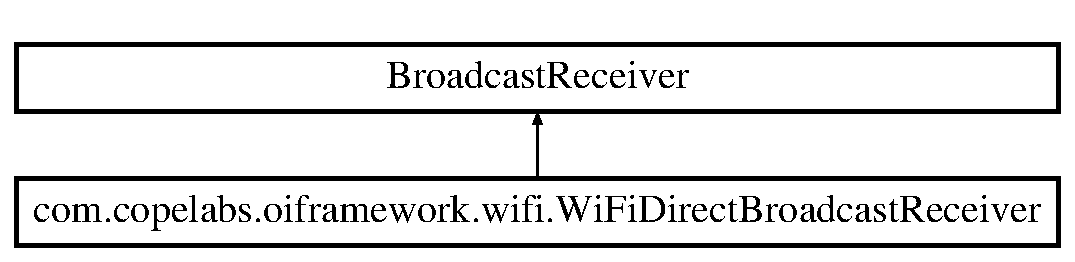
\includegraphics[height=2.000000cm]{classcom_1_1copelabs_1_1oiframework_1_1wifi_1_1_wi_fi_direct_broadcast_receiver}
\end{center}
\end{figure}
\subsection*{Public Member Functions}
\begin{DoxyCompactItemize}
\item 
\hyperlink{classcom_1_1copelabs_1_1oiframework_1_1wifi_1_1_wi_fi_direct_broadcast_receiver_a0f137949e21d30ee4bd03fc644eac9f6}{Wi\+Fi\+Direct\+Broadcast\+Receiver} (Wifi\+P2p\+Manager \hyperlink{classcom_1_1copelabs_1_1oiframework_1_1wifi_1_1_wi_fi_direct_broadcast_receiver_a2edba703acb8c53fdc2240bcc7e9335d}{manager}, Channel \hyperlink{classcom_1_1copelabs_1_1oiframework_1_1wifi_1_1_wi_fi_direct_broadcast_receiver_a473acb917add689a28682aa22cee8237}{channel}, \hyperlink{classcom_1_1copelabs_1_1oiframework_1_1wifi_1_1_wi_fi_direct_utils}{Wi\+Fi\+Direct\+Utils} \hyperlink{classcom_1_1copelabs_1_1oiframework_1_1wifi_1_1_wi_fi_direct_broadcast_receiver_a1a6dfa8aeb56af5456fc35250c9ddaee}{m\+Wi\+Fi\+Direct\+Utils})
\item 
void \hyperlink{classcom_1_1copelabs_1_1oiframework_1_1wifi_1_1_wi_fi_direct_broadcast_receiver_a126cb061d1fa1ba0fdd6fa9b4726f7bb}{on\+Receive} (Context context, Intent intent)
\end{DoxyCompactItemize}
\subsection*{Private Attributes}
\begin{DoxyCompactItemize}
\item 
Wifi\+P2p\+Manager \hyperlink{classcom_1_1copelabs_1_1oiframework_1_1wifi_1_1_wi_fi_direct_broadcast_receiver_a2edba703acb8c53fdc2240bcc7e9335d}{manager}
\item 
Channel \hyperlink{classcom_1_1copelabs_1_1oiframework_1_1wifi_1_1_wi_fi_direct_broadcast_receiver_a473acb917add689a28682aa22cee8237}{channel}
\item 
\hyperlink{classcom_1_1copelabs_1_1oiframework_1_1wifi_1_1_wi_fi_direct_utils}{Wi\+Fi\+Direct\+Utils} \hyperlink{classcom_1_1copelabs_1_1oiframework_1_1wifi_1_1_wi_fi_direct_broadcast_receiver_a1a6dfa8aeb56af5456fc35250c9ddaee}{m\+Wi\+Fi\+Direct\+Utils}
\end{DoxyCompactItemize}


\subsection{Detailed Description}
A Broadcast\+Receiver that notifies of important wifi p2p events. 

\subsection{Constructor \& Destructor Documentation}
\hypertarget{classcom_1_1copelabs_1_1oiframework_1_1wifi_1_1_wi_fi_direct_broadcast_receiver_a0f137949e21d30ee4bd03fc644eac9f6}{}\index{com\+::copelabs\+::oiframework\+::wifi\+::\+Wi\+Fi\+Direct\+Broadcast\+Receiver@{com\+::copelabs\+::oiframework\+::wifi\+::\+Wi\+Fi\+Direct\+Broadcast\+Receiver}!Wi\+Fi\+Direct\+Broadcast\+Receiver@{Wi\+Fi\+Direct\+Broadcast\+Receiver}}
\index{Wi\+Fi\+Direct\+Broadcast\+Receiver@{Wi\+Fi\+Direct\+Broadcast\+Receiver}!com\+::copelabs\+::oiframework\+::wifi\+::\+Wi\+Fi\+Direct\+Broadcast\+Receiver@{com\+::copelabs\+::oiframework\+::wifi\+::\+Wi\+Fi\+Direct\+Broadcast\+Receiver}}
\subsubsection[{Wi\+Fi\+Direct\+Broadcast\+Receiver(\+Wifi\+P2p\+Manager manager, Channel channel, Wi\+Fi\+Direct\+Utils m\+Wi\+Fi\+Direct\+Utils)}]{\setlength{\rightskip}{0pt plus 5cm}com.\+copelabs.\+oiframework.\+wifi.\+Wi\+Fi\+Direct\+Broadcast\+Receiver.\+Wi\+Fi\+Direct\+Broadcast\+Receiver (
\begin{DoxyParamCaption}
\item[{Wifi\+P2p\+Manager}]{manager, }
\item[{Channel}]{channel, }
\item[{{\bf Wi\+Fi\+Direct\+Utils}}]{m\+Wi\+Fi\+Direct\+Utils}
\end{DoxyParamCaption}
)}\label{classcom_1_1copelabs_1_1oiframework_1_1wifi_1_1_wi_fi_direct_broadcast_receiver_a0f137949e21d30ee4bd03fc644eac9f6}

\begin{DoxyParams}{Parameters}
{\em manager} & Wifi\+P2p\+Manager system service \\
\hline
{\em channel} & Wifi p2p channel \\
\hline
{\em activity} & activity associated with the receiver \\
\hline
\end{DoxyParams}


\subsection{Member Function Documentation}
\hypertarget{classcom_1_1copelabs_1_1oiframework_1_1wifi_1_1_wi_fi_direct_broadcast_receiver_a126cb061d1fa1ba0fdd6fa9b4726f7bb}{}\index{com\+::copelabs\+::oiframework\+::wifi\+::\+Wi\+Fi\+Direct\+Broadcast\+Receiver@{com\+::copelabs\+::oiframework\+::wifi\+::\+Wi\+Fi\+Direct\+Broadcast\+Receiver}!on\+Receive@{on\+Receive}}
\index{on\+Receive@{on\+Receive}!com\+::copelabs\+::oiframework\+::wifi\+::\+Wi\+Fi\+Direct\+Broadcast\+Receiver@{com\+::copelabs\+::oiframework\+::wifi\+::\+Wi\+Fi\+Direct\+Broadcast\+Receiver}}
\subsubsection[{on\+Receive(\+Context context, Intent intent)}]{\setlength{\rightskip}{0pt plus 5cm}void com.\+copelabs.\+oiframework.\+wifi.\+Wi\+Fi\+Direct\+Broadcast\+Receiver.\+on\+Receive (
\begin{DoxyParamCaption}
\item[{Context}]{context, }
\item[{Intent}]{intent}
\end{DoxyParamCaption}
)}\label{classcom_1_1copelabs_1_1oiframework_1_1wifi_1_1_wi_fi_direct_broadcast_receiver_a126cb061d1fa1ba0fdd6fa9b4726f7bb}


\subsection{Member Data Documentation}
\hypertarget{classcom_1_1copelabs_1_1oiframework_1_1wifi_1_1_wi_fi_direct_broadcast_receiver_a473acb917add689a28682aa22cee8237}{}\index{com\+::copelabs\+::oiframework\+::wifi\+::\+Wi\+Fi\+Direct\+Broadcast\+Receiver@{com\+::copelabs\+::oiframework\+::wifi\+::\+Wi\+Fi\+Direct\+Broadcast\+Receiver}!channel@{channel}}
\index{channel@{channel}!com\+::copelabs\+::oiframework\+::wifi\+::\+Wi\+Fi\+Direct\+Broadcast\+Receiver@{com\+::copelabs\+::oiframework\+::wifi\+::\+Wi\+Fi\+Direct\+Broadcast\+Receiver}}
\subsubsection[{channel}]{\setlength{\rightskip}{0pt plus 5cm}Channel com.\+copelabs.\+oiframework.\+wifi.\+Wi\+Fi\+Direct\+Broadcast\+Receiver.\+channel\hspace{0.3cm}{\ttfamily [private]}}\label{classcom_1_1copelabs_1_1oiframework_1_1wifi_1_1_wi_fi_direct_broadcast_receiver_a473acb917add689a28682aa22cee8237}
\hypertarget{classcom_1_1copelabs_1_1oiframework_1_1wifi_1_1_wi_fi_direct_broadcast_receiver_a2edba703acb8c53fdc2240bcc7e9335d}{}\index{com\+::copelabs\+::oiframework\+::wifi\+::\+Wi\+Fi\+Direct\+Broadcast\+Receiver@{com\+::copelabs\+::oiframework\+::wifi\+::\+Wi\+Fi\+Direct\+Broadcast\+Receiver}!manager@{manager}}
\index{manager@{manager}!com\+::copelabs\+::oiframework\+::wifi\+::\+Wi\+Fi\+Direct\+Broadcast\+Receiver@{com\+::copelabs\+::oiframework\+::wifi\+::\+Wi\+Fi\+Direct\+Broadcast\+Receiver}}
\subsubsection[{manager}]{\setlength{\rightskip}{0pt plus 5cm}Wifi\+P2p\+Manager com.\+copelabs.\+oiframework.\+wifi.\+Wi\+Fi\+Direct\+Broadcast\+Receiver.\+manager\hspace{0.3cm}{\ttfamily [private]}}\label{classcom_1_1copelabs_1_1oiframework_1_1wifi_1_1_wi_fi_direct_broadcast_receiver_a2edba703acb8c53fdc2240bcc7e9335d}
\hypertarget{classcom_1_1copelabs_1_1oiframework_1_1wifi_1_1_wi_fi_direct_broadcast_receiver_a1a6dfa8aeb56af5456fc35250c9ddaee}{}\index{com\+::copelabs\+::oiframework\+::wifi\+::\+Wi\+Fi\+Direct\+Broadcast\+Receiver@{com\+::copelabs\+::oiframework\+::wifi\+::\+Wi\+Fi\+Direct\+Broadcast\+Receiver}!m\+Wi\+Fi\+Direct\+Utils@{m\+Wi\+Fi\+Direct\+Utils}}
\index{m\+Wi\+Fi\+Direct\+Utils@{m\+Wi\+Fi\+Direct\+Utils}!com\+::copelabs\+::oiframework\+::wifi\+::\+Wi\+Fi\+Direct\+Broadcast\+Receiver@{com\+::copelabs\+::oiframework\+::wifi\+::\+Wi\+Fi\+Direct\+Broadcast\+Receiver}}
\subsubsection[{m\+Wi\+Fi\+Direct\+Utils}]{\setlength{\rightskip}{0pt plus 5cm}{\bf Wi\+Fi\+Direct\+Utils} com.\+copelabs.\+oiframework.\+wifi.\+Wi\+Fi\+Direct\+Broadcast\+Receiver.\+m\+Wi\+Fi\+Direct\+Utils\hspace{0.3cm}{\ttfamily [private]}}\label{classcom_1_1copelabs_1_1oiframework_1_1wifi_1_1_wi_fi_direct_broadcast_receiver_a1a6dfa8aeb56af5456fc35250c9ddaee}


The documentation for this class was generated from the following file\+:\begin{DoxyCompactItemize}
\item 
src/com/copelabs/oiframework/wifi/\hyperlink{_wi_fi_direct_broadcast_receiver_8java}{Wi\+Fi\+Direct\+Broadcast\+Receiver.\+java}\end{DoxyCompactItemize}

\hypertarget{classcom_1_1copelabs_1_1oiframework_1_1wifi_1_1_wi_fi_direct_device}{}\section{com.\+copelabs.\+oiframework.\+wifi.\+Wi\+Fi\+Direct\+Device Class Reference}
\label{classcom_1_1copelabs_1_1oiframework_1_1wifi_1_1_wi_fi_direct_device}\index{com.\+copelabs.\+oiframework.\+wifi.\+Wi\+Fi\+Direct\+Device@{com.\+copelabs.\+oiframework.\+wifi.\+Wi\+Fi\+Direct\+Device}}
\subsection*{Public Member Functions}
\begin{DoxyCompactItemize}
\item 
\hyperlink{classcom_1_1copelabs_1_1oiframework_1_1wifi_1_1_wi_fi_direct_device_a7bd474414b2e79e3319b2147e7288bd7}{Wi\+Fi\+Direct\+Device} ()
\item 
void \hyperlink{classcom_1_1copelabs_1_1oiframework_1_1wifi_1_1_wi_fi_direct_device_a279aa058cc7be37d1111d4830f80be71}{set\+Device} (Wifi\+P2p\+Device \hyperlink{classcom_1_1copelabs_1_1oiframework_1_1wifi_1_1_wi_fi_direct_device_ae8eb9ce4fe61f8816bc1d782920c3062}{device})
\item 
void \hyperlink{classcom_1_1copelabs_1_1oiframework_1_1wifi_1_1_wi_fi_direct_device_af38ebd62b4bdf2c1f3f5da5061c64c26}{set\+Instance\+Name} (String \hyperlink{classcom_1_1copelabs_1_1oiframework_1_1wifi_1_1_wi_fi_direct_device_a777116482205bdc4277dd67b97eb759e}{instance\+Name})
\item 
void \hyperlink{classcom_1_1copelabs_1_1oiframework_1_1wifi_1_1_wi_fi_direct_device_a58ac586803a114d87a269951168df8df}{set\+Service\+Registration\+Type} (String \hyperlink{classcom_1_1copelabs_1_1oiframework_1_1wifi_1_1_wi_fi_direct_device_a53d05b7aa0924e76b0c2b567affb1112}{service\+Registration\+Type})
\item 
void \hyperlink{classcom_1_1copelabs_1_1oiframework_1_1wifi_1_1_wi_fi_direct_device_adeabc501f12f316bec96f5955f3c7ad5}{set\+Last\+Time\+Seen} (long m\+Time)
\item 
Wifi\+P2p\+Device \hyperlink{classcom_1_1copelabs_1_1oiframework_1_1wifi_1_1_wi_fi_direct_device_ae967d6513dc4b32e22e75a15a2f2e041}{get\+Device} ()
\item 
String \hyperlink{classcom_1_1copelabs_1_1oiframework_1_1wifi_1_1_wi_fi_direct_device_a98d80ea23930328f27f430cf60918540}{get\+Instance\+Name} ()
\item 
String \hyperlink{classcom_1_1copelabs_1_1oiframework_1_1wifi_1_1_wi_fi_direct_device_adcb8042f950497d18987766e7c0b9b81}{get\+Service\+Registration\+Type} ()
\item 
long \hyperlink{classcom_1_1copelabs_1_1oiframework_1_1wifi_1_1_wi_fi_direct_device_ac7dc2702eaac0636f254580f3ce3282e}{get\+Last\+Time\+Seen} ()
\end{DoxyCompactItemize}
\subsection*{Private Attributes}
\begin{DoxyCompactItemize}
\item 
Wifi\+P2p\+Device \hyperlink{classcom_1_1copelabs_1_1oiframework_1_1wifi_1_1_wi_fi_direct_device_ae8eb9ce4fe61f8816bc1d782920c3062}{device}
\item 
String \hyperlink{classcom_1_1copelabs_1_1oiframework_1_1wifi_1_1_wi_fi_direct_device_a777116482205bdc4277dd67b97eb759e}{instance\+Name} = null
\item 
String \hyperlink{classcom_1_1copelabs_1_1oiframework_1_1wifi_1_1_wi_fi_direct_device_a53d05b7aa0924e76b0c2b567affb1112}{service\+Registration\+Type} = null
\item 
long \hyperlink{classcom_1_1copelabs_1_1oiframework_1_1wifi_1_1_wi_fi_direct_device_aedc5d49186dfa466662e225490009b2c}{T\+T\+L}
\end{DoxyCompactItemize}


\subsection{Detailed Description}
A structure to hold service information. 

\subsection{Constructor \& Destructor Documentation}
\hypertarget{classcom_1_1copelabs_1_1oiframework_1_1wifi_1_1_wi_fi_direct_device_a7bd474414b2e79e3319b2147e7288bd7}{}\index{com\+::copelabs\+::oiframework\+::wifi\+::\+Wi\+Fi\+Direct\+Device@{com\+::copelabs\+::oiframework\+::wifi\+::\+Wi\+Fi\+Direct\+Device}!Wi\+Fi\+Direct\+Device@{Wi\+Fi\+Direct\+Device}}
\index{Wi\+Fi\+Direct\+Device@{Wi\+Fi\+Direct\+Device}!com\+::copelabs\+::oiframework\+::wifi\+::\+Wi\+Fi\+Direct\+Device@{com\+::copelabs\+::oiframework\+::wifi\+::\+Wi\+Fi\+Direct\+Device}}
\subsubsection[{Wi\+Fi\+Direct\+Device()}]{\setlength{\rightskip}{0pt plus 5cm}com.\+copelabs.\+oiframework.\+wifi.\+Wi\+Fi\+Direct\+Device.\+Wi\+Fi\+Direct\+Device (
\begin{DoxyParamCaption}
{}
\end{DoxyParamCaption}
)}\label{classcom_1_1copelabs_1_1oiframework_1_1wifi_1_1_wi_fi_direct_device_a7bd474414b2e79e3319b2147e7288bd7}


\subsection{Member Function Documentation}
\hypertarget{classcom_1_1copelabs_1_1oiframework_1_1wifi_1_1_wi_fi_direct_device_ae967d6513dc4b32e22e75a15a2f2e041}{}\index{com\+::copelabs\+::oiframework\+::wifi\+::\+Wi\+Fi\+Direct\+Device@{com\+::copelabs\+::oiframework\+::wifi\+::\+Wi\+Fi\+Direct\+Device}!get\+Device@{get\+Device}}
\index{get\+Device@{get\+Device}!com\+::copelabs\+::oiframework\+::wifi\+::\+Wi\+Fi\+Direct\+Device@{com\+::copelabs\+::oiframework\+::wifi\+::\+Wi\+Fi\+Direct\+Device}}
\subsubsection[{get\+Device()}]{\setlength{\rightskip}{0pt plus 5cm}Wifi\+P2p\+Device com.\+copelabs.\+oiframework.\+wifi.\+Wi\+Fi\+Direct\+Device.\+get\+Device (
\begin{DoxyParamCaption}
{}
\end{DoxyParamCaption}
)}\label{classcom_1_1copelabs_1_1oiframework_1_1wifi_1_1_wi_fi_direct_device_ae967d6513dc4b32e22e75a15a2f2e041}
\hypertarget{classcom_1_1copelabs_1_1oiframework_1_1wifi_1_1_wi_fi_direct_device_a98d80ea23930328f27f430cf60918540}{}\index{com\+::copelabs\+::oiframework\+::wifi\+::\+Wi\+Fi\+Direct\+Device@{com\+::copelabs\+::oiframework\+::wifi\+::\+Wi\+Fi\+Direct\+Device}!get\+Instance\+Name@{get\+Instance\+Name}}
\index{get\+Instance\+Name@{get\+Instance\+Name}!com\+::copelabs\+::oiframework\+::wifi\+::\+Wi\+Fi\+Direct\+Device@{com\+::copelabs\+::oiframework\+::wifi\+::\+Wi\+Fi\+Direct\+Device}}
\subsubsection[{get\+Instance\+Name()}]{\setlength{\rightskip}{0pt plus 5cm}String com.\+copelabs.\+oiframework.\+wifi.\+Wi\+Fi\+Direct\+Device.\+get\+Instance\+Name (
\begin{DoxyParamCaption}
{}
\end{DoxyParamCaption}
)}\label{classcom_1_1copelabs_1_1oiframework_1_1wifi_1_1_wi_fi_direct_device_a98d80ea23930328f27f430cf60918540}
\hypertarget{classcom_1_1copelabs_1_1oiframework_1_1wifi_1_1_wi_fi_direct_device_ac7dc2702eaac0636f254580f3ce3282e}{}\index{com\+::copelabs\+::oiframework\+::wifi\+::\+Wi\+Fi\+Direct\+Device@{com\+::copelabs\+::oiframework\+::wifi\+::\+Wi\+Fi\+Direct\+Device}!get\+Last\+Time\+Seen@{get\+Last\+Time\+Seen}}
\index{get\+Last\+Time\+Seen@{get\+Last\+Time\+Seen}!com\+::copelabs\+::oiframework\+::wifi\+::\+Wi\+Fi\+Direct\+Device@{com\+::copelabs\+::oiframework\+::wifi\+::\+Wi\+Fi\+Direct\+Device}}
\subsubsection[{get\+Last\+Time\+Seen()}]{\setlength{\rightskip}{0pt plus 5cm}long com.\+copelabs.\+oiframework.\+wifi.\+Wi\+Fi\+Direct\+Device.\+get\+Last\+Time\+Seen (
\begin{DoxyParamCaption}
{}
\end{DoxyParamCaption}
)}\label{classcom_1_1copelabs_1_1oiframework_1_1wifi_1_1_wi_fi_direct_device_ac7dc2702eaac0636f254580f3ce3282e}
\hypertarget{classcom_1_1copelabs_1_1oiframework_1_1wifi_1_1_wi_fi_direct_device_adcb8042f950497d18987766e7c0b9b81}{}\index{com\+::copelabs\+::oiframework\+::wifi\+::\+Wi\+Fi\+Direct\+Device@{com\+::copelabs\+::oiframework\+::wifi\+::\+Wi\+Fi\+Direct\+Device}!get\+Service\+Registration\+Type@{get\+Service\+Registration\+Type}}
\index{get\+Service\+Registration\+Type@{get\+Service\+Registration\+Type}!com\+::copelabs\+::oiframework\+::wifi\+::\+Wi\+Fi\+Direct\+Device@{com\+::copelabs\+::oiframework\+::wifi\+::\+Wi\+Fi\+Direct\+Device}}
\subsubsection[{get\+Service\+Registration\+Type()}]{\setlength{\rightskip}{0pt plus 5cm}String com.\+copelabs.\+oiframework.\+wifi.\+Wi\+Fi\+Direct\+Device.\+get\+Service\+Registration\+Type (
\begin{DoxyParamCaption}
{}
\end{DoxyParamCaption}
)}\label{classcom_1_1copelabs_1_1oiframework_1_1wifi_1_1_wi_fi_direct_device_adcb8042f950497d18987766e7c0b9b81}
\hypertarget{classcom_1_1copelabs_1_1oiframework_1_1wifi_1_1_wi_fi_direct_device_a279aa058cc7be37d1111d4830f80be71}{}\index{com\+::copelabs\+::oiframework\+::wifi\+::\+Wi\+Fi\+Direct\+Device@{com\+::copelabs\+::oiframework\+::wifi\+::\+Wi\+Fi\+Direct\+Device}!set\+Device@{set\+Device}}
\index{set\+Device@{set\+Device}!com\+::copelabs\+::oiframework\+::wifi\+::\+Wi\+Fi\+Direct\+Device@{com\+::copelabs\+::oiframework\+::wifi\+::\+Wi\+Fi\+Direct\+Device}}
\subsubsection[{set\+Device(\+Wifi\+P2p\+Device device)}]{\setlength{\rightskip}{0pt plus 5cm}void com.\+copelabs.\+oiframework.\+wifi.\+Wi\+Fi\+Direct\+Device.\+set\+Device (
\begin{DoxyParamCaption}
\item[{Wifi\+P2p\+Device}]{device}
\end{DoxyParamCaption}
)}\label{classcom_1_1copelabs_1_1oiframework_1_1wifi_1_1_wi_fi_direct_device_a279aa058cc7be37d1111d4830f80be71}
\hypertarget{classcom_1_1copelabs_1_1oiframework_1_1wifi_1_1_wi_fi_direct_device_af38ebd62b4bdf2c1f3f5da5061c64c26}{}\index{com\+::copelabs\+::oiframework\+::wifi\+::\+Wi\+Fi\+Direct\+Device@{com\+::copelabs\+::oiframework\+::wifi\+::\+Wi\+Fi\+Direct\+Device}!set\+Instance\+Name@{set\+Instance\+Name}}
\index{set\+Instance\+Name@{set\+Instance\+Name}!com\+::copelabs\+::oiframework\+::wifi\+::\+Wi\+Fi\+Direct\+Device@{com\+::copelabs\+::oiframework\+::wifi\+::\+Wi\+Fi\+Direct\+Device}}
\subsubsection[{set\+Instance\+Name(\+String instance\+Name)}]{\setlength{\rightskip}{0pt plus 5cm}void com.\+copelabs.\+oiframework.\+wifi.\+Wi\+Fi\+Direct\+Device.\+set\+Instance\+Name (
\begin{DoxyParamCaption}
\item[{String}]{instance\+Name}
\end{DoxyParamCaption}
)}\label{classcom_1_1copelabs_1_1oiframework_1_1wifi_1_1_wi_fi_direct_device_af38ebd62b4bdf2c1f3f5da5061c64c26}
\hypertarget{classcom_1_1copelabs_1_1oiframework_1_1wifi_1_1_wi_fi_direct_device_adeabc501f12f316bec96f5955f3c7ad5}{}\index{com\+::copelabs\+::oiframework\+::wifi\+::\+Wi\+Fi\+Direct\+Device@{com\+::copelabs\+::oiframework\+::wifi\+::\+Wi\+Fi\+Direct\+Device}!set\+Last\+Time\+Seen@{set\+Last\+Time\+Seen}}
\index{set\+Last\+Time\+Seen@{set\+Last\+Time\+Seen}!com\+::copelabs\+::oiframework\+::wifi\+::\+Wi\+Fi\+Direct\+Device@{com\+::copelabs\+::oiframework\+::wifi\+::\+Wi\+Fi\+Direct\+Device}}
\subsubsection[{set\+Last\+Time\+Seen(long m\+Time)}]{\setlength{\rightskip}{0pt plus 5cm}void com.\+copelabs.\+oiframework.\+wifi.\+Wi\+Fi\+Direct\+Device.\+set\+Last\+Time\+Seen (
\begin{DoxyParamCaption}
\item[{long}]{m\+Time}
\end{DoxyParamCaption}
)}\label{classcom_1_1copelabs_1_1oiframework_1_1wifi_1_1_wi_fi_direct_device_adeabc501f12f316bec96f5955f3c7ad5}
\hypertarget{classcom_1_1copelabs_1_1oiframework_1_1wifi_1_1_wi_fi_direct_device_a58ac586803a114d87a269951168df8df}{}\index{com\+::copelabs\+::oiframework\+::wifi\+::\+Wi\+Fi\+Direct\+Device@{com\+::copelabs\+::oiframework\+::wifi\+::\+Wi\+Fi\+Direct\+Device}!set\+Service\+Registration\+Type@{set\+Service\+Registration\+Type}}
\index{set\+Service\+Registration\+Type@{set\+Service\+Registration\+Type}!com\+::copelabs\+::oiframework\+::wifi\+::\+Wi\+Fi\+Direct\+Device@{com\+::copelabs\+::oiframework\+::wifi\+::\+Wi\+Fi\+Direct\+Device}}
\subsubsection[{set\+Service\+Registration\+Type(\+String service\+Registration\+Type)}]{\setlength{\rightskip}{0pt plus 5cm}void com.\+copelabs.\+oiframework.\+wifi.\+Wi\+Fi\+Direct\+Device.\+set\+Service\+Registration\+Type (
\begin{DoxyParamCaption}
\item[{String}]{service\+Registration\+Type}
\end{DoxyParamCaption}
)}\label{classcom_1_1copelabs_1_1oiframework_1_1wifi_1_1_wi_fi_direct_device_a58ac586803a114d87a269951168df8df}


\subsection{Member Data Documentation}
\hypertarget{classcom_1_1copelabs_1_1oiframework_1_1wifi_1_1_wi_fi_direct_device_ae8eb9ce4fe61f8816bc1d782920c3062}{}\index{com\+::copelabs\+::oiframework\+::wifi\+::\+Wi\+Fi\+Direct\+Device@{com\+::copelabs\+::oiframework\+::wifi\+::\+Wi\+Fi\+Direct\+Device}!device@{device}}
\index{device@{device}!com\+::copelabs\+::oiframework\+::wifi\+::\+Wi\+Fi\+Direct\+Device@{com\+::copelabs\+::oiframework\+::wifi\+::\+Wi\+Fi\+Direct\+Device}}
\subsubsection[{device}]{\setlength{\rightskip}{0pt plus 5cm}Wifi\+P2p\+Device com.\+copelabs.\+oiframework.\+wifi.\+Wi\+Fi\+Direct\+Device.\+device\hspace{0.3cm}{\ttfamily [private]}}\label{classcom_1_1copelabs_1_1oiframework_1_1wifi_1_1_wi_fi_direct_device_ae8eb9ce4fe61f8816bc1d782920c3062}
\hypertarget{classcom_1_1copelabs_1_1oiframework_1_1wifi_1_1_wi_fi_direct_device_a777116482205bdc4277dd67b97eb759e}{}\index{com\+::copelabs\+::oiframework\+::wifi\+::\+Wi\+Fi\+Direct\+Device@{com\+::copelabs\+::oiframework\+::wifi\+::\+Wi\+Fi\+Direct\+Device}!instance\+Name@{instance\+Name}}
\index{instance\+Name@{instance\+Name}!com\+::copelabs\+::oiframework\+::wifi\+::\+Wi\+Fi\+Direct\+Device@{com\+::copelabs\+::oiframework\+::wifi\+::\+Wi\+Fi\+Direct\+Device}}
\subsubsection[{instance\+Name}]{\setlength{\rightskip}{0pt plus 5cm}String com.\+copelabs.\+oiframework.\+wifi.\+Wi\+Fi\+Direct\+Device.\+instance\+Name = null\hspace{0.3cm}{\ttfamily [private]}}\label{classcom_1_1copelabs_1_1oiframework_1_1wifi_1_1_wi_fi_direct_device_a777116482205bdc4277dd67b97eb759e}
\hypertarget{classcom_1_1copelabs_1_1oiframework_1_1wifi_1_1_wi_fi_direct_device_a53d05b7aa0924e76b0c2b567affb1112}{}\index{com\+::copelabs\+::oiframework\+::wifi\+::\+Wi\+Fi\+Direct\+Device@{com\+::copelabs\+::oiframework\+::wifi\+::\+Wi\+Fi\+Direct\+Device}!service\+Registration\+Type@{service\+Registration\+Type}}
\index{service\+Registration\+Type@{service\+Registration\+Type}!com\+::copelabs\+::oiframework\+::wifi\+::\+Wi\+Fi\+Direct\+Device@{com\+::copelabs\+::oiframework\+::wifi\+::\+Wi\+Fi\+Direct\+Device}}
\subsubsection[{service\+Registration\+Type}]{\setlength{\rightskip}{0pt plus 5cm}String com.\+copelabs.\+oiframework.\+wifi.\+Wi\+Fi\+Direct\+Device.\+service\+Registration\+Type = null\hspace{0.3cm}{\ttfamily [private]}}\label{classcom_1_1copelabs_1_1oiframework_1_1wifi_1_1_wi_fi_direct_device_a53d05b7aa0924e76b0c2b567affb1112}
\hypertarget{classcom_1_1copelabs_1_1oiframework_1_1wifi_1_1_wi_fi_direct_device_aedc5d49186dfa466662e225490009b2c}{}\index{com\+::copelabs\+::oiframework\+::wifi\+::\+Wi\+Fi\+Direct\+Device@{com\+::copelabs\+::oiframework\+::wifi\+::\+Wi\+Fi\+Direct\+Device}!T\+T\+L@{T\+T\+L}}
\index{T\+T\+L@{T\+T\+L}!com\+::copelabs\+::oiframework\+::wifi\+::\+Wi\+Fi\+Direct\+Device@{com\+::copelabs\+::oiframework\+::wifi\+::\+Wi\+Fi\+Direct\+Device}}
\subsubsection[{T\+T\+L}]{\setlength{\rightskip}{0pt plus 5cm}long com.\+copelabs.\+oiframework.\+wifi.\+Wi\+Fi\+Direct\+Device.\+T\+T\+L\hspace{0.3cm}{\ttfamily [private]}}\label{classcom_1_1copelabs_1_1oiframework_1_1wifi_1_1_wi_fi_direct_device_aedc5d49186dfa466662e225490009b2c}


The documentation for this class was generated from the following file\+:\begin{DoxyCompactItemize}
\item 
src/com/copelabs/oiframework/wifi/\hyperlink{_wi_fi_direct_device_8java}{Wi\+Fi\+Direct\+Device.\+java}\end{DoxyCompactItemize}

\hypertarget{interfacecom_1_1copelabs_1_1oiframework_1_1wifi_1_1_wi_fi_direct_listener}{}\section{com.\+copelabs.\+oiframework.\+wifi.\+Wi\+Fi\+Direct\+Listener Interface Reference}
\label{interfacecom_1_1copelabs_1_1oiframework_1_1wifi_1_1_wi_fi_direct_listener}\index{com.\+copelabs.\+oiframework.\+wifi.\+Wi\+Fi\+Direct\+Listener@{com.\+copelabs.\+oiframework.\+wifi.\+Wi\+Fi\+Direct\+Listener}}
\subsection*{Public Member Functions}
\begin{DoxyCompactItemize}
\item 
void \hyperlink{interfacecom_1_1copelabs_1_1oiframework_1_1wifi_1_1_wi_fi_direct_listener_ab02f5ae14a0bab182bcfd6d0c226cfd6}{on\+Packet\+Received} (List$<$ \hyperlink{classcom_1_1copelabs_1_1oiframework_1_1contentmanager_1_1_packet}{Packet} $>$ m\+List\+Of\+Packets)
\item 
void \hyperlink{interfacecom_1_1copelabs_1_1oiframework_1_1wifi_1_1_wi_fi_direct_listener_a1ac8d66511dc1152ffd9d404c2acb66a}{on\+New\+Wi\+Fi\+Direct\+Device\+Found} (\hyperlink{classcom_1_1copelabs_1_1oiframework_1_1wifi_1_1_wi_fi_direct_device}{Wi\+Fi\+Direct\+Device} m\+Device, Map$<$ String, String $>$ m\+List\+Of\+Social\+Weight)
\item 
void \hyperlink{interfacecom_1_1copelabs_1_1oiframework_1_1wifi_1_1_wi_fi_direct_listener_a119dc7b314e02166bfeeb6b45f9b6a51}{on\+Wi\+Fi\+Direct\+Device\+Disappear} (\hyperlink{classcom_1_1copelabs_1_1oiframework_1_1wifi_1_1_wi_fi_direct_device}{Wi\+Fi\+Direct\+Device} m\+Device)
\item 
void \hyperlink{interfacecom_1_1copelabs_1_1oiframework_1_1wifi_1_1_wi_fi_direct_listener_a1c2013553cc66064055c1015f59a7198}{error} (int m\+Error)
\end{DoxyCompactItemize}


\subsection{Member Function Documentation}
\hypertarget{interfacecom_1_1copelabs_1_1oiframework_1_1wifi_1_1_wi_fi_direct_listener_a1c2013553cc66064055c1015f59a7198}{}\index{com\+::copelabs\+::oiframework\+::wifi\+::\+Wi\+Fi\+Direct\+Listener@{com\+::copelabs\+::oiframework\+::wifi\+::\+Wi\+Fi\+Direct\+Listener}!error@{error}}
\index{error@{error}!com\+::copelabs\+::oiframework\+::wifi\+::\+Wi\+Fi\+Direct\+Listener@{com\+::copelabs\+::oiframework\+::wifi\+::\+Wi\+Fi\+Direct\+Listener}}
\subsubsection[{error(int m\+Error)}]{\setlength{\rightskip}{0pt plus 5cm}void com.\+copelabs.\+oiframework.\+wifi.\+Wi\+Fi\+Direct\+Listener.\+error (
\begin{DoxyParamCaption}
\item[{int}]{m\+Error}
\end{DoxyParamCaption}
)}\label{interfacecom_1_1copelabs_1_1oiframework_1_1wifi_1_1_wi_fi_direct_listener_a1c2013553cc66064055c1015f59a7198}
\hypertarget{interfacecom_1_1copelabs_1_1oiframework_1_1wifi_1_1_wi_fi_direct_listener_a1ac8d66511dc1152ffd9d404c2acb66a}{}\index{com\+::copelabs\+::oiframework\+::wifi\+::\+Wi\+Fi\+Direct\+Listener@{com\+::copelabs\+::oiframework\+::wifi\+::\+Wi\+Fi\+Direct\+Listener}!on\+New\+Wi\+Fi\+Direct\+Device\+Found@{on\+New\+Wi\+Fi\+Direct\+Device\+Found}}
\index{on\+New\+Wi\+Fi\+Direct\+Device\+Found@{on\+New\+Wi\+Fi\+Direct\+Device\+Found}!com\+::copelabs\+::oiframework\+::wifi\+::\+Wi\+Fi\+Direct\+Listener@{com\+::copelabs\+::oiframework\+::wifi\+::\+Wi\+Fi\+Direct\+Listener}}
\subsubsection[{on\+New\+Wi\+Fi\+Direct\+Device\+Found(\+Wi\+Fi\+Direct\+Device m\+Device, Map$<$ String, String $>$ m\+List\+Of\+Social\+Weight)}]{\setlength{\rightskip}{0pt plus 5cm}void com.\+copelabs.\+oiframework.\+wifi.\+Wi\+Fi\+Direct\+Listener.\+on\+New\+Wi\+Fi\+Direct\+Device\+Found (
\begin{DoxyParamCaption}
\item[{{\bf Wi\+Fi\+Direct\+Device}}]{m\+Device, }
\item[{Map$<$ String, String $>$}]{m\+List\+Of\+Social\+Weight}
\end{DoxyParamCaption}
)}\label{interfacecom_1_1copelabs_1_1oiframework_1_1wifi_1_1_wi_fi_direct_listener_a1ac8d66511dc1152ffd9d404c2acb66a}
\hypertarget{interfacecom_1_1copelabs_1_1oiframework_1_1wifi_1_1_wi_fi_direct_listener_ab02f5ae14a0bab182bcfd6d0c226cfd6}{}\index{com\+::copelabs\+::oiframework\+::wifi\+::\+Wi\+Fi\+Direct\+Listener@{com\+::copelabs\+::oiframework\+::wifi\+::\+Wi\+Fi\+Direct\+Listener}!on\+Packet\+Received@{on\+Packet\+Received}}
\index{on\+Packet\+Received@{on\+Packet\+Received}!com\+::copelabs\+::oiframework\+::wifi\+::\+Wi\+Fi\+Direct\+Listener@{com\+::copelabs\+::oiframework\+::wifi\+::\+Wi\+Fi\+Direct\+Listener}}
\subsubsection[{on\+Packet\+Received(\+List$<$ Packet $>$ m\+List\+Of\+Packets)}]{\setlength{\rightskip}{0pt plus 5cm}void com.\+copelabs.\+oiframework.\+wifi.\+Wi\+Fi\+Direct\+Listener.\+on\+Packet\+Received (
\begin{DoxyParamCaption}
\item[{List$<$ {\bf Packet} $>$}]{m\+List\+Of\+Packets}
\end{DoxyParamCaption}
)}\label{interfacecom_1_1copelabs_1_1oiframework_1_1wifi_1_1_wi_fi_direct_listener_ab02f5ae14a0bab182bcfd6d0c226cfd6}
\hypertarget{interfacecom_1_1copelabs_1_1oiframework_1_1wifi_1_1_wi_fi_direct_listener_a119dc7b314e02166bfeeb6b45f9b6a51}{}\index{com\+::copelabs\+::oiframework\+::wifi\+::\+Wi\+Fi\+Direct\+Listener@{com\+::copelabs\+::oiframework\+::wifi\+::\+Wi\+Fi\+Direct\+Listener}!on\+Wi\+Fi\+Direct\+Device\+Disappear@{on\+Wi\+Fi\+Direct\+Device\+Disappear}}
\index{on\+Wi\+Fi\+Direct\+Device\+Disappear@{on\+Wi\+Fi\+Direct\+Device\+Disappear}!com\+::copelabs\+::oiframework\+::wifi\+::\+Wi\+Fi\+Direct\+Listener@{com\+::copelabs\+::oiframework\+::wifi\+::\+Wi\+Fi\+Direct\+Listener}}
\subsubsection[{on\+Wi\+Fi\+Direct\+Device\+Disappear(\+Wi\+Fi\+Direct\+Device m\+Device)}]{\setlength{\rightskip}{0pt plus 5cm}void com.\+copelabs.\+oiframework.\+wifi.\+Wi\+Fi\+Direct\+Listener.\+on\+Wi\+Fi\+Direct\+Device\+Disappear (
\begin{DoxyParamCaption}
\item[{{\bf Wi\+Fi\+Direct\+Device}}]{m\+Device}
\end{DoxyParamCaption}
)}\label{interfacecom_1_1copelabs_1_1oiframework_1_1wifi_1_1_wi_fi_direct_listener_a119dc7b314e02166bfeeb6b45f9b6a51}


The documentation for this interface was generated from the following file\+:\begin{DoxyCompactItemize}
\item 
src/com/copelabs/oiframework/wifi/\hyperlink{_wi_fi_direct_listener_8java}{Wi\+Fi\+Direct\+Listener.\+java}\end{DoxyCompactItemize}

\hypertarget{classcom_1_1copelabs_1_1oiframework_1_1wifi_1_1_wi_fi_direct_utils}{}\section{com.\+copelabs.\+oiframework.\+wifi.\+Wi\+Fi\+Direct\+Utils Class Reference}
\label{classcom_1_1copelabs_1_1oiframework_1_1wifi_1_1_wi_fi_direct_utils}\index{com.\+copelabs.\+oiframework.\+wifi.\+Wi\+Fi\+Direct\+Utils@{com.\+copelabs.\+oiframework.\+wifi.\+Wi\+Fi\+Direct\+Utils}}
Inheritance diagram for com.\+copelabs.\+oiframework.\+wifi.\+Wi\+Fi\+Direct\+Utils\+:\begin{figure}[H]
\begin{center}
\leavevmode
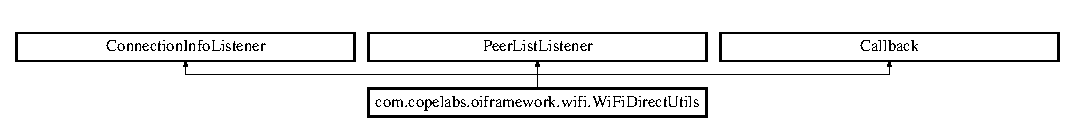
\includegraphics[height=1.333333cm]{classcom_1_1copelabs_1_1oiframework_1_1wifi_1_1_wi_fi_direct_utils}
\end{center}
\end{figure}
\subsection*{Public Member Functions}
\begin{DoxyCompactItemize}
\item 
\hyperlink{classcom_1_1copelabs_1_1oiframework_1_1wifi_1_1_wi_fi_direct_utils_aa781d8a3adc56542ef3a8ef675731158}{Wi\+Fi\+Direct\+Utils} (Context \hyperlink{classcom_1_1copelabs_1_1oiframework_1_1wifi_1_1_wi_fi_direct_utils_a7eb74c5567159ba6d78c824d290c07bb}{m\+Context}, \hyperlink{classcom_1_1copelabs_1_1oiframework_1_1wifi_1_1_wi_fi_direct}{Wi\+Fi\+Direct} \hyperlink{classcom_1_1copelabs_1_1oiframework_1_1wifi_1_1_wi_fi_direct_utils_af418801f7c19d45da15758d1bc249bff}{m\+Callback})
\item 
Handler \hyperlink{classcom_1_1copelabs_1_1oiframework_1_1wifi_1_1_wi_fi_direct_utils_a9b56b3303022e512107625b844f1d7d1}{get\+Handler} ()
\item 
void \hyperlink{classcom_1_1copelabs_1_1oiframework_1_1wifi_1_1_wi_fi_direct_utils_a17b28a093d6c475b0c18cae14bdb821c}{set\+Handler} (Handler \hyperlink{classcom_1_1copelabs_1_1oiframework_1_1wifi_1_1_wi_fi_direct_utils_af585a8ac857febc2ac01888cb7281db2}{handler})
\item 
void \hyperlink{classcom_1_1copelabs_1_1oiframework_1_1wifi_1_1_wi_fi_direct_utils_a4eead54248c89920a0be71cb7bf8b807}{set\+Is\+Wifi\+P2p\+Enabled} (boolean \hyperlink{classcom_1_1copelabs_1_1oiframework_1_1wifi_1_1_wi_fi_direct_utils_a77f5909127d477f0630858fe4f68df46}{is\+Wifi\+P2p\+Enabled})
\item 
boolean \hyperlink{classcom_1_1copelabs_1_1oiframework_1_1wifi_1_1_wi_fi_direct_utils_a8b76b8a077829299388b493d9e7e9cbb}{get\+Is\+Wifi\+P2p\+Enabled} ()
\item 
String \hyperlink{classcom_1_1copelabs_1_1oiframework_1_1wifi_1_1_wi_fi_direct_utils_ab4db03fbc9387b2f49002224171ca743}{get\+W\+F\+Direct\+Mac\+Address} ()
\item 
String \hyperlink{classcom_1_1copelabs_1_1oiframework_1_1wifi_1_1_wi_fi_direct_utils_ac93d53d24424cd39ea70b371b58b89b2}{get\+Wi\+Fi\+Mac\+Address} ()
\item 
void \hyperlink{classcom_1_1copelabs_1_1oiframework_1_1wifi_1_1_wi_fi_direct_utils_aaa6cf1b0d0105e6211e5bf7d9ec929b1}{start} (final String m\+M\+A\+C, final Map$<$ String, String $>$ m\+List\+Of\+Social\+Weight)
\item 
void \hyperlink{classcom_1_1copelabs_1_1oiframework_1_1wifi_1_1_wi_fi_direct_utils_a0903f28238740adb65d2cbbd5d9cc27b}{stop} ()
\item 
void \hyperlink{classcom_1_1copelabs_1_1oiframework_1_1wifi_1_1_wi_fi_direct_utils_ae61cb2338da82fbbbe9ed599f20d8c1f}{wifi\+Was\+Enabled} ()
\item 
void \hyperlink{classcom_1_1copelabs_1_1oiframework_1_1wifi_1_1_wi_fi_direct_utils_a20181b6d9ff64c44342865ae1c5580b4}{wifi\+Disabled} ()
\item 
void \hyperlink{classcom_1_1copelabs_1_1oiframework_1_1wifi_1_1_wi_fi_direct_utils_aef56711248db2c26e1647f757bf9b4d4}{restart\+Discovery} ()
\item 
void \hyperlink{classcom_1_1copelabs_1_1oiframework_1_1wifi_1_1_wi_fi_direct_utils_ae10f8c8c1a46e71bca770c9659469f32}{update\+Registration} (final String m\+M\+A\+C, final Map$<$ String, String $>$ m\+List\+Of\+Social\+Weight)
\item 
void \hyperlink{classcom_1_1copelabs_1_1oiframework_1_1wifi_1_1_wi_fi_direct_utils_a9f4a5e9253832b8956784d43e634fbd8}{discover\+Service} ()
\item 
void \hyperlink{classcom_1_1copelabs_1_1oiframework_1_1wifi_1_1_wi_fi_direct_utils_aa35c6d687a1f0724748230146d7e20dd}{on\+Peers\+Available} (Wifi\+P2p\+Device\+List peers)
\item 
boolean \hyperlink{classcom_1_1copelabs_1_1oiframework_1_1wifi_1_1_wi_fi_direct_utils_ab3536508624a3c4e523a23944d70d25e}{make\+Connection} (\hyperlink{classcom_1_1copelabs_1_1oiframework_1_1wifi_1_1_wi_fi_direct_device}{Wi\+Fi\+Direct\+Device} m\+Device, Array\+List$<$ \hyperlink{classcom_1_1copelabs_1_1oiframework_1_1contentmanager_1_1_packet}{Packet} $>$ m\+Packets)
\item 
void \hyperlink{classcom_1_1copelabs_1_1oiframework_1_1wifi_1_1_wi_fi_direct_utils_afac424c688482ac47f93ae4744ce2298}{on\+Connection\+Info\+Available} (Wifi\+P2p\+Info p2p\+Info)
\item 
void \hyperlink{classcom_1_1copelabs_1_1oiframework_1_1wifi_1_1_wi_fi_direct_utils_a14fabb0d650c7940b3c8ad3280b0cea1}{deal\+With\+Connection\+Ended} (boolean failed)
\item 
void \hyperlink{classcom_1_1copelabs_1_1oiframework_1_1wifi_1_1_wi_fi_direct_utils_a4a4a356d5cf48af1299b5e4a5da8019d}{start\+Timer} (String m\+Device\+M\+A\+C)
\item 
void \hyperlink{classcom_1_1copelabs_1_1oiframework_1_1wifi_1_1_wi_fi_direct_utils_a7cf1cdb69b703dfedca00235574eeca8}{stop\+Timer} ()
\item 
void \hyperlink{classcom_1_1copelabs_1_1oiframework_1_1wifi_1_1_wi_fi_direct_utils_a5998ce10b37fc5fec935760d4af165f6}{initialize\+Timer\+Task} (final String m\+Device\+M\+A\+C)
\item 
boolean \hyperlink{classcom_1_1copelabs_1_1oiframework_1_1wifi_1_1_wi_fi_direct_utils_a6f55290cbbb8e4c10c5553efe55a9d15}{handle\+Message} (Message msg)
\end{DoxyCompactItemize}
\subsection*{Public Attributes}
\begin{DoxyCompactItemize}
\item 
int \hyperlink{classcom_1_1copelabs_1_1oiframework_1_1wifi_1_1_wi_fi_direct_utils_a8269883cca84fb65980b9e685d79e1f2}{Wi\+Fi\+Status} = \hyperlink{classcom_1_1copelabs_1_1oiframework_1_1wifi_1_1_wi_fi_direct_utils_a03dd6a2b2574af74def9ac920b73ecf0}{W\+I\+F\+I\+\_\+\+I\+D\+L\+E}
\item 
Array\+List$<$ \hyperlink{classcom_1_1copelabs_1_1oiframework_1_1wifi_1_1_wi_fi_direct_device}{Wi\+Fi\+Direct\+Device} $>$ \hyperlink{classcom_1_1copelabs_1_1oiframework_1_1wifi_1_1_wi_fi_direct_utils_ad20f250c50e2c301f62f5f8091718e97}{m\+Available\+Devices} = new Array\+List$<$\hyperlink{classcom_1_1copelabs_1_1oiframework_1_1wifi_1_1_wi_fi_direct_device}{Wi\+Fi\+Direct\+Device}$>$()
\item 
String \hyperlink{classcom_1_1copelabs_1_1oiframework_1_1wifi_1_1_wi_fi_direct_utils_a4d11404f56d65c345603927e3fbf0c50}{m\+This\+Device\+M\+A\+C\+P2p}
\end{DoxyCompactItemize}
\subsection*{Static Public Attributes}
\begin{DoxyCompactItemize}
\item 
static final String \hyperlink{classcom_1_1copelabs_1_1oiframework_1_1wifi_1_1_wi_fi_direct_utils_adea2f0c2cd9dd351212f19110aef1368}{S\+E\+R\+V\+I\+C\+E\+\_\+\+I\+N\+S\+T\+A\+N\+C\+E} = \char`\"{}\+\_\+oiframework\char`\"{}
\item 
static final String \hyperlink{classcom_1_1copelabs_1_1oiframework_1_1wifi_1_1_wi_fi_direct_utils_a86e43e07c9c1ea839ff38704deeaf3bd}{S\+E\+R\+V\+I\+C\+E\+\_\+\+R\+E\+G\+\_\+\+T\+Y\+P\+E} = \char`\"{}\+\_\+presence.\+\_\+tcp\char`\"{}
\item 
static final String \hyperlink{classcom_1_1copelabs_1_1oiframework_1_1wifi_1_1_wi_fi_direct_utils_a71f8b4072c3ee4779f5b101e5d03a9c6}{K\+E\+Y\+\_\+\+M\+A\+C} = \char`\"{}key\+\_\+mac\char`\"{}
\item 
static final int \hyperlink{classcom_1_1copelabs_1_1oiframework_1_1wifi_1_1_wi_fi_direct_utils_a6cc98bec21a3d65b7eb37e4c2623d840}{socket\+\_\+port} = 4545
\item 
static final int \hyperlink{classcom_1_1copelabs_1_1oiframework_1_1wifi_1_1_wi_fi_direct_utils_a03dd6a2b2574af74def9ac920b73ecf0}{W\+I\+F\+I\+\_\+\+I\+D\+L\+E} = 0
\item 
static final int \hyperlink{classcom_1_1copelabs_1_1oiframework_1_1wifi_1_1_wi_fi_direct_utils_a0a77034661f7b02844dbd4061309b973}{W\+I\+F\+I\+\_\+\+C\+O\+N\+N\+E\+C\+T\+I\+N\+G} = 1
\item 
static final int \hyperlink{classcom_1_1copelabs_1_1oiframework_1_1wifi_1_1_wi_fi_direct_utils_a96f0bca4eccbcee2e55e196ac87b883d}{W\+I\+F\+I\+\_\+\+C\+O\+N\+N\+E\+C\+T\+E\+D} = 2
\item 
static final int \hyperlink{classcom_1_1copelabs_1_1oiframework_1_1wifi_1_1_wi_fi_direct_utils_a6141c12da07bb071a6edec4c3d93605d}{W\+I\+F\+I\+\_\+\+D\+I\+S\+C\+O\+N\+N\+E\+C\+T\+E\+D} = 3
\item 
static final int \hyperlink{classcom_1_1copelabs_1_1oiframework_1_1wifi_1_1_wi_fi_direct_utils_a1981b0c3013fddb921e527a6a7f78633}{M\+E\+S\+S\+A\+G\+E\+\_\+\+R\+E\+A\+D} = 0x400 + 1
\item 
static final int \hyperlink{classcom_1_1copelabs_1_1oiframework_1_1wifi_1_1_wi_fi_direct_utils_a663c597427a723f9ca08494f934ca9a5}{S\+O\+C\+K\+E\+T\+E\+R\+R\+O\+R} = 0x400 + 2
\item 
static final int \hyperlink{classcom_1_1copelabs_1_1oiframework_1_1wifi_1_1_wi_fi_direct_utils_a67cfc153318a34079ff525c3e56ee0cb}{E\+M\+P\+T\+Y} = 0x400 + 3
\end{DoxyCompactItemize}
\subsection*{Private Member Functions}
\begin{DoxyCompactItemize}
\item 
void \hyperlink{classcom_1_1copelabs_1_1oiframework_1_1wifi_1_1_wi_fi_direct_utils_a233c704fa5bea700f65f5ca2f0117806}{start\+Registration\+And\+Discovery} (String m\+M\+A\+C, Map$<$ String, String $>$ m\+List\+Of\+Social\+Weight)
\item 
void \hyperlink{classcom_1_1copelabs_1_1oiframework_1_1wifi_1_1_wi_fi_direct_utils_a8dd527bd4cd0f3c7f044b84fb366e806}{registration} (String m\+M\+A\+C, Map$<$ String, String $>$ m\+List\+Of\+Social\+Weight)
\item 
void \hyperlink{classcom_1_1copelabs_1_1oiframework_1_1wifi_1_1_wi_fi_direct_utils_a599a162bf2cef15bcba9b295f0869f72}{start\+Discover\+Peers} ()
\item 
void \hyperlink{classcom_1_1copelabs_1_1oiframework_1_1wifi_1_1_wi_fi_direct_utils_adcd0c859c8940e7f938bfd4535a3c9ef}{check\+Next\+Packet\+Queue} (String m\+Device\+M\+A\+C)
\item 
void \hyperlink{classcom_1_1copelabs_1_1oiframework_1_1wifi_1_1_wi_fi_direct_utils_a9a2f5d3375e763f8d1210efe750bb06e}{connect\+P2p} (final String m\+Device\+M\+A\+C)
\item 
void \hyperlink{classcom_1_1copelabs_1_1oiframework_1_1wifi_1_1_wi_fi_direct_utils_adf5c4576f75a1a9d8b151b421d645219}{disconnect\+P2p} ()
\item 
void \hyperlink{classcom_1_1copelabs_1_1oiframework_1_1wifi_1_1_wi_fi_direct_utils_acfca57808d1beb5e453cfd9600436f4a}{notify\+Packet\+Received} (List$<$ \hyperlink{classcom_1_1copelabs_1_1oiframework_1_1contentmanager_1_1_packet}{Packet} $>$ m\+List\+Of\+Packets)
\item 
void \hyperlink{classcom_1_1copelabs_1_1oiframework_1_1wifi_1_1_wi_fi_direct_utils_a65c0e50bd52822e5022c2e20a646daa0}{notify\+On\+New\+Wi\+Fi\+Direct\+Device\+Found} (\hyperlink{classcom_1_1copelabs_1_1oiframework_1_1wifi_1_1_wi_fi_direct_device}{Wi\+Fi\+Direct\+Device} m\+Device, Map$<$ String, String $>$ m\+List\+Of\+Social\+Weight)
\item 
void \hyperlink{classcom_1_1copelabs_1_1oiframework_1_1wifi_1_1_wi_fi_direct_utils_a2a8dcaa1bfb908583e7a5ee6f9f212b3}{notify\+On\+Wi\+Fi\+Direct\+Device\+Disappear} (\hyperlink{classcom_1_1copelabs_1_1oiframework_1_1wifi_1_1_wi_fi_direct_device}{Wi\+Fi\+Direct\+Device} m\+Device)
\item 
void \hyperlink{classcom_1_1copelabs_1_1oiframework_1_1wifi_1_1_wi_fi_direct_utils_a3bba8b0da6ce3671e5869c281bb0359f}{notify\+Error} (int m\+Error)
\end{DoxyCompactItemize}
\subsection*{Private Attributes}
\begin{DoxyCompactItemize}
\item 
Context \hyperlink{classcom_1_1copelabs_1_1oiframework_1_1wifi_1_1_wi_fi_direct_utils_a7eb74c5567159ba6d78c824d290c07bb}{m\+Context}
\item 
\hyperlink{classcom_1_1copelabs_1_1oiframework_1_1wifi_1_1_wi_fi_direct}{Wi\+Fi\+Direct} \hyperlink{classcom_1_1copelabs_1_1oiframework_1_1wifi_1_1_wi_fi_direct_utils_af418801f7c19d45da15758d1bc249bff}{m\+Callback}
\item 
final Intent\+Filter \hyperlink{classcom_1_1copelabs_1_1oiframework_1_1wifi_1_1_wi_fi_direct_utils_ad54d0959e6ba60f5fb710d3ec290e2f0}{intent\+Filter} = new Intent\+Filter()
\item 
Wifi\+P2p\+Manager \hyperlink{classcom_1_1copelabs_1_1oiframework_1_1wifi_1_1_wi_fi_direct_utils_afb6875dd96f0909299655f9e6f891b95}{manager}
\item 
String \hyperlink{classcom_1_1copelabs_1_1oiframework_1_1wifi_1_1_wi_fi_direct_utils_adf06201fee5e3db7065aca769ed40611}{m\+Sending\+To\+Device}
\item 
Channel \hyperlink{classcom_1_1copelabs_1_1oiframework_1_1wifi_1_1_wi_fi_direct_utils_a3db03ac16fb1d24d230652cf57a2de63}{channel}
\item 
Broadcast\+Receiver \hyperlink{classcom_1_1copelabs_1_1oiframework_1_1wifi_1_1_wi_fi_direct_utils_af84082b2217bab2675e5df9c19c9d8f8}{receiver} = null
\item 
Wifi\+P2p\+Dns\+Sd\+Service\+Request \hyperlink{classcom_1_1copelabs_1_1oiframework_1_1wifi_1_1_wi_fi_direct_utils_a7f5c38cf0095c50c24a931ae4c20588d}{service\+Request}
\item 
Wifi\+P2p\+Dns\+Sd\+Service\+Info \hyperlink{classcom_1_1copelabs_1_1oiframework_1_1wifi_1_1_wi_fi_direct_utils_adcf129bd2575419f4af7f1b08c7f0c51}{service}
\item 
\hyperlink{classcom_1_1copelabs_1_1oiframework_1_1wifi_1_1_wifi_direct_auto_accept}{Wifi\+Direct\+Auto\+Accept} \hyperlink{classcom_1_1copelabs_1_1oiframework_1_1wifi_1_1_wi_fi_direct_utils_a55509d0727e121f1618aebc093933583}{m\+Auto\+Accept}
\item 
boolean \hyperlink{classcom_1_1copelabs_1_1oiframework_1_1wifi_1_1_wi_fi_direct_utils_a77f5909127d477f0630858fe4f68df46}{is\+Wifi\+P2p\+Enabled} = false
\item 
Map$<$ String, List$<$ \hyperlink{classcom_1_1copelabs_1_1oiframework_1_1contentmanager_1_1_packet}{Packet} $>$ $>$ \hyperlink{classcom_1_1copelabs_1_1oiframework_1_1wifi_1_1_wi_fi_direct_utils_adc302a47dc2b014b1bcb2e7b8c36d89e}{m\+To\+Send} = new Hash\+Map$<$String, List$<$\hyperlink{classcom_1_1copelabs_1_1oiframework_1_1contentmanager_1_1_packet}{Packet}$>$$>$()
\item 
Map$<$ String, String $>$ \hyperlink{classcom_1_1copelabs_1_1oiframework_1_1wifi_1_1_wi_fi_direct_utils_ae643bebb0cc85f9a557413bcf7afb9b2}{txt\+Record\+Map\+Received}
\item 
Handler \hyperlink{classcom_1_1copelabs_1_1oiframework_1_1wifi_1_1_wi_fi_direct_utils_af585a8ac857febc2ac01888cb7281db2}{handler} = new Handler(this)
\item 
String \hyperlink{classcom_1_1copelabs_1_1oiframework_1_1wifi_1_1_wi_fi_direct_utils_ac93d36f52a2d27a702322658a52569f6}{g\+M\+A\+C}
\item 
Map$<$ String, String $>$ \hyperlink{classcom_1_1copelabs_1_1oiframework_1_1wifi_1_1_wi_fi_direct_utils_a9fb931d36d984609a1a438e76a753790}{g\+List\+Of\+Social\+Weight}
\item 
Timer \hyperlink{classcom_1_1copelabs_1_1oiframework_1_1wifi_1_1_wi_fi_direct_utils_aa66d30aadcb2ba02d910e98327b61f1a}{timer}
\item 
Timer\+Task \hyperlink{classcom_1_1copelabs_1_1oiframework_1_1wifi_1_1_wi_fi_direct_utils_a3a93c679b0704667788686d3652854f1}{timer\+Task}
\item 
int \hyperlink{classcom_1_1copelabs_1_1oiframework_1_1wifi_1_1_wi_fi_direct_utils_a3f50e5b81fe54d1731f2686736c5182f}{Timer\+Status} = \hyperlink{classcom_1_1copelabs_1_1oiframework_1_1wifi_1_1_wi_fi_direct_utils_a4c9d3b2c01e26a2f1aaf9d414b60855b}{T\+I\+M\+E\+R\+\_\+\+I\+D\+L\+E}
\end{DoxyCompactItemize}
\subsection*{Static Private Attributes}
\begin{DoxyCompactItemize}
\item 
static final int \hyperlink{classcom_1_1copelabs_1_1oiframework_1_1wifi_1_1_wi_fi_direct_utils_a21f1e471e63b1a57104251c83dccb54e}{T\+I\+M\+E\+R\+\_\+\+S\+C\+H\+E\+D\+U\+L\+E\+D} = 0
\item 
static final int \hyperlink{classcom_1_1copelabs_1_1oiframework_1_1wifi_1_1_wi_fi_direct_utils_a4c9d3b2c01e26a2f1aaf9d414b60855b}{T\+I\+M\+E\+R\+\_\+\+I\+D\+L\+E} = 1
\item 
static final int \hyperlink{classcom_1_1copelabs_1_1oiframework_1_1wifi_1_1_wi_fi_direct_utils_a60092661737932b1d93aa856d541397e}{T\+I\+M\+E\+R\+\_\+\+R\+U\+N\+N\+I\+N\+G} = 2
\end{DoxyCompactItemize}


\subsection{Constructor \& Destructor Documentation}
\hypertarget{classcom_1_1copelabs_1_1oiframework_1_1wifi_1_1_wi_fi_direct_utils_aa781d8a3adc56542ef3a8ef675731158}{}\index{com\+::copelabs\+::oiframework\+::wifi\+::\+Wi\+Fi\+Direct\+Utils@{com\+::copelabs\+::oiframework\+::wifi\+::\+Wi\+Fi\+Direct\+Utils}!Wi\+Fi\+Direct\+Utils@{Wi\+Fi\+Direct\+Utils}}
\index{Wi\+Fi\+Direct\+Utils@{Wi\+Fi\+Direct\+Utils}!com\+::copelabs\+::oiframework\+::wifi\+::\+Wi\+Fi\+Direct\+Utils@{com\+::copelabs\+::oiframework\+::wifi\+::\+Wi\+Fi\+Direct\+Utils}}
\subsubsection[{Wi\+Fi\+Direct\+Utils(\+Context m\+Context, Wi\+Fi\+Direct m\+Callback)}]{\setlength{\rightskip}{0pt plus 5cm}com.\+copelabs.\+oiframework.\+wifi.\+Wi\+Fi\+Direct\+Utils.\+Wi\+Fi\+Direct\+Utils (
\begin{DoxyParamCaption}
\item[{Context}]{m\+Context, }
\item[{{\bf Wi\+Fi\+Direct}}]{m\+Callback}
\end{DoxyParamCaption}
)}\label{classcom_1_1copelabs_1_1oiframework_1_1wifi_1_1_wi_fi_direct_utils_aa781d8a3adc56542ef3a8ef675731158}
register the Broadcast\+Receiver with the intent values to be matched 

\subsection{Member Function Documentation}
\hypertarget{classcom_1_1copelabs_1_1oiframework_1_1wifi_1_1_wi_fi_direct_utils_adcd0c859c8940e7f938bfd4535a3c9ef}{}\index{com\+::copelabs\+::oiframework\+::wifi\+::\+Wi\+Fi\+Direct\+Utils@{com\+::copelabs\+::oiframework\+::wifi\+::\+Wi\+Fi\+Direct\+Utils}!check\+Next\+Packet\+Queue@{check\+Next\+Packet\+Queue}}
\index{check\+Next\+Packet\+Queue@{check\+Next\+Packet\+Queue}!com\+::copelabs\+::oiframework\+::wifi\+::\+Wi\+Fi\+Direct\+Utils@{com\+::copelabs\+::oiframework\+::wifi\+::\+Wi\+Fi\+Direct\+Utils}}
\subsubsection[{check\+Next\+Packet\+Queue(\+String m\+Device\+M\+A\+C)}]{\setlength{\rightskip}{0pt plus 5cm}void com.\+copelabs.\+oiframework.\+wifi.\+Wi\+Fi\+Direct\+Utils.\+check\+Next\+Packet\+Queue (
\begin{DoxyParamCaption}
\item[{String}]{m\+Device\+M\+A\+C}
\end{DoxyParamCaption}
)\hspace{0.3cm}{\ttfamily [private]}}\label{classcom_1_1copelabs_1_1oiframework_1_1wifi_1_1_wi_fi_direct_utils_adcd0c859c8940e7f938bfd4535a3c9ef}
\hypertarget{classcom_1_1copelabs_1_1oiframework_1_1wifi_1_1_wi_fi_direct_utils_a9a2f5d3375e763f8d1210efe750bb06e}{}\index{com\+::copelabs\+::oiframework\+::wifi\+::\+Wi\+Fi\+Direct\+Utils@{com\+::copelabs\+::oiframework\+::wifi\+::\+Wi\+Fi\+Direct\+Utils}!connect\+P2p@{connect\+P2p}}
\index{connect\+P2p@{connect\+P2p}!com\+::copelabs\+::oiframework\+::wifi\+::\+Wi\+Fi\+Direct\+Utils@{com\+::copelabs\+::oiframework\+::wifi\+::\+Wi\+Fi\+Direct\+Utils}}
\subsubsection[{connect\+P2p(final String m\+Device\+M\+A\+C)}]{\setlength{\rightskip}{0pt plus 5cm}void com.\+copelabs.\+oiframework.\+wifi.\+Wi\+Fi\+Direct\+Utils.\+connect\+P2p (
\begin{DoxyParamCaption}
\item[{final String}]{m\+Device\+M\+A\+C}
\end{DoxyParamCaption}
)\hspace{0.3cm}{\ttfamily [private]}}\label{classcom_1_1copelabs_1_1oiframework_1_1wifi_1_1_wi_fi_direct_utils_a9a2f5d3375e763f8d1210efe750bb06e}
\hypertarget{classcom_1_1copelabs_1_1oiframework_1_1wifi_1_1_wi_fi_direct_utils_a14fabb0d650c7940b3c8ad3280b0cea1}{}\index{com\+::copelabs\+::oiframework\+::wifi\+::\+Wi\+Fi\+Direct\+Utils@{com\+::copelabs\+::oiframework\+::wifi\+::\+Wi\+Fi\+Direct\+Utils}!deal\+With\+Connection\+Ended@{deal\+With\+Connection\+Ended}}
\index{deal\+With\+Connection\+Ended@{deal\+With\+Connection\+Ended}!com\+::copelabs\+::oiframework\+::wifi\+::\+Wi\+Fi\+Direct\+Utils@{com\+::copelabs\+::oiframework\+::wifi\+::\+Wi\+Fi\+Direct\+Utils}}
\subsubsection[{deal\+With\+Connection\+Ended(boolean failed)}]{\setlength{\rightskip}{0pt plus 5cm}void com.\+copelabs.\+oiframework.\+wifi.\+Wi\+Fi\+Direct\+Utils.\+deal\+With\+Connection\+Ended (
\begin{DoxyParamCaption}
\item[{boolean}]{failed}
\end{DoxyParamCaption}
)}\label{classcom_1_1copelabs_1_1oiframework_1_1wifi_1_1_wi_fi_direct_utils_a14fabb0d650c7940b3c8ad3280b0cea1}
\hypertarget{classcom_1_1copelabs_1_1oiframework_1_1wifi_1_1_wi_fi_direct_utils_adf5c4576f75a1a9d8b151b421d645219}{}\index{com\+::copelabs\+::oiframework\+::wifi\+::\+Wi\+Fi\+Direct\+Utils@{com\+::copelabs\+::oiframework\+::wifi\+::\+Wi\+Fi\+Direct\+Utils}!disconnect\+P2p@{disconnect\+P2p}}
\index{disconnect\+P2p@{disconnect\+P2p}!com\+::copelabs\+::oiframework\+::wifi\+::\+Wi\+Fi\+Direct\+Utils@{com\+::copelabs\+::oiframework\+::wifi\+::\+Wi\+Fi\+Direct\+Utils}}
\subsubsection[{disconnect\+P2p()}]{\setlength{\rightskip}{0pt plus 5cm}void com.\+copelabs.\+oiframework.\+wifi.\+Wi\+Fi\+Direct\+Utils.\+disconnect\+P2p (
\begin{DoxyParamCaption}
{}
\end{DoxyParamCaption}
)\hspace{0.3cm}{\ttfamily [private]}}\label{classcom_1_1copelabs_1_1oiframework_1_1wifi_1_1_wi_fi_direct_utils_adf5c4576f75a1a9d8b151b421d645219}
\hypertarget{classcom_1_1copelabs_1_1oiframework_1_1wifi_1_1_wi_fi_direct_utils_a9f4a5e9253832b8956784d43e634fbd8}{}\index{com\+::copelabs\+::oiframework\+::wifi\+::\+Wi\+Fi\+Direct\+Utils@{com\+::copelabs\+::oiframework\+::wifi\+::\+Wi\+Fi\+Direct\+Utils}!discover\+Service@{discover\+Service}}
\index{discover\+Service@{discover\+Service}!com\+::copelabs\+::oiframework\+::wifi\+::\+Wi\+Fi\+Direct\+Utils@{com\+::copelabs\+::oiframework\+::wifi\+::\+Wi\+Fi\+Direct\+Utils}}
\subsubsection[{discover\+Service()}]{\setlength{\rightskip}{0pt plus 5cm}void com.\+copelabs.\+oiframework.\+wifi.\+Wi\+Fi\+Direct\+Utils.\+discover\+Service (
\begin{DoxyParamCaption}
{}
\end{DoxyParamCaption}
)}\label{classcom_1_1copelabs_1_1oiframework_1_1wifi_1_1_wi_fi_direct_utils_a9f4a5e9253832b8956784d43e634fbd8}
A new T\+X\+T record is available. Pick up the advertised buddy name.\hypertarget{classcom_1_1copelabs_1_1oiframework_1_1wifi_1_1_wi_fi_direct_utils_a9b56b3303022e512107625b844f1d7d1}{}\index{com\+::copelabs\+::oiframework\+::wifi\+::\+Wi\+Fi\+Direct\+Utils@{com\+::copelabs\+::oiframework\+::wifi\+::\+Wi\+Fi\+Direct\+Utils}!get\+Handler@{get\+Handler}}
\index{get\+Handler@{get\+Handler}!com\+::copelabs\+::oiframework\+::wifi\+::\+Wi\+Fi\+Direct\+Utils@{com\+::copelabs\+::oiframework\+::wifi\+::\+Wi\+Fi\+Direct\+Utils}}
\subsubsection[{get\+Handler()}]{\setlength{\rightskip}{0pt plus 5cm}Handler com.\+copelabs.\+oiframework.\+wifi.\+Wi\+Fi\+Direct\+Utils.\+get\+Handler (
\begin{DoxyParamCaption}
{}
\end{DoxyParamCaption}
)}\label{classcom_1_1copelabs_1_1oiframework_1_1wifi_1_1_wi_fi_direct_utils_a9b56b3303022e512107625b844f1d7d1}
\hypertarget{classcom_1_1copelabs_1_1oiframework_1_1wifi_1_1_wi_fi_direct_utils_a8b76b8a077829299388b493d9e7e9cbb}{}\index{com\+::copelabs\+::oiframework\+::wifi\+::\+Wi\+Fi\+Direct\+Utils@{com\+::copelabs\+::oiframework\+::wifi\+::\+Wi\+Fi\+Direct\+Utils}!get\+Is\+Wifi\+P2p\+Enabled@{get\+Is\+Wifi\+P2p\+Enabled}}
\index{get\+Is\+Wifi\+P2p\+Enabled@{get\+Is\+Wifi\+P2p\+Enabled}!com\+::copelabs\+::oiframework\+::wifi\+::\+Wi\+Fi\+Direct\+Utils@{com\+::copelabs\+::oiframework\+::wifi\+::\+Wi\+Fi\+Direct\+Utils}}
\subsubsection[{get\+Is\+Wifi\+P2p\+Enabled()}]{\setlength{\rightskip}{0pt plus 5cm}boolean com.\+copelabs.\+oiframework.\+wifi.\+Wi\+Fi\+Direct\+Utils.\+get\+Is\+Wifi\+P2p\+Enabled (
\begin{DoxyParamCaption}
{}
\end{DoxyParamCaption}
)}\label{classcom_1_1copelabs_1_1oiframework_1_1wifi_1_1_wi_fi_direct_utils_a8b76b8a077829299388b493d9e7e9cbb}

\begin{DoxyParams}{Parameters}
{\em is\+Wifi\+P2p\+Enabled} & get is\+Wifi\+P2p\+Enabled flag \\
\hline
\end{DoxyParams}
\hypertarget{classcom_1_1copelabs_1_1oiframework_1_1wifi_1_1_wi_fi_direct_utils_ab4db03fbc9387b2f49002224171ca743}{}\index{com\+::copelabs\+::oiframework\+::wifi\+::\+Wi\+Fi\+Direct\+Utils@{com\+::copelabs\+::oiframework\+::wifi\+::\+Wi\+Fi\+Direct\+Utils}!get\+W\+F\+Direct\+Mac\+Address@{get\+W\+F\+Direct\+Mac\+Address}}
\index{get\+W\+F\+Direct\+Mac\+Address@{get\+W\+F\+Direct\+Mac\+Address}!com\+::copelabs\+::oiframework\+::wifi\+::\+Wi\+Fi\+Direct\+Utils@{com\+::copelabs\+::oiframework\+::wifi\+::\+Wi\+Fi\+Direct\+Utils}}
\subsubsection[{get\+W\+F\+Direct\+Mac\+Address()}]{\setlength{\rightskip}{0pt plus 5cm}String com.\+copelabs.\+oiframework.\+wifi.\+Wi\+Fi\+Direct\+Utils.\+get\+W\+F\+Direct\+Mac\+Address (
\begin{DoxyParamCaption}
{}
\end{DoxyParamCaption}
)}\label{classcom_1_1copelabs_1_1oiframework_1_1wifi_1_1_wi_fi_direct_utils_ab4db03fbc9387b2f49002224171ca743}
Get the M\+A\+C address of Wi\+Fi P2\+P interface. Only returns a M\+A\+C address if this device is a group owner. \begin{DoxyReturn}{Returns}
Wi\+Fi P2\+P interface M\+A\+C address 
\end{DoxyReturn}
\hypertarget{classcom_1_1copelabs_1_1oiframework_1_1wifi_1_1_wi_fi_direct_utils_ac93d53d24424cd39ea70b371b58b89b2}{}\index{com\+::copelabs\+::oiframework\+::wifi\+::\+Wi\+Fi\+Direct\+Utils@{com\+::copelabs\+::oiframework\+::wifi\+::\+Wi\+Fi\+Direct\+Utils}!get\+Wi\+Fi\+Mac\+Address@{get\+Wi\+Fi\+Mac\+Address}}
\index{get\+Wi\+Fi\+Mac\+Address@{get\+Wi\+Fi\+Mac\+Address}!com\+::copelabs\+::oiframework\+::wifi\+::\+Wi\+Fi\+Direct\+Utils@{com\+::copelabs\+::oiframework\+::wifi\+::\+Wi\+Fi\+Direct\+Utils}}
\subsubsection[{get\+Wi\+Fi\+Mac\+Address()}]{\setlength{\rightskip}{0pt plus 5cm}String com.\+copelabs.\+oiframework.\+wifi.\+Wi\+Fi\+Direct\+Utils.\+get\+Wi\+Fi\+Mac\+Address (
\begin{DoxyParamCaption}
{}
\end{DoxyParamCaption}
)}\label{classcom_1_1copelabs_1_1oiframework_1_1wifi_1_1_wi_fi_direct_utils_ac93d53d24424cd39ea70b371b58b89b2}
Get the M\+A\+C address of Wi\+Fi interface. \begin{DoxyReturn}{Returns}
Wi\+Fi M\+A\+C address 
\end{DoxyReturn}
\hypertarget{classcom_1_1copelabs_1_1oiframework_1_1wifi_1_1_wi_fi_direct_utils_a6f55290cbbb8e4c10c5553efe55a9d15}{}\index{com\+::copelabs\+::oiframework\+::wifi\+::\+Wi\+Fi\+Direct\+Utils@{com\+::copelabs\+::oiframework\+::wifi\+::\+Wi\+Fi\+Direct\+Utils}!handle\+Message@{handle\+Message}}
\index{handle\+Message@{handle\+Message}!com\+::copelabs\+::oiframework\+::wifi\+::\+Wi\+Fi\+Direct\+Utils@{com\+::copelabs\+::oiframework\+::wifi\+::\+Wi\+Fi\+Direct\+Utils}}
\subsubsection[{handle\+Message(\+Message msg)}]{\setlength{\rightskip}{0pt plus 5cm}boolean com.\+copelabs.\+oiframework.\+wifi.\+Wi\+Fi\+Direct\+Utils.\+handle\+Message (
\begin{DoxyParamCaption}
\item[{Message}]{msg}
\end{DoxyParamCaption}
)}\label{classcom_1_1copelabs_1_1oiframework_1_1wifi_1_1_wi_fi_direct_utils_a6f55290cbbb8e4c10c5553efe55a9d15}
\hypertarget{classcom_1_1copelabs_1_1oiframework_1_1wifi_1_1_wi_fi_direct_utils_a5998ce10b37fc5fec935760d4af165f6}{}\index{com\+::copelabs\+::oiframework\+::wifi\+::\+Wi\+Fi\+Direct\+Utils@{com\+::copelabs\+::oiframework\+::wifi\+::\+Wi\+Fi\+Direct\+Utils}!initialize\+Timer\+Task@{initialize\+Timer\+Task}}
\index{initialize\+Timer\+Task@{initialize\+Timer\+Task}!com\+::copelabs\+::oiframework\+::wifi\+::\+Wi\+Fi\+Direct\+Utils@{com\+::copelabs\+::oiframework\+::wifi\+::\+Wi\+Fi\+Direct\+Utils}}
\subsubsection[{initialize\+Timer\+Task(final String m\+Device\+M\+A\+C)}]{\setlength{\rightskip}{0pt plus 5cm}void com.\+copelabs.\+oiframework.\+wifi.\+Wi\+Fi\+Direct\+Utils.\+initialize\+Timer\+Task (
\begin{DoxyParamCaption}
\item[{final String}]{m\+Device\+M\+A\+C}
\end{DoxyParamCaption}
)}\label{classcom_1_1copelabs_1_1oiframework_1_1wifi_1_1_wi_fi_direct_utils_a5998ce10b37fc5fec935760d4af165f6}
\hypertarget{classcom_1_1copelabs_1_1oiframework_1_1wifi_1_1_wi_fi_direct_utils_ab3536508624a3c4e523a23944d70d25e}{}\index{com\+::copelabs\+::oiframework\+::wifi\+::\+Wi\+Fi\+Direct\+Utils@{com\+::copelabs\+::oiframework\+::wifi\+::\+Wi\+Fi\+Direct\+Utils}!make\+Connection@{make\+Connection}}
\index{make\+Connection@{make\+Connection}!com\+::copelabs\+::oiframework\+::wifi\+::\+Wi\+Fi\+Direct\+Utils@{com\+::copelabs\+::oiframework\+::wifi\+::\+Wi\+Fi\+Direct\+Utils}}
\subsubsection[{make\+Connection(\+Wi\+Fi\+Direct\+Device m\+Device, Array\+List$<$ Packet $>$ m\+Packets)}]{\setlength{\rightskip}{0pt plus 5cm}boolean com.\+copelabs.\+oiframework.\+wifi.\+Wi\+Fi\+Direct\+Utils.\+make\+Connection (
\begin{DoxyParamCaption}
\item[{{\bf Wi\+Fi\+Direct\+Device}}]{m\+Device, }
\item[{Array\+List$<$ {\bf Packet} $>$}]{m\+Packets}
\end{DoxyParamCaption}
)}\label{classcom_1_1copelabs_1_1oiframework_1_1wifi_1_1_wi_fi_direct_utils_ab3536508624a3c4e523a23944d70d25e}
\hypertarget{classcom_1_1copelabs_1_1oiframework_1_1wifi_1_1_wi_fi_direct_utils_a3bba8b0da6ce3671e5869c281bb0359f}{}\index{com\+::copelabs\+::oiframework\+::wifi\+::\+Wi\+Fi\+Direct\+Utils@{com\+::copelabs\+::oiframework\+::wifi\+::\+Wi\+Fi\+Direct\+Utils}!notify\+Error@{notify\+Error}}
\index{notify\+Error@{notify\+Error}!com\+::copelabs\+::oiframework\+::wifi\+::\+Wi\+Fi\+Direct\+Utils@{com\+::copelabs\+::oiframework\+::wifi\+::\+Wi\+Fi\+Direct\+Utils}}
\subsubsection[{notify\+Error(int m\+Error)}]{\setlength{\rightskip}{0pt plus 5cm}void com.\+copelabs.\+oiframework.\+wifi.\+Wi\+Fi\+Direct\+Utils.\+notify\+Error (
\begin{DoxyParamCaption}
\item[{int}]{m\+Error}
\end{DoxyParamCaption}
)\hspace{0.3cm}{\ttfamily [private]}}\label{classcom_1_1copelabs_1_1oiframework_1_1wifi_1_1_wi_fi_direct_utils_a3bba8b0da6ce3671e5869c281bb0359f}
\hypertarget{classcom_1_1copelabs_1_1oiframework_1_1wifi_1_1_wi_fi_direct_utils_a65c0e50bd52822e5022c2e20a646daa0}{}\index{com\+::copelabs\+::oiframework\+::wifi\+::\+Wi\+Fi\+Direct\+Utils@{com\+::copelabs\+::oiframework\+::wifi\+::\+Wi\+Fi\+Direct\+Utils}!notify\+On\+New\+Wi\+Fi\+Direct\+Device\+Found@{notify\+On\+New\+Wi\+Fi\+Direct\+Device\+Found}}
\index{notify\+On\+New\+Wi\+Fi\+Direct\+Device\+Found@{notify\+On\+New\+Wi\+Fi\+Direct\+Device\+Found}!com\+::copelabs\+::oiframework\+::wifi\+::\+Wi\+Fi\+Direct\+Utils@{com\+::copelabs\+::oiframework\+::wifi\+::\+Wi\+Fi\+Direct\+Utils}}
\subsubsection[{notify\+On\+New\+Wi\+Fi\+Direct\+Device\+Found(\+Wi\+Fi\+Direct\+Device m\+Device, Map$<$ String, String $>$ m\+List\+Of\+Social\+Weight)}]{\setlength{\rightskip}{0pt plus 5cm}void com.\+copelabs.\+oiframework.\+wifi.\+Wi\+Fi\+Direct\+Utils.\+notify\+On\+New\+Wi\+Fi\+Direct\+Device\+Found (
\begin{DoxyParamCaption}
\item[{{\bf Wi\+Fi\+Direct\+Device}}]{m\+Device, }
\item[{Map$<$ String, String $>$}]{m\+List\+Of\+Social\+Weight}
\end{DoxyParamCaption}
)\hspace{0.3cm}{\ttfamily [private]}}\label{classcom_1_1copelabs_1_1oiframework_1_1wifi_1_1_wi_fi_direct_utils_a65c0e50bd52822e5022c2e20a646daa0}
Notifies the \hyperlink{classcom_1_1copelabs_1_1oiframework_1_1wifi_1_1_wi_fi_direct}{Wi\+Fi\+Direct} class that a new device was found. 
\begin{DoxyParams}{Parameters}
{\em m\+Device} & Device found \\
\hline
{\em m\+List\+Of\+Social\+Weight} & \\
\hline
\end{DoxyParams}
\hypertarget{classcom_1_1copelabs_1_1oiframework_1_1wifi_1_1_wi_fi_direct_utils_a2a8dcaa1bfb908583e7a5ee6f9f212b3}{}\index{com\+::copelabs\+::oiframework\+::wifi\+::\+Wi\+Fi\+Direct\+Utils@{com\+::copelabs\+::oiframework\+::wifi\+::\+Wi\+Fi\+Direct\+Utils}!notify\+On\+Wi\+Fi\+Direct\+Device\+Disappear@{notify\+On\+Wi\+Fi\+Direct\+Device\+Disappear}}
\index{notify\+On\+Wi\+Fi\+Direct\+Device\+Disappear@{notify\+On\+Wi\+Fi\+Direct\+Device\+Disappear}!com\+::copelabs\+::oiframework\+::wifi\+::\+Wi\+Fi\+Direct\+Utils@{com\+::copelabs\+::oiframework\+::wifi\+::\+Wi\+Fi\+Direct\+Utils}}
\subsubsection[{notify\+On\+Wi\+Fi\+Direct\+Device\+Disappear(\+Wi\+Fi\+Direct\+Device m\+Device)}]{\setlength{\rightskip}{0pt plus 5cm}void com.\+copelabs.\+oiframework.\+wifi.\+Wi\+Fi\+Direct\+Utils.\+notify\+On\+Wi\+Fi\+Direct\+Device\+Disappear (
\begin{DoxyParamCaption}
\item[{{\bf Wi\+Fi\+Direct\+Device}}]{m\+Device}
\end{DoxyParamCaption}
)\hspace{0.3cm}{\ttfamily [private]}}\label{classcom_1_1copelabs_1_1oiframework_1_1wifi_1_1_wi_fi_direct_utils_a2a8dcaa1bfb908583e7a5ee6f9f212b3}
Notifies the \hyperlink{classcom_1_1copelabs_1_1oiframework_1_1wifi_1_1_wi_fi_direct}{Wi\+Fi\+Direct} class that a device disappeared. 
\begin{DoxyParams}{Parameters}
{\em m\+Device} & Device found \\
\hline
{\em m\+List\+Of\+Social\+Weight} & \\
\hline
\end{DoxyParams}
\hypertarget{classcom_1_1copelabs_1_1oiframework_1_1wifi_1_1_wi_fi_direct_utils_acfca57808d1beb5e453cfd9600436f4a}{}\index{com\+::copelabs\+::oiframework\+::wifi\+::\+Wi\+Fi\+Direct\+Utils@{com\+::copelabs\+::oiframework\+::wifi\+::\+Wi\+Fi\+Direct\+Utils}!notify\+Packet\+Received@{notify\+Packet\+Received}}
\index{notify\+Packet\+Received@{notify\+Packet\+Received}!com\+::copelabs\+::oiframework\+::wifi\+::\+Wi\+Fi\+Direct\+Utils@{com\+::copelabs\+::oiframework\+::wifi\+::\+Wi\+Fi\+Direct\+Utils}}
\subsubsection[{notify\+Packet\+Received(\+List$<$ Packet $>$ m\+List\+Of\+Packets)}]{\setlength{\rightskip}{0pt plus 5cm}void com.\+copelabs.\+oiframework.\+wifi.\+Wi\+Fi\+Direct\+Utils.\+notify\+Packet\+Received (
\begin{DoxyParamCaption}
\item[{List$<$ {\bf Packet} $>$}]{m\+List\+Of\+Packets}
\end{DoxyParamCaption}
)\hspace{0.3cm}{\ttfamily [private]}}\label{classcom_1_1copelabs_1_1oiframework_1_1wifi_1_1_wi_fi_direct_utils_acfca57808d1beb5e453cfd9600436f4a}
Notifies the \hyperlink{classcom_1_1copelabs_1_1oiframework_1_1wifi_1_1_wi_fi_direct}{Wi\+Fi\+Direct} class that a new packet arrived. 
\begin{DoxyParams}{Parameters}
{\em m\+Packet} & Packet arrived \\
\hline
\end{DoxyParams}
\hypertarget{classcom_1_1copelabs_1_1oiframework_1_1wifi_1_1_wi_fi_direct_utils_afac424c688482ac47f93ae4744ce2298}{}\index{com\+::copelabs\+::oiframework\+::wifi\+::\+Wi\+Fi\+Direct\+Utils@{com\+::copelabs\+::oiframework\+::wifi\+::\+Wi\+Fi\+Direct\+Utils}!on\+Connection\+Info\+Available@{on\+Connection\+Info\+Available}}
\index{on\+Connection\+Info\+Available@{on\+Connection\+Info\+Available}!com\+::copelabs\+::oiframework\+::wifi\+::\+Wi\+Fi\+Direct\+Utils@{com\+::copelabs\+::oiframework\+::wifi\+::\+Wi\+Fi\+Direct\+Utils}}
\subsubsection[{on\+Connection\+Info\+Available(\+Wifi\+P2p\+Info p2p\+Info)}]{\setlength{\rightskip}{0pt plus 5cm}void com.\+copelabs.\+oiframework.\+wifi.\+Wi\+Fi\+Direct\+Utils.\+on\+Connection\+Info\+Available (
\begin{DoxyParamCaption}
\item[{Wifi\+P2p\+Info}]{p2p\+Info}
\end{DoxyParamCaption}
)}\label{classcom_1_1copelabs_1_1oiframework_1_1wifi_1_1_wi_fi_direct_utils_afac424c688482ac47f93ae4744ce2298}
\hypertarget{classcom_1_1copelabs_1_1oiframework_1_1wifi_1_1_wi_fi_direct_utils_aa35c6d687a1f0724748230146d7e20dd}{}\index{com\+::copelabs\+::oiframework\+::wifi\+::\+Wi\+Fi\+Direct\+Utils@{com\+::copelabs\+::oiframework\+::wifi\+::\+Wi\+Fi\+Direct\+Utils}!on\+Peers\+Available@{on\+Peers\+Available}}
\index{on\+Peers\+Available@{on\+Peers\+Available}!com\+::copelabs\+::oiframework\+::wifi\+::\+Wi\+Fi\+Direct\+Utils@{com\+::copelabs\+::oiframework\+::wifi\+::\+Wi\+Fi\+Direct\+Utils}}
\subsubsection[{on\+Peers\+Available(\+Wifi\+P2p\+Device\+List peers)}]{\setlength{\rightskip}{0pt plus 5cm}void com.\+copelabs.\+oiframework.\+wifi.\+Wi\+Fi\+Direct\+Utils.\+on\+Peers\+Available (
\begin{DoxyParamCaption}
\item[{Wifi\+P2p\+Device\+List}]{peers}
\end{DoxyParamCaption}
)}\label{classcom_1_1copelabs_1_1oiframework_1_1wifi_1_1_wi_fi_direct_utils_aa35c6d687a1f0724748230146d7e20dd}
Peer\+List\+Listener Receives all peers available by Wi\+Fi P2\+P. 
\begin{DoxyParams}{Parameters}
{\em peers} & list of peers available \\
\hline
\end{DoxyParams}
\hypertarget{classcom_1_1copelabs_1_1oiframework_1_1wifi_1_1_wi_fi_direct_utils_a8dd527bd4cd0f3c7f044b84fb366e806}{}\index{com\+::copelabs\+::oiframework\+::wifi\+::\+Wi\+Fi\+Direct\+Utils@{com\+::copelabs\+::oiframework\+::wifi\+::\+Wi\+Fi\+Direct\+Utils}!registration@{registration}}
\index{registration@{registration}!com\+::copelabs\+::oiframework\+::wifi\+::\+Wi\+Fi\+Direct\+Utils@{com\+::copelabs\+::oiframework\+::wifi\+::\+Wi\+Fi\+Direct\+Utils}}
\subsubsection[{registration(\+String m\+M\+A\+C, Map$<$ String, String $>$ m\+List\+Of\+Social\+Weight)}]{\setlength{\rightskip}{0pt plus 5cm}void com.\+copelabs.\+oiframework.\+wifi.\+Wi\+Fi\+Direct\+Utils.\+registration (
\begin{DoxyParamCaption}
\item[{String}]{m\+M\+A\+C, }
\item[{Map$<$ String, String $>$}]{m\+List\+Of\+Social\+Weight}
\end{DoxyParamCaption}
)\hspace{0.3cm}{\ttfamily [private]}}\label{classcom_1_1copelabs_1_1oiframework_1_1wifi_1_1_wi_fi_direct_utils_a8dd527bd4cd0f3c7f044b84fb366e806}
\hypertarget{classcom_1_1copelabs_1_1oiframework_1_1wifi_1_1_wi_fi_direct_utils_aef56711248db2c26e1647f757bf9b4d4}{}\index{com\+::copelabs\+::oiframework\+::wifi\+::\+Wi\+Fi\+Direct\+Utils@{com\+::copelabs\+::oiframework\+::wifi\+::\+Wi\+Fi\+Direct\+Utils}!restart\+Discovery@{restart\+Discovery}}
\index{restart\+Discovery@{restart\+Discovery}!com\+::copelabs\+::oiframework\+::wifi\+::\+Wi\+Fi\+Direct\+Utils@{com\+::copelabs\+::oiframework\+::wifi\+::\+Wi\+Fi\+Direct\+Utils}}
\subsubsection[{restart\+Discovery()}]{\setlength{\rightskip}{0pt plus 5cm}void com.\+copelabs.\+oiframework.\+wifi.\+Wi\+Fi\+Direct\+Utils.\+restart\+Discovery (
\begin{DoxyParamCaption}
{}
\end{DoxyParamCaption}
)}\label{classcom_1_1copelabs_1_1oiframework_1_1wifi_1_1_wi_fi_direct_utils_aef56711248db2c26e1647f757bf9b4d4}
\hypertarget{classcom_1_1copelabs_1_1oiframework_1_1wifi_1_1_wi_fi_direct_utils_a17b28a093d6c475b0c18cae14bdb821c}{}\index{com\+::copelabs\+::oiframework\+::wifi\+::\+Wi\+Fi\+Direct\+Utils@{com\+::copelabs\+::oiframework\+::wifi\+::\+Wi\+Fi\+Direct\+Utils}!set\+Handler@{set\+Handler}}
\index{set\+Handler@{set\+Handler}!com\+::copelabs\+::oiframework\+::wifi\+::\+Wi\+Fi\+Direct\+Utils@{com\+::copelabs\+::oiframework\+::wifi\+::\+Wi\+Fi\+Direct\+Utils}}
\subsubsection[{set\+Handler(\+Handler handler)}]{\setlength{\rightskip}{0pt plus 5cm}void com.\+copelabs.\+oiframework.\+wifi.\+Wi\+Fi\+Direct\+Utils.\+set\+Handler (
\begin{DoxyParamCaption}
\item[{Handler}]{handler}
\end{DoxyParamCaption}
)}\label{classcom_1_1copelabs_1_1oiframework_1_1wifi_1_1_wi_fi_direct_utils_a17b28a093d6c475b0c18cae14bdb821c}
\hypertarget{classcom_1_1copelabs_1_1oiframework_1_1wifi_1_1_wi_fi_direct_utils_a4eead54248c89920a0be71cb7bf8b807}{}\index{com\+::copelabs\+::oiframework\+::wifi\+::\+Wi\+Fi\+Direct\+Utils@{com\+::copelabs\+::oiframework\+::wifi\+::\+Wi\+Fi\+Direct\+Utils}!set\+Is\+Wifi\+P2p\+Enabled@{set\+Is\+Wifi\+P2p\+Enabled}}
\index{set\+Is\+Wifi\+P2p\+Enabled@{set\+Is\+Wifi\+P2p\+Enabled}!com\+::copelabs\+::oiframework\+::wifi\+::\+Wi\+Fi\+Direct\+Utils@{com\+::copelabs\+::oiframework\+::wifi\+::\+Wi\+Fi\+Direct\+Utils}}
\subsubsection[{set\+Is\+Wifi\+P2p\+Enabled(boolean is\+Wifi\+P2p\+Enabled)}]{\setlength{\rightskip}{0pt plus 5cm}void com.\+copelabs.\+oiframework.\+wifi.\+Wi\+Fi\+Direct\+Utils.\+set\+Is\+Wifi\+P2p\+Enabled (
\begin{DoxyParamCaption}
\item[{boolean}]{is\+Wifi\+P2p\+Enabled}
\end{DoxyParamCaption}
)}\label{classcom_1_1copelabs_1_1oiframework_1_1wifi_1_1_wi_fi_direct_utils_a4eead54248c89920a0be71cb7bf8b807}

\begin{DoxyParams}{Parameters}
{\em is\+Wifi\+P2p\+Enabled} & the is\+Wifi\+P2p\+Enabled to set \\
\hline
\end{DoxyParams}
\hypertarget{classcom_1_1copelabs_1_1oiframework_1_1wifi_1_1_wi_fi_direct_utils_aaa6cf1b0d0105e6211e5bf7d9ec929b1}{}\index{com\+::copelabs\+::oiframework\+::wifi\+::\+Wi\+Fi\+Direct\+Utils@{com\+::copelabs\+::oiframework\+::wifi\+::\+Wi\+Fi\+Direct\+Utils}!start@{start}}
\index{start@{start}!com\+::copelabs\+::oiframework\+::wifi\+::\+Wi\+Fi\+Direct\+Utils@{com\+::copelabs\+::oiframework\+::wifi\+::\+Wi\+Fi\+Direct\+Utils}}
\subsubsection[{start(final String m\+M\+A\+C, final Map$<$ String, String $>$ m\+List\+Of\+Social\+Weight)}]{\setlength{\rightskip}{0pt plus 5cm}void com.\+copelabs.\+oiframework.\+wifi.\+Wi\+Fi\+Direct\+Utils.\+start (
\begin{DoxyParamCaption}
\item[{final String}]{m\+M\+A\+C, }
\item[{final Map$<$ String, String $>$}]{m\+List\+Of\+Social\+Weight}
\end{DoxyParamCaption}
)}\label{classcom_1_1copelabs_1_1oiframework_1_1wifi_1_1_wi_fi_direct_utils_aaa6cf1b0d0105e6211e5bf7d9ec929b1}
Starts Wi\+Fi P2\+P mechanisms to discover peers and also to register this framework as an available service. \hypertarget{classcom_1_1copelabs_1_1oiframework_1_1wifi_1_1_wi_fi_direct_utils_a599a162bf2cef15bcba9b295f0869f72}{}\index{com\+::copelabs\+::oiframework\+::wifi\+::\+Wi\+Fi\+Direct\+Utils@{com\+::copelabs\+::oiframework\+::wifi\+::\+Wi\+Fi\+Direct\+Utils}!start\+Discover\+Peers@{start\+Discover\+Peers}}
\index{start\+Discover\+Peers@{start\+Discover\+Peers}!com\+::copelabs\+::oiframework\+::wifi\+::\+Wi\+Fi\+Direct\+Utils@{com\+::copelabs\+::oiframework\+::wifi\+::\+Wi\+Fi\+Direct\+Utils}}
\subsubsection[{start\+Discover\+Peers()}]{\setlength{\rightskip}{0pt plus 5cm}void com.\+copelabs.\+oiframework.\+wifi.\+Wi\+Fi\+Direct\+Utils.\+start\+Discover\+Peers (
\begin{DoxyParamCaption}
{}
\end{DoxyParamCaption}
)\hspace{0.3cm}{\ttfamily [private]}}\label{classcom_1_1copelabs_1_1oiframework_1_1wifi_1_1_wi_fi_direct_utils_a599a162bf2cef15bcba9b295f0869f72}
\hypertarget{classcom_1_1copelabs_1_1oiframework_1_1wifi_1_1_wi_fi_direct_utils_a233c704fa5bea700f65f5ca2f0117806}{}\index{com\+::copelabs\+::oiframework\+::wifi\+::\+Wi\+Fi\+Direct\+Utils@{com\+::copelabs\+::oiframework\+::wifi\+::\+Wi\+Fi\+Direct\+Utils}!start\+Registration\+And\+Discovery@{start\+Registration\+And\+Discovery}}
\index{start\+Registration\+And\+Discovery@{start\+Registration\+And\+Discovery}!com\+::copelabs\+::oiframework\+::wifi\+::\+Wi\+Fi\+Direct\+Utils@{com\+::copelabs\+::oiframework\+::wifi\+::\+Wi\+Fi\+Direct\+Utils}}
\subsubsection[{start\+Registration\+And\+Discovery(\+String m\+M\+A\+C, Map$<$ String, String $>$ m\+List\+Of\+Social\+Weight)}]{\setlength{\rightskip}{0pt plus 5cm}void com.\+copelabs.\+oiframework.\+wifi.\+Wi\+Fi\+Direct\+Utils.\+start\+Registration\+And\+Discovery (
\begin{DoxyParamCaption}
\item[{String}]{m\+M\+A\+C, }
\item[{Map$<$ String, String $>$}]{m\+List\+Of\+Social\+Weight}
\end{DoxyParamCaption}
)\hspace{0.3cm}{\ttfamily [private]}}\label{classcom_1_1copelabs_1_1oiframework_1_1wifi_1_1_wi_fi_direct_utils_a233c704fa5bea700f65f5ca2f0117806}
Registers a local service and then initiates a service discovery \hypertarget{classcom_1_1copelabs_1_1oiframework_1_1wifi_1_1_wi_fi_direct_utils_a4a4a356d5cf48af1299b5e4a5da8019d}{}\index{com\+::copelabs\+::oiframework\+::wifi\+::\+Wi\+Fi\+Direct\+Utils@{com\+::copelabs\+::oiframework\+::wifi\+::\+Wi\+Fi\+Direct\+Utils}!start\+Timer@{start\+Timer}}
\index{start\+Timer@{start\+Timer}!com\+::copelabs\+::oiframework\+::wifi\+::\+Wi\+Fi\+Direct\+Utils@{com\+::copelabs\+::oiframework\+::wifi\+::\+Wi\+Fi\+Direct\+Utils}}
\subsubsection[{start\+Timer(\+String m\+Device\+M\+A\+C)}]{\setlength{\rightskip}{0pt plus 5cm}void com.\+copelabs.\+oiframework.\+wifi.\+Wi\+Fi\+Direct\+Utils.\+start\+Timer (
\begin{DoxyParamCaption}
\item[{String}]{m\+Device\+M\+A\+C}
\end{DoxyParamCaption}
)}\label{classcom_1_1copelabs_1_1oiframework_1_1wifi_1_1_wi_fi_direct_utils_a4a4a356d5cf48af1299b5e4a5da8019d}
\hypertarget{classcom_1_1copelabs_1_1oiframework_1_1wifi_1_1_wi_fi_direct_utils_a0903f28238740adb65d2cbbd5d9cc27b}{}\index{com\+::copelabs\+::oiframework\+::wifi\+::\+Wi\+Fi\+Direct\+Utils@{com\+::copelabs\+::oiframework\+::wifi\+::\+Wi\+Fi\+Direct\+Utils}!stop@{stop}}
\index{stop@{stop}!com\+::copelabs\+::oiframework\+::wifi\+::\+Wi\+Fi\+Direct\+Utils@{com\+::copelabs\+::oiframework\+::wifi\+::\+Wi\+Fi\+Direct\+Utils}}
\subsubsection[{stop()}]{\setlength{\rightskip}{0pt plus 5cm}void com.\+copelabs.\+oiframework.\+wifi.\+Wi\+Fi\+Direct\+Utils.\+stop (
\begin{DoxyParamCaption}
{}
\end{DoxyParamCaption}
)}\label{classcom_1_1copelabs_1_1oiframework_1_1wifi_1_1_wi_fi_direct_utils_a0903f28238740adb65d2cbbd5d9cc27b}
Stops Wi\+Fi P2\+P mechanism. If a group is formed, it\textquotesingle{}s removed. \hypertarget{classcom_1_1copelabs_1_1oiframework_1_1wifi_1_1_wi_fi_direct_utils_a7cf1cdb69b703dfedca00235574eeca8}{}\index{com\+::copelabs\+::oiframework\+::wifi\+::\+Wi\+Fi\+Direct\+Utils@{com\+::copelabs\+::oiframework\+::wifi\+::\+Wi\+Fi\+Direct\+Utils}!stop\+Timer@{stop\+Timer}}
\index{stop\+Timer@{stop\+Timer}!com\+::copelabs\+::oiframework\+::wifi\+::\+Wi\+Fi\+Direct\+Utils@{com\+::copelabs\+::oiframework\+::wifi\+::\+Wi\+Fi\+Direct\+Utils}}
\subsubsection[{stop\+Timer()}]{\setlength{\rightskip}{0pt plus 5cm}void com.\+copelabs.\+oiframework.\+wifi.\+Wi\+Fi\+Direct\+Utils.\+stop\+Timer (
\begin{DoxyParamCaption}
{}
\end{DoxyParamCaption}
)}\label{classcom_1_1copelabs_1_1oiframework_1_1wifi_1_1_wi_fi_direct_utils_a7cf1cdb69b703dfedca00235574eeca8}
\hypertarget{classcom_1_1copelabs_1_1oiframework_1_1wifi_1_1_wi_fi_direct_utils_ae10f8c8c1a46e71bca770c9659469f32}{}\index{com\+::copelabs\+::oiframework\+::wifi\+::\+Wi\+Fi\+Direct\+Utils@{com\+::copelabs\+::oiframework\+::wifi\+::\+Wi\+Fi\+Direct\+Utils}!update\+Registration@{update\+Registration}}
\index{update\+Registration@{update\+Registration}!com\+::copelabs\+::oiframework\+::wifi\+::\+Wi\+Fi\+Direct\+Utils@{com\+::copelabs\+::oiframework\+::wifi\+::\+Wi\+Fi\+Direct\+Utils}}
\subsubsection[{update\+Registration(final String m\+M\+A\+C, final Map$<$ String, String $>$ m\+List\+Of\+Social\+Weight)}]{\setlength{\rightskip}{0pt plus 5cm}void com.\+copelabs.\+oiframework.\+wifi.\+Wi\+Fi\+Direct\+Utils.\+update\+Registration (
\begin{DoxyParamCaption}
\item[{final String}]{m\+M\+A\+C, }
\item[{final Map$<$ String, String $>$}]{m\+List\+Of\+Social\+Weight}
\end{DoxyParamCaption}
)}\label{classcom_1_1copelabs_1_1oiframework_1_1wifi_1_1_wi_fi_direct_utils_ae10f8c8c1a46e71bca770c9659469f32}
\hypertarget{classcom_1_1copelabs_1_1oiframework_1_1wifi_1_1_wi_fi_direct_utils_a20181b6d9ff64c44342865ae1c5580b4}{}\index{com\+::copelabs\+::oiframework\+::wifi\+::\+Wi\+Fi\+Direct\+Utils@{com\+::copelabs\+::oiframework\+::wifi\+::\+Wi\+Fi\+Direct\+Utils}!wifi\+Disabled@{wifi\+Disabled}}
\index{wifi\+Disabled@{wifi\+Disabled}!com\+::copelabs\+::oiframework\+::wifi\+::\+Wi\+Fi\+Direct\+Utils@{com\+::copelabs\+::oiframework\+::wifi\+::\+Wi\+Fi\+Direct\+Utils}}
\subsubsection[{wifi\+Disabled()}]{\setlength{\rightskip}{0pt plus 5cm}void com.\+copelabs.\+oiframework.\+wifi.\+Wi\+Fi\+Direct\+Utils.\+wifi\+Disabled (
\begin{DoxyParamCaption}
{}
\end{DoxyParamCaption}
)}\label{classcom_1_1copelabs_1_1oiframework_1_1wifi_1_1_wi_fi_direct_utils_a20181b6d9ff64c44342865ae1c5580b4}
\hypertarget{classcom_1_1copelabs_1_1oiframework_1_1wifi_1_1_wi_fi_direct_utils_ae61cb2338da82fbbbe9ed599f20d8c1f}{}\index{com\+::copelabs\+::oiframework\+::wifi\+::\+Wi\+Fi\+Direct\+Utils@{com\+::copelabs\+::oiframework\+::wifi\+::\+Wi\+Fi\+Direct\+Utils}!wifi\+Was\+Enabled@{wifi\+Was\+Enabled}}
\index{wifi\+Was\+Enabled@{wifi\+Was\+Enabled}!com\+::copelabs\+::oiframework\+::wifi\+::\+Wi\+Fi\+Direct\+Utils@{com\+::copelabs\+::oiframework\+::wifi\+::\+Wi\+Fi\+Direct\+Utils}}
\subsubsection[{wifi\+Was\+Enabled()}]{\setlength{\rightskip}{0pt plus 5cm}void com.\+copelabs.\+oiframework.\+wifi.\+Wi\+Fi\+Direct\+Utils.\+wifi\+Was\+Enabled (
\begin{DoxyParamCaption}
{}
\end{DoxyParamCaption}
)}\label{classcom_1_1copelabs_1_1oiframework_1_1wifi_1_1_wi_fi_direct_utils_ae61cb2338da82fbbbe9ed599f20d8c1f}


\subsection{Member Data Documentation}
\hypertarget{classcom_1_1copelabs_1_1oiframework_1_1wifi_1_1_wi_fi_direct_utils_a3db03ac16fb1d24d230652cf57a2de63}{}\index{com\+::copelabs\+::oiframework\+::wifi\+::\+Wi\+Fi\+Direct\+Utils@{com\+::copelabs\+::oiframework\+::wifi\+::\+Wi\+Fi\+Direct\+Utils}!channel@{channel}}
\index{channel@{channel}!com\+::copelabs\+::oiframework\+::wifi\+::\+Wi\+Fi\+Direct\+Utils@{com\+::copelabs\+::oiframework\+::wifi\+::\+Wi\+Fi\+Direct\+Utils}}
\subsubsection[{channel}]{\setlength{\rightskip}{0pt plus 5cm}Channel com.\+copelabs.\+oiframework.\+wifi.\+Wi\+Fi\+Direct\+Utils.\+channel\hspace{0.3cm}{\ttfamily [private]}}\label{classcom_1_1copelabs_1_1oiframework_1_1wifi_1_1_wi_fi_direct_utils_a3db03ac16fb1d24d230652cf57a2de63}
\hypertarget{classcom_1_1copelabs_1_1oiframework_1_1wifi_1_1_wi_fi_direct_utils_a67cfc153318a34079ff525c3e56ee0cb}{}\index{com\+::copelabs\+::oiframework\+::wifi\+::\+Wi\+Fi\+Direct\+Utils@{com\+::copelabs\+::oiframework\+::wifi\+::\+Wi\+Fi\+Direct\+Utils}!E\+M\+P\+T\+Y@{E\+M\+P\+T\+Y}}
\index{E\+M\+P\+T\+Y@{E\+M\+P\+T\+Y}!com\+::copelabs\+::oiframework\+::wifi\+::\+Wi\+Fi\+Direct\+Utils@{com\+::copelabs\+::oiframework\+::wifi\+::\+Wi\+Fi\+Direct\+Utils}}
\subsubsection[{E\+M\+P\+T\+Y}]{\setlength{\rightskip}{0pt plus 5cm}final int com.\+copelabs.\+oiframework.\+wifi.\+Wi\+Fi\+Direct\+Utils.\+E\+M\+P\+T\+Y = 0x400 + 3\hspace{0.3cm}{\ttfamily [static]}}\label{classcom_1_1copelabs_1_1oiframework_1_1wifi_1_1_wi_fi_direct_utils_a67cfc153318a34079ff525c3e56ee0cb}
\hypertarget{classcom_1_1copelabs_1_1oiframework_1_1wifi_1_1_wi_fi_direct_utils_a9fb931d36d984609a1a438e76a753790}{}\index{com\+::copelabs\+::oiframework\+::wifi\+::\+Wi\+Fi\+Direct\+Utils@{com\+::copelabs\+::oiframework\+::wifi\+::\+Wi\+Fi\+Direct\+Utils}!g\+List\+Of\+Social\+Weight@{g\+List\+Of\+Social\+Weight}}
\index{g\+List\+Of\+Social\+Weight@{g\+List\+Of\+Social\+Weight}!com\+::copelabs\+::oiframework\+::wifi\+::\+Wi\+Fi\+Direct\+Utils@{com\+::copelabs\+::oiframework\+::wifi\+::\+Wi\+Fi\+Direct\+Utils}}
\subsubsection[{g\+List\+Of\+Social\+Weight}]{\setlength{\rightskip}{0pt plus 5cm}Map$<$String, String$>$ com.\+copelabs.\+oiframework.\+wifi.\+Wi\+Fi\+Direct\+Utils.\+g\+List\+Of\+Social\+Weight\hspace{0.3cm}{\ttfamily [private]}}\label{classcom_1_1copelabs_1_1oiframework_1_1wifi_1_1_wi_fi_direct_utils_a9fb931d36d984609a1a438e76a753790}
\hypertarget{classcom_1_1copelabs_1_1oiframework_1_1wifi_1_1_wi_fi_direct_utils_ac93d36f52a2d27a702322658a52569f6}{}\index{com\+::copelabs\+::oiframework\+::wifi\+::\+Wi\+Fi\+Direct\+Utils@{com\+::copelabs\+::oiframework\+::wifi\+::\+Wi\+Fi\+Direct\+Utils}!g\+M\+A\+C@{g\+M\+A\+C}}
\index{g\+M\+A\+C@{g\+M\+A\+C}!com\+::copelabs\+::oiframework\+::wifi\+::\+Wi\+Fi\+Direct\+Utils@{com\+::copelabs\+::oiframework\+::wifi\+::\+Wi\+Fi\+Direct\+Utils}}
\subsubsection[{g\+M\+A\+C}]{\setlength{\rightskip}{0pt plus 5cm}String com.\+copelabs.\+oiframework.\+wifi.\+Wi\+Fi\+Direct\+Utils.\+g\+M\+A\+C\hspace{0.3cm}{\ttfamily [private]}}\label{classcom_1_1copelabs_1_1oiframework_1_1wifi_1_1_wi_fi_direct_utils_ac93d36f52a2d27a702322658a52569f6}
\hypertarget{classcom_1_1copelabs_1_1oiframework_1_1wifi_1_1_wi_fi_direct_utils_af585a8ac857febc2ac01888cb7281db2}{}\index{com\+::copelabs\+::oiframework\+::wifi\+::\+Wi\+Fi\+Direct\+Utils@{com\+::copelabs\+::oiframework\+::wifi\+::\+Wi\+Fi\+Direct\+Utils}!handler@{handler}}
\index{handler@{handler}!com\+::copelabs\+::oiframework\+::wifi\+::\+Wi\+Fi\+Direct\+Utils@{com\+::copelabs\+::oiframework\+::wifi\+::\+Wi\+Fi\+Direct\+Utils}}
\subsubsection[{handler}]{\setlength{\rightskip}{0pt plus 5cm}Handler com.\+copelabs.\+oiframework.\+wifi.\+Wi\+Fi\+Direct\+Utils.\+handler = new Handler(this)\hspace{0.3cm}{\ttfamily [private]}}\label{classcom_1_1copelabs_1_1oiframework_1_1wifi_1_1_wi_fi_direct_utils_af585a8ac857febc2ac01888cb7281db2}
\hypertarget{classcom_1_1copelabs_1_1oiframework_1_1wifi_1_1_wi_fi_direct_utils_ad54d0959e6ba60f5fb710d3ec290e2f0}{}\index{com\+::copelabs\+::oiframework\+::wifi\+::\+Wi\+Fi\+Direct\+Utils@{com\+::copelabs\+::oiframework\+::wifi\+::\+Wi\+Fi\+Direct\+Utils}!intent\+Filter@{intent\+Filter}}
\index{intent\+Filter@{intent\+Filter}!com\+::copelabs\+::oiframework\+::wifi\+::\+Wi\+Fi\+Direct\+Utils@{com\+::copelabs\+::oiframework\+::wifi\+::\+Wi\+Fi\+Direct\+Utils}}
\subsubsection[{intent\+Filter}]{\setlength{\rightskip}{0pt plus 5cm}final Intent\+Filter com.\+copelabs.\+oiframework.\+wifi.\+Wi\+Fi\+Direct\+Utils.\+intent\+Filter = new Intent\+Filter()\hspace{0.3cm}{\ttfamily [private]}}\label{classcom_1_1copelabs_1_1oiframework_1_1wifi_1_1_wi_fi_direct_utils_ad54d0959e6ba60f5fb710d3ec290e2f0}
\hypertarget{classcom_1_1copelabs_1_1oiframework_1_1wifi_1_1_wi_fi_direct_utils_a77f5909127d477f0630858fe4f68df46}{}\index{com\+::copelabs\+::oiframework\+::wifi\+::\+Wi\+Fi\+Direct\+Utils@{com\+::copelabs\+::oiframework\+::wifi\+::\+Wi\+Fi\+Direct\+Utils}!is\+Wifi\+P2p\+Enabled@{is\+Wifi\+P2p\+Enabled}}
\index{is\+Wifi\+P2p\+Enabled@{is\+Wifi\+P2p\+Enabled}!com\+::copelabs\+::oiframework\+::wifi\+::\+Wi\+Fi\+Direct\+Utils@{com\+::copelabs\+::oiframework\+::wifi\+::\+Wi\+Fi\+Direct\+Utils}}
\subsubsection[{is\+Wifi\+P2p\+Enabled}]{\setlength{\rightskip}{0pt plus 5cm}boolean com.\+copelabs.\+oiframework.\+wifi.\+Wi\+Fi\+Direct\+Utils.\+is\+Wifi\+P2p\+Enabled = false\hspace{0.3cm}{\ttfamily [private]}}\label{classcom_1_1copelabs_1_1oiframework_1_1wifi_1_1_wi_fi_direct_utils_a77f5909127d477f0630858fe4f68df46}
\hypertarget{classcom_1_1copelabs_1_1oiframework_1_1wifi_1_1_wi_fi_direct_utils_a71f8b4072c3ee4779f5b101e5d03a9c6}{}\index{com\+::copelabs\+::oiframework\+::wifi\+::\+Wi\+Fi\+Direct\+Utils@{com\+::copelabs\+::oiframework\+::wifi\+::\+Wi\+Fi\+Direct\+Utils}!K\+E\+Y\+\_\+\+M\+A\+C@{K\+E\+Y\+\_\+\+M\+A\+C}}
\index{K\+E\+Y\+\_\+\+M\+A\+C@{K\+E\+Y\+\_\+\+M\+A\+C}!com\+::copelabs\+::oiframework\+::wifi\+::\+Wi\+Fi\+Direct\+Utils@{com\+::copelabs\+::oiframework\+::wifi\+::\+Wi\+Fi\+Direct\+Utils}}
\subsubsection[{K\+E\+Y\+\_\+\+M\+A\+C}]{\setlength{\rightskip}{0pt plus 5cm}final String com.\+copelabs.\+oiframework.\+wifi.\+Wi\+Fi\+Direct\+Utils.\+K\+E\+Y\+\_\+\+M\+A\+C = \char`\"{}key\+\_\+mac\char`\"{}\hspace{0.3cm}{\ttfamily [static]}}\label{classcom_1_1copelabs_1_1oiframework_1_1wifi_1_1_wi_fi_direct_utils_a71f8b4072c3ee4779f5b101e5d03a9c6}
\hypertarget{classcom_1_1copelabs_1_1oiframework_1_1wifi_1_1_wi_fi_direct_utils_afb6875dd96f0909299655f9e6f891b95}{}\index{com\+::copelabs\+::oiframework\+::wifi\+::\+Wi\+Fi\+Direct\+Utils@{com\+::copelabs\+::oiframework\+::wifi\+::\+Wi\+Fi\+Direct\+Utils}!manager@{manager}}
\index{manager@{manager}!com\+::copelabs\+::oiframework\+::wifi\+::\+Wi\+Fi\+Direct\+Utils@{com\+::copelabs\+::oiframework\+::wifi\+::\+Wi\+Fi\+Direct\+Utils}}
\subsubsection[{manager}]{\setlength{\rightskip}{0pt plus 5cm}Wifi\+P2p\+Manager com.\+copelabs.\+oiframework.\+wifi.\+Wi\+Fi\+Direct\+Utils.\+manager\hspace{0.3cm}{\ttfamily [private]}}\label{classcom_1_1copelabs_1_1oiframework_1_1wifi_1_1_wi_fi_direct_utils_afb6875dd96f0909299655f9e6f891b95}
\hypertarget{classcom_1_1copelabs_1_1oiframework_1_1wifi_1_1_wi_fi_direct_utils_a55509d0727e121f1618aebc093933583}{}\index{com\+::copelabs\+::oiframework\+::wifi\+::\+Wi\+Fi\+Direct\+Utils@{com\+::copelabs\+::oiframework\+::wifi\+::\+Wi\+Fi\+Direct\+Utils}!m\+Auto\+Accept@{m\+Auto\+Accept}}
\index{m\+Auto\+Accept@{m\+Auto\+Accept}!com\+::copelabs\+::oiframework\+::wifi\+::\+Wi\+Fi\+Direct\+Utils@{com\+::copelabs\+::oiframework\+::wifi\+::\+Wi\+Fi\+Direct\+Utils}}
\subsubsection[{m\+Auto\+Accept}]{\setlength{\rightskip}{0pt plus 5cm}{\bf Wifi\+Direct\+Auto\+Accept} com.\+copelabs.\+oiframework.\+wifi.\+Wi\+Fi\+Direct\+Utils.\+m\+Auto\+Accept\hspace{0.3cm}{\ttfamily [private]}}\label{classcom_1_1copelabs_1_1oiframework_1_1wifi_1_1_wi_fi_direct_utils_a55509d0727e121f1618aebc093933583}
\hypertarget{classcom_1_1copelabs_1_1oiframework_1_1wifi_1_1_wi_fi_direct_utils_ad20f250c50e2c301f62f5f8091718e97}{}\index{com\+::copelabs\+::oiframework\+::wifi\+::\+Wi\+Fi\+Direct\+Utils@{com\+::copelabs\+::oiframework\+::wifi\+::\+Wi\+Fi\+Direct\+Utils}!m\+Available\+Devices@{m\+Available\+Devices}}
\index{m\+Available\+Devices@{m\+Available\+Devices}!com\+::copelabs\+::oiframework\+::wifi\+::\+Wi\+Fi\+Direct\+Utils@{com\+::copelabs\+::oiframework\+::wifi\+::\+Wi\+Fi\+Direct\+Utils}}
\subsubsection[{m\+Available\+Devices}]{\setlength{\rightskip}{0pt plus 5cm}Array\+List$<${\bf Wi\+Fi\+Direct\+Device}$>$ com.\+copelabs.\+oiframework.\+wifi.\+Wi\+Fi\+Direct\+Utils.\+m\+Available\+Devices = new Array\+List$<${\bf Wi\+Fi\+Direct\+Device}$>$()}\label{classcom_1_1copelabs_1_1oiframework_1_1wifi_1_1_wi_fi_direct_utils_ad20f250c50e2c301f62f5f8091718e97}
\hypertarget{classcom_1_1copelabs_1_1oiframework_1_1wifi_1_1_wi_fi_direct_utils_af418801f7c19d45da15758d1bc249bff}{}\index{com\+::copelabs\+::oiframework\+::wifi\+::\+Wi\+Fi\+Direct\+Utils@{com\+::copelabs\+::oiframework\+::wifi\+::\+Wi\+Fi\+Direct\+Utils}!m\+Callback@{m\+Callback}}
\index{m\+Callback@{m\+Callback}!com\+::copelabs\+::oiframework\+::wifi\+::\+Wi\+Fi\+Direct\+Utils@{com\+::copelabs\+::oiframework\+::wifi\+::\+Wi\+Fi\+Direct\+Utils}}
\subsubsection[{m\+Callback}]{\setlength{\rightskip}{0pt plus 5cm}{\bf Wi\+Fi\+Direct} com.\+copelabs.\+oiframework.\+wifi.\+Wi\+Fi\+Direct\+Utils.\+m\+Callback\hspace{0.3cm}{\ttfamily [private]}}\label{classcom_1_1copelabs_1_1oiframework_1_1wifi_1_1_wi_fi_direct_utils_af418801f7c19d45da15758d1bc249bff}
\hypertarget{classcom_1_1copelabs_1_1oiframework_1_1wifi_1_1_wi_fi_direct_utils_a7eb74c5567159ba6d78c824d290c07bb}{}\index{com\+::copelabs\+::oiframework\+::wifi\+::\+Wi\+Fi\+Direct\+Utils@{com\+::copelabs\+::oiframework\+::wifi\+::\+Wi\+Fi\+Direct\+Utils}!m\+Context@{m\+Context}}
\index{m\+Context@{m\+Context}!com\+::copelabs\+::oiframework\+::wifi\+::\+Wi\+Fi\+Direct\+Utils@{com\+::copelabs\+::oiframework\+::wifi\+::\+Wi\+Fi\+Direct\+Utils}}
\subsubsection[{m\+Context}]{\setlength{\rightskip}{0pt plus 5cm}Context com.\+copelabs.\+oiframework.\+wifi.\+Wi\+Fi\+Direct\+Utils.\+m\+Context\hspace{0.3cm}{\ttfamily [private]}}\label{classcom_1_1copelabs_1_1oiframework_1_1wifi_1_1_wi_fi_direct_utils_a7eb74c5567159ba6d78c824d290c07bb}
\hypertarget{classcom_1_1copelabs_1_1oiframework_1_1wifi_1_1_wi_fi_direct_utils_a1981b0c3013fddb921e527a6a7f78633}{}\index{com\+::copelabs\+::oiframework\+::wifi\+::\+Wi\+Fi\+Direct\+Utils@{com\+::copelabs\+::oiframework\+::wifi\+::\+Wi\+Fi\+Direct\+Utils}!M\+E\+S\+S\+A\+G\+E\+\_\+\+R\+E\+A\+D@{M\+E\+S\+S\+A\+G\+E\+\_\+\+R\+E\+A\+D}}
\index{M\+E\+S\+S\+A\+G\+E\+\_\+\+R\+E\+A\+D@{M\+E\+S\+S\+A\+G\+E\+\_\+\+R\+E\+A\+D}!com\+::copelabs\+::oiframework\+::wifi\+::\+Wi\+Fi\+Direct\+Utils@{com\+::copelabs\+::oiframework\+::wifi\+::\+Wi\+Fi\+Direct\+Utils}}
\subsubsection[{M\+E\+S\+S\+A\+G\+E\+\_\+\+R\+E\+A\+D}]{\setlength{\rightskip}{0pt plus 5cm}final int com.\+copelabs.\+oiframework.\+wifi.\+Wi\+Fi\+Direct\+Utils.\+M\+E\+S\+S\+A\+G\+E\+\_\+\+R\+E\+A\+D = 0x400 + 1\hspace{0.3cm}{\ttfamily [static]}}\label{classcom_1_1copelabs_1_1oiframework_1_1wifi_1_1_wi_fi_direct_utils_a1981b0c3013fddb921e527a6a7f78633}
\hypertarget{classcom_1_1copelabs_1_1oiframework_1_1wifi_1_1_wi_fi_direct_utils_adf06201fee5e3db7065aca769ed40611}{}\index{com\+::copelabs\+::oiframework\+::wifi\+::\+Wi\+Fi\+Direct\+Utils@{com\+::copelabs\+::oiframework\+::wifi\+::\+Wi\+Fi\+Direct\+Utils}!m\+Sending\+To\+Device@{m\+Sending\+To\+Device}}
\index{m\+Sending\+To\+Device@{m\+Sending\+To\+Device}!com\+::copelabs\+::oiframework\+::wifi\+::\+Wi\+Fi\+Direct\+Utils@{com\+::copelabs\+::oiframework\+::wifi\+::\+Wi\+Fi\+Direct\+Utils}}
\subsubsection[{m\+Sending\+To\+Device}]{\setlength{\rightskip}{0pt plus 5cm}String com.\+copelabs.\+oiframework.\+wifi.\+Wi\+Fi\+Direct\+Utils.\+m\+Sending\+To\+Device\hspace{0.3cm}{\ttfamily [private]}}\label{classcom_1_1copelabs_1_1oiframework_1_1wifi_1_1_wi_fi_direct_utils_adf06201fee5e3db7065aca769ed40611}
\hypertarget{classcom_1_1copelabs_1_1oiframework_1_1wifi_1_1_wi_fi_direct_utils_a4d11404f56d65c345603927e3fbf0c50}{}\index{com\+::copelabs\+::oiframework\+::wifi\+::\+Wi\+Fi\+Direct\+Utils@{com\+::copelabs\+::oiframework\+::wifi\+::\+Wi\+Fi\+Direct\+Utils}!m\+This\+Device\+M\+A\+C\+P2p@{m\+This\+Device\+M\+A\+C\+P2p}}
\index{m\+This\+Device\+M\+A\+C\+P2p@{m\+This\+Device\+M\+A\+C\+P2p}!com\+::copelabs\+::oiframework\+::wifi\+::\+Wi\+Fi\+Direct\+Utils@{com\+::copelabs\+::oiframework\+::wifi\+::\+Wi\+Fi\+Direct\+Utils}}
\subsubsection[{m\+This\+Device\+M\+A\+C\+P2p}]{\setlength{\rightskip}{0pt plus 5cm}String com.\+copelabs.\+oiframework.\+wifi.\+Wi\+Fi\+Direct\+Utils.\+m\+This\+Device\+M\+A\+C\+P2p}\label{classcom_1_1copelabs_1_1oiframework_1_1wifi_1_1_wi_fi_direct_utils_a4d11404f56d65c345603927e3fbf0c50}
\hypertarget{classcom_1_1copelabs_1_1oiframework_1_1wifi_1_1_wi_fi_direct_utils_adc302a47dc2b014b1bcb2e7b8c36d89e}{}\index{com\+::copelabs\+::oiframework\+::wifi\+::\+Wi\+Fi\+Direct\+Utils@{com\+::copelabs\+::oiframework\+::wifi\+::\+Wi\+Fi\+Direct\+Utils}!m\+To\+Send@{m\+To\+Send}}
\index{m\+To\+Send@{m\+To\+Send}!com\+::copelabs\+::oiframework\+::wifi\+::\+Wi\+Fi\+Direct\+Utils@{com\+::copelabs\+::oiframework\+::wifi\+::\+Wi\+Fi\+Direct\+Utils}}
\subsubsection[{m\+To\+Send}]{\setlength{\rightskip}{0pt plus 5cm}Map$<$String, List$<${\bf Packet}$>$ $>$ com.\+copelabs.\+oiframework.\+wifi.\+Wi\+Fi\+Direct\+Utils.\+m\+To\+Send = new Hash\+Map$<$String, List$<${\bf Packet}$>$$>$()\hspace{0.3cm}{\ttfamily [private]}}\label{classcom_1_1copelabs_1_1oiframework_1_1wifi_1_1_wi_fi_direct_utils_adc302a47dc2b014b1bcb2e7b8c36d89e}
\hypertarget{classcom_1_1copelabs_1_1oiframework_1_1wifi_1_1_wi_fi_direct_utils_af84082b2217bab2675e5df9c19c9d8f8}{}\index{com\+::copelabs\+::oiframework\+::wifi\+::\+Wi\+Fi\+Direct\+Utils@{com\+::copelabs\+::oiframework\+::wifi\+::\+Wi\+Fi\+Direct\+Utils}!receiver@{receiver}}
\index{receiver@{receiver}!com\+::copelabs\+::oiframework\+::wifi\+::\+Wi\+Fi\+Direct\+Utils@{com\+::copelabs\+::oiframework\+::wifi\+::\+Wi\+Fi\+Direct\+Utils}}
\subsubsection[{receiver}]{\setlength{\rightskip}{0pt plus 5cm}Broadcast\+Receiver com.\+copelabs.\+oiframework.\+wifi.\+Wi\+Fi\+Direct\+Utils.\+receiver = null\hspace{0.3cm}{\ttfamily [private]}}\label{classcom_1_1copelabs_1_1oiframework_1_1wifi_1_1_wi_fi_direct_utils_af84082b2217bab2675e5df9c19c9d8f8}
\hypertarget{classcom_1_1copelabs_1_1oiframework_1_1wifi_1_1_wi_fi_direct_utils_adcf129bd2575419f4af7f1b08c7f0c51}{}\index{com\+::copelabs\+::oiframework\+::wifi\+::\+Wi\+Fi\+Direct\+Utils@{com\+::copelabs\+::oiframework\+::wifi\+::\+Wi\+Fi\+Direct\+Utils}!service@{service}}
\index{service@{service}!com\+::copelabs\+::oiframework\+::wifi\+::\+Wi\+Fi\+Direct\+Utils@{com\+::copelabs\+::oiframework\+::wifi\+::\+Wi\+Fi\+Direct\+Utils}}
\subsubsection[{service}]{\setlength{\rightskip}{0pt plus 5cm}Wifi\+P2p\+Dns\+Sd\+Service\+Info com.\+copelabs.\+oiframework.\+wifi.\+Wi\+Fi\+Direct\+Utils.\+service\hspace{0.3cm}{\ttfamily [private]}}\label{classcom_1_1copelabs_1_1oiframework_1_1wifi_1_1_wi_fi_direct_utils_adcf129bd2575419f4af7f1b08c7f0c51}
\hypertarget{classcom_1_1copelabs_1_1oiframework_1_1wifi_1_1_wi_fi_direct_utils_adea2f0c2cd9dd351212f19110aef1368}{}\index{com\+::copelabs\+::oiframework\+::wifi\+::\+Wi\+Fi\+Direct\+Utils@{com\+::copelabs\+::oiframework\+::wifi\+::\+Wi\+Fi\+Direct\+Utils}!S\+E\+R\+V\+I\+C\+E\+\_\+\+I\+N\+S\+T\+A\+N\+C\+E@{S\+E\+R\+V\+I\+C\+E\+\_\+\+I\+N\+S\+T\+A\+N\+C\+E}}
\index{S\+E\+R\+V\+I\+C\+E\+\_\+\+I\+N\+S\+T\+A\+N\+C\+E@{S\+E\+R\+V\+I\+C\+E\+\_\+\+I\+N\+S\+T\+A\+N\+C\+E}!com\+::copelabs\+::oiframework\+::wifi\+::\+Wi\+Fi\+Direct\+Utils@{com\+::copelabs\+::oiframework\+::wifi\+::\+Wi\+Fi\+Direct\+Utils}}
\subsubsection[{S\+E\+R\+V\+I\+C\+E\+\_\+\+I\+N\+S\+T\+A\+N\+C\+E}]{\setlength{\rightskip}{0pt plus 5cm}final String com.\+copelabs.\+oiframework.\+wifi.\+Wi\+Fi\+Direct\+Utils.\+S\+E\+R\+V\+I\+C\+E\+\_\+\+I\+N\+S\+T\+A\+N\+C\+E = \char`\"{}\+\_\+oiframework\char`\"{}\hspace{0.3cm}{\ttfamily [static]}}\label{classcom_1_1copelabs_1_1oiframework_1_1wifi_1_1_wi_fi_direct_utils_adea2f0c2cd9dd351212f19110aef1368}
\hypertarget{classcom_1_1copelabs_1_1oiframework_1_1wifi_1_1_wi_fi_direct_utils_a86e43e07c9c1ea839ff38704deeaf3bd}{}\index{com\+::copelabs\+::oiframework\+::wifi\+::\+Wi\+Fi\+Direct\+Utils@{com\+::copelabs\+::oiframework\+::wifi\+::\+Wi\+Fi\+Direct\+Utils}!S\+E\+R\+V\+I\+C\+E\+\_\+\+R\+E\+G\+\_\+\+T\+Y\+P\+E@{S\+E\+R\+V\+I\+C\+E\+\_\+\+R\+E\+G\+\_\+\+T\+Y\+P\+E}}
\index{S\+E\+R\+V\+I\+C\+E\+\_\+\+R\+E\+G\+\_\+\+T\+Y\+P\+E@{S\+E\+R\+V\+I\+C\+E\+\_\+\+R\+E\+G\+\_\+\+T\+Y\+P\+E}!com\+::copelabs\+::oiframework\+::wifi\+::\+Wi\+Fi\+Direct\+Utils@{com\+::copelabs\+::oiframework\+::wifi\+::\+Wi\+Fi\+Direct\+Utils}}
\subsubsection[{S\+E\+R\+V\+I\+C\+E\+\_\+\+R\+E\+G\+\_\+\+T\+Y\+P\+E}]{\setlength{\rightskip}{0pt plus 5cm}final String com.\+copelabs.\+oiframework.\+wifi.\+Wi\+Fi\+Direct\+Utils.\+S\+E\+R\+V\+I\+C\+E\+\_\+\+R\+E\+G\+\_\+\+T\+Y\+P\+E = \char`\"{}\+\_\+presence.\+\_\+tcp\char`\"{}\hspace{0.3cm}{\ttfamily [static]}}\label{classcom_1_1copelabs_1_1oiframework_1_1wifi_1_1_wi_fi_direct_utils_a86e43e07c9c1ea839ff38704deeaf3bd}
\hypertarget{classcom_1_1copelabs_1_1oiframework_1_1wifi_1_1_wi_fi_direct_utils_a7f5c38cf0095c50c24a931ae4c20588d}{}\index{com\+::copelabs\+::oiframework\+::wifi\+::\+Wi\+Fi\+Direct\+Utils@{com\+::copelabs\+::oiframework\+::wifi\+::\+Wi\+Fi\+Direct\+Utils}!service\+Request@{service\+Request}}
\index{service\+Request@{service\+Request}!com\+::copelabs\+::oiframework\+::wifi\+::\+Wi\+Fi\+Direct\+Utils@{com\+::copelabs\+::oiframework\+::wifi\+::\+Wi\+Fi\+Direct\+Utils}}
\subsubsection[{service\+Request}]{\setlength{\rightskip}{0pt plus 5cm}Wifi\+P2p\+Dns\+Sd\+Service\+Request com.\+copelabs.\+oiframework.\+wifi.\+Wi\+Fi\+Direct\+Utils.\+service\+Request\hspace{0.3cm}{\ttfamily [private]}}\label{classcom_1_1copelabs_1_1oiframework_1_1wifi_1_1_wi_fi_direct_utils_a7f5c38cf0095c50c24a931ae4c20588d}
\hypertarget{classcom_1_1copelabs_1_1oiframework_1_1wifi_1_1_wi_fi_direct_utils_a6cc98bec21a3d65b7eb37e4c2623d840}{}\index{com\+::copelabs\+::oiframework\+::wifi\+::\+Wi\+Fi\+Direct\+Utils@{com\+::copelabs\+::oiframework\+::wifi\+::\+Wi\+Fi\+Direct\+Utils}!socket\+\_\+port@{socket\+\_\+port}}
\index{socket\+\_\+port@{socket\+\_\+port}!com\+::copelabs\+::oiframework\+::wifi\+::\+Wi\+Fi\+Direct\+Utils@{com\+::copelabs\+::oiframework\+::wifi\+::\+Wi\+Fi\+Direct\+Utils}}
\subsubsection[{socket\+\_\+port}]{\setlength{\rightskip}{0pt plus 5cm}final int com.\+copelabs.\+oiframework.\+wifi.\+Wi\+Fi\+Direct\+Utils.\+socket\+\_\+port = 4545\hspace{0.3cm}{\ttfamily [static]}}\label{classcom_1_1copelabs_1_1oiframework_1_1wifi_1_1_wi_fi_direct_utils_a6cc98bec21a3d65b7eb37e4c2623d840}
\hypertarget{classcom_1_1copelabs_1_1oiframework_1_1wifi_1_1_wi_fi_direct_utils_a663c597427a723f9ca08494f934ca9a5}{}\index{com\+::copelabs\+::oiframework\+::wifi\+::\+Wi\+Fi\+Direct\+Utils@{com\+::copelabs\+::oiframework\+::wifi\+::\+Wi\+Fi\+Direct\+Utils}!S\+O\+C\+K\+E\+T\+E\+R\+R\+O\+R@{S\+O\+C\+K\+E\+T\+E\+R\+R\+O\+R}}
\index{S\+O\+C\+K\+E\+T\+E\+R\+R\+O\+R@{S\+O\+C\+K\+E\+T\+E\+R\+R\+O\+R}!com\+::copelabs\+::oiframework\+::wifi\+::\+Wi\+Fi\+Direct\+Utils@{com\+::copelabs\+::oiframework\+::wifi\+::\+Wi\+Fi\+Direct\+Utils}}
\subsubsection[{S\+O\+C\+K\+E\+T\+E\+R\+R\+O\+R}]{\setlength{\rightskip}{0pt plus 5cm}final int com.\+copelabs.\+oiframework.\+wifi.\+Wi\+Fi\+Direct\+Utils.\+S\+O\+C\+K\+E\+T\+E\+R\+R\+O\+R = 0x400 + 2\hspace{0.3cm}{\ttfamily [static]}}\label{classcom_1_1copelabs_1_1oiframework_1_1wifi_1_1_wi_fi_direct_utils_a663c597427a723f9ca08494f934ca9a5}
\hypertarget{classcom_1_1copelabs_1_1oiframework_1_1wifi_1_1_wi_fi_direct_utils_aa66d30aadcb2ba02d910e98327b61f1a}{}\index{com\+::copelabs\+::oiframework\+::wifi\+::\+Wi\+Fi\+Direct\+Utils@{com\+::copelabs\+::oiframework\+::wifi\+::\+Wi\+Fi\+Direct\+Utils}!timer@{timer}}
\index{timer@{timer}!com\+::copelabs\+::oiframework\+::wifi\+::\+Wi\+Fi\+Direct\+Utils@{com\+::copelabs\+::oiframework\+::wifi\+::\+Wi\+Fi\+Direct\+Utils}}
\subsubsection[{timer}]{\setlength{\rightskip}{0pt plus 5cm}Timer com.\+copelabs.\+oiframework.\+wifi.\+Wi\+Fi\+Direct\+Utils.\+timer\hspace{0.3cm}{\ttfamily [private]}}\label{classcom_1_1copelabs_1_1oiframework_1_1wifi_1_1_wi_fi_direct_utils_aa66d30aadcb2ba02d910e98327b61f1a}
\hypertarget{classcom_1_1copelabs_1_1oiframework_1_1wifi_1_1_wi_fi_direct_utils_a4c9d3b2c01e26a2f1aaf9d414b60855b}{}\index{com\+::copelabs\+::oiframework\+::wifi\+::\+Wi\+Fi\+Direct\+Utils@{com\+::copelabs\+::oiframework\+::wifi\+::\+Wi\+Fi\+Direct\+Utils}!T\+I\+M\+E\+R\+\_\+\+I\+D\+L\+E@{T\+I\+M\+E\+R\+\_\+\+I\+D\+L\+E}}
\index{T\+I\+M\+E\+R\+\_\+\+I\+D\+L\+E@{T\+I\+M\+E\+R\+\_\+\+I\+D\+L\+E}!com\+::copelabs\+::oiframework\+::wifi\+::\+Wi\+Fi\+Direct\+Utils@{com\+::copelabs\+::oiframework\+::wifi\+::\+Wi\+Fi\+Direct\+Utils}}
\subsubsection[{T\+I\+M\+E\+R\+\_\+\+I\+D\+L\+E}]{\setlength{\rightskip}{0pt plus 5cm}final int com.\+copelabs.\+oiframework.\+wifi.\+Wi\+Fi\+Direct\+Utils.\+T\+I\+M\+E\+R\+\_\+\+I\+D\+L\+E = 1\hspace{0.3cm}{\ttfamily [static]}, {\ttfamily [private]}}\label{classcom_1_1copelabs_1_1oiframework_1_1wifi_1_1_wi_fi_direct_utils_a4c9d3b2c01e26a2f1aaf9d414b60855b}
\hypertarget{classcom_1_1copelabs_1_1oiframework_1_1wifi_1_1_wi_fi_direct_utils_a60092661737932b1d93aa856d541397e}{}\index{com\+::copelabs\+::oiframework\+::wifi\+::\+Wi\+Fi\+Direct\+Utils@{com\+::copelabs\+::oiframework\+::wifi\+::\+Wi\+Fi\+Direct\+Utils}!T\+I\+M\+E\+R\+\_\+\+R\+U\+N\+N\+I\+N\+G@{T\+I\+M\+E\+R\+\_\+\+R\+U\+N\+N\+I\+N\+G}}
\index{T\+I\+M\+E\+R\+\_\+\+R\+U\+N\+N\+I\+N\+G@{T\+I\+M\+E\+R\+\_\+\+R\+U\+N\+N\+I\+N\+G}!com\+::copelabs\+::oiframework\+::wifi\+::\+Wi\+Fi\+Direct\+Utils@{com\+::copelabs\+::oiframework\+::wifi\+::\+Wi\+Fi\+Direct\+Utils}}
\subsubsection[{T\+I\+M\+E\+R\+\_\+\+R\+U\+N\+N\+I\+N\+G}]{\setlength{\rightskip}{0pt plus 5cm}final int com.\+copelabs.\+oiframework.\+wifi.\+Wi\+Fi\+Direct\+Utils.\+T\+I\+M\+E\+R\+\_\+\+R\+U\+N\+N\+I\+N\+G = 2\hspace{0.3cm}{\ttfamily [static]}, {\ttfamily [private]}}\label{classcom_1_1copelabs_1_1oiframework_1_1wifi_1_1_wi_fi_direct_utils_a60092661737932b1d93aa856d541397e}
\hypertarget{classcom_1_1copelabs_1_1oiframework_1_1wifi_1_1_wi_fi_direct_utils_a21f1e471e63b1a57104251c83dccb54e}{}\index{com\+::copelabs\+::oiframework\+::wifi\+::\+Wi\+Fi\+Direct\+Utils@{com\+::copelabs\+::oiframework\+::wifi\+::\+Wi\+Fi\+Direct\+Utils}!T\+I\+M\+E\+R\+\_\+\+S\+C\+H\+E\+D\+U\+L\+E\+D@{T\+I\+M\+E\+R\+\_\+\+S\+C\+H\+E\+D\+U\+L\+E\+D}}
\index{T\+I\+M\+E\+R\+\_\+\+S\+C\+H\+E\+D\+U\+L\+E\+D@{T\+I\+M\+E\+R\+\_\+\+S\+C\+H\+E\+D\+U\+L\+E\+D}!com\+::copelabs\+::oiframework\+::wifi\+::\+Wi\+Fi\+Direct\+Utils@{com\+::copelabs\+::oiframework\+::wifi\+::\+Wi\+Fi\+Direct\+Utils}}
\subsubsection[{T\+I\+M\+E\+R\+\_\+\+S\+C\+H\+E\+D\+U\+L\+E\+D}]{\setlength{\rightskip}{0pt plus 5cm}final int com.\+copelabs.\+oiframework.\+wifi.\+Wi\+Fi\+Direct\+Utils.\+T\+I\+M\+E\+R\+\_\+\+S\+C\+H\+E\+D\+U\+L\+E\+D = 0\hspace{0.3cm}{\ttfamily [static]}, {\ttfamily [private]}}\label{classcom_1_1copelabs_1_1oiframework_1_1wifi_1_1_wi_fi_direct_utils_a21f1e471e63b1a57104251c83dccb54e}
\hypertarget{classcom_1_1copelabs_1_1oiframework_1_1wifi_1_1_wi_fi_direct_utils_a3f50e5b81fe54d1731f2686736c5182f}{}\index{com\+::copelabs\+::oiframework\+::wifi\+::\+Wi\+Fi\+Direct\+Utils@{com\+::copelabs\+::oiframework\+::wifi\+::\+Wi\+Fi\+Direct\+Utils}!Timer\+Status@{Timer\+Status}}
\index{Timer\+Status@{Timer\+Status}!com\+::copelabs\+::oiframework\+::wifi\+::\+Wi\+Fi\+Direct\+Utils@{com\+::copelabs\+::oiframework\+::wifi\+::\+Wi\+Fi\+Direct\+Utils}}
\subsubsection[{Timer\+Status}]{\setlength{\rightskip}{0pt plus 5cm}int com.\+copelabs.\+oiframework.\+wifi.\+Wi\+Fi\+Direct\+Utils.\+Timer\+Status = {\bf T\+I\+M\+E\+R\+\_\+\+I\+D\+L\+E}\hspace{0.3cm}{\ttfamily [private]}}\label{classcom_1_1copelabs_1_1oiframework_1_1wifi_1_1_wi_fi_direct_utils_a3f50e5b81fe54d1731f2686736c5182f}
\hypertarget{classcom_1_1copelabs_1_1oiframework_1_1wifi_1_1_wi_fi_direct_utils_a3a93c679b0704667788686d3652854f1}{}\index{com\+::copelabs\+::oiframework\+::wifi\+::\+Wi\+Fi\+Direct\+Utils@{com\+::copelabs\+::oiframework\+::wifi\+::\+Wi\+Fi\+Direct\+Utils}!timer\+Task@{timer\+Task}}
\index{timer\+Task@{timer\+Task}!com\+::copelabs\+::oiframework\+::wifi\+::\+Wi\+Fi\+Direct\+Utils@{com\+::copelabs\+::oiframework\+::wifi\+::\+Wi\+Fi\+Direct\+Utils}}
\subsubsection[{timer\+Task}]{\setlength{\rightskip}{0pt plus 5cm}Timer\+Task com.\+copelabs.\+oiframework.\+wifi.\+Wi\+Fi\+Direct\+Utils.\+timer\+Task\hspace{0.3cm}{\ttfamily [private]}}\label{classcom_1_1copelabs_1_1oiframework_1_1wifi_1_1_wi_fi_direct_utils_a3a93c679b0704667788686d3652854f1}
\hypertarget{classcom_1_1copelabs_1_1oiframework_1_1wifi_1_1_wi_fi_direct_utils_ae643bebb0cc85f9a557413bcf7afb9b2}{}\index{com\+::copelabs\+::oiframework\+::wifi\+::\+Wi\+Fi\+Direct\+Utils@{com\+::copelabs\+::oiframework\+::wifi\+::\+Wi\+Fi\+Direct\+Utils}!txt\+Record\+Map\+Received@{txt\+Record\+Map\+Received}}
\index{txt\+Record\+Map\+Received@{txt\+Record\+Map\+Received}!com\+::copelabs\+::oiframework\+::wifi\+::\+Wi\+Fi\+Direct\+Utils@{com\+::copelabs\+::oiframework\+::wifi\+::\+Wi\+Fi\+Direct\+Utils}}
\subsubsection[{txt\+Record\+Map\+Received}]{\setlength{\rightskip}{0pt plus 5cm}Map$<$String, String$>$ com.\+copelabs.\+oiframework.\+wifi.\+Wi\+Fi\+Direct\+Utils.\+txt\+Record\+Map\+Received\hspace{0.3cm}{\ttfamily [private]}}\label{classcom_1_1copelabs_1_1oiframework_1_1wifi_1_1_wi_fi_direct_utils_ae643bebb0cc85f9a557413bcf7afb9b2}
\hypertarget{classcom_1_1copelabs_1_1oiframework_1_1wifi_1_1_wi_fi_direct_utils_a96f0bca4eccbcee2e55e196ac87b883d}{}\index{com\+::copelabs\+::oiframework\+::wifi\+::\+Wi\+Fi\+Direct\+Utils@{com\+::copelabs\+::oiframework\+::wifi\+::\+Wi\+Fi\+Direct\+Utils}!W\+I\+F\+I\+\_\+\+C\+O\+N\+N\+E\+C\+T\+E\+D@{W\+I\+F\+I\+\_\+\+C\+O\+N\+N\+E\+C\+T\+E\+D}}
\index{W\+I\+F\+I\+\_\+\+C\+O\+N\+N\+E\+C\+T\+E\+D@{W\+I\+F\+I\+\_\+\+C\+O\+N\+N\+E\+C\+T\+E\+D}!com\+::copelabs\+::oiframework\+::wifi\+::\+Wi\+Fi\+Direct\+Utils@{com\+::copelabs\+::oiframework\+::wifi\+::\+Wi\+Fi\+Direct\+Utils}}
\subsubsection[{W\+I\+F\+I\+\_\+\+C\+O\+N\+N\+E\+C\+T\+E\+D}]{\setlength{\rightskip}{0pt plus 5cm}final int com.\+copelabs.\+oiframework.\+wifi.\+Wi\+Fi\+Direct\+Utils.\+W\+I\+F\+I\+\_\+\+C\+O\+N\+N\+E\+C\+T\+E\+D = 2\hspace{0.3cm}{\ttfamily [static]}}\label{classcom_1_1copelabs_1_1oiframework_1_1wifi_1_1_wi_fi_direct_utils_a96f0bca4eccbcee2e55e196ac87b883d}
\hypertarget{classcom_1_1copelabs_1_1oiframework_1_1wifi_1_1_wi_fi_direct_utils_a0a77034661f7b02844dbd4061309b973}{}\index{com\+::copelabs\+::oiframework\+::wifi\+::\+Wi\+Fi\+Direct\+Utils@{com\+::copelabs\+::oiframework\+::wifi\+::\+Wi\+Fi\+Direct\+Utils}!W\+I\+F\+I\+\_\+\+C\+O\+N\+N\+E\+C\+T\+I\+N\+G@{W\+I\+F\+I\+\_\+\+C\+O\+N\+N\+E\+C\+T\+I\+N\+G}}
\index{W\+I\+F\+I\+\_\+\+C\+O\+N\+N\+E\+C\+T\+I\+N\+G@{W\+I\+F\+I\+\_\+\+C\+O\+N\+N\+E\+C\+T\+I\+N\+G}!com\+::copelabs\+::oiframework\+::wifi\+::\+Wi\+Fi\+Direct\+Utils@{com\+::copelabs\+::oiframework\+::wifi\+::\+Wi\+Fi\+Direct\+Utils}}
\subsubsection[{W\+I\+F\+I\+\_\+\+C\+O\+N\+N\+E\+C\+T\+I\+N\+G}]{\setlength{\rightskip}{0pt plus 5cm}final int com.\+copelabs.\+oiframework.\+wifi.\+Wi\+Fi\+Direct\+Utils.\+W\+I\+F\+I\+\_\+\+C\+O\+N\+N\+E\+C\+T\+I\+N\+G = 1\hspace{0.3cm}{\ttfamily [static]}}\label{classcom_1_1copelabs_1_1oiframework_1_1wifi_1_1_wi_fi_direct_utils_a0a77034661f7b02844dbd4061309b973}
\hypertarget{classcom_1_1copelabs_1_1oiframework_1_1wifi_1_1_wi_fi_direct_utils_a6141c12da07bb071a6edec4c3d93605d}{}\index{com\+::copelabs\+::oiframework\+::wifi\+::\+Wi\+Fi\+Direct\+Utils@{com\+::copelabs\+::oiframework\+::wifi\+::\+Wi\+Fi\+Direct\+Utils}!W\+I\+F\+I\+\_\+\+D\+I\+S\+C\+O\+N\+N\+E\+C\+T\+E\+D@{W\+I\+F\+I\+\_\+\+D\+I\+S\+C\+O\+N\+N\+E\+C\+T\+E\+D}}
\index{W\+I\+F\+I\+\_\+\+D\+I\+S\+C\+O\+N\+N\+E\+C\+T\+E\+D@{W\+I\+F\+I\+\_\+\+D\+I\+S\+C\+O\+N\+N\+E\+C\+T\+E\+D}!com\+::copelabs\+::oiframework\+::wifi\+::\+Wi\+Fi\+Direct\+Utils@{com\+::copelabs\+::oiframework\+::wifi\+::\+Wi\+Fi\+Direct\+Utils}}
\subsubsection[{W\+I\+F\+I\+\_\+\+D\+I\+S\+C\+O\+N\+N\+E\+C\+T\+E\+D}]{\setlength{\rightskip}{0pt plus 5cm}final int com.\+copelabs.\+oiframework.\+wifi.\+Wi\+Fi\+Direct\+Utils.\+W\+I\+F\+I\+\_\+\+D\+I\+S\+C\+O\+N\+N\+E\+C\+T\+E\+D = 3\hspace{0.3cm}{\ttfamily [static]}}\label{classcom_1_1copelabs_1_1oiframework_1_1wifi_1_1_wi_fi_direct_utils_a6141c12da07bb071a6edec4c3d93605d}
\hypertarget{classcom_1_1copelabs_1_1oiframework_1_1wifi_1_1_wi_fi_direct_utils_a03dd6a2b2574af74def9ac920b73ecf0}{}\index{com\+::copelabs\+::oiframework\+::wifi\+::\+Wi\+Fi\+Direct\+Utils@{com\+::copelabs\+::oiframework\+::wifi\+::\+Wi\+Fi\+Direct\+Utils}!W\+I\+F\+I\+\_\+\+I\+D\+L\+E@{W\+I\+F\+I\+\_\+\+I\+D\+L\+E}}
\index{W\+I\+F\+I\+\_\+\+I\+D\+L\+E@{W\+I\+F\+I\+\_\+\+I\+D\+L\+E}!com\+::copelabs\+::oiframework\+::wifi\+::\+Wi\+Fi\+Direct\+Utils@{com\+::copelabs\+::oiframework\+::wifi\+::\+Wi\+Fi\+Direct\+Utils}}
\subsubsection[{W\+I\+F\+I\+\_\+\+I\+D\+L\+E}]{\setlength{\rightskip}{0pt plus 5cm}final int com.\+copelabs.\+oiframework.\+wifi.\+Wi\+Fi\+Direct\+Utils.\+W\+I\+F\+I\+\_\+\+I\+D\+L\+E = 0\hspace{0.3cm}{\ttfamily [static]}}\label{classcom_1_1copelabs_1_1oiframework_1_1wifi_1_1_wi_fi_direct_utils_a03dd6a2b2574af74def9ac920b73ecf0}
\hypertarget{classcom_1_1copelabs_1_1oiframework_1_1wifi_1_1_wi_fi_direct_utils_a8269883cca84fb65980b9e685d79e1f2}{}\index{com\+::copelabs\+::oiframework\+::wifi\+::\+Wi\+Fi\+Direct\+Utils@{com\+::copelabs\+::oiframework\+::wifi\+::\+Wi\+Fi\+Direct\+Utils}!Wi\+Fi\+Status@{Wi\+Fi\+Status}}
\index{Wi\+Fi\+Status@{Wi\+Fi\+Status}!com\+::copelabs\+::oiframework\+::wifi\+::\+Wi\+Fi\+Direct\+Utils@{com\+::copelabs\+::oiframework\+::wifi\+::\+Wi\+Fi\+Direct\+Utils}}
\subsubsection[{Wi\+Fi\+Status}]{\setlength{\rightskip}{0pt plus 5cm}int com.\+copelabs.\+oiframework.\+wifi.\+Wi\+Fi\+Direct\+Utils.\+Wi\+Fi\+Status = {\bf W\+I\+F\+I\+\_\+\+I\+D\+L\+E}}\label{classcom_1_1copelabs_1_1oiframework_1_1wifi_1_1_wi_fi_direct_utils_a8269883cca84fb65980b9e685d79e1f2}


The documentation for this class was generated from the following file\+:\begin{DoxyCompactItemize}
\item 
src/com/copelabs/oiframework/wifi/\hyperlink{_wi_fi_direct_utils_8java}{Wi\+Fi\+Direct\+Utils.\+java}\end{DoxyCompactItemize}

\hypertarget{classcom_1_1copelabs_1_1oiframework_1_1contentmanager_1_1_xml_pull_parser_handler}{}\section{com.\+copelabs.\+oiframework.\+contentmanager.\+Xml\+Pull\+Parser\+Handler Class Reference}
\label{classcom_1_1copelabs_1_1oiframework_1_1contentmanager_1_1_xml_pull_parser_handler}\index{com.\+copelabs.\+oiframework.\+contentmanager.\+Xml\+Pull\+Parser\+Handler@{com.\+copelabs.\+oiframework.\+contentmanager.\+Xml\+Pull\+Parser\+Handler}}
\subsection*{Public Member Functions}
\begin{DoxyCompactItemize}
\item 
List$<$ \hyperlink{classcom_1_1copelabs_1_1oiframework_1_1contentmanager_1_1_packet}{Packet} $>$ \hyperlink{classcom_1_1copelabs_1_1oiframework_1_1contentmanager_1_1_xml_pull_parser_handler_afae0940bf594c591e5f19371faf24269}{get\+Oi\+Messages} ()
\item 
List$<$ \hyperlink{classcom_1_1copelabs_1_1oiframework_1_1contentmanager_1_1_packet}{Packet} $>$ \hyperlink{classcom_1_1copelabs_1_1oiframework_1_1contentmanager_1_1_xml_pull_parser_handler_a14a62f051b38cddf20f38ddd85f04711}{parse} (Input\+Stream is)
\end{DoxyCompactItemize}
\subsection*{Private Attributes}
\begin{DoxyCompactItemize}
\item 
List$<$ \hyperlink{classcom_1_1copelabs_1_1oiframework_1_1contentmanager_1_1_packet}{Packet} $>$ \hyperlink{classcom_1_1copelabs_1_1oiframework_1_1contentmanager_1_1_xml_pull_parser_handler_a4e6660ea84c1f1594aaec8f8b7cb98a8}{Oi\+Messages} = new Array\+List$<$\hyperlink{classcom_1_1copelabs_1_1oiframework_1_1contentmanager_1_1_packet}{Packet}$>$()
\item 
\hyperlink{classcom_1_1copelabs_1_1oiframework_1_1contentmanager_1_1_packet}{Packet} \hyperlink{classcom_1_1copelabs_1_1oiframework_1_1contentmanager_1_1_xml_pull_parser_handler_a1f117f2bfb10ad89085ef85c55f6cc9c}{Oi\+Message}
\item 
String \hyperlink{classcom_1_1copelabs_1_1oiframework_1_1contentmanager_1_1_xml_pull_parser_handler_a5d5c0819f1a1238b8ac06622f979d8f4}{m\+Tag\+Content}
\end{DoxyCompactItemize}


\subsection{Detailed Description}
Handles the list of messages associated to an xml file 
\begin{DoxyParams}{Parameters}
{\em Oi\+Messages} & list of messages. Each Oi\+Message holds a set of objects of type Item \\
\hline
\end{DoxyParams}
\begin{DoxyAuthor}{Author}
rute 
\end{DoxyAuthor}
\begin{DoxyReturn}{Returns}
Oi\+Messages 
\end{DoxyReturn}


\subsection{Member Function Documentation}
\hypertarget{classcom_1_1copelabs_1_1oiframework_1_1contentmanager_1_1_xml_pull_parser_handler_afae0940bf594c591e5f19371faf24269}{}\index{com\+::copelabs\+::oiframework\+::contentmanager\+::\+Xml\+Pull\+Parser\+Handler@{com\+::copelabs\+::oiframework\+::contentmanager\+::\+Xml\+Pull\+Parser\+Handler}!get\+Oi\+Messages@{get\+Oi\+Messages}}
\index{get\+Oi\+Messages@{get\+Oi\+Messages}!com\+::copelabs\+::oiframework\+::contentmanager\+::\+Xml\+Pull\+Parser\+Handler@{com\+::copelabs\+::oiframework\+::contentmanager\+::\+Xml\+Pull\+Parser\+Handler}}
\subsubsection[{get\+Oi\+Messages()}]{\setlength{\rightskip}{0pt plus 5cm}List$<${\bf Packet}$>$ com.\+copelabs.\+oiframework.\+contentmanager.\+Xml\+Pull\+Parser\+Handler.\+get\+Oi\+Messages (
\begin{DoxyParamCaption}
{}
\end{DoxyParamCaption}
)}\label{classcom_1_1copelabs_1_1oiframework_1_1contentmanager_1_1_xml_pull_parser_handler_afae0940bf594c591e5f19371faf24269}
\hypertarget{classcom_1_1copelabs_1_1oiframework_1_1contentmanager_1_1_xml_pull_parser_handler_a14a62f051b38cddf20f38ddd85f04711}{}\index{com\+::copelabs\+::oiframework\+::contentmanager\+::\+Xml\+Pull\+Parser\+Handler@{com\+::copelabs\+::oiframework\+::contentmanager\+::\+Xml\+Pull\+Parser\+Handler}!parse@{parse}}
\index{parse@{parse}!com\+::copelabs\+::oiframework\+::contentmanager\+::\+Xml\+Pull\+Parser\+Handler@{com\+::copelabs\+::oiframework\+::contentmanager\+::\+Xml\+Pull\+Parser\+Handler}}
\subsubsection[{parse(\+Input\+Stream is)}]{\setlength{\rightskip}{0pt plus 5cm}List$<${\bf Packet}$>$ com.\+copelabs.\+oiframework.\+contentmanager.\+Xml\+Pull\+Parser\+Handler.\+parse (
\begin{DoxyParamCaption}
\item[{Input\+Stream}]{is}
\end{DoxyParamCaption}
)}\label{classcom_1_1copelabs_1_1oiframework_1_1contentmanager_1_1_xml_pull_parser_handler_a14a62f051b38cddf20f38ddd85f04711}

\begin{DoxyParams}{Parameters}
{\em is} & Parses messages stored in an xml file descriptor is \\
\hline
\end{DoxyParams}
\begin{DoxyReturn}{Returns}

\end{DoxyReturn}


\subsection{Member Data Documentation}
\hypertarget{classcom_1_1copelabs_1_1oiframework_1_1contentmanager_1_1_xml_pull_parser_handler_a5d5c0819f1a1238b8ac06622f979d8f4}{}\index{com\+::copelabs\+::oiframework\+::contentmanager\+::\+Xml\+Pull\+Parser\+Handler@{com\+::copelabs\+::oiframework\+::contentmanager\+::\+Xml\+Pull\+Parser\+Handler}!m\+Tag\+Content@{m\+Tag\+Content}}
\index{m\+Tag\+Content@{m\+Tag\+Content}!com\+::copelabs\+::oiframework\+::contentmanager\+::\+Xml\+Pull\+Parser\+Handler@{com\+::copelabs\+::oiframework\+::contentmanager\+::\+Xml\+Pull\+Parser\+Handler}}
\subsubsection[{m\+Tag\+Content}]{\setlength{\rightskip}{0pt plus 5cm}String com.\+copelabs.\+oiframework.\+contentmanager.\+Xml\+Pull\+Parser\+Handler.\+m\+Tag\+Content\hspace{0.3cm}{\ttfamily [private]}}\label{classcom_1_1copelabs_1_1oiframework_1_1contentmanager_1_1_xml_pull_parser_handler_a5d5c0819f1a1238b8ac06622f979d8f4}
\hypertarget{classcom_1_1copelabs_1_1oiframework_1_1contentmanager_1_1_xml_pull_parser_handler_a1f117f2bfb10ad89085ef85c55f6cc9c}{}\index{com\+::copelabs\+::oiframework\+::contentmanager\+::\+Xml\+Pull\+Parser\+Handler@{com\+::copelabs\+::oiframework\+::contentmanager\+::\+Xml\+Pull\+Parser\+Handler}!Oi\+Message@{Oi\+Message}}
\index{Oi\+Message@{Oi\+Message}!com\+::copelabs\+::oiframework\+::contentmanager\+::\+Xml\+Pull\+Parser\+Handler@{com\+::copelabs\+::oiframework\+::contentmanager\+::\+Xml\+Pull\+Parser\+Handler}}
\subsubsection[{Oi\+Message}]{\setlength{\rightskip}{0pt plus 5cm}{\bf Packet} com.\+copelabs.\+oiframework.\+contentmanager.\+Xml\+Pull\+Parser\+Handler.\+Oi\+Message\hspace{0.3cm}{\ttfamily [private]}}\label{classcom_1_1copelabs_1_1oiframework_1_1contentmanager_1_1_xml_pull_parser_handler_a1f117f2bfb10ad89085ef85c55f6cc9c}
\hypertarget{classcom_1_1copelabs_1_1oiframework_1_1contentmanager_1_1_xml_pull_parser_handler_a4e6660ea84c1f1594aaec8f8b7cb98a8}{}\index{com\+::copelabs\+::oiframework\+::contentmanager\+::\+Xml\+Pull\+Parser\+Handler@{com\+::copelabs\+::oiframework\+::contentmanager\+::\+Xml\+Pull\+Parser\+Handler}!Oi\+Messages@{Oi\+Messages}}
\index{Oi\+Messages@{Oi\+Messages}!com\+::copelabs\+::oiframework\+::contentmanager\+::\+Xml\+Pull\+Parser\+Handler@{com\+::copelabs\+::oiframework\+::contentmanager\+::\+Xml\+Pull\+Parser\+Handler}}
\subsubsection[{Oi\+Messages}]{\setlength{\rightskip}{0pt plus 5cm}List$<${\bf Packet}$>$ com.\+copelabs.\+oiframework.\+contentmanager.\+Xml\+Pull\+Parser\+Handler.\+Oi\+Messages = new Array\+List$<${\bf Packet}$>$()\hspace{0.3cm}{\ttfamily [private]}}\label{classcom_1_1copelabs_1_1oiframework_1_1contentmanager_1_1_xml_pull_parser_handler_a4e6660ea84c1f1594aaec8f8b7cb98a8}


The documentation for this class was generated from the following file\+:\begin{DoxyCompactItemize}
\item 
src/com/copelabs/oiframework/contentmanager/\hyperlink{_xml_pull_parser_handler_8java}{Xml\+Pull\+Parser\+Handler.\+java}\end{DoxyCompactItemize}

\chapter{File Documentation}
\hypertarget{_bluetooth_manager_8java}{}\section{src/com/copelabs/oiframework/bt/\+Bluetooth\+Manager.java File Reference}
\label{_bluetooth_manager_8java}\index{src/com/copelabs/oiframework/bt/\+Bluetooth\+Manager.\+java@{src/com/copelabs/oiframework/bt/\+Bluetooth\+Manager.\+java}}
\subsection*{Classes}
\begin{DoxyCompactItemize}
\item 
class \hyperlink{classcom_1_1copelabs_1_1oiframework_1_1bt_1_1_bluetooth_manager}{com.\+copelabs.\+oiframework.\+bt.\+Bluetooth\+Manager}
\item 
class {\bfseries com.\+copelabs.\+oiframework.\+bt.\+Bluetooth\+Manager.\+Find\+Bluetooth\+Device}
\item 
class {\bfseries com.\+copelabs.\+oiframework.\+bt.\+Bluetooth\+Manager.\+adapter\+Broadcast\+Receiver}
\end{DoxyCompactItemize}
\subsection*{Packages}
\begin{DoxyCompactItemize}
\item 
package \hyperlink{namespacecom_1_1copelabs_1_1oiframework_1_1bt}{com.\+copelabs.\+oiframework.\+bt}
\end{DoxyCompactItemize}

\hypertarget{_b_t_device_finder_8java}{}\section{src/com/copelabs/oiframework/bt/\+B\+T\+Device\+Finder.java File Reference}
\label{_b_t_device_finder_8java}\index{src/com/copelabs/oiframework/bt/\+B\+T\+Device\+Finder.\+java@{src/com/copelabs/oiframework/bt/\+B\+T\+Device\+Finder.\+java}}
\subsection*{Classes}
\begin{DoxyCompactItemize}
\item 
interface \hyperlink{interfacecom_1_1copelabs_1_1oiframework_1_1bt_1_1_b_t_device_finder}{com.\+copelabs.\+oiframework.\+bt.\+B\+T\+Device\+Finder}
\end{DoxyCompactItemize}
\subsection*{Packages}
\begin{DoxyCompactItemize}
\item 
package \hyperlink{namespacecom_1_1copelabs_1_1oiframework_1_1bt}{com.\+copelabs.\+oiframework.\+bt}
\end{DoxyCompactItemize}

\hypertarget{_clean_task_8java}{}\section{src/com/copelabs/oiframework/contentmanager/\+Clean\+Task.java File Reference}
\label{_clean_task_8java}\index{src/com/copelabs/oiframework/contentmanager/\+Clean\+Task.\+java@{src/com/copelabs/oiframework/contentmanager/\+Clean\+Task.\+java}}
\subsection*{Classes}
\begin{DoxyCompactItemize}
\item 
class \hyperlink{classcom_1_1copelabs_1_1oiframework_1_1contentmanager_1_1_clean_task}{com.\+copelabs.\+oiframework.\+contentmanager.\+Clean\+Task}
\end{DoxyCompactItemize}
\subsection*{Packages}
\begin{DoxyCompactItemize}
\item 
package \hyperlink{namespacecom_1_1copelabs_1_1oiframework_1_1contentmanager}{com.\+copelabs.\+oiframework.\+contentmanager}
\end{DoxyCompactItemize}

\hypertarget{_content_manager_8java}{}\section{src/com/copelabs/oiframework/contentmanager/\+Content\+Manager.java File Reference}
\label{_content_manager_8java}\index{src/com/copelabs/oiframework/contentmanager/\+Content\+Manager.\+java@{src/com/copelabs/oiframework/contentmanager/\+Content\+Manager.\+java}}
\subsection*{Classes}
\begin{DoxyCompactItemize}
\item 
class \hyperlink{classcom_1_1copelabs_1_1oiframework_1_1contentmanager_1_1_content_manager}{com.\+copelabs.\+oiframework.\+contentmanager.\+Content\+Manager}
\end{DoxyCompactItemize}
\subsection*{Packages}
\begin{DoxyCompactItemize}
\item 
package \hyperlink{namespacecom_1_1copelabs_1_1oiframework_1_1contentmanager}{com.\+copelabs.\+oiframework.\+contentmanager}
\end{DoxyCompactItemize}

\hypertarget{_file_i_o_8java}{}\section{src/com/copelabs/oiframework/contentmanager/\+File\+I\+O.java File Reference}
\label{_file_i_o_8java}\index{src/com/copelabs/oiframework/contentmanager/\+File\+I\+O.\+java@{src/com/copelabs/oiframework/contentmanager/\+File\+I\+O.\+java}}
\subsection*{Classes}
\begin{DoxyCompactItemize}
\item 
class \hyperlink{classcom_1_1copelabs_1_1oiframework_1_1contentmanager_1_1_file_i_o}{com.\+copelabs.\+oiframework.\+contentmanager.\+File\+I\+O}
\end{DoxyCompactItemize}
\subsection*{Packages}
\begin{DoxyCompactItemize}
\item 
package \hyperlink{namespacecom_1_1copelabs_1_1oiframework_1_1contentmanager}{com.\+copelabs.\+oiframework.\+contentmanager}
\end{DoxyCompactItemize}

\hypertarget{_packet_8java}{}\section{src/com/copelabs/oiframework/contentmanager/\+Packet.java File Reference}
\label{_packet_8java}\index{src/com/copelabs/oiframework/contentmanager/\+Packet.\+java@{src/com/copelabs/oiframework/contentmanager/\+Packet.\+java}}


Item corresponds to the object messages sent by Oi.  


\subsection*{Classes}
\begin{DoxyCompactItemize}
\item 
class \hyperlink{classcom_1_1copelabs_1_1oiframework_1_1contentmanager_1_1_packet}{com.\+copelabs.\+oiframework.\+contentmanager.\+Packet}
\end{DoxyCompactItemize}
\subsection*{Packages}
\begin{DoxyCompactItemize}
\item 
package \hyperlink{namespacecom_1_1copelabs_1_1oiframework_1_1contentmanager}{com.\+copelabs.\+oiframework.\+contentmanager}
\end{DoxyCompactItemize}


\subsection{Detailed Description}
Item corresponds to the object messages sent by Oi. 

C\+O\+P\+E\+L\+A\+B\+S -\/ Oi! \begin{DoxyAuthor}{Author}
Rute Sofia (C\+O\+P\+E\+L\+A\+B\+S/\+U\+L\+H\+T) 
\end{DoxyAuthor}
\begin{DoxyDate}{Date}
20/05/2015
\begin{DoxyItemize}
\item 
\end{DoxyItemize}
\end{DoxyDate}
\begin{DoxyVersion}{Version}
v1.\+0 -\/ pre-\/prototype 
\end{DoxyVersion}

\hypertarget{_xml_pull_parser_handler_8java}{}\section{src/com/copelabs/oiframework/contentmanager/\+Xml\+Pull\+Parser\+Handler.java File Reference}
\label{_xml_pull_parser_handler_8java}\index{src/com/copelabs/oiframework/contentmanager/\+Xml\+Pull\+Parser\+Handler.\+java@{src/com/copelabs/oiframework/contentmanager/\+Xml\+Pull\+Parser\+Handler.\+java}}


this class corresponds to the core of Oi!, an instant messaging tool for delay tolerant networking Oi can work without an infrastructure Oi performs routing of messages based on the d\+Life opportunistic solution  


\subsection*{Classes}
\begin{DoxyCompactItemize}
\item 
class \hyperlink{classcom_1_1copelabs_1_1oiframework_1_1contentmanager_1_1_xml_pull_parser_handler}{com.\+copelabs.\+oiframework.\+contentmanager.\+Xml\+Pull\+Parser\+Handler}
\end{DoxyCompactItemize}
\subsection*{Packages}
\begin{DoxyCompactItemize}
\item 
package \hyperlink{namespacecom_1_1copelabs_1_1oiframework_1_1contentmanager}{com.\+copelabs.\+oiframework.\+contentmanager}
\end{DoxyCompactItemize}


\subsection{Detailed Description}
this class corresponds to the core of Oi!, an instant messaging tool for delay tolerant networking Oi can work without an infrastructure Oi performs routing of messages based on the d\+Life opportunistic solution 

C\+O\+P\+E\+L\+A\+B\+S -\/ Oi! \begin{DoxyAuthor}{Author}
Rute Sofia (C\+O\+P\+E\+L\+A\+B\+S/\+U\+L\+H\+T) 
\end{DoxyAuthor}
\begin{DoxyDate}{Date}
20/05/2015 
\end{DoxyDate}
\begin{DoxyVersion}{Version}
v1.\+0 -\/ pre-\/prototype 
\end{DoxyVersion}

\hypertarget{_routing_8java}{}\section{src/com/copelabs/oiframework/router/\+Routing.java File Reference}
\label{_routing_8java}\index{src/com/copelabs/oiframework/router/\+Routing.\+java@{src/com/copelabs/oiframework/router/\+Routing.\+java}}
\subsection*{Classes}
\begin{DoxyCompactItemize}
\item 
class \hyperlink{classcom_1_1copelabs_1_1oiframework_1_1router_1_1_routing}{com.\+copelabs.\+oiframework.\+router.\+Routing}
\end{DoxyCompactItemize}
\subsection*{Packages}
\begin{DoxyCompactItemize}
\item 
package \hyperlink{namespacecom_1_1copelabs_1_1oiframework_1_1router}{com.\+copelabs.\+oiframework.\+router}
\end{DoxyCompactItemize}

\hypertarget{_routing_listener_8java}{}\section{src/com/copelabs/oiframework/router/\+Routing\+Listener.java File Reference}
\label{_routing_listener_8java}\index{src/com/copelabs/oiframework/router/\+Routing\+Listener.\+java@{src/com/copelabs/oiframework/router/\+Routing\+Listener.\+java}}
\subsection*{Classes}
\begin{DoxyCompactItemize}
\item 
interface \hyperlink{interfacecom_1_1copelabs_1_1oiframework_1_1router_1_1_routing_listener}{com.\+copelabs.\+oiframework.\+router.\+Routing\+Listener}
\end{DoxyCompactItemize}
\subsection*{Packages}
\begin{DoxyCompactItemize}
\item 
package \hyperlink{namespacecom_1_1copelabs_1_1oiframework_1_1router}{com.\+copelabs.\+oiframework.\+router}
\end{DoxyCompactItemize}

\hypertarget{_data_base_8java}{}\section{src/com/copelabs/oiframework/socialproximity/\+Data\+Base.java File Reference}
\label{_data_base_8java}\index{src/com/copelabs/oiframework/socialproximity/\+Data\+Base.\+java@{src/com/copelabs/oiframework/socialproximity/\+Data\+Base.\+java}}
\subsection*{Classes}
\begin{DoxyCompactItemize}
\item 
class \hyperlink{classcom_1_1copelabs_1_1oiframework_1_1socialproximity_1_1_data_base}{com.\+copelabs.\+oiframework.\+socialproximity.\+Data\+Base}
\end{DoxyCompactItemize}
\subsection*{Packages}
\begin{DoxyCompactItemize}
\item 
package \hyperlink{namespacecom_1_1copelabs_1_1oiframework_1_1socialproximity}{com.\+copelabs.\+oiframework.\+socialproximity}
\end{DoxyCompactItemize}

\hypertarget{_data_base_change_listener_8java}{}\section{src/com/copelabs/oiframework/socialproximity/\+Data\+Base\+Change\+Listener.java File Reference}
\label{_data_base_change_listener_8java}\index{src/com/copelabs/oiframework/socialproximity/\+Data\+Base\+Change\+Listener.\+java@{src/com/copelabs/oiframework/socialproximity/\+Data\+Base\+Change\+Listener.\+java}}
\subsection*{Classes}
\begin{DoxyCompactItemize}
\item 
interface \hyperlink{interfacecom_1_1copelabs_1_1oiframework_1_1socialproximity_1_1_data_base_change_listener}{com.\+copelabs.\+oiframework.\+socialproximity.\+Data\+Base\+Change\+Listener}
\end{DoxyCompactItemize}
\subsection*{Packages}
\begin{DoxyCompactItemize}
\item 
package \hyperlink{namespacecom_1_1copelabs_1_1oiframework_1_1socialproximity}{com.\+copelabs.\+oiframework.\+socialproximity}
\end{DoxyCompactItemize}

\hypertarget{_on_social_weight_update_8java}{}\section{src/com/copelabs/oiframework/socialproximity/\+On\+Social\+Weight\+Update.java File Reference}
\label{_on_social_weight_update_8java}\index{src/com/copelabs/oiframework/socialproximity/\+On\+Social\+Weight\+Update.\+java@{src/com/copelabs/oiframework/socialproximity/\+On\+Social\+Weight\+Update.\+java}}
\subsection*{Classes}
\begin{DoxyCompactItemize}
\item 
class \hyperlink{classcom_1_1copelabs_1_1oiframework_1_1socialproximity_1_1_on_social_weight_update}{com.\+copelabs.\+oiframework.\+socialproximity.\+On\+Social\+Weight\+Update}
\end{DoxyCompactItemize}
\subsection*{Packages}
\begin{DoxyCompactItemize}
\item 
package \hyperlink{namespacecom_1_1copelabs_1_1oiframework_1_1socialproximity}{com.\+copelabs.\+oiframework.\+socialproximity}
\end{DoxyCompactItemize}

\hypertarget{package-info_8java}{}\section{src/com/copelabs/oiframework/socialproximity/package-\/info.java File Reference}
\label{package-info_8java}\index{src/com/copelabs/oiframework/socialproximity/package-\/info.\+java@{src/com/copelabs/oiframework/socialproximity/package-\/info.\+java}}
\subsection*{Packages}
\begin{DoxyCompactItemize}
\item 
package \hyperlink{namespacecom_1_1copelabs_1_1oiframework_1_1socialproximity}{com.\+copelabs.\+oiframework.\+socialproximity}
\end{DoxyCompactItemize}

\hypertarget{_social_proximity_8java}{}\section{src/com/copelabs/oiframework/socialproximity/\+Social\+Proximity.java File Reference}
\label{_social_proximity_8java}\index{src/com/copelabs/oiframework/socialproximity/\+Social\+Proximity.\+java@{src/com/copelabs/oiframework/socialproximity/\+Social\+Proximity.\+java}}
\subsection*{Classes}
\begin{DoxyCompactItemize}
\item 
class \hyperlink{classcom_1_1copelabs_1_1oiframework_1_1socialproximity_1_1_social_proximity}{com.\+copelabs.\+oiframework.\+socialproximity.\+Social\+Proximity}
\item 
class \hyperlink{classcom_1_1copelabs_1_1oiframework_1_1socialproximity_1_1_social_proximity_1_1_custom_comparator}{com.\+copelabs.\+oiframework.\+socialproximity.\+Social\+Proximity.\+Custom\+Comparator}
\item 
class {\bfseries com.\+copelabs.\+oiframework.\+socialproximity.\+Social\+Proximity.\+Service\+B\+T\+Listener}
\end{DoxyCompactItemize}
\subsection*{Packages}
\begin{DoxyCompactItemize}
\item 
package \hyperlink{namespacecom_1_1copelabs_1_1oiframework_1_1socialproximity}{com.\+copelabs.\+oiframework.\+socialproximity}
\end{DoxyCompactItemize}

\hypertarget{_social_proximity_listener_8java}{}\section{src/com/copelabs/oiframework/socialproximity/\+Social\+Proximity\+Listener.java File Reference}
\label{_social_proximity_listener_8java}\index{src/com/copelabs/oiframework/socialproximity/\+Social\+Proximity\+Listener.\+java@{src/com/copelabs/oiframework/socialproximity/\+Social\+Proximity\+Listener.\+java}}
\subsection*{Classes}
\begin{DoxyCompactItemize}
\item 
interface \hyperlink{interfacecom_1_1copelabs_1_1oiframework_1_1socialproximity_1_1_social_proximity_listener}{com.\+copelabs.\+oiframework.\+socialproximity.\+Social\+Proximity\+Listener}
\end{DoxyCompactItemize}
\subsection*{Packages}
\begin{DoxyCompactItemize}
\item 
package \hyperlink{namespacecom_1_1copelabs_1_1oiframework_1_1socialproximity}{com.\+copelabs.\+oiframework.\+socialproximity}
\end{DoxyCompactItemize}

\hypertarget{_social_weight_8java}{}\section{src/com/social/proximity/\+Social\+Weight.java File Reference}
\label{_social_weight_8java}\index{src/com/social/proximity/\+Social\+Weight.\+java@{src/com/social/proximity/\+Social\+Weight.\+java}}
\subsection*{Classes}
\begin{DoxyCompactItemize}
\item 
class \hyperlink{classcom_1_1social_1_1proximity_1_1_social_weight}{com.\+social.\+proximity.\+Social\+Weight}
\end{DoxyCompactItemize}
\subsection*{Packages}
\begin{DoxyCompactItemize}
\item 
package \hyperlink{namespacecom_1_1social_1_1proximity}{com.\+social.\+proximity}
\end{DoxyCompactItemize}

\hypertarget{_s_q_lite_helper_8java}{}\section{src/com/social/proximity/\+S\+Q\+Lite\+Helper.java File Reference}
\label{_s_q_lite_helper_8java}\index{src/com/social/proximity/\+S\+Q\+Lite\+Helper.\+java@{src/com/social/proximity/\+S\+Q\+Lite\+Helper.\+java}}
\subsection*{Classes}
\begin{DoxyCompactItemize}
\item 
class \hyperlink{classcom_1_1social_1_1proximity_1_1_s_q_lite_helper}{com.\+social.\+proximity.\+S\+Q\+Lite\+Helper}
\end{DoxyCompactItemize}
\subsection*{Packages}
\begin{DoxyCompactItemize}
\item 
package \hyperlink{namespacecom_1_1social_1_1proximity}{com.\+social.\+proximity}
\end{DoxyCompactItemize}

\hypertarget{_user_dev_average_encounter_duration_8java}{}\section{src/com/copelabs/oiframework/socialproximity/\+User\+Dev\+Average\+Encounter\+Duration.java File Reference}
\label{_user_dev_average_encounter_duration_8java}\index{src/com/copelabs/oiframework/socialproximity/\+User\+Dev\+Average\+Encounter\+Duration.\+java@{src/com/copelabs/oiframework/socialproximity/\+User\+Dev\+Average\+Encounter\+Duration.\+java}}
\subsection*{Classes}
\begin{DoxyCompactItemize}
\item 
class \hyperlink{classcom_1_1copelabs_1_1oiframework_1_1socialproximity_1_1_user_dev_average_encounter_duration}{com.\+copelabs.\+oiframework.\+socialproximity.\+User\+Dev\+Average\+Encounter\+Duration}
\end{DoxyCompactItemize}
\subsection*{Packages}
\begin{DoxyCompactItemize}
\item 
package \hyperlink{namespacecom_1_1copelabs_1_1oiframework_1_1socialproximity}{com.\+copelabs.\+oiframework.\+socialproximity}
\end{DoxyCompactItemize}

\hypertarget{_user_dev_encounter_duration_8java}{}\section{src/com/copelabs/oiframework/socialproximity/\+User\+Dev\+Encounter\+Duration.java File Reference}
\label{_user_dev_encounter_duration_8java}\index{src/com/copelabs/oiframework/socialproximity/\+User\+Dev\+Encounter\+Duration.\+java@{src/com/copelabs/oiframework/socialproximity/\+User\+Dev\+Encounter\+Duration.\+java}}
\subsection*{Classes}
\begin{DoxyCompactItemize}
\item 
class \hyperlink{classcom_1_1copelabs_1_1oiframework_1_1socialproximity_1_1_user_dev_encounter_duration}{com.\+copelabs.\+oiframework.\+socialproximity.\+User\+Dev\+Encounter\+Duration}
\end{DoxyCompactItemize}
\subsection*{Packages}
\begin{DoxyCompactItemize}
\item 
package \hyperlink{namespacecom_1_1copelabs_1_1oiframework_1_1socialproximity}{com.\+copelabs.\+oiframework.\+socialproximity}
\end{DoxyCompactItemize}

\hypertarget{_user_device_info_8java}{}\section{src/com/copelabs/oiframework/socialproximity/\+User\+Device\+Info.java File Reference}
\label{_user_device_info_8java}\index{src/com/copelabs/oiframework/socialproximity/\+User\+Device\+Info.\+java@{src/com/copelabs/oiframework/socialproximity/\+User\+Device\+Info.\+java}}
\subsection*{Classes}
\begin{DoxyCompactItemize}
\item 
class \hyperlink{classcom_1_1copelabs_1_1oiframework_1_1socialproximity_1_1_user_device_info}{com.\+copelabs.\+oiframework.\+socialproximity.\+User\+Device\+Info}
\end{DoxyCompactItemize}
\subsection*{Packages}
\begin{DoxyCompactItemize}
\item 
package \hyperlink{namespacecom_1_1copelabs_1_1oiframework_1_1socialproximity}{com.\+copelabs.\+oiframework.\+socialproximity}
\end{DoxyCompactItemize}

\hypertarget{_user_dev_social_weight_8java}{}\section{src/com/copelabs/oiframework/socialproximity/\+User\+Dev\+Social\+Weight.java File Reference}
\label{_user_dev_social_weight_8java}\index{src/com/copelabs/oiframework/socialproximity/\+User\+Dev\+Social\+Weight.\+java@{src/com/copelabs/oiframework/socialproximity/\+User\+Dev\+Social\+Weight.\+java}}
\subsection*{Classes}
\begin{DoxyCompactItemize}
\item 
class \hyperlink{classcom_1_1copelabs_1_1oiframework_1_1socialproximity_1_1_user_dev_social_weight}{com.\+copelabs.\+oiframework.\+socialproximity.\+User\+Dev\+Social\+Weight}
\end{DoxyCompactItemize}
\subsection*{Packages}
\begin{DoxyCompactItemize}
\item 
package \hyperlink{namespacecom_1_1copelabs_1_1oiframework_1_1socialproximity}{com.\+copelabs.\+oiframework.\+socialproximity}
\end{DoxyCompactItemize}

\hypertarget{_client_socket_handler_8java}{}\section{src/com/copelabs/oiframework/wifi/\+Client\+Socket\+Handler.java File Reference}
\label{_client_socket_handler_8java}\index{src/com/copelabs/oiframework/wifi/\+Client\+Socket\+Handler.\+java@{src/com/copelabs/oiframework/wifi/\+Client\+Socket\+Handler.\+java}}
\subsection*{Classes}
\begin{DoxyCompactItemize}
\item 
class \hyperlink{classcom_1_1copelabs_1_1oiframework_1_1wifi_1_1_client_socket_handler}{com.\+copelabs.\+oiframework.\+wifi.\+Client\+Socket\+Handler}
\end{DoxyCompactItemize}
\subsection*{Packages}
\begin{DoxyCompactItemize}
\item 
package \hyperlink{namespacecom_1_1copelabs_1_1oiframework_1_1wifi}{com.\+copelabs.\+oiframework.\+wifi}
\end{DoxyCompactItemize}

\hypertarget{_send_data_8java}{}\section{src/com/copelabs/oiframework/wifi/\+Send\+Data.java File Reference}
\label{_send_data_8java}\index{src/com/copelabs/oiframework/wifi/\+Send\+Data.\+java@{src/com/copelabs/oiframework/wifi/\+Send\+Data.\+java}}
\subsection*{Classes}
\begin{DoxyCompactItemize}
\item 
class \hyperlink{classcom_1_1copelabs_1_1oiframework_1_1wifi_1_1_send_data}{com.\+copelabs.\+oiframework.\+wifi.\+Send\+Data}
\end{DoxyCompactItemize}
\subsection*{Packages}
\begin{DoxyCompactItemize}
\item 
package \hyperlink{namespacecom_1_1copelabs_1_1oiframework_1_1wifi}{com.\+copelabs.\+oiframework.\+wifi}
\end{DoxyCompactItemize}

\hypertarget{_server_thread_8java}{}\section{src/com/copelabs/oiframework/wifi/\+Server\+Thread.java File Reference}
\label{_server_thread_8java}\index{src/com/copelabs/oiframework/wifi/\+Server\+Thread.\+java@{src/com/copelabs/oiframework/wifi/\+Server\+Thread.\+java}}
\subsection*{Classes}
\begin{DoxyCompactItemize}
\item 
class \hyperlink{classcom_1_1copelabs_1_1oiframework_1_1wifi_1_1_server_thread}{com.\+copelabs.\+oiframework.\+wifi.\+Server\+Thread}
\end{DoxyCompactItemize}
\subsection*{Packages}
\begin{DoxyCompactItemize}
\item 
package \hyperlink{namespacecom_1_1copelabs_1_1oiframework_1_1wifi}{com.\+copelabs.\+oiframework.\+wifi}
\end{DoxyCompactItemize}

\hypertarget{_wi_fi_direct_8java}{}\section{src/com/copelabs/oiframework/wifi/\+Wi\+Fi\+Direct.java File Reference}
\label{_wi_fi_direct_8java}\index{src/com/copelabs/oiframework/wifi/\+Wi\+Fi\+Direct.\+java@{src/com/copelabs/oiframework/wifi/\+Wi\+Fi\+Direct.\+java}}
\subsection*{Classes}
\begin{DoxyCompactItemize}
\item 
class \hyperlink{classcom_1_1copelabs_1_1oiframework_1_1wifi_1_1_wi_fi_direct}{com.\+copelabs.\+oiframework.\+wifi.\+Wi\+Fi\+Direct}
\end{DoxyCompactItemize}
\subsection*{Packages}
\begin{DoxyCompactItemize}
\item 
package \hyperlink{namespacecom_1_1copelabs_1_1oiframework_1_1wifi}{com.\+copelabs.\+oiframework.\+wifi}
\end{DoxyCompactItemize}

\hypertarget{_wifi_direct_auto_accept_8java}{}\section{src/com/copelabs/oiframework/wifi/\+Wifi\+Direct\+Auto\+Accept.java File Reference}
\label{_wifi_direct_auto_accept_8java}\index{src/com/copelabs/oiframework/wifi/\+Wifi\+Direct\+Auto\+Accept.\+java@{src/com/copelabs/oiframework/wifi/\+Wifi\+Direct\+Auto\+Accept.\+java}}
\subsection*{Classes}
\begin{DoxyCompactItemize}
\item 
class \hyperlink{classcom_1_1copelabs_1_1oiframework_1_1wifi_1_1_wifi_direct_auto_accept}{com.\+copelabs.\+oiframework.\+wifi.\+Wifi\+Direct\+Auto\+Accept}
\item 
class \hyperlink{classcom_1_1copelabs_1_1oiframework_1_1wifi_1_1_wifi_direct_auto_accept_1_1_dialog_listener_proxy}{com.\+copelabs.\+oiframework.\+wifi.\+Wifi\+Direct\+Auto\+Accept.\+Dialog\+Listener\+Proxy}
\end{DoxyCompactItemize}
\subsection*{Packages}
\begin{DoxyCompactItemize}
\item 
package \hyperlink{namespacecom_1_1copelabs_1_1oiframework_1_1wifi}{com.\+copelabs.\+oiframework.\+wifi}
\end{DoxyCompactItemize}

\hypertarget{_wi_fi_direct_broadcast_receiver_8java}{}\section{src/com/copelabs/oiframework/wifi/\+Wi\+Fi\+Direct\+Broadcast\+Receiver.java File Reference}
\label{_wi_fi_direct_broadcast_receiver_8java}\index{src/com/copelabs/oiframework/wifi/\+Wi\+Fi\+Direct\+Broadcast\+Receiver.\+java@{src/com/copelabs/oiframework/wifi/\+Wi\+Fi\+Direct\+Broadcast\+Receiver.\+java}}
\subsection*{Classes}
\begin{DoxyCompactItemize}
\item 
class \hyperlink{classcom_1_1copelabs_1_1oiframework_1_1wifi_1_1_wi_fi_direct_broadcast_receiver}{com.\+copelabs.\+oiframework.\+wifi.\+Wi\+Fi\+Direct\+Broadcast\+Receiver}
\end{DoxyCompactItemize}
\subsection*{Packages}
\begin{DoxyCompactItemize}
\item 
package \hyperlink{namespacecom_1_1copelabs_1_1oiframework_1_1wifi}{com.\+copelabs.\+oiframework.\+wifi}
\end{DoxyCompactItemize}

\hypertarget{_wi_fi_direct_device_8java}{}\section{src/com/copelabs/oiframework/wifi/\+Wi\+Fi\+Direct\+Device.java File Reference}
\label{_wi_fi_direct_device_8java}\index{src/com/copelabs/oiframework/wifi/\+Wi\+Fi\+Direct\+Device.\+java@{src/com/copelabs/oiframework/wifi/\+Wi\+Fi\+Direct\+Device.\+java}}
\subsection*{Classes}
\begin{DoxyCompactItemize}
\item 
class \hyperlink{classcom_1_1copelabs_1_1oiframework_1_1wifi_1_1_wi_fi_direct_device}{com.\+copelabs.\+oiframework.\+wifi.\+Wi\+Fi\+Direct\+Device}
\end{DoxyCompactItemize}
\subsection*{Packages}
\begin{DoxyCompactItemize}
\item 
package \hyperlink{namespacecom_1_1copelabs_1_1oiframework_1_1wifi}{com.\+copelabs.\+oiframework.\+wifi}
\end{DoxyCompactItemize}

\hypertarget{_wi_fi_direct_listener_8java}{}\section{src/com/copelabs/oiframework/wifi/\+Wi\+Fi\+Direct\+Listener.java File Reference}
\label{_wi_fi_direct_listener_8java}\index{src/com/copelabs/oiframework/wifi/\+Wi\+Fi\+Direct\+Listener.\+java@{src/com/copelabs/oiframework/wifi/\+Wi\+Fi\+Direct\+Listener.\+java}}
\subsection*{Classes}
\begin{DoxyCompactItemize}
\item 
interface \hyperlink{interfacecom_1_1copelabs_1_1oiframework_1_1wifi_1_1_wi_fi_direct_listener}{com.\+copelabs.\+oiframework.\+wifi.\+Wi\+Fi\+Direct\+Listener}
\end{DoxyCompactItemize}
\subsection*{Packages}
\begin{DoxyCompactItemize}
\item 
package \hyperlink{namespacecom_1_1copelabs_1_1oiframework_1_1wifi}{com.\+copelabs.\+oiframework.\+wifi}
\end{DoxyCompactItemize}

\hypertarget{_wi_fi_direct_utils_8java}{}\section{src/com/copelabs/oiframework/wifi/\+Wi\+Fi\+Direct\+Utils.java File Reference}
\label{_wi_fi_direct_utils_8java}\index{src/com/copelabs/oiframework/wifi/\+Wi\+Fi\+Direct\+Utils.\+java@{src/com/copelabs/oiframework/wifi/\+Wi\+Fi\+Direct\+Utils.\+java}}
\subsection*{Classes}
\begin{DoxyCompactItemize}
\item 
class \hyperlink{classcom_1_1copelabs_1_1oiframework_1_1wifi_1_1_wi_fi_direct_utils}{com.\+copelabs.\+oiframework.\+wifi.\+Wi\+Fi\+Direct\+Utils}
\end{DoxyCompactItemize}
\subsection*{Packages}
\begin{DoxyCompactItemize}
\item 
package \hyperlink{namespacecom_1_1copelabs_1_1oiframework_1_1wifi}{com.\+copelabs.\+oiframework.\+wifi}
\end{DoxyCompactItemize}

%--- End generated contents ---

% Index
\backmatter
\newpage
\phantomsection
\clearemptydoublepage
\addcontentsline{toc}{chapter}{Index}
\printindex

\end{document}
